%%%%%%%%%%%%%%%%%%%%%%%%%%%%%%%%%%%%%%%%%%%%%%%%%%%%%%%%%%%%%
% 
%  Welcome to the Hollow Mountain 2! 
% 
%  This is best edited in overleaf. If you don't have access, 
%  ask Ben and he'll get you set up.
% 
%  You may also be viewing this from GitHub as the two are 
%  synced, but we went with overleaf since it's easier for
%  those who aren't used to hardcore code wrangling.
% 
%  To do list:
%  
%  Look around on club website and drive for any content not in this book already
% 
%  Read through 2010 interim report (already here, see the 2010 chapter) and extract any new content from it
% 
%  Add photos to all the sections from the club website
% 
%  Fix formatting so it looks like HM3 (quotes, recipes, songs etc.)
% 
%  Remove UG logbook section and add the quotes to other sections
% 
%  Design a front and back cover jpg
% 
%%%%%%%%%%%%%%%%%%%%%%%%%%%%%%%%%%%%%%%%%%%%%%%%%%%%%%%%%%%%%

\documentclass[symmetric, a4paper]{tufte-book}

%______________________HEADER INFO
\title{The Hollow Mountain II}
\author{Imperial College Caving Club \\ Jamarska Sekcija Planinskega Dru\v{s}tva Tolmin }
\publisher{Explorations under Tolminski Migovec 2007--2012}

%________________________PACKAGE ZONE
\usepackage{amsmath,amssymb}
%___________Handling the graphics, floats and captions
\usepackage{grffile}
\usepackage{graphicx}
\usepackage{caption}
\usepackage{subcaption}
\captionsetup{compatibility=false}
\usepackage{lettrine}
\usepackage{xparse}
\usepackage{fancyref}
\usepackage{newcent}

\newcommand*{\fancyrefmaplabelprefix}{map}
\newcommand*{\fancyrefsurvlabelprefix}{survey}
\frefformat{margin}{\fancyrefseclabelprefix}{% 
 	more information #3%
}%
\frefformat{vario}{\fancyrefmaplabelprefix}{% 
 	see map #1 #3%
}%
\frefformat{vario}{\fancyrefsurvlabelprefix}{% 
 	see survey #1 #3%
}%
%____________Handling the fonts
\usepackage[utf8]{inputenc}

%____________General page structure + typesetting options
\usepackage{multicol}
%\usepackage{parcolumns}
\usepackage{ragged2e}
\usepackage[strict]{changepage}
\usepackage{setspace}
\usepackage{xfrac}
\usepackage[pages=some,placement=center]{background}
\usepackage{afterpage}
\usepackage[normalem]{ulem}

\newcommand\blankpage{%
    h\null
    \thispagestyle{empty}%
    \addtocounter{page}{-1}%
    \newpage}

%_________Allows the use of RGBA call
\usepackage{xcolor}

%________FANCY LATEX TABLES
\usepackage{booktabs}
\usepackage{colortbl}
\usepackage{tabularx}
\usepackage{multirow}
%_______REFERENCING

\usepackage{cite}
%\usepackage{cleveref}
\usepackage{hyperref}
\usepackage{varioref}
\usepackage[xindy]{imakeidx}
\usepackage{pifont}

\newcommand{\mydelimiter}{%
	\begin{center} \ding{107} \quad \ding{107} \quad \ding{107} \end{center} 
}

%__________________________END OF PACKAGE ZONE

%___________manual override of the numbering and listing in the table of contents: number down to parts, list down to sections.
\setcounter{secnumdepth}{-1}
\setcounter{tocdepth}{1}

%____________________ CHANGING FONT DEFAULTS
\renewcommand{\rmdefault}{ppl}
\renewcommand{\sfdefault}{lmss}
\renewcommand{\ttdefault}{lmtt}
\renewcommand{\familydefault}{\rmdefault}

\makeindex[columns=2] %this default index takes in all the passage names.
\makeindex[name=aut, title =Authors, columns =2]
\newcommand{\BH}[1]{\large\hyperpage{#1}\normalsize} %https://tex.stackexchange.com/questions/22012/hyperref-and-imakeidx-do-not-work-together

\DeclareDocumentCommand{\passage}{ O{}  m }{\textsc{#2}% 
\index{#2!#1|BH}}
			
%__________________End of the definition of: Tikz environments for side stories and fancy tables	
\usepackage{tikz-3dplot}

%________________________________ Document Start
\begin{document}

\frontmatter 
\maketitle %Title page

\justify

%________________________________ Dedication
\cleardoublepage
~\vfill
\begin{doublespace}
\noindent\fontsize{12}{14}\selectfont\sffamily\slshape
\nohyphenation
This book is probably dedicated to someone. We should apply more thought to this paragraph.

\end{doublespace}
\vfill
\vfill

%________________________________ Intro
\chapter*{Editorial}

The cave exploration of Tolminski Migovec from 2007 to 2012 has in
retrospect an obvious narative. The story is of rags to riches, from a
seemingly hollowed out mountain long past its glory days of exploration
to the longest cave in Slovenia. The experience of living throuh these
times, is a more confused and complicated picture. We were individual
actors, with no script script, pulling together in some vague common
direction, all with the same overall objective, but some very different
ideas about how to get there.

If cave exploration were a simple, rational, expenditure of efforts
towards a known end, the scenes would be simple to describe. We realised
how close \emph{Vrtnarija} and \emph{Kavkna Jama (M2)} were, after more
carefully analysing the 2007 \emph{Kill 'em All} survey data. To pursue
the obvious potential connection, we rebolted and rerigged Kavkna Jama
in 2008, while also exploring on the other side in Vrtnarija. In 2009 we
established a camp in Vrtnarija at the nearest suitable point to the
closest approach, and used it to massively increase our time at the
pushing front. In 2010, 2011 and 2012 we camped deeper in Vrtnarija,
while pushing Kavkna Jama from the surface both during the Summer and on
Autumn / Winter trips. In 2012 we connected the systems, forming the
longest cave system in Slovenia, and one in which the vast majority of
cave passage is at depths greater than 500 m.

However, that isn't the real story of the exploration. The story of the
people involved is the true history of Migovec. The connection was not
made in the obvious location between Kavkna Jama and Vrtnarija, but down
at 650 m of depth, as the result of yet another successful, to the point
of routine, pushing trip. So what were we doing there?

Motivated by the connection target, during 2008 we flung ourselves back
into the exploration of Captain Kangaroo, Vrtnarija. At the grim pushing
front were the youngsters, highly motivated but lacking the experience
to go deep. Lacking in time at the pushing front we determined to go
back and camp in 2009.

``The art of roughing it is in smoothing off the edges.'' Stories of
draughty campsites, cassette players slurring to an undignified
quietness, shivering through the night, and unlabelled plastic bags of
miscellaneous white powder were retold by the experienced members, and
duly obsoleted by careful consideration of the logistics. We went back
with free standing tents, layers of fleece, MP3 players, modern
winter-mix gas stoves and LED fairy lights. We went back to stay. Almost
effortlessly, we pushed this tough branch of the cave down to 550 m.

This new generation of cavers, who cut their teeth in Captain Kangaroo,
suddenly found themselves with the endurance and know-how to
successfully explore at depth. Though the connection of the systems were
certainly still a major aim of 2010, 2011 and 2012 expeditions, we were
mainly there to push deep new cave passage. We re-established Camp X-Ray
(550 m deep) as our main base in 2010. We improved on it year after
year, making it truly palatial. And now that the going was once again
deep, we were rejoined by the more experienced members of our club, for
whom the prospect of another grim rift in Captain Kangaroo had not been
suitably motivating.

As our collective abilities improved, normality shifted. Exploring over
multi-day camping trips, hot bunking and the considerable feat of
endurance just to reach and return from these depths became standard
practice. That which was just-possible the year before became the
standard trip, that which was beyond our reach became achievable.

I am proud of the time that I have dedicated towards these expeditions,
and every moment spent with the people involved. There are others in the
club who have contributed very much more. We were all volunteers. We did
all this because we wanted to, but little gets done if you only do
things that are fun.

Spending your free-time down caving stores fettling kit is neither
particularly enjoyable nor directly rewarding. Carries in the hail and
rain are arduous and unpleasant. I don't think it is possible for this
document to understate the sacrifice of time and effort made by
expedition members and friends. Forever lacking in adequate funding and
gear, unrecognised and often misunderstood, we explored with the bare
minimum.

This exploration report is dedicated to our many friends who assisted,
sponsored, carried, hosted and advised. You all contributed to the
achievements documented herein.

And so, Ninety-Nine years after Apsley Cherry-Garrard returned to South
Kensington with a Penguin's Egg, we returned to our college in 2012 with
a minor news story and a few pretty photos for their website. For those
involved in the exploration of Tolminski Migovec far more precious are
the memories of friendships formed deep within the Hollow Mountain. The
prize was not the destination we arrived at, but the path we forged in
getting here.

We were always in the longest cave in Slovenia, we just hadn't realised.

\name{Jarvist Moore Frost}

\begin{verse}
We shall not cease from exploration  \\
And the end of all our exploring  \\
Will be to arrive where we started  \\
And know the place for the first time. 
 \\
Through the unknown, unremembered gate  \\
When the last of earth left to discover  \\
Is that which was the beginning;  \\
At the source of the longest river  \\
The voice of the hidden waterfall \\
\end{verse}

\name{T. S. Eliot}
\newpage

\setfloatalignment{b} %puts the caption in line with the bottom of the floats for the whole doc.

%Table of contents listing parts -chapters - sections
\tableofcontents 

%________________________________ Exploration

\mainmatter
\begin{tcolorbox}
\chapter{2007 - The Final Nameless Expo}
An absolutely stonking year! We were very lucky with the weather, together with lots of
interesting developments. No accidents, no missed call outs and generally a very smoothly run, pleasant and safe expedition.

\passage{Gardeners' World}, \passage{Captain Kangaroo}, was pushed to within 28 m of the lower \passage{M2} 1980s JSPDT survey. There is a possibility that we are unknowingly connected as the Slovs did not use PSSs in the 1970s except for a red paint splodge at the bottom of Silos, and there's a probability that a connection exists. This will be a major target for 2008, with the possibility mooted of rigging down \passage{M2}. Combined these would now be 11493 m + 5229 m = 16722 m = 2nd longest in Slovenia...

\end{tcolorbox}
\backgroundsetup{
    scale=1.1,
    color=black,
    opacity=1,
    angle=0,
    contents={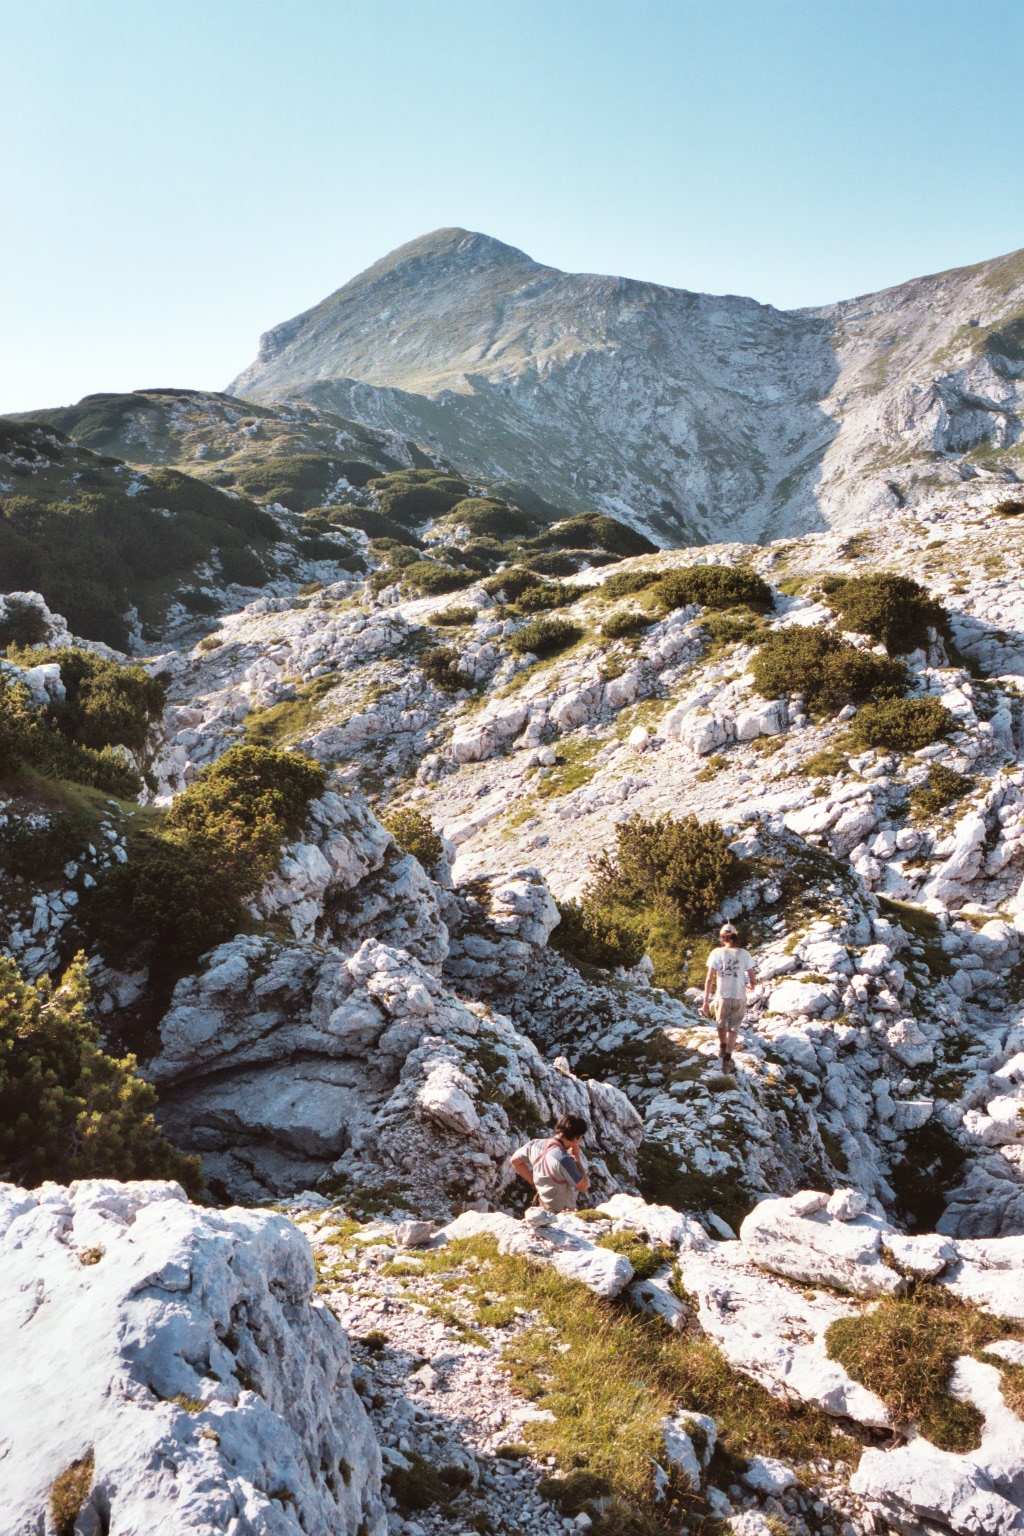
\includegraphics[height=\paperheight]{2007/intro/jarvist frost gr1 film1 -027_24--orig.jpg}}
}
\BgThispage

\section{Expedition Findings}

\margininbox{Logbook}{W566 BFR is our bus of joy, 5.6 metres long

\textbf{Ferries:}

Out on Sat 14th July, 1345 ish, back Sun 12th August, 1100 ish.

Quotes (8-12 weeks in advance): P\&O (9 passengers): 156.25 

With Sea France: 112.00

Sea France (4 weeks in advance): 140 \textbf{BOUGHT}
\protect\mininame{Jarv}}{\logbook}

\begin{marginfigure}
\frame{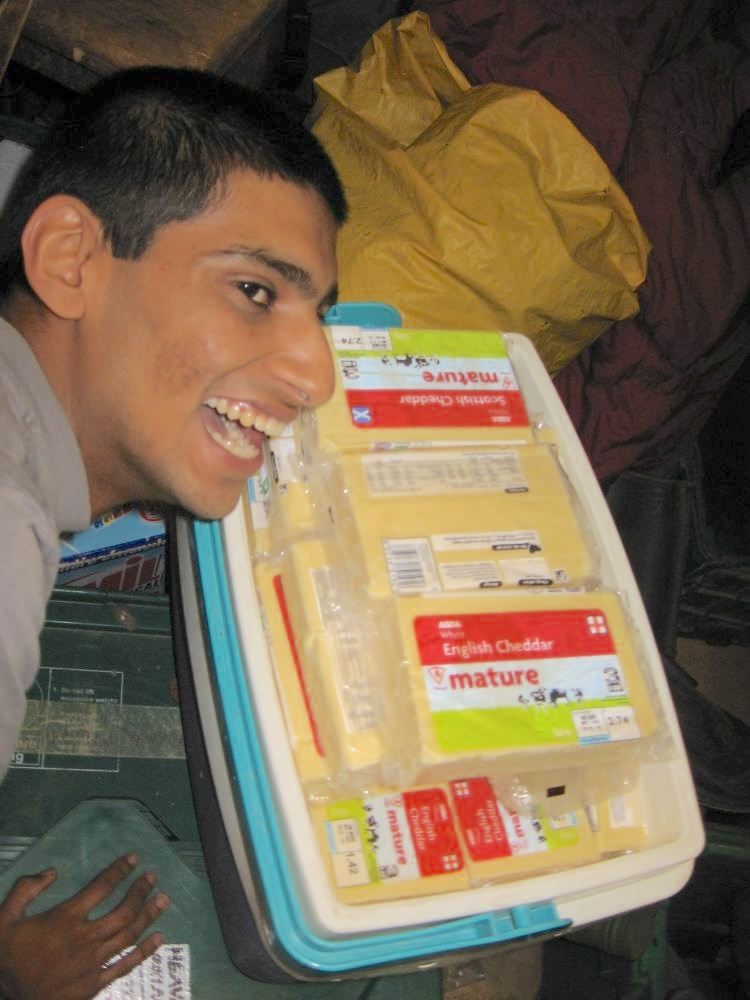
\includegraphics[width=\linewidth]{2007/expedition_findings/jarvist frost - sandeep and cheesus in stores--orig.jpg}}
\caption{Sandeep and cheesus [sic] in stores. \pic{Jarvist Frost}}
\end{marginfigure}

\subsection{\protect\passage{Plop} Goes!}

Andy and Rik pushed \passage{Plop} (the tight squeeze) onto the magnificent
\passage{Plopzilla} pitch. A field of helictites festoon the pitch down onto an
enormous boulder pile. One side of this chamber is unpushed, the other
leads to a boulder choke, as yet unpushed. \passage{Plopzilla} is 105 m
deep, penetrating from \passage{NCB} to below \passage{Exhibition road}. This
makes it the second largest pitch in the system after \passage{Silos}.

\subsection{\protect\passage{M1} \& \protect\passage{M6}}

Repushed + resurveyed. Still a lead (may need chemical persuasion) in a
window off \passage{M1}. Small extensions found in \passage{M6} - very pretty little bit of
stream formed new cave, ended in draughting bedding plane dig.

\subsection{\protect\passage{U-Bend} connected to \protect\passage{Primadona}}

Hard pushing by Sandeep and Alvin through the previously blown \passage{Enigma
squeeze} on the 40 m \passage{U-bend} pitch has led to a connection with the \passage{Drugi Vhod}
entrance to \passage{Primadona}, gaining \passage{Primadona} an additional 57
m of height, making a cave 644 m deep. Beautiful survey accuracy - have
a look on the .3d file!

\subsection{\protect\passage{Razor Cave} survey}

Coordinated by Martin, we've started to survey \passage{Razor Cave}. 250 m
already in the book; it's a very interesting clearly fault-driven cave,
with easy access from the Razor hut.

\subsection{New caves on western edge of plateau}

\begin{pagefigure}
      \checkoddpage \ifoddpage \forcerectofloat \else \forceversofloat \fi
      \centering
              \frame{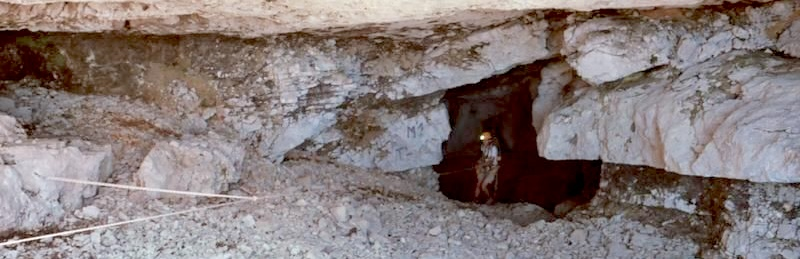
\includegraphics[width=\linewidth]{2007/expedition_findings/jarvist frost gr1 film1 -029_26--orig.jpg}} 
  \caption{The impressive \passage{M1} entrance scree slope. \pic{Jarvist Frost}}
\end{pagefigure}

\passage{Planika} (named after the Edelweiss present on the western plateau) and ``\passage{Monatip}'', found below \passage{B9}/\passage{M21} (on the western edge
of the plateau, approx 100 m north of \passage{Primadona}) and the initial pushing trips conducted. \passage{Planika}: 166 m long, 46 m deep \passage{Monatip}: 196 m long, 28 m deep.

\begin{marginfigure}
\frame{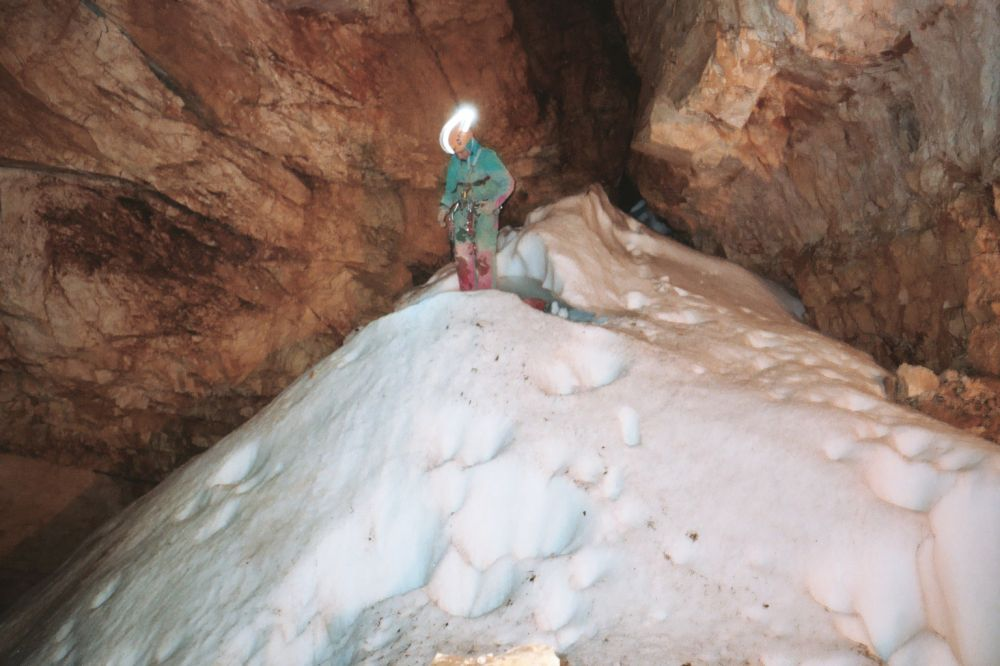
\includegraphics[width=\linewidth]{2007/expedition_findings/jarvist frost gr1 film4 -032_29--orig.jpg}}
\caption{The snow-filled first chamber of \passage{Planika}. \pic{Jarvist Frost}}
\end{marginfigure}

\passage{Planika} is a high entrance (1801 m) which leads directly to a 40 m pitch to a snow plug. Climbing the snow gains another chamber with a large entrance, and a rift leading off. A very tight pitch head at the end of rift leads to a 5 m pitch which reconnects to a 20 m long snow slope. 

Digging at the bottom of this snow slope gained another snow filled chamber, with `phreatic' esque passage etched through the snow by the draught, and extremely drippy snow which I believe is certainly feeding a faithful stream, possibly the one that was found on \passage{Smer0} in \passage{Primadona}, 200 m below. 

To get to \passage{Planika}, one must conduct a 30
m abseil down a cliff, then traverse along the ledge. Extremely pretty - one gets a view across the whole of the Tolminka by day, or the lights of Italy all the way to Venice by night.

\passage{Monatip} is directly below \passage{Planika} (24 m between bottom of snow
plug and early passage), and has a very \passage{NCB}-like character -
possibly a dried river bed. It undulates along, heading into blank
mountain.

\begin{marginfigure}
\frame{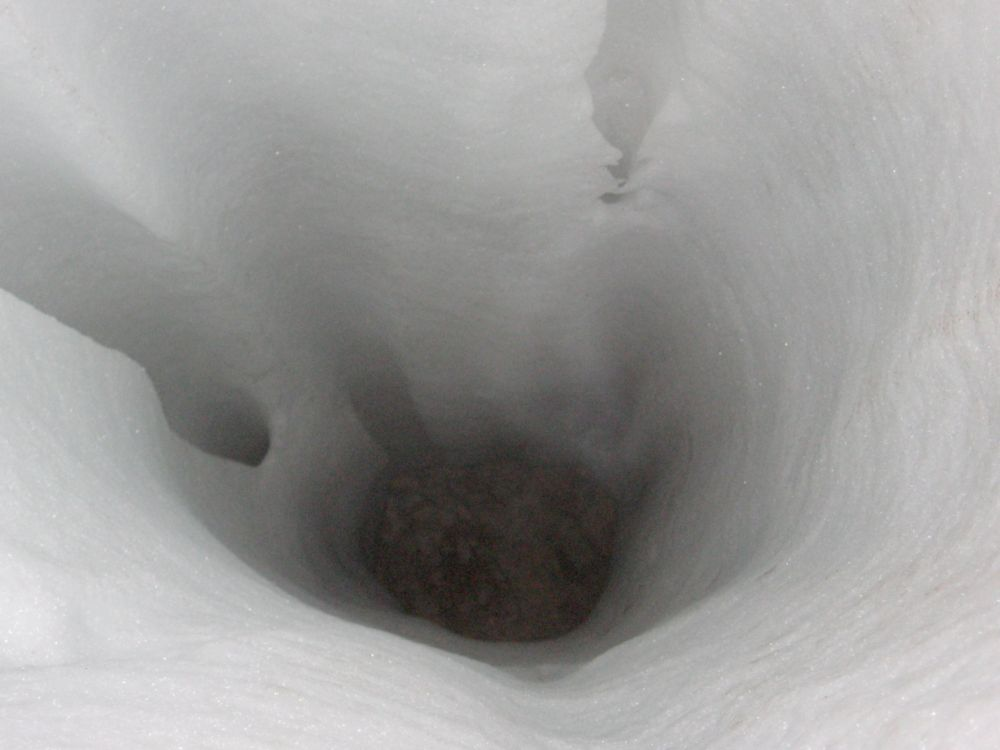
\includegraphics[width=\linewidth]{2007/expedition_findings/jarvist frost - planika first snow chamber - 8m deep hole in snow--orig.jpg}}
\caption{An 8m deep snow hole in \passage{Planika}. \pic{Jarvist Frost}}
\end{marginfigure}

\begin{marginfigure}
\frame{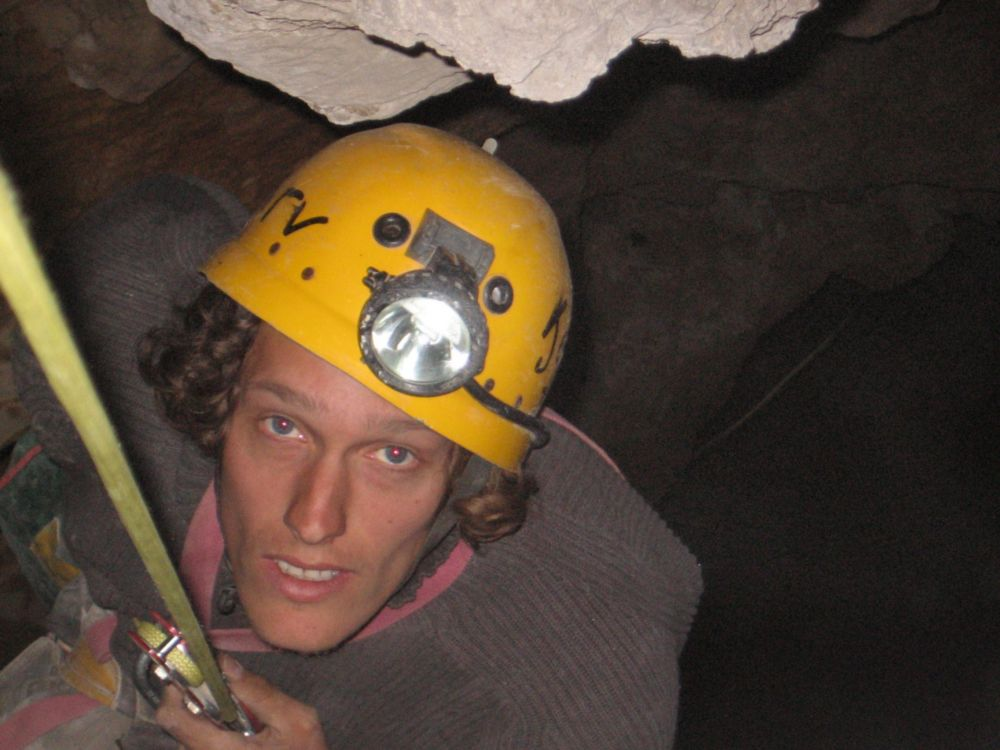
\includegraphics[width=\linewidth]{2007/expedition_findings/jana carga - jarv near rebelay entrance pitch planika--orig.jpg}}
\caption{Jarv descending near the first rebelay in \passage{Planika}. \pic{Jana Čarga}}
\end{marginfigure}


\subsection{\protect\passage{Primadona} \protect\passage{Smer0}
pitch}

Initial rigging of the \passage{Smer0} pitch discovered in October 2006 was
undertaken, bolting down to about -40 m. Pitch is ongoing.
Stream was followed upstream to a tight labyrinth.

\subsection{\protect\passage{Smashed Swede}}

Stefan's climb was bolt-traversed to by Rik and Paul, gaining a window
that would appear to reconnect to \passage{Hardy} Pitch. A second look
wouldn't go amiss.

\section{Minor Caves}

\subsection{\protect\passage{East Pole} (\protect\passage{S1})}

Further work was undertaken in \passage{East Pole} {\passage{S1}). A number of promising new
holes were investigated, including \passage{E1} - a roughly 25 m deep
pitch leading to too-tight windows that require opening up.

\subsection{\protect\passage{Stag Cave}}

A cave was found within 20 m of the tents! A short pitch, rigged on
naturals, lead to a spacious chamber that was unfortunately dead.
However the presence of a large collection of bones (some crushed, but
many in very good condition) that appears to have been from a stag made
up for the disappointment!

\subsection{\protect\passage{Moth Cave}}

\begin{marginfigure}
\frame{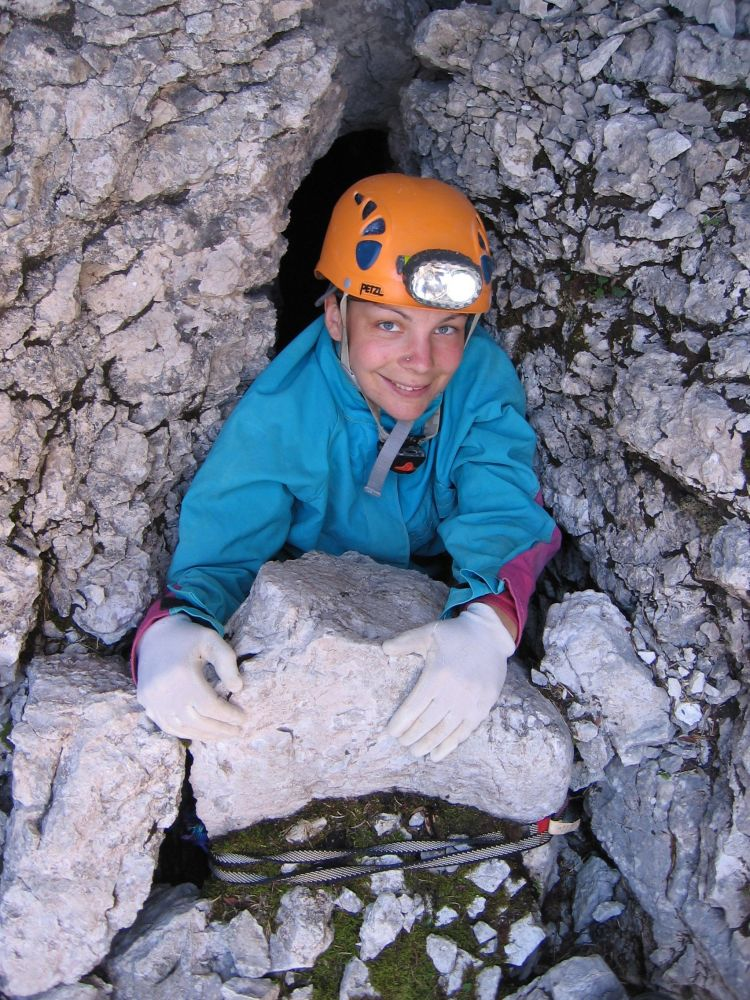
\includegraphics[width=\linewidth]{2007/expedition_findings/jarvist frost - jana entrance to e1--orig.jpg}}
\caption{Jana in the entrance to \passage{E1}. \pic{Jarvist Frost}}
\end{marginfigure}

Heroic effort was expended in the \passage{Moth Cave} dig: two extra chambers were
gained, but unfortunately only lead to yet another too-tight squeeze
requiring rock removal. Declared dead and derigged.

\subsection{\protect\passage{Hawk Cave}}

New (safe) method of gaining the cave was constructed by bolting an
abseil from the cliff-head. Most leads off chamber were found to die, a
bolt traverse was made across the pitch to find an aven where we hoped a
parallel shaft may lie. Still to be revisited - we ran out of time and
rope, and so derigged.

Most of all, this expedition was an enormous training mission: we now
have an extremely strong expedition team together once more, with great
ties to the new JSPDT members.

I think that all the lags can feel extremely proud of the enormous
cannon of information that has been passed on, the new members proud of
the steep learning curve that they all conquered, and everyone proud of
the Caves, little and big, deep and shallow that we've found this year.


\name{Jarvist Frost}

\begin{pagefigure}
      \checkoddpage \ifoddpage \forcerectofloat \else \forceversofloat \fi
      \centering
              \frame{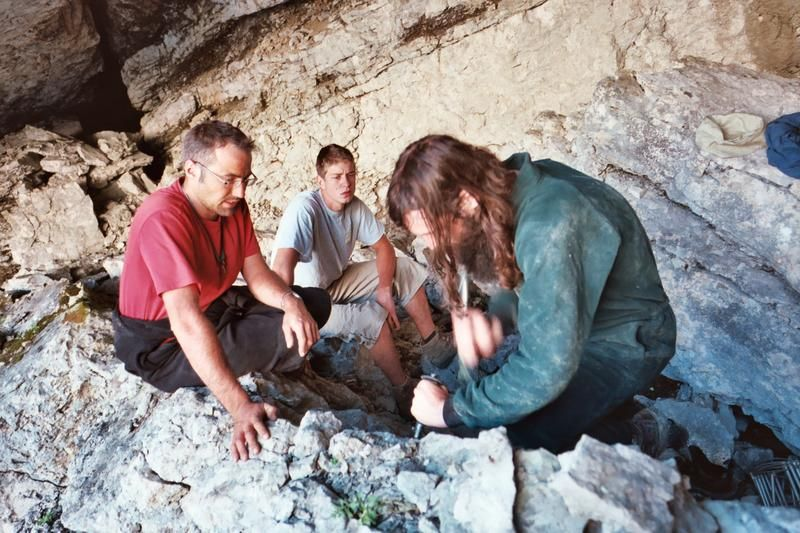
\includegraphics[width=\linewidth]{2007/expedition_findings/jarvist frost gr1 film3 -029_26--orig.jpg}} 
       \label{surface bashing}
  \caption{A surface, quite literally being bashed by James Huggett. \pic{Jarvist Frost}}
\end{pagefigure}


\section{Rik and Andy go to Plop (an abject
Failure)}

\margininbox{Plopzilla}{
     \begin{itemize}
    \item Andrew Jurd
    \item Richard Venn
    \end{itemize}}{\explo}

\textit{Written by Rik in the van on the way back across Europe, later typed up by Jarv.}\\

The mission was simple - venture into \passage{Sistem Migovec}, traverse the gaping
holes on \passage{Level 2} to reach the ratty old rope for \passage{Faulty Towers}
and push into \passage{NCB}. Once there we hoped to bottom the fabled
`\passage{Plop}', a big pitch just off \passage{NCB}, rumoured to be over 50 m,
strongly draughting and utterly jinxed!

Armed only with a vague description from a rather drunken Tetley the
night before, we set off for \passage{M16} during a brief lull in the
raging storm. Once down in the cave we quickly hopped up to \passage{NCB},
reviewing the excellent tourist trip across the big stuff in the system.

When we got to \passage{NCB}, we stumbled as \bignote{Tetley had not mentioned the
lairy traverse} over a $\approx$ 20 m drop on tatty 13-year-old 9
mm. We concluded that \passage{Plop} was the pitch immediately below the rope from
\passage{Torn T-Shirt}. This was the error which cost us the pitch. The bolts continued
down the pitch and I had a sinking feeling as I reached the bottom of
this pointless lead.

After this we inspected the rest of \passage{NCB} going East, crossing the
bad traverse with some care. Andy and I took it in turns to examine the
side passages and one of the ones I inspected was, as in the legend of
'95, a very windy squeeze, which could be depth tested by throwing rocks
with some difficulty. I was sure this was it, but Andy had an earlier
memory which led us to think that it might be \passage{Godzilla}. Stones took
around three or four seconds to drop!

We left with five hours to spare before callout, on the very cautious
side, and left the tackle bags at \passage{NCB}. Tomorrow we're going back,
and this time \passage{Plop} must be conquered!

\name{Richard Venn}



\section{The Eventful Conquest of Plopzilla (née Plop)}

\margininbox{Plopzilla}{
     \begin{itemize}
    \item Andrew Jurd
    \item Richard Venn
    \end{itemize}}{\explo}

After my first trip to \passage{NCB} I was kept awake thinking about that
three to four second drop known simply as `\passage{Plop}'. By eleven the next
morning I'd managed to convince Andy of the merit of a return visit.
Since we'd left the necessary tools and rope for bolting a monster pitch in \passage{NCB}, we quickly shot down the \passage{M16} entrance series and
up \passage{Faulty Towers} into \passage{NCB}.

Fairly terrified of getting stuck in the tight pitch head above that
formidable drop, I took off most of my SRT kit, leaving just cows-tails
and Croll. The squeeze was fairly easy and Andy passed through the bags as I put in a bolt to make a Y-hang.

Since \passage{Plop} had already been attempted several times there were quite a few existing bolts. I made use of these on the way, stopping only to take down a couple of boost bars: \bignote{a bit of Cadbury Courage}. I felt oddly calm swinging about in the huge chamber. We had thrown more rocks from the top but the bottom was too far away to see. Even from the first rebelay I was having trouble speaking to Andy. Our words boomed around the huge pitch. Two rebelays down, \bignote{I was standing on a gravel floor, shivering with the adrenaline}. I'd been forced to put in a knot pass in the rope and reverse prussic past it. Two more bolts got us to the bottom of the pitch, by which point our nerves were totally shredded.
Though the hang of the rope was very clean, a rope disappearing into
empty blackness above can be really terrifying!

Though we were almost expecting to break into `Level 3', an as-yet
undiscovered horizontal passage at least three kilometres long, the
pitch was completed choked with boulders at its lowest point. We scoured
the nooks and crannies before pronouncing the bottom of \passage{Plop} officially
dead.

However, twenty metres back up the gravel slope, another boulder choke
went down, an obvious lead for a return visit but by this stage we were
too tired to push and survey a new cave passage. We left a going lead in
boulders, along with an easy swing into a window halfway down the pitch.

Exit from the cave was difficult due to being tired and thirsty but \bignote{we were in a jubilant mood after a seventy-six metre survey leg!} \passage{Plop} was the biggest pitch either of us had ever seen. As the first to bottom
this monster, we renamed it `\passage{Plopzilla}'. Analysing the survey data back at the bivi, it measured in at an
impressive 105 m of depth.

\name{Richard Venn}

\begin{pagefigure}
      \checkoddpage \ifoddpage \forcerectofloat \else \forceversofloat \fi
      \centering
              \frame{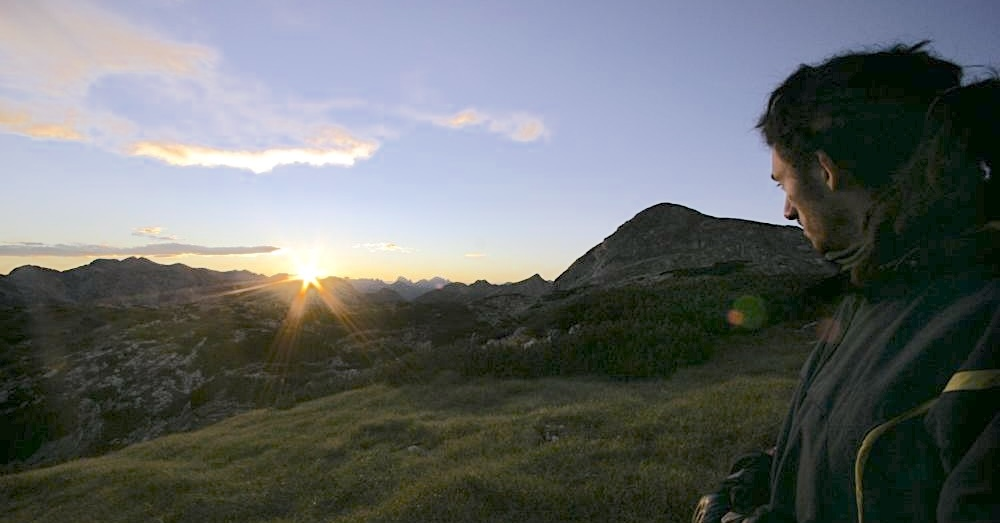
\includegraphics[width=\linewidth]{2007/plop/martin mcgowan -rik watching sunset--orig.jpg}} 
  \caption{Rik watching the setting sun from sunset spot. \pic{Martin McGowan}}
\end{pagefigure}

\section{Riggin' Captain Kangaroo}

\margininbox{Captain Kangaroo}{
     \begin{itemize}
    \item Tharatorn Supasiti
    \item Richard Venn
    \end{itemize}}{\explo}

First trip was with Thara. Tet had already rigged down \passage{Pico} (re-bolting
it in the process), so we set off for that familiar window with a
bolting hammer, a hundred metres of rope and a couple of cinnamon malt
loaves. Had the same trouble finding Tet's single bolt as I'd had in
2005. However, instead of bottling it, I placed two new spitz, this time
within sensible reach for easy rigging. A hundred metres of rope got us
to \passage{Traverse Chamber}, cursing and kicking the heavy bag all the way
through \passage{Scrotty}.

\margininbox{Captain Kangaroo}{
     \begin{itemize}
    \item Sandeep Mavadia
    \item Richard Venn
    \end{itemize}}{\explo}

    \margininbox{Captain Kangaroo}{
     \begin{itemize}
    \item James Huggett
    \item Richard Venn
    \end{itemize}}{\explo}

Sandeep was the next victim, this time we set off with a hundred and
fifty metres of rope. We rigged down to \passage{Olympic Rift}, stopping on the
way to chisel open an awkward squeeze. We left thirty metres of rope in
a tacklesack at the start of \passage{Olympic Rift} and did some re-bolting on the
last two pitches. Also left three hangers and maillons, ten spits \&
cones, two karabiners, a chisel and two slings. At this stage the
squeeze and huge black space the other side at the end of \passage{Olympic rift}
seemed like the best lead in \passage{Captain Kangaroo}.

A bounce to \passage{Pico} with James gave me the chance to do some more work on
the entrance to \passage{Captain Kangaroo}. I put in a tensioned traverse which
removed the `traditional' rub-point at the start of the take off.

\name{Richard Venn}


\section{Pushin' Captain Kangaroo}

\margininbox{Captain Kangaroo}{
     \begin{itemize}
    \item Ben Banfield
    \item Richard Venn
    \end{itemize}}{\explo}

I had hoped that keen cavers would rush into \passage{Captain Kangaroo} to push
the more shallow lead off \passage{Traverse Chamber}, leaving me to go and smash
open \passage{Olympic Rift} to fame and great glory in whatever gaping chasm lay
beyond the terminal squeeze. Unfortunately, Vom-Brown\sidenote {Tom Brown} and the Deep\sidenote {Sandeep Mavadia}
turned back near \passage{Bonus Chamber}, with `visions of hell' muttered back at
the bivvi from the first sign of mild scrotty-ness.

I collared young Ben in the bivvi over a generous swig or two of
rum-spiked tea and we hatched a plan to crawl along a tight rift that
I'd looked down with Jarv in 2005, but been unable to survey due to lack
of tape. With survey pencils and instruments in tow, we slipped through
the cave to the pushing front and stripped off SRT kits to pass more
easily through the rift. This was somewhat tighter than I'd remembered
and shredded my PVC oversuit.

\bignote{We pushed as far as we dared survey}, breaking out right at the end into a
large double chamber with several leads coming off. The most obvious of
these was a climb down into what looked like walking passage.

Returning a few days later with Izzy\sidenote {Izi Možir} from Tolmin, with a bag of rope and
bolting kit, we pushed the passage another fifty metres or so. Some
gardening of large rocks was required to pass a short section of rift
but we were mostly in big passage, clambering down rather sharply over a
series of climbs.

\begin{marginfigure}
\frame{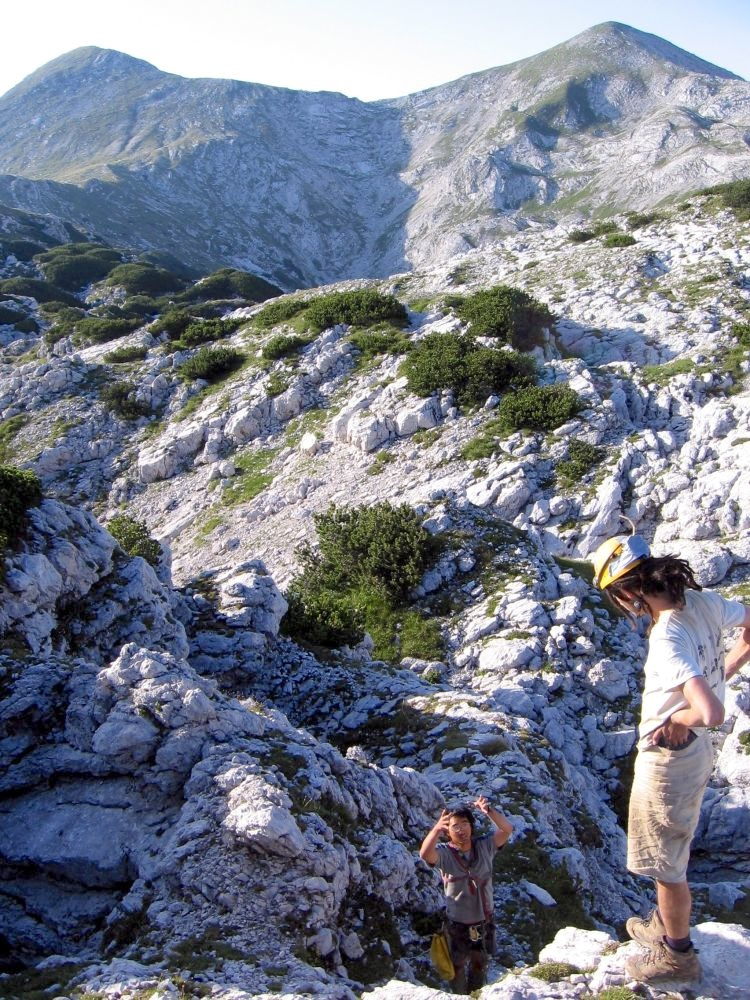
\includegraphics[width = \textwidth]{2007/kangaroo/jarvist frost - m1 - rik and thara after bolting--orig.jpg}}
\caption{Rik and Thara after their bolting trip, standing beside \passage{M1}. \pic{Jarvist Frost}}
\end{marginfigure}

\margininbox{Kill'em All}{
     \begin{itemize}
    \item Iztok Možir
    \item Richard Venn
    \end{itemize}}{\explo}

Eventually we reached a point where a big passage closed up to about one
or two metres of very tight rift with a big ($\approx$ two second) drop on
the other side. This was passable but looked more than a little
unpleasant without some serious work with a chisel.

We looked around the chamber a little more before discovering a tight
sharp crawl which dog-legged before coming out in beautiful white rock
at the top of a twenty metre pitch. Izzy belayed my full weight from
within the crawl while I put in the two bolts. This allowed us to
descend to the bottom of the pitch with a few metres of rope to spare.
This is possibly not the same pitch we were throwing rocks down through
the tight rift but obviously very close!

As we dropped the pitch there were windows on both sides looking like
they came from either other pitches or more rift-like development as
well as two leads at the bottom. These were a small \passage{Captain Kangaroo}-esque rift and ten or twenty metres more of the pitch. We left
$\approx$ 10 m of rope, but took the tacklesack out.

This was a very exciting new section of passage. We named the contents
of our push ``\passage{Kill'em All}'' after the first Metallica album. Upon
inspection of our survey data, it became clear that we were exceedingly
close to passage below \passage{Silos}/\passage{Godzilla} in \passage{M2} (less than thirty
metres at closest approach).

Unfortunately, a month on \passage{Migovec} was starting to catch up with me and
though I wanted another trip in \passage{Gardeners' World} to push \passage{Olympic rift}, I
was completely exhausted with very sore knees. The leads we left in
\passage{Captain Kangaroo} this year will be far too tantalising to sideline in favour of
surface work in 2008. The prospect of a connection with the system seems
very likely and next year we're already planning a return to \passage{M2}
to resurvey (our current data comes from a 1970s survey carried out with
a home-built clinometer!) and to exhaust the deep leads.

\name{Richard Venn}

\begin{figure}
\checkoddpage \ifoddpage \forcerectofloat \else \forceversofloat \fi
   \centering
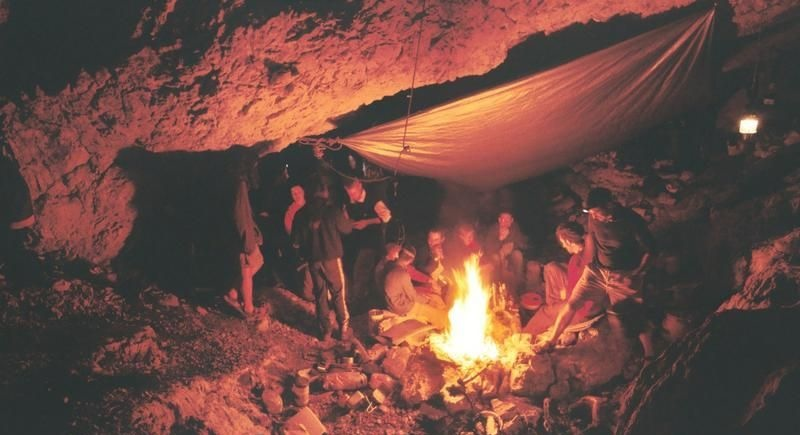
\includegraphics[width = \textwidth]{2007/kangaroo/jarvist frost gr1 film2 -031_28.jpg}
\caption{A typical evening in the bivi around the fire. \pic{Jarvist Frost}}
\end{figure}

\begin{pagesurvey}
\centering
\frame{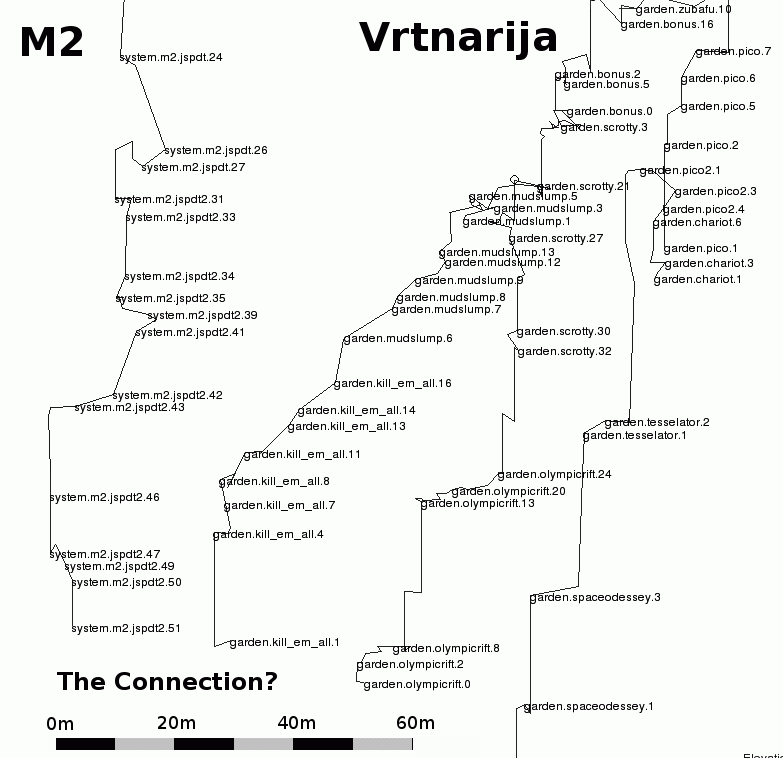
\includegraphics[width=\textwidth]{2007/kangaroo/survex - 2007 data - m2 vrtnarija closest approach--orig.png}}
\caption[M2 Vrtnarija Closest Approach]{Survey data of the closest approach between \passage{M2} and \passage{Gardeners' World}.}
\label{plan 2013}
\end{pagesurvey}

\section{Bolting ``Kill'em All''}

\margininbox{Kill'em All}{
     \begin{itemize}
    \item Izi Možir
    \item Richard Venn
    \end{itemize}}{\explo}

During the ever long breakfast in the Bivy, Rick was asking who wants to
go with him to \passage{Captain Kangaroo}. Nobody volunteered immediately. Tetley
said he can go, but only to \passage{Bonus chamber} and then pointed to me and
said, ``Izi, you should go!'' I agreed and soon we were packing all the
necessary equipment.

This was my first time in \passage{Vrtnarija} and at the beginning was nothing to
serious, lovely pitches, couple of squeezes and soon we were on top of
\passage{Pico}. Rick warned me to use the red rope, which is going right into the
\passage{Captain Kangaroo}. Before we enter the Captain Rick said, ``So, this is
it! Now fun begins!'' We all smoked one and off we go. Tetley turned
back at \passage{Bonus chamber}. Rick knew the way on so he was the leader. We
soon arrived to \passage{Mudslump} with few very tight and tricky squeezes.

\begin{marginfigure}
\checkoddpage \ifoddpage \forcerectofloat \else \forceversofloat \fi
\centering
 \frame{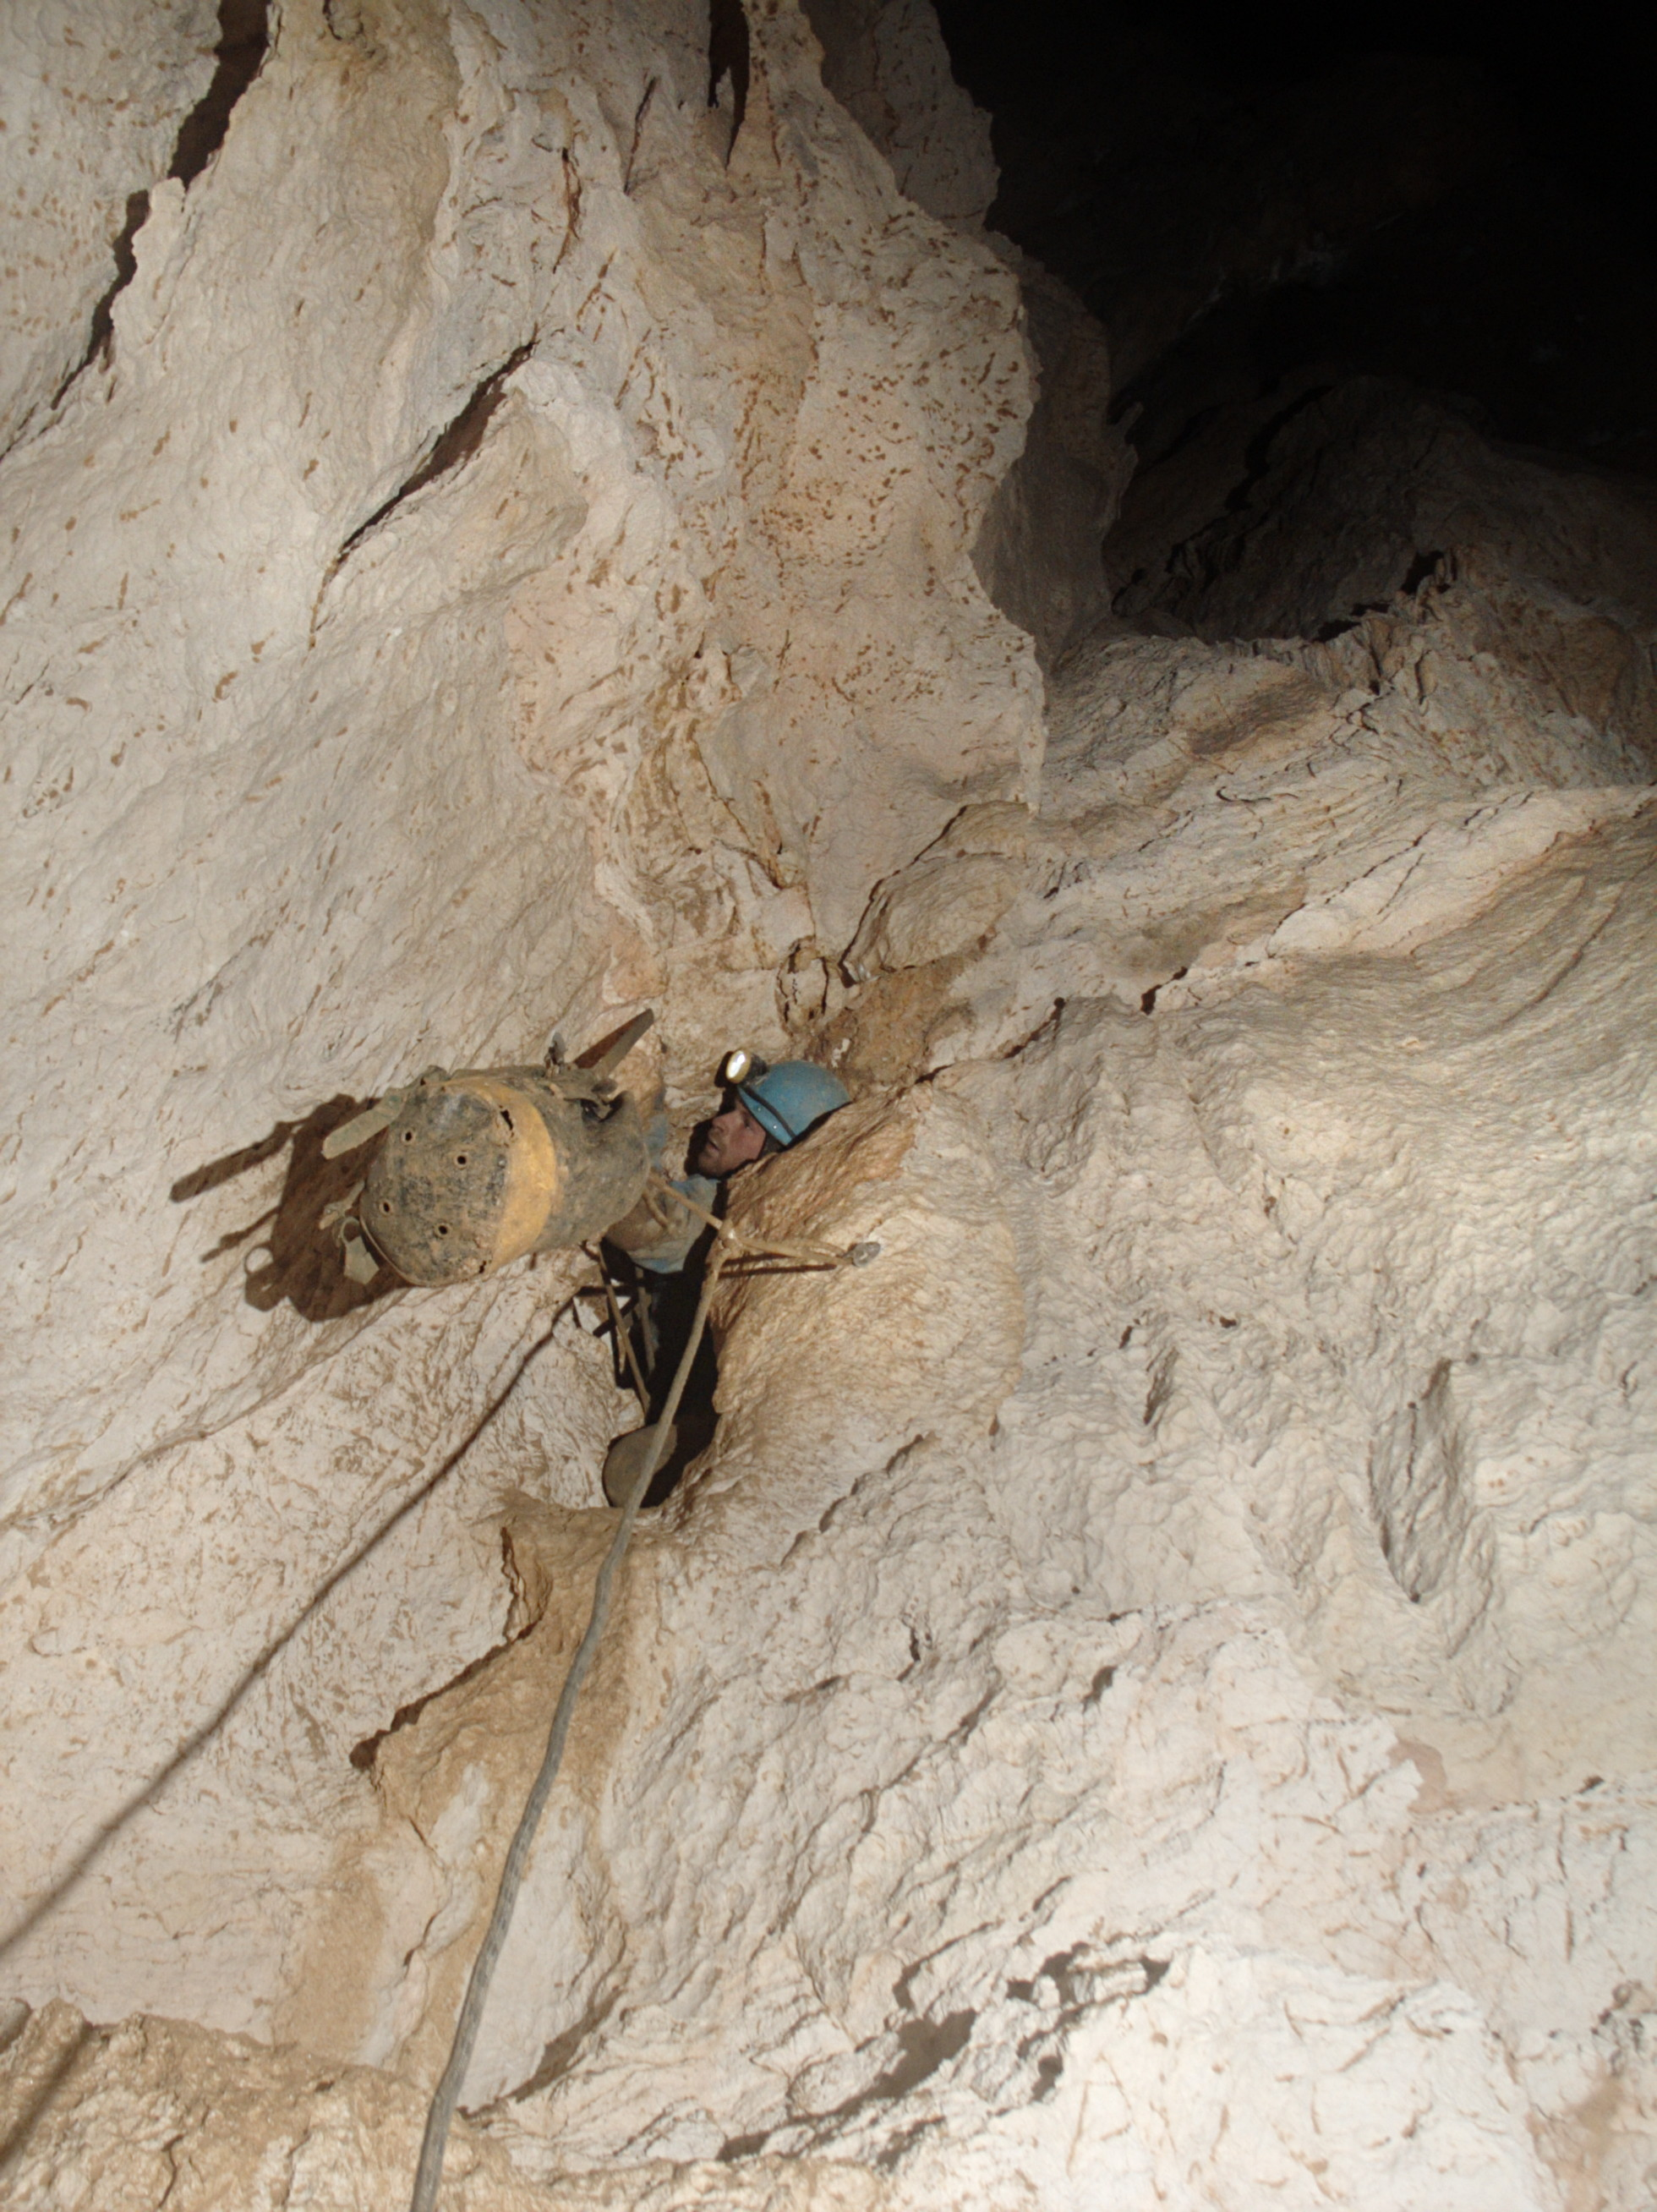
\includegraphics[width=\linewidth]{2007/kill_em_all/2009-08-06-15.01.44 - Jarvist Frost - Canon Powershot G5 - killem all - mike at pitch head struggling with bag--orig.jpg}} 
 \caption{Mike Foley struggles with a tackle bag at the pitch head of \protect\passage{Kill'em All} in 2009 while Jarvist Frost waits on the rope below. \pic{Jarvist Frost}}
 \label{Kill em All Mike}
\end{marginfigure}

Once through, we free climbed couple of small pitches and arrived to a
small chamber. The way on was through a squeeze which led to a top of
the pitch. It was very little space here, not even enough to do the
bolting properly. After couple of minutes of thinking and couple of
cigarettes we had a plan. One of us would go on the rope, while the
other one will attach the rope to his croll, get stuck in the squeeze
and hold the other one until bolting finished. Rick was brave enough to
trust me, so he did the bolting. During the bolting I smoked a lot and
we chatted about the music. We both knew the first Metallica album and
so we decide to name this pitch \passage{Kill'em All}. The way down was no
problem and while descending we spotted lots of windows. On the bottom
we cut the rope, leave the rest there and started surveying on way out.
Rick went up first and it took him a while to get the rope free. 

Finally, I went up and soon realised what took Rick so long. When we were bolting
we were not paying attention on how low the bolts are. Now \bignote{the only way
to go off the rope was to undo your croll and step into the Y hang and
somehow throw yourself into the pitch head squeeze}. Overall, a very
enjoyable caving journey with Rick. Once in the bivy, we entered the
data into Survex and we realised we were very close to the bottom of
\passage{Silos} (\passage{M2}).

\name{Izi Možir}




\section{\texorpdfstring{First time in
\emph{M16}}{First time in M16}}

\margininbox{M16}{
     \begin{itemize}
    \item Erik Bončina
    \item James "Tetley" Hooper
    \item Izi Možir
    \end{itemize}}{\explo}

It was my first year on Mig and I was very excited to go caving and join
the ICCC on top. Till now, we were only caving in \passage{Primadona} while
staying at \passage{Kal}. One day Erik and I decided to go and rather than sleep
at \passage{Kal}, sleep on top with the English. We stayed up for a couple of
days. Our first caving trip was in \passage{M16}. Tetley took us to the
bottom of \passage{Sajeta}. From \passage{XXX} onwards Tetley was unsure of the rope and
said that his brains are telling him not to go further, but his heart
wants to go. Tetley descended \passage{Sajeta} first, followed by myself and then
Erik. When I arrived at the bottom, Tetley was acting really seriously
and said to me ``What are you doing here?'' I was bit confused why is he
asking me that and thought we should not follow him down. He then asked
me the same question couple of times which made me even more confused.
On the end I finally said to him, that I am here to cave. He then
replied ``If you are on holidays, \bignote{why are you here and not chasing girls
on Croatia beach?}'' We start laughing. Same happened to Erik.

On the way out Tetley was rushing us to get out (we were leading the way
to memorise the cave), as he did not want to miss the call out. At that
time we did not know what a call out was and so we speeded up. On the
end I was really tired, but it was worth it.

\name{Izi Možir}

\begin{pagefigure}
\checkoddpage \ifoddpage \forcerectofloat \else \forceversofloat \fi
   \centering
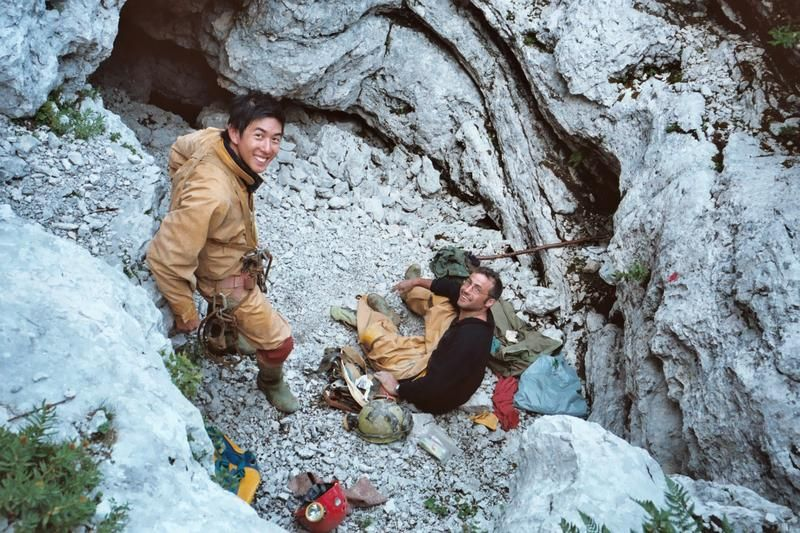
\includegraphics[width = 0.9\textwidth]{2007/m16/jarvist frost gr1 film1 -004_1--orig.jpg}
\caption{Alvin and Tetley in the entrance shakehole to \protect\passage{M16}. \pic{Jarvist Frost}}
\end{pagefigure}

\section{Alex Pitcher Report}

\fullwidthbox[\award]{The Alex Pitcher Memorial Award}{
     The Alex Pitcher Memorial Award is an individual grant from the Ghar Parau Foundation (GPF) awarded to young cavers. Alex Pitcher was a young caver who lost his life on an expedition to the \passage{Gouffre Berger} in the late 1980s. His memorial fund was established to support young cavers (under the age of 25) going on their first expedition outside the UK or Ireland. It is usually put towards training and/or personal equipment costs for such individuals. One or two awards are made each year per GPF Expedition Grant Application, in the order of £100 each.}

\margininbox{Alex Pitcher, 2007}{Ben Banfield received the Alex Pitcher memorial fund award to support his first caving expedition, and wrote a report of his time on expedition for the GPF. His report is replicated here.}{\award}

This summer I was a member of Imperial College Caving Club's expedition to \passage[mountain]{Tolminski Migovec} in the Julian Alps in Slovenia. The club has been running the expedition for over a decade now and I was looking forward to improving my caving skills and techniques as well as contributing to the knowledge about the caves under the \passage{Migovec plateau}. The Alex Pitcher Memorial Fund kindly awarded me some money which helped me purchase my own helmet and helmet mounted light. Having my own helmet mounted light was essential to my participation in the expedition, as the club only owns FX3's with batteries on a belt that are unsuitable for \passage{Migovec} due to the batteries needing a mains. Below is a report of most of my caving activities during the expedition.


\subsection{Wednesday 18th (July)}

After being suggested as \bignote{a lead with a lot of potential and a good place
for budding cave explorers}, Tom Brown and myself set off for \passage{Moth Cave},
in shorts, t-shirts, knee-pads and helmets for a look. Spent a few hours
shifting boulders and scree 15 m into the cave at the pushing front,
before leaving. Has a gusting draught at the pushing front. Will return
again with tools and proper clothing for a better look.

\subsection{Thursday 19th}

\margininbox{Moth Cave}{
     \begin{itemize}
    \item Ben Banfield
    \item Tom Brown
    \item Alvin Chow
    \end{itemize}}{\explo}

Alvin joined Tom and myself today to continue pushing the lead in \passage{Moth
Cave}. After a few rotations of digging we had a badger sized hole and
decided to stop for lunch. Afterwards more excavating around the \passage{Badger
Hole} and scree slope occurred. Several animal bones were recovered from
the scree. An ominous slab of rock sat at the top of the scree making
progress tenuous. Further digging around the badger hole led to another
badger sized tunnel off to the left of the original. After moving 45-50
bags of scree we called it a day. Out 8pm with plans to ask about
explosives for further pushing.

\begin{figure*}[t!]
\checkoddpage \ifoddpage \forcerectofloat \else \forceversofloat \fi
\frame{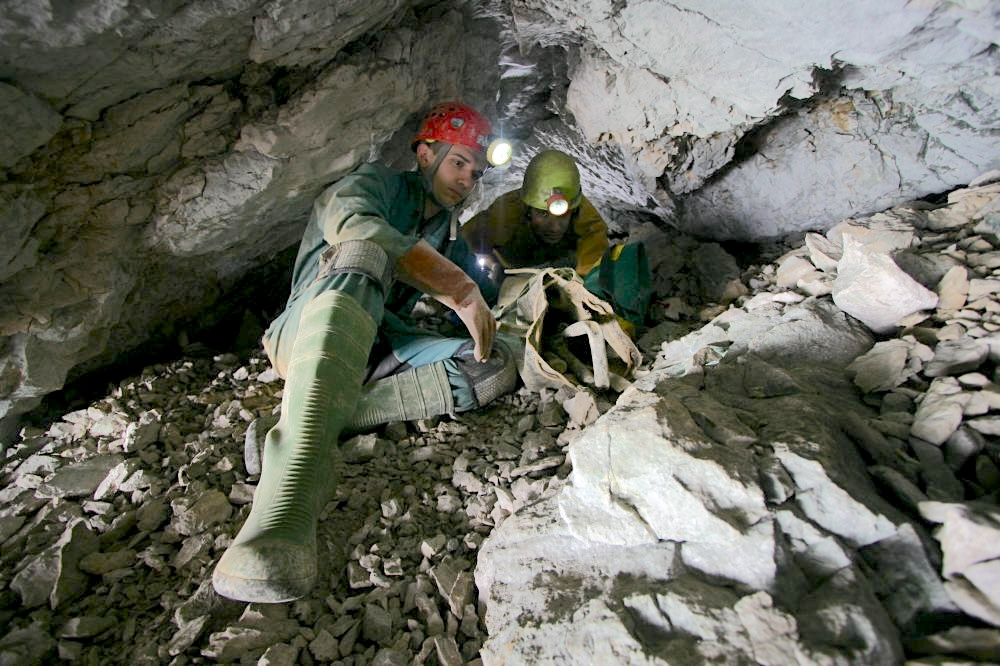
\includegraphics[width=\linewidth]{2007/ap_memorial_award/martin mcgowan -sandeep and ben in moth cave entrance--orig.jpg}}
\caption{Ben and Sandeep in the entrance to \protect\passage{Moth Cave}. \pic{Martin McGowan}}
\end{figure*}

\subsection{Friday 20th}

A short look at \passage{Moth Cave} with t-shirts and shorts again with Martin to ask
about explosives and other digging options. \bignote{Moved the ominous boulder at
the top of the scree to ease our minds} about becoming crushed. The
bottom of the scree slope was dug to more resemble a trench for easier
access to the pushing front.

\subsection{Sunday 22nd}

With the potential for leads and the fact that \passage{Moth Cave} lies on top of the
\passage{System Migovec} / \passage{Primadona} connection area, linking it into the
main survey was a priority. Martin taught several of us the essentials
of surveying while we surface surveyed to \passage{Moth Cave} entrance. Alvin and Thara
continued digging while Martin, Tom and myself surveyed to the pushing
front. 6 survey stations later we joined up with the digging team. Using
various combinations of left and right-handers we made a lot of progress
expanding the left hand badger hole and the trench. \bignote{Breakthrough looking
likely tomorrow}.

\subsection{Tuesday 24th}

After a day's break I rejoined the \passage{Moth Cave} pushing team. Sandeep had joined
us and almost straight away he managed to squeeze through the tunnel
(now named \passage{Badger Highway}) and into a small chamber. Alvin and myself
then made it through and throughout the afternoon work commenced on
enlarging \passage{Badger Highway} from the other end, to make it accessible to
larger cavers. The chamber contained going leads. One, a long
crawl/squeeze that needed enlarging had most potential.

\subsection{3rd week of expedition}

After proving to be such a promising lead before the expedition and
during the first two weeks, \passage{Moth Cave} needed the final push to see
whether it goes or dies. The day prior the petrol drill joined us to try
and enlarge \passage{Badger Highway} to allow more people to reach the pushing
front. Unfortunately the drill was more of a hindrance than a help,
fuming the cave and not expanding the passage.

\begin{marginfigure}
\frame{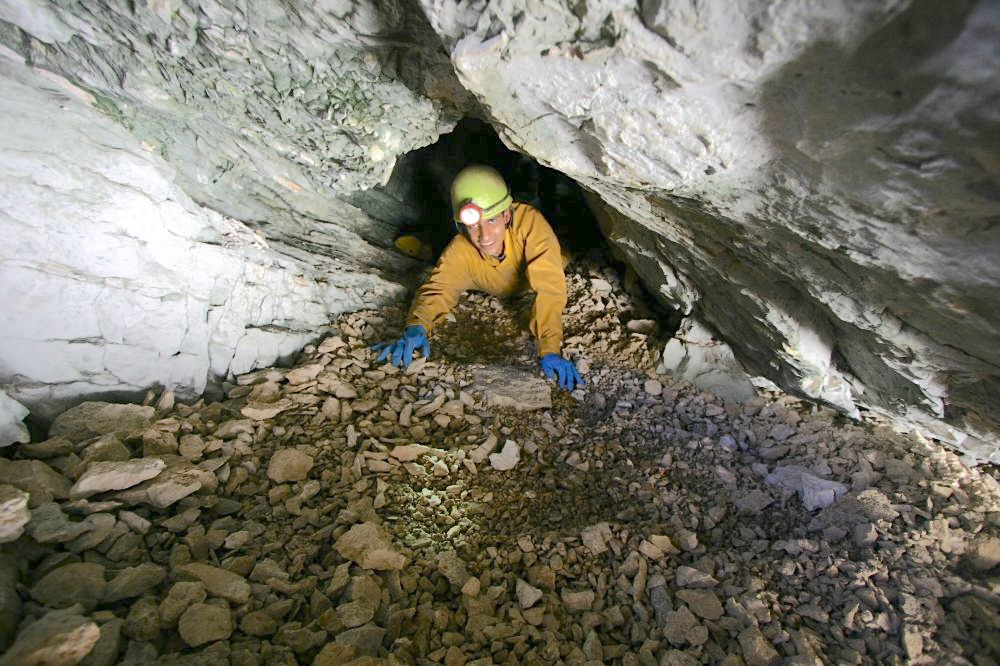
\includegraphics[width=\linewidth]{2007/ap_memorial_award/martin mcgowan -sandeep in moth cave--orig.jpg}}
\caption{Sandeep in the entrance to \protect\passage{Moth Cave}. \pic{Martin McGowan}}
\end{marginfigure}

With no draught coming from the pushing front or even through \passage{Badger
Highway} any more, hopes for a breakthrough didn't look promising.
Everyone else had plans for the next day, so armed with a survey kit and
some bright red nail varnish, I took on the mission of completing the
survey and exploring all available leads.

The squeeze through the tunnel looked more daunting than ever, but with
the knowledge a call-out team would be along within a few hours, I
pushed through. Minor digging allowed me further access along the main
lead. Another small chamber with no going leads was found. The nail
varnish came in useful to mark a permanent survey station. Taking all
digging tools and the survey notes out, I was back to camp well before
my call-out and in time for a nice rest in the sun.



\begin{pagefigure}
      \checkoddpage \ifoddpage \forcerectofloat \else \forceversofloat \fi
    \centering
    \begin{subfigure}{0.49\textwidth}
        \frame{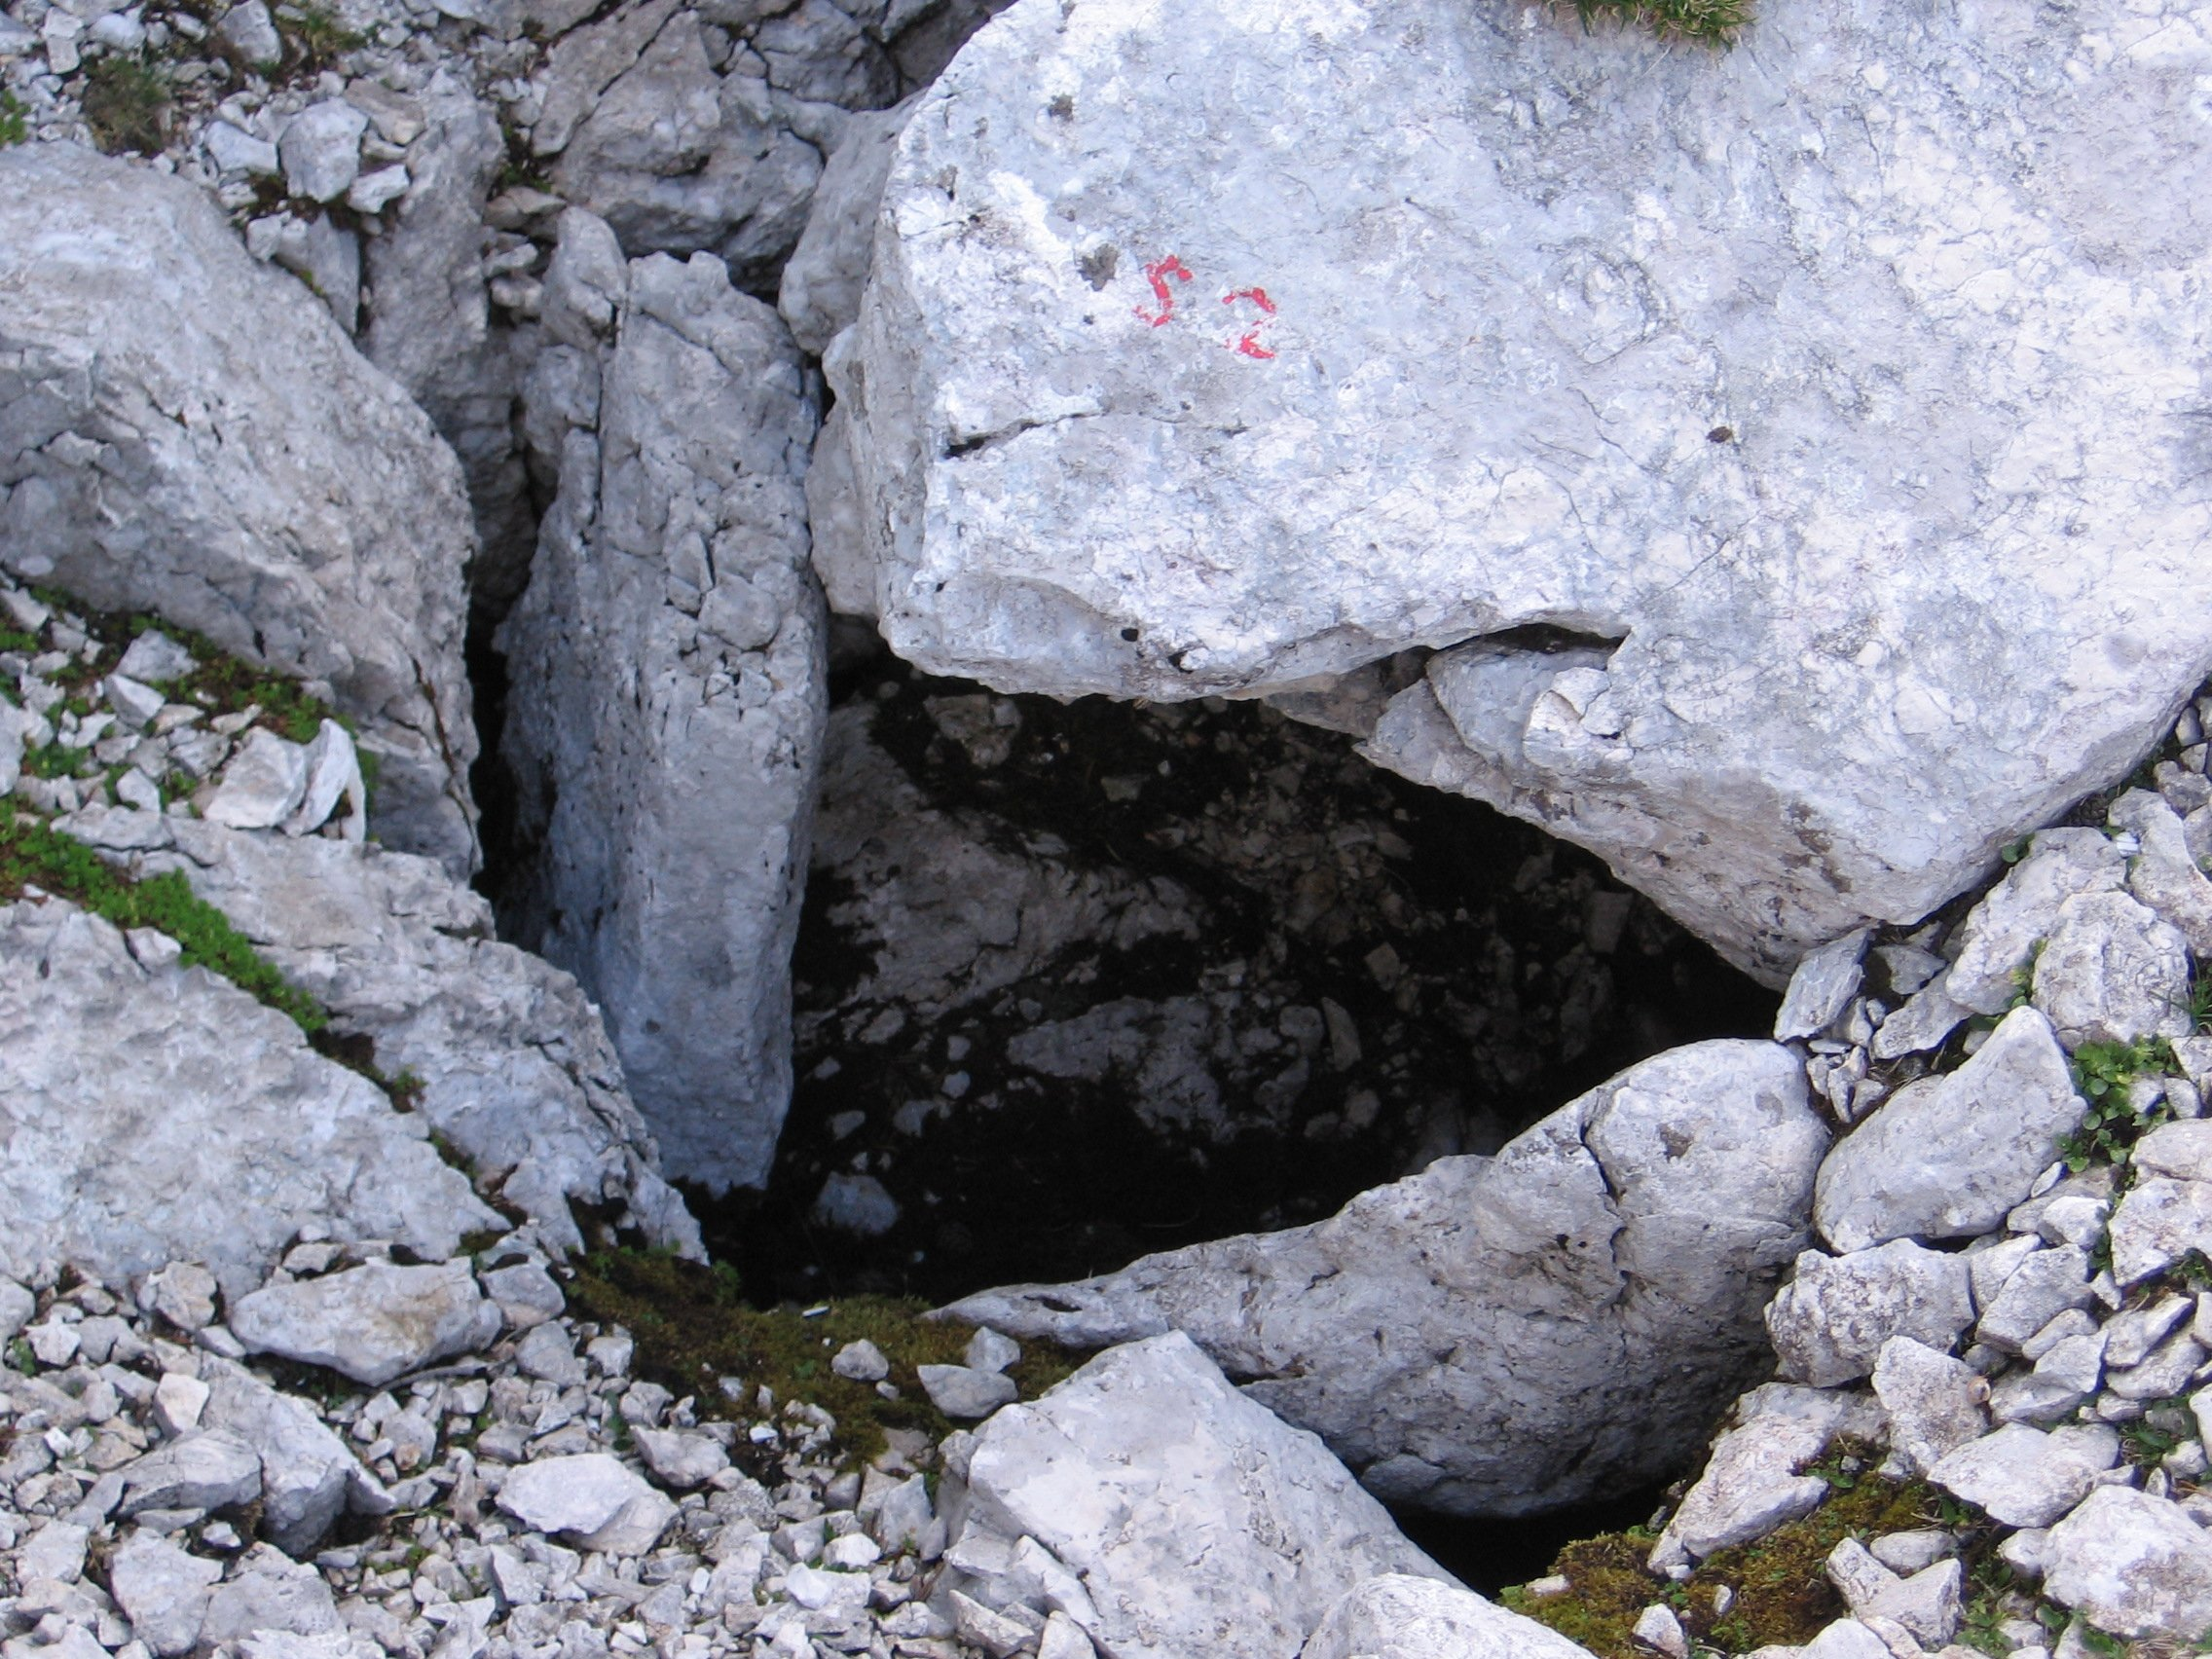
\includegraphics[width=\linewidth]{2007/S/jarvist frost - s2 entrance--orig.jpg}}
        \caption{\protect\passage{S2}}
    \end{subfigure}
\hfill
    \begin{subfigure}{0.49\textwidth}
    \centering
        \frame{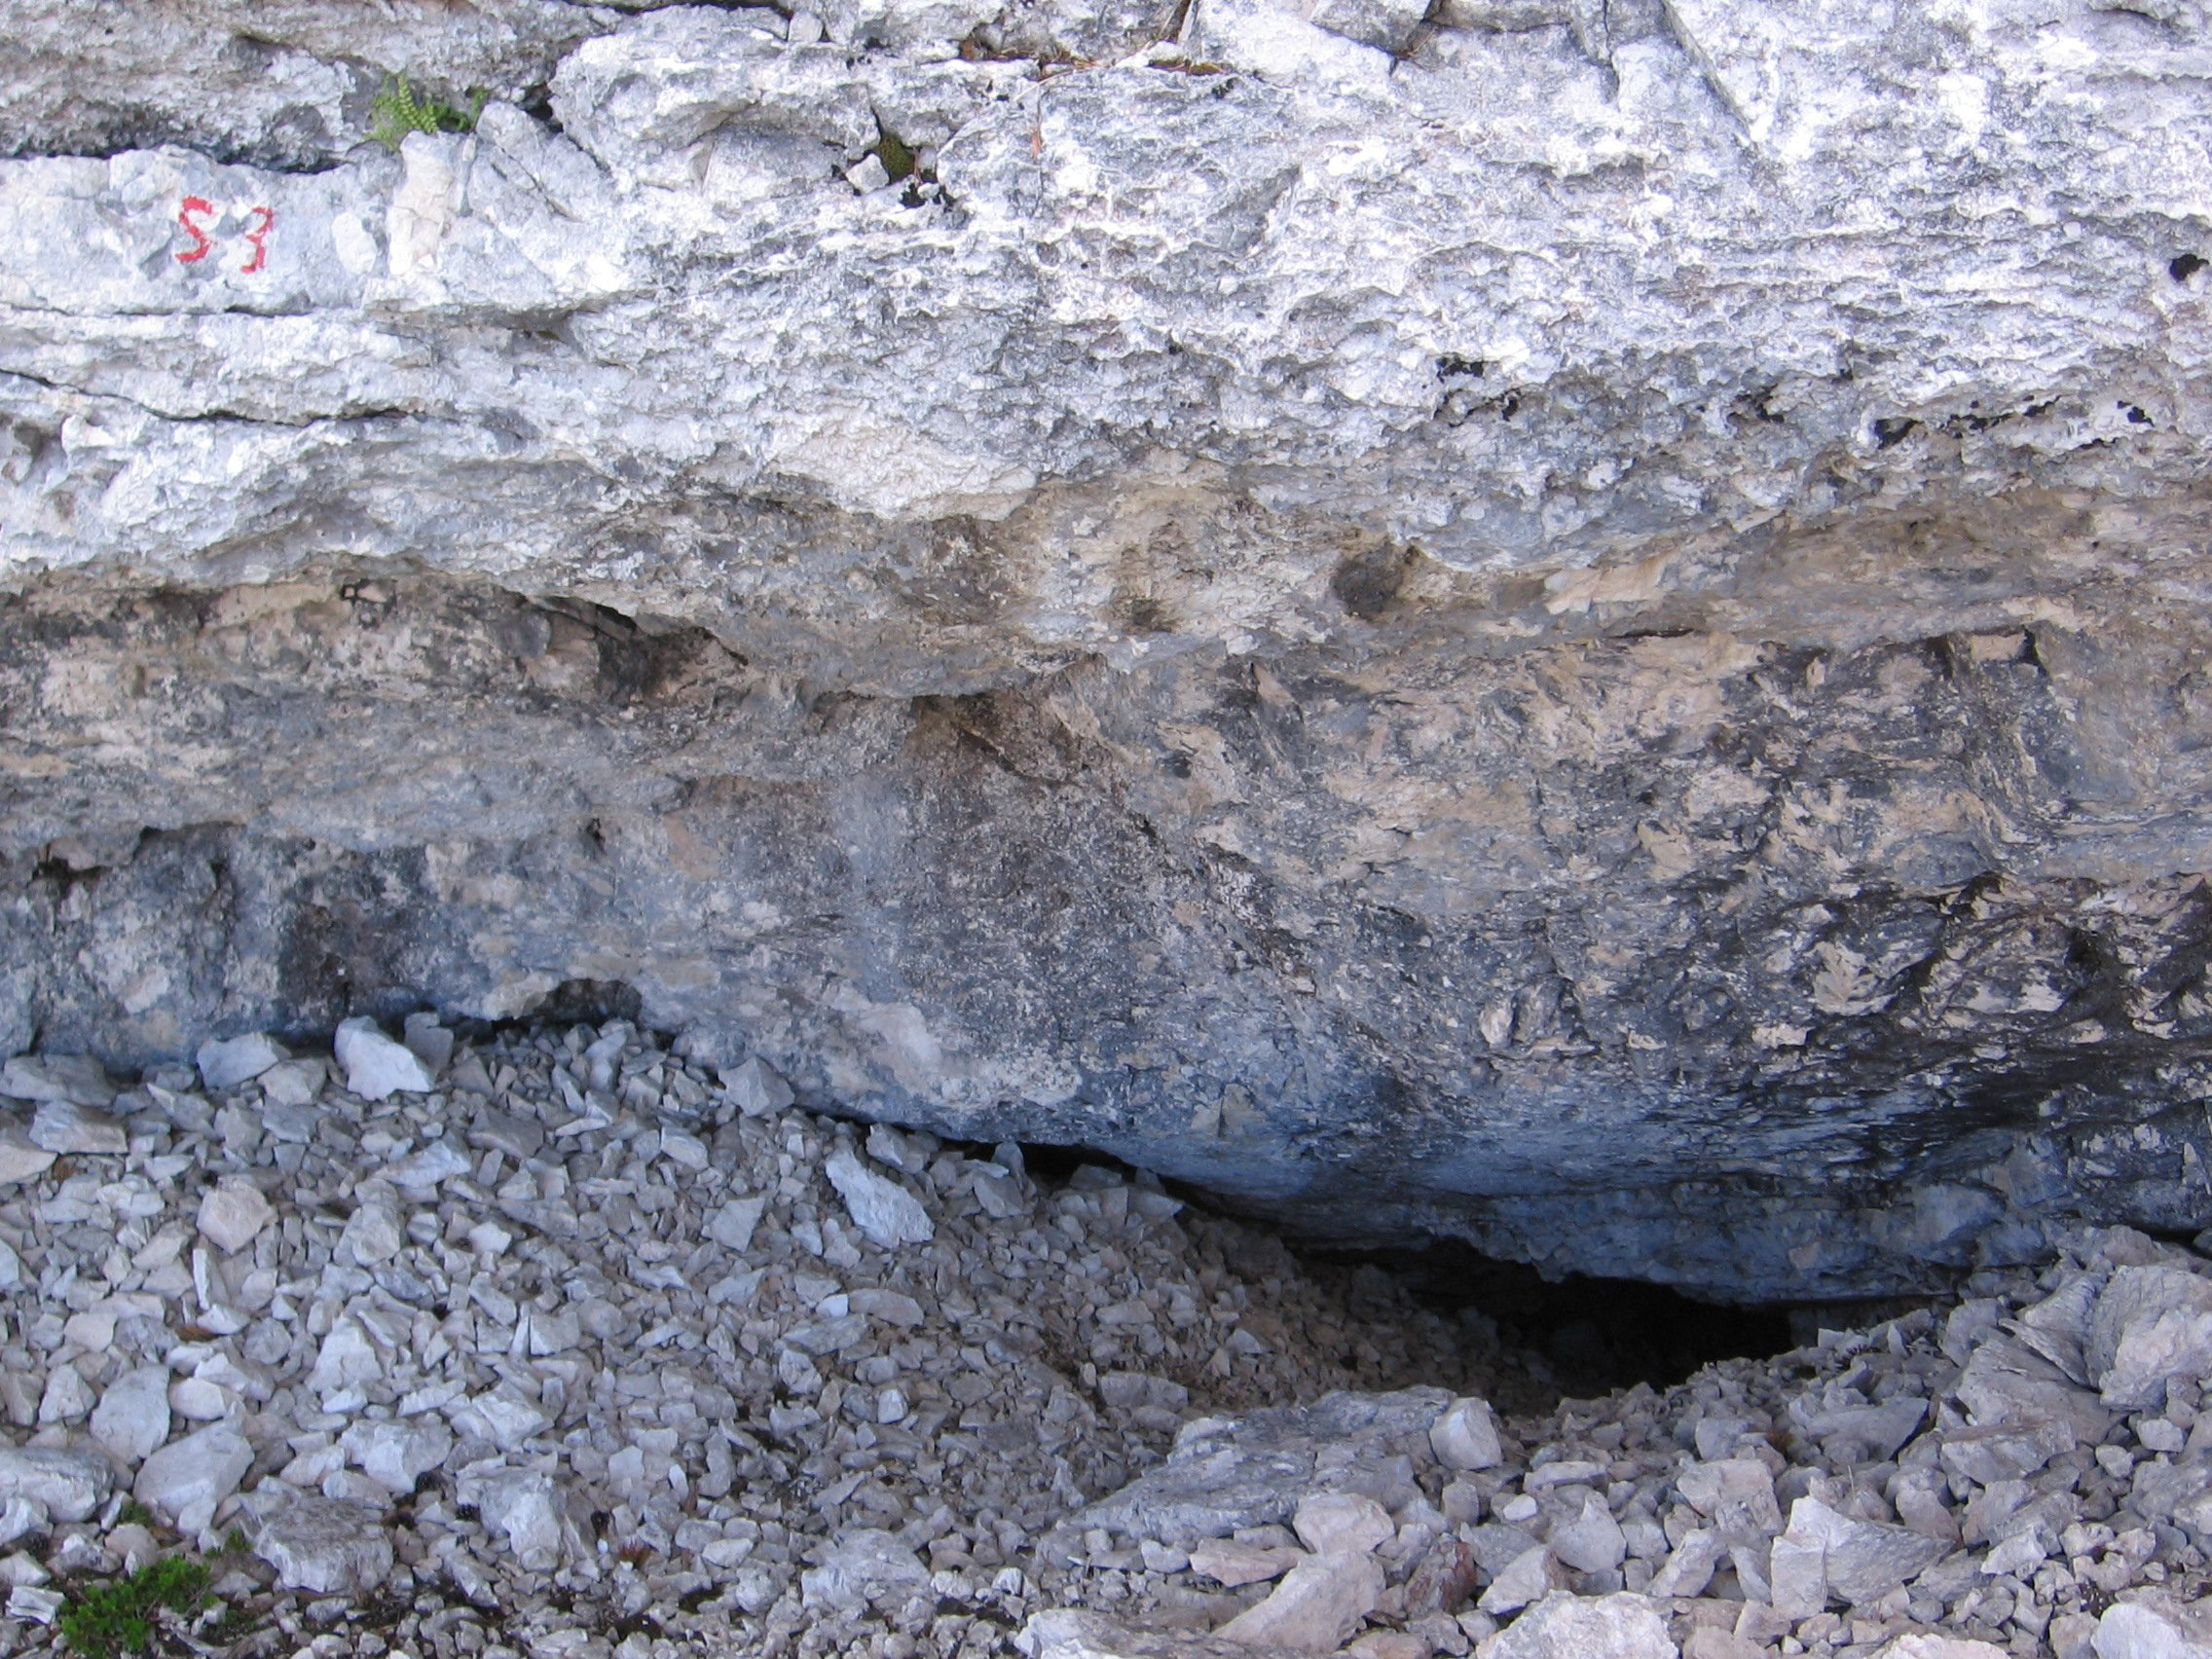
\includegraphics[width=\linewidth]{2007/S/jarvist frost - s3 entrance--orig.jpg}}
        \caption{\protect\passage{S3}}
\end{subfigure}
\vfill
\begin{subfigure}{0.49\textwidth}
    \centering
        \frame{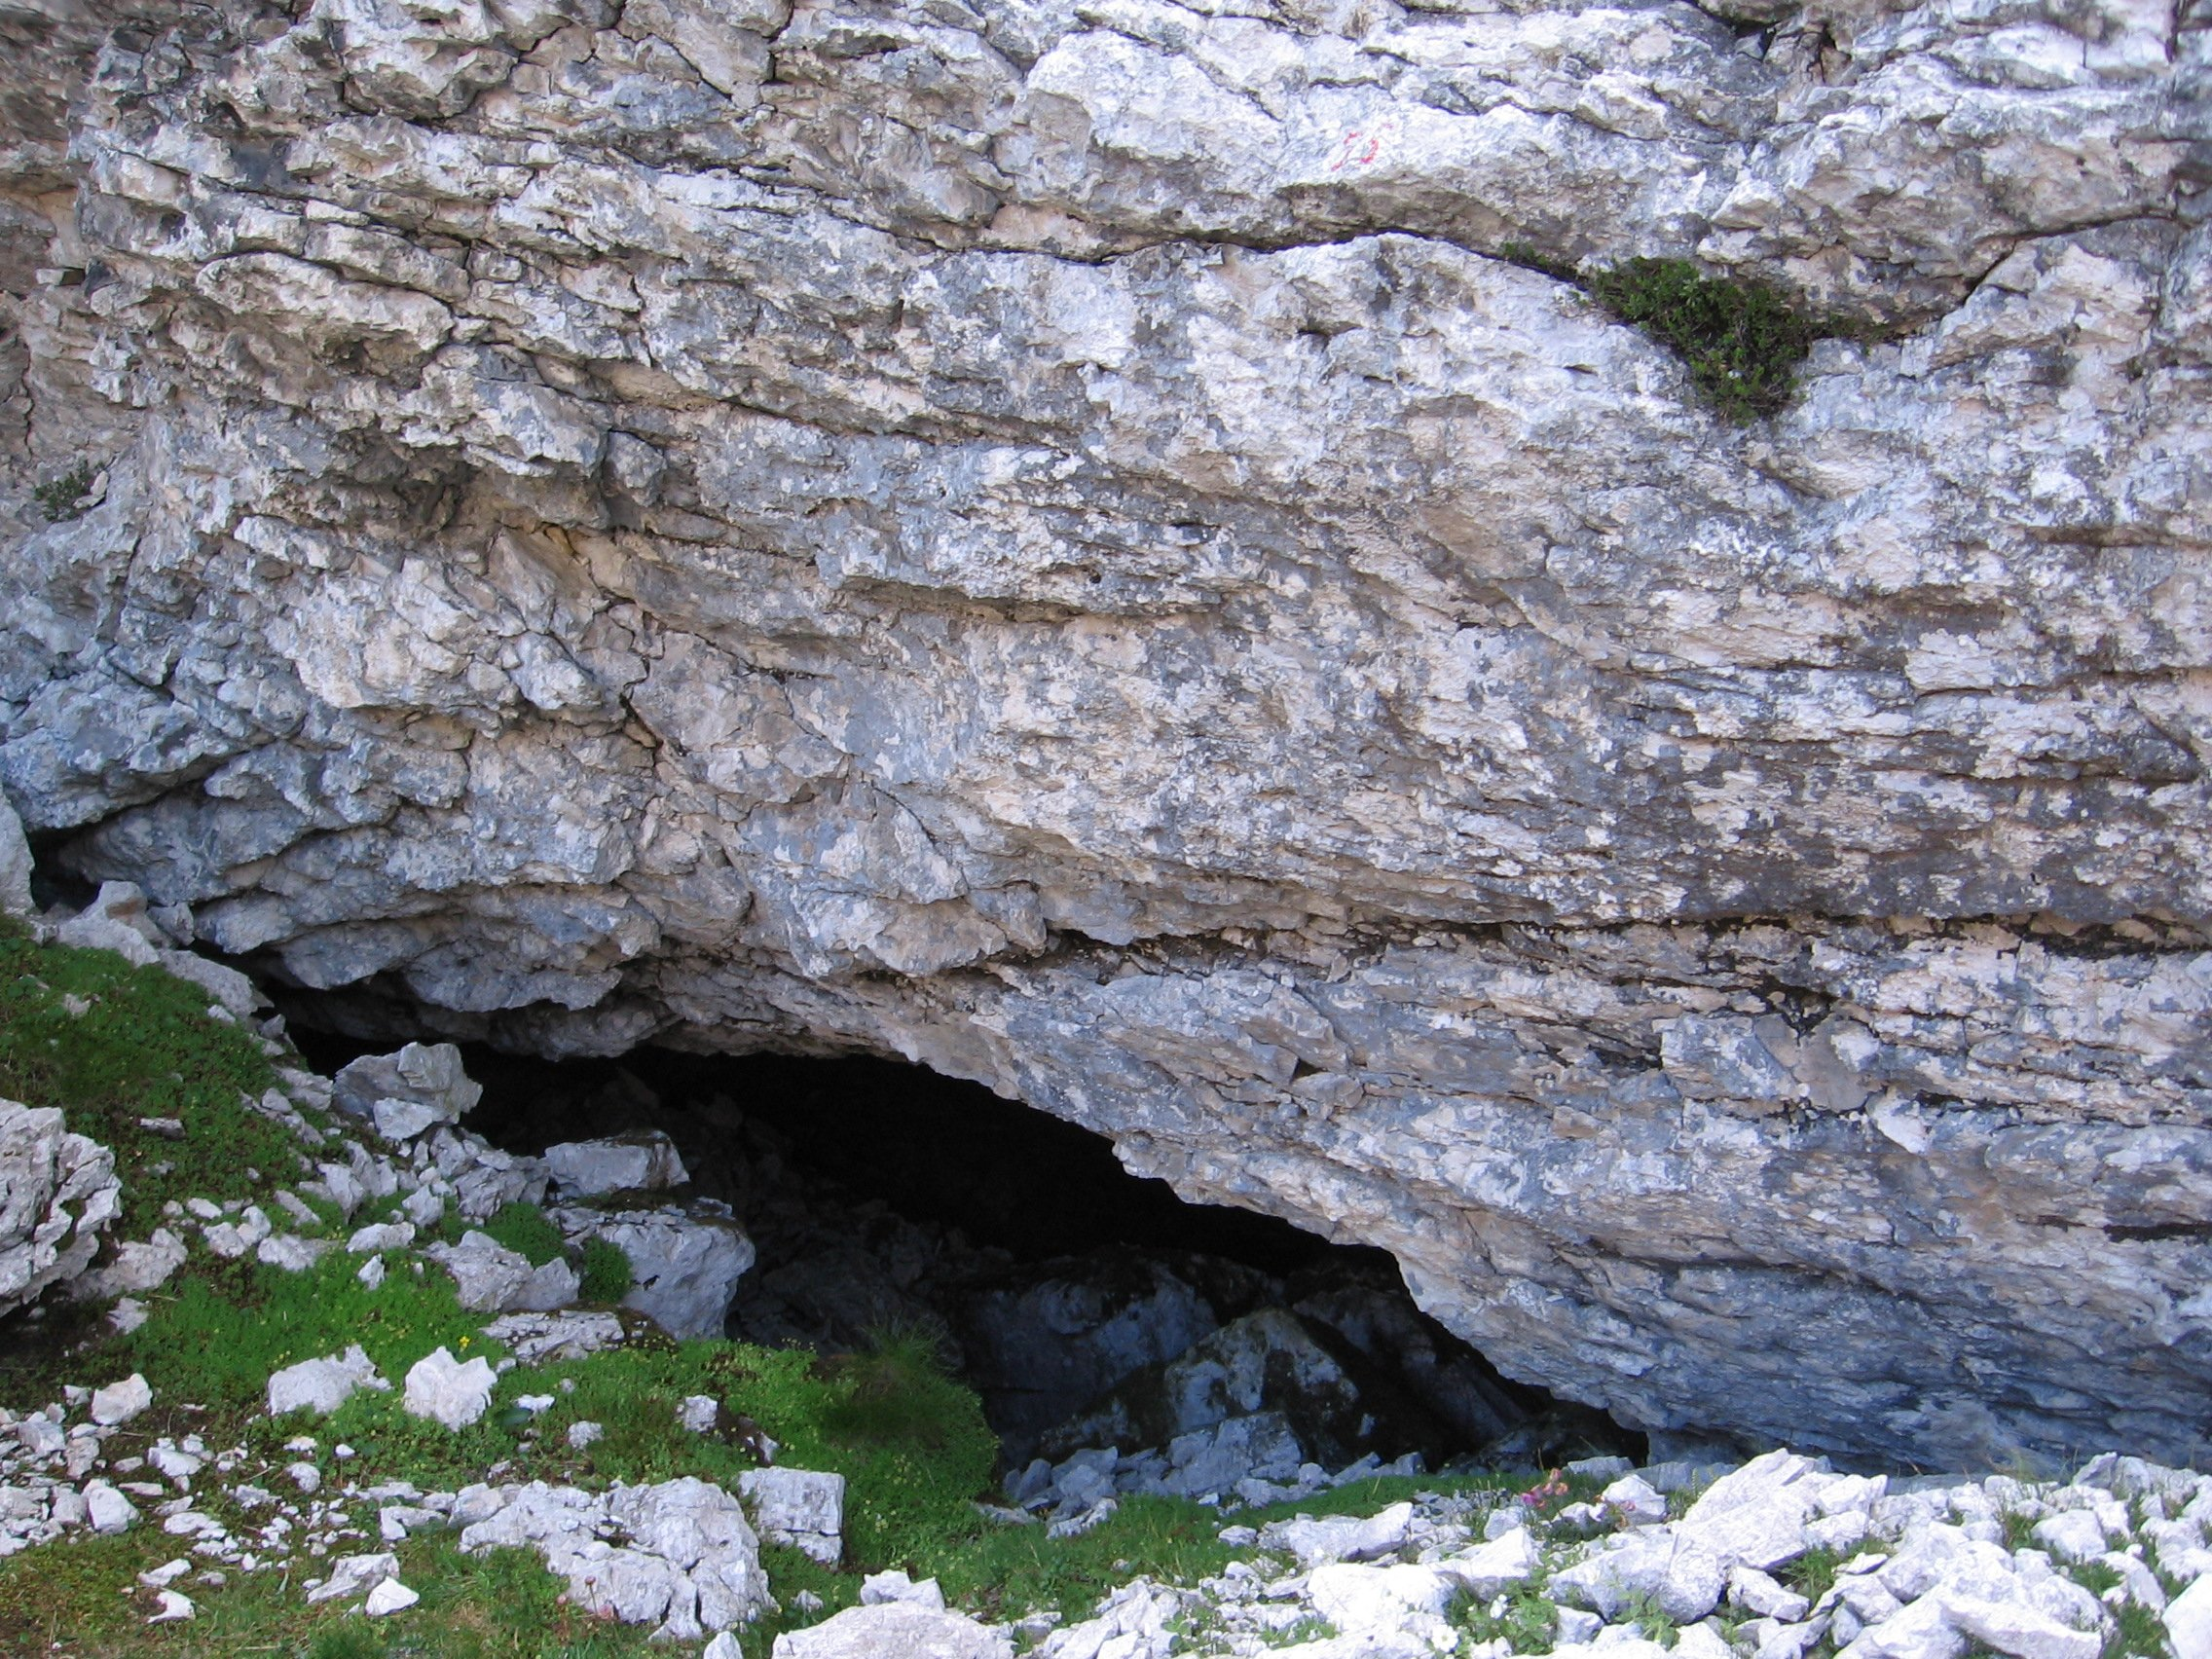
\includegraphics[width=\linewidth]{2007/S/jarvist frost - s5 entrance--orig.jpg}}
        \caption{\protect\passage{S5}}
\end{subfigure}
\hfill
\begin{subfigure}{0.49\textwidth}
    \centering
        \frame{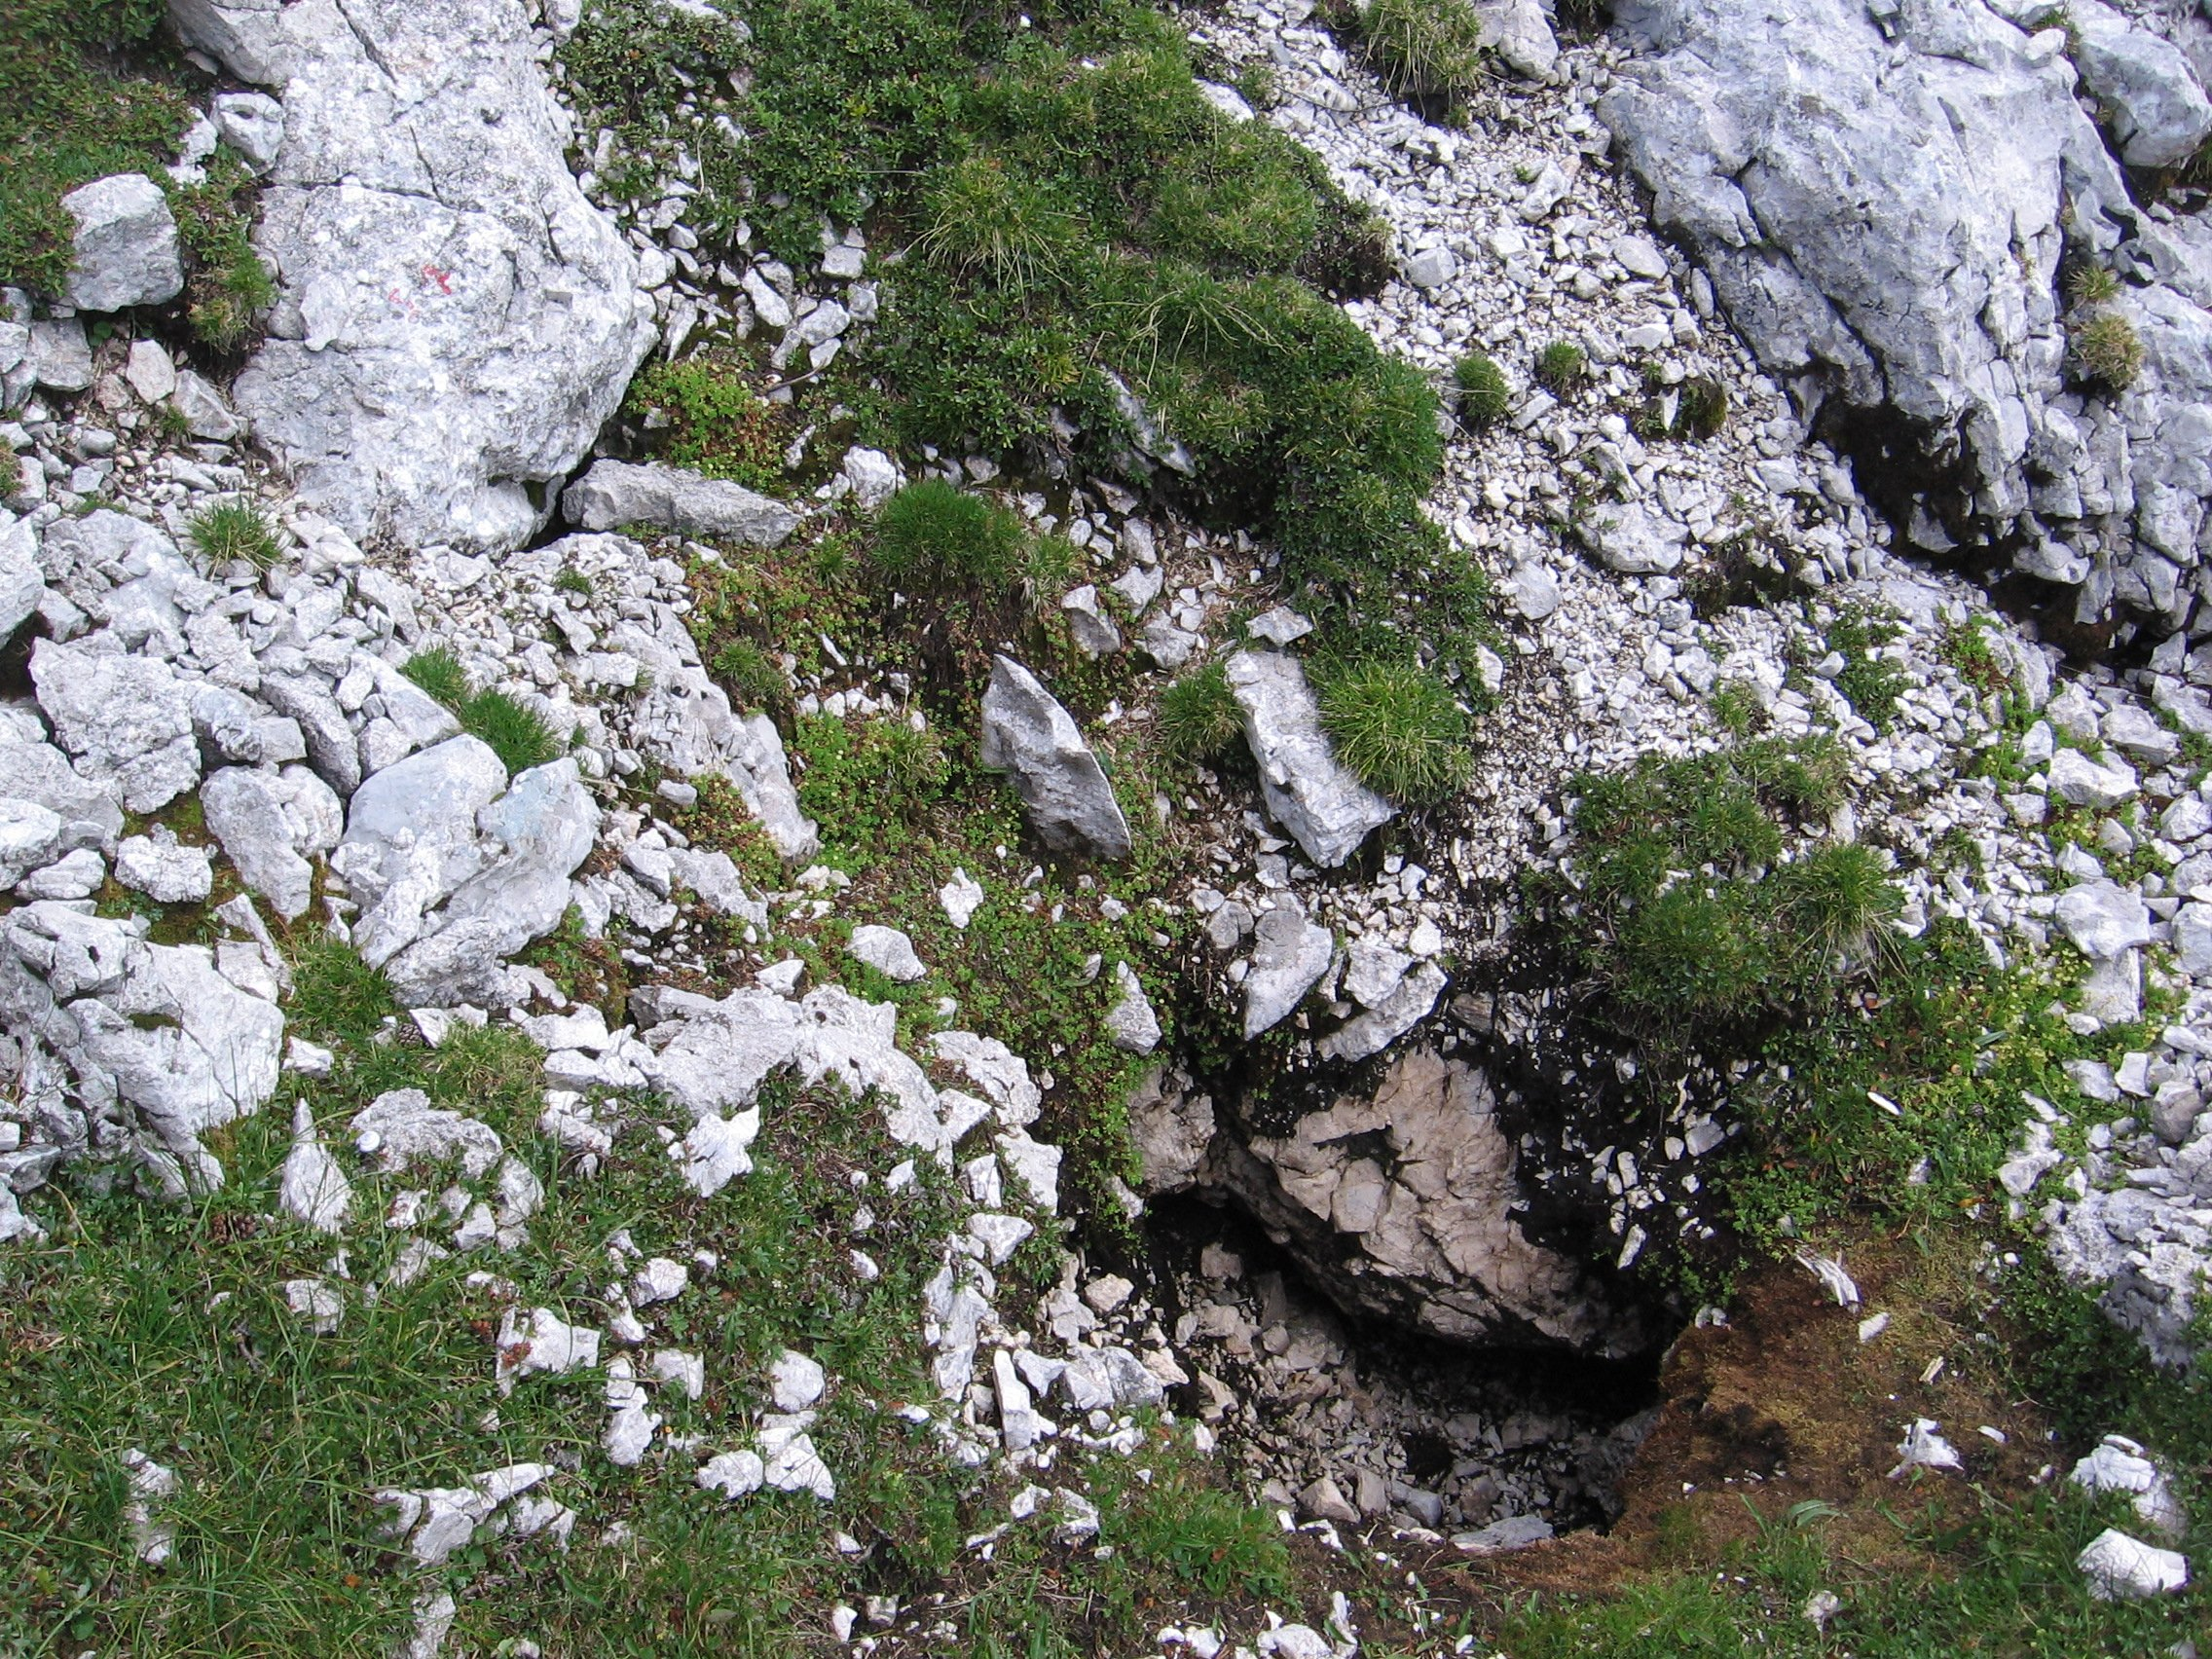
\includegraphics[width=\linewidth]{2007/S/jarvist frost - s7 entrance--orig.jpg}}
        \caption{\protect\passage{S7}}
    \end{subfigure}
\caption{Some of the entrances of the lesser-known holes in the S-series. \pic{Jarvist Frost}}
\end{pagefigure}



After a jolly into \passage{System Migovec} earlier in the week in a large group,
it was definitely time for me to go deep in a pair. What better way than
to help Rik push \passage{Captain Kangaroo}! With leads that had been looked at
but not surveyed, interesting data collection in scrott was the order of
the day. Down, down, down through the early \passage{Gardeners' World} pitches and
past some ``interesting'' rigging (greatly improved later in the
expedition). Squiggling through the rifts in \passage{Scrotty} until we reached
\passage{Traverse Chamber}. The first lead ended quickly in a pitch preceded by a
tight squeeze past a spiney. With no rope and no hammer to help make the
entrance more accessible let alone rigging, it was impossible for now.
After surveying back to a fork, we pushed on.

What followed was a crash course in free climbing as taught by Rik.
Plenty of top tips later, we made it past the fiddly squeeze where Rik
and Jarvist turned back at the last exploration. Beyond was an open
chamber. Rik climbed down and \bignote{suddenly \passage{Captain Kangaroo} became a whole
lot more exciting}. A pitch, two going rifts and horizontal walking
passage. The climb was do-able, but really needed rigging, so we turned
and surveyed back to \passage{Traverse Chamber}. Out an hour early, we hurried
back to camp for slop. As our survey data, excitement mounted. Our data
was heading towards \passage{System Migovec} for the mythical connection. The
laptop was whipped out and data entered. Our survey came within 36 m of
the bottom \passage{M2} below \passage{Silos}! A bit of rope and some further pushing
and we'll be there. Roll on the survey legs!

I found the expedition an extremely enjoyable and fulfilling experience.
I gained a lot of valuable caving experience. The exploration and
discovery of new cave passage was very rewarding. Having my waist freed
from wearing a battery belt, made caving in tight passageway and
squeezes immeasurably easier. I would like to thank the Ghar Parau
Foundation and the Alex Pitcher Memorial Fund for helping me on my first
caving expedition.

\name{Ben Banfield}


\section{Ping Pong Ball Bombe}

\margininbox{Smer0}{
     \begin{itemize}
    \item Aljošha Bončina
    \item Erik Bončina
    \item Emil Frankič
    \item Jarvist Frost
    \item Iztok Možir
    \item Zdenko Rejec
    \item Richard Venn
    \item Silan    
    \end{itemize}}{\explo}


A Slovene super-action was in the making, the Shepherd's huts stocked
with drink and the young JSPDT bouncing down to -200 m in
\passage{Primadona} to improve the rigging. The plan was to (mainly)
investigate leads off \passage{Smer0}/\passage{Smer1} in \passage{Primadona} where on a JSPDT
trip in Autumn 2006 (joined by Tetley \& Jarv from IC) a large rift with
an approx 40 m pitch was found - most tellingly, with water visible at
the bottom. Finding a constant stream this shallow in \passage{Mig} was unheard
of. Meanwhile, a smaller team would head to \passage{Bikini Carwash} at the
end of \passage{Exhibition Road} in the main system and aid climb to see if the
passage continued.

The more curious aspect of this mission was the Ping Pong Ball Bombe, a
plan to take ping pong balls down \passage{Primadona} \& set fire to
them. The noxious smell hopefully providing a connection. Alas, the
\passage{Sistem Migovec} team that was to detect with their noses, also contained the most
hardened smokers who spent their time sniffing the air in between
dragging on filterless roll ups!

With mammoth organisation, Rik and Jarv were dispatched down via text
message from the \passage{Bivi} to \passage{Kal}, meeting the Slovs and stealing some bread
before crabbing across sideways to \passage{Primadona}. The boulder slope
climb was awful as ever, but I took the opportunity to build a cairn on
the edge of the cliff so that we could recognise this point from the
plateau - to help unravel the mystery of the caves below \passage{B9} spotted by
Jana \& I from the plateau the Autumn before.

So we went down in a mammoth party: Rik, Jarv, Erik, Aliosha, Izzy,
Silan, Zdenko \& Emil.

Zdenko led off with the young JSPDT. Emil was a new character to us --
with a bald head framed by round lensed glasses and a fine handlebar
moustache that dovetailed with his military demeanour, were it not for
the Slovene language I could have easily assumed him to be an old-school
English army Colonel. Bringing up the rear with Emil, we were slowed by
his enormous tackle sac, stuffed full of bread and cheese I could only
assume. About 150 m in, standing on a traverse line above a pitch, I was
handed a full mineral water bottle from the depths of this magic sack.
``What is it?'' I asked. ``Mmm\ldots{} made with fruits\ldots{} and a
kilo of Med (honey)\ldots{} it's dobra!'' Ah, I thought, some marvellous
mountain tea fortified with a shed load of honey - just perfect to give
an energy boost and fight off the dehydration. \bignote{I chugged it back. Tea it
was not. Double distilled Zjganja with a kilo of honey dissolved in it
it was}.

Once at the pushing front we found we were rather limited with gear --
just one bolt kit. Rik set to work with Izzy to get down the pitch.
Zdenko and the Eric/Aliosha brotherhood set off for the end of \passage{Smer0}
(passed where \passage{Smer1} reconnected to it) to look at the climb that
currently ended the passage. Jana, Emil \& myself traversed over the
pitch (which was a truly frightening undertaking - walls over a metre
apart with a 40 m drop down) and went to look at where the water which
trickled down the opposite side came from. From the pools of water we
found a 2 m climb into an old dry silted phreatic system leading left
facing towards the end of \passage{Smer0}, starting just before where \passage{Smer1}
dropped down. This branched to a small chamber with avens, a too tight
rift (from which, insanely enough, emanated sounds of Rik bolting) and a
chamber with a larger, aid climbable, aven. Alas, with no spare rigging
gear for the climb, and no survey instruments, there wasn't much more
for us to do but go back to Rik.

Rik \& co had made it down about 20 m to a ledge where he put in a
rebelay bolt. He reckoned he could see the floor a further 20 m from
there. He was rather put off by the avalanche of rocks that came down
when people went over the crazy free traverse. The team that went to the
end of \passage{Smer0} was already back, and getting cold waiting around with
nothing to do we set off out in small groups. Rik finished the rebelay
bolt and headed back up, as the guys he was with were getting cold.

In the end we didn't burn the Ping Pong Bombes, as \passage{Primadona}
appeared to be breathing `out' in all the bits a draught was detectable.

As well as the spirits, Emil had another mineral water bottle filled
with white wine, for the journey out. When he returned to the mountain
hut well gone midnight he did not look particularly well. \bignote{One can only
assume he burnt through his hangover on the pitches out}!

\passage{Primadona} is I'm sure an absolutely amazing cave system, whose
secrets have only been very partially unlocked. Unfortunately I fear it
will require a heroic effort to make easier access (possibly by
reactivating the abseil route, or finding a better abseil way down via
\passage{B9}/\passage{Planika}/\passage{Monatip}) to allow the dozens of small trips necessary to
properly relearn the cave system, recapturing the knowledge lost with
the retirement from caving of the `middle-aged' JSPDT who mainly
explored \passage{Primadona}.

\name{Jarvist Frost}


\begin{pagefigure}
      \checkoddpage \ifoddpage \forcerectofloat \else \forceversofloat \fi
      \centering
              \frame{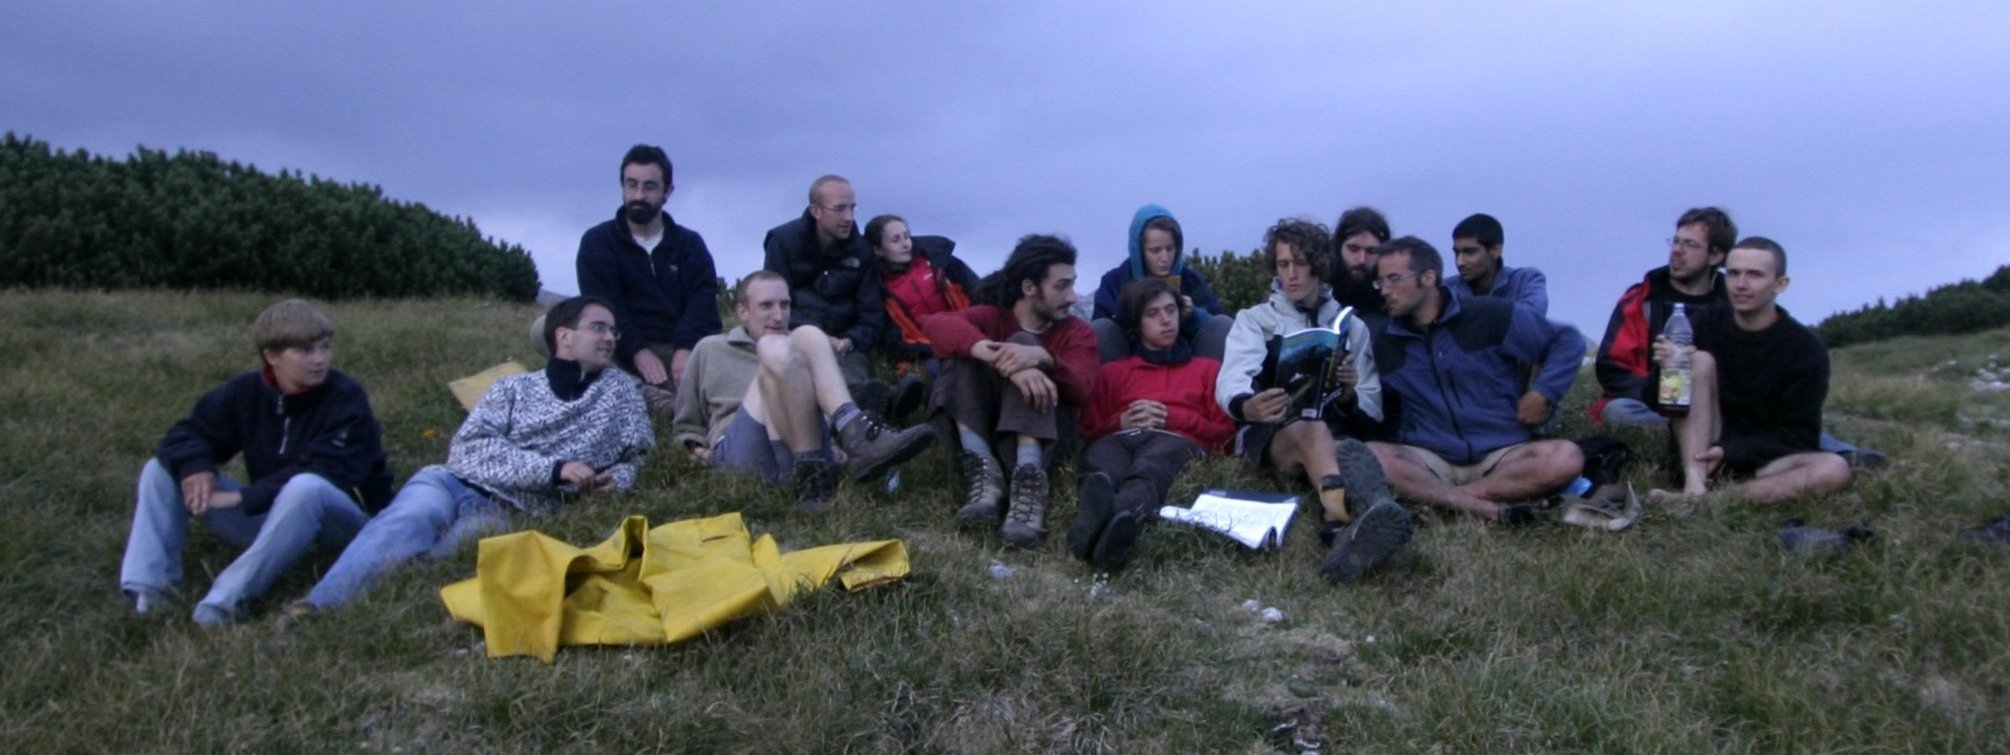
\includegraphics[width=\linewidth]{2007/ping_pong_ball_bombe/martin mcgowan -sunset shot--crop.jpg}} 
  \caption{Jarv gives a 'Sermon on the Mount', \passage{Migovec} style, by reading from \textit{The Hollow Mountain} (published 2007) to the masses. \pic{Martin McGowan}}
\end{pagefigure}


\section{B9 \& Beyond! - Planika Jama}

\begin{marginfigure}
      \checkoddpage \ifoddpage \forcerectofloat \else \forceversofloat \fi
      \centering
              \frame{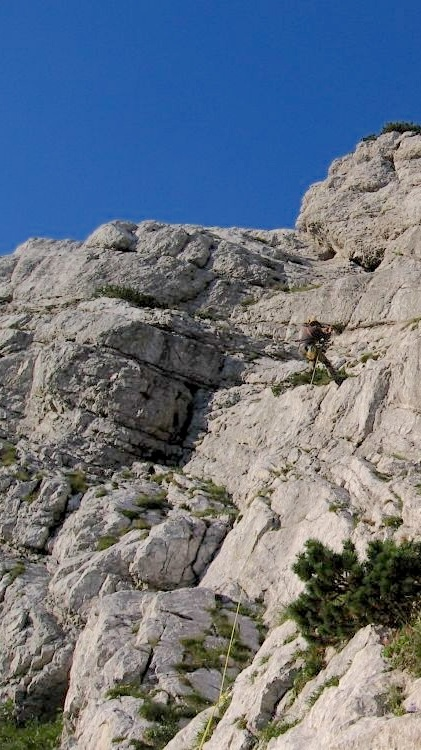
\includegraphics[width=\linewidth]{2007/b9/jana carga - planika - cliff abseil--orig.jpg}} 
  \caption{The \passage{Planika} cliff abseil. \pic{Jana Čarga}}
\end{marginfigure}

\margininbox{B9}{
     \begin{itemize}
    \item Aljošha Bončina
    \item Špela Leban
    \end{itemize}}{\explo}

Walking briefly over to \passage{B9} the day after the super-action, we could spot
the cairn I left down near \passage{Primadona}. Combined with one placed by
Jana \& I on the headland near \passage{U-Bend}, suddenly the whole complicated 3D
structure fell into place. Neither of the caves we could see from near
B9 were \passage{Primadona}, though the entrances looked similar - both
were new caves in an area never visited!

The next day we were joined on the plateau by some of the young JSPDT.
Jana \& I went with Alijosha and Spela to \passage{B9}, and explained the
situation. The weather was awful - thick cloud everywhere. While the
Slovs re-explored bits of \passage{B9} and checked to see if anything had changed
after the earthquake\sidenote {occurred 1998 \& 2004} (a pitch had disappeared off the original survey as
a bit of the cave collapsed and turned into a boulder climb!), I placed
two bolts for the descent down the cliff. This was really quite
exhilarating - a gale swept over the edge of the plateau, the rock was
soaked and slippery, and every now and then the thick clouds would part
for a glimpse of \passage[mountain]{Krn} or the \passage[river]{Tolminka} valley a very long way away!

The next day Aliosja and Spela went down from the plateau, so Jana and I
went back alone to \passage{B9} to rig down the cliff. The weather was much
improved! Jana abseiled down first and went investigating the three cave
entrances, while I came down behind and put in the rebelay bolts. The
three entrances were very interesting - the main one contained an
enormous aven which connected back up to the headland above \passage{U-Bend} (you
could see the sky through the top), but was an enormously steep boulder
slope with useless rock. The further entrance was a crawl in boulders
that was only briefly pushed by Jana. The smallest, highest entrance was
the most immediately interesting - a perfect metre by metre triangular
arch which led directly to a deep pitch. 

A shimmer of white was just
visible at the bottom. Bolts were placed for a traverse along a
beautiful slab of limestone to save freeclimb on the steep bowl valley
edged with a cliff, and the main hang bolt + first rebelay was placed
for the small-cave pitch, finishing our 100 m rope. We decided to name
this new cave \passage{Planika} Jama, after the rare mountain flower that covers
the sun-kissed (\& adder infested!) slopes around \passage{B9}.

\begin{marginfigure}
      \checkoddpage \ifoddpage \forcerectofloat \else \forceversofloat \fi
      \centering
              \frame{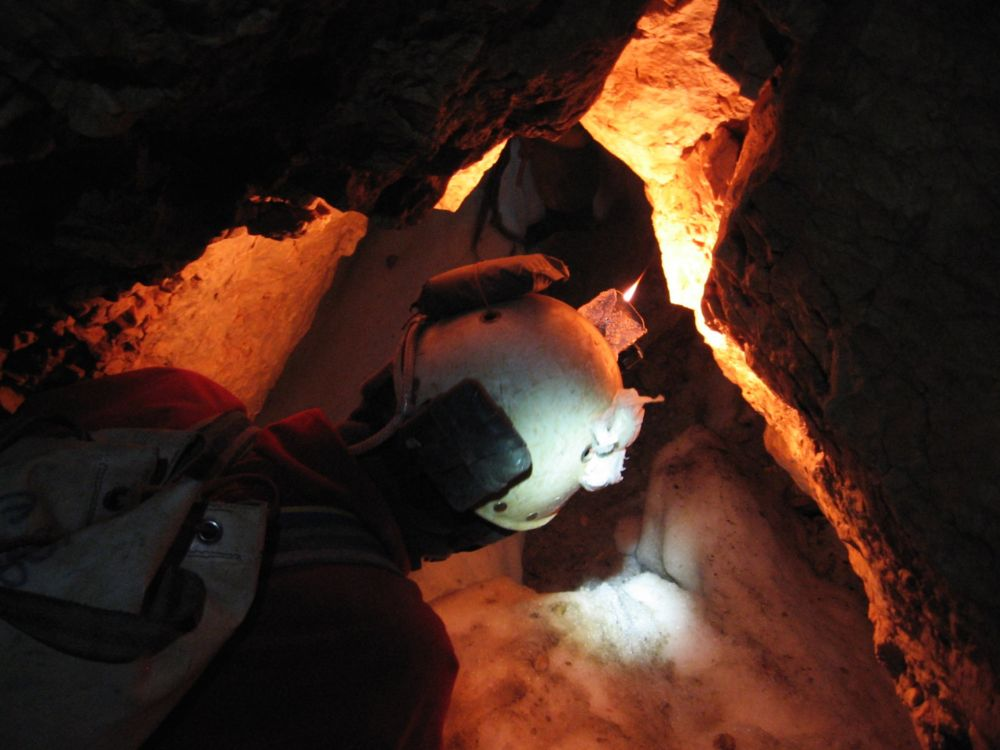
\includegraphics[width=\linewidth]{2007/b9/jarvist frost - planika - rock arch--orig.jpg}} 
  \caption{The triangular rock arch in \passage{Planika}. \pic{Jarvist Frost}}
\end{marginfigure}

Rather confusingly, we could occasionally hear echo-y shouts bouncing
around from below as we walked about the bowl valley, inevitably
disturbing stones. We tried to be as careful as we could, but couldn't
really understand what was going on - except for the fact that one of
the voices sounded like Kos.

Once back on the plateau, Jana pieced together the situation by mobile -
Alijosha and Spela had gone down to \passage{Kal}, taken the ICCC rigging gear
left in the third hut and went to the lower cave entrance pointed out to
them the day before via an abseil down the cliff near \passage{Primadona}
where I had placed the cairn on the Ping Pong Ball Bombe action. Jana
went down to \passage{Kal} to discuss the situation that evening and came back up
the next day rather upset. The new cave was to be called \passage{Monatip}
(`Fucking Idiot' in the local dialect).

\margininbox{Planika Jama}{
 \begin{itemize}
\item Jana Čarga
\item Jarvist Frost
\end{itemize}}{\explo}

\begin{marginfigure}
\centering 
  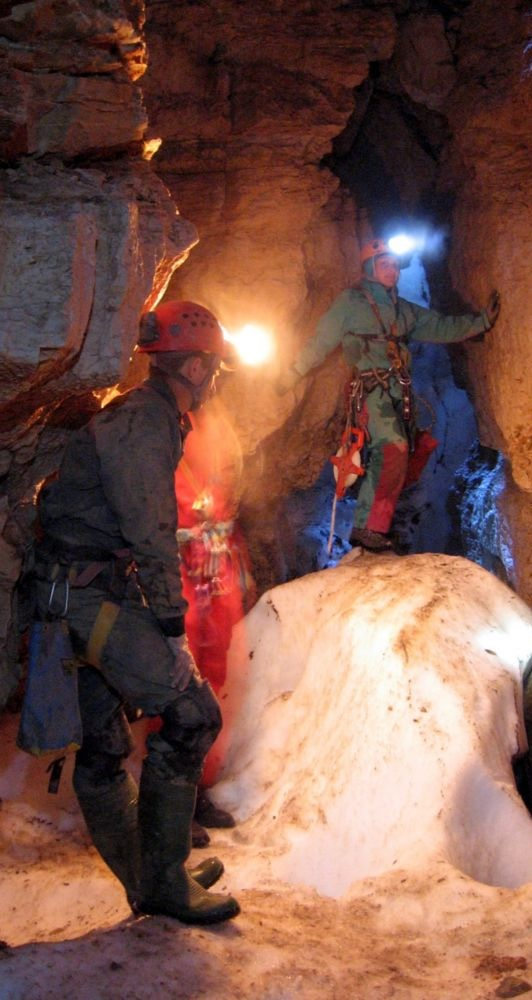
\includegraphics[width=\linewidth]{2007/b9/jarvist frost - planika - acre lane--orig.jpg}
  \caption{\passage{Acre Lane} in \passage{Planika Jama}. \pic{Jarvist Frost}}
\end{marginfigure}

The next day started with Goaty \& Jarv surface surveying to \passage{B9}. Jana
and I then descended the clif, surveying as we went. Again, within the
cave, we used the efficient technique of the lightweight Jana abseiling
down past rub-points, followed by Jarv bolting the rebelays behind while
Jana explored the next bit. The pitch was perhaps the most beautiful
entrance pitch on the Mig plateau. From a bolt placed in the ceiling a
hang dropped down past a fridge-sized boulder before swinging out to a
rebelay (placed by using my walking boot heel `skyhook'). 

From here one
abseiled down an almost perfect brick wall, above an enormous snow plug,
before swinging into a little dry streamway cascade to finish the last
bolt to land on the snow plug, which contained a large metre wide 6 m
deep hole bored out of the ice by wind or water, and similar, more
narrow, gaps on the edges of the plug. A small rift led off and
immediately closed down. 

From the top of the snow plug Jana found a
crawl way under a rock bridge to a climb up on ice on one side and rock
on the other (the ice was a more reliable foothold!), to reach a
snow-filled chamber which was daylight flooded and clearly below the
slope of the large entrance. An ice traverse in this chamber (we named
it \passage{Yorkshire Pudding}, as it was a torus of snow with a dimpled center).

From the far side of the Yorkshire pudding one could squeeze down
between the rock and snow, attempt a climb past a stack of wedged
boulders towards the aven, or walk down a snow-bottomed meander. The
meander we named \passage{Acre Lane} after our London home. This meander
suddenly regained a rock floor and led on to a tight rift which seemed
to be a small pitch head. There were a lot of boulders strewn around.
Here we PSS'ed and headed back.

The next day we were joined by Andreja \& James H. Jana and Andreja
bolted the backup bolt for this new traverse, while I gardened my way
along the tight rift and then placed a bolt holding myself in place
within the rift by breathing in until my ribs were wedged securely! This
was perhaps the slowest bolt I've every placed as I was lying sideways
with the arm holding the driver bent back behind my head, and the hammer
cocked under my buoy, while considering the 6 m drop to the floor! It
was with some relief that I took the rope through from the girls and
rebelayed my way down.

\margininbox{Planika Jama}{
     \begin{itemize}
    \item Jana Čarga
    \item Andreja Fratnik 
    \item Jarvist Frost
    \item James Huggett
    \end{itemize}}{\explo}

Around the corner the cave got strange once more - from a rock balcony
one is confronted with a chamber filled with a 45 degree slope of
compacted snow. Exploring around this we found that the upper levels
shut down, but seemed diggable (from the survey it appears that we were
within a metre of the Yorkshire Pud - it must be the same snow slope),
and there was a beautiful inlet which had formed some amazing
ice-pearls. 

The obviously way on was down. The snow steepened and
disappeared down at about 60 degrees with the rock roof not too far
away. Carefully traversing across the snow, I placed a bolt on the wall,
and abseiled down on my back. The ceiling closed in and the rope began
to rub, the walls shut down from both sides. At the bottom I faced the
end of the snow, with a 50cm gap of boulders sitting there.

\begin{marginfigure}
\checkoddpage \ifoddpage \forcerectofloat \else \forceversofloat \fi
\centering
 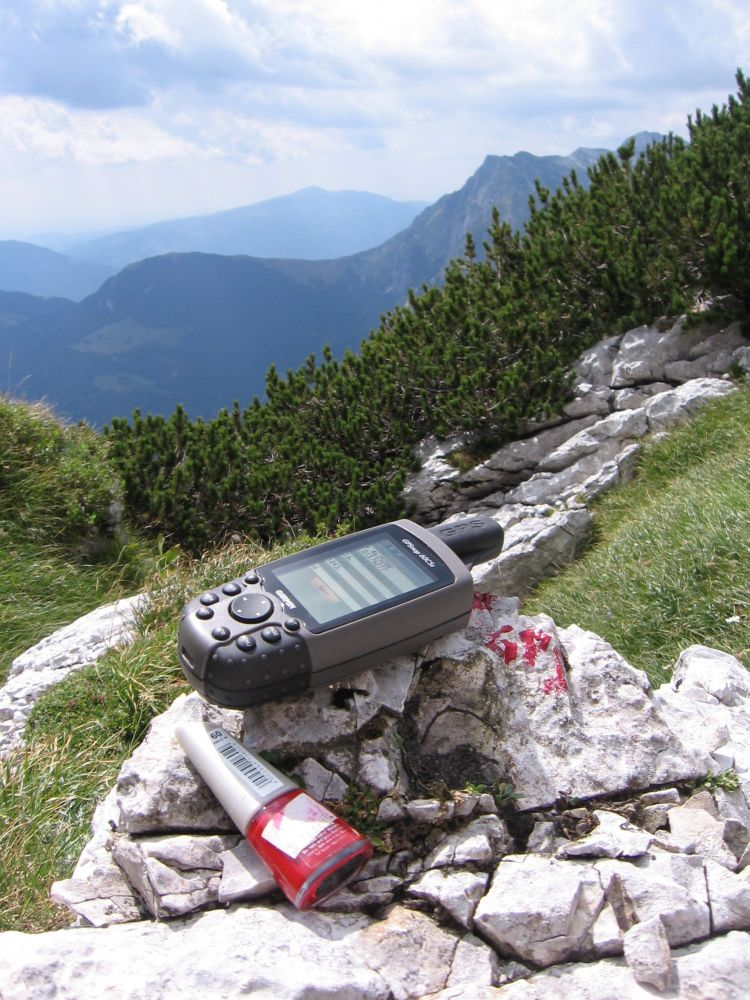
\includegraphics[width=\linewidth]{2007/b9/jarvist frost - b9 boulder cairn gps--orig.jpg} 
 \caption{GPS on the B9 boulder cairn. \pic{Jarvist Frost}}
\end{marginfigure}


The next step was obvious as it was insane - digging at the bottom of a
funnel with a lot of loose rubbish above. By picking up the boulders and
rotating I found I could play tetris, the fitting pieces disappearing
with a gravely rush through the floor. There was a strong draft, what on
earth was I digging towards? With a terrifying series of rock booms and
human shouts almost directly above my head, I pushed myself into the
corner of the snow shoot and hoped for the best. It turned out that the
rift pitch head had been disrupted as someone passed rope through,
collapsing a drystone wall and sending a few hundred kilos of rocks
cascading down. Jana had just reached the rebelay bolt going up,
\bignote{narrowly avoiding being caught in the waterfall of limestone}.

Once I stopped hyperventilating, and accepted that no further boulders
were coming down, I carried on digging with bare (now bloodied hands)
with ten minutes of frantic energy, a way was found. Originally I was
digging alongside the snow, but as it opened up I found I could go
straight down and way. A 5 m climb on boulders took me down to the
strangest chamber I have ever been in. Still attached to the rope, I
stood on a metre wide ledge that ran alongside a wall of perfect white
ice. The ice was wet - drips were everywhere. The ledge continued and
narrowed, snaking alongside this berg. From the middle of the ledge I
saw the strangest sight of my life - a phreatic crawlway winding down at
45 degrees through the ice, distinctly blowing, and with a similar rock
ledge and wall visible on the other side. With no bolt kit and no
camera, I headed out to my shaken compatriots. I was frozen, as my
wellies and cuffs were now packed with snow, and everyone was a little
shaken after the collapse.

  \margininbox{Planika Jama}{
     \begin{itemize}
    \item Ben Banfield
    \item Jana Čarga
    \item Emil Frankič
    \item Jarvist Frost
    \end{itemize}}{\explo}

Our last trip was a speedy survey, photo and derig, with Ben B and Emil.
Jana went down the ice slope but didn't fancy the still unstable boulder
climb, so we surveyed from this edge. The photo-gear was too much of an
effort to get passed the tight rift-pitch. Ben placed his first bolt as
a safety traverse across the ice. After surveying back to above the rift
pitch, we switched to photography documenting the cave as we derigged
out with the rope and metalwork.

Emil and Ben headed back to the Bivi while Jana \& I bolted down with
the Planika rope to reach \passage{Monatip} in order for him \& Izzy to surface
and cave survey the following day. Glorious weather, we sat watching the
sun set behind \passage{Krn}, with the Venetian bay visible beyond.

\name{Jarvist Frost}

\begin{marginfigure}
      \checkoddpage \ifoddpage \forcerectofloat \else \forceversofloat \fi
      \centering
              \frame{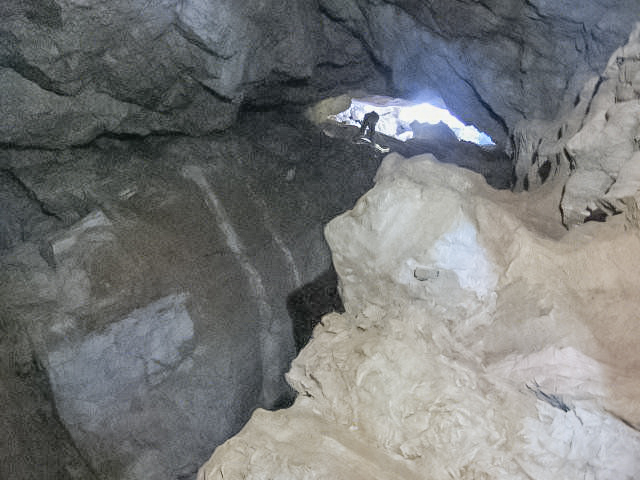
\includegraphics[width=\linewidth]{2007/b9/jarvist frost - planika - entrance pitch1--orig.jpg}} 
  \caption{The \passage{Planika} entrance pitch. \pic{Jarvist Frost}}
\end{marginfigure}

\newpage
\section{Notes on Photography}

\begin{marginfigure}
      \checkoddpage \ifoddpage \forcerectofloat \else \forceversofloat \fi
      \centering
              \frame{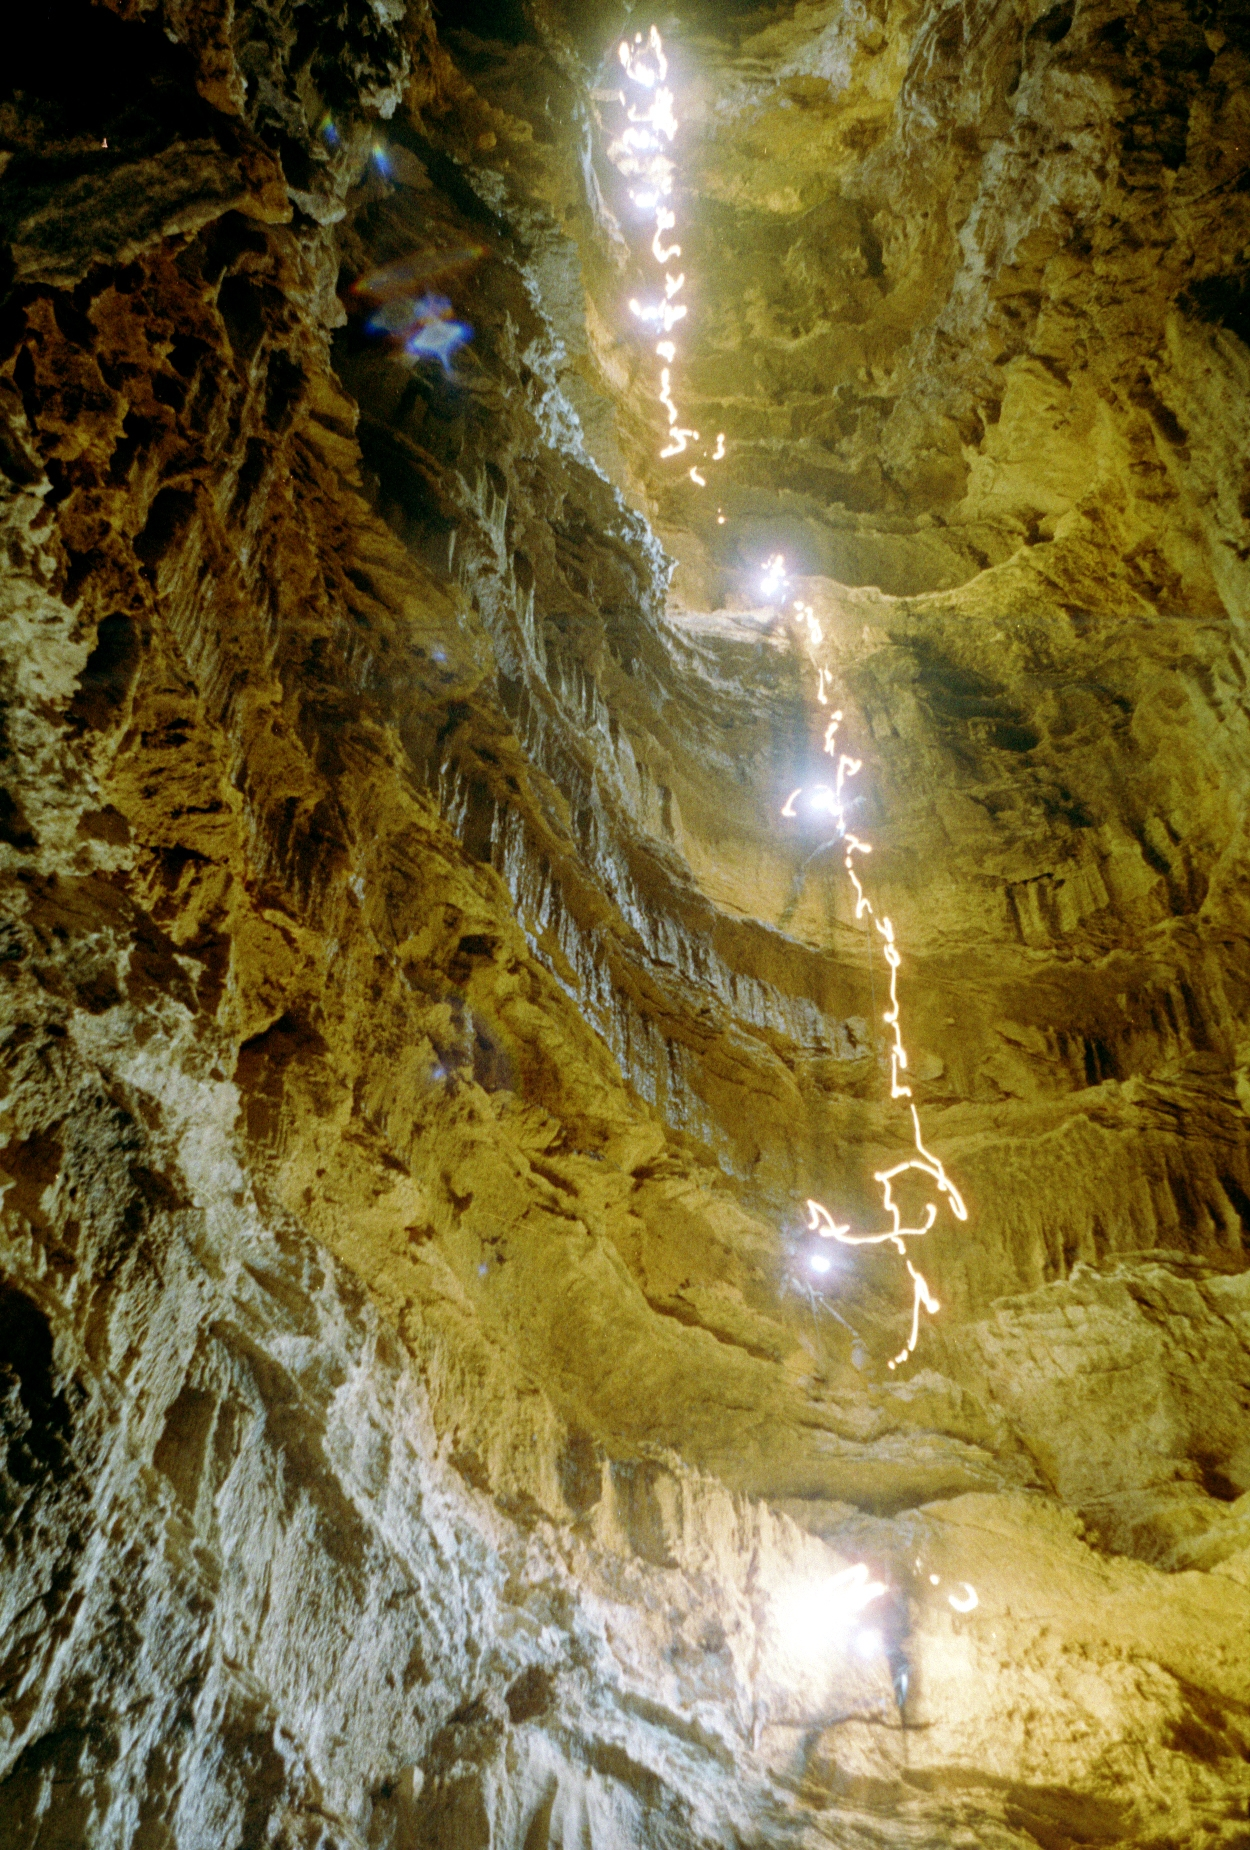
\includegraphics[width=\linewidth]{2007/b9/Clewin_on_Concorde_2004_Photo_by_Jarvist_Frost-highquality--orig.jpg}} 
  \caption{A long exposure shot of Clewin on \protect\passage{Concorde} pitch in \protect\passage{Vrtnarija}, taken in 2004. \pic{Jarvist Frost}}
\end{marginfigure}

\margininbox{That Concorde Photo}{

Zenit EM camera on Bulb (zenit's lock open without needing a seperate remote trigger) with a 49mm Helios lens (standard) at F4. Super cheap 200ASA Bonusprint colour-print film. Flash was fired every \textasciitilde 10 m, mostly at Rebelays and sometimes between. It was, I believe, one Jan's usual flashes, I think with a guide number of around 50. Total exposure was around 15minutes. £13 on eBay Zenit, £2 film, £5 developing - best £20 I've ever spent! \mininame{Jarv}}{\logbook}

\subsection{What Camera?}

Dave Wilson uses fully mechanical Rollei 35s, and has this to say: The 35LEDs take mercury batteries (PX27s?) for metering, which aren't obtainable these days, but there are some fixes available (from the Small Battery Company, I think). I have skylight filters on all the cameras to protect the lenses, and I think I have a couple of ND4s for surface shooting in bright light with fast film (the shutter only goes down to 1/500.

Jarv's cameras:

\begin{itemize}
    \item 35mm Ricoh GR1s/v. Bought from eBay for \textasciitilde£100 smackerones. Small enough to fit in my Peli 1030, and with a built-in timed exposure mode \& both infinite focus \& hyperfocal overrides, crystal perfect 28mm lens. Whoah. Took up mountain in lieu of SLR (Mig 2007) and was much impressed by quality of prints, less impressed by quality of digitisation from film.
    \item Zenit-E. Helios 49mm lens (see Concorde shot), and cheap 28mm F3.5 lens. So manual it hurts. Would probably survive nuclear war. Was quite possibly designed so.
    \item Canon AE-1, with 50mm SSC F1.4 lens and 28mm F3.5 lens. Have two bodies. Unfortunately design is one where the shutter is held open by battery power - so not so good for super super long exposure.
\end{itemize}

The spot-beam of miglights is strong enough to appear in photos as a rather sickly green spot; omni isn't generally strong enough. 


\subsection{Dealing with Noise}
Do you love noise? My Little A520 spews noise across the print. Best results involve the following GIMP flowchart:

    \begin{itemize}
        \item Speckle Reduction
        \item Gaussian blur with Pixel=1.6 (or more, if shot out of focus \& so not worsened by blurring)
        \item Unsharp mask with Pix\textasciitilde1.2 . Amount tuned for effect.
    \end{itemize}

Also: GREYCstoration is a FREE digital camera noise removal program, which both integrates into the GIMP \& as a stand alone utility. It's very very tunable.


\name{Jarvist Frost}


\begin{tcolorbox}
\chapter{2008 --- Votla Gora}

The main focus of the Votla Gora 2008 Expedition to the Tolminski
Migovec plateau, Western Slovenia, was the connection of Sistem Migovec
(11493 m - 5\(^{th}\) longest in Slovenia) with \emph{Vrtnarija} (5229 m
- 11\(^{th}\) longest) to make the second longest cave in Slovenia
(16722+m). The separation between the caves was 28 m on the centre line
with many going leads. This was not achieved, but 1.2 km of cave passage
was found and explored.

The part of Sistem Migovec that we were attempting to connect to was the
bottom of \emph{M2}, the original deep cave on Migovec pushed back in
the early 1970s by the Slovenian JSPDT. Below the epic \emph{Tolminski
Silos} pitch (P120 m), the cave shut down into a series of small pitches
with extremely tight rift, which had to be exploded open for passage.
Exploration finished in the 1970s at yet another such rift.

2008 was also the first ICCC Slovenia expedition with a name - `Votla
Gora', meaning `Hollow Mountain'. This was an idea, shamelessly copied
from the recent OUCC Ario Caves expeditions, which instantly became a
useful tradition.

\end{tcolorbox}
\backgroundsetup{
    scale=1,
    color=black,
    opacity=1,
    angle=0,
    contents={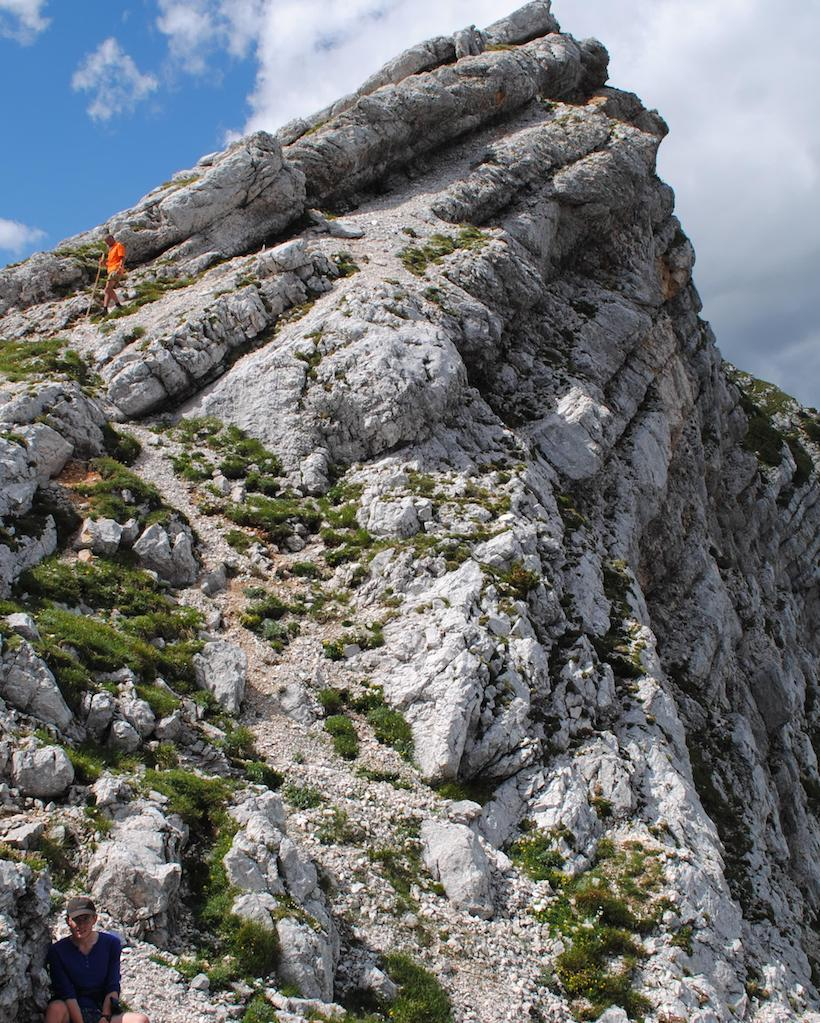
\includegraphics[height=\paperheight]{2007/intro/kuk-2013.jpg}}
}
\BgThispage










\section{The Summer Expedition Student Prospectus}

\textbf{Dates}: 12th July -> 17th August 2008 (5 weeks)

\tweet{7:54AM Jul 19th, 2008}{Belgium. Andy driving. Trance. Sunny. Three lanes. Van air a bit thick already. Shadows of rooftop barrels cast on tarmac.}

\textbf{Logistiscs}: We'll be taking the usual heavily-overladen 9-seater
minibus via the autobahn (1000miles), with spaces reserved for
Drivers and the Poor (undergrads). Everyone else to fly.
Base camp (where we park the bus) is at Ravne at 912m, the
Bivvi (mountain camp) is at 1850m or so: and all the cheese,
equipment, tents \& etc. needs to be carried up on our backs!

\subsection{Why on Earth would I want to do this?}

Many reasons! This is your opportunity to find something BIG, have an absolutely cracking summer a world away from [towm]London living in the wild battling with the rock and the storms above. If you've got any hunger for adventure, or a thirst to be first – you will not want to miss out on this.

Living on top of a mountain drinking snow melt is great fun (if at little stone-age sometimes), and we'll be
caving with the JSPDT. Eastern Europe's amazing and completely different to elsewhere – don't faff around
interrailing visiting Tourist traps, come and visit a country properly and learn the Slovene for “Cheese, Please, Yes, Please, Cheese!”

Also, you'd be joining in a very exciting year – the oft hypothesised connection between the two systems in almost unbearably close now, and you will have a serious chance of being there both at the big moment, and to bask in the glory afterwards!

\begin{pagefigure}
\checkoddpage \ifoddpage \forcerectofloat \else \forceversofloat \fi
\centering
\frame{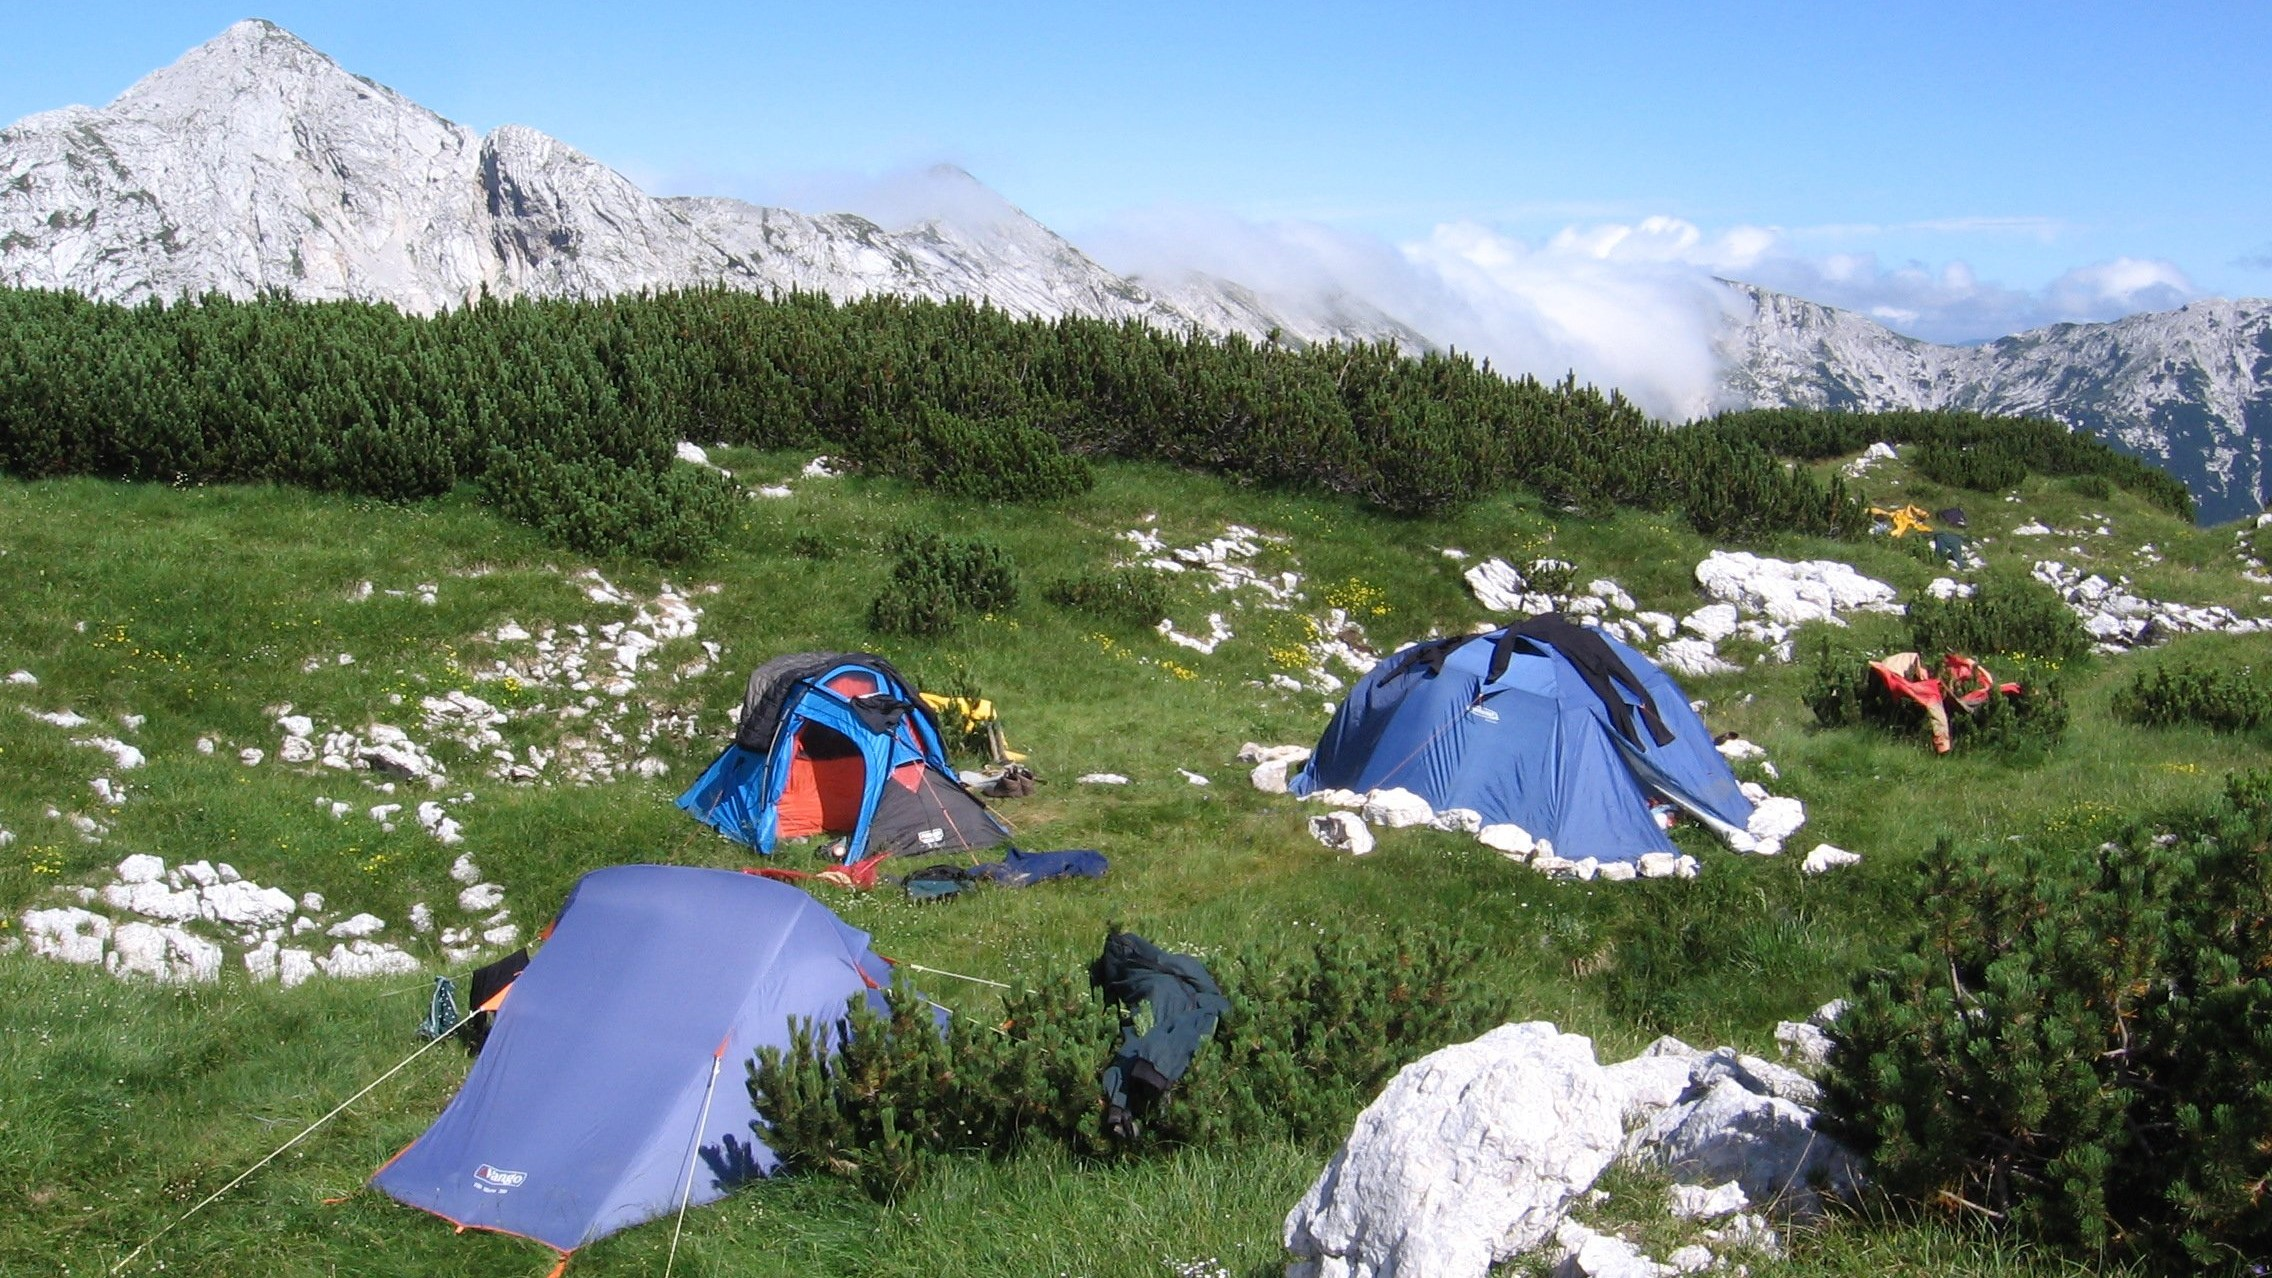
\includegraphics[width=\textwidth]{2008/why/Jarvist Frost - canon a520 - tents on plateau2--orig.jpg}}
\caption{A beautiful day on the \passage{Migovec plateau}. \pic{Jarvist Frost}} \label{tents}
\end{pagefigure}
\section{Expedition Findings}

\margininbox{Website announcement}{... Andreja reports from Migovec that there is still some snow in the bivi, rope is washed and prepped, Lidl has been abused, and the days are counting down... 
\mininame{Jarv}}{\logbook}

During the first two weeks of expedition, the UK team rebolted and
rerigged \passage{M2} via the original, more direct, entrance to the
original pushing point. Once there the UK team attacked the rift with
hammers and chisels, but the progress was slow. In the middle of the
expedition an experienced Slovenian caver with access to explosives came
on a trip at the same time as another team explored some of the near
passage in \passage{Vrtnarija}. This trip obliterated a large rock that was
blocking the rift, but also collapsed the wall of the rift. Net distance
gained - minus 50 cm! However, with another session of manual work the
choss was cleared. Perhaps worryingly, the extremely loud explosion was
not heard by the other party in \passage{Vrtnarija}, though one must add
that they were extensively `gardening' large rocks down the 52 m
\passage{Dangermouse} pitch!

\tweet{10:51PM Jul 14, 2008}{Union attempt to throw away 500m of new rope left soaking outside stores. Rescued from bins.}

Early exploration in \passage{Vrtnarija} was concerned with extending the
`bottom' end of \passage{Captain Kangaroo}. The first recce trip was over
12hrs in spite of no new rigging taking place, and concluded that
significant work was required just to improve the rigging and expand
some of the more arduous squeezes. In particular there were three tight
sections of rift in the \passage{Mudslump} extensions from 2007. As such,
the first few trips down to this area of the cave consisted of two
parties - an advanced one pushing the bottom end while the other
progressed slowly `improving' (in many cases instigating\ldots{})the
SRT rigging. For one notable pitch, \passage{Kill'em All}, which had
been rigged for no apparent reason without a traverse line, the advanced
party beckoned the clean-up group down to rig the pitch safely before
they would ascend!

After a section of acrobatic rift below \passage{Kill'em All} (P22 m),
\passage{Dark Tranquillity} (P42 m) was discovered. The leads were very much
ongoing - another pitch, and many windows. There were also entering
avens. However, on inputting the survey data (we have a solar-powered
laptop running Survex in our mountain top Bivi), we discovered that we
had dropped well below the bottom of \passage{M2} and therefore our current
connection possibilities.


\begin{marginfigure}
\frame{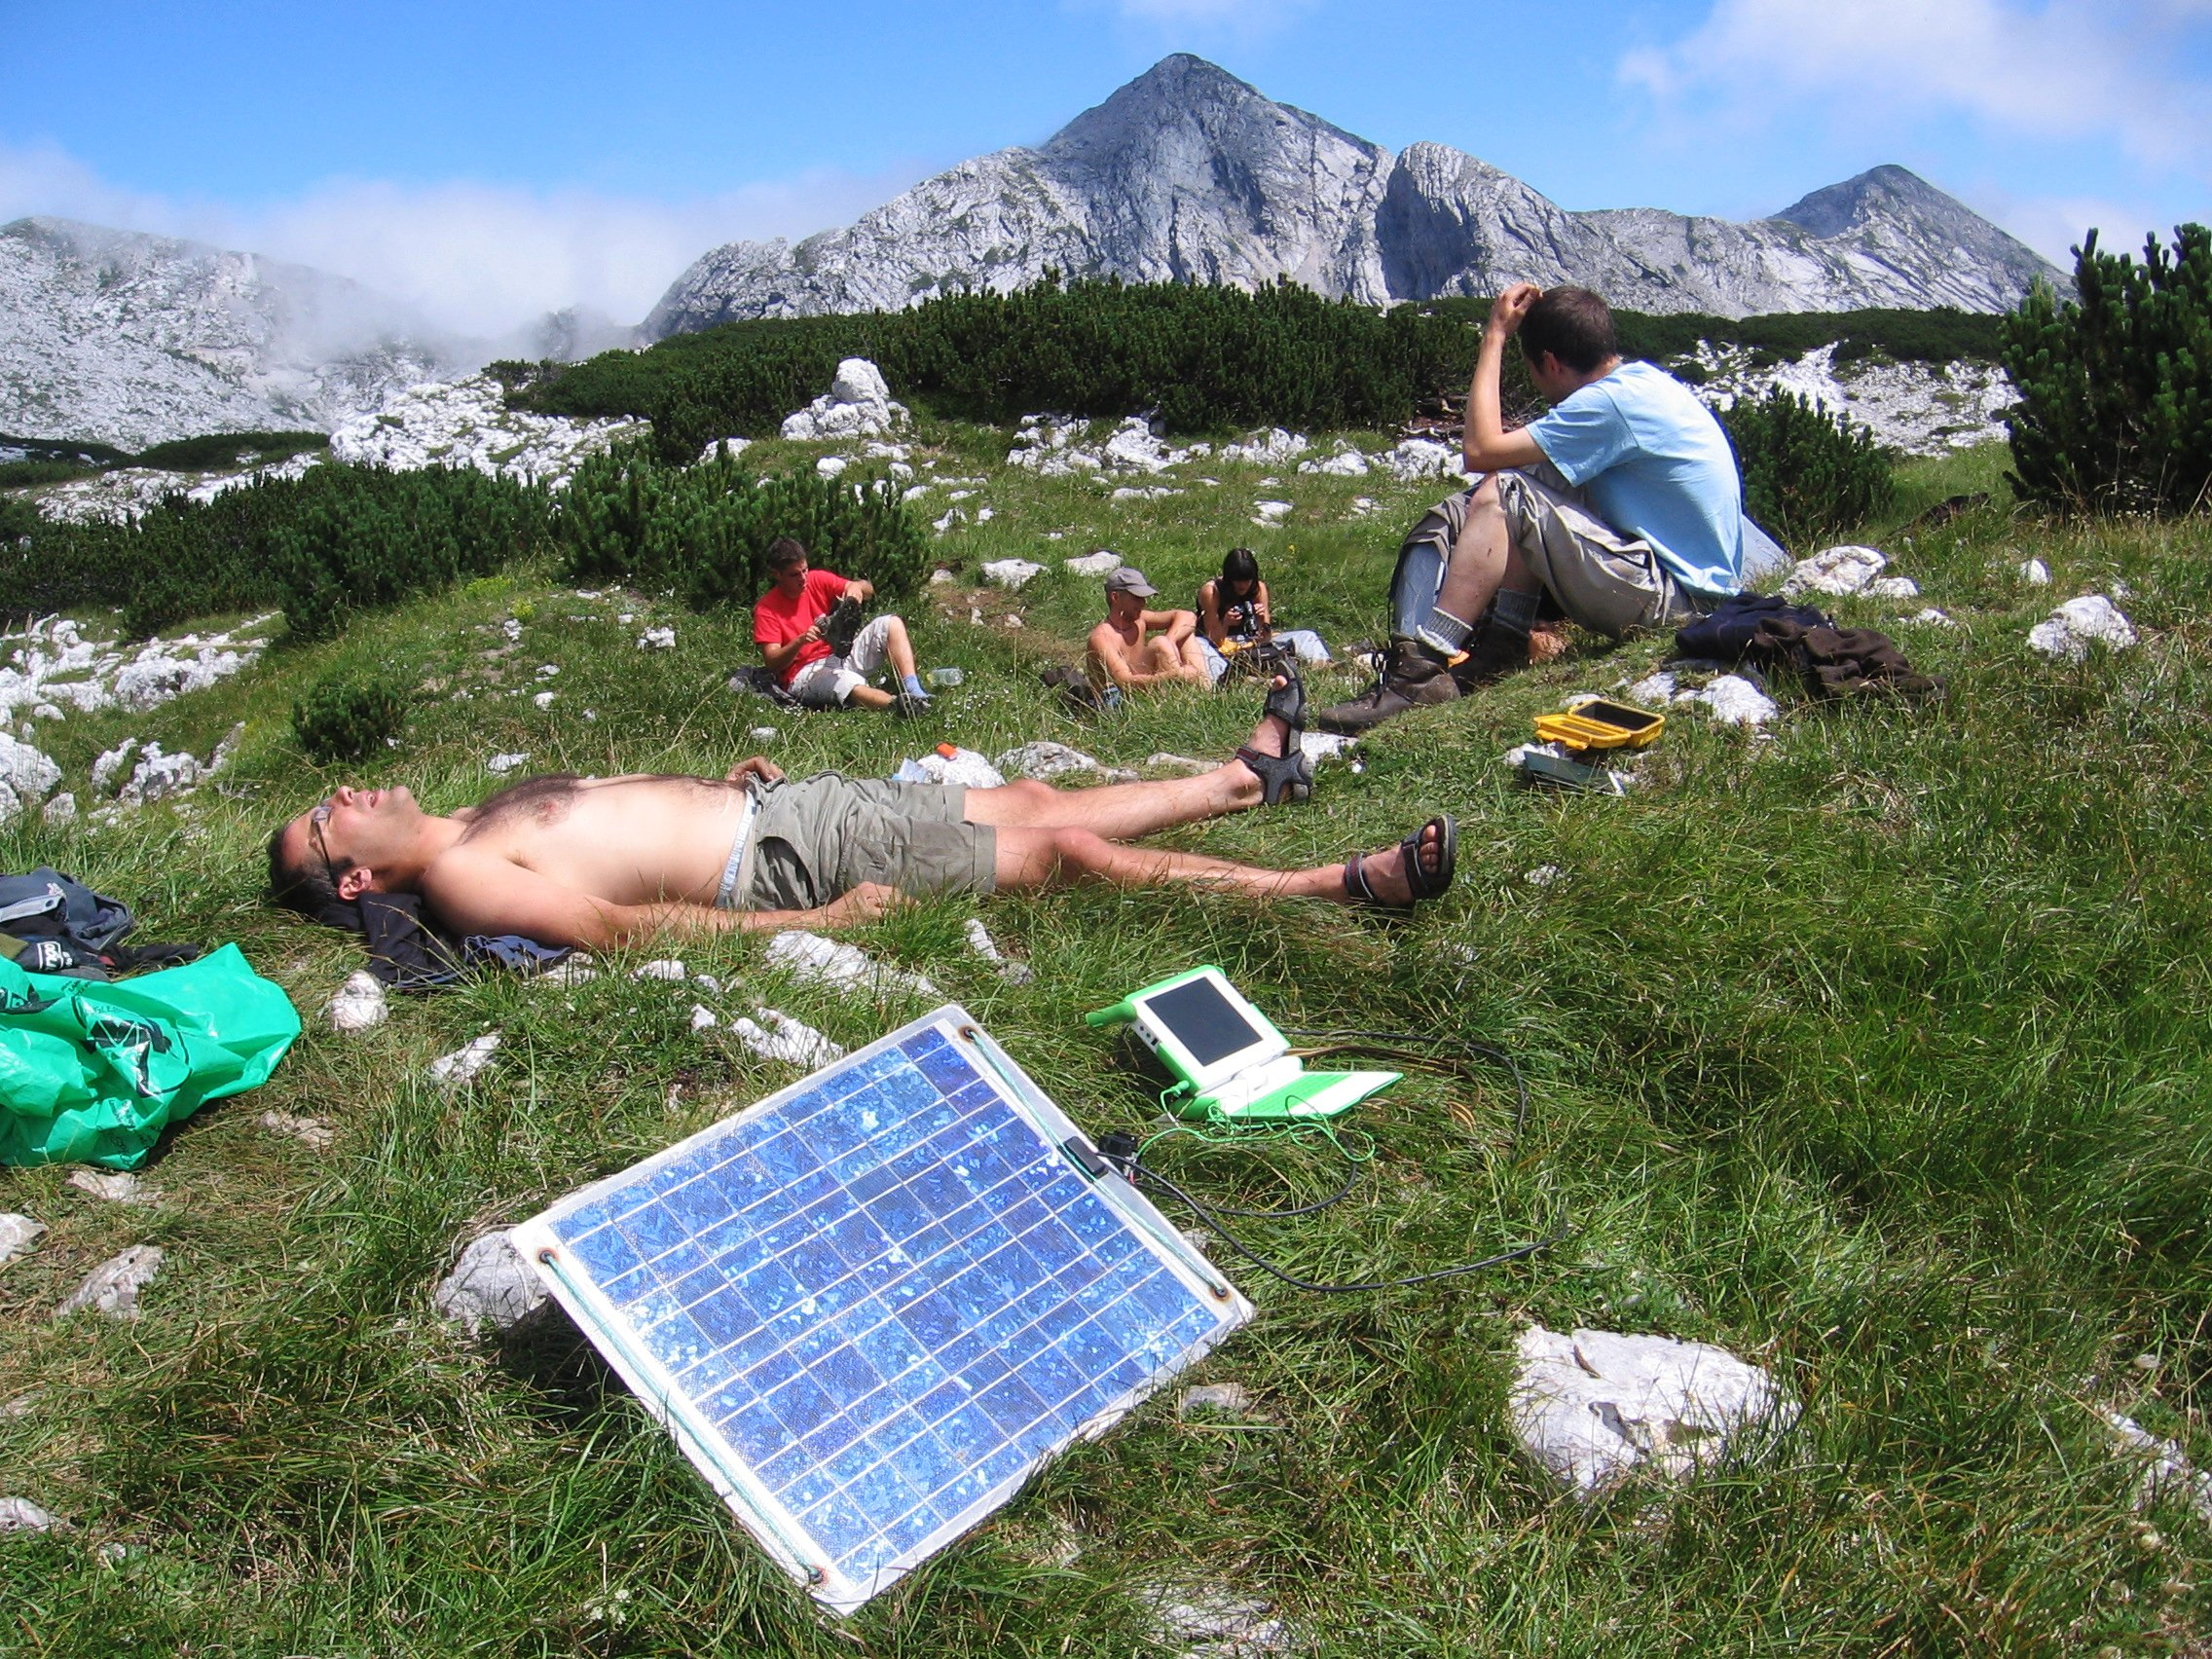
\includegraphics[width=\linewidth]{2008/diary/Jarvist Frost - canon a520 - faff on the plateau with a laptop--orig.jpg}}
\caption{The expedition laptop is one of the most important pieces of equipment to keep charged up. Here, cavers relax on the plateau while the sun provides power. \pic{Jarvist Frost}}
\end{marginfigure}


As such, attention shifted to higher leads to try and secure a
connection in 2008. From the \passage{Something Fishy} chamber a series of
pitches were explored which included the impressive \passage{Dangermouse}. The leads at the bottom are rather dubious, but it makes an
extremely pleasant 72m shaft series (Penfold, Dangermouse, Green
Back, Giblet Breakfast) which has a very valuable commodity on it indeed
- a seemingly faithful stream enters halfway down \passage{Dangermouse} and
collects in a secluded 2 m diameter plunge pool.

The \passage{Captain Kangaroo} series is extraordinarily dry after
\passage{Bonus Chamber} (it is actual dust, not water vapour, that ruins
flash photos in this part of the cave), and the water on
\passage{Dangermouse} is likely to be an important part of future
underground camping plans for 2009.

From \passage{Kill'em All}, a number of avens are noted. One of these was
gained by a rather gung-ho climb with uncertain belay to reach rift that
led away from the pitch. On a future trip, the rigging was improved to
an acceptable level and the rift was pushed to a squeeze. This soon gave
in to hammer attack, and led on to a initially upsetting pitch head.
There was clearly something big and echoing below, but the pitch head
was initially a fair squeeze for an anorexic cat! Disturbingly,
considering it was also our floor, the rock around the pitch head
shattered easily and with a few hours of work produced something
probably passable. The rotten nature of the rock was a concern when
placing the belays, and gained this section of cave the name
\passage{Cheesecake}. A short 10 meter pitch dropped onto an epic rock
bridge in a large chamber, with shafts disappearing down (perhaps
combining below) on either side with multiple second free falls. A
notable rift led off South (towards \passage{M2}) from the far side of the
chamber, but required a bolt traverse out to it. By survey, this rock
bridge is 21 meters directly above \passage{Dark Tranquillity}, so it
is likely that at least one of the pitches connects.


\begin{marginfigure}
\checkoddpage \ifoddpage \forcerectofloat \else \forceversofloat \fi
\centering
 \frame{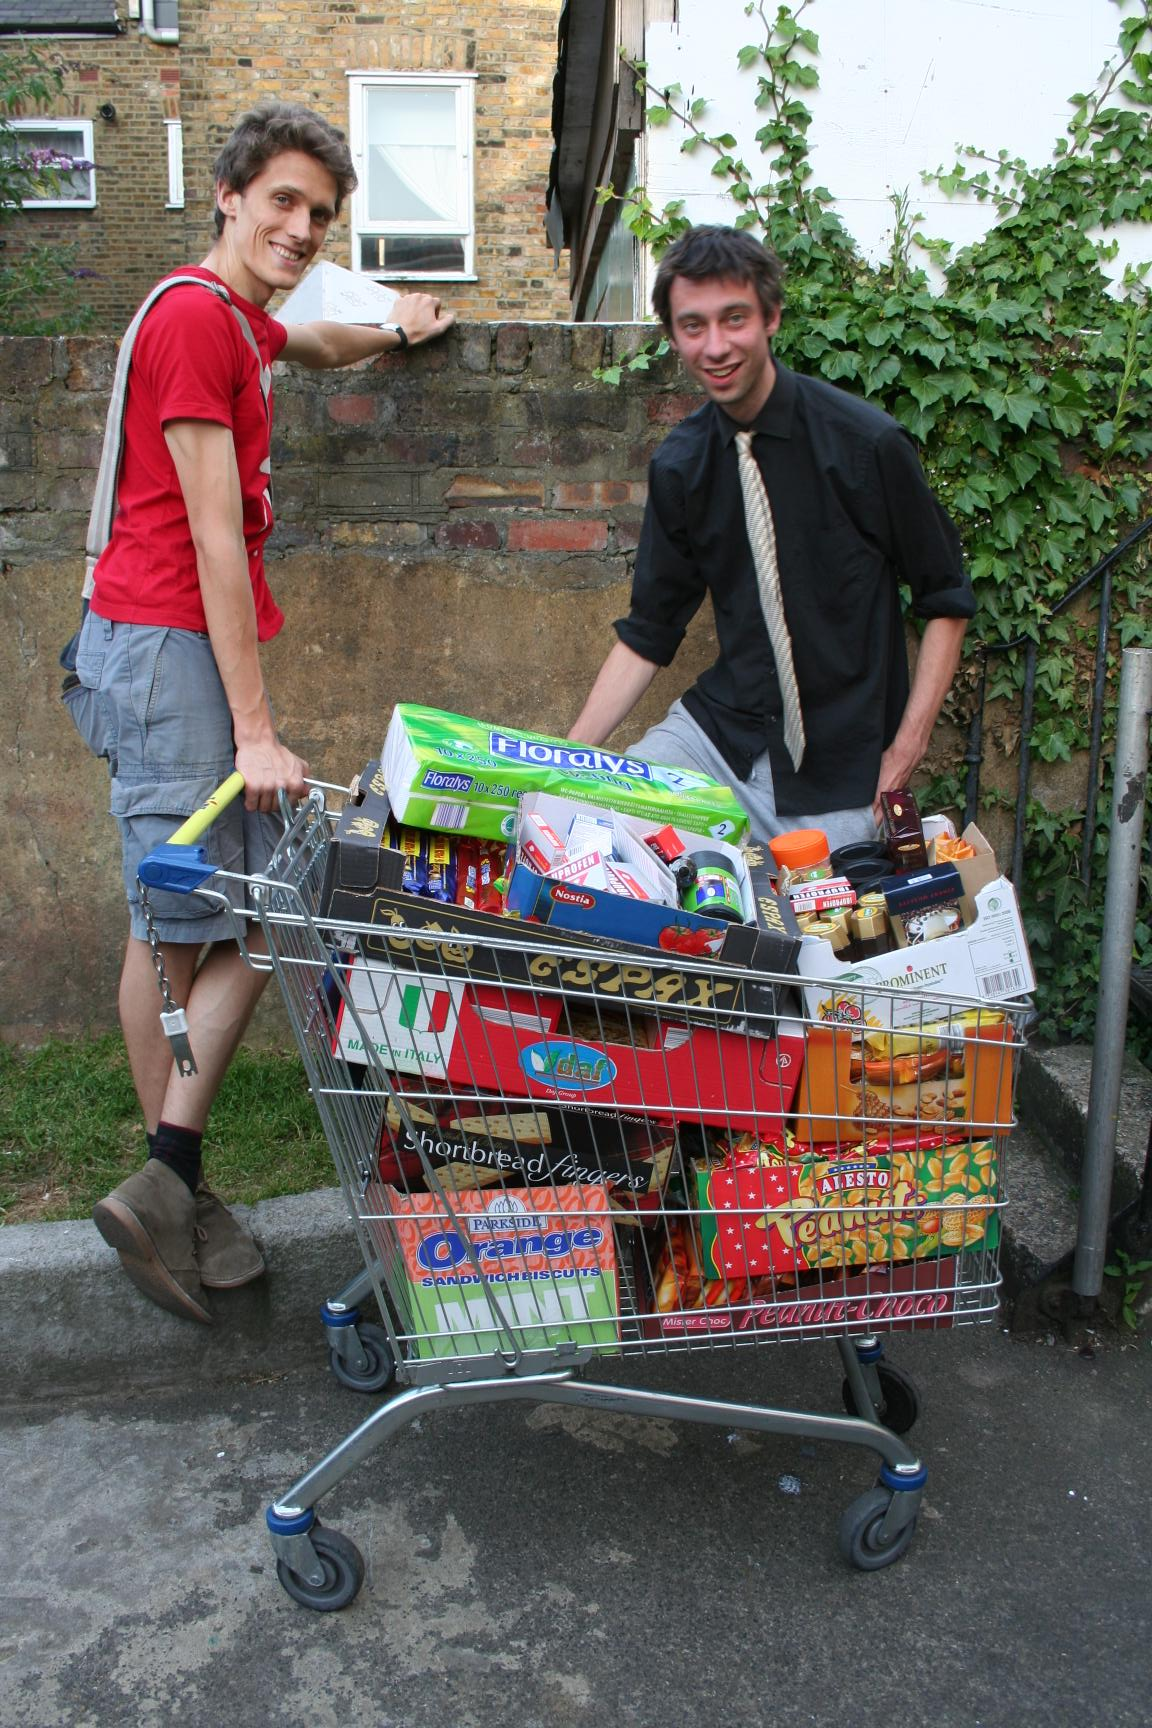
\includegraphics[width=\linewidth]{2008/diary/lidl.jpg}} 
 \caption{Several food purchases are made in the UK during run-up to expedition, sometimes months beforehand - but the final physical shop is never a one-man job. \pic{unknown}}
 \label{lidl food}
\end{marginfigure}



Due to a shortage of gear, a trip was made down the `\passage{Olympic
Rift}' arm of \passage{Captain Kangaroo} to recover equipment and scavenge
rope from the (left rigged since 2007) pitches. The exploration end was
a tight rift leading to a very large space, most likely a re-connection
to the \passage{Space Odyssey} / \passage{Concorde} pitch in the main \passage{Vrtnarija} shaft
series. An unsuccessful attempt was made on the squeeze - it required
expanding. The pitches were derigged and the rope removed to the bone
dry \passage{Traverse Chamber} for immediate use in 2009.

In this region a surface dig started and quickly broke into considerable
passage with a large draft. This was pushed very actively for a number
of trips, before an unfortunate connection being found into \passage{Jelly
Chamber} of \passage{Vrtnarija}. As the explorers at the time commented
``Well, at least its 800 m deep now!''. This \passage{Vilinska Jama} entrance
demonstrates the worth of spending time and effort on surface
excavations, as well as pointing to the plausibility of checking all the
small side passages in established systems.

Above the \passage{Vrtnarija}/\passage{Vilinska} valley is a limestone
pavement that extends from beyond the entrance to \passage{M2}. Here a
surface cave, \passage{E1}, was discovered in 2007 with a $\approx$ 20
m entrance pitch. During 2008 some stones were excavated to an extremely
tight (sub human) sized pitch head blowing strongly. This will require
chemical persuasion to pass, but due to the (now surface surveyed)
location, is a cave of some interest for 2009. Strangely for a surface
cave it has some well defined cave formation (large meander), which
appears to have been saved from infill by an overhanging entrance and
position next to the edge of the plateau.

On the mountain we were joined for a couple of weeks by the younger
generation of the Slovenian JSPDT. The majority of their efforts were
directed to a cave on the Western edge of the plateau, gained by \bignote{a
rather jaw-dropping abseil} of 100 m into the mile-deep \passage{Tolminka} valley!
This cave \passage{Monatip}, whose entranced was noted in 2006 and exploration
begun in summer 2007, is very different in nature to the other mountain
caves, being mostly horizontal with the entrance at 1730 m appearing to
be a dried stream way. Monatip was extended to a total surveyed length
of 710 m, before connecting into the \passage{Primadona} / \passage{U-Bend}
system at -151 m. The exit via the easy \passage{Primadona} shaft system
was welcome!

It is unclear whether \passage{Monatip} will be revisited in the future.
Some of the original enthusiasm for its exploration was it heading
South-East into `blank mountain', but unfortunately it quickly developed
back towards the South-West and \passage{Primadona}. However, it certainly
indicates that \passage{Primadona} itself is a very fertile area for
further exploration.

\tweet{10:39PM Aug 8, 2008}{Mona connected to Primadona,making the western plateau caves ~3.7km long.Carried snow,which has provoked worst storm of expo! Jarv }

Also on the Western Plateau is \passage{Planika Jama}, discovered
simultaneously with \passage{Monatip}. Far more vertical in nature and
partially choked with snow, this was pushed to an ice filled chamber
with `phreatic like' blow holes through the ice. Unfortunately this
original chamber was not reached due to the shifting ice levels - lots
of snow fell in the Winter before the expedition, but also a lot of rain
in the spring. In \passage{Planika} this appeared to have drilled a 1 m
diameter hole through the initial snow plug which gained an icy vadose
development which dropped via a short pitch to a tight blowing rift.
Armed with only hammer and chisels, three cavers spent a full day
smashing this rift to reach a tight squeeze into a further chamber.
Exploration was left at this extremity. On another occasion, a window
noticed near a rebelay ledge was pushed (again necessitating the
expansion of tight rift) to gain a large chamber which actually went
higher than the original entrance to the cave.

In \passage{Sistem Mig}, a return was made to the pitch explored in 2007 named
\passage{Plopzilla} (P105 m). The objectives were to photograph the large
pitch, investigate the extension boulder choke on one side of the pitch,
and to derig the rope to \passage{NCB} for use in future years looking at
other possible shafts coming off this neglected area of the system. The
boulder choke was climbed down through for tens of meters, halting when
reaching a committing climb down through the ever unstable boulders.
Once everyone present had confirmed that ``it goes, but I'm not going
there'' they derigged. Unfortunately the long exposure film photographs
taken with the aid of manually fired flashes on abseiling into the shaft
were badly fogged, probably due to the camera not being so light tight
after its many caving trips! A great pity, as the shaft had a beautiful
fluted triangular-prism cross section.


\begin{marginfigure}
\checkoddpage \ifoddpage \forcerectofloat \else \forceversofloat \fi
\centering
 \frame{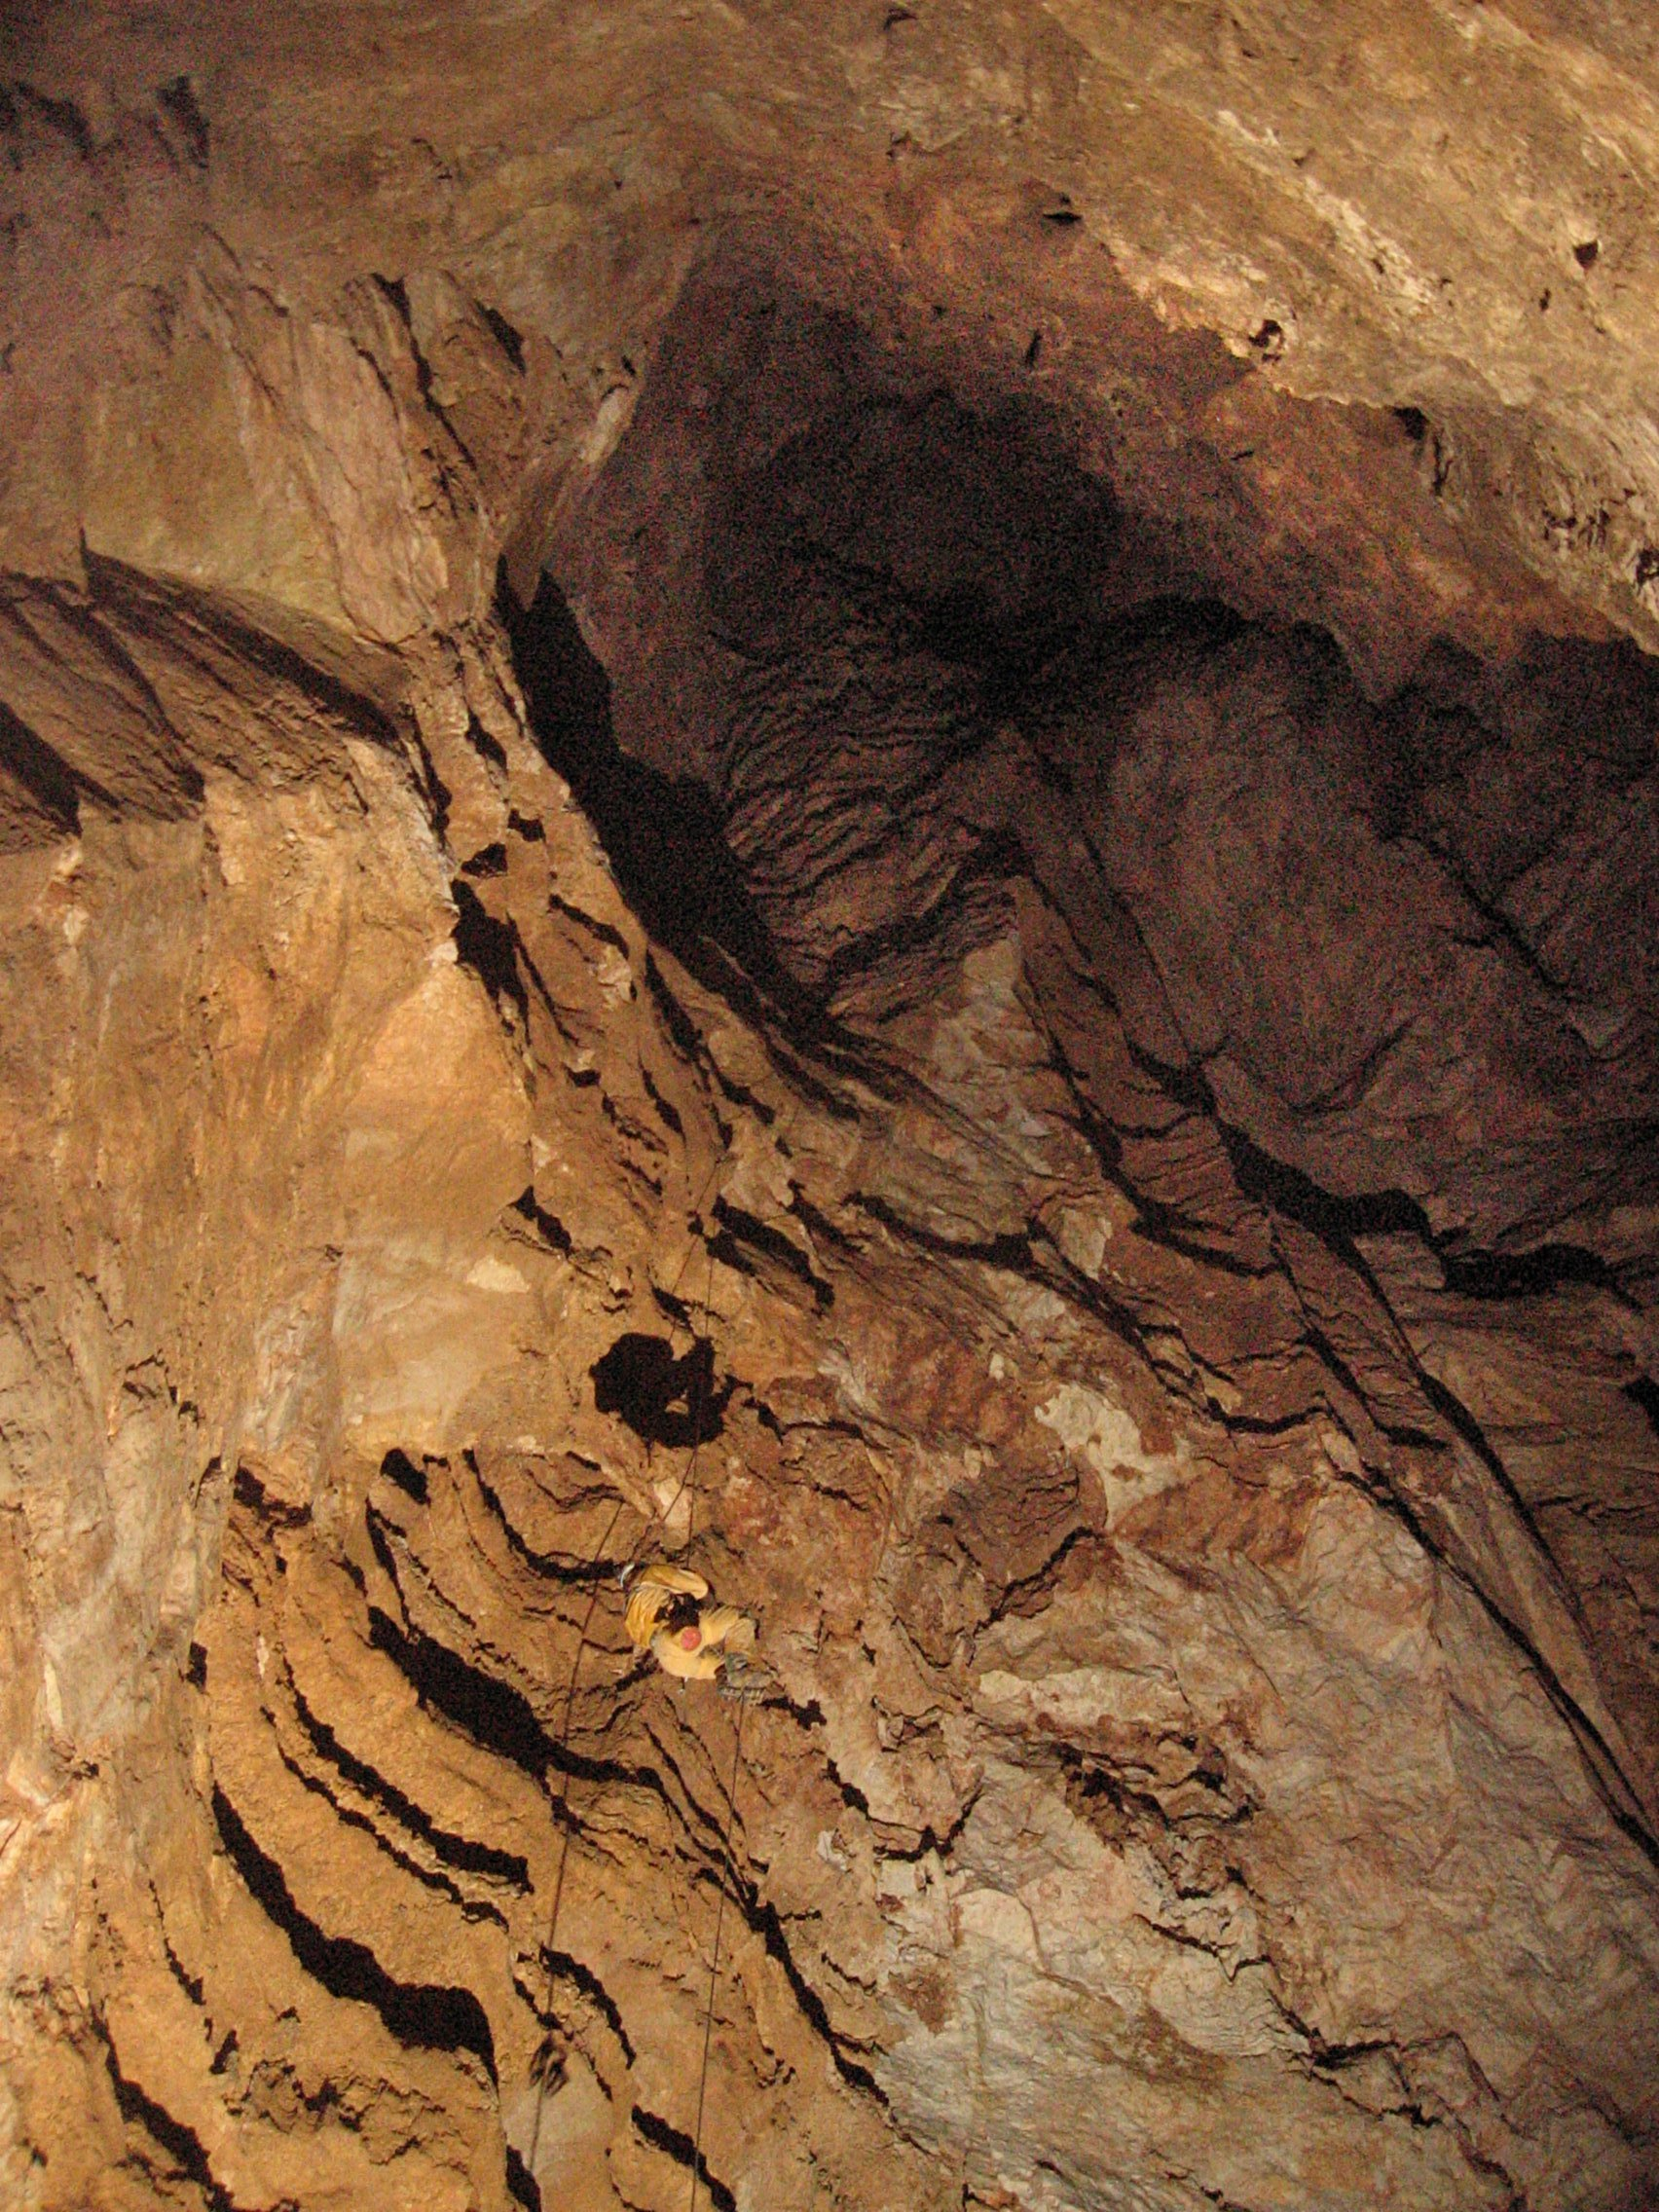
\includegraphics[width=\linewidth]{2008/diary/Jarvist Frost - canon a520 -plopzilla - looking up paul nearly at first rebelay--orig.jpg}} 
 \caption{Paul Hutton ascending \protect\passage{Plopzilla} pitch.  \pic{Jarvist Frost}}
 \label{paul plopzilla}
\end{marginfigure}


\passage{NCB} still holds interest for us, for though it was discovered in 1995
and provided the key for the discoveries of 1996, it has since been
visited rarely (due to its long distance in time from the surface).

A fair amount of surface prospecting has been concerned with investigating
the clear valley located on the mountain top above which contains the
small \passage{M15} and \passage{M17} caves. \passage{M17} was re-entered but found to be choked with
ice. Small caves were found nearby - initial digging has been started.
\section{Across the mountains -- an unexperienced way to reach
Mig}

After two years with the ICCC, I finally made the decision to become a
Migovecer. Having done some cave exploration in Hungary, my idea of such
activities was spending endless hours of underground digging, in
passages of at most a 40 cm high, half-filled with dirty cold
water\ldots{}

\begin{marginfigure}
\checkoddpage \ifoddpage \forcerectofloat \else \forceversofloat \fi
\centering
 \frame{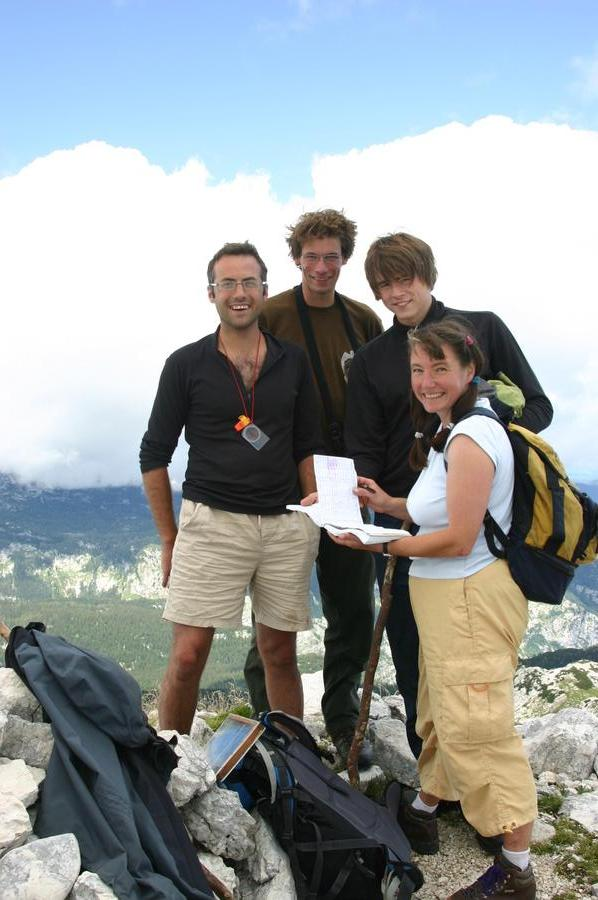
\includegraphics[width=\linewidth]{2008/across_mountains/Gergely Ambrus - DSLR - img_4903--orig.jpg}} 
 \caption{\textit{left to right} James "Tetley" Hooper, Gergely Ambrus, Paul Hutton and Janet Cotter. \pic{Gergely Ambrus}}
 \label{group 2008}
\end{marginfigure}

Numbers better characterise these circumstances than words: in 10 years'
time, my Hungarian club made a steady progress of 400 m, the discovery
of almost every new meter being heavily aided by the products of the
HILTI company. Thus, \bignote{I was eagerly awaiting the \passage[town]{Mecca} of alpine-style
caving} and cave exploration. First, I spent a couple of days at a
Croatian-Hungarian caving expo, which had the double advantage of being
located next to the wonderful \passage[river]{Zrmanja} river, and to the local pub.

But after this wellness-spa holiday, I felt the urge to start true
caving, in the middle of the wilderness, on top of the unknown, mighty
\passage[mountain]{Migovec}. So by hitch-hiking and a train journey, I arrived at \passage{Lake
Bohinj} to meet a friend and toss a day at the lake, after which I had
the illuminating idea of walking across the mountains instead of taking
public transportation to Tolmin and the going up from there.

According to my plans and my speed estimates, the trip could be made in
a day's time if one started early, thus even saving time compared to the
train journey! Thus, early in the morning, I started my ascent up to \passage{Dom
na Komni}. This path does endless hairpins up to the plateau, and no
wonder, I soon realised that the progress was much slower than
anticipated. Inexperienced in the \passage[mountain]{Migovec} conditions, I packed up well:
a complete cooking kit, various layers of clothing, and even some rope
completed the filling of my backpack and a large tackle-sack, which
altogether weighed about 30 kg's, not counting my secret meat stash
weighing a couple of kilos (which became sort of a tradition since
then), so I truly felt like a soldier of the first world war.

By the time I reached the hut, it was clear that the night will be spent
by bivouacking (as the money possibly spent for the hut fees was rather
spent on beer). So I made (or rather struggled) my way to the former
military camp, and set up my sleeping bag in the bushes, my torn poncho
being the only protection against rain - but why would it rain anyway in
such a wonderful, starry night, without a single cloud being visible,
and a wonderful weather forecast for the coming week?

\begin{marginfigure}
\checkoddpage \ifoddpage \forcerectofloat \else \forceversofloat \fi
\centering
 \frame{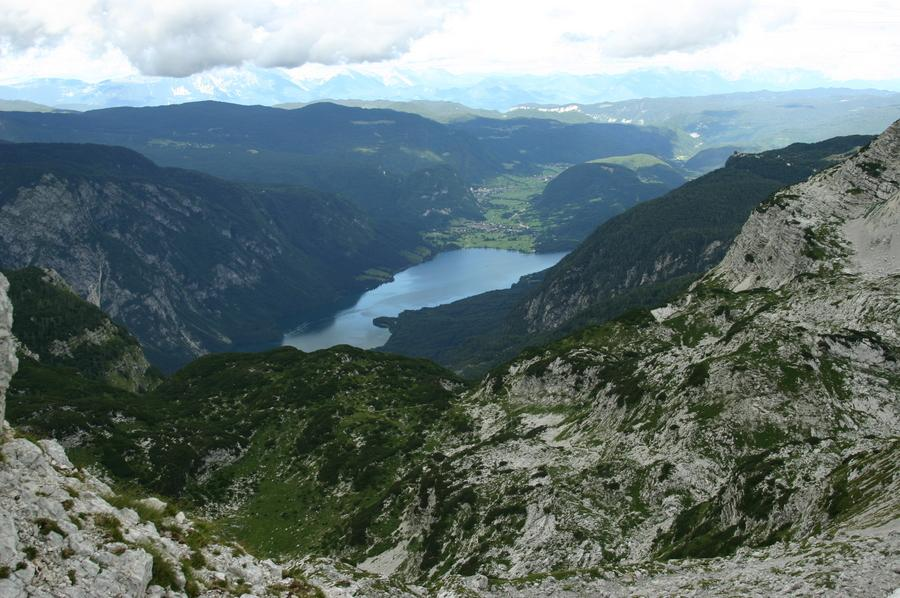
\includegraphics[width=\linewidth]{2008/across_mountains/Gergely Ambrus - DSLR - img_4933--orig.jpg}} 
 \caption{A view of \protect\passage{Lake Bohinj}. \pic{Gergely Ambrus}}
 \label{bohinj gergely}
\end{marginfigure}

Having fallen asleep with such positive thoughts, my dream was
interrupted by a quite uncomfortable noise: thunder! The situation was
not welcoming, and at this moment I was not quite sure anymore whether
it was a good idea to liquidate my accommodation fees\ldots{}

However, a speedy action was needed, and luckily, I discovered a small
black hole next to the bushes. A cave! I imagined my first cave
exploration on \passage[mountain]{Mig} a bit differently, but here it was - speedily, I
managed to remove a couple of rocks blocking the entrance, and enlarged
the hole so that it could fit at least my packs plus half of me, the
other half covered by the torn poncho.

Of course, I hoped for a bit bigger, maybe down to -1000, but for the
moment being, this was sufficient enough to survive the storm - which
job it did at an agreeable level. It was neither dry nor comfortable,
but at least it gave the feeling of some protection against the
thunders, which hit the bushes around me in an alarming frequency.
Finally, the rain stopped, and it was time to recover my possessions,
and to start the remaining part of the journey.

\begin{marginfigure}
\checkoddpage \ifoddpage \forcerectofloat \else \forceversofloat \fi
\centering
 \frame{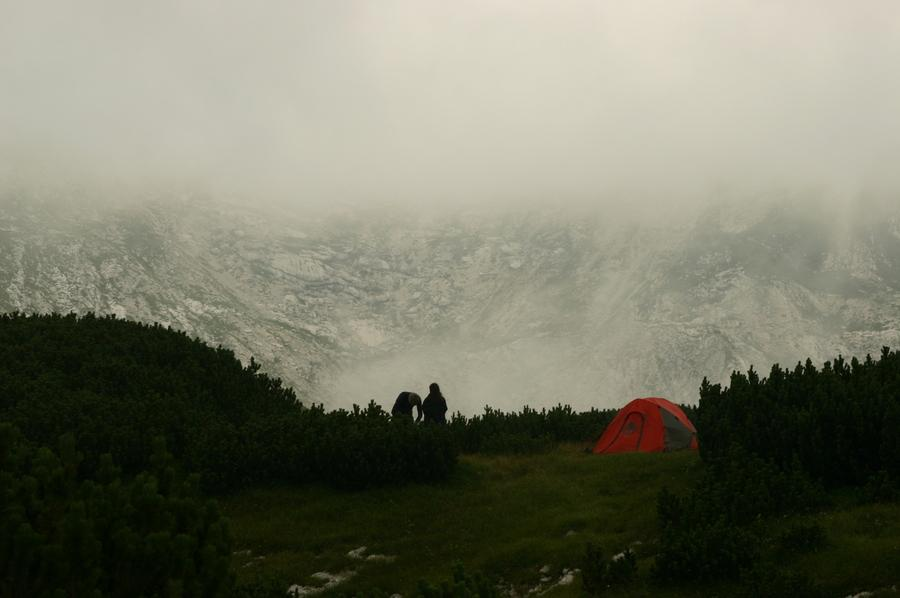
\includegraphics[width=\linewidth]{2008/across_mountains/Gergely Ambrus - DSLR - img_4835--orig.jpg}} 
 \caption{The plateau becomes increasingly difficult to navigate when the cloud comes down, particularly for cavers new to Migovec! \pic{Gergely Ambrus}}
 \label{plateau cloud gergely}
\end{marginfigure}

This was a bit complicated by the mist that now covered everything -
with about 10 m visibility, in the middle of the Northern plateau, with
way too much load, and finally, on the wrong side of \passage[mountain]{Kuk}, it was
definitely not prospecting the most jolly day hike. Somehow I managed to
reach the saddle between \passage[mountain]{Kuk} and \passage[mountain]{Škrbina}, and from here, descended down
to the Migovec plateau following my compass bearings.

The task now was to find the \passage{Bivi}, the only information of which was a
vaguely positioned red dot on my map (I didn't know about the magic
string then\ldots{}) So I wandered a bit up and down, and finally \bignote{at the
edge of total exhaustion, surrounded by fog, a figure appeared on a rock
slab above me} - a person with long hair, a long beard, barefoot and
wearing a long tunic - it could be nobody else, than Jesus! \sidenote{Although Jesus is the longstanding nickname of ICCC member Jan Evetts, on this occasion it was not he.}

At that moment, I realised that I never really imagined Heaven, but if I
did so by any means, the resulting scenery would definitely differ to this
place. I also thought that it would be quite a hard task to collect all
my sins, adding to the final effort of crawling up the slope ahead of
me, by the time I meet Jesus\ldots{} Anyway, I made it to him, and I
gladly realised that the ghostly figure was a most real person: James
Huggett! Thus, my adventurous trip across the mountains has ended, and
soon I was welcomed by the other cavers, and had my first glimpse of the
ever-welcoming \passage{Bivi}.
\name{Gergely Ambrus}

\begin{pagefigure}
\checkoddpage \ifoddpage \forcerectofloat \else \forceversofloat \fi
\centering
\frame{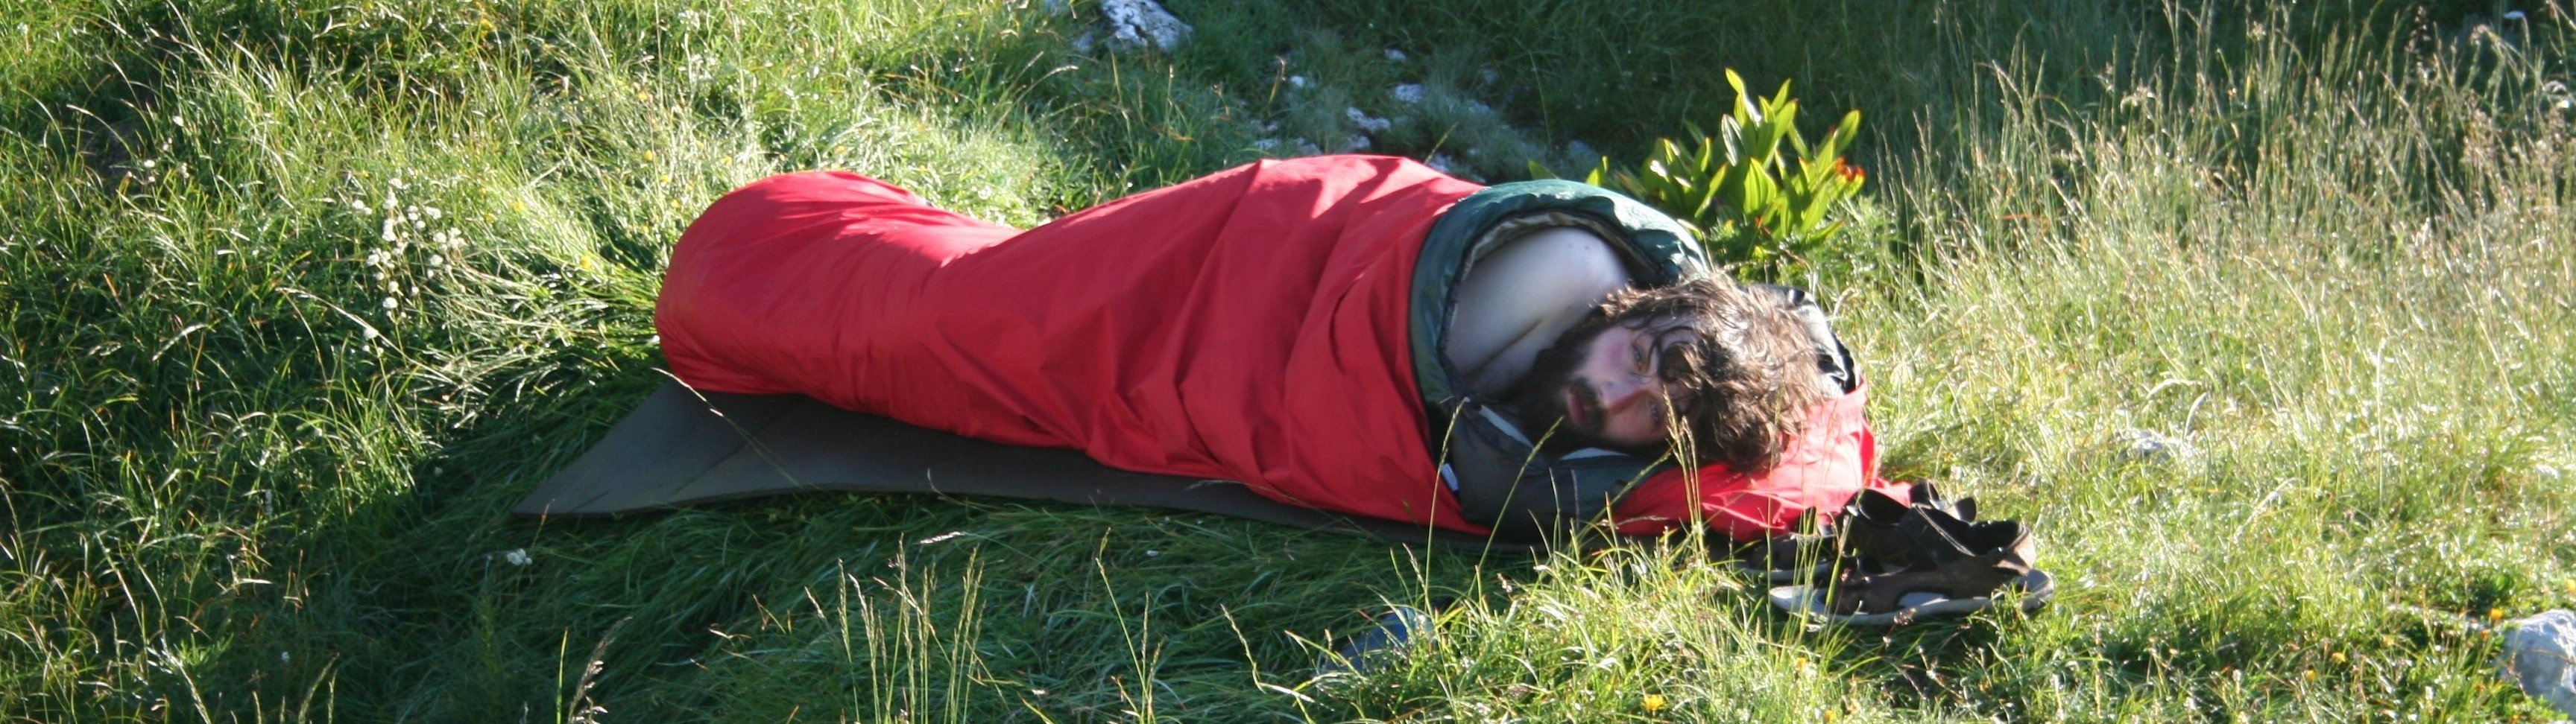
\includegraphics[width=\textwidth]{"2008/across_mountains/Jana Carga - Canon 350D - img_3186 bivi bag on plateau James Huggett--orig.jpg"}}
\caption{James Huggett getting some rest on the plateau. \pic{Jana Čarga}}
\label{Huggett}
\end{pagefigure}
\section{Early trips from the logbook}

\subsection{22.07.08 - Maillons and ladders in \protect\passage{M2}}

 \margininbox{M2}{
     \begin{itemize}
    \item Dan Greenwald
    \item Clewin Griffiths
    \end{itemize}}{\explo}

\begin{marginfigure}
\checkoddpage \ifoddpage \forcerectofloat \else \forceversofloat \fi
\centering
 \frame{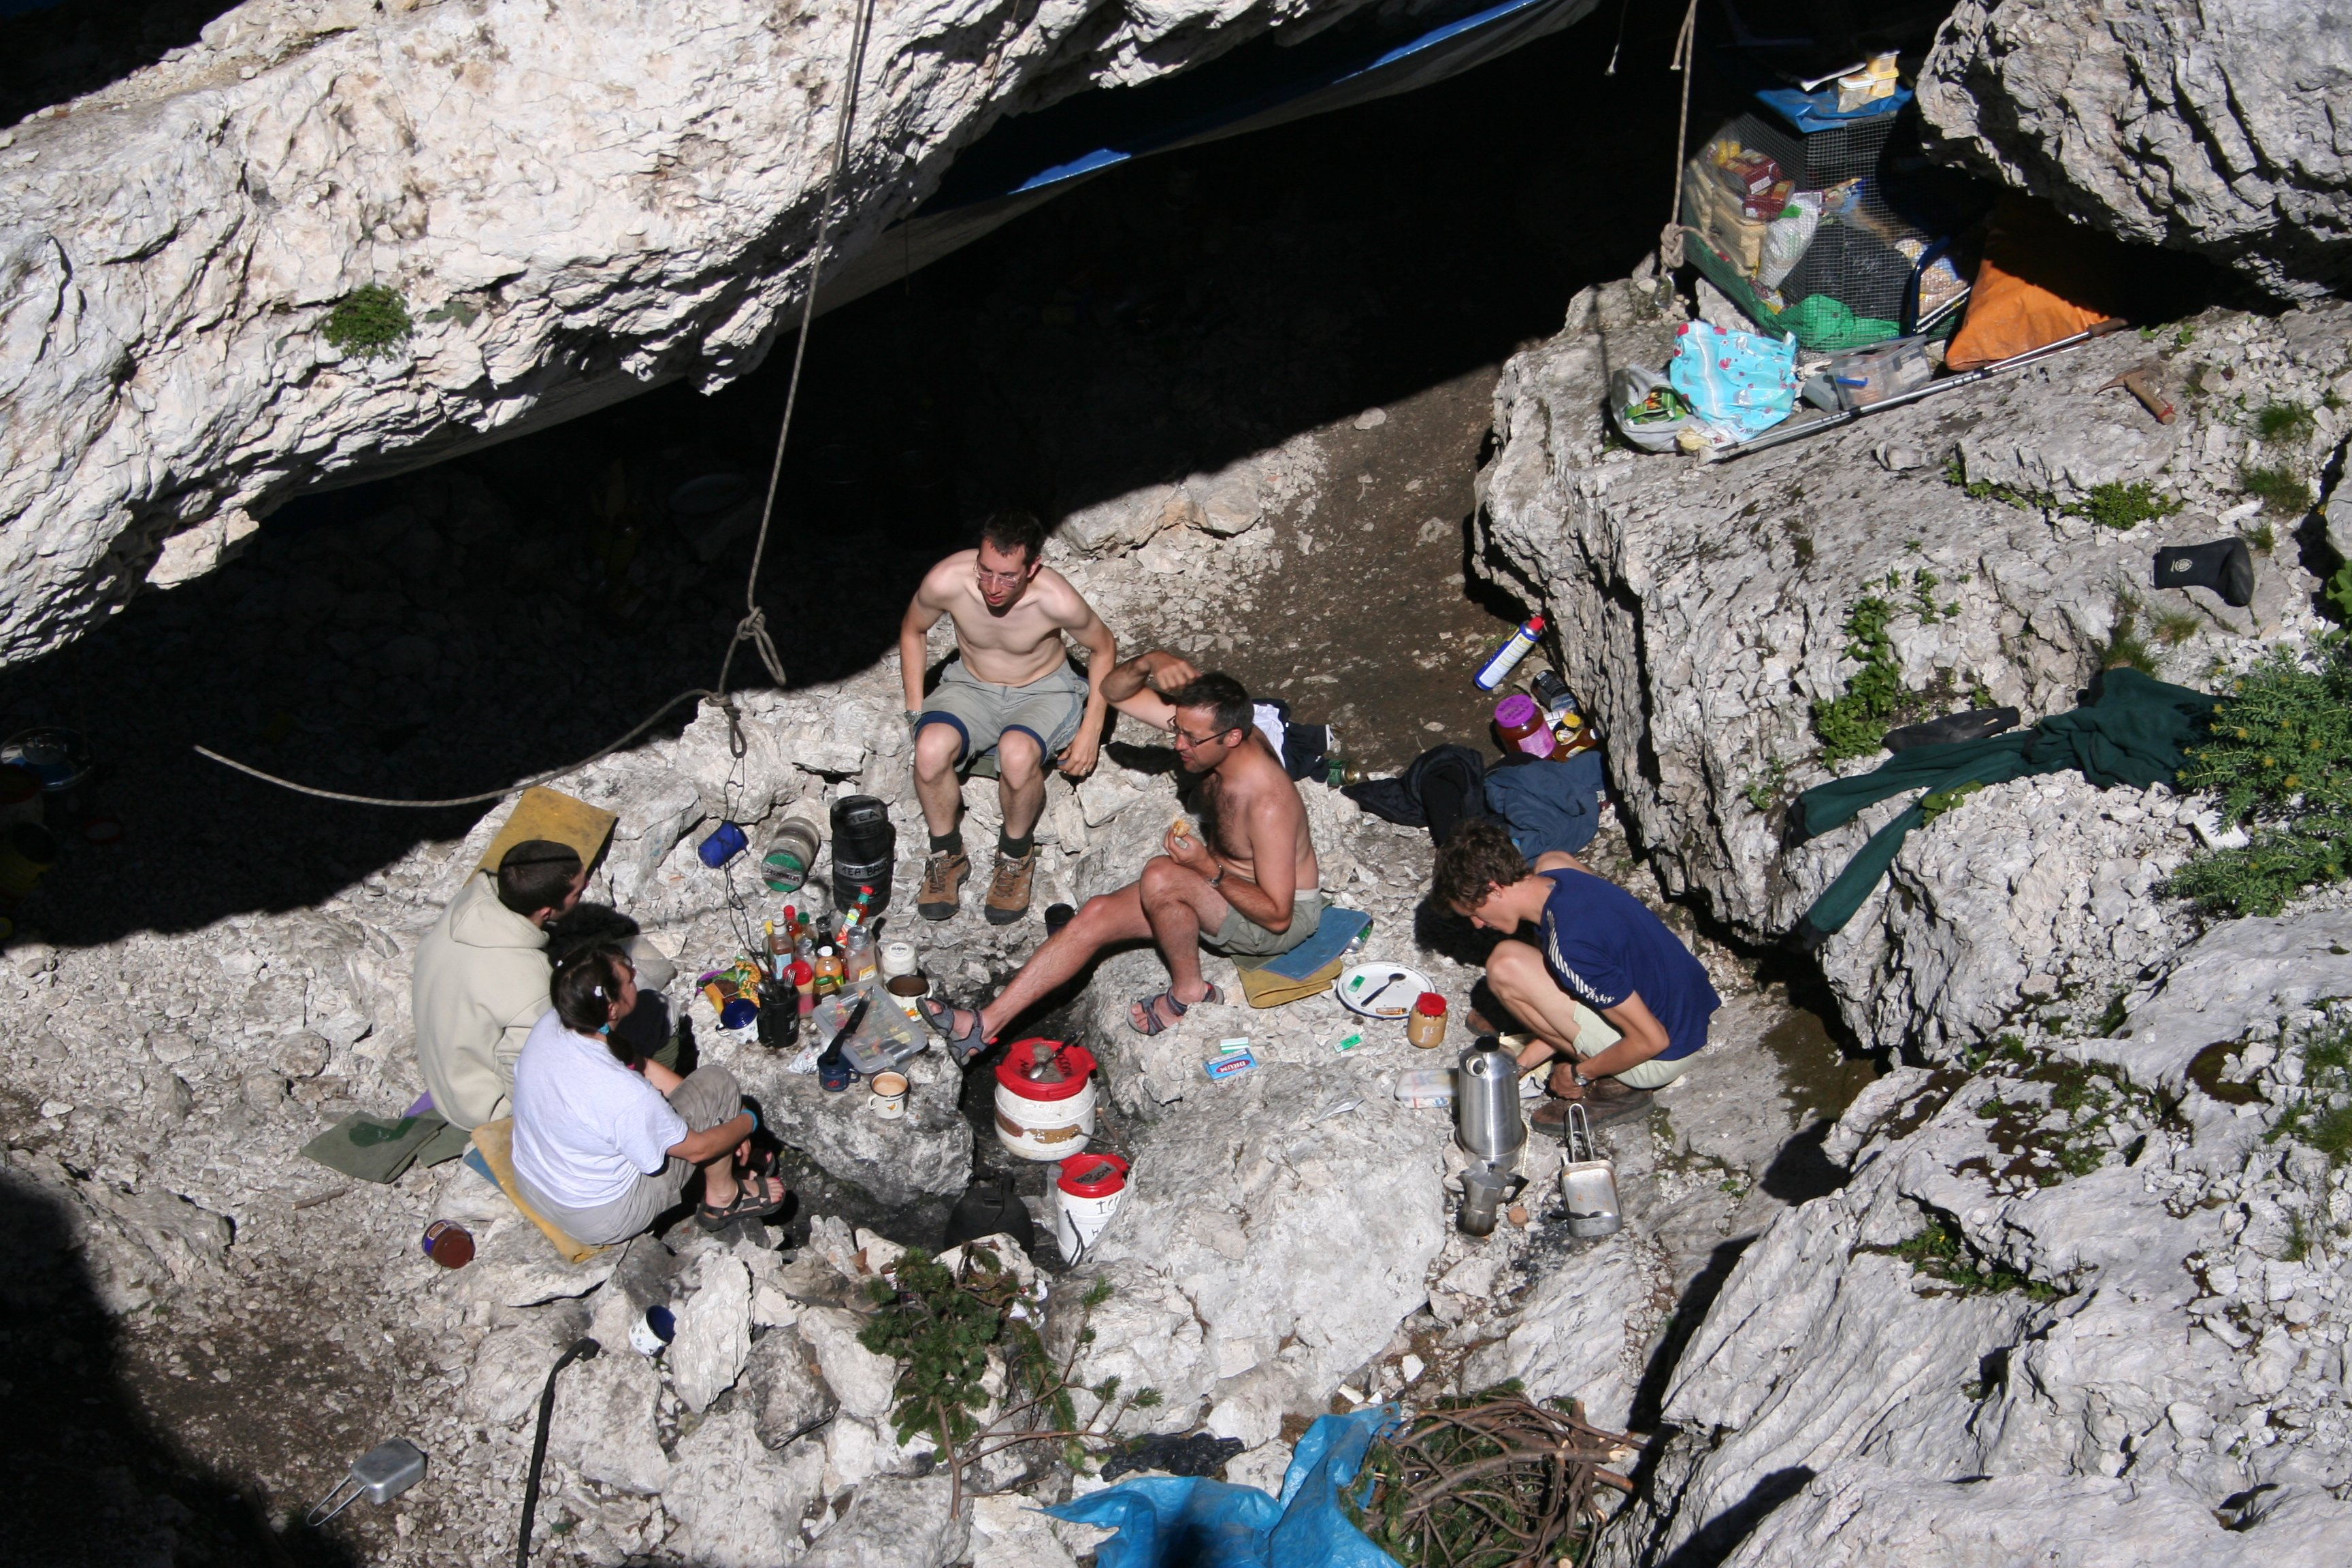
\includegraphics[width=\linewidth]{2008/logbook/Jana Carga - Canon 350D - img_3000 bivi on a sunny late morning--orig.jpg}} 
 \caption{The obligatory morning faff in the bivi takes just as long regardless of weather. \pic{Jana Čarga}}
 \label{sunny morning bivi}
\end{marginfigure}


\bignote{After the obligatory morning faff in the bivvy we started off for
\passage{M2}, then turned back after 20 metres} to get spits and cones.
Wandered over to the entrance which is a stone's throw from \passage{M18}.
The lower entrance drops into a gorgeous daylight shaft with a snow plug
in the bottom and vast amounts of scree.

We then followed the obvious way on, which rapidly gets less and less
obvious, turning into awkward rift. There are a fair few bits of free
climbing before we spotted a piton. Not wanting put all our trust into a
30 year old rusting bit of metal, we put in a couple of dodgy bolts as
back-ups to the piton. It was a straight drop, so we just used a few
metres of rope instead of one of the ladders we had. At the bottom is
ever squeezy and awkward rift ending in a ladder drop (another new
bolt). While doing this, Andy and James appeared, begging for maillons.
We had far too many anyway, so we sent them off happy. At the end of the
ladder drop awaited yet more rift and free climbs. The last climb we
rigged with ladder before taking it off again since it didn't seem to
buy us anything. There it opened out into a reasonable, i.e.~more than 2
m, pitch. We put in two more bolts and then ran into trouble on the
third. Dan bludgeoned the spit teeth into a pulp and we spent about 10
minutes trying ingenious ways to remove the duff spit from the driver.
But we didn't want to do anything which would make it too difficult to
remove if things went wrong. It was already 7:30 pm so we abandoned the
mission.

\name{Clewin Griffiths}

\subsection{22.07.08 - Rerigging \protect\passage{Laurel}}

 \margininbox{Vrtnarija}{
     \begin{itemize}
    \item Andy Jurd
    \item James Kirkpatrick
    \end{itemize}}{\explo}

Set off at 1-ish to rerig \passage{Laurel}. Got to the
top of \passage{Laurel} and found the ropes, but not maillons! Decided to
walk back to bivvy and look for more. Having found none, we left for
\passage{M2} to look for Clew and Dan and their stash of maillons. After a
LONG search for \passage{M2}, we reach \passage{M2} and start going through loose meanders, constantly worried that we were going to shower Dan and Clew in
rock fall. Eventually we get the maillons, walked back to GW, finally
rig \passage{Laurel}. The second rope on \passage{Laurel} is slightly worn and
could do with changing (15-20 m rope needed).

\name{James Kirkpatrick}

\subsection{Captain Kangaroo}

\margininbox{Captain Kangaroo}{
    \begin{itemize}
    \item Jana Čarga
    \item James "Tetley" Hooper
    \item James Huggett
    \end{itemize}}{\explo}

Easy down to \passage{Laurel}. First rebelay under the boulder turned out
to be too tight for our shorter members: add a long sling.

Down to \passage{Pico} no problem, then to \passage{Bonus Chamber},
\passage{Scrotty} would do with some mechanical enlarging. Down to
\passage{Traverse Chamber}. Left 20 m of rope, 5x spit, maillon, hangers,
cones. Rigged a free climb to \passage{Mudslump} (could be improved).

\name{Tetley}

First trip for me down to \passage{Mud Slump}. Lovely trip. It is
actually not that scrotty - at least, not for me\ldots{} :) \passage{Pico}
is an amazing pitch. Will definitely return down there!

\name{Jana Čarga}

   \margininbox{Name translations}{
     \begin{itemize}
    \item Captain Kangaroo – Kapitan Kenguru
    \item Bonus Chamber – Dvorana bonus
    \item Mud Slump – Blatni sifon (Mud sniffles / siphon)
    \item Olympic Rift – Olimpijski meander
    \item Traverse Chamber – Dvorana traverza
    \end{itemize}}{\logbook}

\subsection{\protect\passage{M2} Rigging Part 2}

 \margininbox{M2}{
     \begin{itemize}
    \item Dan Greenwald
    \item Clewin Griffiths
    \end{itemize}}{\explo}
 

Started where we left off --- with 2 ½ bolts placed at
the top of the first real pitch. Dan finished off the last bolt and so
we abseiled down. Using the rope from the pitch I climbed up from the
bottom to see if there was a way on at a high level. There wasn't, but
\bignote{the aven looks promising, although would require a proper climbing trip}.
The bottom of the pitch leads to a 40 m pitch. There was a 70s piton for
backup and a spit at the pitch head. We used the spit (not \textit{too}
rusty) and put a new spit to give a Y-hang. 30 m down was a wide ledge
with garbage from the 70s.

Side track: Off the ledge was a small rift leading to a drop which
we rigged with a ladder. Below that a dodgy free climb lead to a nice
section of wide rift passage with a stream at the bottom and a red
survey dot on the wall. This all closed up completely, so we derigged
the ladder.

At the bottom of the 40 m (\passage{Kletnikov Skropilnik}) a tight rift of black
rock lead to the next pitch. There were no pitch head bolts so we left
this for another trip. 

\name{Clewin Griffiths}

\subsection{25.07.08 - Investigating possibilities in E1\ldots{}}

 \margininbox{E1}{
     \begin{itemize}
    \item Jana Čarga
    \item Jarvist Frost
    \end{itemize}}{\explo}

\begin{marginfigure}
\checkoddpage \ifoddpage \forcerectofloat \else \forceversofloat \fi
\centering
 \frame{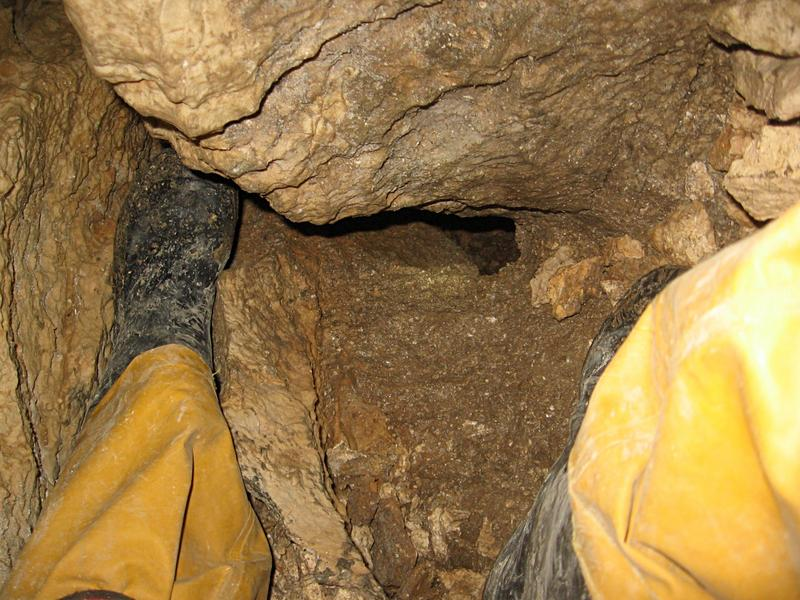
\includegraphics[width=\linewidth]{2008/logbook/Jarvist Frost - canon a520 - e1 - new pitch head.jpg}} 
 \caption{The new pitch head in E1. \pic{Jarvist Frost}}
 \label{pitch head e1}
\end{marginfigure}

Jana pushed the small crawl, which was draughting; went for a while.

We then moved attention to the deep deep crawl, abandoned last year as
dead. It wasn't. But perhaps it should have been. We moved the most
dangerous boulder loitering over the edge and set to work.

Dig dig dig\ldots{}

6 m long, $\approx$ 60° scree slope, terminating in pitch (6-8 m,
as judged by rattling stones).

First few armfuls of rock were stacked, until we started chucking scree
over the edge, boom boom boom. Tidied back to bedrock - too tight -
damn! Strange pitch head, almost T-shaped: water slopping over the edge,
but also a notch cut down ($\approx$ 10 cm wide).

We surface surveyed and tied the centreline to \passage{M2} entrance.
The end of the cave is 40 m above the end of \passage{Goodybag}, \passage{M16}.

We will need a better name before it gets too big → `Mountain Goat
Cave'? Sounds good in Slovene, says Jana.

\name{Jarvist Frost}


\subsection{26.07.08 - 3rd rig of \protect\passage{M2}}

 \margininbox{M2}{
     \begin{itemize}
    \item Andrej Fratnik
    \item James Kirkpatrick
    \end{itemize}}{\explo}

Continued where we left: Andrej rigged \passage{M2}: safely 1st rebelay on
a giant (minibus sized) boulder of dubious stability. 2hrs + 5 rebelays
later we were 20 m from the bottom and out of spits. Damn! Return with 5+
bolts and finish the job some other day. Had a hell of a time getting
out of the entrance rift\ldots{}

\name{James Kirkpatrick}









\subsection{26.07.08 - \passage{M16} $\rightarrow$ \passage{Plopzilla} $\rightarrow$ end of \passage{NCB} (\passage{Zebra} passage)}

 \margininbox{M16}{
     \begin{itemize}
    \item Jana Čarga
    \item Andy Jurd
    \end{itemize}}{\explo}

10 hour trip. 
Re-rigged the way down to \passage{Gladiators'}. 

Also re-rigged a small traverse just after \passage{Club Mig}.

Jana had an epic piss on the ledge in the middle of \passage{Gladiators' Traverse.} 

\margininbox{For Evans' Sake, 2009}{
     "Jana Čarga for her mid Gladiator's traverse relieving of bladder pressure, perched above twin 60m pitches on a wedged rock, with one leg through a harness loop for 'safety'."}{\award}

We check out \passage{Plopzilla}, but have not taken the rope out.

Checked the end of \passage{NCB}. In \passage{Zebra}, 2 ways on:

\begin{enumerate}
    \item 
    A small climb down ($\approx$ 6 m) need to be smashed, remove boulders
    \item 
    Small, tight crawl continuing up \passage{Zebra}
\end{enumerate}

Have taken the Gladiator's old rope out. Amazing trip!
    
\name{Jana Čarga}




\begin{figure*}[b]
\checkoddpage \ifoddpage \forcerectofloat \else \forceversofloat \fi
\centering
    \begin{subfigure}[b]{0.49\textwidth}
        \centering
        \frame{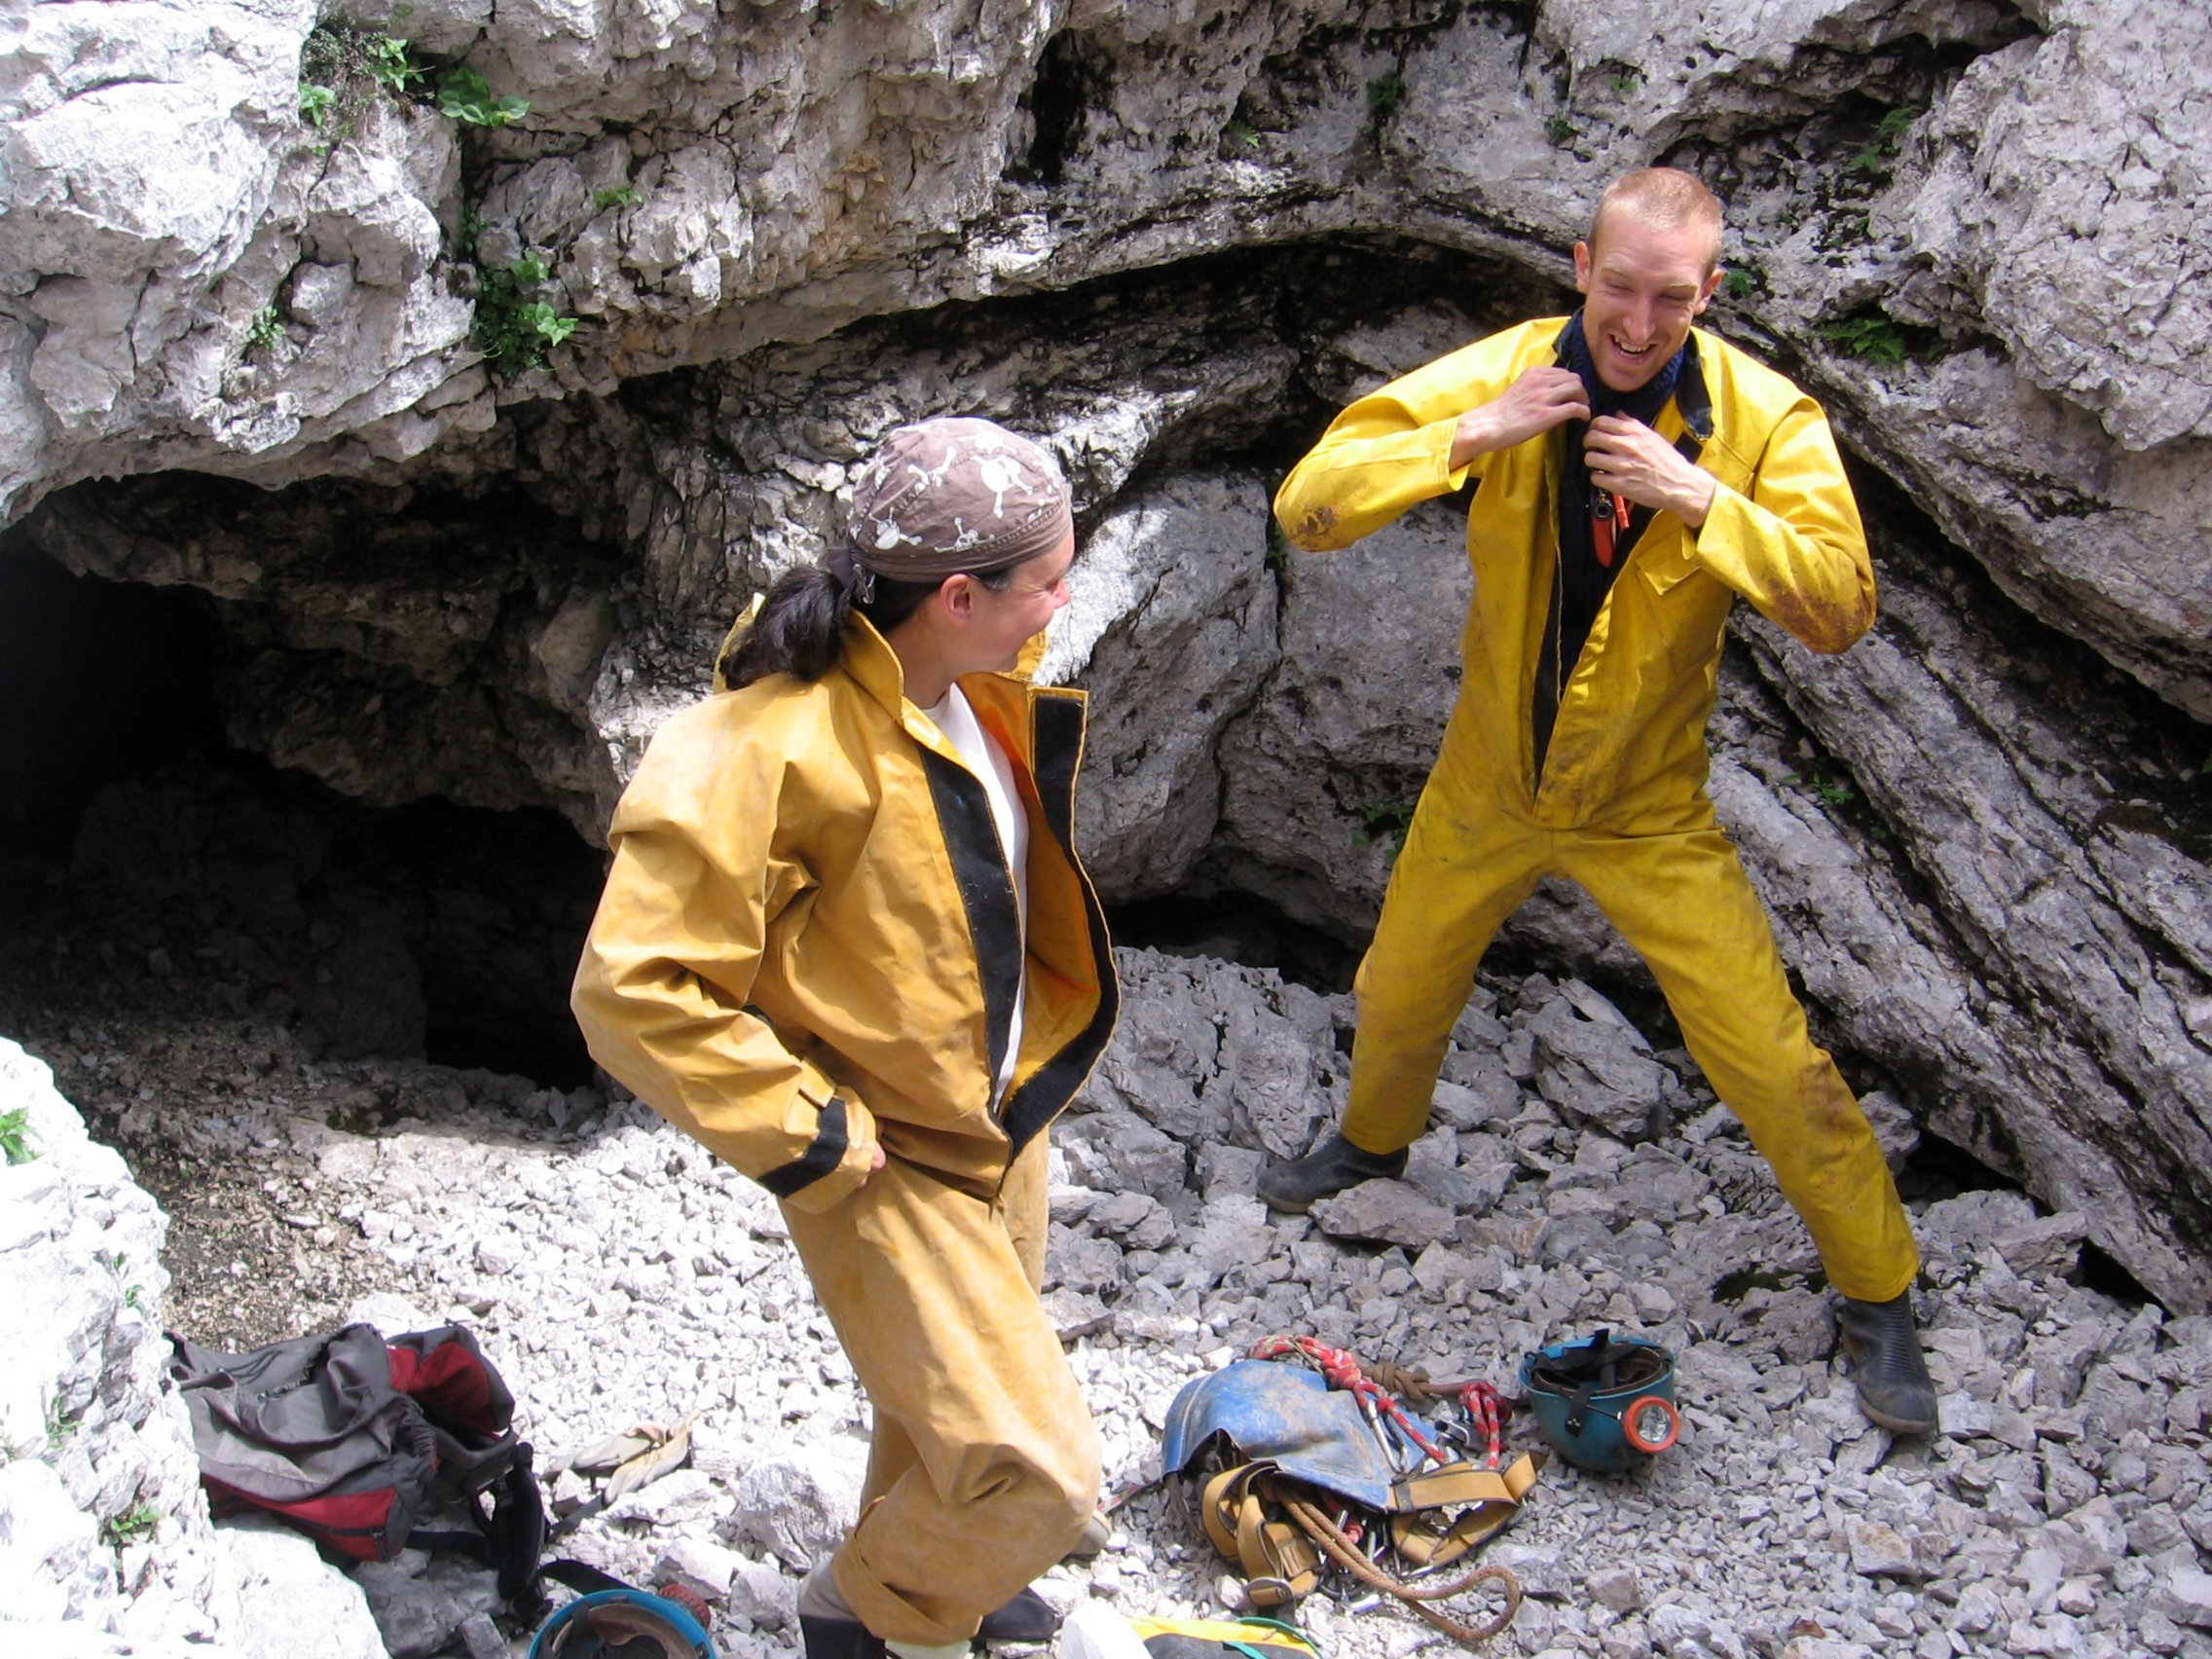
\includegraphics[width=\linewidth]{2008/logbook/Jarvist Frost - canon a520 - sysmig - JC AJ trip - getting ready--orig.jpg}} 
        \caption{Andy and Jana kitting up for the trip outside \passage{M16} \pic {Jarvist Frost}} \label{M16 prep}
    \end{subfigure}
        \hfill
\begin{subfigure}{0.49\textwidth}
\centering
\frame{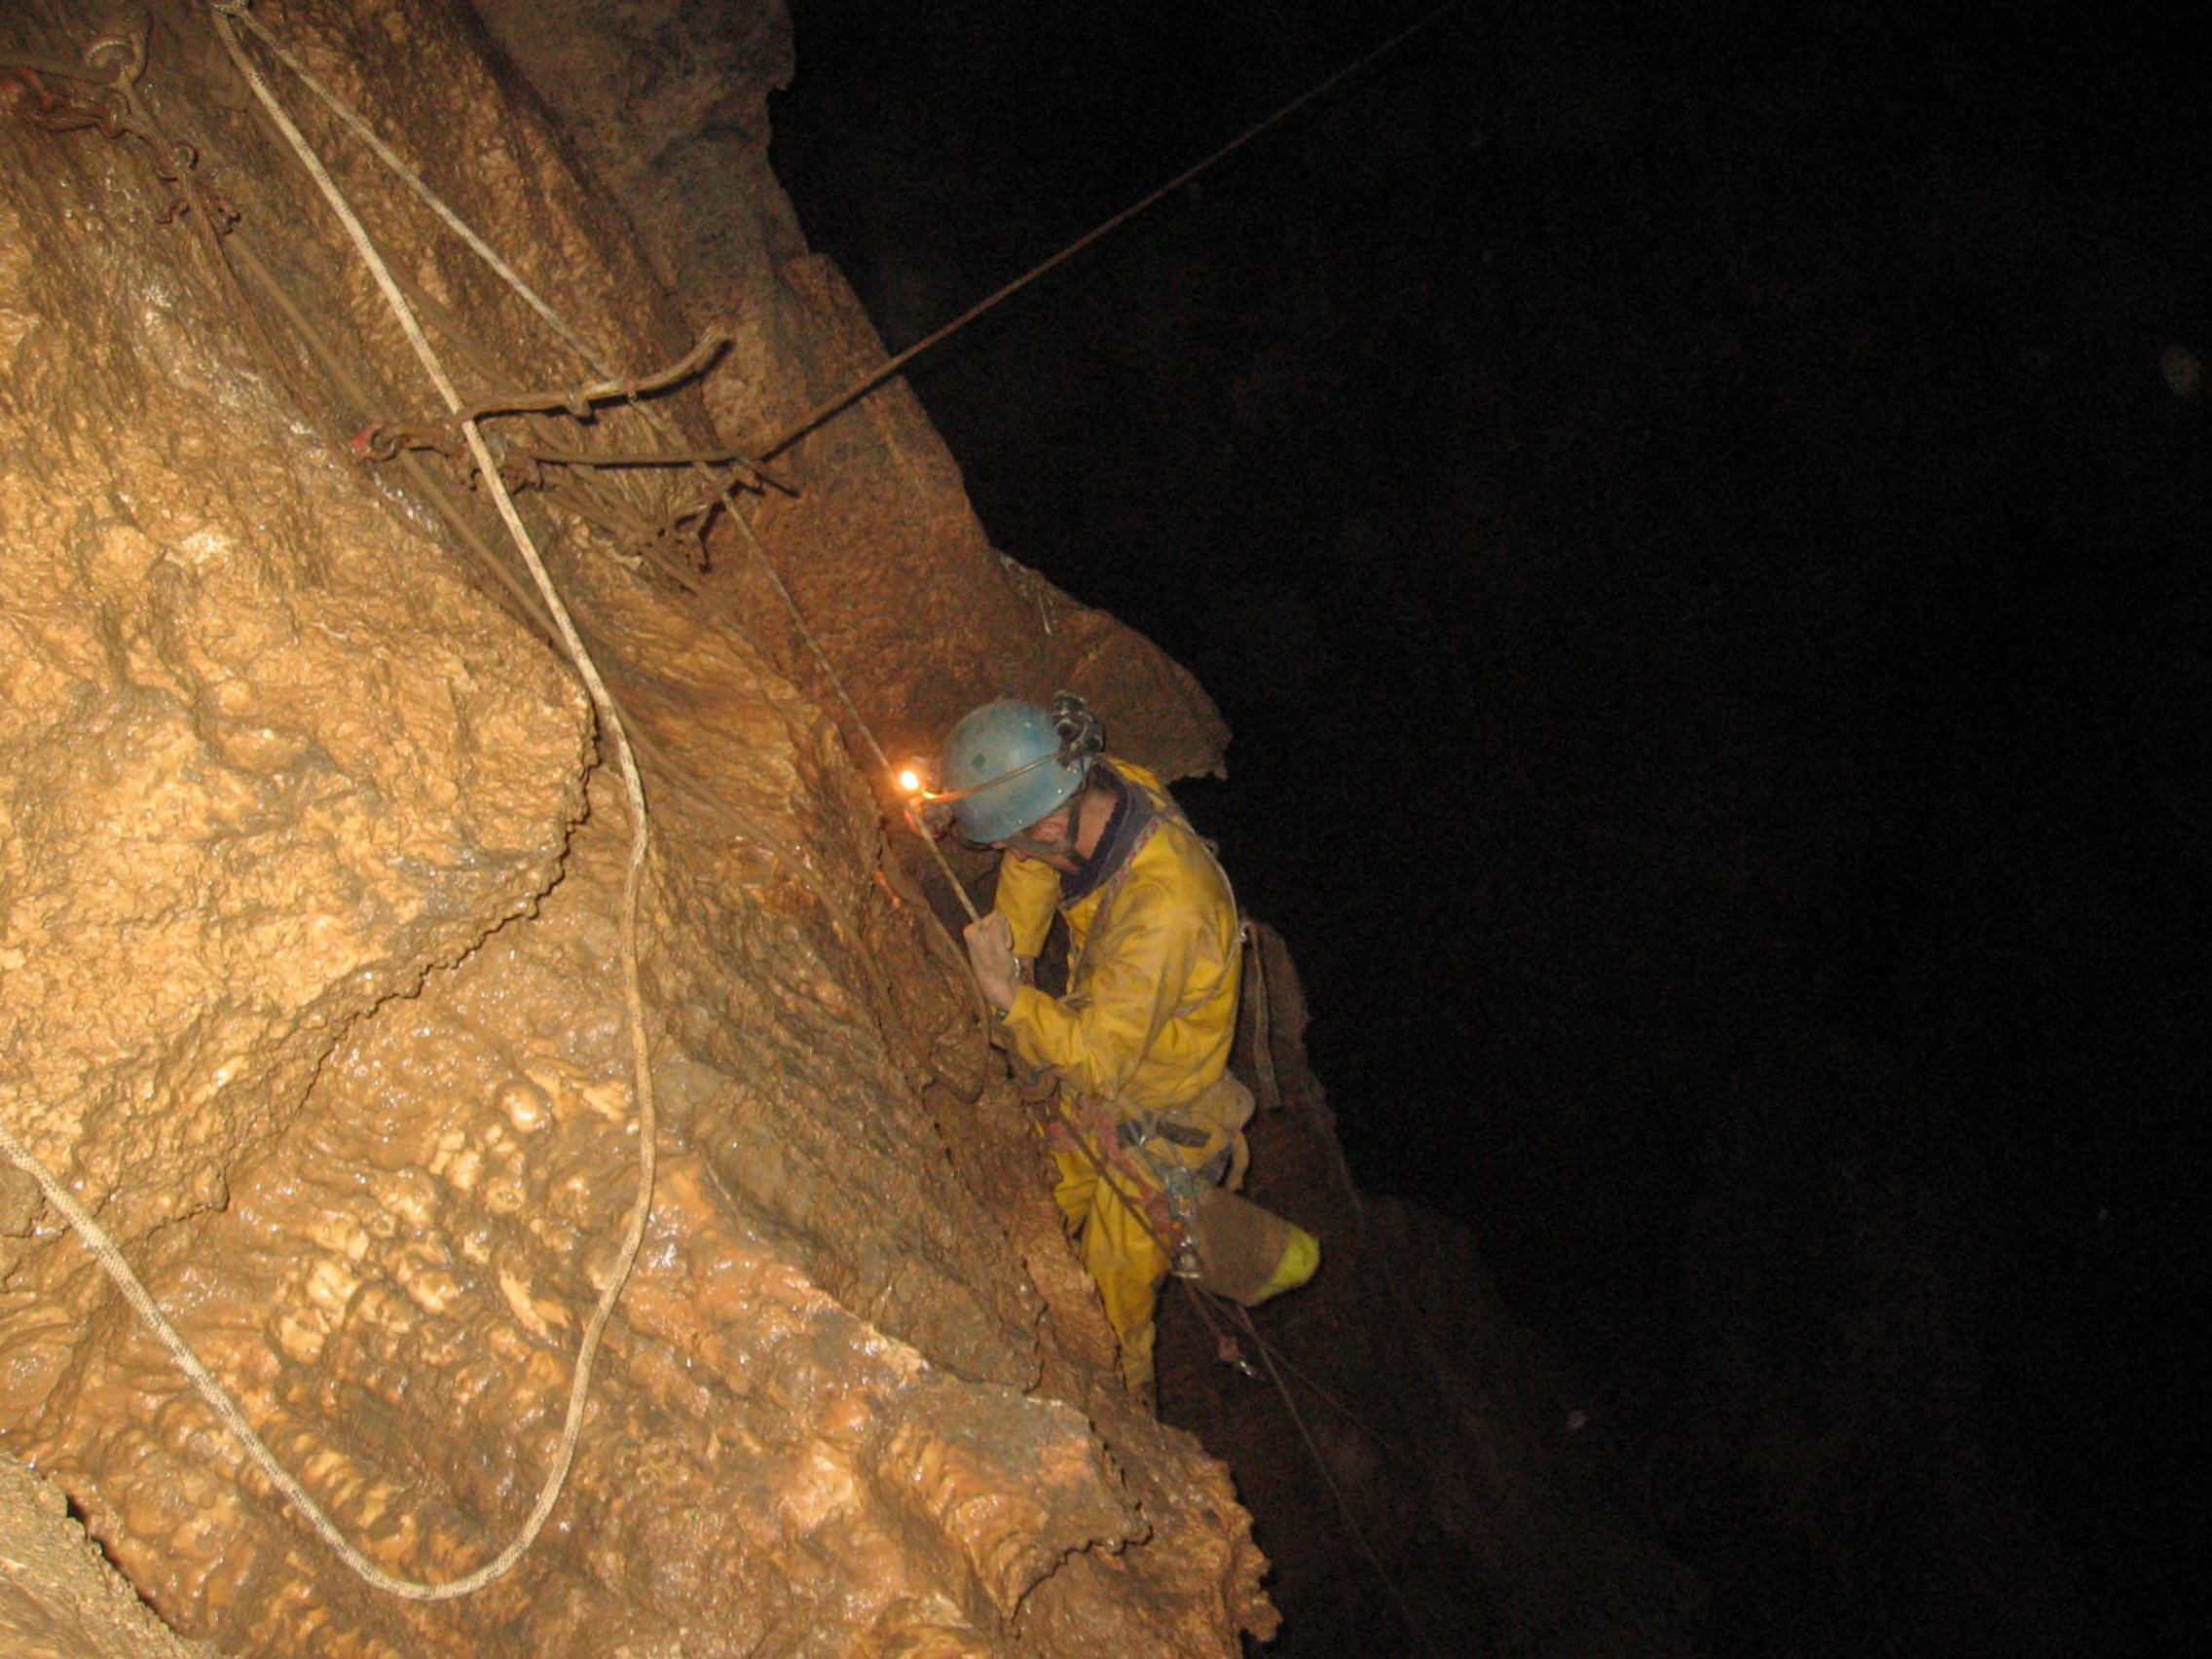
\includegraphics[width=\linewidth]{2008/logbook/Jarvist Frost - canon a520 - sysmig - JC AJ trip - Andy on gladiators--orig.jpg}}
 \caption{Andy negotiating the \passage{Gladiator's traverse} \pic {Jana Čarga}}\label{gladiators}
\end{subfigure}
  \caption{}
\end{figure*}



\section{\texorpdfstring{26/7 Jarv \& Clew →
\emph{Planika}}{26/7 Jarv \& Clew → Planika}}

Ill fated trip! The rerig slowed us down. Clew placed a Y-hang bolt -
went a bit deep, no matter - ``I have a cunning plan''. Wedging a spare
cone lightly into the spit, he protected the thread while cleaning
around. Of course, it didn't come out again. Then he hit a super tight
Alpine-butterfly just 1 m shy of the rebelay. 20 mins of effort, to
prussic up \& have Jarv knaw it open. Then he lost his knife in a
crevass \& spent 20 thoroughly cold minutes digging it out, while Jarv
placed the backup bolt (nice white soft rock). Expanded the chest
squeeze \& finally reached the pushing front rather late. Clew expanded
the pre-pitch squeeze while Jarv rerigged \& then attempted the higher,
better rift.

Rift: Phreatic top slightly less than body crawl sized tube, less than
chest width vadose. But transition zone is very friable. I got
\textasciitilde3 m in, to see 2 m rift → chamber. Drafting \emph{IN}.
Chamber has fist sized boulders in it. Turns right.

GOING!!! ( with instrument of destruction) Jarv

\begin{figure*}[t]
\checkoddpage \ifoddpage \forcerectofloat \else \forceversofloat \fi
\frame{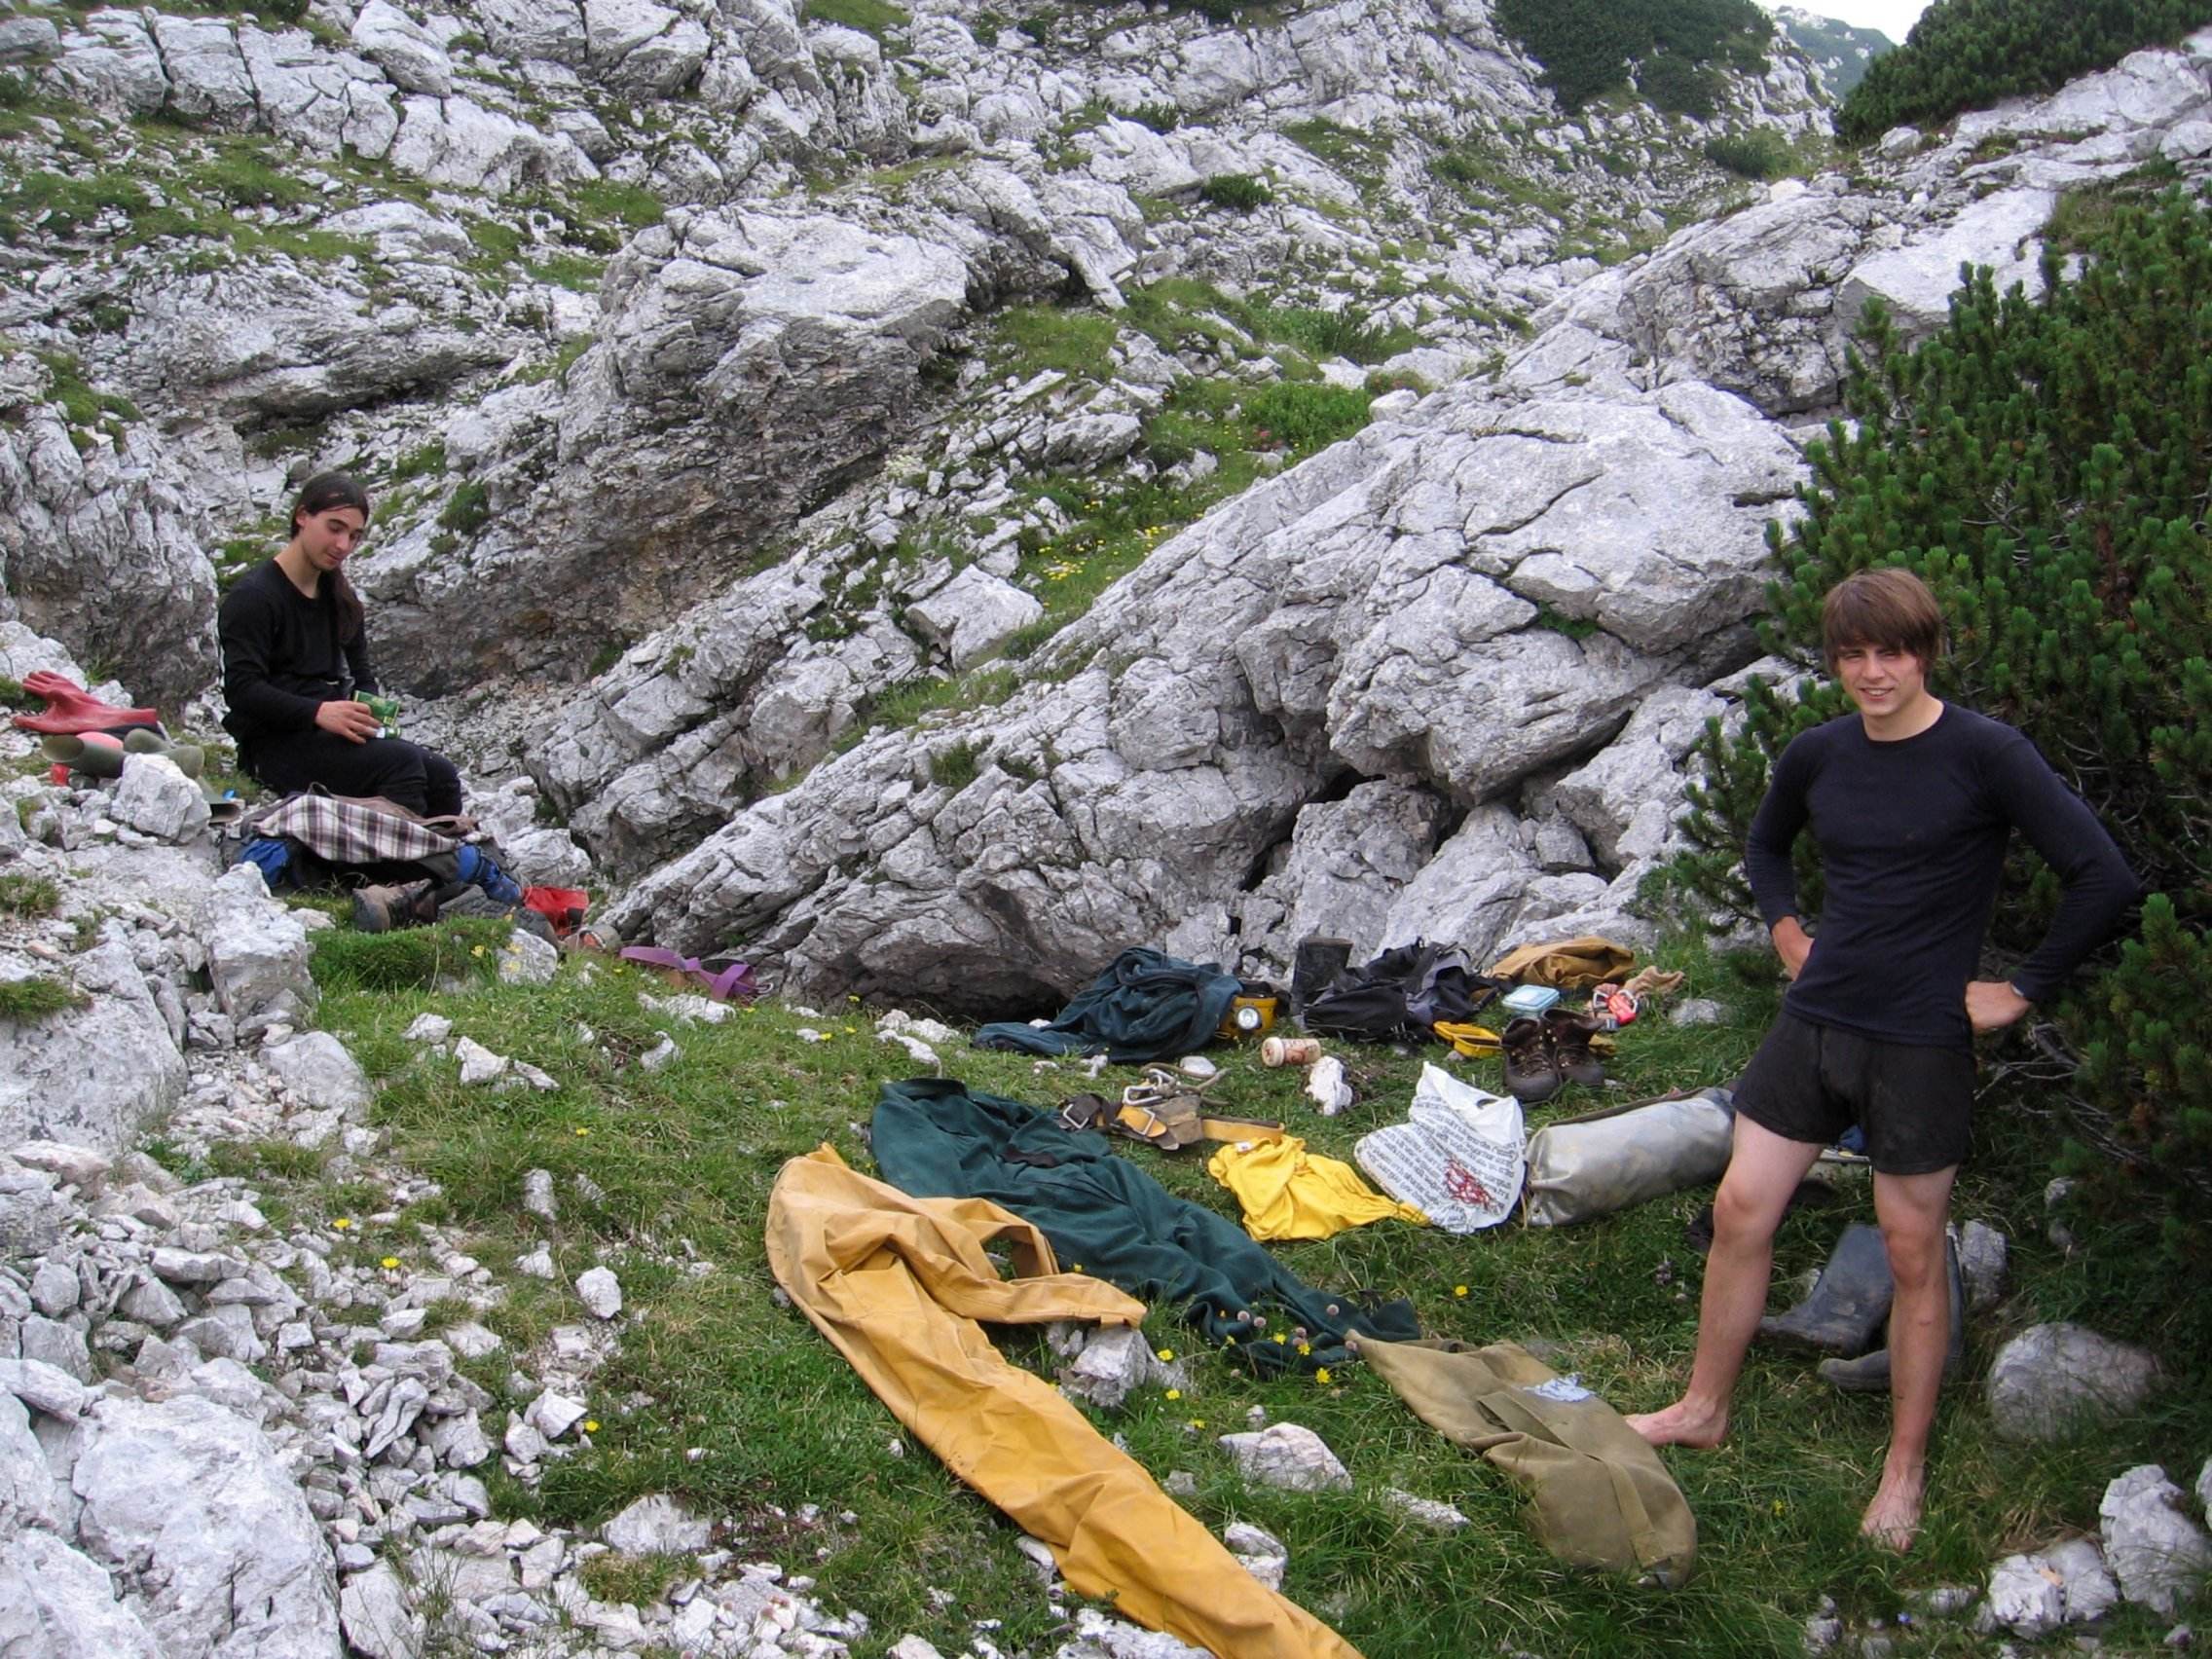
\includegraphics[width=\linewidth]{2008/vilinska/Jarvist Frost - canon a520 - gw - ck team getting ready at entrance to gw--orig.jpg}}
\caption{Izi and Paul getting changed at the entrance of \protect\passage{Gardeners' World}. \protect\passage{Vilinska Jama} was connected to \protect\passage{Gardeners' World}, becoming the second entrance to the larger cave. \pic{Jarvist Frost}}
\end{figure*}

\section{Vilinska Jama AKA Tetley's mysterious lead}

Tetley led the way down past \passage{Gardeners' World}, only grudgingly agreeing that blindfolds would not be required. The entrance is an unwelcoming yet
strangely inviting scree slope under a bedding plane, with a howling and
glacial draft emerging from it.

We headed down, leaving Janet at the surface to see off any would-be
unsurpers of the joys within. The way on quickly opens up to a chamber
with a snow plug then regresses just as quickly to a tight, boulder
filled, rift. Tetley started chiselling away at a constriction. Dan took
over while Tetley dug underneath, bypassing the squeeze entriely. More
up \& down around the boulders led to an impassably tight pitch head.
Tetley \& Dan made slow progress with chisels until Bozo arrived, having
extracted our location from Janet. A few mighty blows later, the way on
was clear (still tight though - will need more destruction).

\tweet{10:16AM Jul 31st, 2008}{GW now system with con of VILINSKA to bot of laurel.}

Tetley rigged a ladder from a securely wedged boulder, and Dan clambered
down into a boulder strewn chamber. Water was dripping from a crack in
the ceiling, and the rift continued ahead. 

``Does it go?'' shouted
Tetley. 

``Game on!'' came the reply.

Bozo forged ahead, quickly finding another chamber, filled with a vast
two way boulder slope. Up and over choked quickly. Down and under was
precarious in the extreme, but Tetley's careful progress under the
hanging death and down a short climb yielded the next pitch. A
$\approx$ 20 m drop into a large fault controlled chamber. With no
SRT kit or rope we made our exit, pausing briefly to discuss potential
names. We settled on \passage{Vilinksa Jama} (Veela cave) and returned to the \passage{Bivi}
for Tea \& Medals. 

\name{Dan Greenwald}

\begin{figure*}[t!]
      \checkoddpage \ifoddpage \forcerectofloat \else \forceversofloat \fi
      \centering
    \begin{subfigure}[t]{\textwidth}
    \centering
        \frame{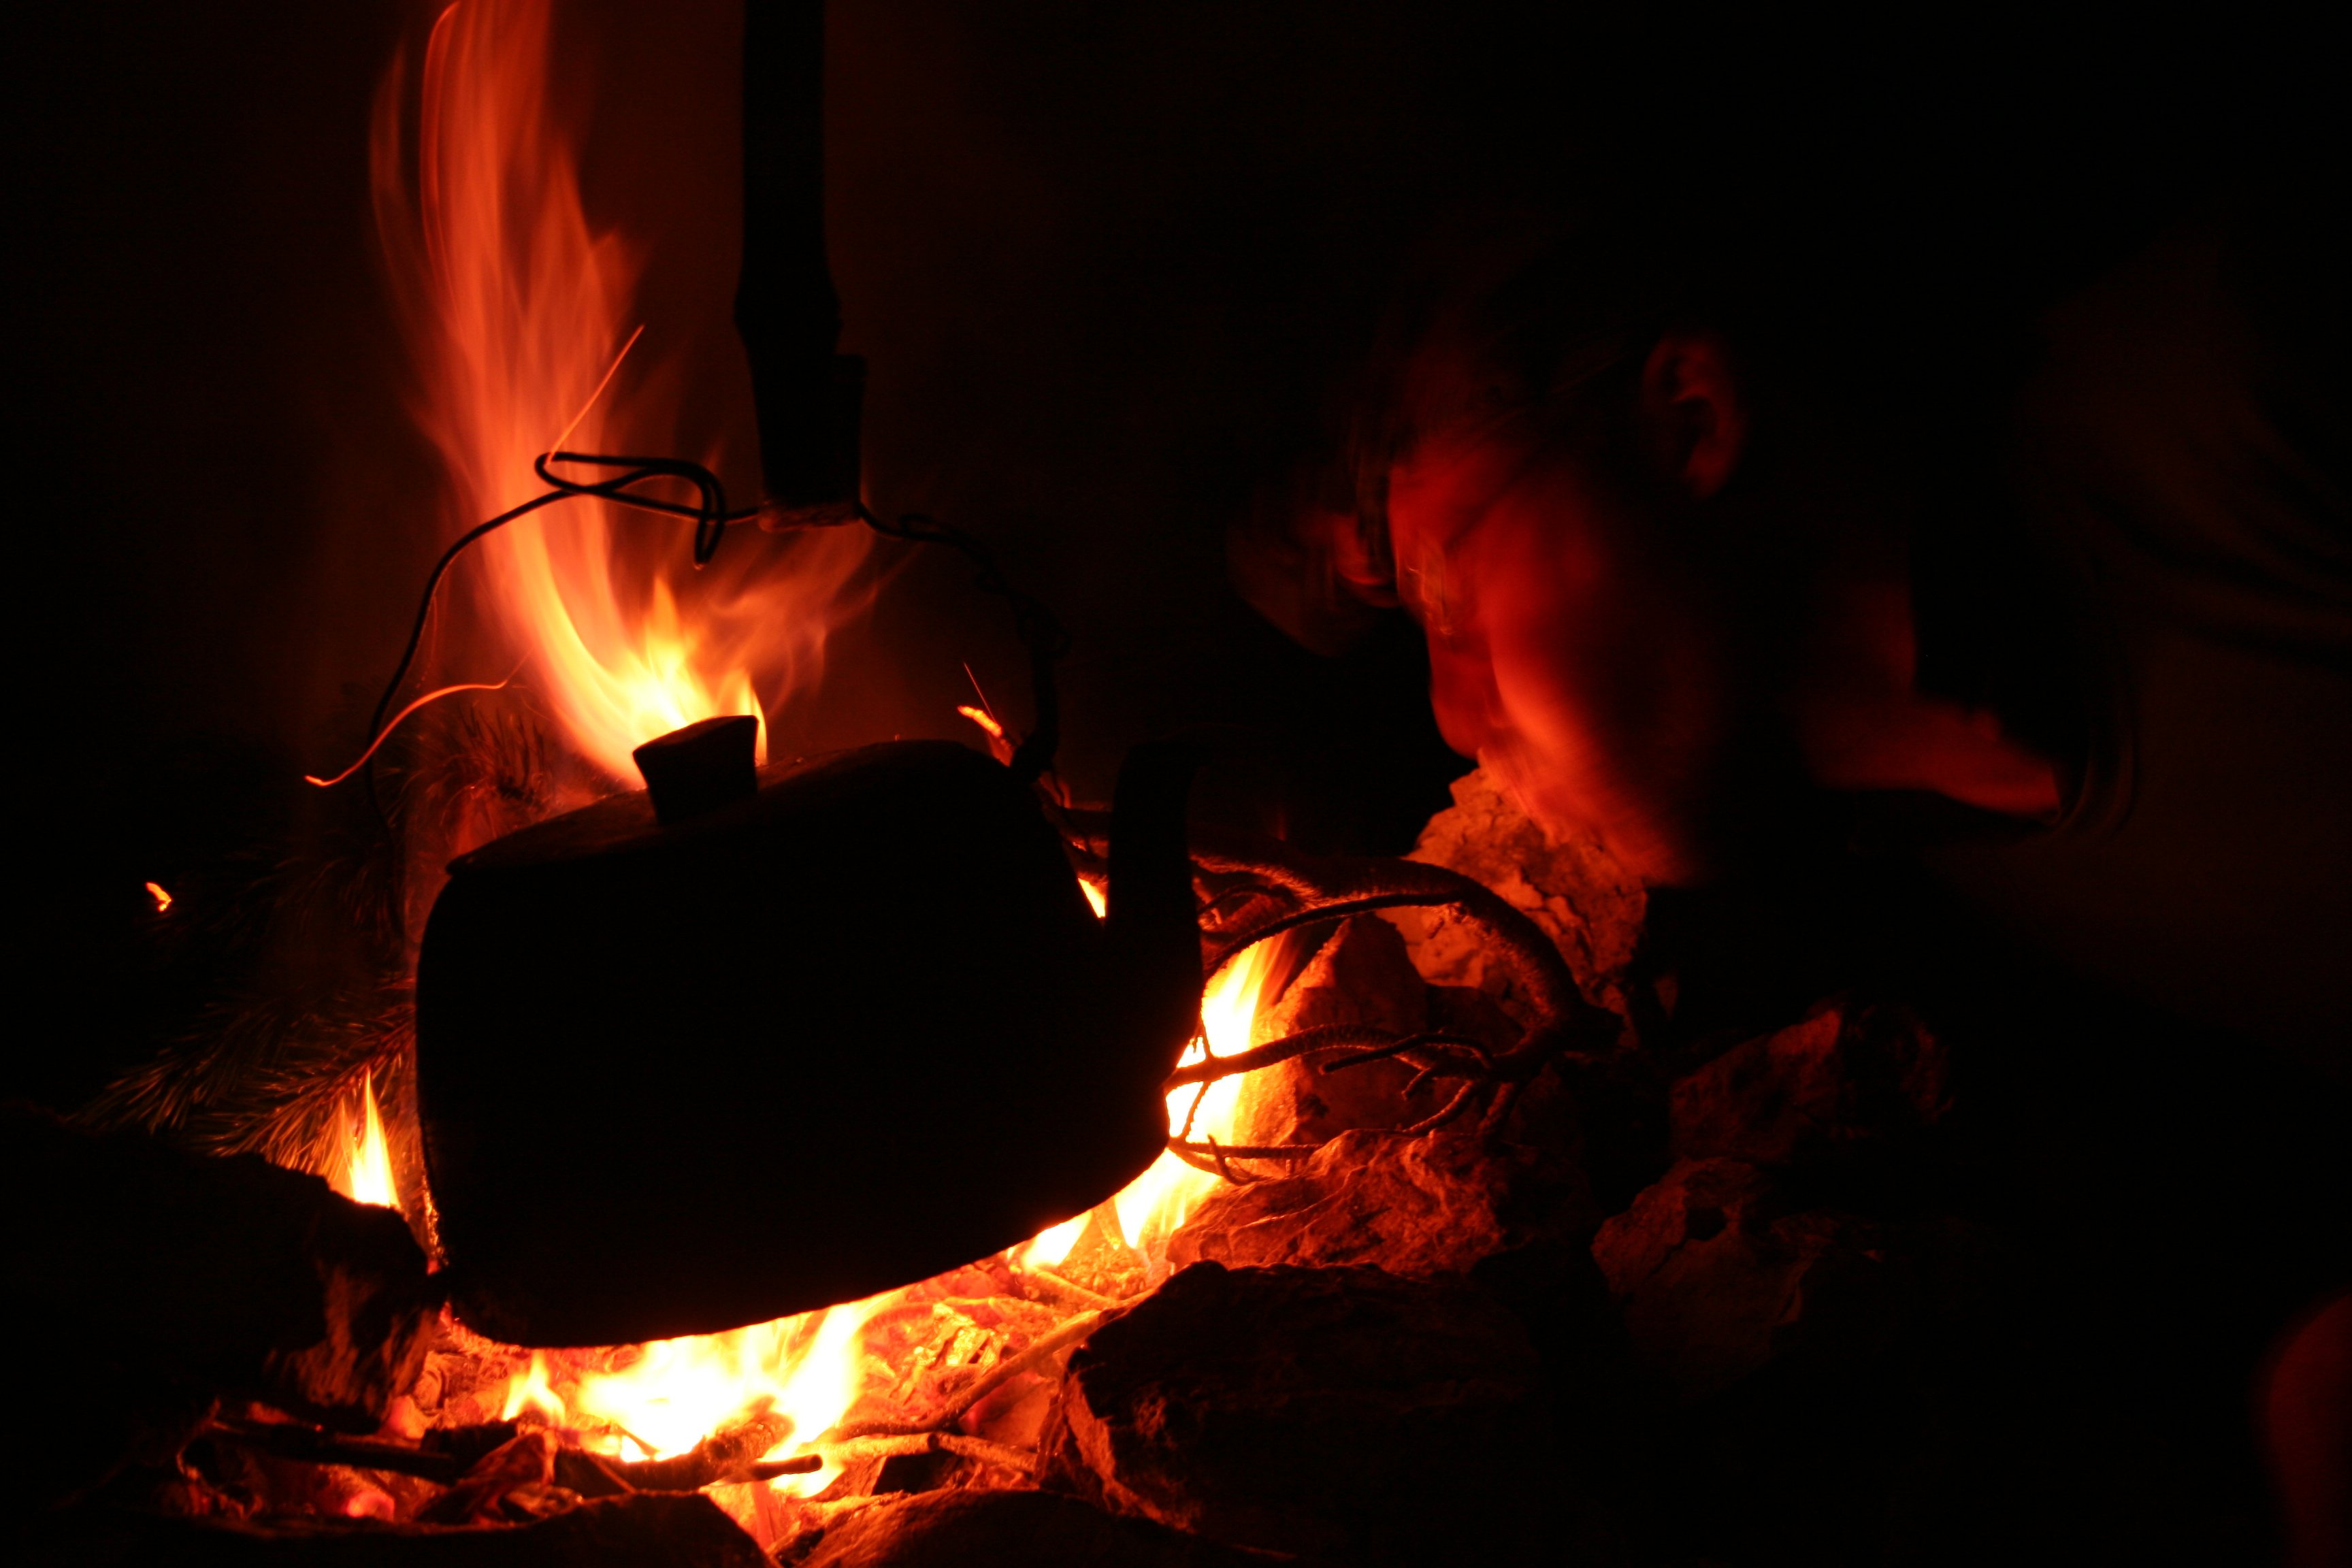
\includegraphics[width=\linewidth]{2008/vilinska/Jana Carga - Canon 350D - img_3115 tetley blowing the fire to brew tea--orig.jpg}} 
        \caption{} \label{tea bivi}
    \end{subfigure}
    
          \vspace{0.3cm}
          
    \begin{subfigure}[t]{0.49\textwidth}
        \centering
        \frame{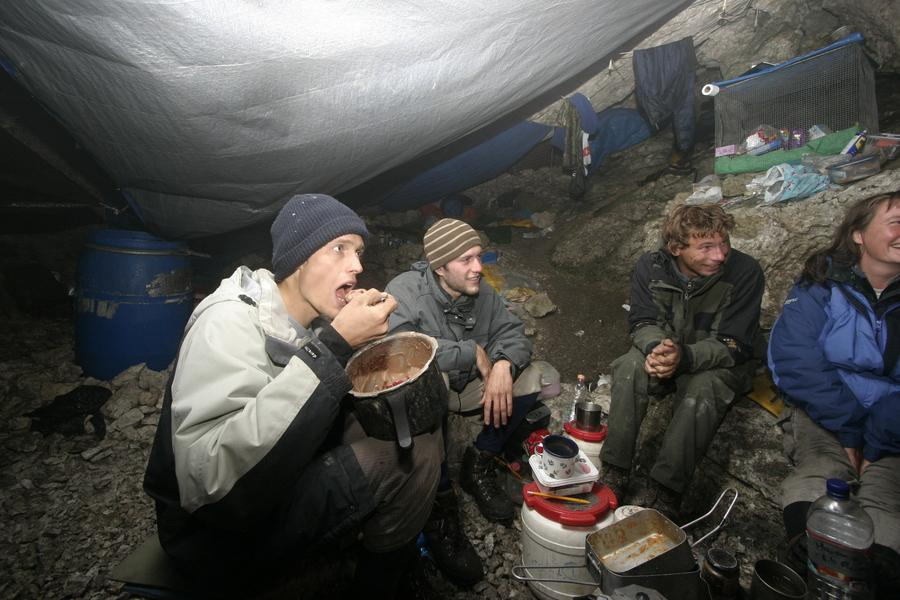
\includegraphics[width=\linewidth]{2008/vilinska/MMslov08 58--orig.jpg}} 
        \caption{} \label{jarvist anal}
    \end{subfigure}
    \hfill
    \begin{subfigure}[t]{0.49\textwidth}
        \centering
        \frame{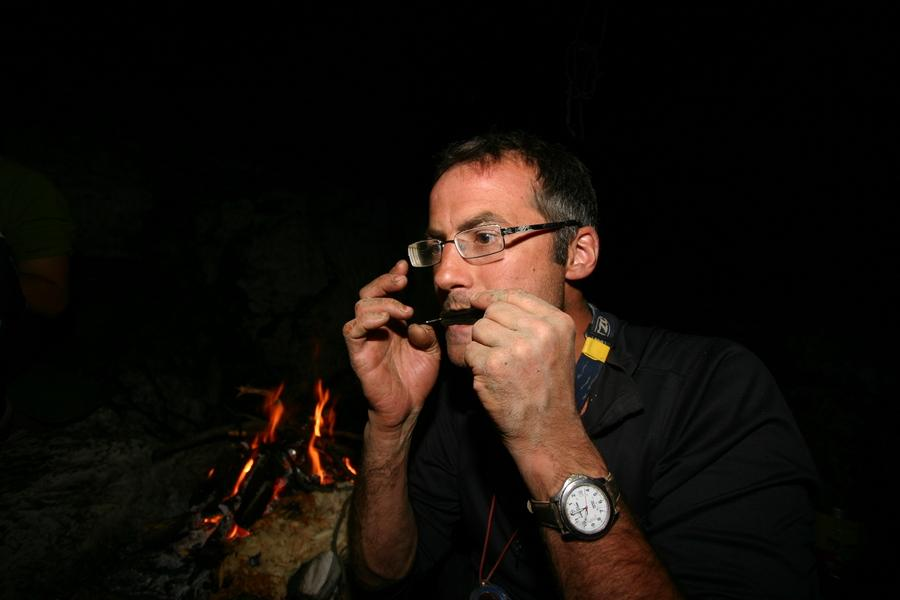
\includegraphics[width=\linewidth]{2008/vilinska/MMslov08 29--orig.jpg}} 
        \caption{} \label{tetley jawharp}
    \end{subfigure}

    \caption{Bivi nights.
    \emph{(a)} Tea in the bivi. \pic{Jarvist Frost}   \emph{(b)} Angel delight, which is made (and eaten) communally by handing around the pan and a whisk and beating the mixture until you tire and pass it on, is a beloved evening pudding.
    \emph{(c)} Tetley's musical instrument of choice in 2008 was the jawharp. \pic{Martin McGowan}}
\end{figure*}
\section{\texorpdfstring{Trying to climb into
\emph{M2}.}{Trying to climb into M2.}}

\begin{quote} Incompetence, bravery and no luck. \end{quote}

Our main aim in 2008 was to discover the connection between \emph{M2}
and \emph{Gardeners' World}, a feat which would heap honor on the
shoulders of who discovered it. 2008 was my first year of caving in
Slovenia and I was \textit{very keen}. I dreamed of my shoulders baring
the honor of the great discovery and did all I possibly could to be on
the right trip at the right time. I took part in a few of the rigging
trips down \emph{M2} and was amazed by alpine caving on Migovec: the
truly huge pitches, the dry nature of the caving, could not wait for
more ``pushing''. At the time, the Bivi rumour machine had determined
the most likely way to find the connection was to explore the area
around \emph{Kill'em All} in \emph{Captain Kangaroo}. This side branch
of \emph{Vrtnarija} had been pushed the previous year by Rik and was
infamous: uncharacteristically tight and twatty, rigged sparsely and
badly, a total nightmare.

My first pushing trip in \emph{Captain Kangaroo} was with Clewin. The
deeper you get into \emph{Captain Kangaroo} the more ridiculous the
rigging was, with plenty of dodgy climbs waiting to dislocate your
shoulder or break your ankle. The cherry on the cake was at the time
\emph{Kill'em All}, the most insane piece of rigging I have ever been
exposed to.

The pitch head is at the end of a tight rift. The original rigging
consisted of a Y-hang in the main shaft, roughly half a meter below the
entrance rift. The only way to get on the rope was to clip in and drop
on the rope, possibly with a forward roll. The only way to get out was
to clip the Y-hang with long cows tails, stand on the knot, wedge
yourself into the rift and unclip. In retrospect criminally dangerous
and terrifying, but at the time I thought this must be ``expedition
rigging'' and took it in my stride. On the way out we bumped into Jarv
and Paul who had rerigged large sections of the cave making it safer, by
the end of the year the cave was more or less sensible. On that day
Clewin and I pushed the main lead down, rigged two small pitches. I had
my first taste of caving exploration and I loved it. Game on!

The trip with Clewin had already brought the bottom of the cave too deep
for the expected position of the closest point to \emph{M2}. I had
somehow developed a reputation as a `climber' and decided to have a go
at climbing into a side passage at the top of \emph{Kill'em All}. This
required an easy slabby climb halfway up the pitch. We added a bolt half
way down the pitch from which Gergely belayed me. In order to protect
the climb I had some very long 8 mm rawl bolts, a rock pecker and a
bunch of slings. I had had tried out the rock pecker on the surface, but
found it much less easy to use whilst climbing, hammering away, the legs
a bit weak with fear of falling, footholds feeling precarious in the big
wellies, feeling I would knock myself off the wall\ldots{} I bottled it,
abandoned a very poor bolt, slung a sling around a spike and free
climbed the short slab. A very easy climb (maybe Mod?) but nevertheless
terrifying. I think that Gergely's singing helped a lot. At the time it
felt like a great achievement. But it did not lead to the connection.

Climbing with a rock pecker was too scary, so the next time Izi and I
took an electric drill. It weighed a hell of a lot going through
\emph{Captain Kangaroo}, but it would make climbing the traverse above
\emph{Primula} a walk in the park. Unfortunately once we arrived, the
drill would not work. Bogus. Plan B: hammer in a spit and belay me
across. This also failed, due to the rock being very rotten. Plan C: use
a natural for the belay and then free climb. While Izi slung some
boulders and backed up to the rope above, I scoped the climb. Doable.
There is a sort of foothold halfway along but it is total commitment --
a long step. The traverse was on the limit of the delicate climbing that
can be done in full caving gear, I reached the rift at the far end of
the traverse, wedged myself in and hammered the fastest spit I have ever
placed. Once secure, I considered the way on. The rift was going
slightly up and was totally blocked. No way on. But another crap
inducing climb, and another step to make me less Keen!

The highlight of that years caving for me was actually a trip in the
bottom of \emph{Captain Kangaroo} with Izi. On that trip we discovered
\emph{Dark Tranquillity}. It was the first proper pitch I pushed and the
buzz was incredible. I remember sitting at the top discussing with Izi
how it would rigged. I was apprehensive of screwing up, but he made it
clear he trusted me.

Somehow the expedition ends.

\begin{enumerate}
\def\labelenumi{\arabic{enumi}.}
% \tightlist
\item
  I am not upset at not having found the Connection.
\item
  I am glad that I had some fun pushing trips.
\item
  I am grateful I did not get hurt, or hurt my caving partners.
\item
  I am proud of having another person trusting me.
\item
  I am now a lot less Keen, know a thing or two about Bivi rumours. But
  it would take a few more brocken drill carries to make me wizen up
  electrically!
\end{enumerate}

\name{James Kirkpatrick}

\section{Discovering Dark Tranquillity}

 \margininbox{Dark Tranquillity}{
     \begin{itemize}
    \item James Kirkpatrick
    \item Iztok Možir
    \end{itemize}}{\explo}

\begin{marginfigure}
\checkoddpage \ifoddpage \forcerectofloat \else \forceversofloat \fi
\centering
 \frame{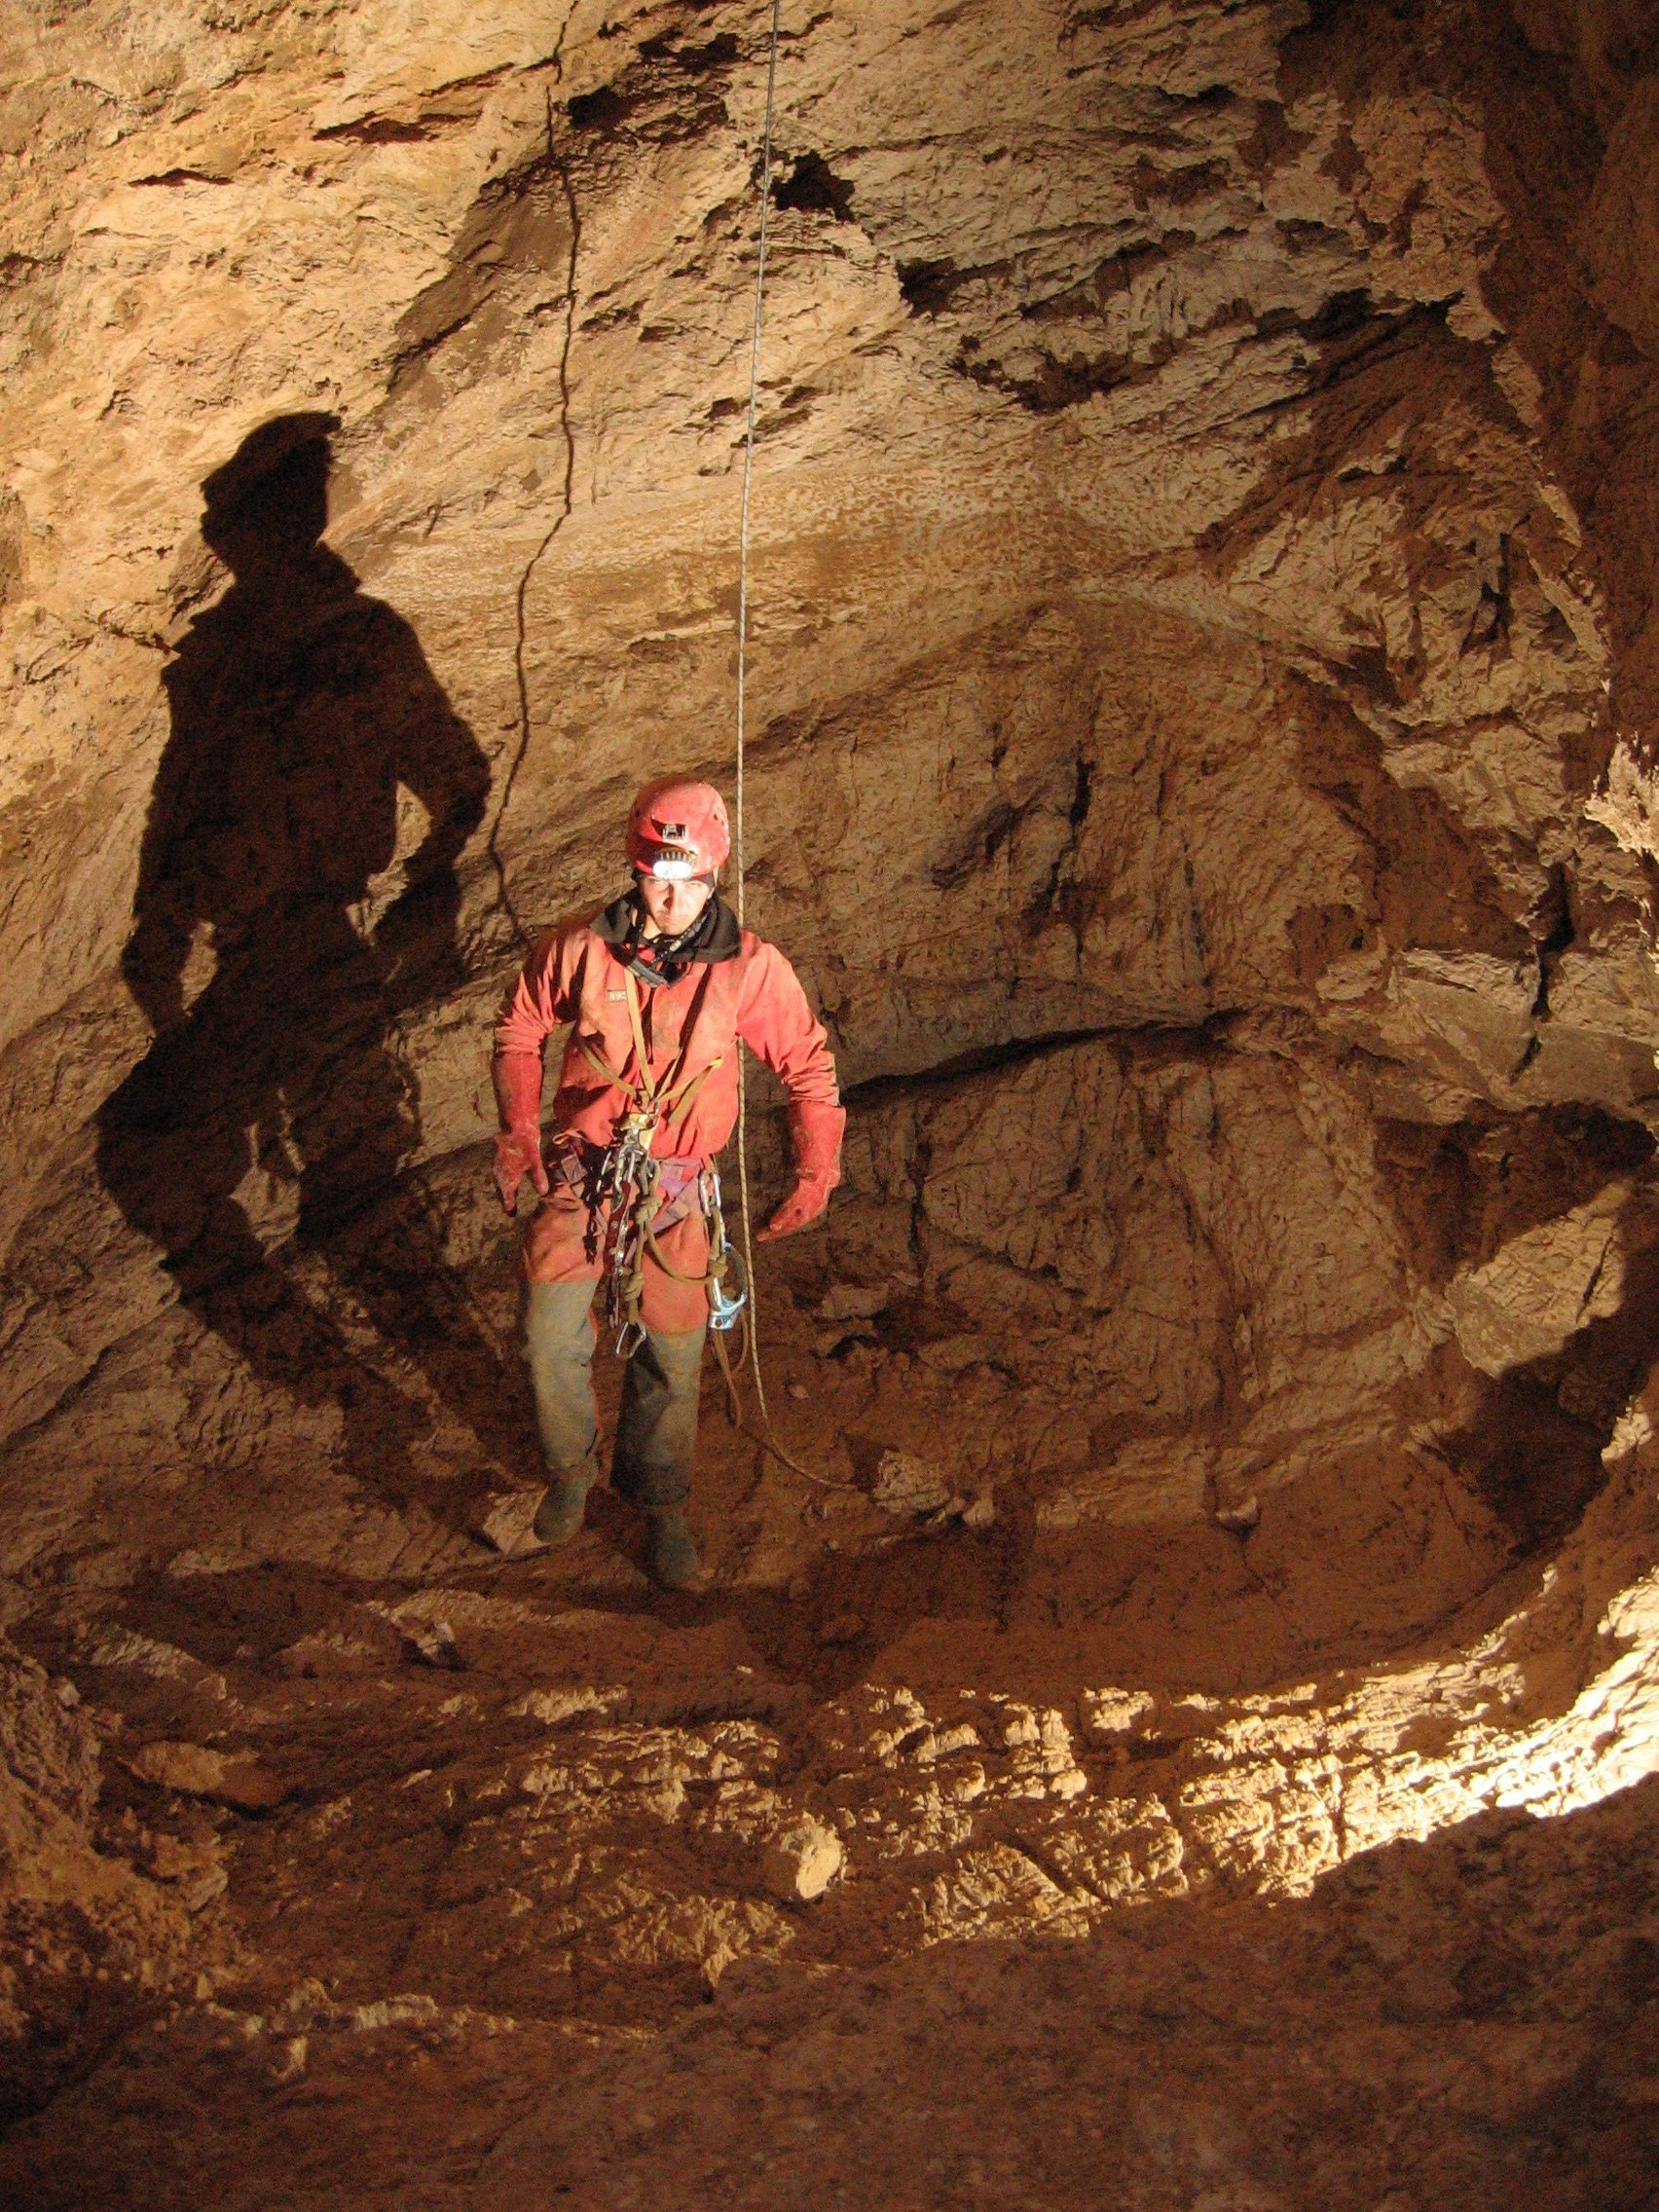
\includegraphics[width=\linewidth]{2008/tranquility/Jarvist Frost - canon a520 - gw - ck traverse chamber izi arriving--orig.jpg}} 
 \caption{Izi in \protect\passage{Traverse Chamber} in the \protect\passage{Captain Kangaroo} branch. \pic{Jarvist Frost}}
 \label{traverse chamber}
\end{marginfigure}

One year passed quickly and I was back on Mig with unfinished business at the bottom of ``\passage{Kill'em All}''. There was no Rik on Migovec this year, so I teamed up with James Kirkpatrick. A plan was made and soon we were on the way. As was my tradition I smoked one before entering \passage{Vrtnarija}.

Here we were again, past a couple of pitches and a sprinkling of squeezes and we are at the top of \passage{Pico}. Before entering \passage{Captain Kangaroo} it was time for a second cigarette. This year the squeezes were much easier, as I knew the tricks to handle the
awkward constrictions. Rather quickly we arrived at the top of ``\passage{Kill'em All}'' and reached the bottom with no problems.

There we started checking out the leads and soon one of them was declared dead. Another turned out to be the way on. After short section of small meander, we ended up at the top of a large pitch. Only one bolt was needed, as there was a really nice natural. \bignote{James went down first and after about 20 m he reached a ledge. I followed down and we realised the pitch carried on}. We had to put in another bolt as the rope would rub against the ledge. James started bolting and I had time to look round as
the ledge was relatively big. We noticed windows on the side and naturally thought that this could be the way to \passage{M2}. We did not have any climbing equipment, so we had to continue downward. Soon we arrived to another pitch. We did not have any more rope with us at the
time, so we had to turn back. While surveying we noticed how beautiful the pitch was. We named it \passage{Dark Tranquillity}.

Once in the Bivi, we were given a well deserved dinner and Jarv was
already on the mission to enter the data. The bottom of \passage{Dark
Tranquillity} was heading towards deep parts of \passage{Vrtnarija} --
towards \passage{Friendship Gallery} in fact - and unfortunately it proved
already to be low to connect to \passage{M2}.

\name{Izi Možir}


\begin{survey}
\centering
\frame{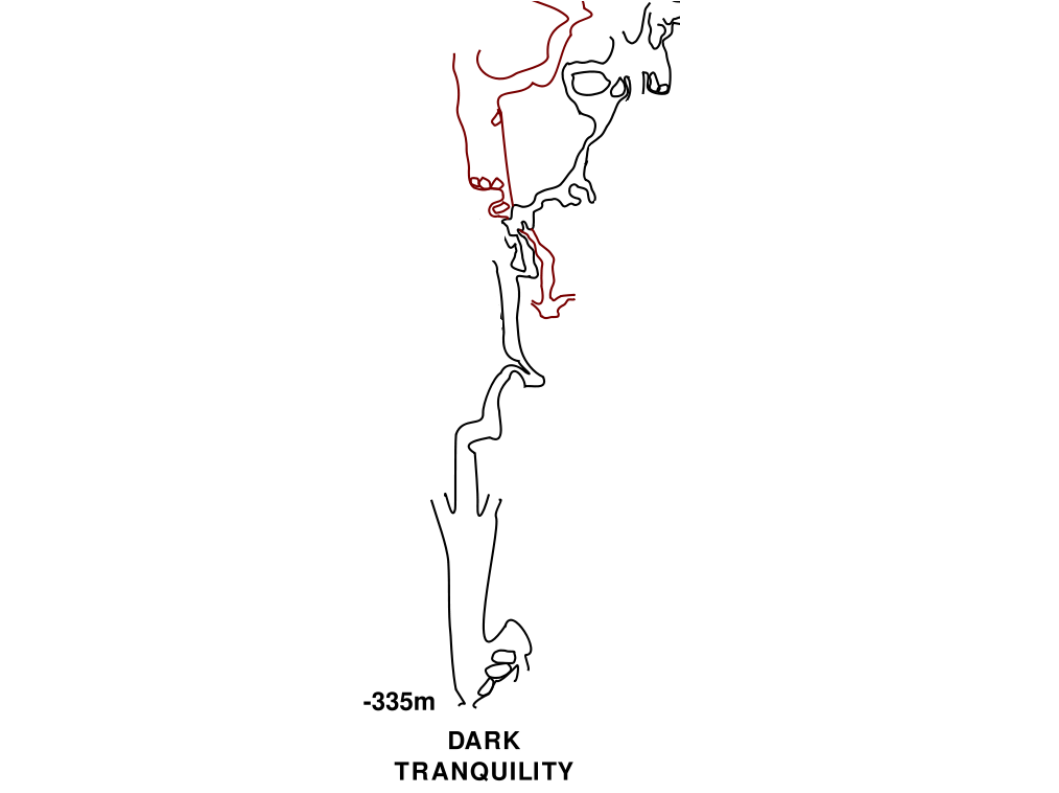
\includegraphics[width=\textwidth]{2008/tranquility/dangermouse1_bcra_2008.pdf.png}}
\caption[Dark Tranquillity]{Survey of \passage{Dark Tranquillity}, juxtaposed with pitches in \passage{M2} in red.}
\label{Dark Tranquillity}
\end{survey}



\begin{pagefigure}
\centering
\frame{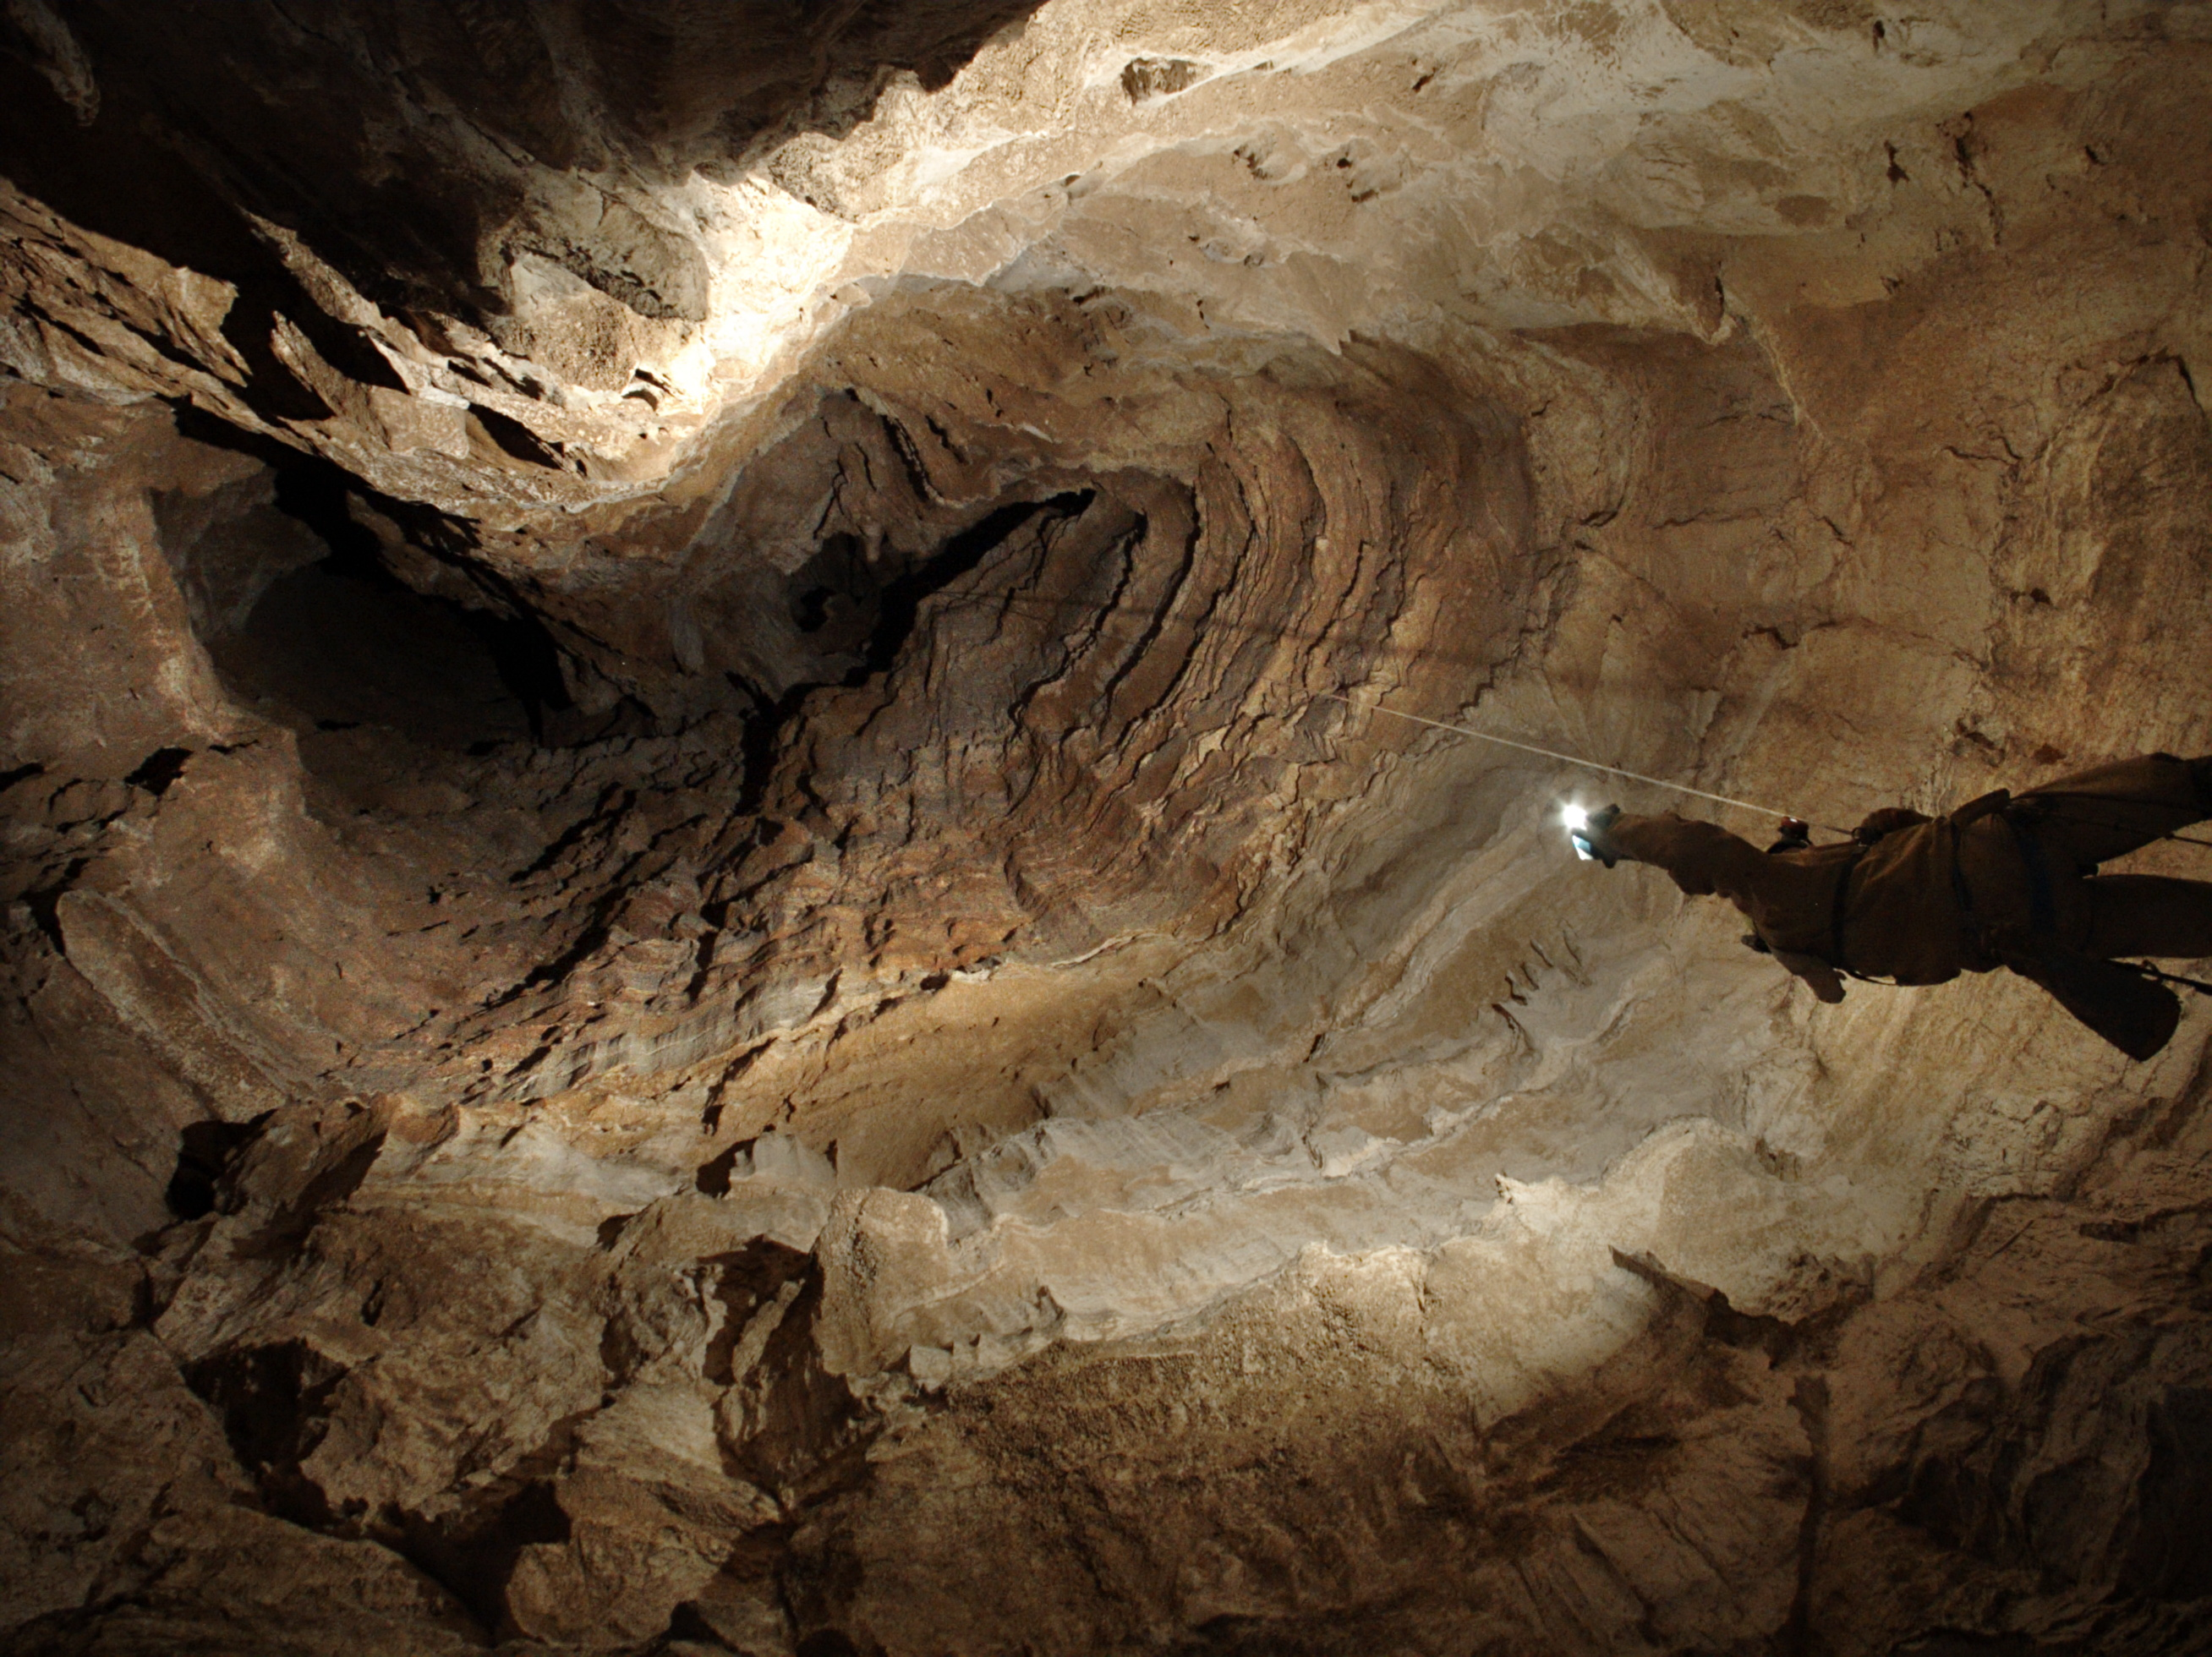
\includegraphics[width=\textwidth]{2008/tranquility/2009-08-10-18.26.08 - Jarvist Frost - Canon Powershot G5 - dark tranquility - gergely 8 odd metres from ground single vivitar 283 flash--orig.jpg}}
\caption{\protect\passage{Dark Tranquillity} pitch, with Gergely Ambrus in 2009. \pic{Jarvist Frost}}
\label{Dark Tranquillity pitch}
\end{pagefigure}


\subsection{28.07.08 - Surface Work}

\begin{marginfigure}
\checkoddpage \ifoddpage \forcerectofloat \else \forceversofloat \fi
\centering
 \frame{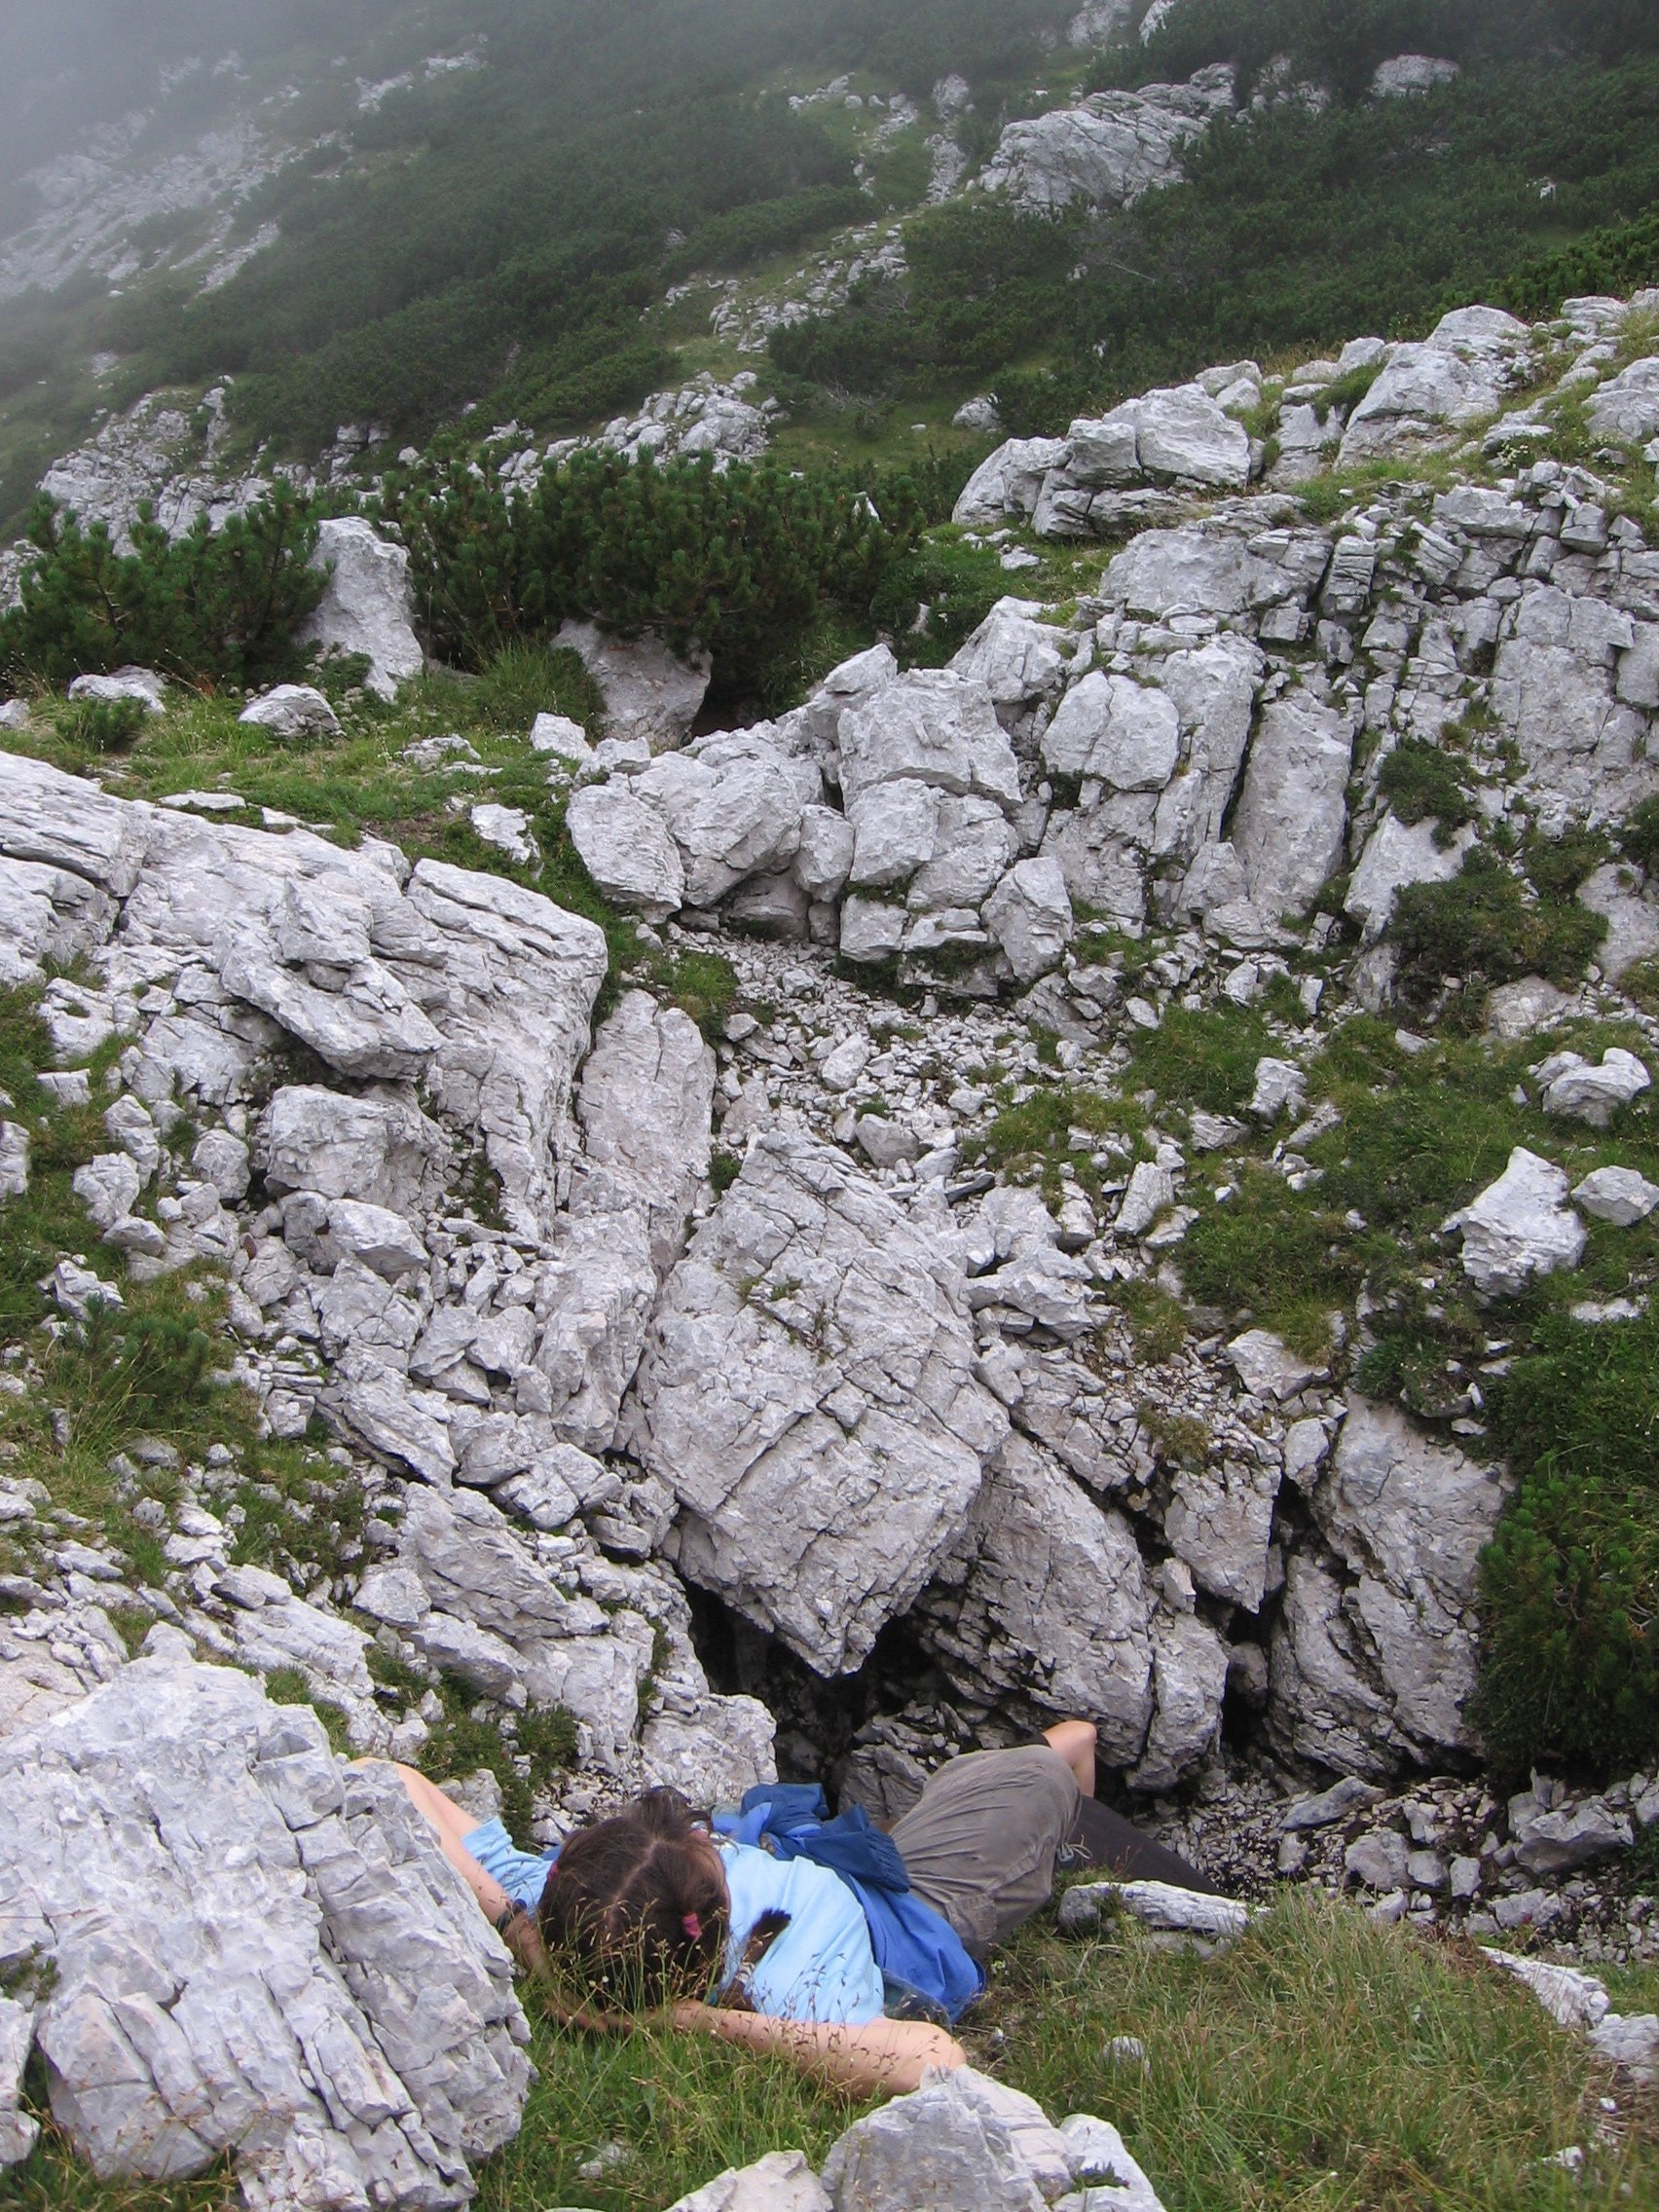
\includegraphics[width=\linewidth]{2008/surface/Jarvist Frost - canon a520 -janet lounging near new cave on plateau below mig--orig.jpg}} 
 \caption{Janet demonstrates the pleasures of surface bashing. \pic{Jarvist Frost}}
 \label{janet relax}
\end{marginfigure}




\begin{enumerate}
\def\labelenumi{\arabic{enumi}.}
% \tightlist
\item
  Went back to Valley 8 (next one to \passage{B9}), you can see loads of cave
  entrances. Check out. But only one goes. You climb down under the
  boulder choke, turn right down to a small chamber. From here there are
  at least 2 ways on. They both require the removal of boulders. All to
  be done very gently and carefully since so many blocks hang on top,
  but otherwise looking good to go.
\item
  Behind \passage{M19} have noticed a small cave entrance. A slope down to a
  chamber visible. Did not go down, since at that time I was alone. Put
  a cairn to mark an entrance.
\item
  East of \passage{M19} possibly next to \passage{M15} - There is a big
  entrance. We climbed down and digged (a bit) 3 possible routes on.
  Quite draughty. On to the bottom way on(?) we noticed that someone
  might have used a hammer. You can feel a lot of cold draught. Digging,
  smashing, needed but it does look very good to go!
  \sidenote{JCC GPS Waypoint 1851 m N46.25311 E013.7610}
\item
  Loads of big (deep) entrances just behind the Bivi. Almost of them
  have snow at the bottom. Rope needed to explore!
\item
  Re-discover the \passage{Royston Vasey} (we believe?) re-located.
  \sidenote{See Hollow Mountain I, p. 147}
\item
  Re-discover, located a cave entrance with a red spot in front. It
  starts with a narrow pitch down. Next to red spot it is an old bolt as
  well. It is just further on on the right up from \passage{Royston Vasey},
  looking towards \passage{Kuk}. Worth going back down again. (We believe this
  is Dave Wilson's 1996 Dig\sidenote{See Hollow Mountain page XXXXXXXXXXXXXXXXXXXXXXXX})
\end{enumerate}

\name{Jana Čarga}

\fullwidthbox{30-07-08 Jana, Andy, Janet → Surface Work}{

    Jana, Andy and Janet collected the GPS coordinates of all large holes in the area of the Bivi.
    
    They checked the 'M'holes (\passage{M1}, \passage{M16}, \passage{M18}, \passage{M4}, \passage{M15}, \passage{M17}, \passage{M19}), and added new entrances, (\passage{A1} to \passage{A4}), all of which are worth a quick 'go down' and 'look'.
    
    Bolting kits needed!
    
\name{Jana}
}

\section{Intravenus de Milo and a Captain Kangaroo diatribe}

 \margininbox{Intravenus de Milo}{
     \begin{itemize}
    \item Clewin Griffith
    \item James Kirkpatrick
    \end{itemize}}{\explo}

After plenty of trips down \passage{M2}, it was time to push the other side
of the mythical \passage{Gardeners' World}-\passage{M2} connection. James KP
\& I caved down to \passage{Traverse Chamber}, past \passage{Captain
Kangaroo}. Originally I thought that the \passage{Gardeners' World} side
would be more pleasant than \passage{M2}, but then the repressed memories
of \passage{Captain Kangaroo} resurfaced as the passageway turned into a
succession of horrible squeezes, horrible climbs and horrible pitcheads.



Traversing across \passage{Traverse Chamber} and into \passage{Mudslump}, the cave quality declined somewhat, decaying into crumbling climbs and pitches which had been rigged off a dodgy natural, half way down. We pushed on, hoping to find a PSS with ``\passage{Kill'em All}'' written on it. Eventually we did. Relief was rapidly followed by shock and despair when James crawled around the corner and saw the \passage{Kill'em All} pitchhead. To paraphrase him at the time: ``This is by far and away, and without a shadow of a doubt the worst and most contemptible pitchead you'll ever see.''

%He wasn't far off. Schematically it looked something like this: (diagram OKAY DON'T FORGET TO REMOVE THIS FIONA HOPEFULLY THERE WILL BE A DIAGRAM BUT IF NOT)Coming up would certainly be a problem, but we were going to be exiting via \passage{M2} through the as-yet-undiscoveredconnection, so we didn't consider that eventuality.% 

He wasn't far off. Coming up would certainly be a problem, but we were going to be exiting via \passage{M2} through the as-yet-undiscovered connection, so we didn't consider that eventuality.

\begin{marginfigure}
\checkoddpage \ifoddpage \forcerectofloat \else \forceversofloat \fi
\centering
 \frame{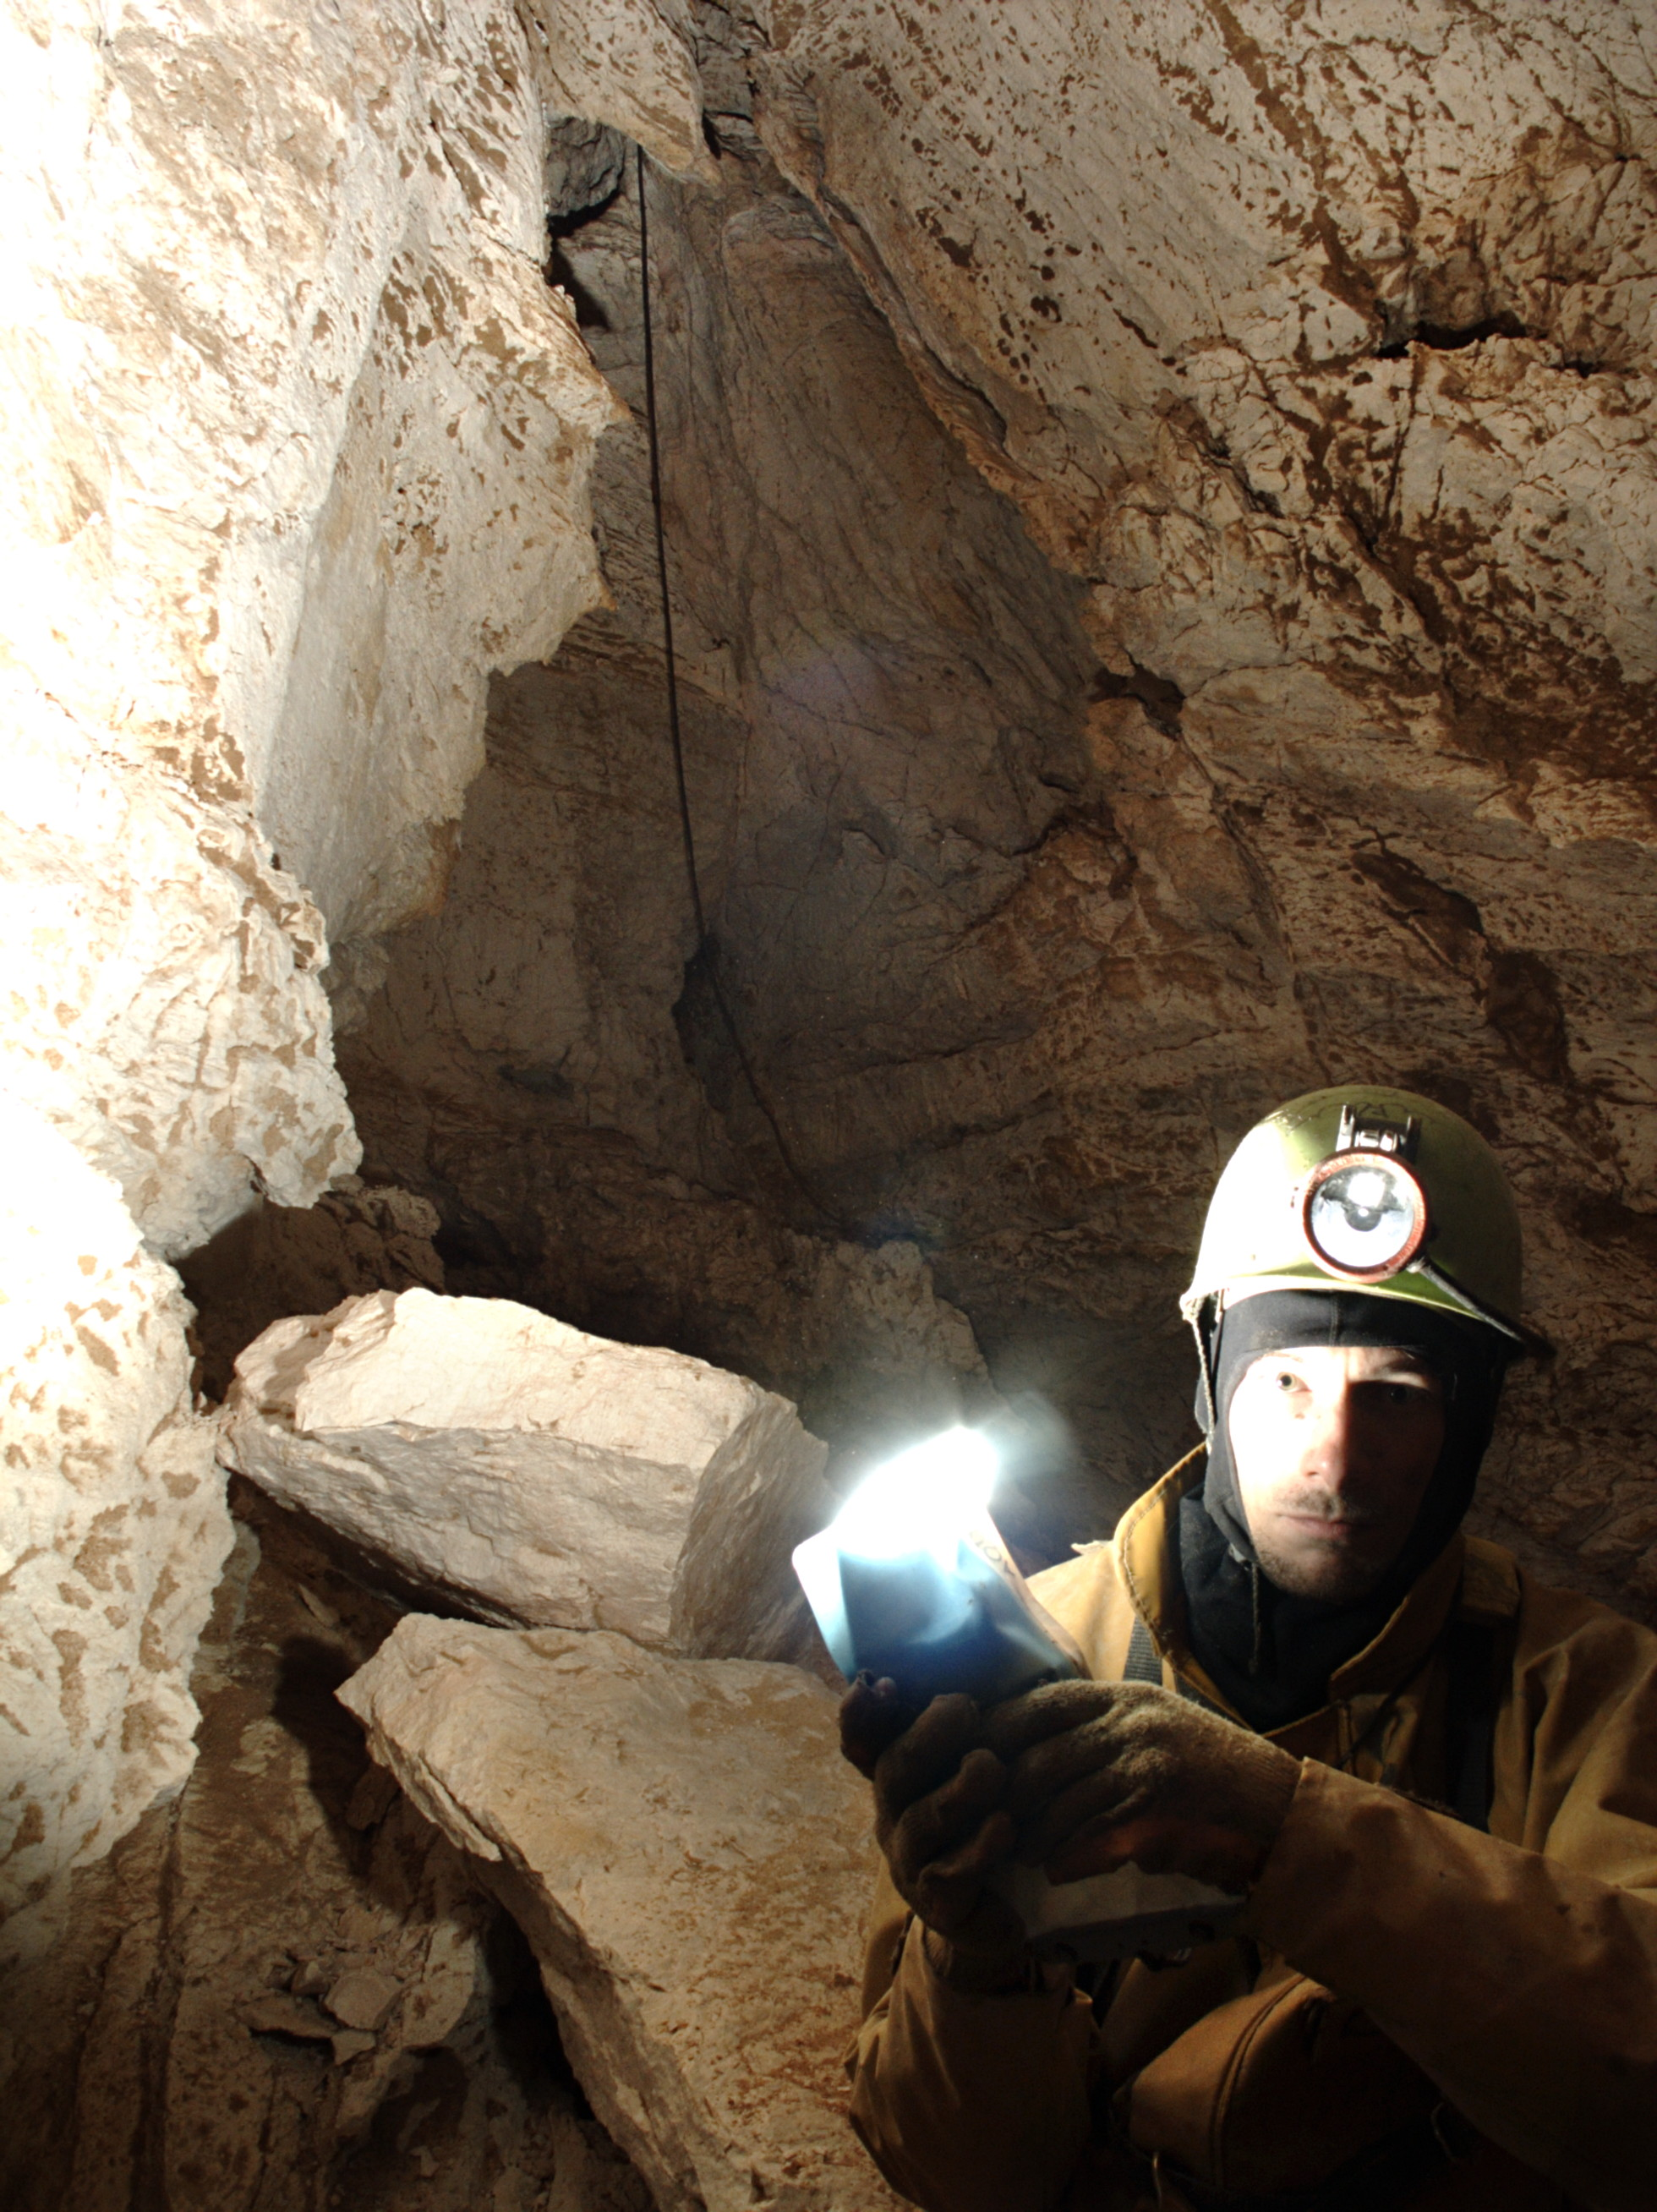
\includegraphics[width=\linewidth]{2008/intravenus/2009-08-10-18.05.38 - Jarvist Frost - Canon Powershot G5 - intravenus de milo chamber - gergely--orig.jpg}} 
 \caption{Gergely Ambrus in \protect\passage{Intravenus de Milo} chamber in 2009. \pic{Jarvist Frost}}
 \label{intravenus chamber}
\end{marginfigure}

Compared with the unspeakable \passage{Mudslump}, the cave at the bottom of
\passage{Kill'em All} pitch was actually quite nice. There was a climb down
near the bottom of the pitch which we attempted, before the dawning
realisation that rescue after a fall here would be pretty much
impossible. So we rigged off a natural and dropped to the floor. I sat
and smirked as James struggled to get even his helmet through the
miniscule rift at the bottom. So that lead was dead. We derigged and
turned our attention to the only other way on, the rift leading south
from the bottom of the pitch. The rift zigzagged left then right and we
climbed up into a round window on the right.

This lead to a small pitch. I belayed James down and he found a rift at
the bottom leading to a pitch with a ``5 second'' drop. He then revised
that down to 4 sec. I'd suggest 35 m (maybe 2 ½ sec). I put a bolt in
and dropped down so we could survey out.

 \margininbox{Kill'em All 30/31-7}{
     \quote{\textit{The problem wasn’t so much the rigging was bad, as that there was no rigging at all.}}
     \mininame{Jarv, Izi, Paul, James} }{\logbook}

The \passage{Intravenus de Milo} pitch looked really pretty, with horizontal
blades of rock jutting out at various levels. By the time we had
finished surveying, we were running short of time -- 4 hours to our call
out. The way out was fairly desparate, with me getting stuck on climbs
and James stuck in squeezes. No one bit of cave was truly awful, but the
combined effect of 3 solid hours of unrelenting scrot of the purest
variety on the way out started to sap my will to live. Having grit in my
wetsocks grinding away at my toes didn't improve the experience. Still,
got out with 2 mins to go before our callout.

Back in the Bivvy, superb slop and trifle for dessert was really
appreciated. Shockingly, despite my recounting tales of squalor, four
people were eager to go down the next day. Such is the lure of
exploration I guess.

\name{Clewin Griffith}



%(Large multi coloured Grade I of \passage{Mudslump} - \passage{Kill'em All})

%James Kirkpatrick's first grade 1 survey: \passage{Dark Tranquillity} Many curious avens on pitch.

%Followed on from \passage{Intravenus de Milo} development. James KP

\section{Plopzilla Photo Trip}

\margininbox{Plopzilla}{
     \begin{itemize}
    \item Jarvist Frost
    \item Andy Jurd
    \item Paul Hutton
    \end{itemize}}{\explo}

Andy's last trip; so it had to be \passage{Plopzilla}.

Set off with a Daren drum of gear, with Paul in the lead and Andy
bringing up the rear (Ooh-err!). Took a few firefly digital shots coming
up into \passage{Hotline}. Seems to be lots off the lower \passage{M16}
entrance series, such as pitches into \passage{Lost City}, etc.

More photos on the newly sexy \passage{Gladiator's}\sidenote{\texorpdfstring{\passage{Gladiator’s traverse}}{Gladiator’s traverse}} rigging, then shot off up
\passage{Fawlty Towers}. Popped into \passage{NCB}; Andy conned us into
pissing down \passage{Silos}:- ``Don't piss in the main passage, climb down
there but no further than the first bolt!''


\begin{marginfigure}
\checkoddpage \ifoddpage \forcerectofloat \else \forceversofloat \fi
\centering
 \frame{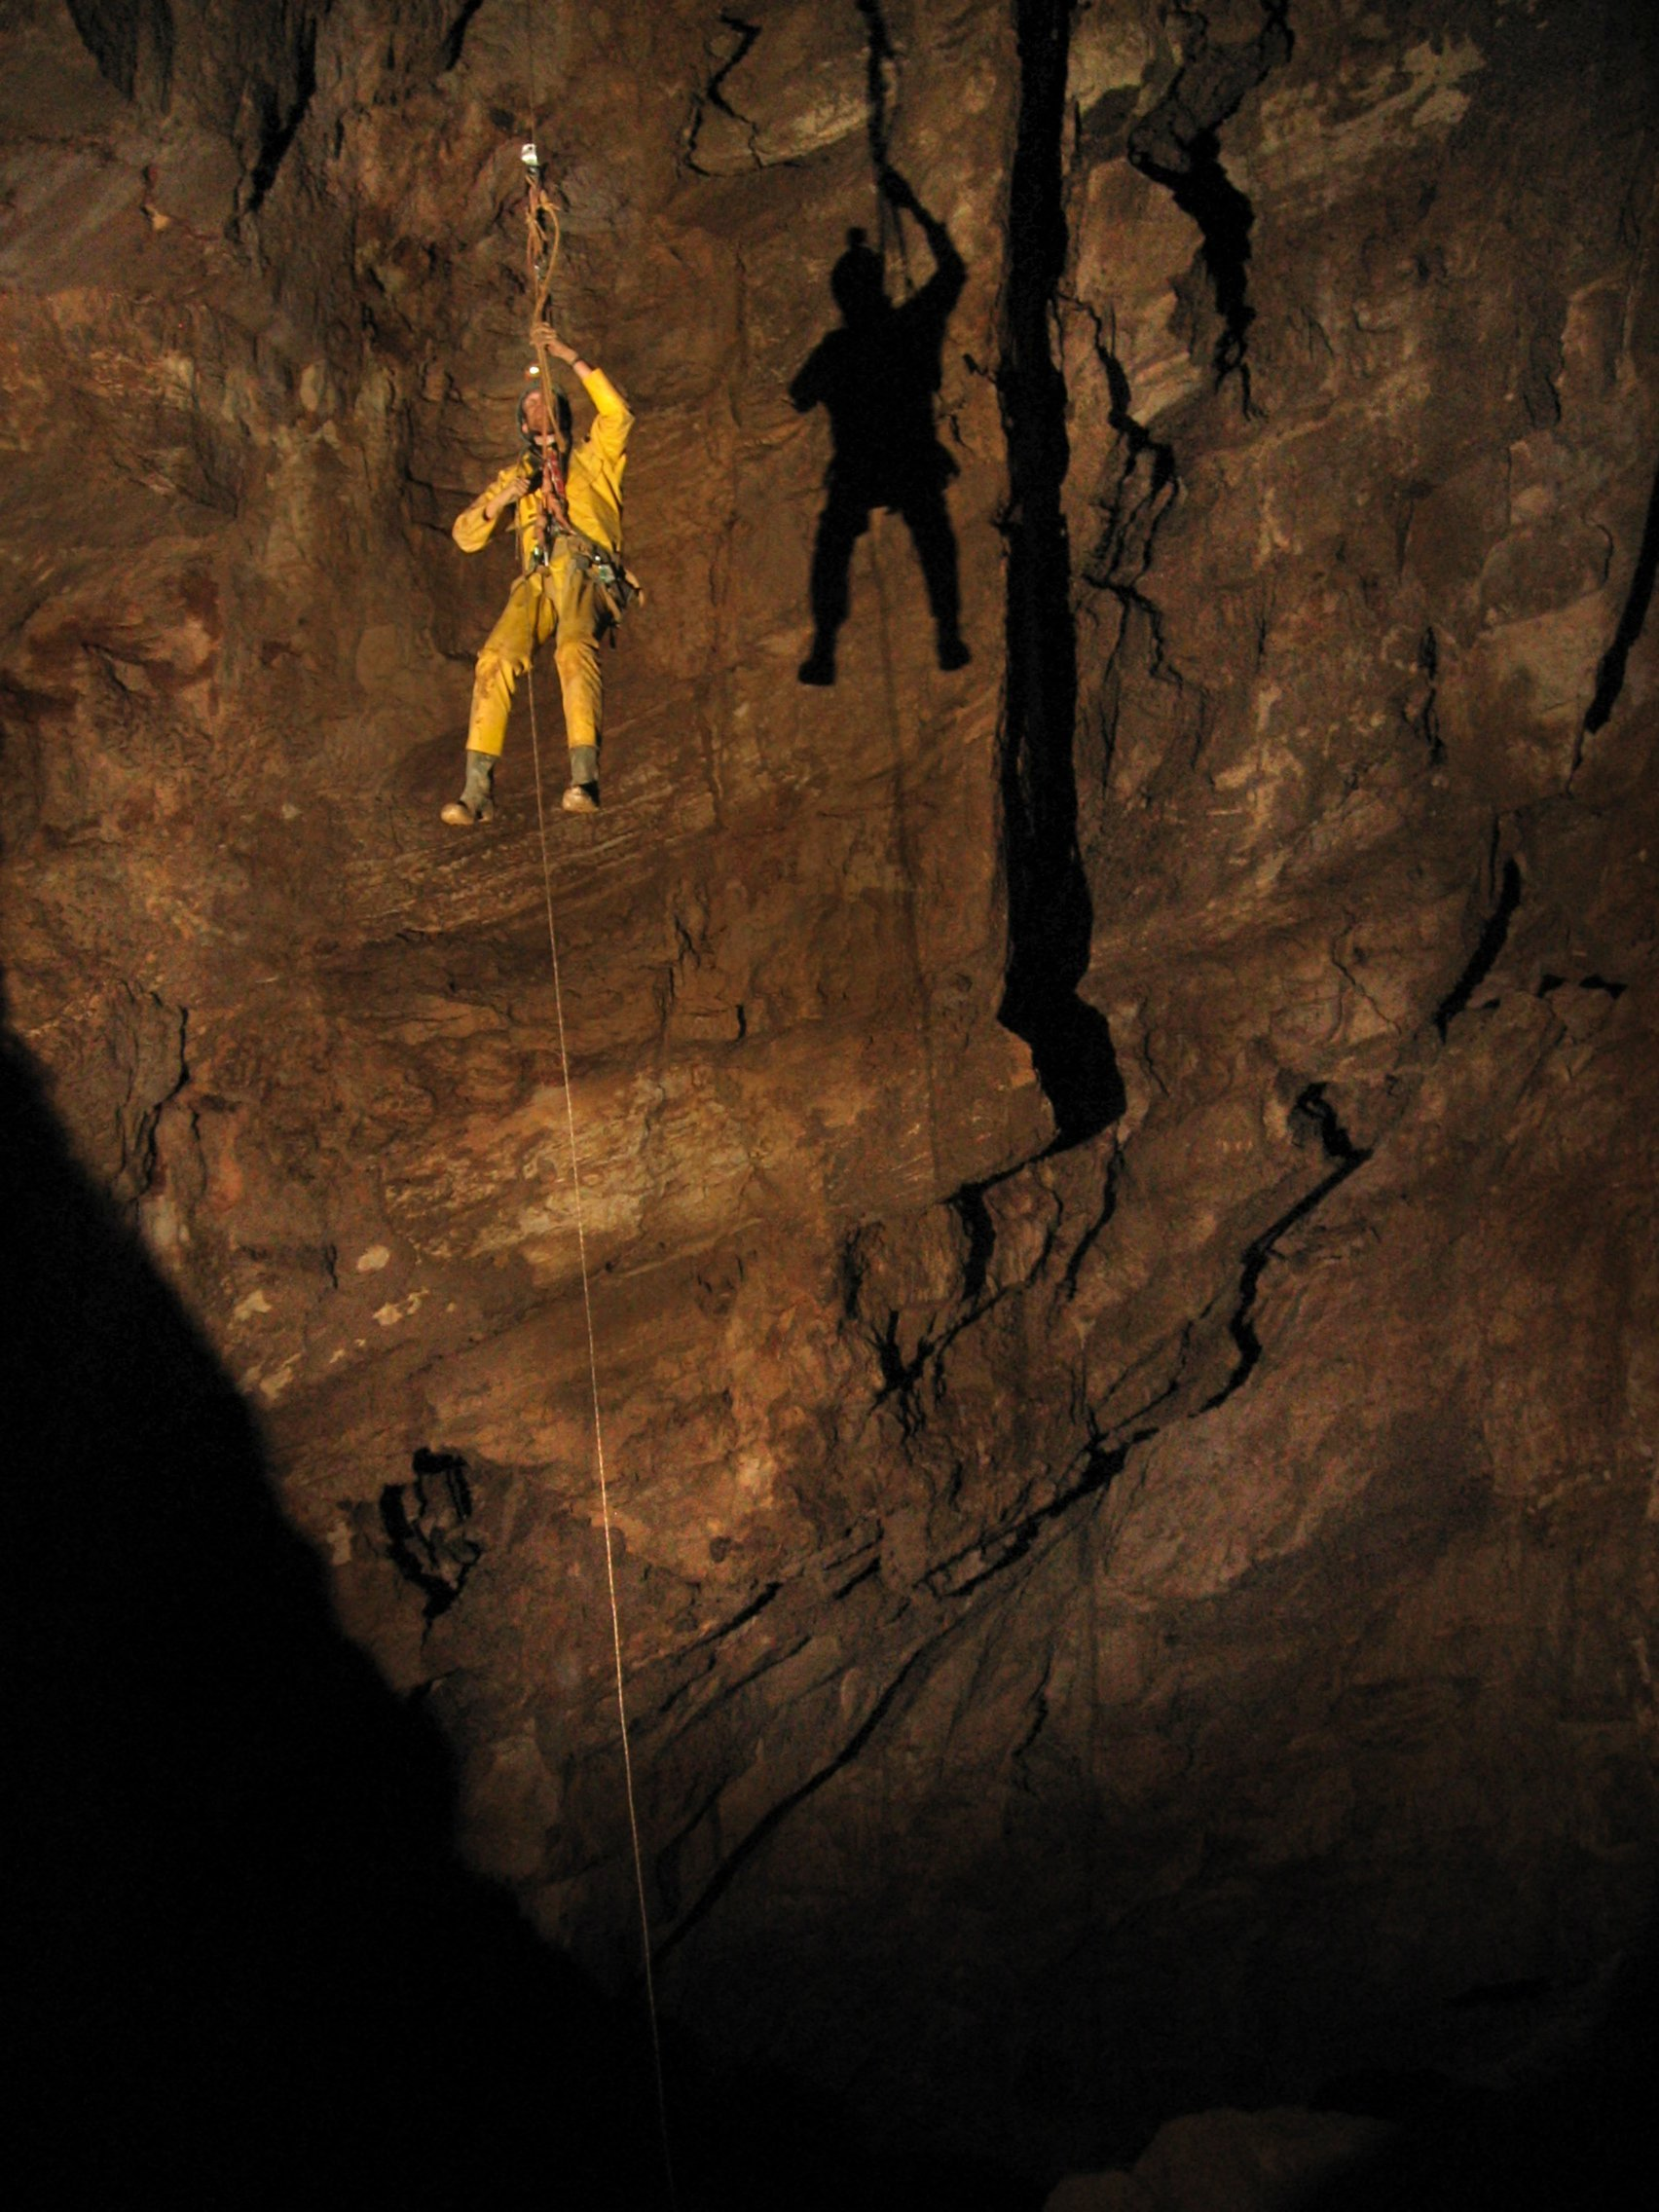
\includegraphics[width=\linewidth]{2008/Plopzilla_photo_trip/Jarvist Frost - canon a520 -plopzilla - andy 9mm knot pass b--orig.jpg}} 
 \caption{\protect\passage{Plopzilla} knot pass \pic{Jarvist Frost}}
 \label{paul plopzilla}
\end{marginfigure}


Rerigged traverse in \passage{NCB} (more photos!), then to the main game:
\passage{Plopzilla}. We had a plan, I asbeiled down with gear \& scrambled
up a slope. Pitch head was `interesting' (clip in cows, push through
squeeze and swing out above the 105 m drop hoping cows were still in).
Rebelays were `interesting' (so tight, one had to climb above belay to
derig descender). Knot change `exciting' (knot a `Rik Special' - 9 mm
below super slippery). Gear down there `intriguing'
\sidenote{this explains where all the rope went, 90 m 11 mm, 90 m 9 mm and 1 tacklesac}.

We tried our best on 2 attempts at filming exploration, a few digital
pictures, and then dived into the Boulder choke. Went down -30 m or so,
drips, went through a lot of very loose Boulders then into bigger
stones, but with solid wall, lots of Boulders. Many drips, no stream
hearable. Otherwise very similar to \passage{Jelly Chamber}. Got as far as
a loose committing climb into a large-ish chamber.

It goes, it really does. But I'm not going there. Stones rattled
\textasciitilde 4 seconds.

Climbed ridge to corner and found another entry to choke.

So we left \& derigged. Rope → Club Mig. Sped out once, gear stashed.
2hrs from bottom to \passage{Fawlty Towers}.

\name{Jarvist Frost}


\begin{figure}
\checkoddpage \ifoddpage \forcerectofloat \else \forceversofloat \fi
\centering
 \frame{\includegraphics[width=\textwidth]{2008/Plopzilla_photo_trip/Jarvist Frost - canon a520 -ncb - andy fixing traverse to plopzilla closeup--orig.jpg}} 
 \caption{Andy Jurd alters the rigging on the traverse at the head of \protect\passage{Plopzilla} \pic{Jarvist Frost, assisted by Paul Hutton}}
 \label{Plopzilla traverse}
\end{figure}
\section{The Slov magic}

 \margininbox{M2}{
     \begin{itemize}
    \item Gergely Ambrus
    \item Andrej Fratnik
    \end{itemize}}{\explo}

Shortly after arriving to the plateau, I found myself getting ready for
a trip. Not only a trip, in the ordinary sense, but a real Exploration
Trip, with a goal none less than trying to remove the large boulder
blocking the tight rift at the bottom of \passage{M2}. I was chosen to be
the lucky one who accompanies the Living Legend of Tolmin cavers. Soon I
found myself holding a nice yellow tacklesack, with the instruction of
``be gentle with it''.

And this was not without reason. In the bag there was to be found an
original memento of the great war, a product of the ever famous factory
in Glasgow, dated to 1937. A well educated friend of mine pointed out
later, that products bearing the name of a prestigious prize become
highly unstable in a period of circa 50 years, but little of this
reassuring fact had I known back then. Instead, I took the tacklesack
happily and we started our vigilant journey towards the centre of the
globe.

\tweet{9:43AM Aug 5, 2008}{Super action today to try and push the sysmig/GW connection. Change of man power after the weekend, now more slovs on top. 15hr+ trip!}

It soon became evident that the only way for being faster than my master
would be to use gravity directly, without the unnecessary complication
given by ropes, re-belays and so on. The main obstruction was a nasty
wedging squeeze somewhere, which proved to be even worse on the way out.

Finally, we reached the bottom, set up our magical set, murmured a
couple of magic spells, and then woops, the boulder evaporated as if it
had never been there! Indeed, it does help in exploration to read Harry
Potter after all. We started to chisel our way further, but the rift got
even narrower after a couple of meters, so we had to give up and started
prussiking up. Again, my companion was nowhere to be seen until I
emerged completely exhausted at the bottom of \passage{Silos} -- where he
waited half asleep, and noted that he is indeed quite cold. It was just
the opposite for me. The rest of the trip continued in the same manner,
and finally we emerged triumphantly at the surface. \bignote{This was my first
battle with \passage{Migovec}, and so to say, I got completely addicted to the
sweet smell of gunpowder}.

\name{Gergely Ambrus}

\section{\texorpdfstring{\emph{Dangermouse}}{Dangermouse}}

\begin{verse}
He's the greatest! He's Fantastic!\\
Wherever there is danger he'll be there!
\end{verse}
\name {Dangermouse}

\margininbox{Dangermouse}{
     \begin{itemize}
    \item Jarvist Frost
    \item Izi Mozir
    \item Paul Hutton
    \end{itemize}}{\explo}

\tweet{6:53 AM Aug 6th, 2008}{GW:JF/PH/IM new big pitch DANGERMOUSE off mudslump.Attempt at vocal con,no joy.}

With a load of food \& bolts, we shot down to \passage{Something Fishy} \& dived
down the right crawl. Drafting, with deep sand floor (all spoiled!).
Became rather tight after \textasciitilde7 m.

So we hit the pitch, belay off jammed boulder, soon with a bolt.

Paul \& Izi set off to grab the 2nd bolt kit. Hopped down 2nd pitch (6
m) and came to something seemingly identical. Rigged off obvious natural
\& dropped down to choosy shelf \textasciitilde8 m. Then I turned
around. Small pitch it was not. Boulders banged for 6s+. Water could be
heard a long way down, nothing visible (not even a drip!). The way
to the \passage{M2} confluence?

From -25 m (limit), one could peer down past cascades into\ldots{}
blackness. Big chamber?

Left \textasciitilde50 m of 10 mm at last bolt, PSS on sticking-out
ledge + bolt kit. \& 2nd bolt kit at head of \passage{Something Fishy}.

Early exit \textasciitilde1AM.

We blew trumpets every hour \& listened every x 30 minutes - nothing
from the \passage{M2} crew.

\name{Jarvist Frost}

\section{Scrotty Bashing - Martin, Paul,
Tim}

After the last trip, it was quite clear that the passages in
\emph{Captain Kangaroo} needed some alterations. So over a few drinks
and the fire I talked about the possible home improvements we could
make. The idea of bashing the shite out of scrotty seemed to appeal to
lots of people, no doubt motivated by the idea of getting something back
on the annoying part of the cave.

So Paul, Tim \& I set out armed with two hammers and chisels, as well as
some tatty rope for the climbs in the cave. We were quickly down at the
start of \emph{Captain Kangaroo} and we then set about bashing the
passage. We took a cycling approach to the task with one person taking
the head of the peleton with the large hammer, then the second person
refining the passage with the smaller hammer and finally the third
person `resting' at the rear.

At Bonus chamber, Paul \& I rigged a traverse line, so you no longer
have to swing off the pitch whilst unprotected. On the same vein we made
several improvements to the handlines. The only one pitch that we could
not improve was the one that the the backup was below the main bolt. I
had removed the backup with the idea that on the way out we could rebolt
it with the kit left in \emph{Olympic Rift}.

Anyway after redecorating scrotty we listened to Bob and then headed
down for the kit left by Rik in 2007. We quickly descended the pitches
below \emph{Traverse Chamber}. It was quite clear from the offset that
this was not the normal Rik Venn rigging. It was a delight to go down
pitches with traverse lines, backups and other aspects of which would
pass for standard rigging from Alpine Caving Techniques. Well down we
went and it soon became clear that we were still in the Scrotty series
according to PSS left by Clewin. At the bottom there was a rift going
off - was this the \emph{Olympic Rift}? After a few twists and turns it
was quite clear that this rift was very tight and we were fed up with
this shit. Paul had a quick look around the corner to check that the
rift continued in the same shit manner and then we got the feck out of
there.

Overall there is a new improve scrotty, but we have no idea where Rik's
lead is from last year. Maybe looking at the survey will solve this
problem.

\name{Martin McGowan}

\subsection{\texorpdfstring{\emph{Olympic Rift} - Jarv \& Tim - by Jarv
-
12-8-08}{Olympic Rift - Jarv \& Tim - by Jarv - 12-8-08}}

From olympicrift.1, squeeze to pitch is SE, 5 m+. Wet sounding pitch
(Not Concorde?)

{[} Diagram of beyond \emph{Olympic Rift} .1 {]}

From last pitch, SW to aven (draft) + possibly over the top to pitch.
From scrotty.37, W down tight rift to ???

Squeeze is: a) Tight b) Bedrock either side c) no room for chisel Bang
ideally.

\name{Jarvist Frost}

\section{WATER!}

\margininbox{M2}{
     \begin{itemize}
    \item Gergely Ambrus
    \item Paul Hutton
    \end{itemize}}{\explo}

It was one of the last pushing trips on the expo. Once again, we decided
to go down to the unpassable rift at the bottom of \passage{M2} in order to
find the Connection. This time, for sure, it was going to happen! Paul
seemed to be as eager as I was, so we teamed up.


\tweet{10:32PM Aug 10, 2008}{\protect\passage{S1}: way to right hand pitch found by hammering rift above big pitch.Strong draft from tight meander, several hrs hard hammer.4th system?}

At the same time, another party (Jarvist and Dan) was to go down to the
``other side'' of the rift, to hear our voices and then to shake hands,
for sure. So we slowly worked our way down the many tight squeezes below
\passage{Silos}, and arrived at the -- by then, familiar -- small and cosy
chamber. From here, the hammer and the chisel played the main role in
our drama, or at least we thought so.

It was not until a couple of hours later that we noticed that instead of
the usual sound of water dripping into the pool, a steady, loud,
constant noise is coming from the chamber. Squeezing back, we nervously
looked at the stream of water dropping into the pool. Time to head out,
as quick as possible! We threw some small flakes of the chocolate
tinfoil to the stream in order to find it on the other side, hastily
packed up, and started our way up, which turned out to be an ordeal. I
wore a normal textile oversuit, which proved to be perfect for the cold
water to directly run through, but Paul did not feel much better in his
Meander either. \bignote{The cave suddenly became like a wet Yorkshire cave, and
soon we were completely soaked in the icy water}.

The flow became bigger and bigger, and our only hope was that from the
top of \passage{Silos}, the way should be dry, as we have never seen water
there. Yet, once reaching the top, completely cold, exhausted,
shivering, we had the worst sight in front of us: a 40 m high waterfall,
the rope hopelessly dangling in the middle, with the majestic and
frightening sound of water as it splashes at the rocks after its long
freefall\sidenote{believe this is \passage{Kletnikov Skropilnik} AKA Kletnik's Shower}. At this point, there was no choice left: being as cold as we
were, the survival bags would have been almost useless, and the water
level seemed to rising, indicating that it is still raining on the
surface, so did we decide to wait, it would have been at least half a
day, resulting in hypothermia almost surely. We ate the last bits of
chocolate we had, jumped, rubbed our arms to get some blood going,
looked up into to dark, trying to estimate what is awaiting us. Neither
of us was sure that we were going to make it. There was a ledge midway
out of the water, so planned to go up there in one go, and then continue.

\tweet{11:16PM Aug 17, 2008}{M2:JH/JKP derig via M16, put to sleep for the year. CK:DG/TO last pushing trip to desperately seek the con, morning callout.}

Then, I clipped onto the rope. The jammers were in place, everything
sorted out, feet in the footloop, bag on the back, rope as tight as
possible. It was the moment to start. A wide swing took me directly in
the middle of the water, and without thinking, I started prussiking as
fast as I could. The force of the icy water seemed to be much stronger
than my weak, half-frozen thighs, and it was hard to get any air, like
being in the middle of a freezing icefall. I started swearing, knowing
that I had to win. Seconds seemed minutes, and minutes hours, but
finally I made it to the ledge. Paul could hardly hear the ``rope
free'', then he started up. I crossed my fingers and waited. The
gigantic howling sound covered everything, the shouts of Paul went to
thin air. \tweet{9:42PM Aug 18, 2008}{GW derigged in full, VILINSKA jama tied in. No connection, but \textasciitilde 1.2km of new cave this year, with fantastic leads for 2009! Team Mig.} Finally, he emerged with a frightened, completely pale face,
blue lips, shivering, his hands are of almost no use at all. We hugged
each other and jumped, trying to warm up. Then, the second half, just as
bad as the first. When Paul showed up at the top, we smiled a bit: from
here, we get out, even if we have to duck all the way! It was still a
good couple of hours until we made it to the surface, about 6 hours
after the callout. We dragged back to camp in the pouring rain, woke up
Tetley, drank a bit of booze, and went for a massive 15 hour sleep --
which was quite well earned after all.

\name{Gergely Ambrus}




\begin{figure*}
      \checkoddpage \ifoddpage \forcerectofloat \else \forceversofloat \fi
      \centering
    \begin{subfigure}[t]{\textwidth}
    \centering
        \frame{\includegraphics[width=\linewidth]{2008/water/MMslov08 39--orig.jpg}} 
        \caption{\textit{left to right} Gergely Ambrus, Tetley, Paul Hutton, Jarvist Frost, Izi Možir, Jim Evans. \pic{Martin McGowan}} \label{bivi jim}
    \end{subfigure}
    
          \vspace{0.3cm}
          
    \begin{subfigure}[t]{0.49\textwidth}
        \centering
        \frame{\includegraphics[width=\linewidth]{2008/water/Jana Carga - Canon 350D - img_3189 James Kirkpatrick and Clewing Griffith on start of walk up to Mig with peak behind them--orig.jpg}} 
        \caption{Clewin Griffiths and James Kirkpatrick. \pic{Jana Čarga}} \label{clewin jkp mig}
    \end{subfigure}
    \hfill
    \begin{subfigure}[t]{0.49\textwidth}
        \centering
        \frame{\includegraphics[width=\linewidth]{2008/water/Gergely Ambrus - DSLR - img_4852--orig.jpg}} 
        \caption{\textit{left to right} James Kirkpatrick, Martin McGowan, Paul Hutton, Dan Greenwald, Tetley. \pic{Gergely Ambrus}} \label{sunset lounge}
    \end{subfigure}

    \caption{Some of 2008's team members.}
\end{figure*}

\begin{pagesurvey}
\centering
\frame{\includegraphics[height=\textheight]{2008/survey/gw_m2_2008.pdf}}
\caption[2008 Gardener's World and M2 Survey]{2008 \passage{Gardener's World} and \passage{M2} Survey}
\end{pagesurvey}
\thispagestyle{endchapter}

\begin{tcolorbox}

\vspace{80pt}
	\lettrine{I}{n} summary, Migovec now has three major systems and over a dozen smaller
caves in active exploration. The exploration in \passage{Vrtnarija} was at
the very end of our endurance limits - the minimal trip length to
achieve anything was 15hrs. Our plans are to camp down there in 2009 in
order to have far more man hours at the `coal face' and to offer the
psychological and physiological refuge of a camp in a location that, in
spite of its relatively shallow depth, is truly a long way from a safe
place.

The mountain is unique in having such complicated Alpine cave formation
at various depths, and now constitutes 21.988 km of passage beneath just
a square kilometre of surface.

Everything newly explored was surveyed to BCRA Grade 4b. Underground
photography as part of documentation took place in \passage{Vrtnarija}, \passage{E1},
\passage{Plopzilla} (in \passage{Sistem Mig}) and \passage{Planika Jama}. We were limited by
there being only one underground photographer on the expedition.

A new survey on an East-West projection has been drawn of \passage{M2} and
\passage{Vrtnarija}.
 
The weekend after the expedition van headed home, a small Slovene /
English team went back down \passage{M2} armed with an enormous drill \&
battery. With 6 shot holes they blew their way through the rift, to the
head of a short pitch.

This was returned to in October 2008, and dropped - all the new finds in
\passage{M2} being surveyed at the same time. The new pushing front is
another, almost impenetrable rift, and a climb up into a series of tight
phreatic passage. The survey data indicates that \passage{M2} itself is
trending away from \passage{Captain Kangaroo}.

During the expedition a major error was discovered in our survey data - namely that the wrong \passage{M2} entrance (there are two, separated by 25 m horizontal) was connected into the surface survey. This caused a jump in the position of the bottom of \passage{M2}, taking it further from \passage{Vrtnarija}.

With the corrected data, our closest approach is now 23 m between the
large chamber found below \passage{Cheesecake} and the confluence at the end of
\passage{M2}.

\end{tcolorbox} 
	\backgroundsetup{	scale=1,
					color=black,
					opacity=1,
					angle=0,
					contents={%
							  \includegraphics[height=\paperheight]{2008/outro/Jarvist Frost - canon a520 - both solar panels with skrbina in the background--orig.jpg}
 					}
	}
\BgThispage

\begin{tcolorbox}
\chapter{2009 --- Brezzvezdna Noč}

The 2009 Brezzvezdna Noč expedition was extremely successful, with 4
weeks spent in the field camping by special permission in the Triglav
national park on Tolminski Migovec. A slideshow presentation was given
at the end of the expedition in the Tolmin library by Andrej Fratnik
(JSPDT) and Jarvist Frost (ICCC), translated to Slovene by Jana Carga
(JSPDT/ICCC). Our findings were also presented as a lecture at the BCRA
2009 conference by Jarvist Frost.

In the \emph{Vrtnarija} system (5.70 km/802 m at beginning of expo) we
installed a camp at --254 m in an until now torturous parallel shaft
series (\emph{Captain Kangaroo}). This was the major factor that enabled
us to add 225 m of depth to the \emph{Dark Tranquillity} series,
connecting two wings of \emph{Vrtnarija} and creating a stunning 562 m
deep alpine exchange trip. In addition we performed three major climbs
in the area of the camp in an attempt to connect \emph{Vrtnarija} to
Sistem Migovec (11.52 km, 970 m deep), pushed \emph{Tolminska Korita}
(below the main pitch series in \emph{Vrtnarija} at -550 m) a further
--45 m, and pushed upstream above the \emph{Red Cow} sump at -750 m to
discover an aven fed watershed and an active pitch series. We now have
five major leads all at a depth greater than 500 m.

In the \emph{M2} part of Sistem Migovec, progress was slower but an
aided climb was made to a phreatic series that terminates in a drafting
boulder pile, and now forms the closest approach between the two
systems.

In all, we discovered 854 m of new passage in \emph{Vrtnarija} (bringing
the total polygon length to 6.58 km) and 101 m in smaller caves and digs
on the surface, bringing the total for Migovec to 22.9 km. An updated
survey of \emph{Vrtnarija} (in extended elevation) has been prepared,
including transformation of all mountain survey data into grid north.

\end{tcolorbox}
\backgroundsetup{
    scale=1,
    color=black,
    opacity=1,
    angle=0,
    contents={\includegraphics[height=\paperheight]{2007/intro/kuk-2013.jpg}}
}
\BgThispage










\section{Planning \& etc.}

Here are the planning notes preceding Brezzvezdna Noč, which show the initial topics considered (in some cases, later abandoned) in preparation for the expedition. These notes are from ICCC's weekend trip to Slovenia in February 2009, typed up on the plane back to London.

\begin{marginfigure}
\checkoddpage \ifoddpage \forcerectofloat \else \forceversofloat \fi
\centering
 \frame{\includegraphics[width=\linewidth]{2009/planning/slov2009_front_logo.jpg}} 
 \caption{The logo for the 2009 expedition. \pen{Jarvist Frost}}
 \label{expologo 2009}
\end{marginfigure}

    \subsection{Move bivi?}
        \begin{itemize}
            \item Imagine will take 	$\approx$ 1 man day effort. Move nearer \passage{Vrtnarija}?
            \item Perhaps just leave till next year (when finally finished with high plateau).
        \end{itemize}
        
    \subsection{Dye Tracing}
        \begin{itemize}
            \item Andrej in contact with water company and government to organise official resurgence tracing, perhaps even possibility of sponsorship / payment.
            \item Permission needed even for very small local traces, due to possibility of detection in Tmin water supply and resulting furore.
        \end{itemize}
        
    \subsection{Slideshow}
        \begin{itemize}
            \item Must be after mid August Slov bank hol
            \item Therefore seems to make sense to have on last weekend of expo
            \item If Sat afternoon, will have to leave promptly to be back at sensible time.
            \item Therefore derig Ravne, pack van and cavers' party on Friday?
        \end{itemize}


\begin{survey}
\centering
\frame{\includegraphics[width=\linewidth]{2009/survey/ravne_survex_100pc_opaque.jpg}}
\caption[Overlay of pre-2009 Survex data with an overground photograph of Tolminski Migovec]{Opaque overlay of Survex data of the cave systems under \passage[mountain]{Tolminksi Migovec} with an overground photograph of \passage[mountain]{Tolminksi Migovec}, taken from \passage[town]{Tolminkse Ravne}.}
\end{survey}


    \subsection{Radio Direction Finding to co locate end of M2 c.f. end of Capt K?}
        \begin{itemize}
            \item Would require placing transitter in \passage{M2}, then pickup equip in \passage{Capt K}\ldots{} bearings from multiple positions to add to survey\ldots{}
        \end{itemize}
\tweet{7:34PM May 20th, 2009}{Beast Products is graciously sponsoring us with UG fleeces. Funding from GPF and ICU. Ferry Booked. Slideshow T'min lib 8pm Sat 22nd Aug.}

    \subsection{Underground Camp}
        \begin{itemize}
            \item More fleece snorkels?
            \item Army wool balaclavas?
            \item Chase Beast for products inc. produced version of snorkel?
            \item Fleece liners to go with Nitestar 350x2 (Left,Right Zip), 10mm mats
            \item Mood lighting? Candles? Omni LED?
        \end{itemize}      
        
    \subsection{UG Food}
        \begin{itemize}
            \item Make up freezer-bag meals in UK? Check out Veggie back pack book?
            \item Food dehydrate? Find wholesale dried veggies?
            \item MISO powder!
            \item Go with Tranga, but buy Meths/alcohol before?
        \end{itemize}
        
\recipecorner{Expo Food Ideas}{
    Recipes: http://ramkicooks.blogspot.
    com/ - nice Indian-orientated combinatorial recipe cards. Very good + flexible!\\
        Jarv bought a copy of \textit{Lipsmackin' Vegetarian Backpackin'} which is actually surprisingly good - interesting boiling water + ziplock bag of ingredients super-meals that could be prep'd for UG camp.\\ 
\textbf{UG Food}
    \begin{itemize}
    \item Pita bread + humus work really well
    \item Apples perversely nice 
    \end{itemize}
\mininame{Jarvist Frost}}

    \subsection{Bivi}
        \begin{itemize}
            \item More Tarps
            \item 2nd regulator for Amorph PV panel? Voc too high for current X'tal one. Or just direct connect \& occasionally check for overcharging with multimeter?
            \item Lead-Acid charge spec for various T
            \item Pressure cooker? (McGowan safe?\sidenote{See \textbf{Slop Kaboom} earlier in this book})
            \item Wood oven?
            \item ROCKET STOVE!!! (Tin Snips, Nido tins\ldots{} elbow joint?)
        \end{itemize}
        
    \subsection{High power UG camp stereo?}
        \begin{itemize}
            \item Worth the extra weight, cost ($\approx$ 30 squid) and bother?
            \item Rik + Dan suggest use a car full-range driver, pointless to have Daren box\ldots{}
            \item + 7 day shop SD/MP3 player to use as source
        \end{itemize}
        
    \subsection{Film / audio}
        \begin{itemize}
            \item 10W LED light should be built for UG filming - then just use compact digital camera
            \item Ambient sound recording might be very interesting - maybe even noise-activated recorder?
        \end{itemize}   
        
    \subsection{Survey}
        \begin{itemize}
            \item Survex (CVS) on OLPC lappy
            \item Calibrate compasses (out of London? Kent?) Multi points?
            \item Check + pos make more survey books
        \end{itemize}
\begin{marginfigure}
\checkoddpage \ifoddpage \forcerectofloat \else \forceversofloat \fi
\centering
 \frame{\includegraphics[width=\linewidth]{2009/planning/2009-07-21-02.26.07 - Jarvist Frost - Canon Powershot G5 - Pre-Expo - Instrument Collection--orig.jpg}} 
 \caption{2007's pre-expo collection of survey instruments. \pic{Jarvist Frost}}
 \label{survey collection 2009}
 \end{marginfigure}

\begin{marginfigure}
\checkoddpage \ifoddpage \forcerectofloat \else \forceversofloat \fi
\centering
 \frame{\includegraphics[width=\linewidth]{2009/planning/2009-07-11-16.16.59 - Jarvist Frost - Canon Powershot A520 - Survey practice yordas2--orig.jpg}} 
 \caption{Alex Herriott practicing surveying in \passage{Yordas Cave} prior to the expedition. \pic{Jarvist Frost}}
 \label{survey practice yordas}
\end{marginfigure}  

    \subsection{Surface Survey}
        \begin{itemize}
            \item WAAS measurements of Trig points / tie-in stations - data log to laptop?
            \item Delphi code from nice Italians for transformation to Gauss Kruger - pythonise?
            \item Panorama photo from \passage[mountain]{Kuk}? Calibrated against bearings?
            \item Incorp DEM data more properly - check Survex list for Java program to SVX'afy DEM data (uses landsat info\ldots{}), same as Google earth?
        \end{itemize}
        
    \subsection{Bolts}
        \begin{itemize}
            \item Need lots of Spitz - Lyon?
            \item various sized 8mm stainless throughs for drill bolts
            \item Some more exciting permanent rigging solution? 10mm non-CE throughs? Petzl integrated hangers?
        \end{itemize}
        
    \subsection{First Aid}
        \begin{itemize}
            \item Most injuries are minor burns and flesh wounds from rock - anti sep, burn cream and lots of light dressings used
            \item Serious aid for the serious possiblities (massive petrol burns, broken bones) - TimO\sidenote{Tim studied medicine}
        \end{itemize}
        \name{Jarvist Frost}
\section{Expedition Overview}

2009 needs an overview
\section{Expedition Proceedings}

During the 2008 expedition a consider effort was spent exploring the
\emph{Captain Kangaroo} branch of \emph{Vrtnarija}, with the sole aim of
connection to the passage in Sistem Migovec. Our rate of exploration was
limited by the length of time taken to get to the pushing front, with
fifteen hour trips being the minimum to achieve much. The obvious
solution for 2009 was to setup a camp.

Thirty-two people-nights were spent at the two man underground camp,
with two twelve hour shifts of hot-bedding. Exploration in this section
(\emph{Captain Kangaroo}, \emph{Vrtnarija}) was split between looking at
climbing leads in the hope of connecting to \emph{M2}, and pushing the
\emph{Dark Tranquillity} series downwards. The majority of the climbing
was done via bounce trips from the surface, and also as `light days' for
people on their way out from camp. All the deep pushing was done from
the camp downwards. Total amount of caving was 98 people trips,
including camping trips.

In 2008 we had left the developing pitch series at the bottom of
\emph{Dark Tranquillity}, as this level in \emph{Vrtnarija} had now
dropped below the known extent of \emph{M2}; the main expedition aim in
2009 was to try and connect \emph{Vrtnarija} to Sistem Migovec. Cave
exploration progressed quickly and easily, with depth building at the
rate at which pitches could be safely rigged, gardened and surveyed.

Within two weeks of the caving commencing we had bottomed \emph{Happy
Monday} (P81 m), with the resulting survey data indicating an almost
inevitable intersection with the horizontal development at -550 m in
\emph{Vrtnarija} (\emph{Friendship Gallery}). The next team down pushed
through the terrifying boulder choke at the floor of the chamber
(\emph{Hanging Garden}), gained a well developed rift with phreatic
crawlspace at the top, and pushed downwards until they found an old bolt
just beyond a small confluence.

Plotting the data back on the mountain top it was clear that they had
intersected `\emph{Falls Road}', a set of tight active rifts accessed
just below \emph{Friendship Gallery}. The next trip into the cave went
via the main pitch series and dropped a rope down from this \emph{Prima
Junction}, intersecting the rigging left by the previous push. Strangely
the 2001/2003 explorers had missed the lead towards `\emph{Happy
Monday}', even though the end of the large rift forms one of the
original rebelay bolts for the confluence pitch.

The last camping trip saw an epic list of `must do this year' tasks,
dropping into the newly discovered \emph{Tolminska Korita} via the
easily passed main pitch series, taking pictures of new discoveries and
undocumented pitches along the way, recording the new discoveries from
\emph{Falls road} back to \emph{Walk the Line}, resting overnight at
camp, then descending to the connection point once more to finish off
the survey, investigate the `\emph{Muddy Window}' phreatic passage 10 m
above the floor of \emph{Happy Monday}, and derig back to camp before
resting again and then striking camp in the morning.

\section{Optimised Logistics}

\begin{marginfigure}
\checkoddpage \ifoddpage \forcerectofloat \else \forceversofloat \fi
\centering
 \frame{\includegraphics[width=\linewidth]{2009/logistics/2009-07-25-01.32.29 - Jarvist Frost - Canon Powershot A520 - Loading onto the ferry in Dover--orig.jpg}} 
 \caption{Catching the ferry in \protect\passage[town]{Dover} at 1:32AM. \pic{Jarvist Frost}}
 \label{ferry 2009}
\end{marginfigure}

Our logistics have been heavily optimised over the last ten years of
returning to this same plateau. The main difficulty is in lifting (this
year purely through manpower) our food and equipment from \passage[town]{Tolminske
Ravne} (where we can drive to) at 912 m to the bivouac in a shakehole
under a rockbridge at 1860 m (\passage{The Bivi}).

A further optimisation that we have carried out the last few years is in
using the derig carries at the end of the previous year to bring up
sufficient non-perishable foods (rice, pasta etc.) to eat during the
first half of the expedition in the present year. This way, caving can
start fully after just two or three carries per team member, rather than
the more traditional `week of carries' that characterised the old
six-week expeditions!

A further refinement was leaving from \passage[town]{London} with the Minibus on Friday
night. Though rather harsh on the drivers, this meant that we arrived in
\passage[town]{Tolmin} on Saturday just in time for a well-earned proper meal and a full
night of sleep before an alpine start. Up shortly after dawn, we had
managed to acquire the necessary petrol for cooking and other locally
bought fresh food.

\begin{marginfigure}
\checkoddpage \ifoddpage \forcerectofloat \else \forceversofloat \fi
\centering
 \frame{\includegraphics[width=\linewidth]{2009/logistics/2009-08-07-13.23.46 - Jarvist Frost - Canon Powershot G5 - F10 on the plateau with solar panel and drying caving gear--orig.jpg}} 
 \caption{Putting the solar panel outside a tent to run as 'charging station', rather than relying on people fetching the battery and panel from the \passage{bivi} every morning, makes a lot of sense. \pic{Jarvist Frost}}
 \label{panel F10}
\end{marginfigure}

Our drill batteries were charged on mains power down in the village and
then carried up, but power for rechargeable lights, survey laptop, MP3
player \& underground camp speakers were all provided for by a small
photovoltaic panel placed next to a tent.
\name{Jarvist Frost}




\begin{quote}
    All men dream: but not equally\\
Those who dream by night in the dusty\\
recesses of their minds wake in the day\\
to find that it was vanity: but the dreamers\\
of the day are dangerous men, for they may\\
act their dreams with open eyes, to make it\\
possible.
\end{quote}
\textbf{T.E. Lawrence, The Seven Pillars of Wisdom}


\begin{pagefigure}
\checkoddpage \ifoddpage \forcerectofloat \else \forceversofloat \fi
\frame{\includegraphics[width=\linewidth]{2009/planning/2009-07-27-15.56.43 - Tharatorn Supasiti - Ravne 2 - IMG_5317-5320-ravne.jpg}}
\caption{The hamlet of \protect\passage{Tolminske Ravne} on July 27\(^{th}\) 2009. \pic{Tharatorn Supasiti}}
\end{pagefigure}
\section{Metal Camp}

\tweet{6:26PM Jul 31, 2009}{Camp opened for business by JMF/AJ! Only 3 tacklesac each from traverse chamb. Water issues - need to rig one of the damp pitches.}

The plan for \passage{Metal Camp} is an extremely light weight 2 man camp. We have an old Vango geodesic 2+ man tent whose fly was long ago eaten by UV, but which can be pitched free standing with just two of its poles. Our stoves will be the standard super safe (super slow) Tranjas. Our pits will be made up with 10mm carry mats, Vango Nitestar 450s (cheapest, warmest, synthetics we could find), buffalo bags (100\% polyester) and fleece liners (from sponsorship by Polartec back in 1996). Of course, the essential component is the Ghetto Blaster, which is an MP3 player which takes SD cards and 4AA batteries.

\name{Jarvist Frost}


\tweet{3:34PM Aug 4, 2009}{JKP/DG 2 day camp,discovered underground river at ~380m below Dark Tranquility.Leads multiplying...AJ/MF on camp night train.Much surf work.}



\begin{pagefigure}
      \checkoddpage \ifoddpage \forcerectofloat \else \forceversofloat \fi
    \centering
    \begin{subfigure}{0.49\textwidth}
        \frame{\includegraphics[width=\linewidth]{2009/logbook/2009-08-05-20.35.38 - Jarvist Frost - Canon Powershot G5 - Mike in camp by LED light staying still--orig.jpg}}
        \caption{}
    \end{subfigure}
\hfill
    \begin{subfigure}{0.49\textwidth}
    \centering
        \frame{\includegraphics[width=\linewidth]{2009/logbook/2009-08-11-02.04.48 - Jarvist Frost - Canon Powershot G5 - Metal Camp by Carbide light with Gergely--orig.jpg}}
        \caption{}
\end{subfigure}
\caption{The difference that light source makes underground. \textit{(a)} Camp by LED light, cooler and whiter in colour. \textit{(b)} Camp by carbide light, warmer and more orange in colour. \pic{Jarvist Frost}}
\end{pagefigure}


\begin{pagefigure}
\checkoddpage \ifoddpage \forcerectofloat \else \forceversofloat \fi
\frame{\includegraphics[width=\linewidth]{2009/logbook/2009-07-30-14.36.30 - Jarvist Frost - Canon Powershot A520 - First drum to go to underground camp2--orig.jpg}}
\caption{The first Daren drum for \passage{Metal Camp}: \textit{top to bottom, left to right} Speakers, Daren drum, tealights, candle, cheese, olive oil (in freezer bag), tape, ??, poo bags, pen??, film canister, batteries, 2 lighters, UG camp logbook, stove burner, soup sachets,  smash (potato flakes), AA batteries and cases, LED light (Osram DOT-it), headphones, cutlery, grey mp3 player, blue thing with wire to mp3??, cooking spices (pepper, salt, herbs) in freezer bag \pic{Jarvist Frost}} \label{metal camp drum}
\end{pagefigure}




\subsection{30--31 July - Andy and Jarv - The first one}

Two heavy sacks from the surface, picked up 4 comf sacks at the
\passage{Traverse Chamber}. Passed through squeezes with the aid of the handl
? Cord. \passage{Something Fishy} was a bit of a campsite - but only room for one
pit. Dumped sacks and continued to look for greener pasteures\ldots{} and
refound here! Looked very nice at first -- a few drips, flat, dry-ish
mud. Moved rocks and set a tent -- the place not looked so good, bit of
a quagmire? Found 1,5L of water in \passage{Something Fishy} -- drips
provided about 5 mL overnight.

So \passage{Dangermouse}/drips on \passage{Kill'em All} way have to be the way
forward\ldots{}
\name{Jarvist Frost}



\newpage


\begin{pagefigure}
	\checkoddpage \ifoddpage \forcerectofloat \else \forceversofloat \fi
	\centering
	
   	\begin{subfigure}[t]{0.49\textwidth}
    	\centering
     	\frame{\includegraphics[width=\linewidth]{2009/logbook/2009-08-10-18.49.50 - Jarvist Frost - Canon Powershot G5 - mirage canyon - upper shot--orig.jpg}}
       	\caption{} \label{mirage canyon}
    \end{subfigure}
    \hfill
	\begin{subfigure}[t]{0.49\textwidth}
		\centering
		\frame{\includegraphics[width=\linewidth,]{2009/logbook/2009-08-10-19.40.48 - Jarvist Frost - Canon Powershot G5 - 2 minutes to midnight - gergely bolting traverse limestone fluting--orig.jpg}}
		 \caption{}\label{gergely 2 minutes fluting}
	\end{subfigure}
    \vspace{0cm}
	
	\begin{subfigure}[h]{\textwidth}
		\centering
		\frame{\includegraphics[width=\linewidth,]{2009/logbook/2009-08-10-20.51.38 - Jarvist Frost - Canon Powershot G5 - walk the line composite--orig.jpg}}
		\caption{}\label{gergely walk the line}
	\end{subfigure}

         \caption{The \protect\passage{Captain Kangaroo} branch continued below \protect\passage{Dark Tranquillity}.
   		\textit{(a)} The 30 m high \protect\passage{Mirage Canyon}.
     		\textit{(b)} Gergely bolting underneath limestone fluting at \protect\passage{2 Minutes to Midnight}, a 35 m pitch.
     		\textit{(c)} Gergely continuing to bolt, now in \protect\passage{Walk the Line}. \pic{Jarvist Frost}
		}
\end{pagefigure}
\section{Through trip M16 -- M2}

\begin{marginfigure}
\checkoddpage \ifoddpage \forcerectofloat \else \forceversofloat \fi
\centering
 \frame{\includegraphics[width=\linewidth]{2009/m16-m12_through_trip/2009-Jana Carga - Canon 350d - 176_1--orig.jpg}} 
 \caption{Night on the \passage{Migovec plateau}. \pic{Jana Čarga}}
 \label{plataeu moon}
\end{marginfigure}


\recipecorner{Parathas}{All you need is:
\begin{itemize}
    \item 2 cups wholewheat flour
    \item Water
    \item Salt to taste
    \item 1 cup vegetable/ canola/ sunflower cooking oil (2 tbsps to knead the dough and the rest for frying the Parathas)
\end{itemize}
Mix it up, fry it like chapatis!
\mininame{Jarv}}



This year a few of us went up Mig; Đaljo, Špela, Erik, Tjaša and Karin.
As usual a stop at \passage{Kal} is necessary. Once on top, it was already dark
and most peoples were already asleep. The next day also Zec, Antonio
and Teja came up. We divided ourselves into three groups. Tetley did not
miss a chance to take Karin and Tjaša -- who were freshers on Mig -- caving
down \passage{M16} (\passage{Titanic}). In the end they ended up doing a
through trip and came out from \passage{M2}.

\begin{figure}[b!]
\checkoddpage \ifoddpage \forcerectofloat \else \forceversofloat \fi
\frame{\includegraphics[width=\linewidth]{2009/m16-m12_through_trip/2009-Jana Carga - Canon 350d - 048_1--orig.jpg}}
\caption{Janet poses with expert-level surface comf - a branded Thermarest. \pic{Jana Čarga}}
\label{thermarest}
\end{figure}


I took Teja to the top of \passage{Pico} (\passage{Vrtnarija}) and back. The others went to
\passage{M16}.

We were all out in time for a traditional sunset gathering, which is
truly unforgivable.

The next day Tetley suggested doing the same through trip
(\passage{M16}-\passage{M2}) and at the same time check out one pitch in \passage{NCB}.
We liked the plan. The leaders were Karin and Tjaša followed by myself,
Erik and Thara. We all knew the way till \passage{Titanic}, but none of us
was in \passage{NCB} gallery before. We saw 3 pitches but were unsure as to
which pitch we needed to check out. We went all the way till the end of
the gallery and on the way back decided to check out the middle pitch.
We bolted and Thara went down first to check it out. He came back up
quickly with the news that there is no way on.

\tweet{8:09PM Jul 27, 2009}{2nd day of carry, now conc on UG camp and cave equip. JKP/MF off to piston GW to rig and check ropes, midnight call out. Weather lovely, ...}

At this point we decided
best to carry on with our loop trip. We were at \passage{Silos} now and
Tjaša went first down. There is a big traverse connecting \passage{M16}
with \passage{Silos}. I somehow managed to get stuck on it. After 20 min of
struggling I managed to get free. After that \passage{M2} - there was quite
a lot of nasty meanders to go through. After 8 hours we were finally
out. Back in the \passage{Bivi} we were laughing [over] which pitch we should check
out\ldots{}

\name{Iztok Možir}



\fullwidthbox{Main (big red A4) logbook: 17-08-09}{
Neither of us had been further in the system than \passage{Hotline} so
there was a bit of stumbling around to reach \passage{NCB}. Got to see some
of the big cave system has, that I would not see in the UK. When we
reached what we thought was the west end of \passage{NCB} the only thing we
could find that was possibly an undescended pitch described were two
large holes further back that connected at the bottom. However, there
were two holes at the bottom of that, one was descended one was not.
While James froze I descended 20 m to find very little at all and we
decided to head out. The way up was slightly marred when I sent a large
bolder down where James had been standing moments before. Otherwise we
got out in good time and slop was still lukewarm. We were told
afterwards that \passage{NCB} had a different west , so it is unclear where
we went.

\name{??}}

\section{Climbing around Camp}

\subsection{\protect\passage{Primula}}

\margininbox{Primula}{
     \begin{itemize}
    \item James Kirkpatrick
    \item Iztok Možir
    \end{itemize}}{\explo}


\begin{pagesurvey}
\centering
\frame{\includegraphics[width=\linewidth]{2009/survey/Screenshot 2023-10-29 at 22-58-47 Slide 1 - BCRA 2009 - Jarvist Frost.pdf.png}}
\caption[2009 \passage{Metal Camp} climbs]{The three climbs around \passage{Metal Camp} that were explored and surveyed in 2009: \passage{Metal Aven}, \passage{K.E.T.I.} and \passage{Ride the Lightning}.} \label{camp climbs}
\end{pagesurvey}

James KP and I decided to go camping to \passage{Metal Camp}. I was really
excited to return back to \passage{Captain Kangaroo}, as I have been going
down there for the last 2 years. We quickly arrived to the camp, where
Dan and Jana were resting. We repacked and took what we needed for our
climb. Our plan was to go and push above \passage{Primula}.

At the first rebelay in \passage{Kill'em All} pitch, you take the rope up
which leads through meander and then there is a pitch. We descended to
the first ledge, not far down. Here we wanted to make a traverse to the
boulder choke. First we try it with a drill, but it didn't work. Secondly
we try hand bolting it. But because the rock was so bad, we on the end
decided to put a couple of slings around some naturals, to secure James
for the climb. When he reached the boulder choke he quickly put in one
bolt, as \bignote{he did not trust the boulders} above him. After couple of hours
trying to climb through, we then gave up and returned to camp. There
James prepared some food. Don't ask me what we eat, as far as I remember
he boiled some water and then throw in whatever he could find.

\name{Iztok Možir}


\subsection{05.08.09 - \protect\passage{Metal Aven}}

\margininbox{Metal Aven}{
     \begin{itemize}
    \item James Kirkpatrick
    \item Iztok Možir
    \end{itemize}}{\explo}

When we woke up we felt a bit lazy, so we were wondering what to do; go
out or push a bit more. A plan was made to climb here, directly above
the tent. First 20 m I manage to free climb it; in the meanwhile James
went for the rope. When he returned, he throws me the rope and I secured
it around a big boulder. After that he came up and joined me. The last
10 m was James's turn to climb. Again we secured the rope with couple of
slings around some naturals in case of a fall and James made it to the
top. There he put in some bolts. On the top there was a tunnel, which we
crolled for a while, but then decided it is time to go back and survey.
We named this climb \passage{Metal Aven}. After entering data into the
Survex, we discovered that looks like the tunnel is leading to \passage{Dangermouse} pitch, which is just before the camp.

\name{Iztok Možir}



\begin{figure*}
\checkoddpage \ifoddpage \forcerectofloat \else \forceversofloat \fi
\centering
 \frame{\includegraphics[width=\linewidth]{2009/metal_aven/2009-08-06-11.11.02 - Jarvist Frost - Canon Powershot G5 - Mike eating porridge in the tent--orig.jpg}} 
 \caption{Mike Foley at \passage{Metal Camp}, directly beneath the roped \passage{Metal Aven} climb. \pic{Jarvist Frost}}
 \label{metal aven porridge}
\end{figure*}



We set off for a doss day and decided to climb the 4 m aven on top of
the tent at \passage{Metal Camp}. The aven leads to a roomy room (there is
a lead off a side chamber). Izi climbed up to a bolder move -- at that
point I scurried down and fetched rope for Izi. I secured a rope to a
sling and I joined him. The next move looked fine. So I roped up (with
the superstatic) and Izi belayed me to a few dubious flakes where the
crurx was! Crux! Exposed move 10 m off the terrace secured by a
superstatic rope and to a very dubious sling. Anyways\ldots{} Another
muddy chamber was reached, pushed to the left to a narrow muddy squeeze
(not really worth digging, I am HO) and a rift to the right which was
pushed to a constriction (lead). Which could be easily bashed --
probably the connection.

\name{James Kirkpatrick}


    \begin{marginfigure}
\checkoddpage \ifoddpage \forcerectofloat \else \forceversofloat \fi
\centering
 \frame{\includegraphics[width=\linewidth]{2009/primula/2009-08-18-10.07.21 - Jarvist Frost - Canon Powershot G5 - Last Camp - Dan cooking--orig.jpg}} 
 \caption{Dan cooking in \passage{Metal Camp}. \pic{Jarvist Frost}}
 \label{metal camp cook}
\end{marginfigure}



\subsection{Climbing \protect\passage{K.E.T.I.}}

\margininbox{K.E.T.I.}{
     \begin{itemize}
    \item Karin Rutar
    \item Erik Bončina
    \item Tjaša Rutar
    \item Iztok Možir
    \end{itemize}}{\explo}



The climb in \passage{Primula} did not give me a peace and I really wanted
to do it. I convinced Erik, Tjaša and Karin. For them this was the first
time down \passage{Captain Kangaroo} and I was explaining the stories from previous years.

    \margininbox{Ride the Lightning}{
     \begin{itemize}
     \item Erik Bončina
    \item Iztok Možir 
    \item Tjaša Rutar
    \end{itemize}}{\explo}

We quickly arrived to the traverse that James and I were trying to do. First
I tried to go through the boulder choke, and then I send Erik to give it
a go. We decided it is too risky and instead did a climb up to a window
before the choke to bypass it. It was about 4 m to this window and we
could see a rocky spike so we tried to catch it with a lasso. After a
few attempts we made it and Erik went up first and secures the rope
properly. I followed up and after few meters upwards we realised, it
will not bypass the choke but we were curious where it leads. We were
stopped by a very tight squeeze, as none of us could fit through. But we
could see a big chamber through.


\begin{figure*}[t!]
      \checkoddpage \ifoddpage \forcerectofloat \else \forceversofloat \fi
      \centering
    \begin{subfigure}[t]{\textwidth}
    \centering
        \frame{\includegraphics[width=\linewidth]{2009/keti/2009-08-06-13.08.36 - Jarvist Frost - killem all - mike bolting traverse to ride the lightning--orig.jpg}} 
        \caption{} \label{mike bolting to rtl1}
    \end{subfigure}
    
          \vspace{0.3cm}
          
    \begin{subfigure}[t]{0.49\textwidth}
        \centering
        \frame{\includegraphics[width=\linewidth]{2009/keti/2009-08-06-13.11.30 - Jarvist Frost - killem all - mike bolting traverse to ride the lightning view from intravenus window--orig.jpg}} 
        \caption{} \label{mike bolting to rtl2}
    \end{subfigure}
    \hfill
    \begin{subfigure}[t]{0.49\textwidth}
        \centering
        \frame{\includegraphics[width=\linewidth]{2009/keti/2009-08-06-13.12.44 - Jarvist Frost - killem all - mike bolting traverse to ride the lightning view from intravenus window2--orig.jpg}} 
        \caption{} \label{mike bolting to rtl3}
    \end{subfigure}

    \caption{Mike Foley bolting a traverse across \passage{Kill'em All} towards the ledge below \passage{Ride the Lightning} on 6th August 2009. \pic{Jarvist Frost}
    }
\end{figure*}

We decided to throw a note with the
name \passage{K.E.T.I.} written on it, so if anyone will arrive to this chamber they will know that \passage{Primula} is on the other side. At this point we heard the voices and started shouting. It was Thara and Tim. We asked
them, if they can see the note and where exactly are they. After
laughing, they said they are in \passage{Metal camp}. That tells us, that
there is another way to \passage{Primula} without going through
\passage{Kill'em All} pitch. We surveyed back to \passage{Primula}.

\name{Izi Možir}


\subsection{Climbing \protect\passage{Ride the Lightning}}

After \passage{Primula} mission we still had time, so we decided to check
out Jarv's lead in ``\passage{Kill'em All}''.

In the middle of the \passage{Kill'em All} pitch Jarv made a traverse to a
ledge. Here is a climb, so we decided to give it a go. This ledge is
small and just about fitted all 4 of us.

I decided to try the climb first. I attached the rope to myself and
started climbing. Meanwhile Erik was connected to that rope in case I
would fell on the ledge but miss it and start falling down the pitch. On
the top I bolted and use a natural for a backup. From here I could see a
pitch and others came up as well. We did not have enough rope to reach
the bottom so we left it undescended. We named this climb \passage{Ride the
Lightning}.

\name{Iztok Možir}


\newpage
\begin{pagefigure}
\checkoddpage \ifoddpage \forcerectofloat \else \forceversofloat \fi
\frame{\includegraphics[width=\linewidth]{2009/logbook/Tharatorn Supasiti - March 2012 - dark-tranquillity--orig.jpg}}
\caption{Interconnected cave passages might lead to surprises. \pen{Tharatorn Supasiti}} \label{DQ cartoon}
\end{pagefigure}

\subsection{Deep Push to Republika}

A lightweight bounce-push was made to -734 m to look at a major lead
left at the end of the 2004 deep camping expedition. Due to a
miscommunication during 2004, the upstream `tube tunnel' sized passage
was left unexplored until the last camping trip, everyone having assumed
that `Cow' died with a sump. This was pushed upstream over a few small
cascades to reach a large watershed (\emph{Republika Palma de Coco})
with the water entering from a high aven, literally splitting on a
triangular rock. It is hypothesised that this water could be coming from
\emph{Tolminska Korita}, 130 m away in both vertical and horizontal
directions. From the watershed, the new passage was followed downstream
to a 13 m pitch which was rigged with the tiny amount of gear that the
party had with them. This took them to a large active rift development,
with an unplumbed depth estimated at being in the region of 30 m. With
no more rigging gear, they surveyed out. The plan of this area is
interesting, with the two streams describing a crescent, with the end of
the rift in the new area being just 16 m away from the previous sump,
indicating that this sump is almost certainly perched and may feed onto
the same pitch series.

This was an extremely happy discovery for this cave, as the maximum
depth of -802 m is believed to be some 200 m above the shale-band
controlled water-table, and an active pitch has the potential to punch
through the sandy choked passage that otherwise dominate this area of
horizontal development.

\subsection{October 2009}

A small JSPDT/ICCC team returned to \emph{M2} on a weekend in October.
Chemical persuasion was used to open the terminal rift in the floor,
leading to another small chamber. The phreatic passage further on from
the 2008 climb was dug out and extended to a point estimated at 30 m
from the base of the pitch which marked the end of exploration in 2008.
The wet pitches were derigged on the way out and the cave was left till
summer 2010.



\section{\texorpdfstring{Climbing \emph{Metal
aven}}{Climbing Metal aven}}

When we woke up we felt a bit lazy, so we were wondering what to do; go
out or push a bit more. A plan was made to climb here, directly above
the tent. First 20 m I manage to free climb it; in the meanwhile James
went for the rope. When he returned, he throws me the rope and I secured
it around a big boulder. After that he came up and joined me. The last
10 m was James's turn to climb. Again we secured the rope with couple of
slings around some naturals in case of a fall and James made it to the
top. There he put in some bolts. On the top there was a tunnel, which we
crolled for a while, but then decided it is time to go back and survey.
We named this climb \emph{Metal aven}. After entering data into the
Survex, we discovered that looks like the tunnel is leading to Danger
Mouse pitch, which is just before the camp.

\name{Izi}






\section{\texorpdfstring{Climbing \emph{Ride The
LightningG}}{Climbing Ride The LightningG}}

After \emph{Primula} mission we still had time, so we decided to check
out Jarv's lead in ``Kill Em All''.

In the middle of the \emph{Kill'em All} pitch Jarv made a traverse to a
ledge. Here is a climb, so we decided to give it a go. This ledge is
small and just about fitted all 4 of us.

I decided to try the climb first. I attached the rope to myself and
started climbing. Meanwhile Erik was connected to that rope in case I
would fell on the ledge but miss it and start falling down the pitch. On
the top I bolted and use a natural for a backup. From here I could see a
pitch and others came up as well. We did not have enough rope to reach
the bottom so we left it undescended. We named this climb \emph{Ride the
Lightning}.

\name{Izi}

\section{63h pushing underground}
\subsection{7--10th August 2009}

\margininbox{Happy Monday}{
     \begin{itemize}
    \item Jana \v{C}arga
    \item Dan Greenwald
    \end{itemize}}{\explo}

\begin{marginfigure}
\checkoddpage \ifoddpage \forcerectofloat \else \forceversofloat \fi
\centering
 \frame{\includegraphics[width=\linewidth]{2009/63/2009-08-08-10.39.16 - Jana Carga - Canon Powershot A520 - Team Beast at Camp-GREYCstoration--orig.jpg}} 
 \caption{Tim, Thara and Dan at camp. \pic{Jana \v{C}arga}}
 \label{Thara Tim Dan Metal}
\end{marginfigure}

\margininbox{I Walk the Line}{
     \begin{itemize}
    \item Tim Osborne
    \item Tharatorn Supasiti
    \end{itemize}}{\explo}

We were supposed to be on a night train team following Tim and Thara. But
after spending a day quite active (caving and a carry) we decided to go
down in an early morning. Set an alarm for 5 am and start caving at 6.30
am. Down in the camp we woke the day team Tim and Thara. After breakfast
and a chat we swop the BEAST comf and go back to sleep. Thara and Tim
continue pushing the lead, which is still going. They come back at 10 am
and woke us up. Our first time sleeping in a camp was quite broken. For
the first 5-6 h we didn't really sleep. We also put extra extra comf in
our sleeping bags -- it was cold!

Tim and Thara pushed the cave for 2 pitches down: 10 m and 34 m.
Afterwards there is a climb up a boulder choke where they stopped. So we
went up, where on the other side was a pitch down. We spend two hours
rigging and gardening. Basically there are rocks and boulders all around
the pitch head. Going up and down was still dangerous -- stones
constantly falling down. Needed to be re-rigged. The way on then
continued up and into another smaller boulder choke. Under there was a
small pitch down. From there we first climb up the rock and end up above
big black hole. We throw a stone down and we can hear that there was a
long way down -- 4 seconds! Fucking hell -- that is like 80 m pitch.
\bignote{Very excited we keep on throwing stones down}. The echo at the bottom was
amazing. We could also hear that there was a big slope at the bottom.
From here the rigging down was not really good. So we looked for a
alternative way into a pitch. Further down there is a rift, which you
climb into it and it takes you straight to the pitch -- beautiful place
to bolt. Here we decided to survey from here back to the passage \passage{Walk the Line}.


\begin{figure}
\checkoddpage \ifoddpage \forcerectofloat \else \forceversofloat \fi
\frame{\includegraphics[width=\linewidth]{2009/63/Tharatorn Supasiti - March 2012 - walk-the-line--orig.jpg}}
\caption{The bolting of \passage{I Walk the Line}. \pen{Tharatorn Supasiti}}
\label{walk the line cartoon}
\end{figure}

\margininbox{For Evans' Sake, 2010}{
     "Jana Čarga for her 'goldfish from the fayre' production at underground camp, Slovenia, when using the composting toilet bags."}{\award}

Back in the camp after around 12h of caving.

Tim and Thara finish their caving in \passage{Gardeners' World} and went
back out. Alone in the cave we had to set up an alarm. We were woken up
by Tjaša, Izi and Erik, who were on a day trip to do some climbing in
\passage{Primula}. We re-start the alarm like 3 times and in the end end up
15h in bed! We finally got up at 5 am and start caving at 7.30 am. We
were excited, finally going down the big pitch and to see how big it
really is. We took two bolting kits to speed up. I spend time re-rigging,
bolting and more gardening below \passage{Walk the Line} and Dan went down to
start bolting the big pitch. After 3 hours we were ready to descend. Dan
offered me to go down first. I was ready to go and looking down was just
a bit scary, plus not having practice in dealing with enormous pitches I
thought would be better if Dan goes down first. He made another bolt
approx half way down on a tiny ledge. When he come down he shouted -- \bignote{O,
my god, it is really big!} Quickly followed down, looking around on the
way - Amazing!

\begin{figure*}[t!]
\checkoddpage \ifoddpage \forcerectofloat \else \forceversofloat \fi
\frame{\includegraphics[width=\linewidth]{2009/63/2009-08-16-17.36.18 - Jarvist Frost - Canon Powershot G5 - happy monday pitch montage--orig.jpg}}
\caption{A composite photograph of Dan Greenwald ascending \protect\passage{Happy Monday}. \pic{Jarvist Frost}}
\label{happy monday pitch}
\end{figure*}


\begin{figure*}[t!]
\checkoddpage \ifoddpage \forcerectofloat \else \forceversofloat \fi
\centering
    \begin{subfigure}[t]{0.393\textwidth}
        \centering
        \frame{\includegraphics[width=\linewidth]{2009/63/happy monday base jarvist.jpg}} 
        \caption{} \label{happy monday base}
    \end{subfigure}
        \hfill
\begin{subfigure}[t]{0.59\textwidth}
\centering
\frame{\includegraphics[width=\linewidth]{2009/63/2009-08-16-17.15.42 - Jarvist Frost - Canon Powershot G5 - Happy Monday - PSS Zero on standing stone--orig.jpg}}
 \caption{}\label{happy monday pss}
\end{subfigure}
    \vspace{0cm}
    \begin{subfigure}[t]{\textwidth}
    \centering
        \frame{\includegraphics[width=\linewidth]{2009/63/2009-08-16-17.10.14 - Jarvist Frost - Canon Powershot G5 - happy monday - fettling at bottom2--orig.jpg}} 
        \caption{} \label{happy monday fettle}
    \end{subfigure}
    \caption{
    \textit{(a)} Dan on the standing stone below \protect\passage{Happy Monday} pitch.  
     \textit{(b)} Permanent Survey Station Zero.
     \textit{}{(c)} The base of \protect\passage{Happy Monday}. \pic{Jarvist Frost}}     \label{happy monday}
\end{figure*}

At the bottom we explored around and found the way on
under the boulder choke. There is another approx 10 m pitch on. We had
some lunch and then was time to survey it. The bottom was impressive:
\(20\times20\) m. Cuz the tape was not long enough we had to mark the
rope, using a zinc-oxide tape twice on a way up. The length to the
rigging spot was 75+15 m to the top. And there it was - a 90 m pitch.

Pleased with our mission we had to speed up to get out on time. Our call
out was 10 pm. We stopped in \passage{Metal camp} for hot chok and to
pack the stuff to be taken out. We were out from the bottom in 6h. Back
in the bivy at 9.45 pm.

We had a great trip and it was first time for both of us to be
underground for so long and to discover such a big pitch -- which still
does not have a name.

The next day, during the breakfast time we decided to name it:
\passage{Happy Monday}. \name{Jana \v{C}arga}

\section{Capping in E1}

    \margininbox{13.08.09 - Izi, Dan, Jarv}{
Took 27 caps. Used them all. A lot were double or bust, but still around 18 shot holes around 15 centimetres deep, using only a third of the 7.5 Ah SLA battery (24V with the Bosch). Blew a lot of rock. Surveyed out, around 30 m deep.
\mininame{Jarv}}{\logbook}

\subsection{Logbook - 14/08/09}

Back with Gergely -- two more caps some hammer \& chisel action \& we
were through! Placed a rawl (stainless) for pitch.

New chamber is 23 m with 4 m climb into prior discovered stuff.

Rubble on floor -- dug for $\approx$ 10'.

Got to bedrock.

No better nor worst than capped pitch, but not the stunning lead we were hoping for.

\name{Jarvist Frost}



\begin{pagefigure}
      \checkoddpage \ifoddpage \forcerectofloat \else \forceversofloat \fi
    \centering
    \begin{subfigure}{0.49\textwidth}
        \frame{\includegraphics[width=\linewidth]{2009/e1logbook/opened pitch head--orig.jpg}}
        \caption{}
    \end{subfigure}
\hfill
    \begin{subfigure}{0.49\textwidth}
    \centering
        \frame{\includegraphics[width=\linewidth]{2009/e1logbook/preparing to descend the capped 2nd pitch for the first time--orig.jpg}}
        \caption{}
\end{subfigure}
\vfill
\begin{subfigure}{0.49\textwidth}
    \centering
        \frame{\includegraphics[width=\linewidth]{2009/e1logbook/looking back up 2nd pitch--orig.jpg}}
        \caption{}
\end{subfigure}
\hfill
\begin{subfigure}{0.49\textwidth}
    \centering
        \frame{\includegraphics[width=\linewidth]{2009/e1logbook/Gergely digging at the new pushing front2--orig.jpg}}
        \caption{}
    \end{subfigure}
\vfill
\caption{Pushing the second pitch in \protect\passage{E1}. \textit{a)} The capped pitch head. \textit{b)} Gergely Ambrus preparing for the first descent of the second pitch. \textit{c)} Looking back up the pitch. \textit{d)} Gergely digging at the new pushing front. \pic{Jarvist Frost}}
\end{pagefigure}





\begin{pagefigure}
\checkoddpage \ifoddpage \forcerectofloat \else \forceversofloat \fi
\frame{\includegraphics[width=\linewidth]{2009/m16-m12_through_trip/jarvist frost - olympus xa - superia 100 - tetley alex preparing in bivi--orig.jpg}}
\caption{Preparing for caving in the bivi. \pic{Jarvist Frost}}
\label{bivi cave prep}
\end{pagefigure}


\begin{pagefigure}
\checkoddpage \ifoddpage \forcerectofloat \else \forceversofloat \fi
\frame{\includegraphics[width=\linewidth]{2009/collage/jarvist frost - olympus xa - superia 100 - william alex and andy at entrance to eastpole--orig.jpg}}
\caption{Andy Jurd, Alex Herriott and William French outside \protect\passage{S1} aka \protect\passage{Eastpole}. \pic{Jarvist Frost}}
\label{S1 2009}
\end{pagefigure}


ADD MORE PHOTOS HERE AND PUT SOMEWHERE NICE IN 2009

\section{First night train trip down Captain Kangaroo}

\subsection{13--14/08/09}

\margininbox{Kill'em All}{
     \begin{itemize}
    \item Tharatorn Supasiti
    \item Tim Osborne
    \end{itemize}}{\explo}

Tim and I descended down \passage{Captain Kangaroo} for the second and the
last time in this expo. Our two main objectives were to dislodge a
boulder at the pitch head of \passage{Kill'em All} and to further push the
bottom of \passage{Happy Monday} as left by Jana and Dan previously. For
the latter objective, we expected a connection with the main \passage{Gardeners' World} system
as explored in early 00's from the most recent cave data.

Somehow we ended up on a night train, which is my first. We took off
from the bivvi after sunset. While changing into our respective caving
gears at \passage{Gardeners' World} entrance, we knew that those left at the bivvi were having
fun with newly-acquired laser by a green beam that pierced through
the mountain's night fog.

\begin{marginfigure}
\checkoddpage \ifoddpage \forcerectofloat \else \forceversofloat \fi
\centering
 \frame{\includegraphics[width=\linewidth]{2009/night_train/Screenshot 2023-10-30 at 12-30-29 Slide 1 - BCRA 2009 - Jarvist Frost.pdf.png}} 
 \caption{The \protect\passage{Kill'em All} pitch head from below with the rock of concern highlighted by the blue line. \pic{Jarvist Frost}}
 \label{kill'em all crack}
\end{marginfigure}

Upon arriving \passage{Metal Camp}, we headed straight to complete the
first objective. I crawled through a tight pitch head and at once I knew
that I have arrived at \passage{Kill'em All} by the Y-hang that was set
below the ledge. A haunted memory of my previous struggles to pass
through this head in either ways, came flooding back. I could only take
comfort in knowing that today would be the last time that anyone will
ever have to experience this struggle between rock (and gravity) and man.

On the surface, during the previous days, there was a growing concern by
numerous parties that had to pass through this head that the rock on
which one of the two bolts that made up the Y-hang has developed a
widening crack. It was only a matter of time until this boulder would
dislodge unto unfortunate souls still half-way through the
descent/ascent. So, it was Tim and I's job to secure this passage.

Since I am small to allow myself to swing a hammer at the head, I was
assigned with the chiselling duty. After derigging the pitch, it didn't
take too long with chisel in one hand and a lump hammer in the other to
dislodge a table size boulder down the pitch. And it crashed with a loud
thud that echoed through the chamber below.

Half an hour later, after Tim put a new bolt, we returned to the camp
considering a job well-done.

\name{Tharatorn Supasiti}


\subsection{14--15/08/09}

\margininbox{Hanging Garden}{
     \begin{itemize}
    \item Tim Osborne
    \item Tharatorn Supasiti
    \end{itemize}}{\explo}

The next night (or day by our standard), we continued Dan and Jana's
lead down \passage{Happy Monday} through a gap between loose rock and its
wall. Little did we know that we, indeed, were kept up there by pure
friction on the cavern wall. A double hammer action quickly led us into
a chamber below \passage{Happy Monday}. I was the first to descend into the
unknown chamber.

Upon looking towards the ceiling, I noticed three large boulders
suspended mid-air that formed the roof of this chamber. And the only
thing that prevent the roof from collapsing is the friction between
boulders and the cavern wall. The name for this chamber is obviously
``\passage{Hanging Garden}'' and I knew that I had to get out of here ASAP.

\margininbox{Free Amalgamation}{
     \begin{itemize}
    \item Tim Osborne
    \item Tharatorn Supasiti
    \end{itemize}}{\explo}

The way onward was obvious. We followed the rift to a 5 m pitch that
dropped into a flat white floor, where water flew through. A bit further
down, having found a spitz on a wall, \bignote{we realised that we had made a
CONNECTION!} (It wasn't until the next trip that the survey was tied in.
We couldn't find a survey station.)

I went back up the same rift, while Tim attempted to rig a line across
to a window opposite the rift we were in. After shivering in the cold
for hours (it was 4am), my morale was at the lowest. And I begged Tim to
survey and get out.

During surveying the new section, a loose fell from the pitch head and
sliced through our tape. Luckily, that was near the end of our survey.

The journey back to the camp was arguably one of my most hallucinating
experience I ever I encountered in the cave. Having been broken at 4am,
my body refused to answer the call of duty to migrate towards bed. I
didn't remember how I got back to the camp, but got back we did.
Exhausted, I resorted to ignore food and went straight to sleep, while
Tim sorted out his bowel less than ten metres away\ldots{}

\tweet{4:04PM Aug 15, 2009}{Latest camp finds HANGING GARDEN, a way through the boulder choke at the bottom of HM to find bolts on FALLS ROAD off F-SHIP gallery.}

We exited the cave by 4am.

After 55 hours of holding it in, the shit pit finally called me\ldots{}

NB: I thought to myself then, never will I go on a night train again.
This was broken in 2012. I only went on night train trips.

\name{Tharatorn Supasiti}


\begin{figure*}
\checkoddpage \ifoddpage \forcerectofloat \else \forceversofloat \fi
\centering
\begin{subfigure}[t]{0.49\textwidth}
    \centering
        \frame{\includegraphics[width=\linewidth]{2009/night_train/Screenshot 2023-10-29 at 12-37-50 Slide 1 - BCRA 2009 - Jarvist Frost.pdf.jpg}} 
        \caption{} \label{beast swap 1}
    \end{subfigure}
    \hfill
    \begin{subfigure}[t]{0.49\textwidth}
    \centering
        \frame{\includegraphics[width=\linewidth]{2009/night_train/Screenshot 2023-10-29 at 12-38-08 Slide 1 - BCRA 2009 - Jarvist Frost.pdf.jpg}} 
        \caption{} \label{beast swap 2}
    \end{subfigure}
    \caption{The BEAST exchange protocol in \passage{Metal Camp}. \textit{(a)} Team A doesn't want to go caving. Team B wants the beastly comf. \textit{(b)} The opposite of \textit{(a)}. \pen{Tharatorn Supasiti}}
    \label{beast cartoon}
\end{figure*}


%\subsection{logbook - 13--14/08/09 - Thara and Tim}

%Fixed \passage{Kill 'em All} - dislodged a large boulder down the pitch. New
%bolt was put in place.

%14-15: Thara and Tim Continued down Dan's lead down one more pitch --
%double hammer action lead into a chamber clearly below \passage{Happy
%Monday}. Hanging death a size of whole chamber kept everything from
%falling down. It's like anti-gravity room where rock just floats itself
%in the sky. Followed an obvious rift to a 5 m pitch into another
%chamber. Flat floor with a lot water coming through just like Yorkshire
%caves. Walked further downstream and found spitz -- clear someone has
%been here before. Back to chamber - Tim tried to rig a traverse line
%across to another lead half finished before heading off.

%Thara was completely broken by the top of \passage{Happy Monday} while
%Tim's bowel rumbled once again. Great find and survey.

%Left: rope some bolting kit + tape + sling at the bottom of \passage{happy
%monday}. Hammer and chisel at the top of \passage{Kill'em All}

%PS: From final pitch, there is a traverse line to the right. It is not
%great as a proper traverse, but if you descend the main pitch, you can
%use the traverse line with a cows tail to reach the other side. There is
%a bolt to go down from there but it needs a backup. Once rigged it would
%be better to descend main rope then up the other one.
\section{Eggstatic about the potential Below Zimmer}

\margininbox{Below Zimmer}{
     \begin{itemize}
    \item Jana Čarga
    \item James Kirkpatrick
    \item Dave Wilson
    \end{itemize}}{\explo}

James and Dave went for a quick bounce trip to look at the undescended
pitch below \passage{Zimmer} chamber, which started with a traverse in a
rift part-filled with boulders.

Bolts for the traverse led to a point where a drop into a water could be
seen. On bolting and descending this, the landing was in a shallow pool,
with water coming from some way back in the rift, having been collected
on the floor of \passage{Zimmer} chamber after running through the boulders
from both waterfalls.


\begin{pagefigure}
      \checkoddpage \ifoddpage \forcerectofloat \else \forceversofloat \fi
    \centering
    \begin{subfigure}{0.49\textwidth}
        \frame{\includegraphics[width=\linewidth]{2009/zimmer/2009-08-16-15.35.20 - Jarvist Frost - Canon Powershot G5 - Zimmer entrance to Eggstacy--orig.jpg}} 
        \caption{} \label{below zimmer entry}
    \end{subfigure}
\hfill
    \begin{subfigure}{0.49\textwidth}
    \centering
        \frame{\includegraphics[width=\linewidth]{2009/zimmer/2009-08-15-21.35.42 - Jana Carga - Canon Powershot A520 - Cascade on way to first pitch below zimmer--orig.jpg}} 
        \caption{} \label{below zimmer cascade}
\end{subfigure}
\vfill
\begin{subfigure}{0.49\textwidth}
    \centering
        \frame{\includegraphics[width=\linewidth]{2009/zimmer/2009-08-16-15.03.00 - Jarvist Frost - Canon Powershot G5 - Eggstacy - below zimmer - first pitch--orig.jpg}} 
        \caption{} \label{below zimmer first pool}
\end{subfigure}
\hfill
\begin{subfigure}{0.49\textwidth}
    \centering
        \frame{\includegraphics[width=\linewidth]{2009/zimmer/2009-08-16-15.09.58 - Jarvist Frost - Canon Powershot G5 - Eggstacy - below zimmer - 2nd plunge pool--orig.jpg}}
        \caption{} \label{below zimmer second pool}
    \end{subfigure}
 \caption{\protect\passage{Below Zimmer}. \textit{(a)} The entrance to the area from \protect\passage{Zimmer}. \pic{Jarvist Frost} \textit{(b)} Cascade on the way to the first pitch, Eggstravaganza, in \protect\passage{Below Zimmer}. \pic{Jana Čarga} \textit{(c)} First pool beneath the first pitch. \textit{(d)} Second pool beneath the first pitch. \pic{Jarvist Frost} }
\end{pagefigure}


The water then ran from the pool to cascade down a series of short drops
in a clean-washed rift with a friable slabby roof/wall overhanging it,
and eventually a point was reached with a drop too long to free-climb
down, with the passage beyond bending to the left and seeming to carry
on descending.

This certainly seemed like it had some potential, and was interesting in
that (with the exception of \passage{Republika}) it was the first
decent-flow active streamway encountered at depth as part of a main
route, rather than a streamway crossing the passage appearing from and
going to nowhere accessible.

A pleasant little bounce trip with an interesting and attractive find.

\name{Dave Wilson}


James, Jana and Dave returned a couple of days later to push a little
and take photographs, and while James and Jana got to work, Dave went to
drop a rope down to \passage{Falls Road} from \passage{Friendship Gallery},
since the \passage{Capt. K.} crew had seemed likely to have reached there at a
lower level a day or two before, and a rope would enable a through-trip. On descending, their anchors were found, showing that they actually had
been where we had calculated.

\name{Dave Wilson}


\subsection{15-8-09 -- Down to \passage{Zimmer} and the connection}

 \margininbox{Falls Road}{
     \begin{itemize}
    \item Gergely Ambrus
    \item Jana Čarga
    \item Dave Wilson
    \end{itemize}}{\explo}

The two goals of this trip were to find the rope that Tim and Thara
rigged from \passage{Happy Monday} plus survey and rig the rift below
\passage{Zimmer}.

The connection is found at \passage{Falls Road}. Climbing
down at the rift of the connection of \passage{Falls Road} and
\passage{Friendship Gallery} a \textasciitilde 10 m drop reaches a Y hang
to the top of \passage{Free Amalgamation}. The bottom of \passage{Happy Monday} is
about 40 m away.

Below \passage{Zimmer} an active streamway is found with
beautiful lakes and a high meander. Top muddy passage of meander is
passable, but a drop down to the waterfalls would be better. Probably
the largest active known streamway on the mountain at the moment, highly
probably it leads somewhere unknown. Nice falls and waterfalls. Super nice trip -- show-cave area!

\name{Jana Čarga}
    
\begin{figure*}
\checkoddpage \ifoddpage \forcerectofloat \else \forceversofloat \fi
\frame{\includegraphics[width=\linewidth]{2009/zimmer/2009-08-15-19.14.16 - Jana Carga - Canon Powershot A520 - Friendship Gallery - Gergely and DaveW Flash--orig.jpg}}
\caption{Dave Wilson and Gergely Ambrus in \protect\passage{Friendship Gallery} on the way to \protect\passage{Falls Road}. \pic{Jana Čarga}}
\label{dave gergely friendship}
\end{figure*}

\section{The Great Loop Trip}

\margininbox{Vrtnarija round trip}{
     \begin{itemize}
    \item Jarvist Frost
    \item Dan Greenwald
    \end{itemize}}{\explo}

Dan and I are men that like missions. This is a polite way of saying
that in our laziness, we suddenly arrive at the last minute and find
that the only way to achieve the bare minimum of what we planned, is to
pull an all nighter. Or several.

And so we had a plan. A photograph, camp, push, survey, derig plan. We
zoomed down the main pitch series in \passage{Vrtnarija} with a tackle sac
each. I hadn't been below \passage{Pico} since 2004, Dan had never gone
past the \passage{Captain Kangaroo} window. I led with the camera, Dan
followed with the flash unit. It was an interesting experience
remembering the pitch series that I had glimpsed just once, five years
previously. \bignote{The rope was old, so very old}. I made the mistake of looking
for the label on \passage{Concorde} while waiting for Dan to catch up.
`ICCC - 1998 - 90 m'. Nice, old club rope that had been `disposed' of by
hiding underground in Slovenia.


\begin{pagefigure}
\checkoddpage \ifoddpage \forcerectofloat \else \forceversofloat \fi
\centering
 \frame{\includegraphics[width=\textwidth]{2009/great_loop/2009-08-16-14.52.26 - Jarvist Frost - Canon Powershot G5 - zimmer bottom of pitch with friendship and leopard--orig.jpg}} 
 \caption{Dan abseiling to the bottom of \protect\passage{Zimmer}. The window to \protect\passage{Leopard} is visible to his upper left; the entrance to \protect\passage{Friendship Gallery} is on the right. \pic{Jarvist Frost}}
 \label{leopard friendship}
\end{pagefigure}


In all honesty, it was all a bit of a mess. Piecemeal upgrades had taken
place in 2007 and 2008, but already the `new' rope was looking
increasingly indistinguishable from the stuff that had been in situ
since 2003. And of course, being us, we had no records of exactly what
had been replaced.

It was quite a relief to get off at the foot of \passage{Zimmer} (the
shrunken rope and badly located original rebelay required some rather
innovative gymnastics). \passage{Zimmer} itself was an extremely impressive
place for the first time visitor - it's a big chamber, and by far the
larger volume of water comes in from the far side of the shaft. Where
does the water come from? Nobody knows.

Seeing it for the first time, the simple existence of \passage{Leopard} was
amazing, you could see the same band of rock extending across the
\passage{Zimmer} shaft from the (free climbable) window into \passage{Friendship Gallery}. There was clearly excellent potential.

Similarly, we followed the obvious gaping corridor down \passage{Tolminska
Korita}\sidenote{Though the \passage{Tolminska Korita} survey data follows \passage{Below Zimmer} and relates to cave passage pushed in 2010, this area was always known as \passage{Korita}}. This was in fact the obvious way on from the \passage{Zimmer}
chamber, quickly collecting the pitch water that flowed down between the
boulders. Only two pitches were rigged, but they were really quite
beautiful. Y-hangs in a narrow rift popped out into perfect bell-jar
hangs next to picturesque splash pools. Such an amazing lead to push
next year.

\begingroup
\setlength{\fboxrule}{0pt}
\begin{figure*}[t!]
\checkoddpage \ifoddpage \forcerectofloat \else \forceversofloat \fi
\centering
 \frame{\includegraphics[width=\textwidth]{2009/great_loop/Tharatorn Supasiti - March 2012 - korita--orig.jpg}} 
 \caption{An impression of forgotten leads. \pen{Tharatorn Supasiti}}
 \label{korita ignored}
\end{figure*}
\endgroup



Our photographs taken, we returned to \passage{Zimmer} pulling up the
ropes. James and Tim were planning to return on a bounce trip here to
push the next pitch\sidenote{\protect\passage{Eggsplosive}, see overleaf}. Dan \& I started down \passage{Friendship Gallery} -
impressive for its horizontal nature in such an aggressively vertical
system, but otherwise a rather muddy place. Camp \passage{X-Ray} was made
obvious by the inevitable presence of a roll of dubious plastic bags,
and a rusty tin of fish. It was not the most pretty of oxbows, but the
floor was fairly flat and the plinth of dry-stone walling was obviously
big enough for a 4-man tent.


\begin{figure}
\checkoddpage \ifoddpage \forcerectofloat \else \forceversofloat \fi
\centering
 \frame{\includegraphics[width=\linewidth]{2009/great_loop/2009-08-16-15.47.29 - Jarvist Frost - Canon Powershot G5 - Camp X-ray visit--orig.jpg}} 
 \caption{Dan at \protect\passage{Camp X-Ray}, 6 years after it was last used for underground camping. \pic{Jarvist Frost}}
 \label{xray 2009}
\end{figure}




    \margininbox{Eggsplosive}{
     \begin{itemize}
    \item James Kirkpatrick
    \item Tim Osborne
    \end{itemize}}{\explo}


Directly after the site of the camp, there were some rather rubbish
roped climbs. The muddy rock had been turned into slippery slopes by the
passage of many cavers, but beyond the climbs was a beautiful crawlway
half filled with a perfectly flat layer of silt. The crawl turned into a
stoop and then a run down a slope to the obvious \passage{Prima Junction}.

Our aim here was to tie in the survey. Finding the PSS at \passage{Prima
Junction} was a joke. We had read the description, but the cairn must
have been kicked away many years ago. A few minutes were spent rifling
through the boulders in case the PSS paper had escaped, but it was a
dead loss.


\begin{marginfigure}
\checkoddpage \ifoddpage \forcerectofloat \else \forceversofloat \fi
\centering
 \frame{\includegraphics[width=\linewidth]{2009/zimmer/2009-08-16-15.13.32 - Jarvist Frost - Canon Powershot G5 - Eggstacy - below zimmer - rock bridge at head of unpushed 2nd pitch--orig.jpg}} 
 \caption{The head of \protect\passage{Eggsplosive} pitch, pushed by James and Tim and left as a going lead for 2010. \pic{Jarvist Frost}}
 \label{below zimmer second pitch eggsplosive}
\end{marginfigure}


So we guessed where we'd put the PSS, and threaded a survey down through
the boulders, finding the rope that Dave had rigged. The rusty old bolt
on the ledge was an obvious place to put a survey station in, but we
also bounced down to the start of the \passage{Falls Road}. Tim's crazed
traverse on sling hung naturals took you across to the other side of
this confluence, a smaller stream that quite possibly leads from
underneath \passage{Friendship Gallery}. And the way down looked pretty
exciting too. We had been told that it ends at a narrowing, but
certainly the start of the pitches were something that after having
forced \passage{Captain Kangaroo} to a successful conclusion would not turn
us away.

Most strange of all, the way back into the bottom of \passage{Captain
Kangaroo}, \passage{Free Amalgamation} was an obvious crawlway leading off
from exactly where the \passage{Falls road} explorers had stopped to bolt.
I can only assume they were so obsessed with heading down that they
never stopped to turn around and look at the massive rift disappearing
off.

Dan and I zoomed along this beautiful bit of cave, soon coming out into
a clambering rift that leads to the \passage{Hanging Garden}. Why they
didn't come here in 2003 I will never understand. This was a rather
distressing place to be. Three large blocks dangled from the ceiling.
You could see that the largest was held up by the bedrock on the walls,
but you could also see how this had been pulverised into shattered
pebbles and the boulder slid into place. The thin rope led off up into
the ceiling.


\begin{marginfigure}
\checkoddpage \ifoddpage \forcerectofloat \else \forceversofloat \fi
\centering
 \frame{\includegraphics[width=\linewidth]{2009/great_loop/2009-08-16-16.42.38 - Jarvist Frost - hanging garden - dan looking rather worried--orig.jpg}} 
 \caption{Dan beneath the hanging death. \pic{Jarvist Frost}}
 \label{Hanging Garden}
\end{marginfigure}

Following this, taking care to flick the rope away from the tiny stream
and so keep it serviceable for people entering next year from below, a
tiny bit of boulder choke finds you at the bottom of the impressive
\passage{Happy Monday}.


\begin{pagefigure}
\checkoddpage \ifoddpage \forcerectofloat \else \forceversofloat \fi
\centering
 \frame{\includegraphics[width=\textwidth]{2009/great_loop/2009-08-05-21.22.06 - Jarvist Frost - Canon Powershot G5 - Jarv in camp by LED light--orig.jpg}} 
 \caption{The 2009 expedition was sponsored by BEAST, who donated sets of thermals that helped make underground camping comfortable. \pic{Mike Foley}}
 \label{beast thermals}
\end{pagefigure}

\tweet{5:24AM Aug 19th, 2009}{Caves derigged! Last camp a bit of an epic photo, survey, push, via zimmer and then up into metal camp.}

What a pitch! It's truly massive. We measured it with the tape - a true
twenty by twenty metres. We added PSS Zero on the obelisk like boulder
in the centre of the chamber (the original PSS at the bottom of the thin
9 mm disappearing into the ceiling was getting repeatedly kicked over).
The walls just went up and up, a massive toblerone prism extending up
into the blackness. Skidding around on the scree to get a good position
to photograph Dan. The 9 mm rope rising from the middle of this chamber
and disappearing into blackness is simultaneously foreboding and alien.

The \passage{Muddy Window} is enticing indeed, but how to reach it, a good
ten metres off the ground? The length of the lower hang is so great that
we reckon we can swing\ldots{} Halfway up and \bignote{with Dan pulling the rope
tail in synchronisation, I fly backwards and forwards pinwheeling my
legs} to retain attitude. Dan stumbles and nearly breaks a leg granting
me my delta-V. I fly in and nearly kiss the rock, abseil down another
metre and with a final pull from Dan and then the terrifying build of
rushing wind as I accelerate towards my destiny, I enter the window and
abseil to the ground, landing in a boulder filled corridor.

I shout an OK to Dan and pull up the rope behind me, wrapping it around a
few blocks. The corridor leads through a stoop and then to a chamber
filled with heavy chocolate mud covered boulders. There is an extremely
noticeable draught here. The mud is extremely odd, it's not obvious how
it could have been carried by water. Earthquake driven liquefaction is
Dan's best guess. The way on is obvious - from this chamber there's an
easy climb up and to the right gaining a horizontal continuation.

I return to Dan, and have the bolting kit passed up. I start to put in a
bolt but it's a challenging position and time is marching on. We give up
and leave it for next year. Dan is swung into the window to have a look,
and then we make haste for \passage{Metal Camp}, after the necessary photo.


\recipecorner{Metal Camp menu}{
\begin{itemize}
    \item Couscous, smash, fish and smash with tomatoes 
    \item Smash, smash, smash, cheese and fish
    \item Couscous, fish, tomato, couscous and cheese.
\end{itemize}
\mininame{Thara}}


Dan prussics up with the camera flash, I blow my whistle when I think he
should fire a flash. As well as the film camera balanced on the obelisk
rock I'm lying flat on my back on the scree with my digital camera,
trying to synchronise a long exposure with when he's firing the
individual flashes flash. So peaceful to watch from below, the entire
pitch seared with persistence of vision onto my retina. As he passes the
rebelay, Dan disappears behind a flake that divides the top of the shaft
into two bits (damn! not that there would have been anyway to predict
this from below\ldots{}). But still the flash illuminates from behind
this flake, a truly enormous and humbling place to be.

Dan successfully up, I shake the sluggish blood from my extremities and
shiver as I pack up the photo gear and prepare to climb.

The pitch itself passes without incident, but 81 m seems a little long
to do with a single rebelay! The 10 m horizontal swing onto `Spelenium
Gold' dyneema rope at the rebelay is a little bit too life affirming.

The trudge back to camp is rather soul sapping. I curse my camera
equipment as I wrestle it, once more, through \passage{Kill'em All}. Sad
times at camp to think that our little hovel, our little bolthole in the
side of a pitch cascade, will soon be abandoned. Having made the
connection and seen the pleasant environment at \passage{X-Ray}, \bignote{I doubt
very much that this strange little side chamber will ever be occupied
again}.

Dan smokes a last cigarette before sleep, the Jonny Cash playing softly
on the radio.

The next day, stiff and tired, we head down once again. Our mission is
to survey, then derig. The photo gear is left at camp, but still the
trip feels rather arduous and not very rewarding.

The rope is pulled up all the pitches, and coiled somewhere suitable.
Another quiet evening in camp and some needed rest.


\begin{figure}
\checkoddpage \ifoddpage \forcerectofloat \else \forceversofloat \fi
\centering
 \frame{\includegraphics[width=\linewidth]{2009/great_loop/2009-08-18-10.31.26 - Jarvist Frost - Canon Powershot G5 - Last Camp - spoon garden2--orig.jpg}} 
 \caption{The spoon garden. \pic{Jarvist Frost}}
 \label{spoons}
\end{figure}


\margininbox{Herman Herz, 2010}{
     "Grigory Perelman (nom de plume, AKA William French) - for everything from freeclimbing to the bottom of \protect\passage{S1} (having passed the pitch rigger on the way down somehow), getting down \protect\passage{Swinsto} + up the great aven before realising that both leg harness buckles were undone and working rather loose, getting ponytail trapped in descender on \protect\passage{Bar} \& having to cut it all off, etc. etc."}{\award}

The next morning we take the last few photos of camp as we slowly put it
away, constructing our spoon garden in the nicely sculptured rock next
to the stove. No longer will we have to do a 2 m free climb in our socks
to have a pee!

We put the tent away, or rather, it sort of falls apart in our hands to
its constituent pieces. The bouncers arrive from above, and we fill
their hands with tackle sacks of gear. A Daren drum of chocolate, left
for future bounce trips, and we leave, slogging our tackle along the
myriad rifts and crawls of the now overtly familiar \passage{Captain
Kangaroo}.

Pushing the sacks in front of me, and finally back to the \passage{Captain
Kangaroo} window overlooking \passage{Pico}, I wonder when we will be back.\sidenote{Though it was planned to rerig \passage{Captain Kangaroo} for 'tourist' loop trips in 2010 and to reinvestigate the \passage{Ride the Lightning} lead and other minor locations, apart from a few aborted pushing trips that made it to \passage{Traverse Chamber} and a visit to \passage{Dark Tranquillity} to await the connection during the October 2010 super action, no one else has been back (and no one below the 2008 limit) as of Summer 2012.}

\name{Jarvist Moore Frost}


\begin{verse}
\begin{centering}
The green crates are packed with a year's food\\
The Bivi mice sniff the cool air expectantly\\
Our new rope soaks off its white soap\\
After eleven months of darkness Dangermouse babbles peacefully
 \end{centering} \raggedleft{
Jarvist Frost~\raisebox{-0.5em}{\protect\includegraphics[height = 4ex]{icons/feather.png}}}
\end{verse}

\begin{pagefigure}
\checkoddpage \ifoddpage \forcerectofloat \else \forceversofloat \fi
\frame{\includegraphics[width=\linewidth]{2009/achievements/2009-08-16-01.07.13 - Tharatorn Supasiti - Plateau at sunset 1 - IMG_5367--orig.jpg}}
\caption{\textit{left to right} Alex Herriott, Jarvist Frost, William French, Tim Osborne, James Hooper, Janet Cotter, Dan Greenwald. \pic{Tharatorn Supasiti}} \label{expo 2009}
\end{pagefigure}
\include{2009/cookbook/cookbook}

% Three climbs around camp
% 225 m Depth added to \emph{Dark Tranquillity} until Connection (-338 m --\textgreater{} -563 m)
% \emph{Tolminska Korita} (below \emph{Zimmer}) pushed for -45 m: 

\numbertable{
    \begin{tabular}{llr}
        Sector & Passage name & Survey length \\ \midrule
        \multirow{3}[0]{*}{Climbs around camp} 
        & \passage{Metal Aven} & C+30 \\
        & \passage{K.E.T.I.} & C+23 \\
        & \passage{Ride the Lightning} & C+16 \\ \midrule
        \multirow{7}[0]{*}{\passage{Dark Tranquillity} until Connection}
        & \passage{Mirage Canyon} & P28 \\ 
        & \passage{Wet Hammer} & P18 \\ 
        & \passage{Two Minutes to Midnight} & P43 \\ 
        & \passage{I Walk the Line} & C+6/P15 \\ 
        & \passage{A Pitch Named Sue} & P17 \\ 
        & \passage{Happy Monday} & P81 \\ 
        & \passage{Hanging Garden} & P10 \\ \midrule
        \multirow{2}[0]{*}{\passage{Tolminska Korita} (a.k.a. \passage{Below Zimmer})}
        & \passage{Eggstravaganza} & P10 \\ 
        & \passage{Eggsplosive} & P5/P19
    \end{tabular}
}

\begin{pagesurvey}
\centering
\frame{\includegraphics[width=\textwidth]{2009/achievements/Screenshot 2023-10-29 at 22-59-38 Slide 1 - BCRA 2009 - Jarvist Frost.pdf.png}}
\caption[2009 Vrtnarija Survey Extract of 2009 Discoveries.]{An extract of the 2009 \passage{Vrtnarija} survey focusing on the pitch series discovered below \passage{Dark Tranquillity} in the \passage{Captain Kangaroo} branch.}
\end{pagesurvey}

\begin{pagesurvey}
\centering
\frame{\includegraphics[width=\textwidth]{2009/survey/gw_2010-01-30_printed.pdf}}
\caption[2009 Vrtnarija Survey]{2009 \passage{Vrtnarija} Survey}
\end{pagesurvey}

\begin{pagesurvey}
\centering
\frame{\includegraphics[height=\textheight]{2009/survey/gw_2010-01-31_leads.pdf}}
\caption[2009 Vrtnarija Survey with Leads Highlighted]{2009 \passage{Vrtnarija} Survey with Leads Highlighted}
\end{pagesurvey}

\thispagestyle{endchapter}

\begin{tcolorbox}
\vspace{80pt}

\lettrine{I}{n} the \passage{Vrtnarija} system (5.70 km/802 m at beginning of expo) we
installed a camp at --254 m in an until now torturous parallel shaft
series (\passage{Captain Kangaroo}). This was the major factor that enabled
us to add 225 m of depth to the \passage{Dark Tranquillity} series,
connecting two wings of \passage{Vrtnarija} and creating a stunning 562 m
deep alpine exchange trip. In addition we performed three major climbs
in the area of the camp in an attempt to connect \passage{Vrtnarija} to
\passage{Sistem Migovec} (11.52 km, 970 m deep), pushed \passage{Tolminska Korita}
(below the main pitch series in \passage{Vrtnarija} at -550 m) a further
--45 m, and pushed upstream above the \passage{Red Cow} sump at -750 m to
discover an aven fed watershed and an active pitch series.

We now have
five major leads all at a depth greater than 500 m - two large phreatics separated by 120 m and heading in opposite
directions (\passage{Leopard} -539 m, \passage{Muddy Window} -529 m), two
large active pitch series (\passage{Tolminska Korita} -585 m, \passage{Republika}
-737 m) and the rather tight \passage{Falls Road} (-577 m).

In \passage{Captain Kangaroo} we have the \passage{Ride the
Lightning} pitch to drop, as well as a multitude of narrow rifts which
require expansion to pass at -190 to -270 m.

In the \passage{M2} part of \passage{Sistem Migovec}, progress was slower but an
aided climb was made to a phreatic series that terminates in a drafting
boulder pile, and now forms the closest approach between the two
systems.

\end{tcolorbox}
	\backgroundsetup{	scale=1.1,
        color=black,
        opacity=1,
        angle=0,
        contents={%
                \includegraphics[height=\paperheight]{2009/outro/jarvist frost - olympus xa - superia 100 - william and alex walking past whale bone--orig.jpg}
        }
	}
\BgThispage

\section{Winter Recce, 29-30th Dec 2009}

The trip started, as all good things do, with a 5AM alpine start; we caught the first train out of \passage[town]{Most Na Soci} and through the Julian alps to \passage[town]{Bohinjska Bistrica}, then a bus to \passage{Hotel Zlatorog} near \passage[river]{Savica} (the possible Black Sea resurgence for the \passage{Migovec} systems). With ice axe and crampons a quick 1.2km of ascent saw us up on our beloved plateau, with \passage[mountain]{Tolminski Kuk} brooding in the cloud layer. Based at \passage{Dom na Komni}, we spent the next day in poor visibility logging 5 new blow holes and having a look at the N1-3 entrances.

\name{Jarvist Frost}


\begin{pagefigure}
\checkoddpage \ifoddpage \forcerectofloat \else \forceversofloat \fi
\frame{\includegraphics[width=\linewidth]{2009/winter_recce/2009-12-30 - Area N Winter Recce - Jana Carga - Canon 350d - IMG_7253-studying map and cloudy peaks at dom na komni 1520m--orig.jpg}}
\caption{Jarvist outside the refuge of \passage{Dom na Komni}, which lies 1520 m above sea level. The refuge is located to the north of \passage[mountain]{Migovec} and \passage[mountain]{Kuk}. \pic{Jana Čarga}} \label{Dom na Komni in snow}
\end{pagefigure}




\begin{pagefigure}
      \checkoddpage \ifoddpage \forcerectofloat \else \forceversofloat \fi
    \centering
    \begin{subfigure}{0.49\textwidth}
        \frame{\includegraphics[width=\linewidth]{2009/winter_recce/2009-12-30 - Area N Winter Recce - Jana Carga - Canon 350d - IMG_7332-N1--orig.jpg}} 
        \caption{} \label{N1 1}
    \end{subfigure}
\hfill
    \begin{subfigure}{0.49\textwidth}
    \centering
        \frame{\includegraphics[width=\linewidth]{2009/winter_recce/2009-12-30 - Area N Winter Recce - Jana Carga - Canon 350d - IMG_7329-N1--orig.jpg}} 
        \caption{} \label{N1 2}
\end{subfigure}
\vfill
\begin{subfigure}{0.49\textwidth}
    \centering
        \frame{\includegraphics[width=\linewidth]{2009/winter_recce/2009-12-30 - Area N Winter Recce - Jana Carga - Canon 350d - IMG_7323-N2--orig.jpg}} 
        \caption{} \label{N2 1}
\end{subfigure}
\hfill
\begin{subfigure}{0.49\textwidth}
    \centering
        \frame{\includegraphics[width=\linewidth]{2009/winter_recce/2009-12-30 - Area N Winter Recce - Jana Carga - Canon 350d - IMG_7322-looking into N2--orig.jpg}}
        \caption{} \label{N2 2}
    \end{subfigure}
 \caption{\protect\passage{N1} and \protect\passage{N2}. \textit{a)} The entrance of \protect\passage{N1}. \textit{b)} Looking into \protect\passage{N1}. \textit{c)} The entrance of \protect\passage{N2}. \textit{d)} Looking into \protect\passage{N2}. \pic{Jana Čarga / Jarvist Frost} }
\end{pagefigure}


















\begin{pagefigure}
      \checkoddpage \ifoddpage \forcerectofloat \else \forceversofloat \fi
    \centering
    \begin{subfigure}{0.49\textwidth}
        \frame{\includegraphics[width=\linewidth]{2009/winter_recce/2009-12-30 - Area N Winter Recce - Jana Carga - Canon 350d - IMG_7325-N3--orig.jpg}} 
        \caption{} \label{N3}
    \end{subfigure}
\hfill
    \begin{subfigure}{0.49\textwidth}
    \centering
        \frame{\includegraphics[width=\linewidth]{2009/winter_recce/2009-12-30 - Area N Winter Recce - Jana Carga - Canon 350d - IMG_7318-jarv next to N10 with N3 in background across valley--orig.jpg}} 
        \caption{} \label{N10}
\end{subfigure}
\vfill
\begin{subfigure}{0.49\textwidth}
    \centering
        \frame{\includegraphics[width=\linewidth]{2009/winter_recce/2009-12-30 - Area N Winter Recce - Jana Carga - Canon 350d - IMG_7305-N6--orig.jpg}} 
        \caption{} \label{N6}
\end{subfigure}
\hfill
\begin{subfigure}{0.49\textwidth}
    \centering
        \frame{\includegraphics[width=\linewidth]{2009/winter_recce/2009-12-30 - Area N Winter Recce - Jana Carga - Canon 350d - IMG_7310-N7--orig.jpg}} 
        \caption{} \label{N7 1}
    \end{subfigure}
 \caption{\protect\passage{N3}, \protect\passage{N6}, \protect\passage{N7} and \protect\passage{N10}. \textit{a)} The entrance of \protect\passage{N3}. \textit{b)} Jarvist at the blowing hole \protect\passage{N10}, with N3 in the background. \textit{c)} The entrance of \protect\passage{N6}. \textit{d)} The entrance of \protect\passage{N7}. \pic{Jana Čarga} }
\end{pagefigure}







\begin{pagefigure}
      \checkoddpage \ifoddpage \forcerectofloat \else \forceversofloat \fi
    \centering
    \begin{subfigure}{0.49\textwidth}
        \frame{\includegraphics[width=\linewidth]{2009/winter_recce/2009-12-30 - Area N Winter Recce - Jana Carga - Canon 350d - IMG_7312-jarv approaching N8--orig.jpg}} 
        \caption{} \label{N8 1}
    \end{subfigure}
\hfill
    \begin{subfigure}{0.49\textwidth}
    \centering
        \frame{\includegraphics[width=\linewidth]{2009/winter_recce/2009-12-30 - Area N Winter Recce - Jana Carga - Canon 350d - IMG_7313-N8--orig.jpg}} 
        \caption{} \label{N8 2}
\end{subfigure}
\vfill
\begin{subfigure}{0.49\textwidth}
    \centering
        \frame{\includegraphics[width=\linewidth]{2009/winter_recce/2009-12-30 - Area N Winter Recce - Jana Carga - Canon 350d - IMG_7317-Jana posing next to N9--orig.jpg}} 
        \caption{} \label{N9 1}
\end{subfigure}
\hfill
\begin{subfigure}{0.49\textwidth}
    \centering
        \frame{\includegraphics[width=\linewidth]{2009/winter_recce/2009-12-30 - Area N Winter Recce - Jana Carga - Canon 350d - IMG_7316-N9 Jana in entrance--orig.jpg}}
        \caption{} \label{N9 2}
    \end{subfigure}
 \caption{\protect\passage{N8} and \protect\passage{N9} (AKA \protect\passage{Kuk Pot}). \textit{a)} Jarvist approaching \protect\passage{N8}. \textit{b)} The shakehole of \protect\passage{N8}. \textit{c)} Jana beside the blowing hole of \protect\passage{N9}. \textit{d)} Jana in the entrance of \protect\passage{N9}. \pic{Jana Čarga / Jarvist Frost} }
\end{pagefigure}
\begin{tcolorbox}
\chapter{2010 --- Vodna Sled}

Vodna Sled 2010 was a clear success - in all we discovered 2.2 km of new
passage, all below -500 m, all in \emph{Vrtnarija} using \emph{Camp
X-Ray} (\emph{Reloaded}, now a plush four bed camp at -550 m) as a base.

The major discovery was the swinging into the \textbf{Leopard} lead from
\emph{Zimmer} chamber, leading to a 1.5 km complex of mainly horizontal
passage (\textbf{Prince Consort Road}, \emph{Wonderland}), with many
unpushed leads for future years. Significant amounts of exploration also
took place in \emph{Tolminska Korita} concluding with a connection to
the deep level of \emph{Vrtnarija} (below \emph{Big Rock}) at -653 m,
and pushing the \emph{Republika} streamway from -744 to -802 m.


\end{tcolorbox}
\backgroundsetup{
    scale=1,
    color=black,
    opacity=1,
    angle=0,
    contents={\includegraphics[height=\paperheight]{2007/intro/kuk-2013.jpg}}
}
\BgThispage












\section{Expedition Overview}

Twenty-two expedition members travelled from the UK for a total of 65
person-weeks in the field, with 88 person-trips in our callout roster.
Seventeen from the UK stayed at underground camp, along with six
Slovenes from the local JSPDT club, a total of 95 people-nights at camp.
All successful exploration took place on camping trips.

This was the first expedition for three first-year UK students, all of
whom stayed at underground camp and discovered significant quantities of
new cave.

In all, the cave consumed a kilometre of rope for the rerigging of the
main pitch series, and newly explored sections left rigged (or with rope
pulled up) for 2011.

In terms of establishing the connection between \emph{Vrtnarija} and
System Migovec, no work during the 2010 expedition went into \emph{M2}
(\emph{Kavkna Jama}). However, during the early Autumn two JSPDT trips
capped through the tight rift at the very end of the cave
(\textasciitilde -390 m), discovering and then descending a
\textasciitilde 60 m pitch.

The prospects for exploration in 2011 are extremely good.

The extensive horizontal development has led to the discovery and
initial exploration of a number of independent streamways and associated
pitch series, in a horizontal slice of the mountain we have never
visited. Camp \emph{X-Ray} is well suited for the continual exploration
of these leads. We therefore left the camp partially equipped (roll
mats, tent, a small quantity of sealed gas cylinders and fuel).

\begin{figure*}
\includegraphics[width=0.85\columnwidth]{2010/overview/2010_deep_vrtnarija_colour_coded_inverted_labelled.png}
\caption{Colour coded diagram of new cave discovered \& surveyed in 2010 in
Vrtnarija.}
\end{figure*}

\section{Expedition Findings}

The initial effort of the expedition was directed into setting up underground camp.

    \begin{marginfigure}
\checkoddpage \ifoddpage \forcerectofloat \else \forceversofloat \fi
\centering
 \frame{\includegraphics[width=\linewidth]{2010/expo_findings/20100809-05-35-44 - Jan Evetts - P2090134 - valley on plateau east of migovec--orig.jpg}} 
 \caption{Surface exploration went on in 2010 as always, such as in a valley on the plateau east of [mountain]Migovec. \pic{Jan Evetts}}
 \label{valley east of Mig}
\end{marginfigure}

As the first pushing trips from this underground camp came back with
positive news, exploration based from camp (i.e. deep in \passage{Vrtnarija}) quickly became the main focus of expedition effort.

This came at the cost of further work in bounce trips down \passage{Captain Kangaroo} (the likely connection region to \passage{M2}) and \passage{M2} / \passage{SysMig} itself.

The usual surface bashing continued, looking for new cave systems on the
plateau. A revisit was made to the area north of \passage{Kuk}. This region is
heavily cratered with clear cave development, but the fear is that the
limestone is too broken and chossy for a human sized entrance.

We first visited this region with a serious aim of cave exploration in
2008, and returned in December 2009 on a `winter recce' by a two person
team with ice axe and crampons to identify which surface features were
actively linked into extensive underground systems through the holes
blown in the snow. Several more entrances were identified during this
recce, ones that were likely to be continued to be ignored in the summer
due to their unusual position.

These entrances were relocated (by GPS) this summer, but no new descents were made.


\subsection{Leopard --- 1.5 km of new
passage}

\begin{figure*}
\centering
\includegraphics[width=0.9\columnwidth]{2010/expo_findings/2010_new_stuff_extended_extraction.pdf}
\caption{Extended elevation of new cave discovered in Tolminska Korit and Prince
Consort Road during 2010 Expedition.}
\end{figure*}

\passage{Leopard} became the great focus of exploration this year. This lead (a window off \passage{Zimmer} chamber, now a 15 m `up' pitch) had also been originally discovered in 2001, but the drop that it led to had lain untouched since then.

This was partially due to its loose and muddy nature, but also that deep
exploration had concentrated on good leads elsewhere (most particularly
the lower \passage{Vrtnarija} level accessed with the bottoming of
\passage{Big Rock}). This pitch took several sessions of rigging and
gardening to successfully conquer, and is now named \passage{Cheetah} (P35
m), because of the sense of having cheated death that it engenders on
passing\sidenote{As with other loose pitches, this stabilised considerably over
the next few years.}. There are several windows off \passage{Cheetah},
which are definitely promising
\sidenote{One was revisited by Jan and Kate in 2011, and found to be an alcove.},
although not easily accessible because of the broken nature of the rock.

At the bottom, this pitch intersects a horizontal, fossil passage, which can be divided into three main horizontal areas:

\textbf{\passage{Wonderland}} (heading South) linking into \passage{Rolling Stones},
\passage{Hidden Surprise}, \passage{Mudstone Traverse}, \passage{Kamikaze} and
finally \passage{Lost Hopes}. This is mainly dry with large breakdown
chambers.

    \begin{marginfigure}
\checkoddpage \ifoddpage \forcerectofloat \else \forceversofloat \fi
\centering
 \frame{\includegraphics[width=\linewidth]{2010/expo_findings/20100731-19-03-16 - Martin McGowan Canon 50D - IMG_1488 - Delicate Crystals at start of Palace of King Minos--orig.jpg}} 
\caption{Crystal formations at the start of the \protect\passage{Palace of King Minos}. \pic{Martin McGowan}} \label{Minos crystals 1}
\end{marginfigure}


\textbf{\passage{Prince Consort Road}} (heading North) was initially pushed to the \passage{Albert Hall} (from where the \passage{Serpentine} meander leads off to the \passage{It Will Rain for a Million Years} pitch). This passage bisects three streamways (one of which was pushed and forms the \passage{Esoterica} series) and includes considerable calcite formations.

From the \passage{Albert Hall} a climb was made into the \textbf{\passage{Palace of King Minos}}. This passage is complex, and side branches have neither
been fully explored nor surveyed. The known passage leads via \passage{Minotaur Rift} to terminate in the \passage{Queen's Bed Chamber} where the draught disappears towards the ceiling.

Together this passage leading off from \passage{Cheetah} has been explored to over 1.5 km in length, and we are sure that more is yet to be found.

A significant volume of air flows through these regions, indicating that there may be further developments.


\subsection{Wonderland}

\passage{Wonderland} is the southern-most of the horizontal development,
leading directly off from \passage{Cheetah}. It was pushed to a small pitch
dropping into a boulder filled chamber, \passage{Rolling Stones}, which was
the limit of the first exploration trip due to the lack of rope. This
chamber is situated right below \passage{Zimmer}, about 40 m deeper. There is a
further, as yet unpushed, pitch going down between the large, seemingly unstable, boulders on the floor.

A happenstance crawl behind some boulders led to further drafting
passage (\passage{Hidden Surprise}), which, after traversing another
chamber and crawl, finishes in a chamber with a massive hole in the
floor (\passage{Kamikaze} pitch). The passage continues on the far side of
the pitch (traversed on mud along the left wall), however, due to the
collapsed ceiling, these developments are almost two-dimensional
(\passage{Mudstone Squeeze}). The squeeze, which is filled with interesting
fossilised mud formations, was pushed to the limits of comfort, although
\bignote{it still continues}.

\passage{Kamikaze} consists of a series of small ledges. From the second
ledge a tell tale breeze led to an interesting bedding plane crawl
pushed upwind but still untouched downwind. The pitch was bottomed (\passage{Lost
Hopes}), wherein an inlet was followed down a 10 m pitch to a series of
squeezes and rifts which quickly became tight. There is a ledge halfway
down \passage{Lost Hopes}, with a perhaps larger abandoned rift.

These three leads (\passage{Kamikaze}, \passage{Mudstone}, \passage{Lost Hopes}) are of
interest as they now form the most Easterly extent of \passage{Vrtnarija}
at depth, seeming to `spear' through the large N-S geological feature
that contains the majority of the horizontal passage.

The whole area of \passage{Wonderland} is extremely dry, quiet and rather
spacious in its scope. It is particularly \bignote{reminiscent of the higher
level passage in the \passage{Easegill} system, Yorkshire}.


\subsection{Prince Consort Road}

\passage{Prince Consort Road} is the passage going north from
\passage{Cheetah}. Several small streams intersect it and some formations
have been found. The discovery of stalactites covered with helictites
proved particularly exciting! The passage leads to a small boulder choke
which was easily passed and led to a large chamber (the \passage{Albert Hall}).

Before the \passage{Albert Hall}, three apparently unique streamways have been found:


\begin{pagefigure}
\checkoddpage \ifoddpage \forcerectofloat \else \forceversofloat \fi
   \centering
\includegraphics[width = \textwidth]{2010/expo_findings/20100731-21-53-00-Jarvist Frost-Canon G5-CRW_0402-Albert Hall - Prince Consort Road--orig.jpg}
\caption{Tim Wright, aka Shed, in the \protect\passage{Albert Hall}. \pic{Jarvist Frost}} \label{Albert Hall}
\end{pagefigure}


One intersecting the passage along a traverse (water chokes into boulder floor), then around a small chamber at about halfway to \passage{Albert Hall}, on a corner of the main passage approximately 2/3 of the way to
the \passage{Albert Hall} a small rift to the east, and a nice white-sanded water inlet to the west. The latter leads to an unpushed pitch under the main passage - there is a cairn and note mentioning the lead. Of these,
only the second has been pushed, into the \passage{Esoterica} series. Strangely this wet, tight rift has only been visited once during the
expedition, even though it is still going.

In the \passage{Albert Hall} two streams enter the chamber from on high
(the ceiling was measured as being over 30 m up, by laser disto) and join into a rather beautiful spacious vadose streamway (\passage{The Serpentine}).
\passage{Serpentine} was pushed and leads to another split pitch (\passage{It Will Rain for a Million Years} -- pushed during a continuing flood pulse).
At the bottom of \passage{It Will Rain} pitch the stream continues and has not been explored.


\subsection{The Palace of King Minos}

North from the \passage{Albert Hall} a muddy climb lead to \passage{The Palace of King Minos}. This passage and its continuation (\passage{The Minotaur Rift}) has some of the most beautiful formations found on \passage{Migovec} to date, in particular fine walls of calcite, gypsum and aragonite crystals, mud formations and weird soot encrusted floors. The \passage{Palace of King Minos} has a labyrinthine nature with several passages leading back to \passage{Albert Hall}, the largest loop of which was named \passage{Ouroboros}.

The passage has a classic large phreatic lozenge shape, with some parts undercut by fossil vadose passage. Near the start of the passage a
significant breeze blew through a small hole. This was enlarged and found to lead to a small phreatic tube which bizarrely led into an active vadose streamway (\passage{Povodni Mo\v{z}} \textemdash{} Water Nymph). \passage{Povodni Mo\v{z}} has been pushed upstream to a large active aven (and smaller dry parallel shaft), and downstream to a sump (approximately 2mx2 m in size in the corner of a small chamber and taking the small flow) and has hence been derigged.


    \begin{marginfigure}
\checkoddpage \ifoddpage \forcerectofloat \else \forceversofloat \fi
\centering
 \frame{\includegraphics[width=\linewidth]{2010/expo_findings/20100731-19-46-56-Jarvist Frost-Canon G5-CRW_0338-crop-Minotaur Rift - Palace of King Minos--orig.jpg}} 
 \caption{The \protect\passage{Minotaur Rift}. \pic{Jarvist Frost}}
 \label{minotaur rift 2010}
\end{marginfigure}

Continuing along the main \passage{Palace} passage several horizontal tubes have been explored which lead back into the main passage, though not all have
been entered in the survey. Eventually the main route leads to a high and wide rift (\passage{Minotaur Rift} -- 20 m high, 60 m long) beyond
which the best formations are to be found. This passage has a few interesting leads in it: a high, dry, circular, muddy window to the right of the passage near a tiny inlet, 2 small tubes leading off the main passage which both need a little mechanical persuasion.

The chambers beyond \passage{Minotaur Rift} are spacious and display massive amounts of crystal formation on all available surfaces --- there is
white `popcorning' almost everywhere, with regions of more intricate needle and feather formations. The chambers decay into a crawl, which almost unbelievably is over a smooth calcite floor. This leads to a classic boulder choke gallery (choking at the end). On the left a small boulder choke climb leads to the \passage{Queens Bed Chamber}. In this large room, the draught appears to disappear up towards the ceiling - both ends of
the chamber are potential climbing projects (\textasciitilde +20 m).

The region is extremely reminiscent of \passage{Ogof Ffynnon Ddu II} in Wales.


\subsection{Tolminska Korita}

This lead off \passage{Zimmer} chamber had been discovered in 2001 but had lain unexplored until last year, when the first few pits of the active meander were pushed to a larger pitch. \passage{Tolminska Korita} developed into cascades of active pitches (\passage{Black Knight} series) to a duck. The
duck was soon bypassed by a 5 m free climb into old phreatic level.

The passage beyond soon diverges into two continuations:


\subsection{\passage{Sidewinder}, \passage{Crack in
Time}}

The higher dust-filled dry phreatic level (\passage{Sidewinder}, \passage{Crack in Time}) connects into \passage{Envy} in the low level via
free climbs and two small pitches. It is not particularly surprising that the \passage{Crack in Time} was not explored from below, as the
connection is made by a long body-sized crawl above a thin (5 cm) crack connecting to known passage (\passage{Envy}), which happily pops out at the
top of a obscure 3 m free climb. Connecting into a 2004 era permanent survey station, \passage{Korita} now forms a second loop in \passage{Vrtnarija},
forming \passage{Vrtnarija} into a figure-8 shape with \passage{Friendship Gallery} at the waist.

\subsection{\passage{White Bishop}, \passage{Stalemate}}


    \begin{marginfigure}
\checkoddpage \ifoddpage \forcerectofloat \else \forceversofloat \fi
\centering
 \frame{\includegraphics[width=\linewidth]{2010/expo_findings/20100806-16-39-12-Jarvist Frost-Canon G5-CRW_0483-Stalemate end of Tolminksa Korita--orig.jpg}} 
 \caption{Myles Denton in \protect\passage{Stalemate}. \pic{Jarvist Frost}}
 \label{stalemate pitch}
\end{marginfigure}

The active streamway descends two 10-15 m pitches connected with a spacious meander incorporating free climbable cascades, before ending in an impassable rift (-662 m).

This water disappears into `blank mountain' on our survey, but would require considerable effort to progress, and \passage{Korita} was thus derigged.


\subsection{\passage{Roaring} (\passage{Muddy
Window} off \passage{Happy Monday})}

This was regained by bolt climbing from the bottom of \passage{Happy Monday} to regain the \passage{Muddy Window}.

The climb in the mud chamber was made, but quickly led to a large boulder blocking the way (\passage{Roaring}). A tight rift taking a large draught was left unpushed. Progress is believed to require expansion\sidenote{of the chemical kind}.

\subsection{\passage{Friendship Gallery} Leads}

Similarly the traverse to an inlet on \passage{Falls Road}, and the continuation of \passage{Falls Road} itself was left unpushed. A small dig was made in \passage{Friendship Gallery} beyond \passage{Prima Junction}, which led to a small unpushed pitch above a stream.

\subsection{Deep Leads Below \passage{Big Rock Candy
Mountain}}

\subsection{\passage{Insomnia} - \passage{Republika}
Streamway}

Last year a `written off' streamway \passage{Republika}, leading from
\passage{Red Cow}) was found and pushed upstream to an aven-fed watershed, then down the other limb to a rift pitch.

With the promise of being one of the deepest points of the cave a return in 2010 was obligatory. The pitch was found to be 41 m and was pushed down a continuing active rift (\passage{Insomnia}). The end is now only 4 m higher than Colorado Sump (the deepest known point of \passage{Vrtnarija}).
Since the limit of exploration is above a small 4-5 m pitch it is understood that \bignote{in 2011 this will inevitably become the deepest passage
in the system, and the signs are good for continuing development of depth}. The end is 802 m below the entrance of \passage{Vrtnarija}, but the
\passage{M2 (Kavkna Jama)} entrance is 75 m higher still, and a connection between the systems would make this point -877 m deep overall, with
potential for further depth extension.

\subsection{\passage{Balamory}}

A return to \passage{Balamory} was thwarted by lack of rope of the exploratory party (one more pitch than expected on route), but the team made good use of the trip to the depths by recovering the camping mats from the deep 2004 camp (\passage{The Fridge}, near \passage{Cactus Junction}), and prospecting for other leads with some success.


\begin{pagefigure}
\checkoddpage \ifoddpage \forcerectofloat \else \forceversofloat \fi
   \centering
\includegraphics[width = \textwidth]{2010/expo_findings/20100811-12-17-38 - Jarvist Frost A520 - IMG_0041 - survey instruments.jpg}
\caption{Survey instruments collected together at the end of expo. \pic{Jarvist Frost}} \label{ammo tin instruments}
\end{pagefigure}

\section{Rerigging Vrtnarija}


An early morning on expedition\ldots{} I stumble my way down to the
Bivi, late as ever, and set about fixing some coffee. It's a disturbing
hive of activity. William and James KP are planning to rig as far as
possible, replacing the rope below \passage{Pico} with new and rebolting
where necessary, Tetley is following them down and introducing the new
cavers to \passage{Vrtnarija}.

Excellent! Everything is in hand. Gergely suggests we follow up the rear
with extra rope and rigging gear, preparing the ground for tomorrow's
deep pushing. Looking forward to a nice, relaxing, afternoon trip, I
don't bother to cram food into myself (I'm never that innately hungry in
the mornings), and Gergely and I take the minimum of provisions.

It's nice to be back in \passage{Vrtnarija} again, after a year, and even
the stepping aside on the pitches to allow the vast quantities of cavers
to pass is fine. Eventually we pass everyone else \& get to \passage{Swing}, and
find William and James KP. They're both pretty pissed off: putting a new
bolt in on \passage{Swing} and rigging the blasted thing has sapped their energy.


\begin{pagefigure}
\checkoddpage \ifoddpage \forcerectofloat \else \forceversofloat \fi
   \centering
\includegraphics[width = \textwidth]{2010/expo_stories/20100810-11-17-37 - Jana Carga 35--orig.jpg}
\caption{On their way underground, Jarv and Thara use the handline rigged for assistance for the walk to/from \protect\passage{Vrtnarija}. \pic{Jana Čarga}} \label{handline to GW}
\end{pagefigure}


So Gergely and I take over. I rerig \passage{Tesselator}, coiling the old rope
ready for recovery. The head of \passage{space odyssey} receives an extra bolt and
thus a Y-hang - originally I intend to remove the deviation entirely, but find that I've misjudged slightly and it's still required, just.


\tweet{11:04PM Jul 20th, 2010}{10 cavers, 260m new rope, 3 bolt kits, 5 UG camp tackle sacks. VRTNARIJA rerigged to -300m, top of CONCORD. Great trips, cave is lovely.Jarv}


The traverse ledge halfway down \passage{space odyssey} needs more work. Gergely
comes down and we work on it together, me putting in more bolts and working new rope out along the traverse, whereas Gergely carefully
walked out on the old traverse and rigged the pitch down to \passage{Concorde}. We have a bit of confusion in the middle, as we also have to start a new rope. All sorted out, we have a spare 15 m of traverse rope that we hide for future use in a cubby hole.

Leaving the bolting kit and rope for future riggers, we have a smooth exit. Rather deeper and more effort than I had been intending for this first day's trip, and I was certainly feeling the lack of food as I prussic'ed back up the entrance series, but successfully completed nonetheless. In their first day of caving the expedition had rerigged down to -300 m!

\name{Jarvist Moore Frost}


\begin{figure*}
\checkoddpage \ifoddpage \forcerectofloat \else \forceversofloat \fi
\centering
    \begin{subfigure}{0.49\textwidth}
        \centering
        \frame{\includegraphics[width=\linewidth]{2010/expo_stories/20100803-22-02-59 - Jan Evetts - P2030068 - Ravne--orig.jpg}} 
        \caption{} \label{carries 2010}
    \end{subfigure}
        \hfill
\begin{subfigure}{0.49\textwidth}
\centering
\frame{\includegraphics[width=\linewidth]{2010/expo_stories/Jarvist Frost - Canon A1 Zenit 16mm - 61320017--orig.jpg}}
 \caption{}\label{washing up}
\end{subfigure}
  \caption{\textit{a}) Setting off on a carry up the mountain. \pic {Jan Evetts} \textit{b}) Janet and Kate tackling the washing up, probably everybody's least favourite bivi task. \pic{Jarvist Frost}}
\end{figure*}

\section{Exploration Outlook}

In all, 2.2 km of new cave was found during the 2010 Vodna Sled
expedition, taking \passage{Vrtnarija} to 8.776 km.

We are in the extremely fortuitous circumstance where we finish the year
with considerably more leads in the \passage{Migovec} cave systems than we started
with. The \passage{Vrtnarija} camp was derigged with the certainty that we
will be back next year camping in the same location. Gas cylinders and
cans of fish were left sealed in Daren drums with a rock of carbide to
keep them dry, the carry mats and tents were left standing to air, and
we have a considerable armoury of rope brought back from the pushing
fronts waiting for the 2011 team.

\tweet{3:21PM Aug 15th, 2010}{Van returned, all safe and sound, gear unpacked into the familiar dusty cramped confines of stores. Plans already fermenting for 2011! Out.}

The work by the JSPDT in the Autumn has `opened up' \passage{M2} once again
and brought the possibility of forging a connection back to the table.

The pushing of the \passage{Republica} streamway (now \passage{Insomnia}) to within a
few metres of the maximum depth of the cave has reawakened the
possibility of further depth extension to \passage{Vrtnarija}. Expedition
members have mooted the possibility of establishing an additional 2-man
`deep camp' to benefit pushing trips in the lower reaches of the cave,
particularly any revisits to the far North end of the system.


\section{Migovec's Long Term Prospects}


\begin{marginfigure}
\checkoddpage \ifoddpage \forcerectofloat \else \forceversofloat \fi
\centering
 \frame{\includegraphics[width=\linewidth]{2010/outlook/jarvist frost - olympus xa - superia 100 - 2009 - rain gauge with skrbina in background--orig.jpg}} 
 \caption{A rain gauge with an enviable view of \passage[mountain]{Migovec}'s neighbouring mountain \passage[mountain]{Vrh nad Škrbino}. \pic{Jarvist Frost}}
 \label{rain gauge}
\end{marginfigure}

It has been a recurrent discussion in our club as to when we will run
out of new cave to discover in \passage[mountain]{Migovec}. Almost all of our fruitful
exploration has taken place within a single square kilometre of the flat
topped mountain.

\passage[mountain]{Migovec}, being part of a mountain chain that is the first high altitude
interruption to moist air from the Adriatic, receives an extremely
significant level of rainfall. This summer, Jaka Ortar, a Slovenian
geographer, recorded 210 cm of rain on \passage[mountain]{Migovec} in 100 days (28\(^{th}\)
July-3\(^{rd}\) November) with his network of rain gauges. However we
have never found any large rivers underground --- the known cave can
only account for a tiny percentage of the total drainage for the
plateau.

Our current hypothesis is that there is no \textit{master system}
gathering the water, but instead a complex hydrology induced by cave
passage intersecting the underlying (as yet, unvisited) band of
Cretaceous shales.

For all \passage{Vrtnarija}'s complexity, the entire cave can be fitted
into a slab of limestone slanted at 66 degrees and just
\(1000\times150\times1000\) m.

Certainly, as long as we can continue to find entrances through the
frost shattered and heavily cratered surface, there will be enough cave
in \passage[mountain]{Migovec} for decades more of exploration.

\textbf{Camp \emph{X-Ray} (-550 m): Inside the Hollow Mountain}


\section{Underground Logbook}

\sidenote{Found in 'AggregateofMig2007-2010.doc' : Jarv Typed up?}

\textbf{Vodla Sled 2010} \textbf{The} \textbf{Return to Camp
\emph{X-Ray}}

{[}Logbook cover{]}

\textbf{22-7} \textbf{Nick}

After about 6 hours of caving finally made it down. Met Gergely and
James on the way down as they were leaving the cave. Last bolt before
camp is horrible - needs rebolting/rerigging - 15cm lower would be
awesome. Built a tent at the camp. Required stone movement. NEED WEED!
Should have thought of it before. Listening to Massive Attack and
getting raptured. Oh yeah! Kate setting up sleeping space, Jarv went to
get more water. Camp is getting established. Looking forward to Worm's
World Party. Mike - cooking. Weed is really a missing resource. So far
so good. About 5 metres from camp is a hole with water in it, able to
hear, quickly got established as peeing corner, hope it's not a
lead\ldots{}

\textbf{23/7/10 Jarv}

Nice snooze - super warm. Nicola snored like a trooper - just a few
minutes into the classic Black Adder session. Broken sleep - probably as
Nicola got up for 2x piss. Awoken at 10:30am by the beasts crawling up
towards our pits. Tetley and Myles rustled up some hot-choc, then
wandered off down the continuing passage.

\textbf{23.7.10 2:10pm Myles}

Entered Gardener's World at 6:20 am. Made our way through, rerigged
\emph{Zimmer} on the way down. Arrived at camp at 10:30am and awakened
Jv, Mike, Kate and Niko. Wandered down Friendship Gallery for an hour or
two. Found nice lead, will investigate later. Sleep now.

\textbf{23-7 2:20pm Tetley}

It's good to be in a sleeping bag at Camp \emph{X-Ray} - seven years
after the last camp here. It's very comfy - I like the tent - some
things don't change though, Blackadder on the sound system, smash and
tuna etc. Hopefully we'll get some good pushing in tomorrow!

\textbf{23-7 6:20pm Tetley}

James and Dan arrive for a quick visit before heading off to push the
Muddy Window.

\textbf{8:20pm} Andy and Gergely arrive - I ignore them!

\textbf{23-7 10:30pm Myles}

Fucking body won't fall asleep! Must have only had a couple of hours at
most since Dan arrived. Gergely and Andy turned up at 8ish and now they
have checked out Leopard a while. Tetley's bodily functions are out of
control! May bring some corks down for his digestive tract next time.
Anyway, now for some food and tea and hopefully can stay awake till
bedtime at noon!

\textbf{23-7 11pm Tetley}

Myles and I share breakfast/dinner with Gergely and Andy. Fine food!

\textbf{24-7 12:20 James}

Breakfast with Tet and Myles. Dan and I will visit the lead we killed
off yesterday (Muddy Window) and survey it, then to Red Cow.

\textbf{24-7 1:30pm Myles}

Back in Camp for 2\textsuperscript{nd} night. Pushed Tolminska today,
good lead. Surveyed till 8am. Some nice pitches, covered in mud.
Listening to strange foreign music.

\textbf{24-7 2:05pm Tetley}

Great push down Korita today - 8 bolts, surveying etc. It's GOING,
GOING, GOING\ldots{}. Go THERE! (But try and avoid rigging future
pitches in or near the water\ldots{}..) Andy and Gergely have left to
push Leopard - James and Dan to survey Muddy Window and then go for a
jolly below Big Rick. It's been a great day - thanks Myles. Time for a
decent sleep.

\textbf{24/7/2010 23:20 Tetley}

James and Dan return on a high! 9hrs good kip in bed - I feel good!
Forgot to say I had a shit yesterday\ldots{}.

\textbf{24.7.10 James}

James and Dan went to Smash. Cool trip! Left \textasciitilde 80 m 9 mm
by Red Cow.

\textbf{25-7} \textbf{Sunday! 2.15am} \textbf{Tetley}

James and Dan in sleeping bags. Myles and I contemplating putting our
furries on. Still no sign of Andy and Gergely - hope they're OK.

\textbf{25 July '10 3:15am Andy}

AJ and GA turned one crappy lead (Leopard) into lots of great leads.

\textbf{3:40} \textbf{am} \textbf{Tetley}

Excitement mounts as Andy and Gergely return with news of BIG
DISCOVERIES! Now the day train is close to crashing (in their sleeping
bags). Myles and I are about to set off for sunrise and beer. Can't wait
to return!

{[}Andy's sketch survey, \emph{Zimmer} to end of \emph{Prince Consort
Road}{]}

\textbf{25.7.10 T- 5hrs to surface Myles}

First camp draws to an end. Been extremely fun if a little cold
sometimes. Will definitely return to explore my little rift, Tolminski
lead and Andy and Gergely's big leads! I will be back!

\textbf{25.7.2010 Gergely}

Route after traverse needs to be marked! Crystals on ceiling. Take care
of them. p.s. See you in Hotel Tolminka!

{[}Gergely's sketch topo of Leopard{]}

\textbf{Martin}

MM and WF. Gas running low - not able to get full blast, off to Leopard.

\textbf{26-7 Kate}

Arrived at camp again. Hellish trip.

1. Pulled Quad muscle. OW.

2. Got big chunk of hair jammed in descended. Started slashing hair
until Jarv rescued and undid descender.

3. Fucking toothbrush pierced magic drybag and the bristles soaked in
mud.

4. Nearly died slipping down Pink Series pitch. Fell a bit. Shook me up.
David Bowie made things better. Hopefully lots of exciting exploration
tomorrow.

{[}Kate's drawing of toothbrush stuck in mud{]}

{[}Martin's sketch topo of \emph{Cheetah}{]}

\textbf{Martin}

After a day at Leopard I have nothing to show for it. I have removed the
backup round the boulder on the floor and made a rope sling fit round a
rock bridge, which is going nowhere. After the second bolt there seems
little solid rock for a freehang and the walls are full of sharp stal.
The bolt William put in failed as the rock cracked and I was not
prepared to slice the rope by swinging back and forth looking for a
place especially as I was below the rub points.

\textbf{26-7-10 10am} \textbf{Jarv}

Awoken by Martin and William returning from their post-lunch look at
Korita (8am). Off with Mike and Kate to have our own attempt at the
apparent death trap on the far side of Leopard. Could really do with
some rawls - have drill but no battery, Arg! Will try our best and pop
back for lunch and turds.

\textbf{26-7-10 Jarv}

Leopard rerigging: Tough! 3 bolts in - 2 failed, one blew open rock, other cracked and demoted to 'deviation' class.

{[}Jarv's sketch topo of Leopard{]}

\textbf{Martin McGowan}: Rename it \emph{Cheetah} as you're always
cheating death?

So it's not finished but it is \textasciitilde 50\% safe. Needs lots of
rawl bolts to fix. Anyhow, it was good enough to get Kate and Mike down
so we went off to explore\ldots{}

{[}Jarv's sketch, A tourist guide to \emph{Wonderland}{]}

{[}Jarv's sketch showing Prince Consort Rd and \emph{Serpentine}{]}

{[}Jarv's sketch showing \emph{Serpentine}{]}

{[}Jarv's sketch showing \emph{Serpentine}{]}

\emph{Serpentine} is pitch down from Prince Consort Rd.5. Exit chamber
over/under big boulder and enjoy \textasciitilde 50 m lovely meander
with wet cascades (care!) Ending in dubious freeclimb to pitch head
above ledge and continuation of big pitch. We threw the only stone.
Rattle \textasciitilde 8s. Est 40-60+m

\textbf{Kate}

Smoked Mackerel fucking delicious. Just came back from Leopard and
\emph{Wonderland}. Pretty exciting stuff. Still a bit cranky, probs
hormonal or just reluctant to be down here after just 1 day on surface.
Being the first one at the bottom of newly rigged pitch was immense,
definitely worth any grimness suffered or to be suffered.
\emph{Wonderland} is magical, like a child's playground but with big
holes and sharp jaggedy rocks. After new pitch gorgeous little streamway
- quite small but not uncomfy. \emph{Serpentine}. Stopped at promising
pitch and did some surveying. This caving lark is pretty good. Good
times dancing with Mike and making mud covering on rock with `K' spelt
with stones. Getting out tomorrow, wonder how long it will be this time
till I'm back\ldots{} Martin just shat behind the tent and it smells
horribly awful.

\textbf{27-7 10:50am} \textbf{Tetley}

Back again (with Myles) - 55 hours and only 1 sleep since leaving.
Smooth exit out on the 25\textsuperscript{th}. Then Tolmin - 2 steaks!
Rush of enthusiasm as I walked up from Ravne - decided to come straight
down. Stayed up and packed after surface cavers went to sleep. Smooth
3hrs down. We then went to Leopard extensions. Now bed!

\textbf{27-7} \textbf{Sometime around 11am} \textbf{Myles}

Back in Camp \emph{X-Ray} after 51hrs on top. Couldn't resist Tetley's
proposal of 2\textsuperscript{nd} camp! Feels good to be back. I'm
gonna' fuck this cave up.

\textbf{27-7 11am Jarv}

Jarv, Mike, Kate To the surface once again! Lovely stay @ Camp
\emph{X-Ray}, made much more entertaining by Martin's situation comedy.
Leads are fantastic, Leopard is passable (drill and rawls to sort
fully). Somebody go there!

\textbf{27-7 10:30pm Tetley}

Great night's kip! No cavers here to wake us up\ldots{} Forgot to
mention that the camp stank of piss when we arrived\ldots{} Smell has
gone now\ldots{} maybe we've just got used to it. Installed a piss Daren
Drum (Heavy Metal). Location behind tent.

\textbf{27-7 Myles}

Where are all the cavers?

\textbf{28-7 00:10 Tetley}

We're now leaving to Korita. Tet and Myles.

\textbf{28-7 12:55 Tetley}

Back from a storming caving trip! We met Nicolas and Gergely at
\emph{Zimmer} - they slept while we pushed\ldots{} Another 7 bolts added
to BLACK KNIGHT pitch at end of Korita. Once down the stream flowed into
a duck. ``There will be a bypass'' I declared\ldots{}. and there was!
The stream passage continued -- we stayed high. Eventually
\textasciitilde 15 m drop to stream. But Myles found a dry passage --
strongly draughting -- that goes to a \textasciitilde 10 m pitch. This
dry route we called SIDEWINDER. 130 m in survey book. We left
\textasciitilde 25 m of 9 mm rope at bottom of Black Knight -- nothing
else left there. Great trip -- we returned to wake Gergely and Nick.
James and Jan are somewhere down Big Rock -- hope they're OK and back
soon\ldots{}

\textbf{28-7 1pm Myles}

Returned from this storming push with Tetley. We now have two pretty
beastly leads. Was a bit tired during final rigging of Black Knight but
perked up as soon as we found new passage. Now in underground camp.
Thought we'd killed it all when we found the duck but Tetley saved us
with his bypass seeking skills. Had to heat up Nick's willies over the
gas stove until they were flexible enough to fit on his clodhoppers. Him
and Gergely are off to push now.

\textbf{28-7 3:15pm} \textbf{Tetley}

James and Jan said they'd be back from a Red Cow push at 11am. Got woken
at 2pm. We (Gergely, Myles, Nicolas, Tet) got rescue kit
together\ldots{} grrr\ldots{} I got out of my warm pit -- put caving
gear on. Gergely and I went to find them. Glad to hear ``Yes we are OK''
when I shouted down\emph{Big Rock Candy Mountain}. It's good to hear the
leads still going -- good too to see Jan again at u/g camp! So time to
crawl into my pit (again!) for some sleep. I really need it (the wee
dram should help).

\textbf{29.7.2010 James}

Just woke up after an epic in Republika. Our sleep addled brains thought
we'd have enough time for a deep push\ldots{} needless to say we just
ended up sleeping all the way: on top of survey stations\ldots{}. On the
good side the drill does make rigging easier. Also the passage still
goes to the max, a 35 m pitch, 30+ m of stream. Only stopped due to lack
of ropes. Stream keeps going. Also both pitches below the chamber have
dry alcoves. PUSH!

\textbf{29-7 2:05am} \textbf{Tetley}

A broken night's sleep\ldots{} James snored like a pneumatic drill --
he's becoming my nemesis! (Only joking!) Woken by Dan + Iztok + Gergely
+ Nicolas. 8 people here it's all very jolly. Bob Dylan on the sound
system, cooking, spliff smoking (by the new comers).

Tetley's top tips

1 Pish before you shit

2 Pick your nose before sleeping

3 Use a lump of carbide and a plastic bag to dry survey instruments.

t.b.c!

\textbf{TH 29-7: 2.45 am Dan}

Finally into our sleeping bags. Izi and I came down 17:30ish. Got to
F.G. \textasciitilde 8pm. We checked out a few leads but no survey gear.
Bumped into other day (ish) train. back to camp \textasciitilde 1:30.
delicious food. Now sleep!!!

\textbf{29.7 3am} \textbf{Gergely}

Good day of pushing with Nicolas; Rolling Stones chamber and then Hidden
Surprise passage. Did some bolting, now only a couple of
life-threatening rubpoints left. Tomorrow is the day for the pitch at
the end of Hidden Surprise. Camp is very home-like feeling, nice music,
carbide light, and 8 cavers -- an underground paradise! Except for the
piss smell. Well, but everything has its downsides\ldots{} This is going
to be my longest caving trip. Whoo! Now a good sleep. Funny day train
steadily drifts towards night train. It is said that our natural day is
20-27 hours long\ldots{}

\textbf{29-7 13:45 Dan}

About to get changed. Procured survey gear (thanks Tetley) and drew
survey pages Off to push end of W.L. (If night train didn't get there
first -- still not back).

Dan's top tip

Roll up the edges of the composting bag before taking a shit.

\textbf{2/46 29/7/10 Thurs Jan}

Woke up at u/g camp to the sound of water (lots of water), went to check
out \emph{Zimmer}, and yes, there was lots of water. James hopes his
little tent is OK.

\textbf{30/7/10 Fri James}

Yesterday I took Jan down horror show: Esoterica\ldots{}

\textbf{03.54 30/7.10 Dan}

Amazing pushing trip. Found the palace of King Minos. back
\textasciitilde 1:30. Others back just in time. Good day

\textbf{Gergely}

Made traverse at end of Hidden Surprise. Other end (cont. passage) is a
strange squeeze. Probably we were the first and last persons
there\ldots{} Good company! Nice discoveries! Good cave.

{[}Gergely's sketch showing Mudstone squeeze, Hidden Surprise, Rolling
Stones{]}

We did not go down to pitch. Far side is good rock; start from 2 bolts
on traverse. End of squeeze is still going, slight draught. Bottom of
pitch is better! Waits for you!

\textbf{Fri 10:40pm 30/7/10 Jan}

So, my amazing camping trip comes to an end, its been an exciting time,
it started with a 14hr trip to Red Cow -- pushing 90 m leaving a nice
streamway still going at one of the deepest parts of Gardeners World,
shared camp with Tet + Myles (good to be back in camp with Tetley-san).
Day 2 (Thurs). I bolted a traverse over to a window in Albert Hall
(above \emph{Serpentine}), didn't go. Looked at hole beneath PSS12
(Prince Consort) pushed awkward rift to a couple of pitches ESOTERICA,
left it with two pitches undescended and looking good still. We looked
at muddy climb in Albert Hall (which turned out to be KING MINOS PALACE)
but left it for Dan + Izi, as we heard they were going to push it,
all-in-all a good introduction to the LEOPARD/PRINCE CONSORT RD series!
Back at camp we had the place to ourselves, but were expecting Jarv and
Jana., about 10pm I woke up and heard lots of water (thought it was
flooding up Friendship gallery!) and it stayed like that for the next
24hrs. Day 3 (Fri), started at 2am with Dan, Ezi, Gergerly and Niko
returning, and tales of storming passage and the maze of KING MINOS
PASSAGE! Which sounded incredible, we decided to go and see what it was
like and check some leads left unpushed, we tried to understand Dan's
detailed survey diagrams but it was all a bit complicated and
disconnected! This what I drew for Gergely after we came back\ldots{}

{[}Jan's sketch showing Palace of King Minos and the Queen's Bed
Chamber{]}

An amazing bit of cave! James looked down leads off MINOTUR RIFT and a
muddy hole with the sound of stream. In the Queen's Bed Chamber the
draught must go up I think\ldots{}? So after 3 days I'm feeling pretty
broken, but u/g camp is amazing. James and I are heading out soon, but
I've lost track of time, at some point in the last 72 hours we've
changed trains, but I don't remember the station, only the destination.
Thanks for an awesome trip James!

{[}Jan's sketches of \emph{Insomnia} series and Esoterica{]}

U/G Bivi tip \#4

Put gas canister in sleeping bag to help Butane burn. (but take it out
of your bag before trying to use it)

\textbf{Sat (morning?) 31.7.2010 Nick}

So, my second trip to UG camp turned out to be quite long and
interesting. Gergely introduced me to the extreme caving = exploration
of unknown. Tried to remember all the stuff he had told me, but not so
easy. During the time we've been down here we've pushed
\emph{Wonderland} to chamber now known as Rolling Stones (watch where
you step) . Continues with Hidden Surprise (crawl/walking passage with
chamber in the middle). Then Gergely put up a traverse (I wasn't much
help with putting in the bolts) over an unpushed (\textasciitilde 40 m)
pitch (LEAD!), once we had the traverse, it was kinda obligatory to
check out the squeeze on the other side (now known as Mudstone squeeze).
Had to take harness off and several times hammer action was needed.
After about 40-50 m, the squeeze gets even squeezier, we were quite
tired, not much draught so we turned around. Surveying was pain. Went to
sleep (3\textsuperscript{rd} night in Camp \emph{X-Ray}). Plan was to
get out but kinda didn't happen as there was too much water in
\emph{Zimmer} and presumably in higher pitches as well, so we decided to
miss callout and stay one more night. No pushing, just tourist caving,
that was the plan of the day. Went to check out passages discovered day
ago by Dan and Izi. Very Beautiful! Looks like it snowed there but
upside down, the crystal formations are crazy, definitely have to come
down with camera for photo trip. Jan and James stayed down here as well,
and day and night train kind of blended together. Now after 4 nights in
the underground we are finally going up. Thanks to Gergely the diet and
food down here was excellent, everything tastes better in the
underground!

\textbf{31-7-2010 Gergely}

Our fourth night is over. We eat up the remains of our food, drink the
last teas and hot choc. There is no way back now; we must go up today!
The water seems to be a bit less than yesterday. Probably I will wear
all thermals; will be good when waiting for Nicolas at the top of
pitches. I wonder whether there was ever a 5-day underground trip on
Mig\ldots{}

{[}Gergely's sketch showing unpushed leads in \emph{Wonderland}{]}

\textbf{31-7-2010 Gergely}

Chamber at the end of Prince Consort Rd has been renamed Albert Hall.

\textbf{1-8-10 Jarv}

Back to camp! Jarv, Jana, Martin and Shed. Arrived after the flood, had
a spot of tea to start things off -- then photo gear to Leopard. Amazing
crystals and formations, unbelievable they are there really -- only
managed to photo a fraction of them. Back to camp for
\textasciitilde 1am, noodly-mushroom-smashy goodness. Camp was a bit
trashed -- dirty crockery, dirty water, spare turd loose in its plastic
bag on the walk to camp. The previous tenants clearly also had some
obsession with burning things -- piles of ash everywhere, including
cardboard from the mess tins.

\textbf{1-8-10 Jana}

After 28h raining on top, our trip to u/g camp was postponed for 2 days.
Seeing all this new stuff, makes me feel I am in an old, exotic cave,
somewhere on a moon Billions of crystals everywhere! Now off to push
bottom of Korita.

\textbf{12:30 1-8-10 Jarv}

Martin and Shed have departed after two rounds of tea then hot choc.
Jana and I are absorbing noodles and listening to Fairport Convention.
Shared a single shit bag with her -- the relationship that shits
together, stays together! Off to Push/Photo Korita/Black Knight. Back by
23:58.

p.s. Fixed external batteries for speaker and reflexed spine of this
fine tome -- both are thus delicate!

\textbf{1-8 23:15 Tetley}

Back to Camp \emph{X-Ray}! Karin and I had a smooth 3hr journey down --
meeting Shed and Martin near the entrance and Jarv and Jana at
\emph{Zimmer}. Good food cooked by Jarv. Looking forward to a good
night's sleep then pushing tomorrow.

{[}Tetley's poor cartoon, Camp \emph{X-Ray} by Day/Night{]}

{[}Karin's excellent drawing ``Someone somewhere in the cave''{]}

\textbf{2-8-10 Jarv}

Jarv and Jana. Pushed Sidewinder - to connection with envy! Great push
-- arrived in tiny crack in ceiling (perfectly straight 10 m), with
phreatic body tube that lead to challenging (?) climb of
\textasciitilde C3-4 m down to envy pitch. ***We derigged the Sidewinder
+ a bit pitch*** you'll want \textasciitilde 10 m tat with
hanger/million for backup and massive sling for natural hang.

{[}Jarv's sketch showing extended elevation from Sindwinder.8 to envy
pitch via the Crack in Time{]}

We photo'd to the best of our ability: A bit of Sindwinder, the duck
from the far side, Black Knight - bottom and middle -- Korita middle.

Also day before: Albert hall, Muddy/NCB bit, crystals (Martin). With
Martin/Shed -- Minotaur Rift, pretties on way to Queen's Bed Chamber,
Stals on \emph{Cheetah}, \emph{Cheetah} itself.

Jana's damaged her wrist, so its to the surface we must go.

Jarv's top leads: Wet pitch at end of Black Knight -- traverse along
rift to hang? \emph{Serpentine} -- big pitch, rock looks good -- big
ledge @ 20-30 m depth.

\textbf{2-8 10:20am Tetley}

Good night's sleep in the old `buff bag' -- nice to think I was sleeping
in the same bag that we used at the Hotel in 1998! Camp \emph{X-Ray} is
becoming more like home.

\textbf{2.8} \textbf{Izi}

Štartal smo ob 4\textsuperscript{30} z bivija. V kamp smo pršli mala pr
zgoda tko de smo šli pogledat kristale. Ka smo pršli v kamp so bli
Tetley, Karin, Jana in Jarv že zbujeni, tko da smo si nardil pašta, mala
pobluzli in šli spat. Zvečer gremo phat še mala.

\textbf{2-8-10 23:58 Tetley}

Karin and I had a great day looking at all the new finds beyond Leopard.
I put 3 more bolts on \emph{Cheetah} pitch plus deviation. We looked in
vain for more easy horizontal passage. Hopefully Tjaša, Erik, Izzy and
Mawr have more luck. Time for sleep now -- James and Dave complete the 4
bed camp.

\textbf{3.8.10 James}

Went to Ballamory with Dave, the plan was to free a boulder at the
bottom of Ballamory pitch. Unfortunately more rope than we had was
necessary.

{[}James' sketch of Ballamory pitch{]}

I think we need \textasciitilde 50 m of rope. Also looks like there is a
lead before the weird doubling back bit. On the way back we stopped in
\emph{the Fridge} and rescued some carry mats. caving near Cactus
Junction is beautiful! Thanks Dave.

\textbf{3-8-10 10:15am} \textbf{Tetley}

A good night's kip. Erik, Mawr, Tjaša and Izzy have returned with news
of more discoveries. Found Rik on the stereo -- good to hear him again.
Hvala Karin! (for a very pleasant few days!) back upstairs so hopefully
the sun will be shining -- my vitamin D levels are getting low!

\textbf{3.8.10 Tjaša}

Dans smo šli obstickat minotaura in odspodi odkril še povodnega moža. Za
urško je pa štrika zmankalo Malo se bomo naspal in šli vn. Lepo smo se
mel. Hvala za dobr kamp Maur, Izi, Erik, Tjaša.

\textbf{4-8-10 Nick}

Came to Camp \emph{X-Ray} at around 2pm, faffed around a bit and went to
show Thara the newly discovered passages. Took camera with us and took
pics of the nice crystals, bumbled our way through \emph{Prince Consort
Road} to Albert hall, where we decided to turn round. Nice sightseeing.
Pushing tomorrow. Hopefully. Since no one else came on the day train, we
got the whole tent to ourselves. Noodles and fish for dinner, Sadni Čaj
for Good Night. Camp \emph{X-Ray} is as lovely as ever.

\textbf{5-8-2010 10pm Myles}

Arrived yesterday/today at 6am, went and pushed Korita series with Jarv.
Trying to kill it but is keeps going! Jarv was a tad broken before we
went to sleep. I will be tonight! Nick and Thara just returned, Nick has
a 100 m\textsuperscript{2} hole in his oversuit. Left Tetley in a
drunken state on the surface.

\textbf{5-8-10 Thara}

Left for Kamikazi pushing front. Rigged down the 10 m pitch. At the
bottom, there is a flowing passage which will be big enough for humans
in 1 million years. About 1 m above the bottom there is a window which
turns out to be a lot of crawling/squeezes. There are two small chambers
along the way for us to stand. At the second chamber we climber down
into active water passage. Upstream is dead but downstream is blocked by
a squeeze worthy of Jana. We left unsurveyed as we forgot the tape. Next
we checked the window at the level of deviation. Same thing. It kept
going and the gap on Nico's oversuit widen to cover both buttocks. On
the way out of the window, I heard a sudden change in water flow. It
must be raining outside 8 hrs before. (This was at 7pm). Surveyed in wet
conditions was not fun!

{[}Sketch survey showing Kamikaze and Lost Hopes{]}

\textbf{6-8-10 Jarv}

Jarv and Myles. After an epic 24hrs in camp waiting out the flood pulse
(hit @ \textasciitilde 7pm on 5-8-10), we are now getting ready to push
Korita. I wonder if others are coming from the surface\ldots{} We'll
have to rotate back on to the night train if a whole roster of 4 turn up
for the dream-team. Camp is super comfed with the roll mats from Cactus
Jnc installed under the tent.

\textbf{6/08/10 William}

James and William. Pushed a wet, so far unnamed pitch off Prince Consort
Road, could see what might have been the bottom about 10 m down at which
point the streamway really started to pour down (must be raining again).
Eventually bolted to the apparent bottom which of course wasn't, water
continued to hammer down a large hole in the floor, might have been a
challenge to rig and stay dry, but fortunately found a dry rift that
went over the active pitch (possibly). Another 40 m down that should be
easy to descend.

\textbf{6-8-10 Jarv}

Jarv and Myles. Train crash! Having rotated onto the day-train we
collided with Tet, Fratnik, JKP and William. So we must away, a long way
to the bivi, at least, when you leave at two minutes to midnight\ldots{}
Korita is dead, without explosive. Derigged entirely to the
3\textsuperscript{rd} pitch.

{[}Jarv's sketch topo of bottom of Korita{]}

\textbf{6-8-10 23:48 Tetley}

Back again for my seventh night! Fratnik and I had a smooth 2hr journey
down. Met Nicholas and Thara just about to head out. Jarv and Myles are
here too (soon to go down Korita). James and William then turned up. TEA
all round! Fratnik and I eventually went for a tourist jolly to the
Queen's Bed Chamber. then we went down to push Povodni Mož. Wow! A small
hole in a large dry passage soon leads to small fossil stream passage
then to nice Active stream. Went down 2 pitches (pushed by Izi, Erik,
Tjaša and Mawr). Bagged one more then half bolted another. Back to camp
for tea (and medals). It's clearly raining outside -- \emph{Zimmer} is
very wet. Hope Jarv and Myles (now back from pushing Korita) make it out
OK!

\textbf{7-8-10 9:50 a.m.} \textbf{Tetley}

Tea cooling down\ldots{} Fratnik is making food, James is putting his
wetish furry on, Dirty Old Town playing on sterio.

\textbf{7-8-10 11:10} \textbf{a.m. Tetley}

Final hot vitaminski -- then James and William to \emph{Serpentine},
Tetley and Fratnik to Povodni Mož. `Dangerous Dick' is seeping slowly
into my subconscious\ldots{}..

\textbf{7-8-10 11:15 p.m. Tetley}

Fratnik and I are back and well fed. A great days caving. Sadly Povodni
Mož is now dead, Up stream pushed to 30 m+ aven, bolting downstream, we
eventually hit a sump. All now surveyed and derigged. Now time for bed.

\textbf{8.8.10 Fratnik}

Drugo leto spet, Do konca nikoli izhojenih poti.

\textbf{8-8-10 10:40 a.m. Tetley}

So\ldots{} 8 nights I've spent down here -- a what a great time I've
had! Hopefully next year will be as fun as this year! Thanks to all my
fellow inmates at Camp \emph{X-Ray} -- for the tea, the jokes, the
laughs etc. Tomorrow is the 9\textsuperscript{th} Birthday of Friendship
gallery! Where will we be in 9 years time???

\textbf{9-8-10} \textbf{19:15} \textbf{Jarv}

Jarv and Thara. Alright chaps and chapettes we're taking the two packed
sacks and an extra with broken/superfluous tacklesacks and have unpacked
rope and fettled the armoury in the entrance. Grabbed a bit of rubbish
and Tet's Nido tin. I imagine Tuesday wave will be with you around Noon
Tet, James KP, William and Nicola are in it.

p.s. Recharging your MP3 player -- so long and thanks for all the fish!

\textbf{9/8/10 21:40 Kate}

Lie in till 4, Blackadder GOOD, throwing up BAD. Just come back from
investigating The palace of King Minos, the Queen's Bed Chamber and such
places. Did intend to push but it turned out that Dan had made up his
lead and his descender is absolutely obliterated so no rigging was done.
Had a lovely trip, nice climbs and awesome formations. Mud whirlpools
and more crystals than you can shake a stick at = FAB. \emph{Cheetah} is
horrifically terrifying. Back in camp, hurrah! last night this year,
it's been good. Can't wait to come back next year if you all will have
me.

\textbf{10/8/2010 1103 Dan}

Well well well, the final UG log entry. Almost finished packing up camp.
Kate just set of up. Left down are. Many tins of fish. tea bags and
sugar. Gas stove and 3 bottles of gas (2 big and full, 1 small and half
full) + lighters. In a D Drum w carbide for dryness. A few soups
chocolates + nuts. Hmm.. I guess I should get changed and leave. So long
till next year: \emph{X-Ray} 3 -- revenge of \emph{X-Ray}.

p.s. I hope the Loperamide kicks in soon.

Further things left: Loads of rope, a few slings, some booze, 2 survey
tapes, a lump hammer, coal chisel.

{[}20100731-23-54-22-Jarvist Frost-Canon G5-CRW\_0405-Camp
\emph{X-Ray}{]}

{[}20100729-13-06-55 - Iztok Mozir - P7294686 - Camp
\emph{X-Ray}{]}
\section{INTERIM REPORT - MOVE CONTENT OUT OF HERE THEN DELETE THIS SECTION, SEE BELOW}


\author{James Kirkpatrick, Jana \v{C}arga, Gergely Ambrus and Jarvist Moore
Frost}

BEN R: THIS IS A COPY PASTA OF THE INTERIM REPORT FROM 2010 BUT SINCE IT'S ALREADY IN LATEX I JUST LEFT IT AS IT IS (AFTER FIXING SOME FORMATTING ERRORS). THIS SHOULD PROBABLY BE TORN APART AND PUT INTO INDIVIDUAL SECTIONS. ALSO IT MIGHT ALSO JUST BE COPIED INTO THE OTHER SECTIONS ALREADY??????


\textsc{Vrtnarija: a new 2.2km, all below -500m}

Vodna Sled 2010 was a clear success - in all we discovered 2.2km of
new passage, all below -500m, all in Vrtnarija using \textsc{Camp
X-Ray} (\textsc{Reloaded}, now a plush four bed camp at -550 m) as a base.
The majority of the discoveries lead from a horizontal series near
\textsc{Zimmer} chamber with numerous un-pushed leads for next year
and over 1.5 km of passage. Significant amounts of exploration also
took place in \textsc{Tolminska Korita} concluding with a connection
to the 'deep' level at -653 m, and pushing the \textsc{Republica}
streamway from -744 to -802 m.

\tableofcontents

\section{Expedition Overview}

Twenty-two expedition members travelled from the UK for a total of
65 person-weeks in the field, with 88 person-trips in our callout
roster. Seventeen from the UK stayed at underground camp, along with
six Slovenes from the local JSPDT club, a total of 95 people-nights
at camp. All successful exploration took place on camping trips. 
This was the first expedition for three
first-year UK students, all of whom stayed at underground camp and
discovered significant quantities of new cave.

In all, the cave consumed a kilometre of rope for the rerigging of
the main pitch series, and newly explored sections left rigged (or
with rope pulled up) for 2011.

No work during the 2010 expedition went into M2 (Kavkna Jama), directed
towards forging a connection with Vrtnarija. However, during the early
Autumn two JSPDT trips capped through the tight rift at the very end
of the cave (\textasciitilde{}-390m), discovering and then descending
a \textasciitilde{}60m pitch.

The prospects for 2011 are extremely good. The extensive horizontal
development has led to the discovery and initial exploration of a
number of independent streamways and associated pitch series, in a
horizontal slice of the mountain we have never visited.

\begin{center}
%
\begin{figure}
\centering
\includegraphics[width=0.85\columnwidth]{2010/overview/2010_deep_vrtnarija_colour_coded_inverted_labelled.png}

\caption{Colour coded diagram of new cave discovered \& surveyed in 2010 in
Vrtnarija.}



\end{figure}

\par\end{center}


\section{Migovec Background}

The original Migovec discoveries were by the JSPDT in the 1970s (M2,
-350m) and 1980s (M16, -547m). ICCC has been going on regular expeditions
to Migovec since 1994. With the JSPDT this including the finding of
M18 which was connected into M2 and M16 in 1996. This system (SysMig)
was explored to chokes at -937 m and -958 m and sumps at -970 m and
-967 m (the sumps are at 885 m above sea level). SysMig is 11.5 km
in length, most of this length is due to the many vertical shafts
(vertical length of survey is 6.8 km).

The focus of expeditions shifted to Vrtnarija in 2000, which was discovered
and pushed down to -802m by 2004. This cave was initially thought
to be much more linear that SysMig, having a typical vertical entrance
series to -550 m, where a large horizontal phreatic (Friendship Gallery)
led to a pitch (Big Rock) down to an extensive horizontal level. No
true sumps were discovered, the cave was pushed to reach a mud sump
with tiny flow.

During 2005 and 2007 expeditions a small side passage in Vrnarija
(Captain Kangaroo) was pushed. Analysis of the survey data before
summer 2008 suggested that this passage was within 50 m of the M2
part of SysMig, which no one had been down since the 1970s. Connection
of SysMig to Vrtnarija would form the largest alpine system in Slovenia.

During the 2008 expedition, M2 was rerigged. Exploration in Vrtnarija
was concentrated within the 'depth range' of a possible M2 connection
(the best vertical lead, Dark Tranquility, was abandoned at -338 m).
M2, which closes down enormously after -250 m, was slowly pushed with
extension persuasion. 

In 2009, a camp was made in Vrtnarija near the potential connection
to M2. Several climbs and other 'secondary' leads in the vicinity
of camp were probed, without finding the connection. Dark Tranquility
was pushed well below the bottom of M2. This connected to a passage underneath
Friendship Gallery (Falls Road, a small confluence). 
On a trip to rig ropes from Friendship Gallery to allow the physical
connection, an old lead (Korita) was looked at and proved viable.

At the beginning of the 2010 expedition, the known length of Vrtnarija
was 6.575 km.

\begin{center}
\begin{figure}
\centering
\includegraphics[width=0.75\columnwidth]{2010/interim_report/mig_2009_for_jamar.png}
\caption{A West---East projection of the 2009 extent of known cave passage in Migovec, with surface topology
(Digital Elevation Model from Slovene Karst Institute).}
\end{figure}
\end{center}


\section{Expedition logistics}

A nine seater minibus was hired from Imperial College Union for four weeks and two days. 
This was driven
non-stop from South Kensington to Tolmin, Slovenia in just under 24 hours
including the ferry journey (Friday -- Saturday evening). Special permission
had been acquired by the JSPDT to camp in the national park, on top of Migovec
in our usual bivouac spot. The van made two trips to Tolminske Ravne (912 m) on
Sunday morning, where the equipment was unloaded into the barn of the Skalar
family. 

The mountaintop was in continual occupation from Sunday evening, with the first
caving trips on Tuesday.

\subsection{Caving Logistics}

The main route to Friendship Gallery in Vrtnarija contains over 500
m of vertical pitches. Many of these ropes had been in place 
for some time and it was decided to replace them. Six hundred metres of new
ropes were installed in the first few days of caving thanks to concerted
effort, multiple waves of rigging teams and an 'all hands on deck' attitude
from the whole expedition team.  Other factors that aided a quick start to the
exploration were:
\begin{itemize}
\item the significant amounts of dried foods left in loco at the bivouac
site on Migovec (thereby saving on porterage time at the beginning
of expedition); 
\item the sending of an 'advance party' to set up the bivouac and collect
drinking water (a day of back breaking snow haulage) before the main
group arrived; 
\item the fact that all underground camping kit was carefully packed in
transport sacks in England. 
\end{itemize}
These logistical steps meant that within the first week of the main
expedition group arriving in Slovenia most of the porterage had been
done, the cave had been re-rigged and a 4-bed underground camp at
the X-ray (-550m) site had been set up. In fact, the very first survey
data was recorded at -606m exactly seven and a half days after the
van left South Kensington.


\subsection{Expedition Talks}

An expedition slideshow was given by Jarvist Frost, with translation by Jana
\v{C}arga, on the Saturday evening at the end of expedition before departing
for Britain.

An expedition talk was presented by Jarvist Frost at Hidden Earth 2010.

\section{Expedition Findings}

The initial effort of the expedition was directed into setting up underground
camp. As the first pushing trips from this underground camp came back with
positive news, exploration based from camp (i.e. deep in Vrtnarija) quickly
became the main focus of expedition effort. This came at the cost of further
work in bounce trips down Captain Kangaroo (Vrtnarija, the likely connection
region to M2) and M2 / SysMig itself. 

The usual surface bashing continued, looking for new cave systems on the
plateau. A revisit was made to the area north of Kuk. This region is heavily
cratered with clear cave development, but the fear is that the limestone is too
broken and chossy for a human sized entrance. 

We first visited this region with a serious aim of cave exploration in 2008,
and returned in December 2009 on a `winter recce' by a two person team with ice
axe and crampons to identify which surface features were actively linked into
extensive underground systems through the holes blown in the snow. Several more
entrances were identified during this recce, ones that were likely to be
continued to be ignored in the summer due to their unusual position.

These entrances were relocated this summer, but no new descents were made.

\subsection{Leopard --- 1.5km of new passage}

\begin{figure}[!h]
\centering
\includegraphics[width=0.9\columnwidth]{2010/expo_findings/2010_new_stuff_extended_extraction.pdf}
\caption{Extended elevation of new cave discovered in \textsc{TOLMINSKA KORITA} and \textsc{PRINCE
CONSORT} during 2010 Expedition.}
\end{figure}

Leopard became the great focus of exploration this year. This lead
(a window off Zimmer chamber, now a 15m 'up' pitch) had also been
originally discovered in 2001, but the drop that it led to had lain
untouched since then. 
This was partially due to its loose and muddy nature, but also that deep
exploration had concentrated on good leads elsewhere (most particularly the
lower Vrtnarija level accessed with the bottoming of \textsc{Big Rock}). This
took several sessions of rigging and gardening to successfully conquer, and is
is now named Cheetah (P35m), because of the sense of having cheated death that
it engenders on passing. There are several windows off Cheetah, which are
definitely promising, although not easily accessible because of the broken nature
of the rock.

At the bottom, it intersects a horizontal, fossil passage, which has
been explored in three main horizontal parts:

Wonderland (heading South) linking into Rolling Stones, Surprise,
Mudstone Traverse, Kamikaze and finally Lost Hopes. Mainly dry with large breakdown chambers. 

Prince Consort Road (heading North) was initially pushed to \textsc{The Albert
Hall} (from where the \textsc{Serpentine} meander leads off to the \textsc{It
Will Rain for a Million Years} pitch), bisects three streamways (one of which
was pushed and forms the Esoterica series) and includes considerable calcite
formations.

From \textsc{The Albert Hall} a climb was made into the
\textsc{Palace of King Minos}. This passage is complex, and side branches have neither been fully
explored nor surveyed. The known passage leads via Minotaur Rift to terminate in the
Queens Bed Chamber where the draught disappears towards the ceiling.

Together this passage leading off from Cheetah has been explored to over 1.5 km in length,
and we are sure that more is yet to be found. 

A significant volume of air flows through these regions, indicating that there may
be further developments.

\subsection{Wonderland}

Wonderland is the southern-most of the horizontal development, leading
directly off from Cheetah. It was pushed to a small pitch dropping
into a boulder filled chamber, Rolling Stones, which was the limit of the first
exploration trip due to the lack of rope.  This chamber is situated right below
Zimmer, about 40m deeper. There is a further, as yet unpushed, pitch going down
between the large, seemingly unstable, boulders on the floor.

A happen stance crawl behind some boulders led to further drafting
passage (Hidden Surprise), which, after traversing another chamber
and crawl, finishes in a chamber with a massive hole in the floor
(Kamikaze pitch). The passage continues on the far side of the pitch
(traversed on mud along the left wall), however, due to the collapsed
ceiling, these developments are almost two-dimensional (Mudstone Squeeze).
The squeeze, which is filled with interesting fossilised mud formations,
was pushed to the limits of comfort, although it still continues.

Kamikaze consists of a series of small ledges. From the second ledge
a tell tale breeze led to an interesting bedding plane crawl pushed
upwind but still untouched downwind. The pitch was bottomed (Lost
Hopes), wherein an inlet was followed down a 10m pitch to a series
of squeezes and rifts which quickly became tight. There is a ledge
halfway down Lost Hopes, with a perhaps larger abandoned rift.

These three leads (Kamikaze, Mudstone, Lost Hopes) are of interest
as they now form the most Easterly extent of Vrtnarija at depth, seeming
to 'spear' through the large N-S geological feature that contains
the majority of the horizontal passage.

The whole area of Wonderland is extremely dry, quiet and rather spacious
in its scope. It is particularly reminiscent of the higher level passage
in the Easegill system, Yorkshire.


\subsection{Prince Consort Road}

Prince Consort Road is the passage going north from Cheetah. Several
streams intersect it and some formations have been found there. The
discovery of stalactites covered with helictites proved particularly
exciting! The passage leads to a small boulder choke which was easily
surpassed and led to a large chamber (the Albert Hall). Before the
Albert Hall, three apparently unique streamways have been found:

One intersecting the passage along a traverse (water chokes into boulder
floor), then around a small chamber at about halfway to Albert Hall,
on a corner of the main massage approximately 2/3 of the way to the
Albert Hall a small rift to the east, and a nice white-sanded water
inlet to the west. The latter leads to an unpushed pitch under the
main passage, there is a cairn and note mentioning the lead. Of these,
only the second has been pushed, into the Esoterica series. Strangely
this wet, tight rift has only been visited once during the expedition,
even though it is still going!

In the Albert Hall two streams enter the chamber from on high (the
ceiling was measured as being over 30m up, by laser disto) and join
into a rather beautiful spacious vadose streamway (The Serpentine).
Serpentine was pushed and leads to another split pitch (It Will Rain
for a Million Years \textemdash{} pushed during a continuing flood
pulse). At the bottom of It Will Rain pitch the stream continues and
has not been explored.

\subsection{The Palace of King Minos}

North from the Albert Hall a muddy climb lead to The Palace of King
Minos. This passage and its continuation (The Minotaur Rift) has some
of the most beautiful formations found on Migovec to date, in particular
fine walls of calcite, gypsum and aragonite crystals, mud formations
and weird soot encrusted floors. The Palace has a labyrinthine nature
with several passages leading back to Albert Hall, the largest loop
of which was named Ouroboros

The passage has a classic large phreatic lozenge shape, with some
parts undercut by fossil vadose passage. Near the start of the passage
a significant breeze blew through a small hole. This was enlarged
and found to lead to a small phreatic tube which bizarrely led into
an active vadose streamway (Povodni Mo\v{z} \textemdash{} Water Nymph).
Povodni Mo\v{z} has been pushed upstream to a large active aven (and smaller
dry parallel shaft), and downstream to a sump (approximately 2mx2m
in size in the corner of a small chamber and taking the small flow)
and has hence been derigged.

Continuing along the main Palace passage several horizontal tubes
have been explored which lead back into the main passage, though not
all have been entered in the survey. Eventually the main route leads
to a high and wide rift (Minotaur Rift \textemdash{} 20m high, 60m
long) beyond which the best formations are to be found. This passage
has a few interesting leads in it: a high, dry, circular, muddy window
to the right of the passage near a tiny inlet, 2 small tubes leading
off the main passage which both need a little mechanical persuasion.

The chambers beyond Minotaur Rift are spacious and display massive
amounts of crystal formation on all available surfaces --- there is
white `popcorning' almost everywhere, with regions of more intricate
needle and feather formations. The chambers decay into a crawl, which
almost unbelievably is over a smooth calcite floor. This leads to
a classic boulder choke gallery (choking at the end). On the left
a small boulder choke climb leads to the Queens Bed Chamber. In this
large room, the draught appears to disappear up towards the ceiling
- both ends of the chamber are potential climbing projects (\textasciitilde{}+20m).

The region is extremely reminiscent of Ogof Ffynnon Ddu II in Wales.


\subsection{Tolminska Korita}

This lead of Zimmer chamber had been discovered in 2001 but had lain
unexplored until last year, when the first few pits of the active
meander were pushed to a larger pitch. Korita developed into cascades
of active pitches (Black Knight series) to a duck. The duck was soon
bypassed by a 5m free climb into old phreatic level. 

The passage beyond
soon diverges into two continuations:

\subsection{Sidewinder, Crack in Time}

The higher dust filled dry phreatic level (Sidewinder, Crack in Time) connects
into \textsc{Envy} in the low level via free climbs and two small pitches. It
is not particularly surprisingly that the `Crack in Time' was not explored from
below, as the connection is made by a long body-sized crawl above a thin (5 cm)
crack connecting to known passage (Envy), which happily pops out at the top of
a obscure 3 m free climb. Connecting into a 2004 era permanent survey station,
Korita now forms a second loop in Vrtnarija, forming Vrtnarija into a figure-8
shape with Friendship Gallery at the waist.

\subsection{White Bishop, Stalemate}

The active streamway descends 
two 10-15 m pitches connected with a spacious meander incorporating free
climbable cascades, before ending in an impassable rift (-662 m). 

This water disappears into `blank mountain' on
our survey, but would require considerable effort to progress, and Korita
was thus derigged.

\subsection{Roaring Floor Tease (Muddy Window off Happy Monday)}

This was regained by bolt climbing from the bottom of Happy Monday to regain the Muddy Window. 
The climb in the mud chamber was made, but quickly led to a large boulder
blocking the way. A tight rift taking a large draught was left unpushed.
Progress is believed to require expansion.

Similarly the traverse to an inlet on Falls Road, and the continuation
of Falls Road itself was left unpushed. A small dig was made in Friendship
gallery beyond Prima junction, which led to a small unpushed pitch
above a stream.

\subsection{Deep Leads (Below \textsc{Big Rock Candy Mountain})}

\subsection{Insomnia - Republika Streamway}

Last year a `written off' streamway (Republika, leading from Red Cow)
was found and pushed upstream to an aven fed watershed, then down
the other limb to a rift pitch.

With the promise of being one of the deepest points of the cave a
return in 2010 was obligatory. The pitch was found to be 41m and was
pushed down a continuing active rift (Insomnia). The end is now only
4m higher than Colorado Sump (the deepest known point of Vrtnarija).
Since the limit of exploration is above a small 4-5m pitch it is understood
that in 2011 this will inevitably become the deepest passage in the
system, and the signs are good for continuing development of depth.
The end is 802m below the entrance of Vrtnarija, but the M2 (Kakna
Jama) entrance is 75 m higher still, and a connection between the
systems would make this point -877m deep overall, with potential for
further depth extension.


\subsection{Balamory}

A return to Balamory was thwarted by lack of rope of the exploratory
party (one more pitch than expected on route), but the team made good
use of the trip to the depths by recovering the camping mats from
the deep 2004 camp (The Fridge, near Cactus Junction), and prospecting for
other leads with some success.

\subsection{M2 --- Kavkna Jama}

The JSPDT organised a trip based at the mountain hut at Kal on 2nd October
2010. The terminal rift was enlarged to gain a $\approx$ 20 m pitch and a
larger, undescened (due to lack of rope), pitch. 

A return trip three weeks later descended the pitch and found it to be
$\approx$ 60 m. The cave closes immediately, with a tight rift taking the water
and a slightly larger abandoned rift also offering potential. It draughts
strongly.

The M2 cavers returned in thick fog, following their footsteps through the 10
cm deep snow. With the coming winter Migovec is effectively closed for
exploration until summer 2011.

\section{Exploration Outlook}

In all, 2.2km of new cave was found during the 2010 Vodna Sled expedition,
taking Vrtnarija to 8.776 km.

We are in the extremely fortuitous circumstance where we finish the year with
considerably more leads in the Migovec cave systems than we started with.  The Vrtnarija camp
was derigged with the certainty that we will be back next year camping in the
same location. Gas cylinders and cans of fish were left sealed in Daren drums
with a rock of carbide to keep them dry, the carry mats and tents were left
standing to air, and we have a considerable armoury of rope brought back from
the pushing fronts waiting for the 2011 team.

The work by the JSPDT in the Autumn has `opened up` M2 once again and brought
the possibility of forging a connection back to the table. 

The pushing of the Republica streamway (now Insomnia) to within a few metres of
the maximum depth of the cave has reawakened the possibility of further depth
extension to Vrtnarija. Expedition members have mooted the possibility of
establishing an additional 2-man `deep camp' to benefit pushing trips in the
lower reaches of the cave, particularly any revisits to the far North end of
the system.

\subsection{Migovec's Long Term Prospects}

It has been a recurrent discussion in our club as to when we will run out of
new cave to discover in Migovec. Almost all of our fruitful exploration has
taken place within a single square kilometre of the flat topped mountain. 

Migovec, being part of a mountain chain that is the first high altitude
interruption to moist air from the Adriatic, receives an extremely significant
level of rainfall. This summer, Jaka Ortar, a Slovenian geographer, recorded
210cm of rain on Migovec in 100 days (28th July-3th November) with his network
of rain gauges. However we have never found any large rivers underground ---
the known cave can only account for a tiny percentage of the total drainage for
the plateau.

Our current hypothesis is that there is no `master system` gathering the water,
but instead a complex hydrology induced by cave passage intersecting the
underlying (as yet, unvisited) band of Cretaceous shales.

For all Vrtnarija's complexity, the entire cave can be fitted into
a slab of limestone slanted at 66 degrees and just 1000x150x1000m.

Certainly, as long as we can continue to find entrances through the frost
shattered and heavily cratered surface, there will be enough cave in Migovec
for decades more of exploration.

\section{Sponsorship and Thanks}

\begin{itemize}
\item{Ghar Parau Foundation --- Expedition equipment fund (rope!)}
\item{Beast Products --- Sponsorship in Kind (technical fleeces for underground
camp)}
\item{Starless River --- Starless River for a large discount on expo equipment,
and gear advice.}
\item{Imperial College Trust and Imperial College Union --- Tour funding (transport) }
\end{itemize}

\section{Conclusion}

The significant discoveries of this year have been the fruit of the
communal effort of ICCC and JSPDT members. When System Vrtnarija and
System Mig will be connected, the cave will only be 500m shorter than
Postonjska Jama system. Suddenly the plain dwellers will have to rewrite
their tourist brochures and the thought of the longest cave in Slovenia
will not be a dream. Oh, and the cave has the potential to be 1km
deep (requiring an additional 120m of depth from Insomnia).

As well as being proud of each metre of survey we should also think
about each metre that a tackle sack was carried, each meal cooked,
each bottle of booze safely ferried to camp. A significant factor
in our success is evident because it needs not mentioning: thanks
to efficient and thoughtful organization we did not run out of any
goods, the stereo batteries were always full, the food supplies always
high. And most importantly, we have no accidents to report.

\section{Rope Testing}

The rope removed from the main pitch series in Vrtnarija is currently being
drop tested by Bob Mehew on the BCA rope testing rig. This will hopefully
provide some useful information the extent of degradation of SRT ropes used in
Alpine exploration, and the associated `permanent' rigging.

\section{Expedition Photos}

Expedition photos are available on the Imperial College Caving Club website at the following address:\\

\url{http://www.union.ic.ac.uk/caving/photo\_archive/slovenia/2010/}

\section{Surveyed Discoveries}

Current survey data is available for the entire Tolminski Migovec plateau on the Imperial College Caving Club website in Survex format:\\

\url{http://www.union.ic.ac.uk/rcc/caving/slovenia/MigSurveyData/}
\\
An alphabetically sorted list of new discoveries during Vodna Sled 2010 is presented here:\\

\begin{tabular}{l c}
Name & Polygon Length \\
\midrule
Black Knight & 116.08 m \\
Consort & 239.99 m \\
Crack in Time & 44.60 m \\
Esoterica & 63.24 m \\
Insomnia & 100.30 m \\
It Will Rain & 48.92 m \\
Kamikaze & 159.60 m \\
Korita & 86.39 m \\
Lost Hopes & 35.62 m \\
Palace of King Minos & 589.63 m \\
Mudstone & 53.36 m \\
Povodni Moz2 & 161.20 m \\
Povodni Moz & 27.69 m \\
Rolling & 48.27 m \\
Serpentine & 70.53 m \\
Sidewinder & 23.86 m \\
Stalemate & 35.73 m \\
Surprise & 71.24 m \\
White Bishop & 52.86 m \\
Wonderland & 134.29 m \\
\midrule
Total & 2163.40 m \\
\end{tabular}

\subsection{Vrtnarija Loop Closures}

Our survey is now corrected to grid north based on the NOAA American
Webservice, with Lat + Long on M10/Bivi, calculated for 1st Aug of each year.
This was mainly to agree with surface DEM data \& GPS data (declination is
approximately 2.5 degrees), as the rate of change of declination is slow (6
minutes a year).

Vrtnarija possess two large loops, making the cave into a `figure 8' configuration. 

During 2009 the Captain Kangaroo --- main pitch series loop was closed
(consisting of data collected from 2000--2009, approximately 1.8km loop).
During 2010 the Tolminska Korita -- Big Rock loop was closed (data from
2001--2010, approximately 1.7km loop).

All sampled misclosures were 1.5--2.0 \%. Typically the horizontal misclosure
was twice that of the vertical (our total plan length of survey polygon is also
approximately double the total vertical length).


\section{Rainfall Response of Vrtnarija}

Assessing the flood response of the cave is obviously extremely important
with respect to the safety of the expedition members and continued
cave exploration. This year we had several periods of extended, extremely
heavy rain, whilst people were underground and the nature of the pitches
was inspected.

As well as for reasons of safety, due the expected difficulty in acquiring
permission to internally dye trace streams, comparing flow volumes
is the best method we have of understanding the hydrological connections
within our cave.

\subsection{Vrtnarija Main Pitch Series}

\subsection{Laurel to Pico}

Laurel gets very drippy during heavy rain (with a small stream entering through
an immature development part way down), but quickly clears after the end of the
storm. This water is followed to the top of Pico (supplemented by a usually dry
inlet below I Scream), but all pitches are rigged dry and fully passable. 
The water disappears below boulders at the top of Pico, and is possibly
regained a short distance into Captain Kangaroo where it forms the mostly
hidden stream in the immature rift which is followed to Bonus Chamber where it
flows into a narrow rift (unpushed) below a boulder choke.

\subsection{Pico to Pink}

Pico itself is rigged entirely dry, but an inlet splashes the far side of the
pitch. Again, this water is then followed down Terra, Nova and Swing, but these
are also rigged dry. The water flows into a pool in The Officer's Club, whereas
the main route follows a higher abandoned level. Tessellator and the first hang
of Space Odyssey are entirely dry, a considerable volume of water enters on the
bottom hang of Space Odyssey. The rigging is entirely clear of the
water. This water then disappears down a hole down 'the back of' Concorde.

Concorde itself is then mostly dry, with the last two rebelays being
slightly drippy. Strangely, the volume of drips does not seem to vary
much with rain on the surface. This small volume then flows 
down Alchemy, Zlatorog and Fistful of Tolars (again, entirely separate
from the rope) and is believed to flow into the Banzai streamway.

\subsection{Pink to Zimmer}

The first pitch in Pink is dry under normal conditions --- with a considerable
volume of water entering out of a bedding plane in the rock and flowing over
the pitch about \textasciitilde{}5m from the rigged location. However, heavy
rainfall can result in a sheet of water flowing closer to the final hang, and
even reaching it. 

The volume present on the first pitch in Pink seems comparable to the amount
present on Space Odyssey and it is thus hypothesised that the streams are the
same (i.e. there is a wet parallel pitch series). This water then disappears
(into an unpushed streamway, possibly joining into Banzai). The rest of the
Pink series is dry.

The lower hang in Sky Net takes a small stream during continual rain. The
bottom hang of Zimmer and the rebelay is extremely wet during heavy rain
--- the lower half of the chamber is filled with heavy
flying spray. The water from Skynet enters through a cut-back slot and bounces
off a series of ledges arriving at the floor in a chaotic mess. 
There is an additional, larger, volume of water that enters on the far side of
the Zimmer pitch. The region of Zimmer pitch between the Leopard window and Korita
remains dry, and this may offer an alternative, dry, SRT route. 

We currently believe that the water on Zimmer collects under the boulders, then
flows down Korita and is followed all the way to Crack in Time.

Interestingly, during heavy rain, the draught changes direction in
Friendship gallery. The usual direction is from Zimmer into Friendship Gallery.
This reverses and strengthens during storms on the surface.

The first pitch in Pink and Zimmer are rerig targets for 2011. Once
rerigged, Vrtnarija should be fully passable to and from camp, if not pleasant,
in all water conditions.

\subsection{Leopard}

The main horizontal passages are entirely dry - except for passing
the first streamway, where a rebelay on the traverse was found to
be under the main flow during a flood pulse! Rerigging with a short
pitch down to the boulder choke pit and another at the far side has
been hypothesised for 2011. All of Wonderland and the Palace of King
minos is dry. The vertical leads following streamways, naturally,
are not.


\subsection{Korita}

During a flood pulse all the pitches were found to be passable, except
for the top hang of Black Knight pitch, where the deviation was found
to be submarine. A considerable flow existed in the tight rifts and
so drenched feet were a constant risk.


\subsection{Republica}

The region was found to be fairly damp - with falling water in heavy conditions
soaking a rebelay. 

Big Rock is drippy, but entirely passable.

\begin{tcolorbox}
\chapter{2011 - Izgubljeni Raj}

2011 was another great year deep within Tolminski Migovec. The weather
was horrendous --- we even had snow! But the cave kept on going. We
found over 2.2 km of new passage all below -500 m in depth, and took the
cave to a new deepest point of -888 m. All of the exploration took place
during underground-camping trips based at \passage{X-Ray}
(\passage{Vrtnarija}, -550 m), with the keenest of expeditioneers managing
a total of around seven nights underground during the four week
expedition.

\end{tcolorbox}
\backgroundsetup{
    scale=1,
    color=black,
    opacity=1,
    angle=0,
    contents={\includegraphics[height=\paperheight]{2011/intro/2011-08-10-11.38.42-Jarvist Frost-CanonG5-IMG_0188 - Drying Underground Camp gear in the Sun--orig_1050p.jpg}}
}
\BgThispage










\subsection{Summary}

Between 15th July and the 15th August 2011, Imperial College Caving Club
had twenty members participate in the Izgubljeni Raj 2011 expedition to
Tolminski Migovec, Slovenia. The aims for this expedition were the
continued exploration of \emph{Vrtnarija}, where considerable efforts in
2010 had led to the discovery of 2.2 km of mainly horizontal passage,
all below 500 m in depth. At the start of the expedition,
\emph{Vrtnarija} was 8796 m long and 807 m deep.

This summer we had less manpower than last year, but were still
attempting to set up a similar four-man camp at -550 m and carry out
deep pushing. Our exploration continued routes which were diverse in
direction from camp---soon we were taking many hours just to travel from
camp to the pushing front and back.

As a result of the reduced manpower and the considerable demands that
exploration of \emph{Vrtnarija} was making on our time, we unfortunately
did not manage to contribute towards the exploration of \emph{Kavkna
Jama} and the attempted connection of the Migovec and \emph{Vrtnarija}
systems.

Our efforts were considerably hampered by the weather. We had the
wettest summer we've ever experienced on Migovec. We only very rarely
had sunny enough periods to dry our caving equipment and clothes. A
particularly memorable rainstorm of 48 hours near the beginning of
expedition was rounded off by a heavy snowstorm -- the first we've ever
experienced in 15 summers on this mountain!

For two periods of 36 hours, underground camp was effectively cut off
from the surface by high water levels in the cave system, making some of
the pitches impassable. Thanks to the quality, warmth, provisions and
size of underground camp this wasn't a major problem as exploration
simply stopped and the explorers got a lot of sleep instead. Certainly
underground camp was a more pleasant environment than the windswept,
rain lashed and barely above freezing surface of the mountain.

In all we discovered 2229 m of new cave passage taking the cave to 11025
m long and 888 m deep. All these extensions have been made at depths
greater than 500 m, on multi-day trips based at an underground camp.
\emph{Vrtnarija} now has the vast majority of passage, over 8 km, at
depths of greater than 500 m.

\section{Stores Sesh (8 weeks to go!)}


\margininbox{Facebook Excuses}{
Given reasons for not coming on expo:
\begin{itemize}
    \item "If I skip this one, the next one will have less visa hassle" -- Thara Supasiti
    \item "riding the new bike after getting back from SA" -- Martin McGowan
    \item "going on a busking tour next month" and also "my bedroom ceiling just started leaking uncontrollably" therefore "my room has already turned into the bivvy" -- Rik Venn
    \item "Getting down \passage{avaline's} is about all I'm aspiring to this year!" -- Pete Jurd
\end{itemize}

Most honestly:

\begin{itemize}
    \item "Not attending due to poor life management skills." -- Andrew Mitchell
\end{itemize}}{\logbook}

I texted Jan just after midday, he was still in bed. Chastising him
gently \& signing off with a usual “to minus 1000” I get by way of
reply:

“I’m visualising -2000 – mental preparation is key”

With a typically ICCC alpine start, the day dragged on into festernoon and the workers assembled.

We checked out all the club tents — we have two A.OK Mk 4 F10s, for
that classic orange vibe, and the Equinox 450 (The Casino) actually
seems OK (no broken poles). Though all could do with a proof.

Three sets of (11,10,10mm Mammut) 200m rope were carefully chained in
the quad, and put in the soak.

Finally, Jan spent the afternoon assembling bits of our Raumer
Stick-Up into a working setup for bolt climbing. Our plan is to check
it and the drills out in Yorkshire in a couple of weekends time. For
now, however, we’ve had to make do with a hilarious ‘climbing the
north face of \passage{Beit Quad}’ with tent-pegs nicked from the tents as
pretend rawl bolts, checking that the lengths of the various etriers
agrees with what we can reach with the drill. 

\name{Jarvist Frost}


\section{Tent Proof, Approvedfood \& survey books}

\begin{marginfigure}
\checkoddpage \ifoddpage \forcerectofloat \else \forceversofloat \fi
\centering
 \frame{\includegraphics[width=\linewidth]{2011/stores/2011-06-19-15.57.05-Jarvist Frost-CanonG5-IMG_0014b - proofing tents--orig.jpg}} 
 \caption{Waterproofing the F10 tents in Beit Quad in June. \pic{Jarvist Frost}}
 \label{tentproofing}
\end{marginfigure}

Preparations grind slowly on; old F10s proofed with a paint brush
(Nikwax Cotton Proof), the Nylon tents spruced up with some Nikwax
Tent \& Gear proof.

We’ve bought quite a lot of food from http://approvedfood.co.uk, it’s
pretty cheap and the BB date is rather irrelevant when you food is
dried. Since we don’t have anyone with a personal car in London,
anything we can get the postie to bring is something we don’t have to
trawl around London \& acquire ourself! The usual fun of emptying multi
packs into green crates, splitting tins \& etc. was engaged on. It’s
amazing how dense you can pack when you really try, certainly the
Tetris practice comes in useful!

Finally, we got a load of new Gelert / BCB waterproof notebooks.
The paper’s really good for surveying, a properly waterproofed plastic
paper but with a surface rough enough to take a pencil mark easily.
Previously we’ve printed our own survey books with A4 Aquascribe
(a rag waterproof paper, so gets mud ingrained into it rather easily),
and old plotter paper (a bit too shiny, you really need a biro /
permanent marker, but then it's lovely), but now we’re having to stoop
to do it by hand. Pretty Laborious! 
\name{Jarvist Frost}

\newpage

\section{T-7 days}


\begin{marginfigure}
\checkoddpage \ifoddpage \forcerectofloat \else \forceversofloat \fi
\centering
 \frame{\includegraphics[width=\linewidth]{2011/stores/2011-07-02-12.40.03-Jana Carga-Camera Phone-Image0311--orig.jpg}} 
 \caption{Part of the shopping gang - Tetley, Jarv, Ari and Clare - after visiting ASDA and Lidl. \pic{Jana Čarga}}
 \label{food 2011}
\end{marginfigure}

On the day the last ever space shuttle blasts off, we’ve entered that
horrible time seven days or so before expedition when it’s suddenly
become too late to sort out anything major, yet there’s lots of
trivial jobs that need doing\ldots{} at some point. Just one last package
to arrive in the post, a new 80W solar panel to be used on the
mountain at the campsite, then transferred to the Slovenians for use
on the new mini mountain hut which is proposed to be flown up to Mig
this Autumn.

Still, last weekend we spent a full day around the ASDA and Lidl at
\passage[town]{Clapham Junction}, before abusing a taxi to transport our swag back to
\passage[town]{South Kensington}. After throwing away all the superfluous cardboard food
comes in, and packing it densely into green removals crates, we went
home exhausted. Returning on Sunday we cut rigging tape to length,
sorted all of our many (so many!) first aid kits and carefully doubled
bagged and densely stuffed underground camping gear into tackle sacks.
Our fairly sizeable stores are absolutely stuffed with crates, bags
and big blue barrels. How we fit it all in and on a 9-seater Transit I
will never truly understand.

Minor jobs proceeded during the week. This weekend we are finishing
off the shopping on Saturday (a hundred trivial things we can’t
survive without: peanut butter, soya mince, squeezy marmite etc.),
packing personal caving gear and sorting out all the rigging and
bolting equipment we need.

To this end my sitting room currently looks like some unholy cross
between caving stores and an electronics workshop. A smouldering
solder iron lurks in the corner, overseeing the contents of burst open
drills; the smell of rosin flux competing with the darker note of
Toluene rising off the patched oversuit on the floor. 


\begin{marginfigure}
\checkoddpage \ifoddpage \forcerectofloat \else \forceversofloat \fi
\centering
 \frame{\includegraphics[width=\linewidth]{2011/stores/2011-07-03-16.08.00-Jan Evetts-Camera Phone-IMAG0327--orig.jpg}} 
 \caption{Preparing small first aid kits that can be carried on every caving trip. \pic{Jan Evetts}}
 \label{caving first aid}
\end{marginfigure}


From an organisational point of view I find these times very strange,
everything slowly going quiet as the ToDo list shrinks, itineraries
are filled, all bags are packed. Underground camp bags are ready to be
opened at -550 m, bolting kits are prepared, survey books are filled
with neat indelible guidelines, carefully washed and dried rope is
ready to spool out of bags while abseiling down hitherto undescended
shafts, shedding light on the walls for the first time in history.

Like some grotesque Hemulen in a Moomin novel just as the true raison d'etre of the expedition (the actual exploration of new cave) starts, the need for any further organisation disappears. Nothing left to do but lace up the walking boots, fill a bag and head up \passage[mountain]{Migovec} herself.

\name{Jarvist Frost}


\newpage
\begin{pagefigure}
\checkoddpage \ifoddpage \forcerectofloat \else \forceversofloat \fi
\frame{\includegraphics[width=\linewidth]{2011/stores/migovec_cavers_expo.jpg}}
\caption{Expedition poster, using the famous "Lord Kitchener Wants You" World War I recruitment poster designed by Alfred Leete. Notably, Lord Kitchener is using an electric, not carbide, light. \pen{Jarvist Frost}} \label{kitchener wants you}
\end{pagefigure}

\section{Expedition Findings}

Our major cave finds this year can be considered in three separate
developments within \passage{Vrtnarija}:


\subsection{\texorpdfstring{The \passage{Serpentine} \& \passage{Let na Drugi
Svet}}{The Serpentine \& Let na Drugi Svet}}

An active streamway, named the \passage{Serpentine}, led off from a large
chamber (the \passage{Albert Hall}) discovered along \passage{Prince Consort
Road}. During 2010, this was pushed to -621 m (\passage{It Will Rain for a
Million Years}). Exploration in 2011 continued along this active
meander.

The initial exploration (\passage{Round Pond}) descended a 2 m climb down leading
to an oxbow and 4 m pitch. The following trip traversed out along a
crack in the ceiling to avoid falling water down a 10 m pitch
(\passage{Longwater}) which entered a chamber (also \passage{Longwater}) with
significant iron deposits (in the form of heavy $\approx$ 4 cm
thick plates of dark mineral in a vein within the limestone), and a
considerable number of orange-stained straws and stalactites.

\begin{marginfigure}
\checkoddpage \ifoddpage \forcerectofloat \else \forceversofloat \fi
\centering
 \frame{\includegraphics[width=\linewidth]{2011/discoveries/2011-08-06-04.57.28-Jarvist Frost-CanonG5-CRW_0154 - formations in the Long Water--orig.jpg}} 
 \caption{Formations in \protect\passage{Longwater}. \pic{Jarvist Frost}}  \label{longwater formations}
\end{marginfigure}

The boulder collapse in this chamber was bypassed by a squeeze between
boulders on the right which entered a crawl-way which soon refound the
water flowing from beneath the boulders. A 4 m pitch was reached where
the bedding plane appeared to intersect a joint. A 3 m diameter
apparently rather deep pool is present below this pitch. Passage
continues in vadose development with the water, which entered a small
chamber with a set of cascades (cascade chamber). There is also an
apparently phreatic connection between high up in the roof of this
cascade chamber and part way up the 4 m pitch.

The cascade chamber is rather complex in structure, the cascades falling
into a large \& deep 4x2 m pool. This water flows down a short rift and
immediately tumbles down a $\approx$ 8 m pitch (\passage{Duffers Drop})
which leads via two freeclimbable cascades (requiring very careful
maneuvering near to the water) to reach a wet inlet on a large pitch
(\passage{Drink Your Own}).

Behind the large pool in cascade chamber there is a dried pool with
haematite deposits and the start of a phreatic crawlway (\passage{Rotten
Row}), which is hidden from view unless you're crouching next to the
dried pool. This crawlway leads to a short pitch into the dry end of the
rift-developed \passage{Drink Your Own} pitch.

The cascade chamber also contains a rock bridge which can be used to traverse over the chamber into a dry scalloped shape alcove and so avoid climbing the direct 2 m cascade to the pool.

The maximum depth reached was -688 m. Our surveys indicate that the
current termination, at a large wet pitch with two accessible pitch
heads (via \passage{Duffers Drop}, or \passage{Rotten Row}), is very close to
the \passage{Republika} chamber at -723 m, where two streams enter from the
ceiling and split. Exploration was halted by the wetness of the pitch,
which will require a considerable effort in bolting to rig safely.
\passage{Drink Your Own} is a pitch which has developed in a perfectly
straight rift (probably fault controlled), with two streams entering the
rift from opposing perpendicular directions (i.e. perpendicular to the
rift direction of the pitch), one of which is the \passage{Duffers Drop} water
which we have been following continuously from the start of the
\passage{Serpentine} in the \passage{Albert Hall}.

The \passage{Serpentine} rope was derigged back to camp to avoid water
damage during winter.

The \passage{Serpentine} water flows continuously from the \passage{Albert
Hall} chamber to enter \passage{Drink Your Own} via \passage{Duffers Drop}.
The water entering on the opposite side of this large rift pitch is
considerably greater in volume and the source is unknown.

Below the first pitch in the \passage{Serpentine}, a climb was made to
access \passage{Let na Drugi Svet} (Fly to Another World), which via a
series of digs and a 21 m pitch led to a large active meander \passage{Krt
Kova Dobra Dela}\sidenote{\textbf{Little Mole Done Good}}, which is has been
pushed both upstream (to +19 m) and downstream (to -23 m) and is
ongoing. It is possible that this water forms the larger of the streams
that enters \passage{Drink Your Own}.

212 m of passage was found below \passage{It Will Rain}, and 252 m in
\passage{Let na Drugi Svet}.

\begin{marginfigure}
\checkoddpage \ifoddpage \forcerectofloat \else \forceversofloat \fi
\centering
 \frame{\includegraphics[width=\linewidth]{2011/discoveries/2011-08-01-19.11.24-Grega-Panasonc DMC-FT2-099-Let Na Drugi Svet--orig.jpg}} 
 \caption{Grega Maffi progressing through digs in \protect\passage{Let na Drugi Svet}. \pic{Tjaša Rutar}}
 \label{let na drugi svet dig 1}
\end{marginfigure}


\subsection{Insomnia}

\passage{Insomnia} is the continued exploration of a descending streamway
in the `deep' level of \passage{Vrtnarija} off Red Cow Roundabout, which
started with \passage{Republika} in 2009 and was left with an active
streamway at -802 m (\passage{Insomnia}, 2010). Two pushing trips
(\passage{Daydreamers}) followed this stream down a series of small (5-15
m) pitches. The last trip saw this stream disappear into a narrow,
too-tight, rift. A bypass was sought via an abandoned bedding plane
level (\passage{Penguin's Egg}), which gained the head of a chamber in which the
noise of falling water could be heard.

The descent and exploration of this chamber (\passage{Winter Journey}), found that
the loud stream noise could be heard through a too-tight rift formed in
a bedding plane with the characteristic -70 degree dip of the passages
near the sumps in \passage{SysMig}. This rift was also issuing a draught, which
was followed along the inclined bedding plane (heading North) through a
series of muddy squeezes to where it disappeared into an immature rift
in the roof. It is hypothesised that this could be the water-driven
draught return from a sumped section. The chamber had considerable thick
grey silt deposits, with unusual silt stalagmites on the boulders, which
may be evidence of a sump backing up.

The bedding plane was pushed in a northerly direction for circa. 20 m.
This is in the direction of the hypothesised dip of the mountain's water
table, and so it is possible that continued pushing or digging of this
bedding plane may lead to a sump bypass.

Exploration was carried out by trips that started on the surface
(confirming good weather for the day), went to the bottom, explored and
then returned to underground camp. This was due to us being extremely
concerned about the flood response of this new part of the cave. The
pitches are active, and due to a combination of the unavoidable cave
nature, and `exploration' rigging, they are wet even in moderate
conditions.

The 2011 exploration of \passage{Insomnia} found 294 m of passage and took
the cave to a new maximum depth of -888 m. The pitches were left fully
rigged as the intended last pushing trips did not occur due to a
multi-day rain storm near the end of expedition.


\begin{figure*}[t!]
\checkoddpage \ifoddpage \forcerectofloat \else \forceversofloat \fi
\frame{\includegraphics[width=\linewidth]{2011/discoveries/2011-08-04-12.28.43-Jana Carga-Canon 350D--orig.jpg}}
\caption{Janet Cotter and Clare Tan surrounded by the weather typical of \protect\passage[mountain]{Migovec} during the 2011 expo. Clare is carrying the new solar panel purchased using funds from the Wilhelm Putick Prize award. \pic{Jana Čarga}} \label{janet clare clag}
\end{figure*}





\subsection{Kamikaze}

\passage{Kamikaze} is a subtle route through the boulders on a ledge part
way down the pitch to \passage{Lost Hopes} in \passage{Wonderland} (the name given to
the chambers developing South / South East from \passage{Cheetah}). The
original explorer (DW) was making good use of his time while hand
bolting down the pitch continued, and the key squeeze through the
boulders was only found when \bignote{the condensation from an exasperated sigh
was noticed to disappear sideways!}

The sandy crawling passage was originally pushed upwind, to eventually
reach a boulder blockage in a spacious bedding plane beyond which a
large sound of water can be heard (\passage{Kamikaze}). There is enough
space in the bedding plane to dispose of boulder fragments, if it can be
reduced in size, and is an obvious future dig target.

This year we pushed downwind, almost instantly discovering a large
chamber (\passage{Red Baron}) and a bolt traverse over a pit to reach a
large ($\approx$ 6 m diameter) ascending (at almost exactly 30
degrees, in a straight line for 140 m) phreatic level (\passage{The Throne
Room}). This terminates in what appears to be a cross rift intersecting
it, making it a hammer head shape in plan. There is a 6 m undescended
pitch at the end, and the possibility of a traverse across this pitch
and a continuing crawl way.

\begin{marginfigure}
\checkoddpage \ifoddpage \forcerectofloat \else \forceversofloat \fi
\centering
 \frame{\includegraphics[width=\linewidth]{2011/discoveries/2011-07-27-20.34.09-Jan Evetts-Olympus Compact-P7270079-Pushing Amazing Grace--orig_1050p.jpg}} 
 \caption{Kate Smith surveying the passage \protect\passage{Amazing Grace}. \pic{Jan Evetts}}
 \label{amazing grace survey}
\end{marginfigure}

Midway along this phreatic tunnel, a climb was made (\passage{Serenade})
following the draught through a window and into a parallel piece of
passage now descending (\passage{Amazing Grace}). This continued with large
sections of passage separated by short boulder chokes where the floor
raised to reach the roof (\passage{Magic Dragon}), eventually reaching a
large and extremely muddy pitch.

This pitch, \passage{Stuck in Paradise} (P69 m), took three pushing trips
to make a successful descent, and was conquered by the use of an
electric drill and rawl bolts. The rock was too poor, and the pitch
literally too muddy to make effective hand bolting possible. The pitch
was formed from a series of chambers through which a complicated SRT
route was found.

Below this pitch, the route split with the discovery of two extensive
horizontal levels:

\passage{Lost Miles}\sidenote{originally \textbf{East Links}} is a comfortable
walking phreatic passage of 2-3 m width, decorated by plenty of
crystals, but which does not take a significant amount of draught.
Exploration was blocked by a boulder choke after 270 m, which was dug,
and nearly passed, this year. After the boulder blockage, the passage
seems to continue with a similar dimension. There are white crystals (we
believe Calcite and Aragonite) present, but no stalactites. This
termination is now the most Southerly cave passage in \passage{Vrtnarija}.

\begin{marginfigure}
\checkoddpage \ifoddpage \forcerectofloat \else \forceversofloat \fi
\centering
 \frame{\includegraphics[width=\linewidth]{2011/discoveries/2011-08-05-07.50.41-Gergely Ambrus-Canon450D-IMG_0899-Plateau--orig.jpg}} 
 \caption{Iztok Možir and Gergely Ambrus managed to descend the muddy \passage{Stuck in Paradise} pitch and discover \protect\passage{Lost Miles} and \protect\passage{Penitence} below. \pic{Gergely Ambrus}} \label{izi gergely}
\end{marginfigure}

The \passage{Penitence} crawl\sidenote{originally \textbf{Knee Killer}} takes the
draught to a boulder choke, and includes some clean white stalagmites
(the first seen in \passage{Tolminski Migovec}) and stalactites. The entirety of
\passage{Penitence} is crawling in passage with a maximum height of one
metre. Midway along \passage{Penitence} a boulder choke is passed, with a
collection of approximately half a dozen white stal columns 20-30cm
high. \passage{Penitence} ends in a boulder choke, which was passed to lead
to \passage{Salvation}, which ends in two ways on. The first branch of
passage ends at a sandy dig with no draught; the other is (what appears
to be) an easily passable squeeze, at the end of an ascending passage,
with a howling draught. One can hear a considerable roaring at the
squeeze which is possibly water. Exploration was halted at an open lead
by lack of time, after 349 m of passage from the bottom of \passage{Stuck
in Paradise}. From the start of the \passage{Serenade} climb, development
to the current end of \passage{Penitence} is almost perfectly South-East in
direction and 500 m in plan length.

Until the discoveries this year, \passage{Vrtnarija} almost exclusively
resided in a band of rock less than 200 m wide and inclined at 70
degrees. Almost all the horizontal development was confined to
`North-South' development (actually 330 degrees true) in this band. The
new phreatic levels off \passage{Kamikaze} have developed hundreds of
metres to the South and East, seemingly unconstrained by this geomorphic
feature. They have taken the actively pushed cave passage into entirely
blank mountain, and underneath the massive drainage basin formed by the
\passage[mountain]{Kuk}-\passage[refuge]{Razor} valley. As of yet, this passage has been entirely dry, but
with a seemingly increasing draught.

\passage{Wonderland}, and the \passage{Kamikaze} extensions, were left fully
rigged as this area is almost totally dry. The exploration front is now
a considerable number of hours of caving from camp, and the lack of
accessible water is a logistical difficulty in staying hydrated.
However, this entire region discovered so far is completely weather
independent.

In total, 1.383 km of passage was found in the continuing exploration of downwind \passage{Kamikaze}.


\subsection{Other Leads}

A choke near camp, at the end of \passage{Friendship Gallery} (\passage{Lower
Pleasures}), was dug and passed to a 28 m pitch (\passage{2nd Time Lucky})
leading to continued small passage. 88 m of new passage has been found.
It is hypothesised that this passage may be the natural continuation of
the older \passage{Friendship Gallery} phreatic, before the vadose
development of \passage{Big Rock Candy Mountain} occurred.

\passage{Big Rock}, the 74 m pitch at the end of \passage{Friendship Gallery} was
known to have a window from its first descent in 2003. Recent
inspection with modern high powered lights have revealed that it is more
that we are descending in the side shaft, and that the main chamber is
still to be gained! The chambers are separated by a wall of rock about
20 m off the floor of the known pitch. A considerable volume of water
can be heard falling down in this other part of the pitch. We have no
idea where this water goes or where it could be coming from, though it
was hypothesised (in 2003) that water from \passage{Big Rock Candy
Mountain} may combine to form the \passage{Soda Stream}. A drill battery was
expended in starting a high traverse in the process of gaining the
window. As \passage{Big Rock Candy Mountain} has developed in a long rift
and we abseil down the near end, the horizontal distance to be gained is
large, perhaps 30 m.

\tweet{11:23AM Aug 12, 2011}{Final survey data entered! This year we found 2.229km of cave taking Vrtnarija to 11025/888m! More info... }

A bolt climb was made in the \passage{Queen's Bed Chamber}, using an
electric drill, 8 mm rawl bolts and a Raumer `stick-up'. Progress was
halted by the muddy layers in between the bands of good limestone. In
order to reach the hypothesised continuation of the phreatic passage, a
further 10 m of climb is needed with a solution to this technical
difficulty.

A bolt traverse was made to one of the windows on \passage{Cheetah}, and
was found to be a small abandoned inlet cascade.

The oxbow just at the beginning of \passage{Prince Consort Road} (just
beyond the roped traverse past the inlet, on the right) was pushed to a
tight inactive rift that leads upstream about 30 m and terminates in a
small chamber. Further climbing upstream is possible. This was not
surveyed.

Windows in the \passage{Albert Hall} and \passage{Minotaur Rift} were inspected,
climbed, and found not to continue.

\subsection{October M2 / Kavkna Jama}

A weekend trip with the JSPDT in October 2011 to \passage{M2}/\passage{Kavkna Jama}
brought back 245 m of survey data from discoveries over 2009-2011,
adding 100 m of depth to \passage{M2} and bringing the closest approach
between \passage{Vrtnarija} and \passage{Kavkna Jama} to 4 m (with a +- 30 m
estimated error of the 1.4 km unclosed loop). The lead ends at an easily
dug mud floored bedding plane, leading off into a tight rift, with an
extremely strong draught. The trend of the cave passage is Northerly,
towards the \passage{Captain Kangaroo} area of \passage{Vrtnarija}. Even if \passage{M2}
misses the closest point, \passage{Dark Tranquillity}, it is hoped that it will
intersect another of the \passage{Captain Kangaroo} shaft series at this depth
(\passage{Olympic Rift}, \passage{Dangermouse}).

\tweet{2:34PM Oct 23, 2011}{All safely down from mount.Last team back to hut 0630. No connection, but terminal rift pushed, dig dug and all from last 3yrs surveyed!}



\begin{pagefigure}
\checkoddpage \ifoddpage \forcerectofloat \else \forceversofloat \fi
   \centering
\includegraphics[width = \textwidth]{2011/discoveries/2011-07-30-19.09.31-Grega-Panasonc DMC-FT2-028--orig.jpg}
\caption{Shared laughter at sunset spot. \pic{Grega Maffi}} \label{group sunset 2011}
\end{pagefigure}



\begin{figure*}[t!]
\checkoddpage \ifoddpage \forcerectofloat \else \forceversofloat \fi
\frame{\includegraphics[width=\linewidth]{2011/stories/2011-07-20-12.21.54-Jarvist Frost-CanonG5-IMG_0111 - Preparing the first Underground Camp--orig_1050p.jpg}}
\caption{Clare Tan preparing provisions for the first overnight trip to underground camp. \pic{Jarvist Frost.}} \label{ug camp pack}
\end{figure*}



\section{Setting up camp: my first time in Vrtnarija!}


It was my first ever expedition and after three(?) days of carries in
rain and clag, I was eager to experience \passage{Vrtnarija} and alpine
caving firsthand. So when talk turned to plans for setting up
underground camp I made sure I was around for the conversation! It was
eventually decided that a team comprising myself, Jarv, Jan and Myles
would finish rigging down to camp, set up camp and spend a night there
before coming out the next day.

The morning was then spent on final preparations: packing the camp
tacklesacks, sorting out our provisions, grinding black pepper and
packing a cheeky set of survey instruments and bolting kit `just in
case'. Making our way across the plateau to the entrance, I was
admittedly feeling a little apprehensive. I'd never been that deep
underground before and had heard stories about the slog out from camp.
Was I overreaching myself by going down to camp on my first trip? I
trusted myself to make it out though, so it was with an air of
anticipation that I followed Myles into the cave.


\margininbox{Advice from the lags}{
Remember: If you stop pissing about in the bivvy and actually go caving, you'll be even more likely to find the connection. \mininame{Clewin Griffiths, via Facebook}}{\logbook}

Jarv went ahead to rig while the rest of us followed, each encumbered by
at least two bulky tacklesacks, stuffed with sleeping bags and assorted
camping equipment. We met Tetley and Jonny in the \passage{Urinal series},
on their way out from Tetley's traditional Mig fresher initiation to
\passage{Pico}/\passage{Swing}/\passage{Tessellator}.

\margininbox{21/7/2011 11:22 am}{

Camp is
5.3°C! Possibly due to the biological processes of the mould
civilisation controlling camp. Now for a little bimble and then out for
tea and medals. WOOF WOOF. \name{Myles}}{\logbook}

We made steady progress towards camp, chatting while waiting for Jarv to
rig, with Myles telling me about the pitches and where to look out for
loose rock. I like caving with old Myles. He exudes an aura of
confidence and competence. Whether that is true is another point
entirely.

Finally we made our way down \passage{Zimmer} and through \passage{Friendship
Gallery} to\ldots{} Camp \passage{X-Ray}! The overturned tent, courtesy of
DanG from last year's derig, greeted us. We set about making the camp
home: collecting sand to cover the mould which had multiplied in our 11
month absence, building the sleeping platform of rocks, and setting up
the beds of comf and sleeping bags. I was introduced to the delights of
underground cuisine and the luxury of clean, clean, fleecy comf to wear.
Less glamorous perhaps was having to piss into the same resealable bag
as Myles (I think? Check UG logbook! Or maybe this was in our
tent\ldots{})! I slept well that night.


\margininbox{Round Pond}{
     \begin{itemize}
    \item Jan Evetts
    \item Jarvist Frost
    \end{itemize}}{\explo}

The next morning after a brew Jan and Jarv decided to have a cheeky push
in \passage{Serpentine} before heading out, while I was to familiarise
myself with the cave with Myles. We pottered about \passage{Albert Hall}
and its various branches before finally heading down \passage{Serpentine}
to say hello to Jan and Jarv. We turned around at the bottom of \passage{It
Will Rain}, the 600 m of ascent on our minds. At this point Myles said
to keep going until \passage{Fistful of Tolars} as he'd be right behind me.
I headed out.

\margininbox{21/7 5pm}{\passage{Serpentine}/\passage{It will Rain}. Follow red rope down from \passage{Albert Hall}
-- at end of \passage{It will rain}, fairly difficult 1.5 m cascade/freeclimb to
start of pitch. We rigged \textasciitilde 5 m to ledge, look down 10-15
m (nice pitch!) into what appears to be chamber (big ish). With water.

Reheated tea and peanuts, time to head for surface! Good luck team Thursday/Friday!\name{Jarv}}{\logbook}

At \passage{Zimmer} I snagged a sneaky break, deciding to wait for
Myles\ldots{} and I waited, and waited, and waited. Just as I was
beginning to get concerned and go back for him, Myles appeared.
Apparently he'd got confused in \passage{Albert Hall} and had to try a few
passages before finding the right one back! A bit shaken but otherwise
fine, we made our bid for the surface at a steady pace. The prussick out
was actually less painful than I thought it would be; the never-ending,
one-foot-in-front-of-the-other slog associated with carries was good
preparation indeed!

We emerged to a smattering of rain but felt triumphant nonetheless. I
couldn't wait to go back!

\name{Clare Tan}

\newpage


\fullwidthbox{28/7/11 - Kate and Jan's underground camp}{My hands are extremely fucked so this may be short. Had a wonderful few days underground. Camp is as lovely as ever. I've even taken to eating
smash which I thought would never happen after the incident with the sleeping bag last year.

Had two pushing days, the first of which, despite Jan's heroic effort, was not so successful although we did answer the unanswered potential of the window off \passage{Cheetah}. Later that day after sitting at the top of \passage{Cheetah} freezing my bollocks off we went to find the location of the \passage{Red baron} and the pushing front where Clare \& Jarv had an uninvestigated window.

It was on Jan and my second pushing day that we went there. After much prodding around Jan climbed and bolted a window above the \passage{Throne Room}. Meanwhile I played Jan's harmonica. Annoying we found this window led to a small passage running parallel to the easily accessible passage in which Jarv had a shit and that these passages connected via a small crawl. There was however another window as well. Jan climbed and bolted this one which led to a wide horizontal passage. We excitedly stumbled up the passage which then turns 90° to a downward slope. Quite nice and passable with mud resembling bird poo coating the rocks. With time running short and Jan wanting to leave it open for the next team (this want I did not share) we stopped at a muddy easy climb. Could see another 15-20 m but after there who knows.

It's wide, it's horizontal and it's blowing so what are you waiting for? Go discover some motherfucking cave! Leaving now, Love Kate.\name{Kate}}


\section{Let na Drugi Svet}

\margininbox{Let na Drugi Svet}{
     \begin{itemize}
    \item Izi Možir
    \item Samo "Kletnik" Rutar
    \end{itemize}}{\explo}

Kletnik and I decided to go camping. We started at 9 pm and arrived at
camp \passage{X-Ray} really early. There was enough time to go and show
Kletnik the crystals in \passage{Palace of King Minos}. Once back in the
camp, Kate and Jan were already getting ready to go out. We ate a bit
and went to bed.

Once awake, we quickly ate and pack and were on the way to
\passage{Serpentine}. Here we climbed up for about 4 m and the passage
above led to a pitch ca. 26 m deep. We bolted and started going down.
Half way down the rope rubbed a great deal, so we made a rebelay. At the
bottom there was a boulder choke and we tried to find a way through.
After some hard work, I finally managed to squeeze through. Kletnik,
being bigger than me, could not follow me. We tried to make the squeeze
bigger, but with no success. On my own I continued to explore. But after
20 m, \bignote{I was stopped by another tight space. With a bit of digging, it
was passable}. I returned back to Kletnik and explained the situation. He
was keen to come back and do some digging. We surveyed on the way back
and named the passage \passage{Let na Drugi Svet}. Back in bed, Kletnik
could not sleep. He was treating his insomnia with watching lots of
Popaj.

\name{Izi Možir}

\newpage
\begin{pagefigure}
\checkoddpage \ifoddpage \forcerectofloat \else \forceversofloat \fi
   \centering

       \begin{subfigure}[t]{0.393\textwidth}
        \centering
        \frame{\includegraphics[width=\linewidth]{2011/stories/2011-07-26-11.52.21-Jan Evetts-Olympus Compact-P7260066-Pushing Bolt Traverse on Cheetah--orig_1050p.jpg}}
        \caption{} \label{kate foil}
    \end{subfigure}
    \hfill
     \begin{subfigure}[t]{0.59\textwidth}
        \centering
        \frame{\includegraphics[width=\linewidth]{2011/stories/2011-07-26-17.04.44-Jan Evetts-Olympus Compact-P7260067-Pushing Bolt Traverse on Cheetah--orig_1050p.jpg}}
        \caption{} \label{jan cheetah}
    \end{subfigure}
    
    \vspace{0cm}
    \centering
    \begin{subfigure}[t]{0.59\textwidth}
        \centering
        \frame{\includegraphics[width=\linewidth]{2011/stories/2011-07-28-17.58.43-Jan Evetts-Olympus Compact-P7280081-Jan and Kates pushing trip--orig_1050p.jpg}}
        \caption{} \label{kate jan}
    \end{subfigure}
    \hfill
    \begin{subfigure}[t]{0.393\textwidth}
        \centering
        \frame{\includegraphics[width=\linewidth]{2011/stories/2011-08-01-19.01.57-Grega-Panasonc DMC-FT2-097-Let Na Drugi Svet--orig.jpg}}
        \caption{} \label{Let Na Drugi Svet 2}
    \end{subfigure}

    \vspace{0cm}
    \begin{subfigure}[t]{\textwidth}
    \centering
        \frame{\includegraphics[width=\linewidth]{2011/stories/2011-08-01-18.51.39-Grega-Panasonc DMC-FT2-096-Let Na Drugi Svet--orig.jpg}}
        \caption{} \label{Let Na Drugi Svet 3}
    \end{subfigure}
    \caption{
    \emph{(a)} Kate ensconced in foil as she waits.
    \emph{(b)} Jan pushing the bolt traverse on \passage{Cheetah}.
    \emph{(c)} Kate and Jan on the surface once again. \pic{Jan Evetts / Kate Smith}
    \emph{(d)} Tjaša looking through one of the small dug sections of \passage{Let na Drugi Svet}. 
    \emph{(e)} Not all of \passage{Let na Drugi Svet} is muddy digs. \pic{Grega Maffi}}
\end{pagefigure}




\section{Alex Pitcher Report -- Jonathon Hardman}

It had been less than a year since I had embarked on my first trip in a
cave. I had emerged from \passage{OFD}
\sidenote{\passage{Ogof Ffynnon Ddu} cave system in South Wales} thrilled
by but following a less enjoyable trip in Yorkshire that had knocked my
confidence slightly I had been apprehensive to accept a place on the
trip to Slovenia. After being convinced to come on another caving trip I
found myself hooked and it was with a nervous excitement I looked
forward to the expedition, unsure of what to expect.

After a week of final preparations -unfortunately I was absent for most
of them- we loaded the university minibus full of crates of food and
caving gear and left London on the 15\(^{th}\) of July and, departing
across the English channel, I watched the sun set over the white cliffs
of Dover: it finally seemed like the expedition had begun.

Unfortunately, not all of the sights to be seen on the drive to Slovenia
were so romantic. The van sped through Belgium and Luxembourg before the
monotonous Autobahn provided an apt lesson in `how to fall asleep in
uncomfortable positions.' Despite the long journey time (roughly 24
hours), it didn't seem like all that long before we arrived in Slovenia
where the scenery took a turn for the more dramatic. Upon crossing the
border we were at once surrounded by dramatic mountains cut through by
rivers of striking turquoise: our home for the next month.

Arriving in [town]Tolmin- the local town and `base of operations' if you will-
we were greeted by three more members of the expedition and a sweet can
of Lasko, the local beer, at the flat of James ``Tetley'' Hooper.
Already dark we headed to the local pizzeria, an ICCC staple in
Slovenia, and listened to the older members of the group exchange
stories of various caving trips that had taken place within the
mountain. I listened intently, filled with excitement and trepidation
knowing that soon, I could be seeing the vast cavernous pitches that
apparently dwarfed anything I had seen in the UK, the thoughts of which
ensured I had a restless sleep that night.

The first task that was to be faced was the setting up of a camp on top
of the mountain. The supplies that we had stocked the van up with before
leaving London had to be carried up the mountain for use and the only
viable way of doing this was by loading up our rucksacks and carrying
the loads up ourselves. To make this a little easier, we drove an hour
outside of [town]Tolmin up some precarious mountain roads -special mention to
the drivers who did an excellent job- to the small village of [town]{Tolminske
Ravne}. Here we were greeted by the family who had set up a deal with the
expedition to allow us to use their barn to store our supplies in. The
family were, like almost every Slovenian I met, very welcoming and
greeted us with a strong coffee to waken us up for the carries and a
shot of Jagenje, a spirit fermented from pears. With my body now trying
to figure out what the hell I had just drunk we unloaded the van and,
for the first time loaded our rucksacks under the shadow of [mountain]{Migovec} for
the first carry.

The carries up took roughly thee hours to (by the end of the expedition)
two hours for myself and, as perverted as it may seem, I really enjoyed
them. The first half of the carries were, to be honest, fairly
uninspiring as the path ascended quite steeply through a forest towards
the tree line. On hot days, this section seemed to drag on but once a
few carries were out of the way and all the shortcuts learnt it was
possible to briskly trudge through the steeper sections and enjoy the
more level sections and the breaks they provided. Upon exiting the
tree-line the passing hiker is greeted by three shepherd huts. This made
a sensible halfway home from \passage{Ravne} and was also a welcome drinks
break.The next section of the hike was much more spectacular and
enjoyable. A group of zig-zagging bends lead up to a path that then
curves round the side of the mountain, negotiating a couple of quite
tiring scree-slopes. Below the raw a river can be heard as it descends
into the Tolmin valley whilst the mountain [mountain]{Krn} - the site of a front in
WW1- rears imposingly out of the other side of the valley. After
negotiating round the back of [mountain]{Migovec} the portal was eventually reached.
Quite simply, this was the point that, upon crossing, lead into the
\passage{Migovec Plateau}: the site of our camp.

Stepping through the portal for the first time I was excited to finally
see the Bivouac where we would set up camp, a site I had repeatedly read
about in previous expeditions before joining the expedition. I would say
that it immediately felt like home but, really, when I arrived it was
just a fairly unassuming rock bridge that was yet to be set up as camp.
After having a break and enlisting some help to setup the tent I would
be sleeping in. I was given a guided tour of the plateau I headed down
the mountain to embark on a second carry.


[image of the casino]


Returning to the Bivi it felt more like home with more people occupying
it and with many more supplies laying strewn across it's floor. Already,
however, it had begun to rain quite heavily on the plateau. The
expedition sat for a while, as we ate our fondly named `slop' (although
it was anything but; we ate very well most of the time on the plateau)
and exchanged stories and plans whilst warming ourselves up with
whiskey. It wasn't long before I retired to the comfort of the tent I
was staying in, nicknamed the Casino for its large size that can
accommodate card games. Upon finding sleep I was awakened at around 1
O'clock in the morning by the sound of thunder and heavy rain pounding
the side of our tent. Feeling quite exposed being so high up on the
mountain I lay still, wide-awake, listening to the thunder move closer
and closer to our position. It wasn't too long before I heard the zip of
our tent fly open as Kate- another fellow undergraduate- flew into the
Casino. Having been convinced to pitch her tent on a stretch of ground
that she would later find out was called \passage{lightening ridge} she was
understandably nervous and so, came to ours for some comfort. It also
became apparent that we had all been awake and, after some joking about
the storm, I settled down and fell into a deep sleep.

Over the next few days we continued with the carries yet moral seemed to
be rather low after the storm and the soaking of peoples equipment and
tents that came with it (I learnt quickly it's never a smart idea to
leave books in the porch of the tent overnight). Slowly and sombrely,
the more experienced cavers began to move underground and rig the cave.
It was prior to the rigging of camp that one of the older cavers offered
to take me underground in Slovenia for the first time.

The caver in question was Tetley, somebody I had been caving with once
before in the Mendips. The cave in question was \passage{Swildon's Hole} and, as
such, he had no idea if I was any good at SRT and had to place a lot of
faith in me not to do anything stupid. I, on the other hand, had a lot
of trust in him knowing that he had a lot of caving experience having
been on the expedition for around 10 year prior to that attending the
Oxford expeditions in the \passage{Picos}. He did, however, seem slightly mad but
that only added to the sense of adventure.

The cave that we were to be surveying this year had once been known as
`Ben's Crap Lead' but was renamed to `\passage{Vrtnarija}' (meaning
Gardener's World) when the cave went big upon the discovery of a 60 m
pitch named \passage{Pico}. Since the initial years of discovery the cave had now
reached a length of 8776 m and a depth of 877 m and had presented a
number of exciting potential leads for the expedition. My trip was a
much more pedestrian affair that was to take me to the top of a pitch
named \passage{Tesselator}, just over 200 m down. To me this was no
laughing matter. Prior to Slovenia I had acquired limited SRT experience
to put it lightly. The three trips I had been on that contained SRT,
moreover, had also not been very deep. Finally, I hadn't necessarily
performed very well and wasn't very confident. In the grand scheme of
things, the trip was merely a brief peak into the entrance series of the
cave; for me it was already deeper than I had ever been containing more
re-belays and deviations than I had seen throughout the whole year in
the UK.

Descending down the first few pitches I felt fairly rusty as I bumbled
through the cave yet, despite this, I felt at ease with my SRT, certain
that I could make it up and down the rope safely, if not efficiently.
Descending through the entrance series I had the opportunity to make a
mess of my first attempt at putting a bolt in which gave me my first
glimpse at the patience needed for expedition caving (even if it was
only one bolt). Otherwise, the cave was fairly unassuming until I
arrived at the first large(ish) pitch named \passage{Laurel}. Descending first,
Tetley told me to watch out for an annoying deviation and descended down
the pitch. Soon after I heard him call out from the dark, ``JOONNYY!!
I'VE GOT THE FEEAARR!'' followed by his unmistakable giggle. Wondering
what was down there I descended down the pitch passing the deviation
with a small amount of annoyance and reached the re-belay he was talking
about. Walking out onto a rock bridge below me there was a large drop
leading to a ledge about 30 m down. Head to the edge of the rock ledge,
safely secured by my cowstails I clipped onto the rope with my
descender, knees shaking and descended down to the ledge. I must have
arrived at the bottom beaming. Despite the descent becoming `just
another pitch' by the end of the expedition it had given me my first
taste of the large drops and exposure that made Slovenia so different
from the UK- I was hooked.

The next set of pitches was known as the \passage{Urinal Series}, much smaller in
scale yet much more annoying due to their awkward pitch heads. Not being
the most graceful of cave-goers I went for the questionable technique of
pushing my way through the tighter pitches despite being warned about
the sharp rock that is to be found in caves not worn down by generations
of cavers (this would later come back to haunt me in the form of a torn
oversuit).

Following the \passage{Urinal Series} I arrived at my first big pitch. Before me
the cave opened up into a seemingly bottomless hole. Tetley asked if I
wanted to go any further and, excited at the thought of going further
into the cave I eagerly agreed. The pitch itself was really quite nice
the first time down. It was a nice amble down six re-belays- good
practice for my SRT. At the bottom we decided to head down a few more
pitches to the top of a pitch named \passage{Tesselator}, the pitch head of
which was supposedly quite tight and, not being a small guy, had me
slightly nervous. Arriving at the top of the pitch I realised I had
nothing to worry about and, as it had taken me awhile to get this far,
we decided to turn back, especially as it was my first trip.

The journey out was more of a challenge. At this point, whilst my SRT
was getting better, my prussiking hadn't been assessed yet and, frankly,
it was fairly awful. Moving slowly up through \passage{Pico} and awkwardly making
my way out of the \passage{Urinal series} we met up with another group of cavers
on their way down to set up camp. It's generally always enjoyable to
meet other cavers in a cave and this was probably an exception for the
others as Tetley had early changed an awkward deviation into an awkward
re-belay much to their contempt. They passed by quite grumpily much to
our amusement, a feeling that may have been heightened by the miserable
weather we had had on the surface. Arriving at the entrance of the cave
after roughly 4 hours I was quite tired yet I felt much more confident
in my SRT, even if I was yet to learn how to be efficient.

On the surface, a can of beer was exchanged and we made a plan to go to
camp in the next couple of days. I spent the next day lazing around
reading and partaking in another carry up the hill. The day after, we
set up our gear and descended into the cave for me first trip to camp.

Already I felt much more at ease with the cave as I made much quicker
progress to the bottom of \passage{Pico} than I had done on the previous trip. In
what felt like no time at all I arrived at the top of \passage{Tesselator}
and slipped through the narrow pitch-head with no trouble at all.
Suddenly, my nerves became more apparent as the thought of descending
deeper into the cave. Almost all the pitches from now on were roughly
the same height as \passage{Pico}, if not larger and in no time at all, I felt
myself committing myself to a much greater depth to ascend from. Despite
my nerves, I knew that I would be able to get out from where I was and
we continued deeper and deeper down, as the maximum depth I had found
myself in a cave ratcheted up as did the number of pitches:
\passage{Tesselator}, \passage{Space Odyssey}, \passage{Concorde}, \passage{Alchemy},
\passage{Fistful of Tolars}. Now, vertically I was very close to camp, I just had
to pass through an awkward section of cave that followed an old fault
line known as \passage{Pink} and descend a couple of pitches. Despite being
told that I may find \passage{Pink} slightly awkward (I'm quite a broad
person) I found it no problem going down compared to some of the tight
sections I had experienced in the UK as was the case with most of
Slovenia. Finally I was at the bottom of \passage{Zimmer}, the final pitch
before camp staring up at the seemingly never-ending blackness above me.
Arriving at camp, we decided to undertake a tour of the horizontal
section of cave we were in known as \passage{Friendship Gallery}. Here, the
caving was much more like the phreatic sections of cave I had
experienced in \passage{Swildon's}. It led to one of the largest pitches in
Gardener's World, the wonderfully named \passage{Big Rock Candy Mountain}.
The entrance, however, was pretty unspectacular: just a man sized hole
leading to a mud slope. Following this we decided to return to camp
where a meal of fishy soupy cheesy smash and a long sleep waited.

The following day we woke up and got ready slowly to go to look at a
lead that had been found the previous year. The weight of the surface
was beginning to weigh on me but I was excited to see if we could
discover some new cave. Heading back to \passage{Zimmer} we descended down
a pitch named \passage{Cheetah}, a wonderful pitch with a welcoming mud
slope at the beginning. Following instructions left from last year we
made our way through some passages known as the \passage{Wonderland} Series
before arriving at what seem liked a ledge of boulders halfway down a
pitch. Quite remarkably, a caver known as Dave had found a lead
underneath this pile of boulders last year whilst waiting for another
caver to rig a pitch. We were to explore this section of the cave.
First, however, I had to get through my first truly awkward piece of
cave in Slovenia. To get through to the section of cave he had found,
Dave had descended through a narrow hole that to others may have been a
fairly easy squeeze. To me, however, it was impassable and, arming
myself with a hammer I began to chip away at the hole whilst Tetley had
a look at the lead. Further down the passage he seemed excited at the
prospect of a horizontal lead and returned to chip in with the
hammering. It didn't take too long before I was through and walking into
uncharted cave.

Rather unassuming to begin with, a section of cave with low roof seemed
to following a bedding place before opening up into a fairly expansive
chamber. At the end of it was a 10 m hole in the ground, on the other
side of which there was what seemed to be another horizontal section of
cave. I was ecstatic and couldn't quite get my head round being the
first two people ever to step on this piece of the earth. We returned
back to the beginning and surveyed the section of cave, naming it \passage{The Red Baron} after the Blackadder episode we had watched the night
before.

Before considering the traverse to the other side of the hole we decided
to have a look at the lead that had been found the year before,
\passage{Kamikaze}, and to see if it continued. \passage{Kamikaze} turned out
to be an uncomfortable stretch of cave. It quickly degenerated from a
crouch to a crawl up a bedding plane that was anything but enjoyable for
me at this moment in time, especially as I was beginning to feel how
exposed and isolated I was. With some persuasion we made it to the end
of this stretch of cave and found some nice crystal pools.
Unfortunately, it ended in a boulder choke, through which roaring water
could be heard. Without explosives, however, the lead was dead.

Retracing our tracks I felt slightly more disheartened and didn't
believe I was up to the task of crossing the traverse in \passage{Red
Baron}. I also hadn't had a drink since \passage{Zimmer} and was beginning
to feel drained. Tetley seemed to pick up on my lack of enthusiasm and
we returned back to Camp. The trip up \passage{Cheetah} proved to be
especially tasking; I still hadn't got my head round good prussiking
technique and I was quite thirsty and mentally exhausted by the time we
got back to camp. Following some tea and medals at camp I felt much
better yet we decided to call it a night.

We woke in the morning to the sound of roaring water, which seemed quite
strange. Usually the sound of the water in \passage{Zimmer}, one of the
wetter pitches in the cave, cannot be heard clearly from camp. We went
to investigate and found the drizzle of \passage{Zimmer} had become a
torrent of water. Clearly something was not right on the surface. By
this point in the trip, physically I felt fine but mentally the journey
to the top was getting to me. I made the decision to avoid leaving camp
for the day so that I was certain I would make it the top the following
day, the water at \passage{Zimmer} permitting. Following this decision a
day of dossing commenced. This did nothing to help my nerves as I let
the journey up prey on my mind. Some bolt practice helped to take my
mind off of the task at hand yet stories of waterlogged caves from
Tetley did quite the opposite (as interesting as they were).

We were awoken at night by two cavers, Jarv and Clare, who looked very
tired and muddy. They brought tales of apocalyptic weather on the
surface that had lead to the conditions of \passage{Zimmer}, there had even
been snow on \passage{Migovec}! By this point, the water was beginning to subside
and we made plans to get up early and leave for the surface. I awoke
feeling confident and after breakfast we made a bid for the surface.
Having thought about my prussiking long and hard I found myself at the
top of the 70 m \passage{Zimmer} in what felt like no time at all feeling a
lot more confident (admittedly, we had decided I wasn't to carry a
tackle bag out). \passage{Pink} went by with ease and by the bottom of
\passage{Concorde} I felt happy and confident that I had had nothing to
worry about.

The sunlight that greeted me at the entrance was blinding and I felt
overjoyed to feel the cold breeze of the plateau blow on my face and to
smell the sweetness of the air once again. I had spent roughly 72 hours
underground and descended to a depth of roughly 700 m but suddenly all
the low points of the journey faded and away and I was filled with the
euphoria of being above ground again. I couldn't wait to descend once
again.

Arriving at the \passage{Bivi}, everyone was huddled together seemingly battered
by the recent weather conditions and moral seemed quite low. Some of the
Slovenians had begun to arrive though, and it was especially great to
meet Izi again who I had been down \passage{Swildon's hole} with earlier in the
year.

In addition to \passage{Gardener's World} the other large cave on the plateau is
\passage{Sistem Migovec}, the cave that had originally the primary focus of the
expedition. One of the classic trips within \passage{Sistem Mig} was to bounce
down to an area known as passage{Bikini Carwash}, a trip that takes in many great
traverses and serves to highlight the striking difference between the
two caves. After exiting \passage{Gardeners' World} Tetley agree to take myself
and a couple of other cavers on this trip. Despite working in a group of
4 cavers feeling quite odd to begin with, the trip was relaxed and it
was inspiring to see what the generation of cavers before me had pushed,
especially the traverses above blackness. The trip ended in colossal
horizontal section of cave that was magnificent. I can't begin to
imagine how the cavers must have felt upon first discovering it,
especially after the relief of passing the tricky traverses that lay
before it.

The journey out was again relaxed and gave me another opportunity to
work on my SRT technique. One hiccup occurred at the final pitch head,
however, when I decided to dive head first through a fairly small hole
with my cowstails clipped in to the rope. Finding myself stuck, I
decided to roll over so that I could dislodge myself. In doing so I
managed to wrap my leg quite firmly in my cowstails. In such a moment it
was quite difficult to remove from my thoughts ``PANIC, YOU'RE GOING TO
LOSE YOUR LEG'' despite how foolish it may seem now. Nevertheless,
untangling myself wasn't too much of a problem and I left the cave with
my leg intact.

The next day I was slow to wake up and make my way to the Bivi. Two
weeks into the expedition I had convinced myself that I would head down
to [town]Tolmin for a couple days of rest before returning to underground
camp. Tetley had been due to head back underground that day with another
caver named Dave but Dave hadn't been feeling very well and had opted to
pull out of going underground. Tetley offered me Dave's place but I had
no problem with declining. I made plans to go underground with Dave
following a weekend in [town]Tolmin and promptly headed to [town]Ravne. From [town]Ravne,
I took a bike down the twists and turns to [town]Tolmin before arriving in the
town. Now, when you live on top of a mountain with a group of cavers,
not washing for a couple of weeks seems perfectly viable. As you become
dirtier and smellier it's difficult to notice it as you only seem to
compare yourself with everyone around you. Considering that they haven't
washed either you seem perfectly at ease with your cleanliness. Upon
entering [town]Tolmin by myself however, it became apparent to me that I
wasn't exactly clean as passing onlookers stared at me with mud still
caked on my face since my previous trip underground. I arrived at
[town]Tetley's flat, where we stayed in [town]Tolmin, and treated myself to one of
the best showers I have ever had, watching the water draining from the
shower turn a dark shade of brown with every shake of my hair.

Just as I was beginning to become tired of how quiet the flat was I saw
a pair of figures striding across the front lawn to Tetley's flat. Not
recognising either of them I went to greet them. One of them turned out
to be the much spoken about Fratnik, the senior caver of the JSPDT and
another man named Hugh who had been on a few of the earlier expeditions.
Hugh had been close to Slovenia undertaking a pottery course and had
decided to stop by. He also happened to have an inflatable raft with him
and, after a few pints and some ice cream we decided to raft down the
easier sections of the stunning river that is the \passage{Soca}. The next day we
waited to see if a couple of other cavers who we were expecting to come
down the mountain would want to come rafting too but by lunchtime it
seemed that they wouldn't be in Tolmin any time soon. We promptly drove
further up the \passage{Soca} and, in the midst of torrential rain, took to the
river.

The journey was majestic as thunder clashed around us and rain piled
into the deep turquoise river. As the rain began to let off, a thick
mist rose from the river only heightening the sense that we were in a
truly beautiful country. Despite kayaking down one of the quietest
sections of the river we still came across a few rapids which, in our
poorly balanced inflatable raft, posed the threat of us being flung into
the freezing waters of the \passage{Soca}. Thankfully, we avoided the water
although the act of Hugh abandoning me to stand on a precarious rock as
I floated down the rapids solo almost sunk our raft.

We returned to Tolmin elated by our journey to find one of the cavers we
were expecting, Jan. So that I could avoid the bike up the twists and
turns to Ravne, Jan gave me a lift up so that I could spend the night
there and set off early. We were greeted by the once again hospitable
family at Ravne who served us some fruit tea and cake before Jan and
Hugh returned to Tolmin and I retired to the van to spend a night in
relative comfort.

I was awoken by the sound of Hugh's voice joined by someone who sounded
familiar. One of the caving freshers, Ari, had finally arrived in
Slovenia to join us on top of the mountain. We set off with our bags
loaded, the company providing a very welcome change from the now
repetitive carries up the mountain. Up top, everyone seemed to be in
much better spirits as three sections of the mountain had begun to yield
new cave. The \passage{Red Baron} had lead to an extensive horizontal
section of passage that ended in a pitch soon to be named `\passage{Stuck
In Paradise}' due to it's extremely muddy nature. The other extensions
below \passage{Cheetah} that had lead to a group of wet pitches ending in
\passage{Serpentine} the year before were now being pushed down some more
pitches that I believe were called `\passage{It Will Rain}' and, finally,
the deepest section of the cave had now been pushed to an area known as
\passage{Daydreamers} adding the instant gratification of increasing the
depth of the cave. The hard work of the various cavers on the mountain
was finally paying off.

Even more determined to get underground now, I rather lazily set to work
patching my suit together. On my previous excursion through the
\passage{Pink} series I had ripped it badly. It was now almost entirely
missing a backside/ back, one of the arms had a rip as long as my
forearm along it and the knees had large holes in them that threatened
to widen. As we spent a sunny afternoon in the \passage{Bivi} catching up, the
covering of my suit began more and more to resemble patchwork yet it
also meant I was almost ready to return to underground camp.

Unfortunately, the next day came and went as Dave still didn't feel
entirely certain about his own physical state. Then, late in the
afternoon of the following day, we finally headed down to camp. The trip
down was over much more quickly than my previous journey to underground
camp. Our `mission' for this pushing trip was to investigate a hole in
the side of \passage{Big Rock Candy Mountain} that Dave had noticed the
previous year. After a nights rest, we set off to do just that.

Lugging a drill and some rope to the other end of \passage{Friendship
Gallery} (the drill, to hopefully make rigging down this monster pitch
an easier task. The plan was to rig a traverse across the mud slope that
formed the beginning of the pitch to the other side then drop down from
there. Hopefully, this would have then provided access to the hole much
easier. In hindsight, it would have been best to have a look down the
pitch first and ensure that we were going about this mission the best
way possible but due to the size and the precarious nature of the pitch
itself, we both seemed reluctant to do so.

Hear, I enjoyed an entirely different style of pushing to the style I
experience with Tetley. Not being experience with a drill or with
putting bolts in myself, it was down to Dave to lead the pitch, this
required a tremendous amount of work from him and a large amount of
patience from me. 3 to 4 hours of shivering in the strong draft above
the pitch and the traverse had only extended about 10 metres
horizontally and about 5 metres vertically owing itself to the weakness
and unreliability of the rock. That, and it appeared that bolting on a
mud slope was tricky. Upon this futile first attempt we decided to head
to the bottom of \passage{Big Rock Candy Mountain} to assess our situation.
Before heading down on this trip I'd heard all manner of things about
\passage{Big Rock Candy Mountain}. To summarise, it wasn't seen to be one
of the nicer pitches in Slovenia and I'd been warned about a particular
free hanging rebelay. I descended tensely at first humming the tune to
\passage{Big Rock Candy Mountain} to calm myself. It didn't take long
before I started to enjoy the pitch and, aesthetically it remains my
favourite one in Slovenia. The mud slope soon changed into a vertical
pitch that descended into a large rift. Beyond this rift the whole
cavern opened up spectacularly before the rope left the wall at an
overhang and dropped into space. It was hear that I came to face the
rebelay that I had been warned about. Being free-hanging, it wouldn't
have been particularly enjoyable without any added complications,
especially with the drop below me. What made matters worse were the many
ropes that had been attached to the rebelay, seemingly going off in
different directions. Upon reattaching my descender, they helped to make
unclipping my cowstails slightly more difficult than on a normal
rebelay. It's at this point, the pace that I was humming \passage{Big Rock
Candy Mountain} at increased. Realised that I would have to use my hand
jammer to help release my short cowstail I attached it to the rope above
and removed the cowstail, feeling an immense relief. That is, until I
noticed that all my weight was now on my hand jammer. Standing up in the
length of rope above me I finally freed myself and began to descend down
the remaining length of the pitch, quite shaken. It was from here we
noticed that our initial attempt had been futile. The small hole that
Dave had noticed previously turned out to be what looked like a separate
chamber of comparable size to BRCM. Unfortunately, climbing over to it
would have to wait for another team. Feeling defeated we returned to
\passage{Friendship Gallery} and had a look at on of the other leads that
had been discovered out of curiosity. Unfortunately, we were unable to
push any further cave. We rested, discussed our findings with other
cavers and exited the cave the next day, this time taking a tackle bag.
Whilst carrying the equipment out made sections such as \passage{Pink} and
the \passage{Urinal series} more awkward, it helped to increase my confidence
within the cave.

Myself and Dave exited the cave the day before there was to be a
birthday party held for the current head of the JSPDT, Z\sidenote{Zdenko}. The next day,
we deserted the plateau and made headway for the Shepherds Huts further
down the mountain. Here, we were greeted warmly by a glass of jaganje,
as is and served up some delicious Slovenian food. One of my favourite
memories of Slovenia will be watching the sun set over [town]Tolmin that night
as I finally felt at home on the expedition and with caving. As the
night continued, the night became more hazy as we all drank a large
amount of red wine and watched what was a crazy yet hilarious birthday
ceremony involving someone dressed up blessing Z. The wine eventually
took its toll and somehow I found my way to sleep.

The following morning, I awoke feeling worse for wear missing one of my
trouser legs (I still don't know what happened to it) and made plans to
head back to the plateau. It was the final week and the expedition was
finally coming to an end. Thoughts were turning to the mammoth derig
that awaited us in cave. Throughout the year just over 2 km of cave had
been found by the ICCC and JSPDT and I'm sure everyone on the mountain
felt immensely proud. The cave was now at a depth of 888 m and a length
of 11025 m. Now, however, camp had to be packed up and brought back to
the surface whilst the rope from the pitches down to camp had to be
taken down and all the hangers and maillons removed and brought to the
surface. All the cavers available and able to help were to embark on a
bounce trip down to camp to collect at least a tackle bag each.
Throughout the day we all set off at different times for what was to be
the last trip of the year.

Once again, descending was enjoyable, the trip down now feeling familiar
and all the awkward pitches now being much more manageable. We arrived
at the top of \passage{Zimmer} in good time where myself and the person I
was caving with, Kate, were to collect a tackle bag each and head back
the way we came. Unfortunately, not all the bags were at \passage{Zimmer}
yet so I was elected to head to camp and carry a couple of tackle bags
back up \passage{Zimmer}. I made it down to camp to find a couple of
furious cavers who couldn't understand why I was sent down to camp when
I was a fresher. They also worked out that one of them would be carrying
two tackle bags the whole way out of the cave, something not many people
would envy. Nevertheless, we pressed on and I enjoyed my excursion down
to camp: it gave me a last chance to say farewell for the year. The
cave, however, seemed much wetter than usual and \passage{Zimmer},
especially the middle third, was really quite unpleasant. As such, I
felt quite cold upon making it to the top: it wasn't serious, just a
minor inconvenience. Myself and Kate began to head out the cave at a
steady pace. By the end of \passage{Pink}, Kate was beginning to feel quite
tired and I was beginning to feel cold.

A lot of the more experienced cavers find ways to keep themselves amused
whilst waiting for people to head up the rope. On my first couple of
trips with Tetley he took a book with him that he would read. Dave would
constantly be analysing the geology of the cave and looking out for
interesting pieces of cave (a hobby that led to him discovering
\passage{Kamikaze}, the most extensive lead of the year). To keep morale up,
both of them would sing: Dave, quite sparingly, Tetley incessantly. So,
in no way an experienced caver, I just sat in silence with my thoughts.
Ascending this time however, Kate asked me to sing to help boost morale.
I have no idea what she must have thought but all I know is that, to
begin with, I can't sing very well and secondly, the only songs I could
think of that day were excerpts from the Lion King soundtrack. I was
glad when another caver, Clare, caught up with us and began singing
herself.

At this point I was beginning to feel quite cold and disheartened myself
so, to avoid becoming too uncomfortable and to also help avoid a
potential traffic jam, I began to follow a Hungarian named Gergely out
of the cave (as he sped along with two tackle sacks) and left Kate with
the dulcet tones of Clare shouting `You Are My Sunshine.' We emerged to
a breezy rainy night at around 10 pm. The last caver out, Jarv, emerged
with the hangers and maillons at around 3 O'clock in the morning, a
herculean effort. And so, the last caving trip of Slovenia was over. We
spent the next day beginning the carries of equipment down the hill,
particularly caving gear. That night, we finished off the remainder of
the alcohol and stayed up late, enjoying our last night in the \passage{Bivi} next
to a roaring fire, accompanied by an excellent meal cooked by Gergely.

The next day, the tents were packed up, the Bivi emptied and the rest of
the supplies packed messily in the mini van and taken to Tolmin.

Once again taking the bike down to Tolmin, this time with another ICCC
member, Alex we took a different route to Tolmin. This proved to be much
more spectacular providing us with an incredible view from a bridge
known as the Devil's Bridge that the JSPDT use for their SRT training.
It left me certain of the knowledge that they must have a head for
heights. Furthermore, we passed the cave that `apparently' was the
inspiration for Dante's Inferno. However, it was decided that we had
done enough caving for the trip and that lazing in the sun at Tolmin was
more desirable than exploring a muddy show cave.

A final party was held on the last night by the JSPDT and I think we
were all glad when we had a thoroughly relaxed night of wine and food.
After saying our goodbyes, the minibus departed Tolmin for the last
time, this time in the direction of the UK. It was with excitement and
sadness that I saw the White Cliffs of Dover appear before me, marking
the end of what had been one of the hardest and most rewarding
experiences of my life.

\name{Jonathon Hardman}
\textbf{Camp \emph{X-Ray} (-550 m): Inside the Hollow Mountain}

\textbf{Underground Camp Logbook Entries} \textbf{2011}



\textbf{Izgubljeni Raj 2011} **** \textbf{Revenge of}
\textbf{\emph{X-Ray}}

{[}The start of 2011\ldots{}{]}

\textbf{21/7/2011 1.45am} \textbf{Jan Clare, Miles, Jarv}

Arrived! 5 hrs down from the sunny plateau with 7 tacklebags, Jarv
(hero) rigged from Space Odyssey. Jan was pursued by a strange chicken
smell which turned out to be a split packet of Bachelors Chicken Savoury
rice. Jarv (weirdo) arrived at camp first (\textasciitilde 11.30pm)
imagining he'd find an emancipated caver\ldots{} instead there was a
carpet of mould growing on the debris of 2010. We spread sand on the
mold, broke out the comf. collected water, cooked food, set up the fairy
lights and cranked up the tunes! Aah yeah. Tomorrow we hope to recce
\emph{Serpentine}, limit of explo.

\textbf{10:20} \textbf{am} \textbf{Jarv}

Time to get up! reset my 9am alarm so we had a bit more of a snooze (the
Blackadder went off @ 2:30 am). Jan's bladder has dragged us out of bed
-- quite a tight callout, 10PM, so little time to explore.

\textbf{11:07 am (21-7-11) Clare}

Jan is cooking soupy cheesy smash while Jarv and Myles are lazing in bed
listening to Blackadder. I was dragged out of bed by my bladder but
since we didn't have a piss BDH I did a Tetley special and pissed into a
resealable bag instead. Dribbled over pants a bit but otherwise OK. Camp
is super comfy and I don't want to leave.

\textbf{11:22} \textbf{am} \textbf{Myles}

The morning after the night before. Awoke after slightly disturbed sleep
and thus forced to remain in my comf as long as poss. Clare pissed in a
bag, Jan cooked orange smash and we all listened to Blackadder. Camp is
5.3°C! Possible due to the biological processes of the mould
civilisation controlling camp. Now for a little bimble and then out for
tea and medals. WOOF WOOF.

\textbf{12:45pm 21-7-11 Clare}

Myles and Clare. Gone for a little bimble around Leopard. Aim to be out
for sunset. MP3 player died, think its out of battery. See you up top!
{[}Note by Jarv -- charge it with the speaker USB-battery thingy!{]}

\textbf{5pm 21-7-11 Jarv}

Saw Clare and Myles down Albert Hall/\emph{Serpentine}. Sniffed lots of
leads out with Jan:

1 Just after traverse on Consort Road (red rope). Dry oxbow on right
passage (narrow rift) goes back but doesn't intersect passage. Echo
suggests pitch/chamber. Good lead for small fresher.

2 Near Esoterica, waterfall inlet on left. Climb down between boulders
(easiest is to continue towards Albert Hall down mud slope climb then
double back into crawl), follow water sounds to undropped 10-15 m pitch.

3 \emph{Serpentine}/It will Rain. Follow red rope down from Albert Hall
-- at end of It will rain, fairly difficult 1.5 m cascade/freeclimb to
start of pitch. We rigged \textasciitilde 5 m to ledge, look down 10-15
m (nice pitch!) into what appears to be chamber (big ish). With water.
Left \textasciitilde 25 m 10 mm in tacklesack, also \textasciitilde 12 m
10 mm left @ end of It will rain.

Reheated tea and peanuts, time to head for surface!

Good luck team Thursday/Friday!

\textbf{22-07-2011 7:45 pm Tetley}

Johnny and Tetley arrived at \emph{X-Ray} after a smooth 4hr journey
down. It's good to be back! Fairy lights\ldots{} not so sure about
them\ldots{} Cup of tea then off for a tourist trip down Friendship
Gallery.

9:45 pm Arrived back from F. Gallery bimble to see Fairy lights\ldots{}
Ah\ldots{} already I associate them with all that's good about u/g camp!
Soupy cheesy fishy smash for supper.

\textbf{22.07.2011} \textbf{Not} \textbf{sure what time\ldots{}. Jonny}

First night at U.G. Camp! had a nice 4hr trip down to camp followed by a
quick trip to the Top of \emph{Big Rock Candy Mountain}. Tasty dinner of
cheesy soupy fishy smash. Lieing in a sleeping bag watching Blackadder
whilst Tetley tries to make \emph{Zimmer} nice. Camp appears to be
comfier than bivi! Looking forward to starting pushing tomorrow.

\textbf{23-07-11 2a.m. Tetley}

Yep left Johnny in camp to play on \emph{Zimmer} for 3hrs, hopefully the
new rig is better. Returned to find Johnny almost asleep. Listening to
some Bach. Sleeping pills for Jonny, Žganje for me!

``For us going to the toilet is a mundane activity, for you it is the
basis of an entire culture'' -- the Red baron (Blackadder).

\textbf{23-07-11 Tetley}

Woke up 10:15a.m. Setting off to push leads beyond Leopard 12:30p.m.
Discoveries await\ldots{}

\textbf{23.07/11 22:00 Jonny}

Just back from a nice pushing trip. Myself and Tetley headed to
\emph{Wonderland} -- hidden surprise, then kamikaze. After a short
hammer to make a squeeze bigger for me we followed a path next to
kamikaze and ended up in a larger chamber `The Red baron' (see previous
page). We surveyed the area; promising lead, traverse across
\textasciitilde 5 m drop. Left the lead to check the end of kamikaze.
Turned out to be a ``COLLECTOR'S PIECE'' (Tet) i.e.~a crawl. End was
blocked although sound of RUSHING WATER was very clear and a passage
could be seen through boulder -- exciting. Trip back was a bit arduous;
dehydrated. Made it back to camp for a great pint of tea, blackadder and
the roar of \emph{Zimmer}. Storm possible up top? Still -- interesting
leas, possibly a horizontal continuation? Making food -- nice cous cous
and sausage.

\textbf{23:00 23-07-2011 Tetley}

Top tip \#1 Don't take Žganje and then take sleeping tablets.

Top tip \#2 If you go to push the exciting lead off Red Baron, take some
water with you to drink!

75 m surveyed today, most in `Red Baron', a big chamber. Many thanks to
DW and JKP for leaving us the storming and draughting lead, complete
with a PSS at the start!

{[}Tetley's sketch of Red Baron chamber{]}

The lead: rope traverse needed over 5?m drop, horizontal passage awaits!

\textbf{23:58 23/7/2011 Tetley}

Went to empty piss BDH -- still a lot of water coming down
\emph{Zimmer}.

\textbf{9:45 am 21/7/2011 Tetley}

A good night's sleep, no headache this morning. Tea and Dangerous Dick.
\emph{Zimmer} is still very wet -- no other cavers have come to join
Jonny and me. I'm in a great mood, Jonny is perhaps apprehensive about
the climb out.

10:30 a.m. We've decided that \emph{Zimmer} is too wet to start
out\ldots{} so we'll be staying warm and dry at Camp \emph{X-Ray} for a
while. The bad news is that I'll have to take a shit. grrr.

\textbf{10.33 am? 27/7/2011} \textbf{Jonny}

Avoiding going up \emph{Zimmer}, flood pulse? Staying at underground
camp listening to music until a reasonable time to get out. May do some
bolting practice? here's hoping that \emph{Zimmer} decides to dry up a
little sooner rather than later

\textbf{24/7 14:45 Tetley}

It's still bucketing down \emph{Zimmer}! Jonny and I are still alone,
Jonny has now broken through the 48hr barrier. We've moved to half sugar
rations, oh life is tough!

\textbf{24.7.11 16:15 Jonny}

Amazing what putting in a single bolt can do. Moral boosted slightly
after contracting a bit of `the fear' and speaking to Tetley about
stories of broken pelvis', rescues and general caving deaths.
\emph{Zimmer} still pissing down so we'll wait until morning before
making ascent, be it wet or not.

{[}Small cartoon by Jonny showing a wet pitch{]}

More interestingly, seems like the stream near camp \emph{X-Ray} is
likely to be separate

from the \emph{Zimmer} -- water seems to come from opposite direction
(Obviously due to large amount of water). ``Now don't tell me I've
nothing to do''

\textbf{24/7/11 18:20 Tetley}

After an hour of `Dead Ringers' we've moved on to `Little
Britain'\ldots{}

21:25 Jonny and I have both been dozing, still no sign of other cavers,
what's going on `up top'???

23:30 Clare and Jarv arrived at 10:40pm with tales of apocalyptic horror
on the surface -- snow! storms etc. Looks like Jonny and I made a good
call!

23:38 Clare and Jarv gone to push lead off Red Baron -- back to sleep
for Jonny and me.

\textbf{25.7.11 9am} \textbf{Jonny}

C+J arrived back around 7:30am having found \textasciitilde 200 m of
cave. Tetley and myself now off to the surface. Little apprehensive to
leave the comfort of camp but after three nights it's time to leave!

\textbf{25/7/2011 9:05 a.m. Tetley}

Final faff/fag before heading out. Many thanks Jonny for an excellent,
productive, fun 3 night camp -- looking forward to the Laško I left at
the entrance

p.s. Thanks to all who've made \emph{X-Ray} so pleasant -- Jarv
especially.

\textbf{25-7-11 10pm Clare}

Clare and Jarv. Arrived at camp yesterday night and left immediately to
push Red Baron after a chat with Tetley and Jonny. Found
\textasciitilde 220 m of passage we named `The Throne Room' on an 8hr
bolt pushing trip. New Uneo finally worked under Jarv's loving touch!
Night train is hard work though -- caving on autopilot on return to
camp. Now in bed listening to Blackadder over coffee and ready munch.
Jan and Kate, Dan and Myles were supposed to have arrived on the day
train a few hours ago to kick us out of bed but no sign of them. Where
have all the cavers gone?

\textbf{25-7-11 10:30pm Jarv}

Jan and Kate arrive! Nice to see some other peeps. Strange condensation
on the sleeping bag -- perhaps we can dehumidify the whole tent with
carbide?

Mornings in UG camp are a perpetual Sunday Morning. We had chocolate and
latte in bed. It was rather nice.

I think I slept 8AM -- 8PM ish, with a little break for a piss and a sip
of water. Clare was making little sleepy noises, like a rabbit, but
apparently slept little.

The drill is much fun, v quick and efficient.

{[}Little cartoon by Jarv of him and Clare bolting{]}

Place 8 rawl bolts with the tiny 10-cell Nimh battery.

{[}Jarv's sketch of the Throne Room{]}

Strong draught over traverse, mostly disappears after climb (stations
1-8). Suspect goes into window, about 4-5 m above PSS.8 in chamber. Easy
climb but should preferably protect with bolts. Might be easier to
traverse back from .8

{[}Jarv's sketch plan of the Throne Room{]}

{[}Jarv's cartoon of Kate and Jan cooking{]}

\textbf{27-7-11 1am} \textbf{Jarv}

Jarv and Clare. Finally off -- to push Round Pond! callout Noon 26-7-11,
should be back earlier to cook some breccy for K \& J. See ya!

\textbf{26-7 Jan}

Arrived after \textasciitilde 10pm waking Jarv and Clare, who were happy
to see people. Had food and tea, went to bed after Kate danced to Duran
Duran. Jarv and Clare set off to \emph{Serpentine}. Slept well, woke
9am. Jarv arrived, had tea, Mexican rice + coffee.

\textbf{26-7-11 Noon Jarv}

Ensconced in the comf, watching Kate \& Jan get ready. Today we did
pitches -- pushed round pond → The Long Water. 40 cm straws in first
chamber, way on via boulder choke then pich up water to small 6 m pitch.
Follow stream to cascade chamber -- very pretty. Water goes down a
pitch, also climb to b/choke (a bit small for humans) which prob goes to
same pitch. Also, Clare found `Rotten Row', continue past the first
little dried pool with pretty grey sediment into body-sized phreatic
which leads after a few twists to another pitch. You can see 10 m down
onto ledge. Big sound of water but no sign of it.

Good stuff! Left tacklesack with \textasciitilde 50 m of 10 mm at foot
of 2\textsuperscript{nd} pitch, before cascade climb.

\textbf{26-7-11 10pm Jarv}

Woke at six \& couldn't get back to sleep, accepted this reality at 8 \&
got up to warm some vitaminski in time to receive Myles and Mike. Sent
them off in the direction of Kate \& Jan.

\textbf{27-7 10 50 am Jan}

Woke for a piss after a warm nights kip, Kate, Michael + Myles also in
residence at Chateau \emph{X-Ray}. Yesterday I spent 3.5 hrs bolting
across a traverse at \emph{Cheetah}, Kate waited patiently at top.

{[}Jan's sketch topo of \emph{Cheetah} traverse. {]}

The last thru-bolt only went in halfway, so the Spirit of Elvis was with
me as I scrabbled for a foothold and reached for the lip of the
window\ldots{} and my light shone to the back for the first time, sadly
it wasn't another exhibition Road but the bottom of a cascade. Still an
exciting traverse nonetheless!

We did a tourist trip to Red Baron chamber then back to camp, meeting
Myles and Michael. Watched RARG on the video player with Jarv + Clare +
Kate in a cosy ball of comf.

\textbf{27-7-11 11:30} \textbf{am} \textbf{Myles}

Mike and I arrived last night and after a brief visit to camp, went to
look at Throne Room. Nice cave! When we returned to camp we found 4
comf-covered creatures refusing to leave! I cooked 7.3 Kg of smash for
Mike + I before settling in for bed. I had a ``Goonies'' style dream,
and now Kate is cooking breakfast\ldots{} Hopefully we're off to push
\emph{Serpentine}.

\textbf{Weds 27 July? Kate}

Yo Yo Yo. Jan \& myself are pushing Throne Room, expect to be back by
10, callout 12. Same times for Mike \& Myles who are \emph{Serpentine}
way. Lots of love Kate.

\textbf{27/7/11 Mike}

Mike + Myles. Leisurely start at 1 ish and headed off to
\emph{Serpentine}. Admired the extra pitches dropped since last year and
followed Jarv's directions to Rotten Row. Looked at two pitches and
bolted the easier one with natural back up.

{[}Small topo by Mike{]}

Water headed on down, small hole + climb on left or follow water (1.5 m
drop). Next pitch approx. 30 m? -- Didn't descend whole way. Bolt on
floor+ rigged off natural + dropped \textasciitilde 10 m Wet so swung
over and ascended.

{[}Another small sketch topo by Mike{]}

Derigged all as neither of us were happy with it. 50 m of 10 mm and
\textasciitilde 10 m of 10 mm left at top. Returned to camp 8:30 ish
after quick survey.

\textbf{Thurs 28/7/11 11.15am} \textbf{Jan}

Jan and Kate. Just contemplating heading out. Had a great trip down The
Throne Room yesterday came back to camp to find Myles + Mike in bed
after an equally exciting push down \emph{Serpentine}! Lots happening

We did two climbs in The Throne Room which lead to a storming passage
called `\emph{Amazing Grace}', after Kate played it on the harmonica
while I climbed, thanks Kate! You took my mind off the scariness +
rapture.

{[}Jan's sketch of \emph{Amazing Grace}{]}

A good draught is going down `\emph{Amazing Grace}'\ldots{} We turned
round at a muddy climb so someone else could enjoy the push too! Go! Go!
Go!

\textbf{24/7/11 Kate} \textbf{{[}Incorrect date!** **{]}}

My hands are extremely fucked so this may be short. Had a wonderful few
days underground. Camp is as lovely as ever. I've even taken to eating
smash which I thought would never happen after the incident with the
sleeping bag last year.

Had two pushing days, the first of which, despite Jan's heroic effort,
was not so successful although we did answer the unanswered potential of
the window off \emph{Cheetah}. Later that day after sitting at the top
of \emph{Cheetah} freezing my bollocks off we went to find the location
of the Red baron and the pushing front where Clare \& Jarv had an
uninvestigated window.

It was on Jam and my second pushing day that we went there. After much
prodding around Jan climbed and bolted a window above the Throne Room.
Meanwhile I played Jan's harmonica. Annoying we found this window led to
a small passage running parallel to the easily accessible passage in
which Jarv had a shit and that these passages connected via a small
crawl. There was however another window as well. Jan climbed and bolted
this one which led to a wide horizontal passage. We excitedly stumbled
up the passage which then turns 90° to a downward slope. Quite nice and
passable with mud resembling bird poo coating the rocks. With time
running short and Jan wanting to leave it open for the next team (this
want I did not share) we stopped at a muddy easy climb. Could see
another 15-20 m but after there who knows.

It's wide, it's horizontal and it's blowing so what are you waiting for?
Go discover some motherfucking cave! Leaving now, Love Kate.

{[}Small cartoon/sketch by Kate{]}

\textbf{27/7/11 Izi}

Izi, Kletnik (nočna ptiča) **** Sva šla plezat okna v Albert Hall in
Minotaur rift ni blo uspeha. Pol sva šla pa v \emph{Serpentine} zlezla
okno in po kratkem rova dobila majhno brezno na dnu po blatnem rovu
naprej do večjega\ldots{} se nadaljuje (kletnk je predebel). Novi del se
kliče: Let na drugi svet

Camp was perfect!

Hope to be back soon.

HVALA ZA USE

{[}Sketch survey of Let na Drugi Svet{]}

\textbf{29/7/2011 4pm Tetley}

Back again -- smooth sub 2 hr trip down. Good to see Izi + Samo. Off now
to \emph{Amazing Grace}. Tetley and Clare

\textbf{1:25 am 30/7/2011 Tetley}

Clare and I have returned with 260 m in the book -- the new find, after
\emph{Amazing Grace} is called the \emph{Magic Dragon}! Gergely + Jana
also here, in bed, Jarv + Dan off pushing -- more tomorrow after sleep!

\textbf{8:30 a.m. 30/7/11 Tetley}

Dan + Jarv have returned, listening to Ella Fitzgerald, reminiscing
about our great day yesterday\ldots{}We rerigged Jan + Kate's
`\emph{Amazing Grace}' climb (see 3 pages back) so now the `abandoned
climb' is connected to serenade PSS7.

{[}Sketch survey showing cave from Red Baron to the \emph{Magic
Dragon}{]}

\textbf{30-7-11 23:58 Jarv}

Night train Jarv and Dan. Tet \& Clare finally back from pushing below
\emph{Republika} -- starting to get worried. Mike, Z \& Stane passed
during the night -- first at 3pm to drop stuff off \& check in, then at
5pm to say goodbyeee! Stane popped back to take a photo of the tent, and
then off. Nice to see them all, but disturbed sleep.

Yesterday we visited \emph{Magic Dragon} -- nice crystals/quartz.
Degraded rather horiffically after PSS.1 ; we started to bolt the pitch
but the rock was appalling. Broken \& soft, quartzite broke the Spitz
teeth. Got a bolt in \& natural back up, went over the edge in the
horrific muddiness. The obv natural over the edge turned out to be mud.
The whole pitch lip in fact sticky mud \& white cheesecake boulders.
From the position I was in, sliding around with nasty muddy 9 mm, I
plumbed the depths -- 15.5 m \& then we bowed out. Slow return with cold
SNOOZES on the boulders to not be too early.

00:17 Jana's here! Tales of horrifically muddy pitch leading to massive
pitch.

Tet \& Clare have left `Daydreamer' at a nice lead above a pitch in
stream.

\textbf{01:45 31/7/2011 Tetley}

Another top trip! Clare and I went down to push below \emph{Republika}.
Dropped 3 pitches and a climb, left big lead -- nice 15+ pitch going
down, white rock, nice stream. Surveyed about 75 m, PSS at end. DON'T go
there if water levels are high. \emph{X-Ray} → pushing front about 3hrs
ditto for the return journey. It's going, going, going!

p.s. Our new finds below \emph{Insomnia} pitch are called
\emph{Daydreamers}.

\textbf{01:56 31/7/2011 Gergely}

Good pushing trip today with Jana at the end of the \emph{Magic Dragon}!
We named the pitch `\emph{Stuck in Paradise}', referring to the muddy
awkward terrible nature of it. At the bottom there are two ways on, one
pitch is dead while the other drops to something big, big wind and echo.
It gonna be hard to push though because all you SRT kit is just a big
lump of mud! It will be fun\ldots{} Nice new extensions, big sizes,
crystals and so on. Good to be back. I wouldn't have thought last year
that \emph{Wonderland} will lead to such big things! To the new
extensions, Gergely.

\textbf{29.7 -- 31.7 2011 Jana}

Jana + Gergely. Started late from the surface, we only had like 4hr
pushing. We pushed a small -- on the right bottom -- first chamber at
the beginning of Prince Albert Hall. Small passage went for about
\textasciitilde 30 m. Did a small climb and looks it goes on. Climb not
safe to check. Overall not a massive great lead. After we went to
\emph{Serpentine}, where we checked Samo + Izzy's push. Also de-rig the
original rope at the beginning of \emph{Serpentine} as it got fucked.

Back at camp and soon Clare + Tet joined, followed by Jarv + Dan (night
train). \emph{Amazing Grace} goes and pushed to the \emph{Magic Dragon}.
Clare and Tet stopped at a \textasciitilde 15 m pitch, which Jarv + Dan
decided to push. Sleeping time!

Woken up by Jarv + Dan, muttering about a muddy, horrid pitch. They
could not descent due to mud and then run out of time to bolt around.

Gergely and I decided to push it plus see all the new stuff. Clare + Tet
went to push \emph{Insomnia}. \emph{Amazing Grace} + \emph{Magic Dragon}
is super pretty. Loads of crystals again. The pitch to push is super
muddy indeed. having a drill made job a bit easier and Gergely did a
great job. At the bottom pitch splits in two by rock bridge. One way
dies (sort of -- a climb?) and other is a big pitch
(\textasciitilde 50). We named the place ``\emph{Stuck in Paradise}''.
Was so muddy you could not see your kit. Not very pleasant SRT. On the
end was completely covered in mud and looked like one big mud blop. Ha,
ha.

{[}Sketch survey of \emph{Stuck in Paradise}{]}

\textbf{31/7/11 11:17am Clare}

Amazing two pushing trips with Tetley down \emph{Magic Dragon} and
\emph{Daydreamers} -- \emph{Vrtnarija} is now deeper than ever before!
Put in my first bolts and properly dropped first pitches; cheers Tet for
an incredible camping trip and great company. Top tip: hot brews at -800
m is the absolute dogs bollocks. Now all that's left is a final prusik
to the surface. I hope Tetley goes nice and slow! he chased me up Big
Rock yesterday. Till my next camp, happy pushing to all.

\textbf{31/7/2011 Tetley}

So, July draws to a close, as does another great camping trip. Thanks to
Clare, you've been great. Looking forward to sunset and entering
\textsuperscript{1}/\textsubscript{3} km of survey data.

\textbf{31/7/ 18:30 Jana + Gergely}

After a muddy project yesterday, a muddy digging project today, where
again left at the top of the pitch. Great stuff, Jana

Good pushing and have fun. Watch out for the rapture. Gergely

\textbf{31/7/2011 Gergely}

Two digs at Friendship Gallery (don't turn left after the rope, but keep
straight on). Upper one needs explosives; bottom one -- the `Lower
Pleasures' leads to a pitch (cca 20 m). Quite good draught, a bit tight
(no SRT kit). Direction \textasciitilde 210°. To get to \emph{Lower
Pleasures}, climb down between boulders next to the PSS in the last
chamber of Fri. G. It goes slightly towards Sys Mig; but worth giving a
check for the wind also watch out at the end, don't fall down the pitch

{[}Gergely's small sketch of \emph{Lower Pleasures}{]}

\textbf{1-8-11 Jarv}

Jarv and Dan. What a sleep! From 2pm -- 10:30 am, Wowser. However with
our surface callout in less than 24hrs and us having failed to delay it
we must head out today.

Yesterday we worked on the pitch below Long Water. Didn't much like the
wet way pushed by Myles \& Mike, we went off Rotten Row.

{[}Jarv's ext elevation of pitch{]}

{[}Jarv's plan of pitch{]}

Suggestion to keep on rigging is to keep on deviating on left wall, then
bounce to right wall into continuation of rift for the final hang.

The Y-hang gives a perfect hang to the spray lashed ledge -- one could
just throw caution to the wind \& zip down, slam in a bolt in the wet
and continue.

The rotten row PSS 1 was knocked off its corner, I hid the label in the
roof -- it sits on the little ledge on the right about halfway down the
traverse.

{[}Jarv's small diagram showing location of Rotten Row.1{]}

\textbf{1-8-11 12:40pm Jarv}

Much dead ringers later, and a spot of lunch \& it's time to go. We're
both pretty stiff \& sore -- getting so cold on the wet pitch \& the
caving back to camp clearly isn't good for the body. Water levels still
very low -- I hope someone gets down in time to push \emph{Daydreamers}
and Longwater before it pisses down again!

Excellent clear up operation by the previous two teams -- little left to
take out so we'll tidy up a little, photo inventory \& the elopc (After
some hot vitaminski)

Good luck team August!

Get the bolts \& the metres in!

\textbf{1.8.2011 21\textsuperscript{00}} \textbf{Tjaša}

Grega \& Tjaša. We are going down the stuff (Let na drugi svet?) which
found Samo and Izi. We did some digging and heard a loud water noise.
There was a big draft. We came to water but we had no time to check its
way (we leave it for next day probably). Night!

\textbf{2.8.2011 22:00 Karin}

Nejc \& Karin. We came down around 4:00 had some tea and then we went to
Lower Pleasure. We tried to bolt it but we just couldn't. We came back
and sleep. Nejc is sick so we're going out. There is some rope in Lower
Pleasure left (I think 2 pieces about 10-20 m long).

\textbf{3 August 20:30 (morning) Gergely}

Yesterday we went climbing to the Queen's bed chamber. No good luck, the
layers of good rock are separated by muddy layers which are unsuitable
for anything really. Despite the heroic efforts of Izi, he managed to
climb about 7 m and came down. We left a rope in for further attempts
(which may involve some mud-stick operation). The window on the left
seems to be going.

Strangle, that now there was no wind at all in the end of Minotaur rift,
although last year it was a huge draught there. The reason may be the
difference in the water level. Today off to \emph{Stuck in Paradise}!
Good luck, Gergely.

\textbf{3 August 2011 Jonny}

Jonny + Dave. Arrived 9 o'clock last night after faffing all day, 3
hours down. Woke at 8 this morning and set off to tackle Big Rock candy
mountain. I sat shivering whilst Dave bolted wind; too muddy, taking too
long, Headed down; nasty rebelay but looks like a large parallel
chamber/shaft! Same dimensions as BRCM. Too late, let someone else climb
up.

Camp super comfy and I feel very comfortable; no rapture

{[}Jonny's sketch of \emph{Big Rock Candy Mountain}{]}

\textbf{{[}Here ends the original white covered logbook -- all the
following entries are from the red covered supplementary logbook{]}}

{[}Sketch by Tjaša/Karin showing things to do{]}

\textbf{4.8.2011 9:50am? Jonny}

Jonny and Dave. Fairly restless sleep but here I am, awaiting the
departure to the surface. Despite not discovering much yesterday, it's
been a great trip, especially experiencing some expedition bolting
(cold) and de-rigging (fun). Hopefully I'll be back in the next week,
even if it is for a de-rig. No sign of Izi + Gergely on the night train
-- hopefully they've found something exciting at \emph{Stuck in
Paradise}.

\textbf{5/8 -- 10:30 ish Mike}

Mike + Ari. Have just eaten my body weight in couscous (Dave decline
b/fast) and am both Happy + Sad. Off to go caving down the push on
Friendship Gallery soon.

\textbf{4/8/2011 13:20 Gergely}

Just got back from a good pushing trip with Izi. We found about 500 m of
new passage at \emph{Stuck in Paradise}! The rest of the pitch is the
same as the top: a muddy slopy loose-rocky thing. I thought
\emph{Cheetah} was horrible; but now I was glad to come back after
\emph{Stuck in Paradise}. The bolting was fairly OK with some
compromises; the who pitch -- especially the top -- is quite loose, and
it should be 1 person at a time! At the lower bit, the rocks come down
at the clear rock section, watch out.

At the bottom of the pitch a phreatic tube starts. This is similar to
Friendship Gallery in size. Plenty of crystals, very nice walking
passage for about 300 m. Then a boulder choke blocks the way, but we
almost managed to climb through in the middle -- there is a crack
between two large boulders which is just too small because of a ledge in
one of them, about 10cm big. This needs a chisel or capping. The passage
seemingly continues on the other side. Watch out for crystals please!

The other passage opens on the left of this one, it is quite low, but
this is the one that sucks the wind. Generally it is about 4 m wide, but
filled with mudstone, and not higher than 1 m (usually less). We
followed it for about 150 m. At the end there is a boulder choke, which
seems passable on the top, but we ran out of time. Strong draught!
Crystals here too and STALAGMITES: about 5 stal columns about 20cm high,
5cm wide. I think both of these are very good leads, although getting
there takes effort -- this adds to the fun though!

Meanwhile it turns out that we left the instruments \& survey book
somewhere, so tomorrow we have to go back for it. Part of the
fun\ldots{}. Good pushing, Gergely.

ps. The rope in \emph{Stuck in Paradise} is exposed to rockfalls, be
aware!

ps2. The longer passage is called Lost Miles, the windier is
\emph{Penitence}.

{[}Gergely's \emph{Stuck in Paradise} rigging guide{]}

{[}Gergely's sketch survey showing extensions below \emph{Stuck in
Paradise}{]}

\textbf{5/8/2011 13:00 Tetley}

Clare and I set off down GW at 9:30am yesterday. Smooth journey down,
meeting Dave + Jonny in Pink. Izi + Gergely were at \emph{X-Ray} with
exciting news of 500 m of new cave. ``Do you want to see the book?''
says Izi. NO BOOK! They left the survey book back in \emph{Magic
Dragon}\ldots{} One for them to sort out, Clare + I were on a mission to
\emph{Daydreamers}. Dropped 3 pitches there, but at the bottom of the
last one the water disappeared down a bedding plane crack\ldots{} Grr,
still I said we'd find a bypass and we did. Left a good drafting lead,
`The Penguin's Egg'. Met Fratnik, Jarv + Jim at Red Cow. Back to
\emph{X-Ray} for some much needed sleep. Thanks again Clare, 140 m in
survey book.

\textbf{5/8/11 9am} \textbf{Mike}

Mike + Ari: below `Lower Pleasure', ``2\textsuperscript{nd} Time Lucky''

Went back Fr. am to drop our pitch with correct length rope. Epic faff
on my part which Ari did well to put up with.

{[}Mike's plan of Lower Pleasure{]}

Two windows down pitch. 5 m drop with water at bottom and rift going
over 5 m drop. Tightish but air fresh -- no draft. Sorry Ari! Happy
caving all.

\textbf{5/8/'11 15:30 Tetley}

Clare + Tetley heading off to \emph{Penitence}, below \emph{Magic
Dragon}

\textbf{6/8/11 Midnight Jarv}

Jarv, Jim, Fratnik. The sun sets on another day train! Karin \& Samo are
already snoozing in bed, we are awaiting the return of Tetley \& Clare
while carrying out experimental cooking research.

Pretty tired and stiff after our long trip yesterday -- we went to find
the Penguin's Egg on our Winter Journey.

{[}Jarv's sketch survey of Winter Journey{]}

Draft follows squeezes in inclined bedding, eventually wind disappears
into ceiling rift. Heavy silt deposit in lower region of chamber -- near
backing sump? Mud stalagmites on rocks.

\textbf{6/8/2011 9a.m. Karin}

Samo \& Karin. Let na drugi svet -- Krtkova Dobra Dela -- Heroj
Telemarka\ldots{} \ldots{}BAM! Samo fell, so we're going out now. He had
``luck'' that he fell in water. There are 3 leads with water way, 2 up
\& 1 down.

{[}A sketch survey by Karin{]}

\textbf{6/8/2011 4:20 a.m. Tetley}

Firstly, respect to those, especially Gergely, who pushed Stuck in
Paradise. Amazing push\ldots{} truly heroic etc. Praise to to the
electric drill!

Clare and I went down to push the extensions beneath. We dug through the
boulder choke at the end of \emph{Penitence} to find Salvation -- 200 m
of mostly walking horizontal passage. Drafting lead left. Forgot to take
water, despite my own `top tip' early this expo, hence pretty dehydrated
after 10 hrs caving, no water to be found. Grade 1 survey to follow
after sleep. A great day, only marred by news of Samo's injury, I hope
he's OK.

\textbf{6/8/2011 9:45a.m.} \textbf{Tetley}

Note re: \emph{Stuck in Paradise}

Only one person should be on the pitch at a time. It takes 30-40 minutes
to ascend or descend.

If you shout `rope free' at the top, you won't be heard at the bottom
and vice versa\ldots{}\ldots{}.

\textbf{6/8/11 9:50 a.m. Tetley}

Tjaša and Eric here after coming down and pushing on the night train.
Samo, Karin and Fratnik heading out soonish.

{[}Tetley's sketch of Salvation{]}

\textbf{6/8/2011 1:20 pm Clare}

Another camping trip drawing to a close, quite probably my last pushing
trip of the expo! Just waiting for Jarv and Jim to return before we
start our bid for the surface. Once again, two successful pushing trips
down below \emph{Daydreamers} and in the kamikaze extensions below Stuck
in Paradise. Another 340 m in the book, and caving with Tetley's always
a pleasure. Special thanks to Gergely \& Jana \& Izi for bolting and
rigging and surveying the worst pitch in the world (\emph{Stuck in
Paradise}) so beautifully. We left a strong, draughting lead in
Salvation below the pitch, go push it!

\textbf{6/8/2011 13:30 Tetley}

Time soon to head up for tea + medals. Another great trip!

\textbf{6-8-11 22:00 Jarv}

Jarv \& Jim. Another glorious morning down @ Camp \emph{X-Ray}! Well, it
is night but who cares? Only hit the sack @ 16:00, thanks to sliding
forward in sync with Tet \& Clare.

Just had a strange dream for caving -- searching amongst Hipster pubs in
London with Jim; we were looking for other cavers but mainly for
1\textsuperscript{st} class toilet facilities. Here, alas, the piss BDH
is full.

Yesterday we went to the \emph{Serpentine} to try \& drop the wet pitch.
Didn't quite make it -- needed a rebelay \& found a natural but it was
just too dodge for the swing I'd undertaken. Jim was also shivering in a
sleeping bag, where I'd swung too was wet \& NO PLACE TO HAND BOLT.
Perfectly possible to rig this pitch dry, but requires a fair bit of
swinging \& a fist full of bolts.

{[}Jarv's sketch of `Drink Your Own'{]}

Anyway, having made a stab at it, and grabbed a few quick photos of the
straws in Longwater we withdrew gracefully.

Well, actually that was bollocks as we derigged the whole pitch series
\& found ourselves with three tacklesacks + a bolting kit through the
\emph{Serpentine} meander. Pretty epic, as one was a massive `Big
Bertha' sleeping bag tacklesack stuffed to the brim with wet 10 mm \&
metalwork. Still, made it to Friendship for 2pm, having left @ 5am. A
few plates abandoned in-situ, as rawl threads damaged by hammer.

{[}Jarv's sketch of \emph{Serpentine} pitch rigging part 1{]}

{[}Jarv's sketch of \emph{Serpentine} pitch rigging part 2{]}

{[}Jarv's sketch of \emph{Serpentine} pitch rigging part 3{]}

\textbf{6.6.2011 23\textsuperscript{00}} \textbf{Tjaša}

{[}For the next few entries, the recorded month changes, from 8 (August)
to 6 (June)!{]}

Erik \& Tjaša. We are going surving (?) The new parts around Krtkova
Dobra Dela we founded yesterday Kletnk \& Karin and if we will have time
do some pushing there. Lep pozdrav!

\textbf{6-6-11 22:50 Jarv}

Jarv \& Jim. Well, we've had Hippy tea \& a blast on the music player.
The gizmo is recharging \& we're going to try and get a little more
shut-eye before departing.

\textbf{7-6-11 13:00 Jarv}

Well! A bit more shut-eye turned out to be more than anticipated!

Erik \& Tjaša came back very quickly from surveying -- they got cold \&
wet and crawled into bed with us!

A very long sleep but worth it. Jim is feeling a lot less stiff \& my
back is popping less. Certainly the derig yesterday exacted its toll.

Camp is looking rather bare, nil shitbags, meths, sugar, hot choc, rice.
The train is crashing \& it's time to get off.

\textbf{14:48} \textbf{Jarv}

Good luck Erik \& Tjaša, see you on the surface!

\textbf{7.8.2011 17\textsuperscript{00}} \textbf{Tjaša}

We were surveying and get very wet. We had surved Heroj Telemarka that
found Samo \& Karin yesterday. Samo falls into the waterand there is
also our surveying stopped. That is on the left side (part on Karin's
drawing where are ``two amazing lakes''). Then we went to the right.
Karin had written that there are 2 meanders but is only one. It just
looks like there are 2 because they're one above another but after a few
metres they become one. That meander ends after 30 meters. There is
water so we couldn't get over it. I think it is possible but you get all
wet. So we end after 30 meters. We do the last station on a rock wich
looks like this but we didn't put any paper because it hangs from the
cealing (strop -- SLO).

{[}Tjaša's sketch referred to above{]}

We decided that the name will be the same as Karin \& Samo gave it to
the nearer part and because they told us to go there. So, it's named
Heroj Telemarka.

We eat 2 frutabelas there and go surveying the part which founded I and
Grega few days ago (that little canyon). We named it Krtek in Orel. The
last station is above the bigger pitch. We didn't surved it down because
we didn't want to get wet. Anyway, when we went back + swing on a rope
accidently under the waterfall and get wet. And Erik get wet in the
squeeze in Krtkova Dobra Dela. So, we were all wet in the end.

Shit happens : )

Under the bigger pitch Erik bolted something and it's possible to go
down. If you follow the water you come to a lake and it's impossible to
get there without getting wet (the level of the water is high to knees,
something like that). The possible way going further is above the water.
It's something like passive meander, it needs to be looked one more time
to see if it's possible go further without going into lake.

We're going out today. See you and good luck to everybody!

Now I see that I left 2 pages empty. Ups

Well I can draw something

{[}Tjaša's drawing{]}

\textbf{7.8.2011 21\textsuperscript{00}} \textbf{Tjaša}

Erik and Tjaša. As it seems we are staying in camp because there is a
waterfall in Zimer. So, good night

\textbf{8.8.2011 11\textsuperscript{00}} \textbf{Tjaša}

the water calms down slowly but there is still a lot of it in Zimer. We
hope that on the surface cavers don't panic because we won't come out at
the callout.

Today is Erik's mother Maria birthday. It seems that he will miss the
party

\textbf{8.8.2011 14\textsuperscript{00}} \textbf{Tjaša}

Much more water than in the morning.

\textbf{9.8.2011 14\textsuperscript{00}} \textbf{Tjaša}

Finaly! Gergely and Tetly come in camp. It means we can go out.

Thanks for nice \& warm camp! Tjaša \& Erik.

\textbf{9 Aug 2011 13:45 Gergely}

This tear the last time in Camp \emph{X-Ray}! We wanted to come down
with Karin to push Salvation, but the storm put us off. So today we came
in 1.5 hours with Tetley to check if Tjasa and Erik were good, after 24
hours their callout. Luckily, everything is all right and the camp is
rocking with music! Great times! The cave is still wet but it is time to
go. Another year, another expo, another success. See you next year!

To the connection and the new passages and to infinity.

\textbf{9/8/11 Tetley}

Exactly 10 years after the discovery of Friendship Gallery we're packing
up and leaving for another year. A great year -- over 2km of new cave.
Looking forward to returning in the future.

LEFT at X Ray 2011

5x 4.5 Flatcell

6x AAA bats

4x AA bats

1 kg carbide

20+ choc bars

12 tins fish

some nuts/noodles/soup

1 full power gas cylinder

\begin{itemize}
\item
  1/3 full power gas cylinder
\end{itemize}

1 large blizzard bag

1 tent

1 good 30 m tape measure

500 m + rope

\begin{itemize}
\item
  50 m dynamic
\end{itemize}

10 slings

1 pair of Samo's pants

25 spits and cones

40 stainless hangers

15 stainless rawl bolts

\includegraphics[width = \textwidth]{2011/ug_logbook/58.png}

{[}2011-07-31-01.11.35-Jarvist M Frost-CanonA520-IMG\_0167 - Jana and
Tetely Cooking Lond Exposure{]}

\includegraphics[width = \textwidth]{2011/ug_logbook/59.png}

{[}2011-08-01-13.24.46-Jarvist M Frost-CanonA520-IMG\_0175 - Food
Reserves and Stove at Camp \emph{X-Ray}{]}

{[}2011-08-01-13.24.09-Jarvist M Frost-CanonA520-IMG\_0173 - Dan
Drinking Tea in the Tent at Camp \emph{X-Ray}{]}

{[}2011-08-03-10.31.54-Grega-Panasonc DMC-FT2-105-camp \emph{X-Ray}{]}

\includegraphics[width = \textwidth]{2011/ug_logbook/62.png}

{[}2011-08-07-12.10.52-Jarvist Frost-CanonG5-CRW\_0178 - jim at camp{]}

{[}Editor's note: Everything in square brackets has been added by
Tetley. I thought it was best to type up the writing; it took a lot
longer than I thought it would when I started but it's been good
reliving the memories! I've tried to keep original spelling etc., but a
few typos may have crept in -- sorry! Scan quality of drawings not the
greatest, again apologies. I added the photos to the document just for
the memories\ldots{}.May 2012{]}





2012 MOVED TO 2012-UGLOG.TEx - FIONA 28.10.23
\numbertable{
    \begin{tabular}{lrr}
    Sector & \multicolumn{1}{l}{Name} & Polygon Length (m) \\  \midrule
 \multirow{4}[0]{*}{\passage{Insomnia} (Deep Wet Lead)} & \multicolumn{1}{l}{\passage{Daydreamers}} & 75.85 \\
        & \multicolumn{1}{l}{\passage{Dream 2}} & 94.15 \\
        & \multicolumn{1}{l}{\passage{Penguins Egg}} & 56.24 \\
        & \multicolumn{1}{l}{\passage{Winter Journey}} & 67.70 \\ \midrule
    \multirow{5}[0]{*}{\passage{Serpentine} continuation} & \multicolumn{1}{l}{\passage{Round Pond}} & 24.07 \\    
        & \multicolumn{1}{l}{\passage{Longwater}} & 93.33 \\
        & \multicolumn{1}{l}{\passage{Rotten Row}} & 24.24 \\
        & \multicolumn{1}{l}{\passage{Duffers Drop}} & 22.85 \\
        & \multicolumn{1}{l}{\passage{Drink Your Own}} & 47.91 \\ \midrule
    \multirow{3}[0]{*}{\passage{Let na Drugi Svet} (Climb from \passage{Serpentine})} & \multicolumn{1}{l}{\passage{Let na Drugi Svet}} & 58.93 \\    
        & \multicolumn{1}{l}{\passage{Heroj Telemarkal}} & 139.75 \\
        & \multicolumn{1}{l}{\passage{Krt Kova Dobra Dela}} & 53.80 \\ \midrule
    \multirow{5}[0]{*}{Downwind \passage{Kamikaze}} & \multicolumn{1}{l}{\passage{Red Baron}} & 77.12 \\    
        & \multicolumn{1}{l}{\passage{Throne Room}} & 219.23 \\
        & \multicolumn{1}{l}{\passage{Serenade}} & 22.01 \\
        & \multicolumn{1}{l}{\passage{Amazing Grace}} & 67.98 \\
        & \multicolumn{1}{l}{\passage{Grace 2}} & 146.47 \\ 
        & \multicolumn{1}{l}{\passage{Magic Dragon}} & 116.20 \\ 
        & \multicolumn{1}{l}{\passage{Stuck in Paradise}} & 34.48 \\ 
        & \multicolumn{1}{l}{\passage{Stuck in Paradise2}} & 79.69 \\ 
        & \multicolumn{1}{l}{Knee Killer (\passage{Penitence})} & 148.21 \\ 
        & \multicolumn{1}{l}{\passage{Salvation}} & 200.83 \\ 
        & \multicolumn{1}{l}{East links (\passage{Lost Miles})} & 270.44 \\  \midrule       
    \multirow{2}[0]{*}{\passage{Friendship Gallery} Dig} & \multicolumn{1}{l}{\passage{Lower Pleasures}} & 38.48 \\  
        & \multicolumn{1}{l}{\passage{2nd Time Lucky}} & 49.26 \\  \midrule      
         &       &  \\        
\textbf{Total new passage polygon length:} & & \textbf{2229.22} \\         
\end{tabular}
}

Survey trips have been separated into cave discovery areas, and listed in order of travel 'into' the newly explored cave. All distances are metres of polygon length.



\newpage

\begin{pagesurvey}
\centering
\frame{\includegraphics[width=\textheight, angle=90]{2011/survey/gw_2011-08-30_colour.pdf}}
\caption[2011 Gardener's World Survey]{2011 \passage{Gardener's World} Survey}
\end{pagesurvey}

\begin{pagesurvey}
\centering
\frame{\includegraphics[width=\textheight, angle=90]{2011/survey/gw_2011-01-31-leads_water.pdf}}
\caption[2011 Gardener's World Survey with Leads and Water Highlighted]{2011 \passage{Gardener's World} Survey with Leads and Water Highlighted}
\end{pagesurvey}
\thispagestyle{endchapter}

\begin{tcolorbox}
\vspace{80pt}

\lettrine{T}{he} pitches in the entrance series to -550 m were derigged with the
ropes left coiled in situ and the metal removed to the Bivouac on top of
the mountain for cleaning and upkeep. The underground campsite was
readied for winter with small reserves of food and fuel being left in
Daren drums, the tent being flipped upside down and the roll mats stood
up to dry. Rope derigged from the \passage{Serpentine} and other pieces
used temporarily for exploration have been left at underground camp for
use in future years, along with a dynamic rope for climbing purposes.

With sufficient caver manpower, we intend to establish a similar deep
camp in 2012 and continue the deep exploration. Though we have
considerable transit times to reach our current pushing targets, the
diverse direction in which they are going suggests that at this point
Camp \passage{X-Ray} is a good a campsite as any other.

We are keen to extend our knowledge of the hydrology of the plateau, and
feel that more extensive dye tracing with a visible agent will be the
best route to understanding both the passage of streams within the cave,
and (with larger quantities of dye) identify the resurgence. Due to the
sensitive location of \passage{Migovec} in the \passage{Triglav national park} and as the
potential drinking water source for a considerable number of local
settlements, this has to be carried out with full support and agreement
of local government agencies \& population. As such, putting together a
scheme of work \& organising permission may require a considerable
amount of time.


\end{tcolorbox}
	\backgroundsetup{	scale=1.1,
        color=black,
        opacity=1,
        angle=0,
        contents={%
                \includegraphics[height=\paperheight]{2011/outro/2011-08-11-15.00.33-Gergely Ambrus-Canon450D-IMG_1384-Mountain Derig--orig.jpg}
        }
	}
\BgThispage





\section{\texorpdfstring{\emph{M2} Super
Action}{M2 Super Action}}

\begin{verse}
To climb Mont Blanc by the Grepon route is one thing, to survey *M2*, as Totter once said, is quite another.
\name{W. 
E. 
Bowman, The Ascent of Rum Doodle}
\end{verse}

We fly into Trieste on Friday and drive to Tolmin. On the way in we
admire the snow capped peaks with trepidation: would the weather allow
us a trip this weekend? The forests on the slopes are turning red and
golden. A sight to behold. Arriving at Tetley's, we notice all the
shutters are drawn and the lights out. From the darkness Tetley emerges
to open the door. He is suffering from Tolmin lassitude, a condition
brought on by the flu, by having hiked 40 miles in Yorkshire the
previous weekend with his school boys (and girls) and possibly by the
lingering trauma of last year's super action. After some deliberating,
Tetley decides that in his condition he would only slow us down and
bravely decides not to bring his caving gear. His generous and selfless
sacrifice will not easily be forgotten.

~Shortly after repacking our equipment, Izi arrives and we drive off to
Tolminske Ravne, the starting point for the trail to the Migovec
Plateau. The trail is intimately familiar to anyone who has been on a
summer expedition, but at night, in the Fall and with a dusting of snow
it seemed strange. The crunch of the snow, boots on wet leaves, the
bubbles of light bobbing in the dark, give it an eerie quality. After an
hour or two we reach Kal, the mountain hut of the Caving Section of the
Tolmin Alpine Club (JS-PDT). In the hut were Tolmin cavers Fratnik,
Samo, Zdenko and Maver (pronounced Mauw-er) and Grega from Nova Gorica.
Packs are dropped, boots swapped for slippers, sit beside the stove,
shake hands and greet everyone. Tradition dictates that the new guests
are offered fruit tea to rehydrate after the hike and a shot of liquor
for health. In this case the liquor is a particularly fine Jagermeister
made by Maver's grandmother. As soon as we are settled in, Izi and
Fratnik start preparing a large pot of pasta with tinned meat and tomato
sauce. A vast pot is soon standing in the middle of table and we all
tuck in. Rationally I know that we are eating from the pot to save
washing up, but a part of me believes that it is also a testimonial to
the spirit of sharing and the brotherhood of cavers. I am tempted to be
polite and only eat my share, taking spoons of pasta in turn. Tetley
turns to me, raises his eyebrows and says

\begin{quote} Don't eat because you are hungry, eat because you want to get out of the cave tomorrow \end{quote}

. I follow his advice and proceed to gorge myself.

Soon more people start arriving: first the \v{C}adrg people: Eric with
Karin and Tja\v{s}a, then Dejan and Bozo with two cavers from Ljubljana
Miha and Mojca (pronounced Moi-tz-a). More pasta is cooked, boxes of
wine appear, spirits are high, here is the crème de la crème of
cavers, Destiny weighs heavily on our shoulders, tomorrow the Connection
will be found. I notice that Fratnik has stopped drinking wine and
swapped to tea and take his lead ``I do not want to be completely
hungover tomorrow''. At some point we leave the hut to test out Bozo's
new petrol drill. It is huge ``how is he going to lug it through the
cave I wonder?'' Soon enough I fold for bed, full of dreams of the glory
that lies ahead.

The next day we wake up, have a summary breakfast of bread and pig fat
and pack up. In the meanwhile animated discussions in Slovenian are
determining the Plan for the day. Izi, Fratnik, Bozo, Dejan, Miha,
Mojca, Jarv and I will go to \emph{M2}, the rest will visit Primadona.
Jarv and I have brought surveying equipment and our primary goal will be
to measure the finds from the past few years. The rest of the team will
travel to the bottom of the cave and continue the efforts to widen the
terminal rift. The rest of the \emph{M2} team has packed and gone. Bozo
is carrying the most terrifyingly large backpack I have ever seen. At
the last minute Jarv and I realise we have not brought any food for
caving and start scouring the hut looking for food. We managed to
scavenge 6 Frutabellas (yoghurt-fruit bars), a 200 g piece of bread and
a small (100 g) tin of tuna. In our minds we expect the surveying will
not take that long. Tetley also accompanies us up to the cave entrance.
Again walking up to Mig in the snow is a strange mix of familiar and
new. The usual path zig zags across the dwarf pine, but in the snow it
is possible to simply go straight up through or rather on top of the
vegetation. From the ridge of the mountain we can finally admire the
Plateau, it's covered in snow and a few hundred meters ahead of us is
the rest of the team. We walk on, passing the rock arch that we cook,eat
and live under during the summer. It is covered in a deep layer of snow,
but still is a familiar and loved place. Reaching \emph{M2}, we change
into our caving gear, bid farewell to Tetley and start caving. It is
11.30 a.m. when we start caving, we had set off from Kal (the mountain
hut) two hours earlier.

~The entrance series of the cave has only two small pitches, the second
of which is permanently rigged with an aluminium ladder. The cave is a
long rift, constricted in a handful of places and certainly awkward if
carrying heavy tackle. After half an hour we reach the main pitch series
in the cave. First of all is Kletnik's shower, this pitch is a long hang
in the drizzle. During a storm if can be very wet indeed, as Gergely and
Paul discovered in 2008. After the shower, two more small pitches, some
more rift passage and we reach Silos: a 100 m shaft discovered by the
Tolmin cavers in the '70s. Fratnik replaces one of the bolts and we all
pile on in. It is a truly awesome shaft, I have not been caving in a few
months and admit that I get in a bit of a bind on one of the rebelays,
the hand jammer has to come out of the bag  I hope none has noticed.
Later on Izi tells us that he has spied Fratnik using his cow's tails uncharacteristically cautious! At the bottom of Silos more rift and
a selection of short pitches leads to the '70s bottom of the cave. Again
there are quite a few section that could do with a little work with
hammer and chisel, but nothing is too horrendous. We pass the site of
the '70s camp. Some graffiti times the visit by the Tolmin cavers to
22-10-1977. Exactly 34 years ago some of the people I am caving with
today were here. We reach the limit of the survey and stop for lunch. It
is approximately 1.30 pm or so. Getting to the bottom of the cave has
taken 2 hours and I feel in great spirits, not cold, not sweaty, looking
forward to a tuna sandwich, a few hours of survey and out by sunset. We
share out the bread and eat our tuna. After the Slovenian cavers are
off, we sit in the Bothy bag that Jarv brought and have a little rest.
Neither of us has taken any tea or coffee this morning, so we eat a Pro
Plus to perk us up a little.

Soon Jarv and I start ascending the climb that Tim and Fratnik explored
in '09 and start surveying, Jarv takes book and instruments while I
operate the laser disto. A short climb and some meander leads to the
pushing front: a silted up rift. I poke my head in and feel
uncomfortable in the confined space. In my most reassuring voice I tell
Jarv: This is just the passage for you Jarv! You might want to take
your harness off. I then sit back and wait till Jarv wriggles his way
into a small chamber along the rift. He widens the passage a little by
removing some of the silt with the entrenching tool we found on site. We
both get a good feeling from this section. It drafts strongly and looks
exactly like the passage around Kill'em All. We have to think of a name
for the passage. Impressed by Tim's effort in free climbing this, we
settle on Wizard of Oz.

We return to the chamber where we had lunch and keep surveying down the
main passage. The rift has been widened, but surveying it still quite a
nuisance. We need to think of a new name, since the passage has been
widened so successfully with chocolate, we settle for Kinder
Surprise.

Eventually we reach the head of the large pitch that was discovered last
year. Here we meet the rest of the team, who are on the way out. The
pitch head is reached by climbing over a blind pot and I am sitting on
the edge of this pot, tied into the natural that forms the backup for
the pitch. First out is Bozo. I help him with his tackle sack and my arm
is almost wrenched out of its socket by the weight of it: petrol drills
are really heavy. Bozo seems a little downcast, apparently the efforts
to widen the rift at the pushing front have not been successful. It must
be depressing to have to carry the equipment out if it has not been
useful! After Bozo comes Fratnik and Izi. Eventually Jarv and I descend
the pitch, pass the last meander and reach the terminal chamber. There
is not much of a draft here, but you can definitely hear an echo. We can
see the marks from the drill. We settle on Echo Rift as a good
name for this section of cave and start surveying back up the pitch.
Eventually our survey reconnects with the end of Kinder Surprise and we
have finished our task. It is now more or less midnight. We have been
surveying for nine hours and it is time to get out. We have eaten all
our Frutabella bars and are now ravenously hungry.

The exit from the cave was honestly quite miserable. We were both
extremely low on energy, and despite taking another Pro Plus, I felt
rather sluggish. I tried to conserve my energy as much as possible,
knowing that many squeeze-climbs and crawl-traverses were waiting for me
on the way out and that each of these would require explosive power. So
we caved out, step after step, prussick stroke after prussick stroke. I
stopped after most large pitches and most squeezes to gain my breath. I
checked and rechecked my bag to see if a chocolate bar had sneaked in
somehow. On top of Silos I sat down and closed my eyes. I did not fall
into a deep sleep, but into a dream-like state, when I heard the noise
of Jarv coming up behind me I was jolted back into the cave. We are
pretty much out, I kept repeating to myself, and at least the
squeezes get easier as you go further out. At 4.30 a.m. we were back
into the entrance of \emph{M2}. Luckily the weather was fine, no wind
and good vis.

Jarv successfully (miraculously?) navigated us back to the hut. I simply
put one foot in front of the other and fell over quite regularly.
Finally at 6.30 am. we were in Kal, our mission was over. A nice plate
of jota and some tea and to sleep. The hut was even more packed than the
day before, people were taking turns for sleeping! It was nice to have
some company for dinner and I think our hosts were impressed that we had
been on such a long trip.

Next day we got back to town and entered the data into the survey. We
had surveyed 245 m of cave and added just over 100 m to the depth of
\emph{M2}. We had walked for 4 hrs in the snow and caved for 17 ½
hours. We ate approximately 1500 calories and consumed several thousand
more. We moved at an average speed of 3 meters per minute. We learnt
always to bring extra food. And then some more. The silted rift at the
end of Wizard of Oz is about 4 meters horizontally (+/- 30) from a
survey leg at the edge of Dark Tranquillity. The passage is heading
straight for Captain Kangaroo. The enduring question is: will it go?

\name{James Kirkpatrick}

\begin{tcolorbox}
\chapter{2012 - Sledi Vetra}


'Sledi Vetra' was named to complement to the 2010 expedition 'Vodna Sled' (Following / Stalking the Water) -- meaning 'Follow the Wind'.

The expedition was a clear success. 2703 m of new cave passage was
found, the majority of which was below -600 m, once again using Camp
\passage{X-Ray} as a base. The main discoveries in
\passage{Vrtnarija} included: the \passage{Watership Down} series below
\passage{Daydreamers}, adding 12 m of depth to the cave and taking it to -900 m;
about 1 km of horizontal development below \passage{Stuck in Paradise}
(-700 m); and the \passage{Apollo} extensions leading off a bolt climb in
the \passage{Queen's Bedchamber}. The \passage{Apollo} extensions also ended
up connecting to \passage{Waterloo} in \passage{System Migovec}, giving us the long
sought after connection and tying in around 15 years of
exploration by ICCC on \passage{Migovec}. \passage{System Migovec} is now 25,592 m long, 973
m deep and has the distinction of being the longest cave in Slovenia.



\end{tcolorbox}
\backgroundsetup{
    scale=1,
    color=black,
    opacity=1,
    angle=0,
    contents={\includegraphics[height=\paperheight]{2012/intro/2012-07-30-2236-TharatornSupasiti-IMG_0126--orig.jpg}}
}
\BgThispage


\section{Summary}

Between 13th July and 19th August 2012, Imperial College Caving Club had
twenty-six members participate in the Sledi Vetra
\sidenote{Follow the Wind} 2012 expedition to Tolminski Migovec,
Slovenia.

There were two major aims for this expedition. One was the continued
exploration of \emph{Vrtnarija}, where considerable efforts in 2010 and
2011 had led to the discovery of 4.4 km of mainly horizontal passage,
all below 500 m in depth. The other was to connect \emph{Vrtnarija} with
Sistem Migovec (SysMig), which ICCC first started exploring in 1994,
thus forming the longest cave system in Slovenia. At the start of the
expedition, \emph{Vrtnarija} was 11025 m long and 888 m deep, and the
smallest separation between \emph{Kavkna Jama} (\emph{M2} entrance in
SysMig) and \emph{Vrtnarija} was 4 m (±30 m survey error).

In addition, an enduring desire to understand the caves of Migovec meant
that surface work in Areas K, S and N (north of Kuk) was also a major
consideration during the expedition.

A large and strong UK team, and a longer-than-usual expedition (five
weeks instead of four) meant that we had sufficient manpower and time to
achieve all expedition aims.

As in previous expeditions ('03, '10, '11), an underground camp (Camp
\emph{X-Ray}) was set up at -550 m in \emph{Vrtnarija} to facilitate
further exploration of the deep leads. Eighteen people from the UK and
six Slovenes from the local JSPDT club spent nights at \emph{X-Ray} for
a total of 90 people-nights. This included three first-year cavers, all
of whom contributed significantly to exploration. All but one pushing
trips were done on overnight camps, with almost all successful
exploration occurring below 500 m.

Three separate trips were made to \emph{Kavkna Jama} in an attempt to
forge the connection between SysMig and \emph{Vrtnarija}. Though an
acoustic connection was made when parties sent down Captain Kangaroo in
\emph{Vrtnarija} could hear the sound of drilling and hammering
occurring in \emph{Kavkna Jama}, the actual physical connection was
elusive. Somewhat unexpectedly, the connection was instead made in a
completely separate area of the cave when \emph{Dreams for the Soul}, a
phreatic passage off \emph{Queen's Bedchamber} in \emph{Vrtnarija},
dropped into \emph{Waterloo} in SysMig (all at \textasciitilde -600 m).

Aided by perfect weather for much of the expedition, surface work was
carried out by cavers in between underground camps. Most of it was
concentrated in Areas K and N. Two pitches were dropped in N9 (a.k.a.
Kuk Pot), with the continuation visible but hampered by a lack of time.
Entrances K2, K\ldots{} were also re-visited. K2 remains the most
promising, while digging went on in K19.

In all we discovered 2703 m of new cave passage taking \emph{Vrtnarija}
to 13728 m long and 900 m deep. Thanks to the connection, the combined
System Migovec is now 25592 m long and 973 m deep, with the deepest
point being \emph{Watership Down} in \emph{Vrtnarija}, found during this
year's expedition. This makes SysMig the longest cave system in
Slovenia, displacing the famous Postojna Jama as the previous record
holder at 20190 m.


\section{Cave Discoveries}

Our major cave finds this year are described as these separate
developments within Tolminski Migovec:


\subsection{Winter Action}

In October 2011, a joint effort by ICCC and JSPDT was made to forge the
connection. While the connection was ultimately unsuccessful, important
survey work of recent years' efforts in \emph{Kavkna Jama} clearly
showed which part of Kavkna was closest to \emph{Vrtnarija}. As a
result, the focus of exploration shifted from the bottom of Kavkna to
\emph{Wizard of Oz}, a bolt climb at -350 m that was pushed in 2009.

In the months between the October weekend and the start of the Sledi
Vetra expedition, the JSPDT had multiple pushing trips at \emph{Wizard
of Oz}. The silted rift was dug through and widened to gain a fairly
large, clean chamber with no obvious way on. A small passage about 3 m
from the floor was expanded into yet more narrow and muddy crawls,
eventually ending in a smaller chamber. Once again, easy progress was
hampered by an extremely tight crawl.


\subsection{\texorpdfstring{\emph{Vrtnarija} / \emph{M2} (\emph{Kavkna
Jama})}{Vrtnarija / M2 (Kavkna Jama)}}

Three `connection' trips were carried out during the expedition. On the
first two attempts, simultaneous trips were run to Capt Kangaroo in
\emph{Vrtnarija} and \emph{Wizard of Oz} in Kavkna. Unfortunately,
progress past the tight crawl in \emph{Wizard of Oz} proved elusive as
expanding it was slow work. However, on both occasions teams in
\emph{Vrtnarija} were able to hear the sounds of the Kavkna team
drilling and hammering.

On the final attempt, the 8 m crawl in \emph{Wizard of Oz} was passed.
The passage enlarges into an immature rift but closes down almost
immediately with silt and mud flakes, without any sort of draught. About
midway through the crawl there seemed to be a very slight draught coming
from a small hole in the floor, though any pushing here would require
considerable effort spent digging.


\subsection{\texorpdfstring{\emph{Watership
Down}}{Watership Down}}

\emph{Watership Down} is the continuation of \emph{Winter Journey}, a
system of abandoned bedding planes at -888 m in \emph{Vrtnarija}. Two
pushing trips were carried out to explore rabbit warren-like system of
crawls and chambers. From the \emph{Winter Journey} pushing front, a
series of steeply inclined bedding planes covered with a thick inch
layer of mud were passed to gain a beautiful, clear static sump.
Opposite the sump a passage leads off into a tight rift which was not
pushed to its end; it is most likely a dead inlet.

More interestingly, obvious traverses and windows above the sump were
gained to find another crawl which ended above yet another static sump.

There are still undropped pitches and windows to be looked at in
\emph{Watership Down}, though it is unlikely more depth will be added.

A total of 140.96 m of passage was found in \emph{Watership Down},
adding 12 m of depth to \emph{Vrtnarija}.


\subsection{\texorpdfstring{Below `\emph{Stuck in
Paradise}'}{Below `Stuck in Paradise'}}

At the end of the 2011 expedition, \emph{Stuck in Paradise} (P69, -680
m) was dropped and two branches of extensive horizontal passage,
\emph{Salvation} and \emph{Lost Miles}, were found below it. The
possibility of more horizontal development at depth made the pushing of
\emph{Salvation} and \emph{Lost Miles} a high priority. \emph{Salvation}
The squeeze left at the end of \emph{Salvation} was hammered and dug
through to gain a small chamber with a roaring draught (\emph{Brave New
World}). The way on down was blocked by a big boulder choke; instead, a
carefully dug hole was followed upwards into sloping, crawling passage
that enlarges to walking height. Eventually, the passage breaks into an
active streamway, with the downstream passage taking the draught.

The downstream passage leads to an obvious phreatic continuation, which
was blocked by a collapsed ceiling. This boulder choke was eventually
squeezed through after two trips to reach 70 m of fine sandy passage
(\emph{Invictus}). This ends in a wet pitch (\textasciitilde P20) that
was left unpushed.

172.4 m of mostly horizontal passage was found in the \emph{Salvation}
extensions.


\subsection{\texorpdfstring{\emph{Lost
Miles}}{Lost Miles}}

At the end of the 2011 expedition, \emph{Lost Miles} was left as a
draughting boulder choke. This year, we managed to chisel and hammer our
way through, immediately breaking out into a large chamber and storming
passage (\emph{Atlantis}). After about 100 m a junction was reached with
three ways on: continuation of the passage ahead, a turning to the
right, and a pitch through a hole in the floor.

The pitch was dropped, but leads almost immediately to a boulder choke
that looks promising but needs work (Inglourious Basterd).

The passage the right leads to about 250 m of easy caving (Minestrone),
with occasional bouts of stooping and crawling. It eventually ends in a
small chamber, with the way on being a low crawl blocked by rubble,
though there is a draught. However, a subsequent digging trip to get
past the blockage was unsuccessful, and any further progress would
require considerable effort.

The continuation of \emph{Atlantis} led to more walking passage. Most
exciting was the discovery of a gallery of speleothems, including a vast
array of helictites, stalactites, stalagmites and columns. This is
probably the most decorated bit of cave we have found on Migovec thus
far - certainly the highest concentration of stal.

\emph{Atlantis} eventually becomes blocked with boulders in a low-roofed
passage. Straight on there is a tight squeeze through which the
continuation of the passage is visible. This was unpushed. Instead, a
squeeze under boulders on the right was passed to reach a small, dry
muddy tube that popped into a small chamber. The way on is a 10 m
flat-out crawl, accompanied by the sound of water. The crawl emerges in
a chamber at the bottom of a pitch, with a large waterfall entering from
above. This was thus named \emph{Brezno Slapov} (literally `waterfall
pitch').

A series of short cascades followed; exploration was eventually halted
by the need for rope.

A total of 757.15 m of passage was found beyond \emph{Lost Miles}.

Interestingly, these waterfall pitches found at the end of \emph{Brezno
Slapov} and \emph{Invictus} are the first signs of water and active
passage since Zimmer.


\subsection{\texorpdfstring{\emph{Apollo} \& the \emph{Milky
Way}}{Apollo \& the Milky Way}}

In 2011, an attempt at a bolt climb to gain a window in the
\emph{Queen's Bedchamber} was derailed by bands of thick, slippery mud
preventing the successful installation of bolt belays. This year, armed
with tent pegs to hammer into the mud as temporary belays, three pushing
trips were required to conquer the bolt climb (\emph{Apollo}, P35).

At the top of the climb a muddy, downward-sloping passage leads to a
short pitch which lands in a large chamber. The passage on the right
leads to a dead end; the way on is through a short bedding crawl on the
left.

The crawl quickly widens into a small chamber with two ways on. Straight
ahead is easy but muddy caving, eventually leading to a pitch which we
suspect drops back into the \emph{Queen's Bedchamber}. On the right is a
long horizontal passage, mostly requiring easy crawling or stooping
(\emph{Milky Way}). At the end of this passage is a clean-washed chamber
that joins a split-pitch midway. A high, wet aven drops into the
chamber; the water then disappears under boulders. A way through the
boulder floor is obvious and easy, leading to a pitch. On a subsequent
trip this pitch was dropped but not surveyed.

Midway through \emph{Milky Way} is a turning off to the left, heading
south-west. This was pushed for about 70 m to a boulder choke that was
easily passed. Following the draught for about 50 m, a 20 m high rift
was eventually reached; this rift is most likely the continuation of the
\emph{Minotaur}/\emph{Guillotine} rift in \emph{Vrtnarija}.

From the rift, a horizontal, crystal-covered phreatic passage continues
South-West, heading directly towards System Migovec. The phreatic seems
to have multiple levels, as it was sometimes possible to see empty space
between the boulders below.

A couple of climbs later, a \textasciitilde 30 m wet pitch was reached.
A bigger dark space could be seen across the pitch, so a traverse line
was rigged. After 3 m of traversing, a bolt placed by cavers in 1998 was
found. Across the traverse lay a large chamber (\textasciitilde 20 m
wide) in the middle of which a PSS was found: \emph{Waterloo} 13,
6/8/98/, JE/IMcK. On the last pushing day of the expedition, the
connection to System Migovec was finally made! The passage was named
\emph{Dreams for the Soul}.

703.46 m of cave was found in the \emph{Apollo} extensions.


\subsection{\texorpdfstring{The \emph{Throne
Room}}{The Throne Room}}

At the end of 2011 expedition there were two unpushed leads in the
\emph{Throne Room}: a pitch, and a window across it. The pitch (Why the
face?) was dropped. The crawl below it leads immediately to a draughting
pitch, which was also dropped but the passage below it quickly choked.

The traverse was bolted across to the window and up a steeply inclined,
very loose boulder slope (Hot Pants). From the top of the traverse is a
short climb up the slope and through a boulder choke to a fairly
impressive chamber about 7 m high. A sandy tube goes from the edge of
the chamber, blowing out; it is fairly committing and was left unpushed
this expedition.

Two further trips were made to bolt climb up to the window in the
chamber and push the passage beyond. This climb reached a ledge in the
chamber, which gained parallel passage trending downwards at 30 degrees
and pushed for 70 m (\emph{Peep Show}).

Returning to the ledge, the upwards continuation (Undercover Squirrel)
was pushed for 70 m up a couple of free climbs. Exploration was halted
as a modest bolt climb was required to progress.

The area in general is of interest due to its location in the far
North-East of the known cave passage - it is possible that it may access
more `deep level' galleries such as were discovered 300 m to the West
within the mountain in 2003 and 2004.

281.61 m of passage was found in the leads off The \emph{Throne Room}.


\subsection{\texorpdfstring{\emph{Xanadu}}{Xanadu}}

\emph{Xanadu} is a new and exciting lead found in 2012. It starts from a
nondescript hole in the floor in \emph{Friendship Gallery}, a mere 5
minutes from Camp \emph{X-Ray} en route to \emph{Big Rock Candy
Mountain}. Surprisingly, no one explored it in the 9 years since we
first camped at \emph{X-Ray}!

The climb down through the hole immediately leads to an interesting rift
with different levels. At the bottom (\textasciitilde 30 m below
\emph{Friendship Gallery}) is an active stream. Upstream was pushed to a
wet squeeze, downstream ended in a sump.

However, the most promising way on is midway down the rift, where it is
possible to gain a muddy, wet tube. Through this tube the character of
the cave changes completely, with dry, muddy passage (Euphrates) instead
of the clean-washed white rock of before. At the end of the muddy
passage is a strongly draughting pitch.

Initial attempts to descend the pitch proved unsuccessful due to the
poor quality of rock. The pitch remains undescended and is an exciting
lead for 2013.

86.69 m was found in \emph{Xanadu}.


\subsection{\texorpdfstring{\emph{Yorkshire}}{Yorkshire}}\label{yorkshire}

\emph{Yorkshire} is the continued exploration along a narrow rift above
an active waterfall at the bottom of the \emph{Lower Pleasures} series,
which was explored in 2011.

Initial narrow rift gives way to a squeeze above 2 m hole, which is
followed by another squeeze into a small chamber. Turning left from the
chamber quickly led to tight constriction from which an active stream
enters and exits to the right. Turning right led to more narrow rift,
which drops into a small pool of water after 8 m. A stream, which enters
the pool from the left, was followed downstream for another 30 m before
a dried mud junction was discovered at higher level.

The streamway continued further, but this was not surveyed.

The 2012 exploration of \emph{Yorkshire} found 91.18 m of passage, most
of which gently sloped northward, in parallel to Highway 32, 35 m below.


\subsection{\texorpdfstring{\emph{Minotaur
Rift}}{Minotaur Rift}}

The squeeze left at the far end of \emph{Minotaur} Rift in the 2010
expedition was pushed to difficult crawling passage, often awkward with
loose, sharp rocks. The rift continues along the same fault line as in
\emph{Minotaur} rift. A series of boulder chokes make progress
interesting, including one which involves squeezing past a sharp rock,
precariously wedged above one's head (\emph{Guillotine}).

\begin{verse}
Tired of Big Passages? \\
Fed up with crystals? \\
Enough of easy pushing? \\
Brand new oversuit with no holes? \\

Or; Just bored of life \\
   and want to try your luck? \\

Then; \\ 

Go To Push *Guillotine*! \\

Guaranteed excitement \\
Great adventure \\
Excellent for adrenalin rush \\

Join the club of survivors! \\

Now with special rewards \\
at the far end \\

Good luck and don't forget your helmet!
\end{verse}
\name{Gergely}

After \emph{Guillotine} is a very tight and sharp flat out crawl,
sloping slightly downwards. The passage eventually pops out into the
larger chamber. On inspection it proved to be a very big open fault
(Razor). Looking up, a higher level can be observed. The way on
continues down a small pitch and a further two climbs down.
Unfortunately, the rift at the end gets too narrow to follow.

174.41 m was added to \emph{Minotaur} rift.


\subsection{\texorpdfstring{\emph{Stagger
Lee}}{Stagger Lee}}

In 2011, a window off the side of \emph{Big Rock Candy Mountain} was
spotted. \emph{Stagger Lee} is the continuation of this window located
17 m above the floor of Big Rock. A high traverse was set up from the
second last hanger. It was followed by a 15 m abseil and another 5 m
traverse through falling water to gain the window.

Following the right hand side of the wall led to a series of cascading
drops (P35 m) that ended on the floor of the twin shaft. Here, two
streams combined into one active streamway beneath boulder-filled
chamber.

The streamway continued for a further 14 m before dropping 10 m into a
horizontal streamway which was later discovered to be the mouth of
\emph{Soda Stream}, killing interest in future exploration in this
chamber. Nonetheless a side window heading in the general direction of
Balamory was spotted 4 m from the bottom.

A total of 145.01 m of passage was found in \emph{Stagger Lee}, part of
which was a resurvey of \emph{Soda Stream}.



\section{10 Weeks!}

We’re at that strange moment of limbo in the proceedings for the expedition, the majority of stuff that needs to be done in advance has been, the rope is washed, the gear order has been made, the ferry tickets are booked and the special permission to camp in the national park is being sort. Yet there is a massive tasks list of things that practically require doing, and almost our entire undergraduate workforce is suffering under examinations.

\margininbox{Converting WGS84}{I thought I would investigate transforming GPS/WGS84 coordinates into the local Gauss-Krueger coordinates used by the Kataster. Alas, there still isn’t a perfect solution, but I did find an interesting new wiki:

“The difference from the original Bessel’s ellipsoid (so-called Hermannskogel datum) to the current referent system (WGS84) is non-systematic.”
\name{Jarv}}{\logbook}

Stores is a disordered mess, the chaos of the Easter tour intermingling with preparations for the summer. Still, with each piece of underground comf freshly laundered and put away, to each survey instrument gently cleaned and checked, a successful \& productive summer expedition is brought ever closer.

\name{Jarvist Frost}

\begin{pagefigure}
\checkoddpage \ifoddpage \forcerectofloat \else \forceversofloat \fi
   \centering
\includegraphics[width = \textwidth]{2012/10_weeks/2012-02-10-2045JarvistMooreFrost-DSC_0203--orig.jpg}
\caption{Expedition badges for 2009---2012. \pic{Jarvist Frost}} \label{expo badges}
\end{pagefigure}

\section{Watership Down \& Hot Pants}

The camp was set up and exploration was in full swing. The way out East
already had its cohort of converts. For me there was one pushing front
which had primacy above all others -- namely the deepest point in the
cave. \passage{Winter Journey}, which I had explored with Jim and Fratnik
last year, had a few niggling leads but nothing stellar. The silt
deposits and depth indicated that a sump was not far away, but the
inclined bedding heading North could continue for a very long time. With
an interest in diving the sumps, I also had a distinct interest in the
flooded sections.

Luckily Clare was easily suggested with the very bottom as a target. One
concern was that the wet pitch series through \passage{Daydreamers} had been left
rigged last year -- we had anticipated further trips after our last one,
but weather put paid to this. So we took a tackle sac of string to patch
the pitches where necessary.

The one negative point was my little Canon `pocket camera', hauled with
nary a care in a Pelicase through all kinds of horrific caving locations
over the previous six years had finally given up the ghost -- and so we
had no way to photographically record where we were visiting.

A smooth trip down to \passage{Red Cow} was had, just enough of the route
memorised from last year to make it smooth. We discussed the camping
potential at \passage{Red Cow} (very pleasant, I think) and despaired at the (lack
of) quality in the rigging on the many little climbs and occasional
pitches from the bottom of \passage{Big Rock Candy Mountain}. ``On behalf of the entire 2003 \&
2004 expedition I apologise'' spoke Tetley on a previous trip with
Clare.

I was interested in checking out the `downstream' sump at \passage{Red Cow}, which
takes the majority of the water from the \passage{Republica} chamber. So we
followed a few cascades and reached a 3 metre drop with a single bolt. I
believe the survey starts around here, but it's difficult to say as this
region is poorly PSS. We attached one of our ropes, I abseiled down
managing to walk back in the chamber to avoid the waterfall. The lake at
the bottom of this chamber was not in fact the sump, rather a metre wide
phreatic tube led off for perhaps ten metres, finally reaching a bend
where the roof continued dipping but the water stayed still and level,
with pools of brown silt sitting in the otherwise pure white floor.

Derigged, we climbed up in the rift at the previous cascade, and found
an obvious dry level. This was strange, as I knew this passage was not
on the survey, but there were clear marks from cavers passing. Clare and
I decided to give it a proper push. Soon we found ourselves discarding
bits of SRT kit and harness. We made a good team, Clare wriggling off
through the smallest of gaps while I continued to expand them to human
size behind. A flat out squeeze over cobbles took a while to reengineer,
and a ninety degree bend to stand up in a wriggle rift took a lot of
hammering by Clare to make it passable. Alas, she found herself in a
region, again, with obvious caver marks the far side of the tight stuff,
and soon ``I've been here before'' as she found a \passage{Republica} PSS. We had
connected between the downstream \passage{Red Cow} sump and the head of
\passage{Insomnia} pitch (climb back out across the pitch along the large
ledges, before turning right into a chamber leading off), connecting the
`crescent' shown previously on the survey. This only further complicates
our understanding of the hydrology here -- was this the old route for
the \passage{Red Cow} water, did it join up at \passage{Insomnia} to form that
impressive pitch, before it found a way out through the present cascades
and sump? Still, we had fifty-five metres of survey in the book, a good
thirty of which were new, where many cavers must have stood but none
decided to push. This also offers a tight, though not horrifically so,
flood safe bypass for \passage{Republica}. With further enlargement it could even
become the through way.

So, after a couple of hours diversion, we continued to our main target
-- the bottom. \passage{Insomnia}'s rope was badly hung up, I had to
reverse prussic about 20 m directly through the water before I'd
stretched enough slack to rig my descender and very very gently
(checking the rope) descended \& unhooked the rope from the crack it had
been wedged in.

The wet ropes in \passage{Insomnia} were found to be in good nick, and so
we abandoned the rigging gear to speed our progress. Interestingly, the
only place where the rope had been abraded was the natural tied off bit
to help you avoid landing in the big pool. Here the rope had been
dangling a natural `L' shape, and being gently swung back and forwards
by the draught had sliced through the sheath and most of the core where
it touched the rock ridges on the floor.

\margininbox{Watership Down}{
     \begin{itemize}
    \item Jarvist Frost
    \item Clare Tan
    \end{itemize}}{\explo}

Back at \passage{Winter Journey}, we threw ourselves into the rift and soon
reached the exploration end. I essentially pushed Clare into the rift
taking the draught, and she started enlarging with the bolting hammer
and squeezing away. Progress was pretty quick, but I was captivated by
the inclined bedding plane leading off. By myself, I hadn't dared climb
down this last year. It didn't look so bad now, and Clare would
definitely be able to follow me into this `lobster pot' if that's what
it turned out to be.

So I slithered down and away, a pretty long way down over dried silt,
and reached a crawl way at the bottom. There was a gentle draught once
more. I called Clare down, though she had nearly made it through her
upward squeeze. We padded off through the rabbit warren like passage,
dull thuds of our paws on the soft floor. ``\passage{Watership Down}'' was
the obvious name for this find -- especially as I knew Clare liked the
book. A branch to the right led upwards to a pitch into a chamber.
Continuing ahead entered a slightly more confined space and a crawlway
climbing back up the bedding to reach a T-junction. Here a large draught
blew across, coming from a crawl / stoop leading down from the right.
The way to the left soon turned into an inclined rift climb, steeper
than other bits of bedding had seemed. But it was negotiable with
care. The next climb looked rather more committing, the walls clearly
belling out into a proper chamber, and what was that dark space down
there?

I must admit exploration fever had rather got me at this point, as I
climbed down without much concern for the return journey. 

I was
stunned by what I climbed down towards---a large, crystal clear, sump
with an underwater rock arch leading off into turquoise blue depths. 
A fridge sized boulder sat on the white sandy beach, which then seemed to descend steeply underwater (perhaps 45 degrees), with another large boulder sitting underwater. 
The water was crystal clear, and between the boulder on the floor and the rock arch was a deep deep blue. 
The rift had widened to about 3 m at this point, and the sump pool was perhaps 4 m deep. 

The
seriousness of our situation was underlined by Clare's arrival, with a clatter and a whoosh as she lost her footing and nearly,
in that caving cliché, fell into the terminal sump.

We ignored the cliff-face that was our only way out, and continued
exploration. The main sump was beautiful, but a parallel route through
the boulders led to a smaller, obviously connected, body of water. A balcony was visible on the other side of the main sump, and with a rope,
would be a passable pendulum. 

Feeding into the sump was a dry inlet,
which led away through a small crawlway, forming part of the rift we had climbed down. 
This we pushed up until it started
to get rather catchy and surveyed out, though further progress is
certainly possible. 
By this point the sump was slowly starting to fill with white smoke, as our motion fed rock-flour into the sump. 
Our survey at sump level complete, including a plastic
PSS at the exact water level on the sandy beach, we had to tackle the climb and attempt our escape. 

Clare
went up first, after a few false starts and slithering back down, we
found a working method utilising `combined tactics', where I would
bridge across the floor and ceiling and be stood on. Her safely up, I
slipped back down again and was lowered the end of the survey tape to
complete the measurements -- 9.83 m to safety.

There was nothing Clare could do to help as I slipped and struggled. The
mud on the walls had been made slimy, the footholds were degenerating. I
slowly slithered up the far end of the rift where it was narrow and I
could bridge most effectively, but therefore had to deal with
overhanging sections which I scaled, somehow, with the minimum of poise
and grace. As we surveyed out Clare had to indicate the stations again
and again, the buzzing in my head was dissolving memories as fast as
they were forming.

Time was pressing on and we did not have time to look at the many leads
left in the rabbit warrens. Instead we made a speedy exit, Clare taking
the exploration bits and bobs, I choosing to pull up the ropes as there
is never a guarantee of return at these extreme ends of the cave system.

\tweet{8:14AM Jul 23, 2012}{First explo team out.VRTNARIJA almost certainly below 900m with WATERSHIP DOWN leading from WINTER JOURNEY to beautiful crystal clear sump.}

\passage{Red Cow} offered its usual calming influence; the strange `quiet
corridor in an alien spaceship' feel to these horizontal sections was
comforting where it had been disquieting. We sat there munching the food
we had stashed on the way in, rehydrating even as our Meander oversuits
steamed off their splashes from \passage{Insomnia} and \passage{Republica}. I thought
dark thoughts about the riggers of both these pitches, in their
different `exploration rigging' ways my two most hated and, in my
consideration, dangerous pitches of the cave. And there they were
together, back to back, a gauntlet to be passed on the way to the
depths, and a horrible back-of-mind barrier to the exit to safety.

The way back to camp passed smoothly. Back for tea and medals, talk of
daring do and plans for a rather more sedate second day.


\subsection{The Day After}

\margininbox{Hot Pants}{
     \begin{itemize}
    \item Jarvist Frost
    \item Clare Tan
    \end{itemize}}{\explo}

Our plan for the second day was rather more constructivist in intent.
Since exploring the \passage{Throne Room} last year, no one had returned
except to the large obvious windows which had formed `\passage{Amazing
Grace}' and the way to the East. Clare and I knew there to be a
potential traverse, and also a short pitch. This area is relatively
close to Camp \passage{X-Ray} and so would be a good place for less
experienced teams to cut their teeth. So we packed up the Uneo drill and
made our way along \passage{Kamikaze} and the \passage{Red Baron} traverse. The leads are as
we remember them, and I quickly rig up the start of the traverse and
place a bolt in the large boulder for abseil (with tackle sac rope
protector) into the pit. Confirming it's a going lead with a pitch
leading off, I come back up and get stuck into the main metal of the
traverse\sidenote{Nico et al. dropped this pitch, and a few more climbs and cascades before it degenerated -- from the survey and form of the cave, it looks as if you're descending the immature vadose formation below the \passage{Throne Room} boulder
collapse.}


The first few bolts are just fine -- swing and bolt, rejiggle the
rigging and move outwards one metre. From my perch around the corner, I
realise that this is rather more demanding than had been hoped -- not a
traverse over the pit and into a side passage, but a continuing climb
traverse out of the end of the chamber. I keep at it, finding passable
rock to bolt in the overhung ceiling, and somehow climbing backwards
over stopped boulders and chunks of dried mud. I am not, as it were,
enjoying myself at this point. The bolts aren't being tested as I pass,
and I'm climbing a good few metres in height between placements, on semi
static rope and without a belayer, just judging the length of slack.
Considerable quantities of footholds disappear bouncing down the slope,
flying into the pit at the bottom. I explain this predicament to Clare.
She replies with ``Well, you don't have any choice -- we don't have the
dynamic rope with us and we're not going back to camp.'' Charmed.

Clare, shivering on a boulder while I sweated with outstretched drill,
also has an idea for the survey name -- \passage{Hot Pants}. Why? ``I have a plan,
and it's as hot as my pants\ldots{}'' - Lord Flashart

At the top I reach a little chamber with an obvious climb leading up
through a boulder choke. The traverse rope is just long enough to belay
as far as the top of the climb, but not to protect the way across.
Feeling rather flushed and vertigous at the achievement (19.44 m at 50
degrees says the survey, between here and the last traverse bolt) I
finalise the rigging. Clare follows me on the rigged line, I watch it
scratch at a particularly large pile of boulders which I didn't dare
disturb -- derigging from the bottom and gardening back from the top
would make a lot of sense long term.

We climbed up carefully through the boulder choke and were rewarded with
a beautiful little chamber, about 12 x 4 m, with a high ceiling and an
obvious balcony a good four metres off the floor. Out of gear, we looked
at the crawlway heading NNW out of the chamber. This was taking a
distinct draught, and was easy (though rather small) going with a white
silt floor. Clare slithered over a little dam and wriggled off, coming
back to state it was going but rather small. I couldn't be bothered with
such arduous squeezing at this stage, and expecting that this lead would
be looked at first before bolt climbing plans, was happy to survey out.

Strangely, this crawl wasn't again looked at -- instead the teams who
came after us hand bolt climbed to the balcony and beyond, gaining
passage 7 metres above the chamber floor, which led to 73 m of gently
descending passage to the NNE (\passage{Peep Show}), terminating at a boulder
choke, and then 78 m of gently ascending passage due North into blank
mountain (\passage{Undercover Squirrel}) terminating at a 4 m draughting climb
into a chamber.

\margininbox{22/7/12 9:01}{Really should be asleep, but am just on the wrong side of restless to do
so! Fingers crossed the day train doesn't arrive to kick us out of
bed\ldots{} Rhys has just got up for a piss, only to find the piss BDH
full\ldots{} so he promptly went to \passage{Zimmer} to empty it. What a
trooper! \name{Clare}}{\logbook}


And that was the story of my first camping trip with Clare. I certainly
felt rather pleased -- we had gone after the lesser leads and multiplied
them through our efforts. Finding the beautiful \passage{Watership Down}
sump was a joy, but the \passage{Hot Pants} traverse climb was perhaps the most
important work in terms of the exploration it enabled.

\name{Jarvist Moore Frost}
\section{Alex Pitcher Report - Rhys Tyers}

\margininbox{Alex Pitcher, 2012}{The Ghar Parau Foundation made two small Alex Pitcher awards to Rhys Tyers and Sam Page (£75 each) as a contribution to their first foreign caving expedition expenses. In return, they each wrote a personal account of their experiences, which we reproduce in this chapter.}{\award}

Having heard the other members of the club talk about little else  than the summer expedition to Slovenia since I joined the at the start of the academic year I was quite excited in the days before we left. My excitement was tempered slightly by the 24 hour minibus ride though which seemed to mostly consist of Germany in the dark. Arriving in the Alps was spectacular with breathtakingly huge mountains rising up on either side of the road and soon we were climbing into the mountains as we entered Italy and then Slovenia. The windy road down to \passage[town]{Tolmin} from the Italian border was an apt start to the expedition, thrilling and just a bit scary.


\begin{pagefigure}
\checkoddpage \ifoddpage \forcerectofloat \else \forceversofloat \fi
   \centering
\includegraphics[width = \textwidth]{2012/alex_pitcher/rhys/2012-08-16-2243-TharatornSupasiti-IMG_0245--orig.jpg}
\caption{The hike from \passage[town]{Tolminske Ravne} up to the \passage[mountain]{Migovec} plateau takes one along a path with numerous zigzags (or switchbacks) in the forest. \pic{Tharatorn Supasiti}} \label{forest path}
\end{pagefigure}


\passage[town]{Tolmin} itself was not at all what I expected. I had thought it would be old, rural and quiet. In fact it was extremely modern with shops and restaurants and was surprisingly busy for such a small place. And then we arrived at our \passage[town]{Tolmin} base, \passage{Tetley’s} (James Hooper’s) flat. I was told that you could see \passage[mountain]{Migovec} from the flat but today it was shrouded in ominous clouds. The next day the clouds had not cleared. We drove up another windy road up to \passage[town]{Ravne}, the clouds swirling and darkening overhead. We unpacked our food and equipment into the barn that serves as the storage unit for the expo and prepared ourselves for the walk up. As we got our bags on our backs it started to rain, it was as though the entire cloud had fallen at once but, undaunted, we set off. The walk was more difficult than I had thought it would be. I was tired almost immediately and every zig or zag of the path I had to stop to rest.

\begin{figure*}[t!]
\checkoddpage \ifoddpage \forcerectofloat \else \forceversofloat \fi
\frame{\includegraphics[width=\linewidth]{2012/alex_pitcher/rhys/2012-07-18-18.32.45-Rhys Tyers-Pentax X90-IMGP3291--orig.jpg}}
\caption{Looking across the camp on the \passage[mountain]{Migovec} plateau at the beginning of the 2012 expo. The ridgeline connecting the peaks of \passage[mountain]{Tolminski Kuk} (2086 m, left), \passage[mountain]{Zeleni Vrh} (2047 m, right) and \passage[mountain]{Mali Vrh} (2038 m, centre) is visible in the background. \pic{Rhys Tyers}} \label{plateau kuk}
\end{figure*}


Four hours later we reached the camp, a ‘plateau’ consisting of the flattest land available on the mountain next to a shakehole with a rock bridge. Home for the next five weeks. The Bivi, the communal area in the shakehole under the rock bridge, whilst initially strange was incredibly easy to find a place in. The tent I was sharing with Sam and Oli was also comfortable and had the same ‘nearly waterproof’ feel of the Bivi.

My first trip into \passage{Vrtnarija} (the cave system we were exploring) was with Jarv, we were going to rig the cave down to the underground camp. Despite the novelty of being on a mountain I immediately felt comfortable as I completed the familiar wriggling and stretching into my caving kit. Following Jarv was tiring despite the fact that I was not actually doing any of the rigging but soon I had descended beyond the depth of a normal Yorkshire cave and was still descending. Past \passage{Laurel}, \passage{Piston}, \passage{Pico}, \passage{Tessellator}; all names I had heard over the year that now had a physical shape to them. Half way down \passage{Space Odyssey} and about half way to camp Jarv decided to turn back and leave the rest of the rigging for someone else. The realisation that I now had 250 m of ascent ahead of me was daunting but there was only one way out. An age later we emerged onto the surface into the blackness of night. It could’ve been just another chamber apart from the grass and stars gave it away.

\begin{figure}
\checkoddpage \ifoddpage \forcerectofloat \else \forceversofloat \fi
\centering
 \frame{\includegraphics[width=\linewidth]{2012/alex_pitcher/rhys/2012-08-01-2225-AndyJurd-P8013205--orig.jpg}} 
 \caption{The welcoming glow of the \passage{Bivi} at night. \pic{Andy Jurd}}
 \label{bivi night}
\end{figure}

My second trip was with Tetley. We were the first team to go down after the camp had been set up so we arrived to a mostly tidy camp. We had decided to spend a night at camp before doing any pushing so we set about making dinner. Cheesey soupy fishy smash, \bignote{a Tetley specialty and soon a staple of my diet}. The next day we set off. The destination: \passage{Salvation}, 700 m below the surface and a long way from camp. Across \passage{Zimmer}, down the loose, muddy slope of \passage{Cheetah}, down \passage{Wonderland}, across \passage{Red Baron} Chamber, up to the \passage{Throne Room}, and storm down \passage{Amazing Grace} and \passage{Magic Dragon}. Then \passage{Stuck in Paradise}. The pitch was like nothing else I have seen -- horrifically muddy, awkward rebelays, tight ropes caught round flakes, all punctuated by Tetley’s giggles. Once down it was a simple hour long crawl through \passage{Penitence} and then stooping through \passage{Salvation} to the pushing front.

\margininbox{Brave New World}{
     \begin{itemize}
    \item James "Tetley" Hooper
    \item Rhys Tyers
    \end{itemize}}{\explo}

A draughting squeeze. It was apparent that without some hammering and digging we weren’t getting through. After much work, mostly by Tetley, we broke through into a small chamber which led up through to a boulder choke above us. Whilst digging through this Tetley became trapped by a small boulder that fell on his waist. To him it apparently seemed like the end, he was to spend his last moments alive slowly starving to death at the bottom of this cave. To me, because I could actually see the small rock lying on him, it seemed like he was being lazy and not bothering to push it off. \bignote{I refused his attempts to bequeath me his tobacco} and instead tried to get the rock off him. To be fair to him it was quite heavy and with much effort Tetley managed to free himself. We continued past the boulder choke to another small chamber and then to a flat out, upwards crawl. This led to a dodgy free climb up some large boulders which then led to an underdeveloped streamway with a tiny trickle of water in it. It was here that we decided to stop and head back out. We said goodbye to the newly named ‘\passage{Brave New World}’ and began the long journey back to camp. This took six hours and at the time it was one of the hardest things I had physically done.

\begin{pagefigure}
\checkoddpage \ifoddpage \forcerectofloat \else \forceversofloat \fi
   \centering
\includegraphics[width = \textwidth]{2012/alex_pitcher/rhys/2012-08-03-0358-Maver-P8030150--brave new world--orig.jpg}
\caption{Gergely Ambrus looking at formations on the ceiling of \passage{Brave New World}. \pic{Nejc Maver}} \label{brave new world}
\end{pagefigure}

\fullwidthbox{Some thoughts on pushing beyond Brave New World}{\begin{itemize}
\item
  It's a very serious trip -- don't underestimate it, even a club rescue
  might not be feasible, a major injury would be a disaster -- best to
  think RESCUE IMPOSSIBLE
\item
  Take Water. Rhys + I took 1.5 litres each, this was about right. No
  water in cave from \passage{Zimmer} onwards.
\item
  Recommended: a brew kit, (meths + fish tin). Hot tea and hot fish
  sandwiches went down a treat!
\item
  Allow a minimum of 4.5 hrs each way between \passage{X-Ray} and the
  pushing front.
\item
  \passage{Stuck in Paradise} -- Rhys + I went down and up in sections, one
  at a time, i.e.~I went down to a point where I was safe from falling
  rocks then stayed at rebelay until Rhys joined me, we then repeated
  this. This worked very well!
\item
  On two sections on way down rope had caught around rock/flake so was
  very taut. Down prussiked/Italian hitched down.
\item
  approx 20 m of yellow rope is at top of \passage{Stuck in Paradise}.
\item
  approx 40 m of rope has been left at end of \passage{Salvation}.
\item
  Rhys and I had a 17 hr trip.
\item
  Some draught from \passage{Amazing Grace} all the way through to \passage{Brave
  New World} pushing front. What's driving it????
\end{itemize} \name{Tetley}}





\margininbox{Xanadu}{
     \begin{itemize}
    \item James "Tetley" Hooper
    \item Rhys Tyers
    \end{itemize}}{\explo}

Luckily for us no-one had booked the next slots at camp so we were able to sleep for 16 hours and wake up thoroughly confused as to what day it was. Feeling that we had accomplished some impressive pushing already Tetley and I opted for an easy day. We were to have a look at a little dig that Tetley had found two years previously. We set off and five minutes later we arrived. Tetley was not confident that the dig went anywhere but almost immediately upon crawling into it he decided that it did in fact go into a small rift. After moving up and down on various levels in the rift, going back to camp to get bolting kits (what a luxury) and bolting down the scarier climb (incidentally my first bolt in the cave), we got down to a beautiful stream.

This was certainly very different to the day before. Here the pushing was easy and the cave pretty. However the stream sumped in one direction and led into a tight, waterfall in the other (which we left as a lead for someone else). Tetley, using what I can only assume was some sort of sixth sense for caving, decided that there was a sump bypass somewhere.


\margininbox{23/7/12 1:22 am }{Sam and Mike have arrived looking for beds. Tetley has used jedi mind
tricks and convinced Clare and Jarv to leave now. More sleep for us then
out I think. I wish I could stay and push more but the surface and
dossing calls.\name{Rhys Tyers}}{\logbook}


There was: a little high up crawl/traverse over a rather dangerous drop. I’m quite proud of myself for spotting it. This led into the old streamway. There was a strong draught and it was cold. The stream way was perhaps half a metre high and pristinely beautiful. As we crawled into it I realised that the sand was a thin layer covering thick, sticky mud. This meant that I would probably be the first and last person to see the tube in its prettier form. We pushed until we got to a puddle. Showing grit and determination we decided to leave the cold, wet crawling for someone else and surveyed out of ‘\passage{Xanadu}’.


After another night at camp it was time to head out. This was hard and took several hours. Employing the Tetley method of stopping for chocolate at the top of \passage{Fistful of Tolars} and then again at \passage{Tessellator} does help to break the journey up. And of course at the top of \passage{Tessellator}, you’re practically out of the cave. I think something I will never forget, as we emerged into glorious sunshine, is the smell. It was like I could smell every flower and plant on the mountain. Three (maybe four) days well spent I think.


\tweet{11:43AM Jul 23, 2012}{SALVATION pushed through a BRAVE NEW WORLD of boulder chokes.No stream - howling draught!THRONE ROOM has two drill bolted leads(HOT PANTS).}

My second trip was unusual in that our team consisted of 4 people rather than the usual two. Gergely, Clare, Kate and me. After a almost familiar trip to camp, we dropped off our supplies and headed for \passage{Lost Miles}. At the bottom of \passage{Stuck in Paradise} we had a break. We had brought food and meths so we were able to make some minestrone soup. Kate offered about half of the soup to the caving gods by spilling it on the floor but what was left was really nice. After that we got to the pushing front at the end of \passage{Lost Miles} where there was a boulder choke to push through (this expedition seems to have a theme going). 

\margininbox{Minestrone \& Atlantis}{
     \begin{itemize}
    \item Gergely Ambrus
    \item Kate Smith
    \item Clare Tan
    \item Rhys Tyers
    \end{itemize}}{\explo}


\begin{pagefigure}
\checkoddpage \ifoddpage \forcerectofloat \else \forceversofloat \fi
   \centering
\includegraphics[width = \textwidth]{2012/alex_pitcher/rhys/2012-08-03-0439-JanaCarga-046a--atlantis--orig.jpg}
\caption{\passage{Atlantis} and a few of its decorations. \pic{Jana Čarga}} \label{atlantis}
\end{pagefigure}

Clare and Gergely hammered their way through it whilst Kate and I (mostly Kate) tried to remember the words to ‘There’s a Hole in my Bucket’. Once we got past the boulder choke we discovered what every caver hopes for, hundreds of metres of easy walking (or stooping passage). The passage split into two and we explored both.

‘\passage{Minestrone}’ had a few crawls and was generally stooping passage between little chamber. The other passage was mostly walking and at the end we discovered the first major cave formations for this cave system. Stalactites, stalagmites and straws lined the walls. Because of this treasure of the deep, we called this part ‘\passage{Atlantis}’.

\margininbox{Guillotine}{
     \begin{itemize}
    \item Gergely Ambrus
    \item Rhys Tyers
    \end{itemize}}{\explo}

The next day Gergely and I went to push a lead off \passage{Minotaur Rift}. This was supposed to be an easier trip, being only an hour from camp. It turned out to be a long crawling section that required a lot of digging, all while sharp rocks from the ceiling fell on us. After a lot of crawling and digging, I was ready to give up and leave it for someone else but Gergely wanted to look round the corner. There just metres from where I wanted to quit was a chamber with a stream in and just a short crawl from that there was a huge rift. We then surveyed out, calling the new passage ‘\passage{Guillotine}’.

My third trip was again with Tetley, who, after flying back to \passage[town]{London}, upon discovering that I was caving with Gergely, flew back when he heard what we had found. We had decided to go back to the end of \passage{Brave New World} and continue pushing there. We had been told there was another boulder choke to get through and it didn’t look good but we weren’t deterred. Now that I had been a few times we made it past \passage{Stuck in Paradise} and to \passage{Brave New World} relatively quickly. The crawl we had left it at last time was indeed blocked by large boulders and Tetley went in to have a look. As I lay behind Tetley I stared at an opening in the rock on the left, then Tetley called back, ‘'Is there a way through on the left?’'

'‘Funny you should say that,'’ I said.

\margininbox{Invictus}{
     \begin{itemize}
    \item James "Tetley" Hooper
    \item Rhys Tyers
    \end{itemize}}{\explo}

I went into it and decided we could get through it with some hammering so I left to get the hammer, which we had left at the start of the crawl. When I got back, Tetley was through having decided to ‘go for it’. Hammering didn’t prove to be that useful anyway and we left it as a fairly awkward double squeeze. Now beyond the boulders we were in a wide, low roofed passage and after some searching we found the way on. It lead into amazing walking passage with piles of sand as high as a person on either side, I had never seen anything like it. Walking along this we started to hear the sounds of water, a waterfall perhaps? We decided to go back and survey to here, hoping our curiosity would help keep us motivated. When we did peek round the corner the passage broke into a shaft, about halfway up. There was a waterfall flowing down the shaft We looked around and decided there was no way on without descending the shaft. We would need rope, oh well, something for next year, we thought.

\margininbox{Yorkshire}{
     \begin{itemize}
    \item James "Tetley" Hooper
    \item Rhys Tyers
    \end{itemize}}{\explo}

The next day, after a mere 10 hours sleep we decided to go and push somewhere close to camp. The place was called ‘\passage{Yorkshire}’, only 10 minutes from camp. An awkward crawl leads to a surprisingly large pitch. At the bottom Tetley and I searched for a way on, eventually deciding that it must be following the stream down a small pitch. We assumed that Ollie and Thara must have done a dodgy free climb down but as we had the kit we bolted down. At the bottom there was a small narrow crack in the wall which we attempted to squeeze down but decided to exit. A horrible wet immature streamway was too much for us, we probably had underestimated how tired we were from our previous trip. So with still lots of time left in the day (or night, time isn’t normal in the cave) we decided to do a trip to visit the old camp at a place called \passage{Cactus Junction}. We went down a pitch called \passage{Big Rock Candy Mountain} which is a truly awesome pitch. The old camp was interesting and very cold (aptly named ‘\passage{The Fridge}’).

Those were my pushing trips but I also did a couple of tourist trips through \passage{System Migovec}. That was incredible and I’m very glad I did it. The difference between the (at the time) two systems was astonishing. Where \passage{Gardeners' World} is generally quite small, and you’re lucky to get walking passage, \passage{Sys Mig} is enormous and it's occasionally nice to see your light reaching the opposite wall. The chamber at the end of \passage{Exhibition Road} in particular is one of the most impressive things I have ever seen.


\begin{figure}
\checkoddpage \ifoddpage \forcerectofloat \else \forceversofloat \fi
\centering
 \frame{\includegraphics[width=\linewidth]{2012/alex_pitcher/rhys/2012-07-31-1321-IztokMozir-P7310667--orig.jpg}} 
 \caption{Fratnik and his drill seeking the connection between \passage{M2} and \passage{Vrtnarija}. \pic{Iztok Možir}}
 \label{m2 drill}
\end{figure}


\margininbox{Wizard of Oz}{
     \begin{itemize}
    \item Andrej Fratnk
    \item James "Tetley" Hooper
    \item Tim Osborne
    \item Clare Tan
    \item Rhys Tyers
    \end{itemize}}{\explo}

My other notable trip was the last ever ‘Super Action’ trip. These trips have been occurring regularly throughout the last year to attempt to connect the two cave systems, \passage{Gardeners' World} and \passage{System Migovec}. The aim is to go to the closest point between the two cave systems and find a way through. This is slowed by the fact that the passage they are following regularly falls below human sized. The trip down was difficult and although I did say that \passage{Sys Mig} was big, the way down to the pushing front is not at all. The team consisted of Fratnik, Tim, Clare, Tetley and me. For me the day was fairly easy. I mostly watched Fratnik and Clare scurry in and out of a small crawl. Unfortunately, after much work, we did not make a connection, we may have even killed the lead. So we headed out. This was probably one of the hardest journeys I had made. I mostly attribute this to the drill I had to carry out. There wasn’t a single point on the way out that I didn’t feel exhausted, but make it out I did.

The last trip was the derig. Around 10 of us went down to camp to pack it all away into tackle sacks and carry it out. The way down was \bignote{fast and fun as I didn’t have a bag}. We would meet Gergely and Karin at camp, they had been the last team to do any pushing and would still be at camp. When I got to the bottom, I met Jonny who was packing rope and metal work in by \passage{Zimmer}. As I got to him he said, ‘‘Gergely and Karin had good trip, they made the cave 30m deeper.’’

I thought about this for a second. I remembered people saying that the water table stopped us from going any deeper. Maybe Jonny has gone mad and I should prussik away immediately, I thought. He did have a crazy look in his eye. And then it hit me. The entrances to \passage{Sys Mig} were higher than the \passage{Gardeners' World} entrance. They had made the connection! It was like a film: on the last pushing trip we had achieved this major goal.

\begin{marginfigure}
\checkoddpage \ifoddpage \forcerectofloat \else \forceversofloat \fi
\centering
 \frame{\includegraphics[width=\linewidth]{2012/alex_pitcher/rhys/2012-08-08-17.17.29-Rhys Tyers-Pentax X90-IMGP3388--orig.jpg}} 
 \caption{A batch of donuts. \pic{Rhys Tyers}}
 \label{donuts}
\end{marginfigure}


Apart from the caving the whole trip was wonderful. The food in the \passage{Bivi} was always good and there was plenty of it. Making food was fun; I made quite a lot of donuts and failed to make nearly three cakes (incidentally some people like to eat half burnt/ half uncooked cake mix). Also the weather was generally superb which led to a lot of lazing on the mountainside reading.

It was an amazing experience and I can’t wait to go back next year.

\begin{pagefigure}
\checkoddpage \ifoddpage \forcerectofloat \else \forceversofloat \fi
   \centering
\includegraphics[width = \textwidth]{2012/alex_pitcher/rhys/2012-08-01-1123-GergelyAmbrus-IMG_2146--orig.jpg}
\caption{A mid-expo group photo at Sunset Spot. \textit{left to right} Jarvist Frost, William French, Oliver Myserscough, Rhys Tyers, Tetley, Kate Smith, Jana Čarga, Andy Jurd (front), Izi Možir, Gergely Ambrus, Nejc Maver, Dan Greenwald. \pic{Gergely Ambrus}} \label{group sunset 2012}
\end{pagefigure}
\section{The Piss Bandits and the Undercover
Squirrel}

\begin{marginfigure}
\checkoddpage \ifoddpage \forcerectofloat \else \forceversofloat \fi
\centering
 \frame{\includegraphics[width=\linewidth]{2012/piss_bandits/2012-07-29-1015-GergelyAmbrus-IMG_2065--orig.jpg}} 
 \caption{Niko and Clare unload the contents of their rucksacks after a carry (including fresh bread!), stocking up supplies in the bivi. \pic{Gergely Ambrus}}
 \label{carry unload}
\end{marginfigure}

The prospect of spending a second summer camped on \passage[mountain]{Migovec} carried with it an entirely different mix of emotions than those preceding my first year. Gone were the fears of the unknown, replaced with an exciting familiarity that may be felt when meeting an old friend. Perhaps more importantly though, was a new sense of independence and confidence that had been lacking throughout my first year. No longer was there a reliance on someone to show me the ropes and, as such, I found myself fitting into the carries and rigging that typify the beginning of the expedition, feeling like an experienced member of the team. Bivi life was great.

My sleeping arrangements were shared with Nico, an arrangement that
benefited the rest of the expedition, as our messiness and stench was
confined to a smaller area of the mountain. Our general hygiene levels
and lack of experience lead to us christening our team as the `piss
bandits.' We seemed to get on well, his laid-back style balancing my
seriousness, and as we were both looking for that `next level of
expedition independence' we decided to form a two man team to head down
to camp and have a taste of pushing.

The focus of our first pushing trip was to be an area past the \passage{Red Baron}
chamber named \passage{Queen's Road}. We had been told of a short pitch with a
possible continuation at the bottom. Simple, immediate access to virgin
cave; perfect.

Needless to say, our lack of experience made the whole process take much
longer than we had initially thought. A dodgy bolt was placed by Nico
before we swapped rigging duties and I placed a suspect deviation that
allowed access to the bottom of the pitch. Immediate gratification was
not found as the next section, despite being a small drop, required a
bolt to be placed in an awkward, narrow position. Cussing ensued as Nico
placed the bolt and wriggled his way down. Thankfully, the space seemed
to open and a further 5 m pitch promised open walking passage at the
bottom.

\margininbox{Why the face?}{
     \begin{itemize}
    \item Jonathon Hardman
    \item Nikolas Kral
    \end{itemize}}{\explo}

Now feeling much more relaxed bolting, I hurried down the next pitch to
find a large boulder filled chamber. We shouted to each other with
excitement and continued down the chamber to find a disappointing
boulder choke that barred the way on. Being the `piss bandits,' we
marked our territory before deciding it was time to head out, surveying
along the way. On our way out, we checked another continuation further
along the \passage{Queen's Road} passage (up \passage{Hot Pants}) that seemed very promising
if bolt climbed and made a note to tell the others.

\tweet{7:17PM Jul 29, 2012}{HOT PANTS pitch dropped into WHY THE FACE? (WTF) unstable collapse. Bolt climb made in the chamber above the traverse.}

The next few days camping were awful as the wind picked up on \passage[mountain]{Migovec}
and I found myself unable to sleep without being hit repeatedly by the
side of our collapsing tent. Needless to say, we headed back down having
had little sleep, eager to escape the miserable weather. During our
absence underground, Oli and Thara had attempted to complete the bolt
climb and had unfortunately run out of time before completing it.



\begin{figure*}[t!]
\checkoddpage \ifoddpage \forcerectofloat \else \forceversofloat \fi
   \centering
\includegraphics[width = \textwidth]{2012/piss_bandits/2012-07-28-1835-TharatornSupasiti-IMG_0111--orig.jpg}
\caption{Alongside all the obvious dangers, at times the wind also makes certain seats in the \passage{Bivi} more hazardous; here, Dewi Lloyd (in the tea seat) is harassed by smoke from the Kelly Kettle. \pic{Tharatorn Supasiti}} \label{kettle smoke}
\end{figure*}

Myself and Nico hurried up \passage{Hot Pants} to the climb and I set up off the
rope. Placing a couple of bolts to traverse left to a ledge I was faced
with a steep step followed by a muddy slope to the top of the pitch.
Having tried to a place a bolt in the friable, muddy rock I gave up and
clambered up the step and the slope, feeling confident that the climbing
skills I had acquired in \passage[town]{London} bouldering gyms were enough to ensure
safety. In hindsight they probably weren't as I awkwardly fell up the
slope like a new born calf just on the edge of physical control.
Standing at the top, adrenalised, the passage opened out into a large
walking passage similar. There were two extensions, one upslope and one
downslope and both seemed extremely promising. As I placed a bolt,
myself and Nico yelped to each other, discussing what we may find. This
was it, this was our first taste of promising lead!

\margininbox{Peep Show}{
     \begin{itemize}
    \item Jonathon Hardman
    \item Nikolas Kral
    \end{itemize}}{\explo}

First we headed downslope into a large boulder filled chamber that Oli
and Thara had asked us to christen `\passage{Peep Show}.' It was as the
piss bandits had hoped, easy pushing for a few hundred metres before the
passage ended in a boulder choke, just like our previous `lead'.
Nevertheless, the boulders here were much larger and the chamber floor
was built like a rabbit warren. The wind drafted in a small hole at the
limit of the chamber that Nico attempted to squeeze into. The
continuation narrowed within a few metres to the point where Nico could
not continue and, with a lot of writhing and whimpering, he navigated
his way back out. Being of the larger build, I didn't stand a chance.
Needless to say, we were gutted, however, this time we had a plan B.


    \begin{figure*}[t!]
\checkoddpage \ifoddpage \forcerectofloat \else \forceversofloat \fi
\centering
\begin{subfigure}[t]{0.328\textwidth}
\centering
\frame{\includegraphics[width=\linewidth]{2012/piss_bandits/2012-08-12-0100-GergelyAmbrus-IMG_2453--orig.jpg}}
 \caption{}\label{thara bivi}
\end{subfigure}
    \hfill
    \begin{subfigure}[t]{0.662\textwidth}
        \centering
        \frame{\includegraphics[width=\linewidth]{2012/piss_bandits/2012-08-03-2207-AndyJurd-P8033218--orig.jpg}} 
        \caption{} \label{clewin niko data}
    \end{subfigure}
    
    \vspace{0.3cm}
    \begin{subfigure}[t]{\textwidth}
    \centering
        \frame{\includegraphics[width=\linewidth]{2012/piss_bandits/2012-08-08-14.53.18-Rhys Tyers-Pentax X90-IMGP3338--orig.jpg}} 
        \caption{} \label{drying gear}
    \end{subfigure}
    \caption{
    \textit{(a)} Thara cooking in the kitchen of the \protect\passage{Bivi}. \pic{Gergely Ambrus}
    \textit{(b)} Thara looks on as Clewin and Niko enter survey data into the laptop around the stone table. \pic{Andrew Jurd}
    \textit{(c)} Gear must be dried in any snatches of good weather in between caving trips. \pic{Rhys Tyers}}
\end{figure*}


The upslope continuation, that was later named \passage{Undercover Squirrel}, was
much more fun. The passage was similar to that of \passage{Hot Pants} and, whilst
mostly walking passage, there were a few muddy slopes and a couple of
climbs that made the passage much more sporting. One, in particular,
required us to wedge our body against the wall and slide down a muddy
slope, just in control until a rocky step was reached that could then be
clambered down. On the way back, such climbs proved more worrying. We
continued upwards until we reached a chimney that could be climbed up
into a large mud bedding plane with another climb up to a small window.
Unfortunately, another bolt climb was required and we surveyed our way
back out, pleased with our efforts. Whilst there was the absence of a
large, billowing draft, the lead nonetheless continued into blank
mountain.


\margininbox{Undercover Squirrel}{
     \begin{itemize}
    \item Jonathon Hardman
    \item Nikolas Kral
    \end{itemize}}{\explo}

Back at underground camp, a rather cold and miserable Tetley and Rhys
arrived bringing tales of poor weather up top. Whereas during my first
year underground camp had been a cold, remote area that had been
psychologically troubling to spend a great deal of time in, it had since
transformed into a place of considerable comfort and warmth; a second
home. As such, it was with displeasure that we pried ourselves away from
the soupy, cheesy, fishy, noodley smash and headed out from camp
\passage{X-Ray} to the surface.





Emerging at the top of \passage[mountain]{Migovec}, we found the mountain deserted. As the
weather had worsened, the rest of the expedition had fled the mountain
for a mid-Expo break. The site wasn't exactly welcoming and, with the
sun beginning to set, we made the decision to jog down to \passage[town]{Tolmin}. We
hurried down in the night, lighting the paths with our head torches,
fuelled on by prospect of a cold beer in warm, civilised abodes. We
passed the other cavers as they sat at a restaurant near the \passage{Devil's
Bridge} (Nico, ``Heeeyyy maaannn, is that the ootthhheers?''), yet,
thinking that we were hallucinating we rushed past, down to \passage[town]{Tolmin}. As
such, we arrived at \passage{Tetley's} house, locked out. We collapsed in two
content heaps and waited for others, considering the improbability that
6 hours previously, we had been 600 metres underground.

\name{Jonathon Hardman}


\begin{figure}
\checkoddpage \ifoddpage \forcerectofloat \else \forceversofloat \fi
   \centering
\includegraphics[width = \textwidth]{2012/piss_bandits/JarvistMooreFrost-DSC_0288--orig.jpg}
\caption{Sam Page, Jonathon Hardman and Nikolas Kral relaxing in the garden at \passage{Tetley's flat}, in \passage[town]{Tolmin}. \pic{Jarvist Frost}} \label{flat garden}
\end{figure}
\section{Cutting your neck at the Guillotine}


\begin{verse}
\begin{centering}
Tired of Big Passages? \\
Fed up with crystals? \\
Enough of easy pushing? \\
Brand new oversuit with no holes? \\

Or; Just bored of life \\
   and want to try your luck? \\

Then; \\ 

Go To Push \textbf{Guillotine}! \\

Guaranteed excitement \\
Great adventure \\
Excellent for adrenalin rush \\

Join the club of survivors! \\

Now with special rewards \\
at the far end \\

Good luck and don't forget your helmet!\\
 \end{centering} \raggedleft{
Gergely Ambrus~\raisebox{-0.5em}{\protect\includegraphics[height = 4ex]{icons/feather.png}}}
\end{verse}


\margininbox{Guillotine}{
     \begin{itemize}
    \item Gergely Ambrus
    \item Rhys Tyers
    \end{itemize}}{\explo}


It is always a long time that passes between two expeditions. A time for
living the normal life, doing the work, caving a lot, fixing or
purchasing new gear, and -- making plans for the next year.

As so much passage had been discovered within the -600 m phreatic level,
it became reasonable to hope that there might be a connection between
\passage{Sistem Migovec} and \passage{Gardeners' World} at this depth. The
\bignote{efforts for finding the connection at -400 had been failing for years},
despite the plenty of action and enormous energy that went into this
action. Meanwhile, large amounts of passages had been found at -600 with
much less effort, and sometimes they went as far as 500 m on a trip.
Therefore, it was not insane to look for the connection here.

But where could it be? Although \passage{Vrtnarija} had now several
kilometres of passages at this level, the System only intersected it.
Back in the years the primary goal was to reach the -1000 m barrier, and
it was evident looking at survey -- there were almost no horizontal
sections that had been found below 400 metres depth. There was only one
place on the survey which resembled something like \passage{Friendship
Gallery}: the area around \passage{Elephant} and \passage{Waterloo}, not far
from \passage{Hotel Tolminka}. To make things even more complicated, \bignote{these
could not be reached without changing the ropes, and we did not have the
manpower} and the gear to do so. Therefore, if one wanted to find a
connection, it had to be done from the \passage{Vrtnarija} side. Given the
dimensions of the cave, this was nothing less than finding a needle in
the haystack.

Looking at the plan of the cave, we noticed that \passage{Minotaur Rift}
was heading more or less towards \passage{Elephant}, about the same depth
level. The horizontal distance between these two points was about 250 m,
which was not so much considering the potential in the phreatic level.
Moreover, the \passage{Minotaur Rift} was formed along a huge, very well
defined fault line, which had a strong potential for continuation at
both ends. (This fault could also be found at the -800 level). It is
there that I wanted to look for the passage leading to the System!


\fullwidthbox{THE TRUE STORY OF \passage{Minestrone}}{Four lonely souls were wandering on top of Migovec searching for a cause
worthy of fighting for. Then they heard of the legend of Lost Miles and
decided to band together to create the almighty caving force of the
Fantastic Four.

The brave adventurers battled their way through \passage{Stuck in Paradise}
to reach the beautiful sandy shores of \passage{Hawaii}.

``Let's have some soup,'' said Kate.

``How about Minestrone?'' asked Gergely. All four cheer in
excitement.

``Now guys, whatever you do, don't step on this rock or the
Minestrone will go everywhere,'' Kate said in a superior air.

``Should we put one or two sachets? If we have one we can save the other
for later.''

``Two!'' said Kate.

Just as the second sachet went in and the delicious aroma of
Minestrone was wafting around \passage{Hawaii}, Kate put her clodhoppers on
the rock and toppled the almighty power source that is
Minestrone.

``Ohhhhh\ldots{}'' said Kate.

The rivers of spilt \passage{Minestrone} flowed towards the promised land
of 650 m of walking passage. And thus the passages of \passage{Minestrone}
and the beautiful \passage{Atlantis} was born.
\mininame{29/7/12 9:36am - Gergely, Kate, Rhys, Clare AKA the Fantastic Four}}



\begin{marginfigure}
\checkoddpage \ifoddpage \forcerectofloat \else \forceversofloat \fi
\centering
 \frame{\includegraphics[width=\linewidth]{2012/guillotine/2012-08-03-0536-JanaCarga-062--orig.jpg}} 
 \caption{The passage \passage{Hawaii}. \pic{Jana Čarga}}
 \label{hawaii}
\end{marginfigure}


After the great pushing day with Kate, Clare and Rhys and finding
\passage{Atlantis}, I decided to go there with Rhys. At the end of the
\passage{Minotaur Rift}, just where the crystals appear and the passage
turns towards the right, it was possible to continue along the fault
line in a small passage. We only had to continue this line, and it was a
straightforward task to do. This has already been pushed to a boulder
choke by James Kirkpatrick. There was only one minor problem: the fault
line itself! For obvious reasons, the rock there was extremely loose and
broken. So, on one hand, we had to move a lot of rocks in order to make
progress, but on the other hand, we were never quite sure whether the
ceiling was going to collapse on us or not.

There was one point along the passage, where we needed to squeeze down
on the left hand side. We managed to move quite a number of rocks, but
one large one remained there, and there was nothing for it but to
squeeze underneath. When I finally attempted to pass under this rock
blade, of course it moved\ldots{} but luckily, by not so much. Since
there was no space for putting the rock anywhere else, we tried to stack
smaller rocks underneath in order to keep it up. Still, \bignote{when you
climbed, your head was directly under it}\ldots{} good luck! So, the name
of the passage became \passage{Guillotine}!

Eventually, after long hours of battling against the rocks, we managed
to emerge in an open space: the fault line opened up again! We found
ourselves at the top of a $\approx$ 30 m high rift, with an
active streamway, with beautiful white walls! In the squeeze, we found
haematite pebbles and in some places along the fault line, the rock
looks like marble, which would be very nice were it not for the fact
that it constantly rains down on your head. Crawling out from
\passage{Guillotine} was even harder than going in, since the whole passage
was sloping downwards. Moreover, as we crawled, the oversuits became
packed with sharp little rocks, while other rocks constantly fell on our
heads. A truly fascinating place! Still, the continuation was at the
bottom of a large, open and going rift -- quite the lead\ldots{}



\margininbox{Razor}{
     \begin{itemize}
    \item Gergely Ambrus
    \item Rhys Tyers
    \end{itemize}}{\explo}


Later, we returned with Jana to rig the rift at the end, and to survey
the passage. The end of the rift needed some bolt climbing, but we could
hear that it continued on with large volumes. Moreover, to our surprise,
the passage went more than 100 metres in the direction of the System!
Thus, the distance to the connection became less than 120 metres. We
then planned to go back there to climb up the following year. Thanks
God, the events that followed later made this heroic attempt unnecessary
(since \passage{Sanje za Duso}\sidenote{\passage{Dreams for the Soul}}
crosses the continuation of the rift). It is thus likely that nobody
will ever enjoy the special treatment of \passage{Guillotine} again. Who
knows, maybe since then, the large boulder has already fallen down,
sealing the passage for eternity\ldots{}

\name{Gergely Ambrus}



    \begin{pagefigure}
\checkoddpage \ifoddpage \forcerectofloat \else \forceversofloat \fi
    \centering
        \frame{\includegraphics[width=\linewidth]{2012/guillotine/2012-08-03-2305-GergelyAmbrus-IMG_2196--orig.jpg}} 
        \caption{Team Eastern European: Jana, Gergely, Izi and Maver. \pic{Gergely Ambrus}} \label{eastern european quartet}
    \end{pagefigure}

\section{Diving Dreams}

A few more carries and a visit to the fleshpots and Wifi of \passage[town]{Tolmin}, and
I needed to decide what to do next. My big hope was diving; I had
stuffed a barrel full of my cave diving gear and hidden my fully pumped
7 Litre cylinders in the back of the van. Now with such a clear and
accessible (though very remote) sump, diving was a genuine possibility.
At first I decided the logistics were simply impossible, but there
seemed to be a lot of people making positive noises about portering
assistance, and so, deciding to commit, readied my gear at \passage[town]{Ravne}.

Some of the Slovenians had promised help in portering the gear to \passage{Kal},
unfortunately the motorbike broke terminally while carrying the
cylinders. Abandoned in the forest, they were carried the last zig zags
by hand. My lead weights arrived in the \passage{Bivi} almost as if by magic.

But every move closer to the pushing front had fewer and fewer
volunteers. Offers of assistance are gladly made in the sunny cafes of
\passage[town]{Tolmin}. Fundamentally when the choice is porterage of diving gear at the
expense of dry exploration, the choice of expedition members was clear.

\begin{marginfigure}
\checkoddpage \ifoddpage \forcerectofloat \else \forceversofloat \fi
\centering
 \frame{\includegraphics[width=\linewidth]{2012/diving_dreams/2012-07-12-JarvistMooreFrost-RedCowCampTent--orig.jpg}} 
 \caption{The tent readied for \passage{Red Cow Roundabout}, -736m \passage{Vrtnarija}. "What we lack in funding we make up for in leftfield art installations." \pic{Jarvist Frost}}
 \label{red cow tent}
\end{marginfigure}

Ideally the diving also required the setting up of a camp at \passage{Red Cow}. I
had prepared a lightweight two-man camp for this application, and had
assumed that people would at least be interested in visiting the bottom
of the cave or extending the leads further North in the deep levels.
However, one can't really direct exploration in this way, and the
majority of the expedition efforts went into the extensive horizontal
levels found below \passage{Stuck in Paradise} -- only two trips went
beyond \passage{Big Rock} this summer, and I was on both of them.

I solo'd my way to \passage{X-Ray} with a 7 Litre bottle and fin in a
tacklesac, and a weight belt of 8 kg of lead. This was actually found to
be not too difficult, though frightening on the little down climbs!

Approaching the end of my three weeks on the mountain, I finally had to
accept that the sumps were out of my reach. I was exhausted through my
efforts, making myself sick through not enough rest.

My last mad plan involving hijacking the ever eager Oli and spending
essentially three days portering gear to the dive site, diving, and
abandoning cylinders for the winter, was replaced by a rather more sane
plan to explore the bottom, and, sadly, drag my cylinder out from camp\sidenote{see overleaf}.

I pulled my shoulder really quite badly during this trip, which made my
slow exit from \passage{X-Ray} hauling steel arduous and painful. The
situation on the surface wasn't much more pleasant. The \passage{Bivi} talk was
full of suspicion that I would abandon without carrying all the dive
gear (and, indeed, my unused photographic gear) down. So there was
nothing to do but swipe opiates from the first aid kits, ignore my
grinding bones and do my carrying duty. I must admit it was with
considerable sadness and little will to return that I finally struck my
tent, squeezed the last few bits into my rucksack, ached down the
mountain and boarded a bus out of \passage[town]{Tolmin}.

My 8 kg of diving lead sits at \passage{X-Ray} currently labelled with a
simple note: Jarv's Folly.

Everything is clear in hindsight. I should never have started preparing
to dive, instead put my efforts into dry exploration \& bolt climbing of
the deep levels and, potentially, readying the ground for a diving trip
in future years. Still, we live and learn, and ``Ah, but a man's reach
should exceed his grasp, or what's a Heaven for?''

\name{Jarvist Moore Frost}





\section{Watership Up with Oli}

Oli hadn't yet been on the serious pushing trip he was clearly capable
of. Having abandoned diving plans, I went down with him on the standard
two nighter. First stop, before bed, was the fabled \passage{Esoterica}. This was
quite an interesting place, being a streamway cutting through the \passage{Prince
Consort Road} horizontal level before the \passage{Albert Hall}. The \passage{Serpentine}
stream at the \passage{Albert Hall} almost certainly forms the development which
goes all the way to \passage{Watership Down}, there's every reason to
believe this streamway may proceed similarly. However, tales of wet rift
from the original explorers (James KP and Jan in 2010) have dissuaded a
return. We found the climb down through the boulders, and arrived at the
10 m pitch (taking water from the little inlet in the left of \passage{Prince
Consort Road}) I'd previously stood at. We commenced bolting, taking
turns.

\margininbox{Esoterica}{
     \begin{itemize}
    \item Jarvist Frost
    \item Oliver Myerscough
    \end{itemize}}{\explo}

While Oli was tapping away, I climbed over the rift pitch, down a 4
metre free climb and intersected a different stream. This stream came
down (on the left) from an easily gained chamber, with vast quantity of
beautiful haematite on the shelves. The continuation (to the right \&
following the stream down) was obvious, and I can only assume that this
is \passage{Esoterica} as pushed by James KP and Jan.

I related this to Oli back at the pitch head. We finished the backup
bolt no problem, but horror of horrors, broke the driver placing the
hang bolt. A few minutes experimenting with alternative natural rigging
(all too dodge) and we accepted unhappy defeat. Should have brought a
second driver. Should have brought the drill. I left a long and
meandering note underlining the point that this pitch was not dropped,
and the way to what I believe is \passage{Esoterica}.

It's one of those strange quirks of expedition -- we had what seemed to
be two independent streamways, both going and barely an hour away from
camp. Yet no one returned here either.

Having decided returning to camp for a replacement driver was too long a
round trip, I took Oli on a tourist trip to \passage{Palace of King Minos}.
We admired both the formations, the unpleasant nature of
`\passage{Guillotine}' and the admirable efforts in bolt climbing the
\passage{Queen's Bedchamber}, and returned via the \passage{Ouroboros} alternative to
the \passage{Albert Hall} -- odd passage formation indeed.


\subsection{Day 2}

We set off for the deep. I find \passage{Big Rock} a rather unfriendly place.
Though no one had been here since my previous trip (in 2011), I found a
lot of the bolts disturbingly loose. Always a worry with rawl bolts; I
also had dark thoughts of some kind of bolt loosening cave monster,
which I imagined as some kind of spanner assisted sloth.


\begin{marginfigure}
\checkoddpage \ifoddpage \forcerectofloat \else \forceversofloat \fi
\centering
 \frame{\includegraphics[width=\linewidth]{2012/diving_dreams/2014-07-31_0624_JarvistMooreFrost_S95_IMG_4675_BigRock-TheBigRock--orig.jpg}} 
 \caption{Rhys Tyers atop the Big Rock at the base of \passage{Big Rock Candy Mountain} in 2014. \pic{Jarvist Frost}}
 \label{the big rock}
\end{marginfigure}

The way to \passage{Red Cow} was almost second nature now -- the third time in two
years. I pointed out the few bits I'd figured out about the route on the
way, and dealt the stack of playing cards I had filled my Meander pocket
with (arrows and `\passage{Red Cow}' or `\passage{Big Rock}' to way-mark the two opposite
destinations). At \passage{Red Cow}, we repacked and left a Daren drum and food
stash, then continued on down to the bottom with a single bag of bolting
kit, rope and survey gear. Oli made short work of the sideways wriggles
in \passage{Winter Journey}, and with sanity rather than wanderlust on our
side we set about rigging the steep muddy climbs which Clare \& I had
slithered down and had such trouble climbing back to safely. While I merrily tapped in
the first bolt, Oli had a quick look at the `upwind' route from the
T-junction and came back shortly having wandered to the bottom of a
climb he didn't fancy by himself.

At the main climb, I realised I'd rigged the scrappy ropes we'd brought
in the wrong length order -- Oli sorted this out behind me while I
placed a Y-hang off the opposite walls. The depth of the dry silt was
impressive -- I chiseled off 5cm deep plates from both walls to find the
rock. (I suppose these are the result of the mostly static sump backing up -- Tetley said that the sumps in \passage{SysMig} were similar.)

Arriving at the sump with rather more poise and grace than last time, we
noted that the plastic PSS at the shore edge had floated off into the
sump -- clearly the level had increased (at least minutely) at some
point during the previous two weeks. I also threw a few rocks in the
sump to try and gauge how deep it was (4 m I estimate) and stomped in
the shallows a bit to try and assess the visibility for diving potential
(remarkably good, surprisingly no brown mud, the coarse sand settling
very quickly). Wearing my wet socks, I was trying to psyche myself up
into traversing along the right hand (sloping rock ledge) of the sump to
try and assess whether it continued around the corner, or stopped with a
rock wall.

\margininbox{Watership Up}{
     \begin{itemize}
    \item Jarvist Frost
    \item Oliver Myerscough
    \end{itemize}}{\explo}

Oli reckoned he could have a chance at the balcony, and prussic'd up the
rope before swinging across. He left the rope pulled over, but having
got together our survey instruments I grew bored of waiting for him to
return, and flicked the rope off to follow.

The level gained, \passage{Watership Up}, was really quite interesting -- very
difficult to tell how it formed, other than the obvious bedding plane
bit and with strange (large!) echoes leading off from tight rifts.
Following the natural route past puddles of Haematite and along a
protracted flat out squeeze we came to a section of rift with a drop
down onto a lake. This was a definite lake, as we could see both ends of
the body of water, but otherwise looked very similar to the main sump.
The pitch-head down from the rift would be narrow but certainly doable.
We surveyed our way back, notably there was a collection of those
strange spider-web like filaments covered with droplets in a cranny of
the rock. Always a bit spooky when you come across them -- no matter how
much one reminds oneself that they must be some kind of slime mould or
fungus, the image of a massive cave spider is hard to shake!

\tweet{10:05AM Aug 7, 2012}{WATERSHIPDOWN,climb made above lake at -900m,gaining continuation of inclined bedding plane to overlook another crystal clear still lake.}

With time already surprisingly tight, and a long way to climb, we set
off out, pulling all the ropes up with a bittersweet melancholy. We had
put the rigging effort in to further the next party, and effortlessly
found passage, but there remained so many question marks, and no other
parties intended to return down here this year.

Back at \passage{Red Cow} we toasted our mackerel with a splash of the meths
recovered from `\passage{Daydreamers}', and then had a warm Vitaminski (pusher's
delight). We filled up our Daren drum with water -- measuring the \passage{Red
Cow} stream as 1L/s (by filling a 6L Daren drum in a timed 10s, capturing
about 60\% of the stream). This Daren, along with the `bivi liberated'
mess tin and blue 2L Sigg bottle (with perhaps 200 ml of meths left) was
left sitting in the sand of the main \passage{Red Cow} passage. There was talk of
bolt climbers making their way down this way to investigate `\passage{Strap on
the Nitro}'. This didn't happen, and so those resources stand there
currently, awaiting the 2013 developments.

\begin{marginfigure}
\checkoddpage \ifoddpage \forcerectofloat \else \forceversofloat \fi
\centering
 \frame{\includegraphics[width=\linewidth]{2012/diving_dreams/2014-07-31_0528_JarvistMooreFrost_S95_IMG_4639_Leprechaun-MemoryLaneRift--orig.jpg}} 
 \caption{The rift of \passage{Memory Lane}. \pic{Jarvist Frost}}
 \label{Memory Lane}
\end{marginfigure}


The slog on home to \passage{X-Ray} continued with little comment -- other
than I managed to pull a shoulder on the \passage{Memory Lane} climbs. We also
managed to flood the passage with smoke by leaving the fish tin to burn
itself out (thus burning the paint). Interestingly, and in contradiction
to the original explorers memories, the cave draft took this in the
direction of \passage{Big Rock}, we found ourselves caving through this fug till
at least \passage{Memory Lane}.

The way out from \passage{X-Ray}, with diving cylinder in tow, was slow
indeed. I sent Oli off ahead, and laboured my way behind. Some of the
\passage{Urinal Series} pitch heads were really quite acrobatic when dragging a
third leg through!

\name{Jarvist Moore Frost}



\section{Underground logbook: the Ballad of Stagger Lee}

\textbf{3/8/12 18:00 Dan}

DAVE + DAN off to \passage{Big Rock Candy Mountain}. Back approx 20-00

\textbf{3/8/12 23:55}

A predictably faff-heavy start meant we didn't get underground till
about 3:30. Down at \passage{X-Ray} at 6, stopping to faff + fettle + wake the lighter sleepers of the night train (sorry).

Got to \passage{Big Rock} and I started down with the drill etc to find glory. In fact, I found a scary-arse traverse which I got about halfway across. Dave came down to join me and we made a tactical decision to approach the remainder tomorrow, also ensuring we got back before buffalo-hour. Meaty, cheesy, soupy smash consumed with relish.

Night train got out of the tent with surprising eagerness.

Comf donned, Jarv + Ollie returned from the deep. Great to be back at camp (finally). Sleep now. Where is the whiskey?

\name{Dan Greenwald}

\textbf{5/8/12 10:30}

Great day yesterday -- finished the traverse to \passage{Big Rock}'s big brother. Very wet, quite sketchy but really fun. There's a new way up from the bottom of \passage{Big Rock}, so no one needs to go there again. Except to derig it. The pitch on the other side is huge. We didn't get very far down, there's $\approx$ 60 m of 9 ½ mm at the top for someone else to enjoy. To the surface!

\name{Dan Greenwald}

\textbf{7/8/12 8:30 am}

Tim and I (dream team) went for the glory at \passage{Big Rock} (soon to be
called \passage{Stagger Lee}). After arriving at the camp around 830pm, faffed around cooking, eating, drinking. We soon found that the camp was without a drill bit. Nevermind, old style bolting mission.

\begin{marginfigure}
\checkoddpage \ifoddpage \forcerectofloat \else \forceversofloat \fi
\centering
 \frame{\includegraphics[width=\linewidth]{2012/staggerlee/bigrocktraverse.jpg}} 
 \caption{A sketch of traversing in \passage{Big Rock Candy Mountain}. \pen{Tharatorn Supasiti}}
 \label{bcrm traverse}
\end{marginfigure}



Set off around 10pm to Big Rock. After the first bolt we soon have a fucked driver. Rock here was pretty, two bolts wasted as a proceed. However we managed to bolt down to the second level, where Tim braved the drizzle (like \passage{Zimmer}) and tried to bolt down to the lower level.

Left

\begin{itemize}
\item
  a bolting kit
\item
  \textasciitilde 50 m 11 mm rope
\end{itemize}

Going back tomorrow to go down and survey!

Hopefully, string of bad luck won't continue\ldots{}

\name{Thara Supasiti}



\fullwidthbox{The Raptured}{

\textit{8/8/12 16:45}

Well, Jonath and myself set off from the Bivi yesterday and I realised at the entrance that I just wasn't that keen, we set off anyway thinking that I was being silly and the enthusiasm would soon set in. Unfortunately in the \passage{Urinal Series} the fun had not begun, dear dear Jonath was lovely and made me feel ok so we got to the big pitches and things got better. It wasn't any sort of extreme fear, just an unwillingness to be in the fun caving state. We eventually got to camp and set off to \passage{Xanadu}/\passage{Euphrates} to connect the survey which was v. grim. Jonny tried to bolt the pitch which is v. blowing \& cold but the rock is shit and kept breaking. We headed back to camp but I still wasn't comfortable and was very shaky. After lots of dancing, which me \& Jonath happened to be very skilled at, we went to bed.

Today I wasn't keen to go as far as \passage{Atlantis} but really wanted to for Jonny so just as we were about to set off Jonny realises that he's also raptured and just wanted to head out. Much to Gergely's confusion we realised that neither of us were super enthused then we should cut our losses and head out, freeing up bed space for the mega-keen. We still accomplished the \passage{Xanadu}/\passage{Euphrates} connection and have had a pleasant time. We shall
definitely be coming back super-pumped and ready for action, just this time wasn't meant to be.

Peace out

\name{Kate x} 

Besides I quite need a shit and I have sworn to never poo underground.}


\textbf{8/8/12 4pm Thara}

Officially, we (Tim and I) are the connection makers (loopers).

We surveyed from the bottom of \passage{Big Rock} b/c we couldn't find any PSS station. Hopefully, we make a connection at the right place there.

Continued bolting down the pitch Dan planned to descend. Tim put two quick bolts (thanks to drill bit) and dropped down to the bottom which is filled with human-size boulders stacked Jenga-like.

We looked for the obvious chamber by following the streamway.

3 bolts and we were at the bottom followed the stream for a few more minutes until we realised that we were in \passage{Soda Streamway} -- CONNECTION! Again.

Slowly surveyed the rest and derigged all the ropes.

Three possible leads (not that exciting):

\begin{enumerate}
\def\labelenumi{\arabic{enumi}.}
\item
  Window at the same level as rock wall
\item
  Window at the same level as traverse ledge
\item
  Window \textasciitilde 3 metres above the bottom
\end{enumerate}

The first two seem to head back into the rifts already explored. The third seems to head towards Balamory.

\includegraphics{2012/uglog/88.jpeg}\\
{[}Thara's sketch of Big Rock, with leads {]}

\name{Thara Supasiti}

\section{Alex Pitcher Report - Sam Page}

\margininbox{Alex Pitcher, 2012}{Sam Page’s report for the
Alex Pitcher memorial fund
award.}{\award}

Our summer expedition was a great success, both on the club-scale and for me personally. My caving experiences and indeed the experience as a whole exceeded my expectations. I had, over the course of several months, heard many tales of previous expeditions, and had decided that I would come away \bignote{very happy if I reached underground camp}. I, in fact, spent a total of five nights there: first three, then two.

\margininbox{Lower Pleasures}{
     \begin{itemize}
    \item Mike Foley
    \item Sam Page
    \end{itemize}}{\explo}

I really enjoyed my time on these two pushing trips. My caving capabilities increased hugely in a short amount of time – I became a much better caver in two days than I could hope to in countless weekend trips. There is something about the scale of the caves – and indeed the number of rebelays – that means you have to develop your skills to ensure a pleasant and successful trip. I was utterly comfortable at underground camp, which surprised me. I was warm enough and the food was abundant. My first day of pushing was unsuccessful in terms of cave found – none – but as my first day of searching for leads, and in my case, killing a lead, I learnt an awful lot.

\begin{pagefigure}
\checkoddpage \ifoddpage \forcerectofloat \else \forceversofloat \fi
   \centering
\includegraphics[width = \textwidth]{2012/alex_pitcher/2012-08-10-2334-TharatornSupasiti-IMG_0182--orig.jpg}
\caption{Sam and others haul snow out of the \passage{M10} shakehole to provide drinking water. \pic{Tharatorn Supasiti}} \label{m10 haul}
\end{pagefigure}


\fullwidthbox{Sam's return to Camp \passage{X-Ray}}{

\textit{10/08/12 9:50 pm}

SO happy to be back -- finally. Was apprehensive about coming down after
the adventures of last time -- both coming down and going out turned
into mini epics, but coming down today just took us 2 ½ hours. Compared
to last time's 5 hourish trip down, this felt like such a jolly. The 5
hours were due to an hour stuck at the top of \passage{Skynet} and another hour on
\passage{Zimmer}'s rebelays, but the rebelays posed to[sic] problem today. I was
fully expecting to have to faff with footloops etc to pass the rebelays,
but no such thing was needed. Camp is as homely as I remember. \name{Sam Page}

\textit{11/8/12 11:09 PM}

Surveyed the passage found by Eric \& co. and
pushed some new stuff. Almost 500 m in the book! Named the bolt climb
\passage{Apollo} (as suggested by Gergely), and the horizontal stuff after
that is \passage{Milky Way}. Three main leads in \passage{Milky Way} -- two pitches and one
wide open horizontal virgin passage (!!). [\ldots{}] Now in bed ensconced in TWO nitestars. \name{Clare}

\textit{12/8/12 9:20 AM}

Had a great day yesterday. Clare mentioned that the amount of surveying
we did yesterday may be a record for a virgin surveyor. Hmm\ldots{} data
will reveal all, but it definitely felt like a lot of surveying! Did get
a bit fed up with using the instruments towards the end. But the stuff
we found was very exciting -- and there are existing leads that we left.
Today, we are heading out. Should be ok -- long but it needs
doing\ldots{} \name{Sam}}


\margininbox{Apollo \& Milky Way}{
     \begin{itemize}
    \item Sam Page
    \item Clare Tan
    \end{itemize}}{\explo}

It took me a fairly long time to return to underground camp, but I was immediately glad to be back. Whilst we were heading down to camp, we passed a trio of cavers on their way out. They had found a lot of new horizontal cave passage but had not surveyed this, for valid reasons. Thus, our plan for the next day was to survey this. As my first proper experience of surveying, it was a baptism of fire. According to my partner, it might well be the most surveying done by a first time surveyor, and although it was mostly fairly easy, the novelty did begin to wear off towards the end. This was exciting enough, but we also looked at other passages leading off the main passage, where we were truly the first person to set foot. Even better, the passage that we surveyed eventually continued onto where the connection between the two cave systems was found, meaning that in some small part, I genuinely contributed to the finding of the connection.

\begin{marginfigure}
\checkoddpage \ifoddpage \forcerectofloat \else \forceversofloat \fi
\centering
 \frame{\includegraphics[width=\linewidth]{2012/alex_pitcher/2012-08-10-0618-GergelyAmbrus-IMG_2270--orig.jpg}} 
 \caption{Jonny emerging from \passage{N9}. \pic{Gergely Ambrus}}
 \label{N9 jonny}
\end{marginfigure}

Even though these were my only two deep caving trips, I did do a lot of other caving, including a ‘tourist trip’ down \passage{M16} and a bounce trip partway down to underground camp. Most notably, I was part of a team who went to look at a potential new cave -- \passage{N9} (\passage{Kuk Pot}) -- that had not been properly explored previously beyond the surface. At the end of the day, there were two short pitches rigged that ended in a rift that was too tight to immediately pass, but which definitely continued as the floor below could be seen. More surveying and my first bolting were done that day.

The cumulative effects of my various caving trips meant that I not only became a better caver, but also learnt about exploration caving, bolting, rigging, surveying, assessing caves and route finding – all vitally important if I want to continue caving and one day become more involved in running trips, rather than just following another caver.



\tweet{7:31PM Aug 12, 2012}{Apollo, the climb in Queen's bed chamber, goes to Milky Way, 420m of passage. Vrtnarija now 13462m long.}



I enjoyed my time above ground too. Some days were spent in and around the plateau, including snow hauling, water carrying, cooking, ‘bivvy projects’ or even just recovering from caving. Other days were spent mountain walking, or on other projects such as path cairning. Truthfully, there was not one day that I did not get something out of. Just being up on the mountain, let alone everything else, was fantastic. I grew not only as a caver but as a person: I became fitter, more independent, and more knowledgeable about all sorts of things, like the history of Slovenia and mountain wildlife. Five weeks sounded like a long time before I left, but when I returned home, it seemed to have passed very quickly. I cannot wait to return next year. This year was so successful, in terms of finding new cave and the connection, that I feel a little too lucky to have this success on my first go. But \bignote{there is still so much out there to find}, that, if anything, the future is more exciting and unknown.


\begin{pagefigure}
\checkoddpage \ifoddpage \forcerectofloat \else \forceversofloat \fi
   \centering
\includegraphics[width = \textwidth]{2012/alex_pitcher/2012-08-11-0157-GergelyAmbrus-IMG_2373--orig.jpg}
\caption{One surface project in 2012 was carrying a mountaintop container unit (delivered by helicopter) to its ultimate location within a shakehole near the bivi. \pic{Gergely Ambrus}} \label{container}
\end{pagefigure}


\section{Sanje za Duso (Dreams for the Soul)}

The last pushing trip of the expo is always a bit extreme: we don't have
to reserve our energy anymore, so let's go with full power! It was
really great and exciting news that Mafi finished the climb of the
\textbf{Apollo} in \passage{Queen's Bedchamber}, and at the top, yet
another phreatic passage was found, with some junctions that they did
not have time for checking out. So it was an obvious plan to go there.
In fact, at the top of the climb there were two possible continuations,
and the other one (at your back when you climb up) seemed to be even
bigger. So, my plan was to traverse across the top of the pitch to reach
this possibly large gallery. I managed to persuade Karin to give it a
go, and there we were, going down on the well-known route to
\passage{X-Ray}. Here we come, \passage{Vrtnarija}!

Of course, we were dreaming of the connection, or rather joking about
it. Karin said that she had a good name in her mind, which was also the
name of a hard climbing route that had been completed recently. But when
I asked her what it was, she replied that she can only say it if we find
the connection. So there we were, with a (hopefully) good name for a
passage that will only be given if it connects the two systems\ldots{}

After a good night sleep, and a healthy morning meal with meat and
tomato, we packed up all the gear for climbing the traverse: drill,
bolts, hangers, maillons, rope, and so on. Reaching the \passage{Queen's
Bedchamber} is a pleasant trip. There is one peculiarity though: at the
low passage in the chamber with the plenty of crystals, again there was
almost no wind. In the first year, when we found it, there had been a
huge draught here. Probably it was connected with the excess of water in
that time: almost all the big pitches had large waterfalls in them.
Nevertheless, we were certain that something big awaits us at the top of
the \passage{Apollo} climb.

I made my way up carefully on the rope. It was absolutely terrible. The
pitch was (and remains) the worst in the whole system; one can see the
heroic effort to reach the top, climbing through mud, montmilch, loose
rocks, and so on. Hopefully, a bypass will be rigged one day
here\ldots{}

Anyway, both of us managed to get to the top without killing ourselves
or the other, and we started the preparation for the climb. However,
just after I drilled the first hole, on cable of the drill came out
loose! There was nothing to do with it, so there we were, with all the
equipment, but without a working drill\ldots{} The climb was way too
long to be done with hand bolting. So what should we do? Well, let's
check out that junction that Mafi was talking about (and for which,
jokingly, I said that there is the connection :)

(The next year we did
the climb with Peter\sidenote{likely Peter Adamko, Gergely's friend and a fellow Hungarian}. Guess what? There is nothing on the other side!)

The passage leading there was nice, and soon we found ourselves at the
junction. Entering the passage, our good old friends showed up on the
wall: the wind-crystals! Hmm, so there used to be quite a strong draught
here\ldots{} let's see where it comes from!

We had to work on two squeezes for quite a while, especially that we did
not have a chisel, just a bolting hammer. But the crystals were always
there, showing us the right direction. (There was also a strange thin
material, like spider web or hair, in some places. Maybe that is formed
by bacteria, but it should be checked out\ldots{}) Moreover, as we
proceeded, we constantly checked the compass, and it seemed that we are
heading directly towards the System! The distance that we had to cover
was about 150 metres.

The passage was small, at one squeeze I had to take off my SRT to pass
through. Finally, after negotiating yet another squeeze, we entered in a
big space! It was a rift, about 25 m high, and checking the direction,
we were certain that we managed to get to the continuation of the
\passage{Minotaur Rift}-\passage{Guillotine} fault line. So, the game was on!
We climbed up in the rift towards \passage{Guillotine} in order to have a
look, but that was not the goal why we were here\ldots{}

\margininbox{Sanje za Duso}{
     \begin{itemize}
    \item Gergely Ambrus
    \item Karin Rutar
    \end{itemize}}{\explo}

Just as in the fairy tales, a nice open passage started from basically
the point where we emerged in the rift. Its direction was right towards
the system! Our distance at this point was about 50 metres. There was a
draught and crystals, so we became quite excited\ldots{} We started to
follow the passage. Then a climb up, then\ldots{} it is blocked here!
Hmm, a dead end. But going back to the passage, we noted that it
actually has more levels, it was a phreatic meander. We could pass one
level below, then again up, then again down, then\ldots{} we ended up in
a passage which lead to the side of a fairly big pitch with a
waterfall!! By that time, I knew the description of \passage{Waterloo} by
heart, so I became very curious. There was a small ledge, about 30 cm
wide, on the right hand side of the pitch, going across (maybe 5 m
long). Luckily, we had some rope and maillons, so I started off from a
natural, and proceeded carefully along the ledge. Then, in the middle,
where I had to step down, I saw\ldots{} 2 rusty spits!! So, there it
was, there we were: the result of so much effort by so many people, on
the last pushing day of the expedition, following the wind crystals, we
got into the system!

I called out to Karin. ``Hey Karin, what is the name that you had in your mind?''

``What?''

''Well, you better remember the name, because
there are two rusty spits here!''

At the beginning, she did not want to
believe it, but after I got to the other side and fixed the rope, she
saw it herself. We stood for a minute, still not believing what
happened. On the other side of the pitch, there is a nice big chamber
(\passage{Waterloo}), and soon we found the PSS 13 from Dave Wilson and
Andy Jurd, who have been here in 1998. We built a huge cairn, and placed
a sign, stating the exact date and time, and the fact that \passage{System
Migovec} became the longest cave system in Slovenia! And the name?
\passage{Sanje za Duso}, which means \passage{Dreams for the Soul}\ldots{}
really an aptly named passage!

Fate is a strange thing. If back in 1998, instead of descending down
\passage{Waterloo}, they had traversed the pitch and followed the passage
that we came through, they could have found basically the whole
horizontal development in \passage{Vrtnarija}. On the other hand, we would
probably not know \passage{Concorde}, \passage{Pico}, or \passage{Happy Monday}.
And also, we could not have found the connection, and could not have
this story either.

What happened after? We carefully surveyed everything of course.
Descending down the \passage{Apollo} climb was just as bad as climbing up.
Back in \passage{King Minos} palace, we admired the crystals one more time,
now knowing for sure that indeed, there was something big behind them --
namely, a system of at least 12 km of caves! Back at home, in
\passage{X-Ray} (which was 70 metres lower now than in the morning), we
decided to celebrate by a candlelit dinner, and by finishing off our
whisky reserves. So we made one hot chocolate whisky after the
other\ldots{} As a result, the next morning I was in terrible shape,
although Karin did not have any problem. Strong girl! We started to pack
up, enjoyed the last solitary time before the transporting team arrives,
and then the news started to spread -- the connection has been found!
Big celebration on the surface, media, party -- but that is another
story. Jonny's final entry in the logbook for 2012: ``So, an ordinary
derig was made much less ordinary when Gergely + Karin told me that the
cave is now 70 m deeper. Hooray for sys-mig.''

It was a moment that is going to stay with us for our whole life. But I
particularly like it because it really has been the result of the effort
of the whole group, over so many years. We had been lucky to have the
chance of being there -- but we had been even more lucky to belong to
such an excellent team of nice friends.

\name{Gergely Ambrus}

\section{Imperial College Press Release}

This summer Imperial College Caving Club discovered the longest cave in Slovenia during their Sledi Vetra 2012 expedition.

The Imperial cavers have organised joint expeditions with the local Slovene club (JSPDT) to the mountain of Tolminski Migovec since 1994, with more than 80 Imperial students having contributed to the discovery. Every year they explored deeper and further into the mountain, the main discoveries being two large and deep cave systems (System Migovec and System Vrtnarija), both notable caves in their own right. A further 2000 m of cave passage was discovered this summer, leading to the connection of these two cave systems at a depth of 650 m.

The combined cave system is 24.9 km long and 975 m deep. The deepest point was found this summer where the cave passage leads down into an extensive crystal clear flooded section. The vast majority of such long cave systems in the world are shallow and warm, which greatly eases their exploration. The Migovec caves are deep, extremely vertical and cold, requiring a high degree of technical skill and physical endurance.

Tolminski Migovec is on the edge of a major thrust complex, the Slatna overthrust, with steeply dipping faults cutting and offsetting the thrusts. A complex series of faults and folds have led to extremely complicated cave formation in the Triassic limestone, the computer model of the mountain’s cave passage looking like a piece of shattered glass. Understanding the hydrology of the mountain is significant as it is the watershed of the Adriatic and Black Seas.

Deep exploration is made possible by the team remaining underground for 3-4 days at a time, sleeping over 600 metres below the surface of the mountain. As well as the physical challenge, they have had to innovate in developing new methods and techniques – for instance in climbing with a lightweight cordless drill adapted for caving and fitted with external batteries recharged by solar power.

The connection of these systems, and the discovery of the longest cave in Slovenia has been the major effort and activity of the Imperial cavers for the last five years. But the exploration of Migovec is certainly not over – every new passage reveals a new place within the mountain, and no one can possibly tell what will lie around the next corner.

Watership Down - 140.96
Salvation extensions - 172.4
Beyond Lost Miles - 757.15
Apollo and extensions - 703.46
Throne Room leads - 281.61
Xanadu - 86.69
Yorkshire - 91.18
Guillotine and Razor - 174.41
Stagger Lee (including Soda Stream) - 145.01


\begin{table}
    \centering
    \begin{tabular}{cc}
    Name & Length (m)\\
    Watership Down & 140.96\\
    Salvation extensions     & 172.4\\
    Beyond Lost Miles     & 757.15\\
    Apollo and extensions     & 703.46\\
    Throne Room leads     & 281.61\\
    Xanadu     & 86.69\\
    Yorkshire     & 91.18\\
    Guillotine and Razor     & 174.41\\
    Stagger Lee (including Soda Stream)     & 145.01\\
    \end{tabular}
    \caption{Caption}
    \label{tab:my_label}
\end{table}

\numbertable{
    \begin{tabular}{lrr}
    Sector & \multicolumn{1}{l}{Name} & Polygon Length (m) \\  \midrule
 \multirow{4}[0]{*}{\passage{Insomnia} (Deep Wet Lead)} & \multicolumn{1}{l}{\passage{Daydreamers}} & 75.85 \\
        & \multicolumn{1}{l}{\passage{Dream 2}} & 94.15 \\
        & \multicolumn{1}{l}{\passage{Penguin's Egg}} & 56.24 \\
        & \multicolumn{1}{l}{\passage{Winter Journey}} & 67.70 \\ \midrule
    \multirow{5}[0]{*}{\passage{Serpentine} continuation} & \multicolumn{1}{l}{\passage{Round Pond}} & 24.07 \\    
        & \multicolumn{1}{l}{\passage{Longwater}} & 93.33 \\
        & \multicolumn{1}{l}{\passage{Rotten Row}} & 24.24 \\
        & \multicolumn{1}{l}{\passage{Duffers Drop}} & 22.85 \\
        & \multicolumn{1}{l}{\passage{Drink Your Own}} & 47.91 \\ \midrule
    \multirow{3}[0]{*}{\passage{Let na Drugi Svet} (Climb from \passage{Serpentine})} & \multicolumn{1}{l}{\passage{Let na Drugi Svet}} & 58.93 \\    
        & \multicolumn{1}{l}{\passage{Heroj Telemarkal}} & 139.75 \\
        & \multicolumn{1}{l}{\passage{Krt Kova Dobra Dela}} & 53.80 \\ \midrule
    \multirow{5}[0]{*}{Downwind \passage{Kamikaze}} & \multicolumn{1}{l}{\passage{Red Baron}} & 77.12 \\    
        & \multicolumn{1}{l}{\passage{Throne Room}} & 219.23 \\
        & \multicolumn{1}{l}{\passage{Serenade}} & 22.01 \\
        & \multicolumn{1}{l}{\passage{Amazing Grace}} & 67.98 \\
        & \multicolumn{1}{l}{\passage{Grace 2}} & 146.47 \\ 
        & \multicolumn{1}{l}{\passage{Magic Dragon}} & 116.20 \\ 
        & \multicolumn{1}{l}{\passage{Stuck in Paradise}} & 34.48 \\ 
        & \multicolumn{1}{l}{\passage{Stuck in Paradise2}} & 79.69 \\ 
        & \multicolumn{1}{l}{Knee Killer (\passage{Penitence})} & 148.21 \\ 
        & \multicolumn{1}{l}{\passage{Salvation}} & 200.83 \\ 
        & \multicolumn{1}{l}{East links (\passage{Lost Miles})} & 270.44 \\  \midrule       
    \multirow{2}[0]{*}{\passage{Friendship Gallery} Dig} & \multicolumn{1}{l}{\passage{Lower Pleasures}} & 38.48 \\  
        & \multicolumn{1}{l}{\passage{2nd Time Lucky}} & 49.26 \\  \midrule      
         &       &  \\        
\textbf{Total new passage polygon length:} & & \textbf{2229.22} \\         
\end{tabular}
}













\begin{pagesurvey}
\centering
\frame{\includegraphics[width=\textheight, angle=90]{2012/survey/gw_2013-06-27-extended_elevation.pdf}}
\caption[2012 System Migovec Extended Elevation]{2012 \passage{System Migovec} Extended Elevation}
\end{pagesurvey}

\begin{pagesurvey}
\centering
\frame{\includegraphics[width=\textheight, angle=90]{2012/survey/gw_2013-06-28-plan.pdf}}
\caption[2012 System Migovec Plan]{2012 \passage{System Migovec} Plan}
\end{pagesurvey}
\textbf{Camp \emph{X-Ray} (-550 m): Inside the Hollow Mountain}


\textbf{Sledi Vetra 2012}

\textbf{11:45 Weds 18/7/2012 Jonny}

Back in underground camp one year later!\\
A smooth trip down, everything has now been de-moulded in camp. Tea
ready, about to cook.. It's good to be back!

\textbf{Niko}

Finally back in camp \emph{X-Ray}, mental! Last time I was here two
years ago. Journey here was generally alrite, just Jonny sort of started
leaving tace sacks as he started rigging, so more load 4 us, but he did
a good job rigging. \emph{Zimmer} annoying. Camp was quite mouldified,
but Jonny covered with sand. Cooking now, everything is alrite.
Definitely less rapture than 2 years ago. I just sort of thought that
it's a pretty unique situation here. Cos normally whatever youre doing
in life (eg smoking weed) there must be a lot of people at that same
instant around the world doing the same thing, but I think at this
moment, we are very likely the only people in this world living in a
deep underground camp, like us. Crazy thought. We are truly alone.
Waiting for cous cous. Everything is alrite. So yea, Camp \emph{X-Ray}
2012 is again in operation. Enjoy!

\textbf{Oli}

Gone down more pitches than I can remember.. Underground camp is
actually much warmer than I thought it would be. Time for dinner --
Ainsley Hariets cous cous.

\textbf{1:47 am Friday 20\textsuperscript{th}} \textbf{July Rhys}

Nice easy trip down to camp. Left at sunset, down for about midnight.
Have eaten cous cous, smash and sausage. I don't know what I thought
camp would be like but I'm here and I like it. Hopefully shall have nice
long sleep.

\textbf{2:30 a.m. 20/7/2012 Tetley}

Back at \emph{X-Ray} -- the 4\textsuperscript{th} year we've had a camp
here ('03, '10, '11, '12). Rhys and I had a smooth journey down -- now
drinking Žganje and listening to Blackadder. Now some sleep!

\textbf{11:40 a.m. 20/7/2012 Tetley}

A decent kip, slight headache though. I'm thinking of tea, and the
pushing front.

\textbf{12:47 p.m. 20/7/2012 Rhys}

Sleeping was good, camp is comfy. Breakfast soon, yum. Really excited
about pushing. Where else can you doss about in the sun one day and be
at the limit of human exploration the next day? Its going to be good.

\textbf{2:40 p.m. 20/7 Tetley}

The classic `Cheesy, soupy, fishy smash' for breakfast. Almost finished
packing food, brew kit, bolting kit, rigging kit, survey kit. Had a
shit. Cup of tea then time to put caving kit on\ldots{}.

\textbf{Tet}

It's 20 dedgree Celcius down here -- or so says the thermometer I bought in
Tolmin! Dr.~Tim, a rubber chicken (and Samo's pants!) are watching over
us!

``It's not just about the pushing, it's also about the journey.''

``Yeh''

\textbf{3:50 pm 20/7 Tet}

Rhys and I are finally heading off to Salvation. Back by 8 a.m. at the
latest.

\textbf{4:10 pm 20/7 Clare}

Good trip down with Jarv, great to be back at \emph{X-Ray}! Nothing's
changed, it's like coming home. Had a quick chat with Tet and Rhys just
as they were leaving to push Salvation. We will be off to kill Winters
Journey and derig the \emph{Insomnia}/\emph{Daydreamers} series. May
also check out Red Cow and Strap in the Nitro. Expect to be back 9am on
21/7, callout noon.

\textbf{4:15 pm Jarv}

Great to be back! Off to kill the deep stuff.

\textbf{21-7-12 6} \textbf{AM} \textbf{Jarv}

Back!

Pushed: PERFIDIA, a tight dry alternative to \emph{Republika} (pitch).
We were hoping for a Red-Cow sump bypass.

Then went to the bottom \& pushed WATERSHIP DOWN from beyond
WinterJourney.1 (where Fratnik \& Jim opted not to squeeze) down a
{[}STUPIDLY{]} freeclimbed slope to a beautiful deep static sump.

The cave is thus deeper -- perhaps 20-30 m so.

\includegraphics{appendices/ug_logbook/63.jpeg}\\
{[}Jarv's sketch of Watership Down{]}

Most is steeply inclined bedding.

Sump (or Lake?) has no water flowing into it. Crystal clear \& could be
percolation water. Obvious windows above sump/lake that could be gained
by traverse from slope-pitch.

\textbf{21/7/2012 10:10 a.m. Tetley}

Rhys and I are back from a 17 hr pushing trip - approx 100 m in the book. Cave
beyond Salvation named Brave **** New **** World. Clare + Jarv in bed,
we'll soon be joining them in the tent -- more tomorrow. Thanks Rhys for
a great trip!

\textbf{21/7/2012 6:57 pm Clare}

Jarv and Rhys are asleep on either side of me, Tetley smoking a fag in a
corner of the tent -- all is well at Camp \emph{X-Ray}! Excellent push
yesterday, even if everything we found (\textasciitilde 150 m total?)
seemed to be body-sized or smaller!

PERFIDIA is a cool connection between Red Cow (pitch rope) and the start
of \emph{Insomnia}. Saves a fair bit of time, though only go there if
you aren't carrying lots of tackle and are shorter than Jarv!

Tried to kill Winter Journey but it won't die. Amazing that there is so
much cave off an abandoned bedding plane that Tet and I explored out of
desperation last year! We found a series of rabbit warrens -- little
crawlways at a bedding plane incline. Named it WATERSHIP DOWN. At the
end of it is a gorgeous terminal sump (or lake?). Named it MALA BOHIN
(?? Whatever that famous lake is called). Still a few unexplored leads
in Watership down, including what looks like a pitch. Take some rope.
There is loads at Red Cow Roundabout, and a length or two at the start
of Penguin's Egg. If you want to get down to the sump, I'd recommend
rigging a rope down the final slope -- I'd have been stuck there if not
for Jarv to stand on!

Right, going to try and grab more shut eye.

\textbf{11:36 pm 21/7/2012 Rhys}

Just woke up from 12 hour sleep, feeling good. Camp is nicer with 4
people. Tea now, hopefully breakfast soon. Selective memory has already
turned yesterday from mostly slogging through \emph{Penitence} and Stuck
in Paradise to an amazing trip.

At end of Salvation we (mostly Tetley) hammered our way through squeeze
to cool chamber and then Tetley entombed himself digging into boulder
choke. This eventually led to weird streamway. Very drafty all the way!
Definatley two leads up and down streamway. New discoveries called Brave
New World. Looking forward to going back.

\textbf{21-7-12 11:47 PM (says my watch -- feels like 10 AM) Jarv}

Fairly cool night (buf + a fleece liner with an irritating feet-sized
hole in the bottom. Legs kept on cramping -- it's a lot of exercise to
the new new bottom of the cave.

No nightmares about not being able to climb back up from Watership
Down.1 In fact I didn't dream much at all. Just daydreamed of the
beautiful sump \& the crystal clear water.

You wake after a push \& rub the mudstone-sleep out of your eyes, sore
knees, stiff muscles \& odd bruises in strange places. Hmm, anyway --
back to the cave.

Perfidia, the attempted Mad Cow Sump Bypass

\includegraphics{appendices/ug_logbook/64.jpeg}\\
{[}Jarv's sketch of Perfidia{]}

I hate \emph{Republika} \& \emph{Insomnia} (pitches). Both are wet,
perversely rigged \& make me very unhappy on return from the deep. In a
sane world both would be rerigged -- but this would require time, bolts
\& new rope. Thus unlikely to happen unless a serious effort is made on
the sumps.

\emph{Daydreamers} rope was actually all OK -- inspite of being left
rigged last summer. \emph{Insomnia} I had to reverse prussic as it had
been tied off (I suspect) by the last climber last year.

Maillons in Dreamers were v.rusty but not structurally so.

Ends of rope where cut had been pulped. The swing-pitch above the pool
had extreme rope rub on where the horizontal section had been
tap-tapping on the floor. Ropes were pulled up \& tied off were
possible.

\includegraphics{appendices/ug_logbook/65.jpeg}Rope:

\begin{itemize}
\item
  1 x 10 m, 15 m, 20 m 9 mm @ Red Cow (taken from \emph{X-Ray} on this
  trip) + unknown-length old 9 mm
\item
  approx 20 m excess 9 mm on Red-cow Y-hang
\item
  approx 10 m excess @ end of \emph{Insomnia}
\item
  approx 20 m new 9 mm approx 15 m old 9 mm @ Penguin's Egg
\end{itemize}

Big Rock -- hangers were rather corroded. Didn't like it much --
substitute soon? All bolts were very loose -- does someone come \&
loosen them over winter? Odd.

Left a few dirn. arrows for Red Cow \& back to Big Rock (as far as
Leprecaun pitch) Not sure if they help much, but we do try\ldots{}

{[}Jarv's sketch of sump chamber{]}

\textbf{22-7-12 1:24} \textbf{AM} \textbf{Clare, Rhys, Tetley \& Jarv}

HAPPY BIRTHDAY PETE!

\textbf{22/7 2:18} \textbf{am} \textbf{Tetley}

3 pages are missing from the back of this logbook\ldots{}. The first
team down forgot to bring toilet paper. Apparently the paper I'm writing
on is soft, strong and thoroughly absorbent! The camp setup team* did a
great job though, \emph{X-Ray} is as homely as ever, too nice at the
moment to make me want to put my furry on too soon.

{[}*Jonny, Mike, Olly and Nico{]}

Great trip yesterday, we had hot tea and cake at end of Salvation.
Digging and hammering for 40 mins, and I just got through the squeeze
left at the end of last year's expo.

Back in new territory. More digging and hammering enlarged the squeeze.
Rhys and I were now in a small chamber. Wind so loud through squeeze it
sounds like the roar of a stream.

Damn, no way on, big boulder choke. Wait\ldots{} maybe up there,
no\ldots{} yes\ldots{} hanging death above. Tried to dig up but scary
boulder led to a change of tactics, went right, horizontal, under said
boulder. Scary digging up, but I had the draught and could see big
passage above\ldots{}.

Soon I had a hole large enough to squeeze through. Told Rhys to smoke
all my tobacco if I should die and went for it. Crash. Collapse, I was
trapped. Well past the point where rescue is possible\ldots{} Could just
move left hand\ldots{} slowly, with the help of Rhys, I dug myself out
and we were through.

Its true to say that we weren't in the huge, horizontal passage with
stals and gour pools that I'd dreamed about. But it didn't matter! The
thrill of being in new, unexplored passage never wears off.

Up a slope (crawling) passage gets bigger heading east going up at approx40 deg
to horizontal. We climbed up a slope until passage broke into what looks
like an active streamway (though it only has a tiny trickle of water in
it -- not even enough to collect to drink). Upstream left unpushed,
downstream has the draught! We surveyed approx20 m down stream. Left
draughting bedding plane crawl as the going lead.

\includegraphics{appendices/ug_logbook/66.jpeg}{[}Tetley's sketch of \emph{Brave New
World}{]}

\textbf{22/7/2012 5:20 am Clare}

Clare + Jarv off to push Throne Room. Expect to be back by 2pm.

\textbf{22/7/12 6 a.m. Tetley + Rhys}

We've found Xanadu!

\includegraphics{appendices/ug_logbook/67.jpeg}\\
{[}Tetley's directions to Xanadu{]}

\textbf{22/7/12 noon Rhys + Tetley}

Back from Xanadu for tea (a pushing front 5 minutes from camp is
great!). It goes! Theres a deep narrow rift with a stream at the bottom.
We descended right down to the stream and followed it down to a sump and
followed it up to an impassable waterfall. At higher levels in the rift
we may have found a sump bypass (going to explore that now) and there
may be a waterfall bypass but we haven't looked. Great trip so far!

\textbf{22/7/12 14:00 hrs Clare}

\includegraphics{appendices/ug_logbook/68.jpeg}Just back from Throme Room with Jarv;
he's having a shit, water for cous cous is heating up, Night of the
Proms on stereo -- another day at \emph{X-Ray}!

Exciting stuff from Rhys and Tet above! They aren't back yet, Xanadu
must be going in a big way. And so the leads keep multiplying\ldots{}.
Jarv and I returned from Throne Room with two new leads: a pitch and a
sandy crawl -- both draughting. About 50 m more in the book after Jarv
bolted across the pitch at the end of Throne Room and up a slippery
slope. The pitch goes, and at the end of the slope you get to chamber
with a sandy crawlway. Our new finds are called HOT PANTS (``I've a
plan, and it's as hot as my pants!''), after Jarv had another shit in
the Throne Room.

{[}Clare's sketch of Hot Pants{]}

\textbf{22/7/2012 14:38 Jarv}

Mmm, oil-less couscous. It's been a while.

The Uneo proved its worth again attacking the two `sort of leads' we
left at the end of the Throne room.

Pitch) Easily dropped with bolt on large boulder \& tackle-bag rub
protected descent. Crawl opposite lead immediately to \textasciitilde 4
m draughting (sucking in) pitch. Possibly free climbable. Definitely
goes somewhere, I returned up to attend the traverse.

Traverse) Horrific to bolt. Rock v. dodge. All foot holds loose/dubious.
So much shit came down/on me. I found myself unintentionally landing on
my cows-tails more than once, and once a day is quite enough.

Traverse proceeds up 60 deg inclined slope of death. Minimally gardened to
avoid slicing rope. Top section is a jammer/abseil section that goes
over a massive pile of boulders, extreme care \& possibly a rebelay bolt
required.

From top of traverse (phew!) careful climb up slope \& through boulder
choke to a fairly impressive chamber \textasciitilde 7+m high with
passage leading of at about \textasciitilde 4 m above floor.

More importantly, a crawl goes from the edge of the chamber blowing into
your face over a white mud/stone blockage that is easily diggable (Clare
just slipped over). Apparently it continues on \& on. Perhaps ideal for
the small wrigglers amongst us.

\includegraphics{appendices/ug_logbook/69.jpeg}\\
{[}Jarv's Hot Pants Rigging Schematic{]}

\includegraphics{appendices/ug_logbook/70.jpeg}\\
{[}Jarv's sketch of Hot Pants chamber{]}

\textbf{22/7/12 3:00 pm Rhys}

The sump bypass goes! Its got a big draught. It's a muddy crawl with a
puddle that proved too much of a psychological barrier to pass so we
left it as a good lead. To get there go to Xanadu and down to the top of
the rift, descend using the red rope as a safety rope/handline to the
rift level with the Y-hang, then head downstream on that level (no leads
down y-hang). T'was a good trip.

\textbf{22/7/2012 4:40 pm Tetley}

Another great pushing trip. Xanadu is an interesting rift, with
different levels. Made our way down to stream level approx 30 m below
Friendship Gallery. Upstream goes to a wet squeeze, downstream to a
sump. Pretty white rock, lovely ripples on pool of water, found what we
think is a sump bypass. Two possible leads --

\begin{enumerate}
\def\labelenumi{\arabic{enumi}.}
\item
  Push up high up stream
\item
  The strongly draughting muddy tube with puddle (sump bypass?) --
  sketch to follow later
\end{enumerate}

Interesting surveying, Rhys did book for half of our 18 or so legs. approx 90
m new cave found. A great change from last pushing trip to have
\emph{X-Ray} 10 mins from pushing front. Now in bed, listening to `the
Ascent of Run Doodle'.

\textbf{22/7 8:50 pm Tetley}

3 hours of (Žganje induced?) sleep and I'm awake again. No sign of a day
train\ldots{}. One would be good on the deep pushing front but bad for
me, don't want to get kicked out of bed. On Saturday the stream sounded
pretty loud (but not of the apocalyptic level Jonny and I heard last
year. Now it sounds fairly normal.

\textbf{22/7/12 9:01 pm Clare}

Really should be asleep, but am just on the wrong side of restless to do
so! Fingers crossed the day train doesn't arrive to kick us out of
bed\ldots{} Rhys has just got up for a piss, only to find the piss BDH
full\ldots{} so he promptly went to \emph{Zimmer} to empty it. What a
trooper!

\textbf{23/7/12 1:22 am Rhys}

Sam and Mike have arrived looking for beds. Tetley has used jedi mind
tricks and convinced Clare and Jarv to leave now. More sleep for us then
out I think. I wish I could stay and push more but the surface and
dossing calls.

\textbf{23-7-12 1:34} \textbf{AM} \textbf{Jarv}

Oh no! They're here\ldots{}. Mike \& Sam arrive, in search of comfort
form the storm.

\includegraphics{appendices/ug_logbook/71.jpeg}\\
{[}Jarv's drawing of his chafed legs{]}

Note to self: Wear leggings to avoid pain

As I'm rather suffering from the waste-down \& it would be rude to push
the near-camp leads \& not looking forward to a long painful traverse to
a worthy pushing front, it makes sense for Clare \& I to leave early \&
give Rhys a little more rest before heading out.

\includegraphics{appendices/ug_logbook/72.jpeg}\\
{[}Tetley's extended elevation sketch of Xanadu{]}

\textbf{23/7/2012 3:30 a.m. Tetley}

A strange very broken night\ldots{}. Jarv + Clare are now getting
changed ready to go out (Blondie playing quietly). Mike + Sam in
sleeping bags, together with Rhys + myself. Jarv drilling with electric
drill\ldots{}.. (to make extra clothes rail).

\textbf{23/7/2012 3:30 am Clare}

Alas, Mike + Sam came down on the day train around midnight, just as we
thought we were going to have another 8 hrs in bed\ldots{} Oh well,
guess we have to hit the surface sometime. Will be good to see the sun
again. It's been a great camping trip, cheers Jarv! And Tet + Rhys for
making \emph{X-Ray} fun. Excited to enter our survey data! Will be back
soon to push more leads, good luck team 2012!

\textbf{Tetley}

Some thoughts on pushing beyond \emph{Brave New World}

\begin{itemize}
\item
  It's a very serious trip -- don't underestimate it, even a club rescue
  might not be feasible, a major injury would be a disaster best to
  think RESCUE IMPOSSIBLE
\item
  Take Water. Rhys + I took 1.5 litres each, this was about right. No
  water in cave from \emph{Zimmer} onwards.
\item
  Recommended: a brew kit, (meths + fish tin). Hot tea and hot fish
  sandwiches went down a treat!
\item
  Allow a minimum of 4.5 hrs each way between \emph{X-Ray} and the
  pushing front.
\item
  \emph{Stuck in Paradise} -- Rhys + I went down and up in sections, one
  at a time, i.e.~I went down to a point where I was safe from falling
  rocks then stayed at rebelay until Rhys joined me, we then repeated
  this. This worked very well!
\item
  On two sections on way down rope had caught around rock/flake so was
  very taut. Down prussiked/Italian hitched down.
\item
  approx 20 m of yellow rope is at top of Stuck in P.
\item
  approx 40 m of rope has been left at end of Salvation.
\item
  Rhys and I had a 17 hr trip.
\item
  Some draught from \emph{Amazing Grace} all the way through to Brave
  New World pushing front. What's driving it????
\end{itemize}

\textbf{23-7-12 03:52 Jarv}

So long \emph{X-Ray}!\\
Another fine 60 hour stay (check-in till check-out).\\
Some great pushing, we've left some good leads -- just treat the Throne
Room traverse \& new deep bits with respect -- they're not as protected
as should be \& rescue from both would be difficult if not improbable.

Off with the camp rubbish \& flat drill batteries, and a too-exciting
mix of methanol \& petrol (that first day in the Bivi mix up still
haunting us).

Safe caving, good luck pushing \& see you again as soon as my sores
heal!

\textbf{23/7/12 9:45 a.m. Tetley}

Rhys and I left the surface 85 hrs ago. Rhys throughout has seemed
utterly unfazed by his first camp, deepest trip, longest days pushing,
caving with me (!) etc. etc\ldots{}. Mike snoring on and off, Rhys + Sam
lying silently in pits. I'm fully awake now, listening to Bach (and
Mike's nose) and drinking tea. This cave and the cavers who push are
truly amazing, the combination of the two is something very special
indeed! It's strange, normally after this much time underground I'm very
keen to see the sun; on this trip, however, I haven't really even
thought about it. Is this a good thing or a bad thing???

\textbf{23/7/12 10:24 am Rhys}

Weird 19 hours in bed, was awake for about 9 hours of it I think. Tetley
making tea. Inevitable trip to surface rolls closer.

\textbf{23/7/12 10:30 am Sam}

Don't think I got a great deal of sleep last night. I was plenty warm
enough\ldots{} but it was difficult to drop off. Perhaps because of
Mike's snoring? Anyway camp is a pretty cool place, and I don't feel
quite as weirded out as I thought I would be. Trip down was ok, but
long, because I got caught up on the last couple of pitches. Up to then,
everything was fine, and motivation was high. Enthusiasm did start to
flag\ldots{} until camp was reached. I like it here\ldots{}

\textbf{23/7/12 12:50 pm Rhys}

Finally kitted up and heading out. It's been an epic experience and I'm
looking forward to coming back, perhaps to push \emph{Brave New World}.

\textbf{23/7/12 1 p.m. Tetley}

A great trip -- thanks Rhys! Beer (and hopefully good weather) up top.
Happy cave hunting everyone!

\textbf{23/7/12 13:30 Mike}

Breakfast followed closely by lunch with the Flaming Lips providing a
`spaced-out' soundtrack; Nice to be back in camp, my best nights sleep
in \emph{X-Ray} as witnessed by my proud snoring! (Just prod me\ldots{})

Off for two gentle pushing trips this afternoon (I didn't think SAM or I
want more at the moment) but it feels good to be surrounded by
Tetley/Jarv's enthuasism and successes, hopefully we can provide more
answers to this Mountains mysteries!

→ \emph{Lower Pleasures} (check bottom pitch, Avens ok)

→ Xanadu: check higher rifts etc

Back at Camp by 10pm

\textbf{23/7 20:00 Mike}

Back form a simple pushing trip with a few positive leads found at Lower
Pleasures.

Worth another trip see overleaf for two avens that are going leads.

\includegraphics{appendices/ug_logbook/73.jpeg}\\
{[}Mike's sketch of leads at \emph{Lower Pleasures}{]}

\textbf{23/07/12 20:05 Sam}

Mike and I just got back from our trip. Although not particularly
successful, as the first trip of its kind for me it was hugely valuable.
We first headed off for \emph{Lower Pleasures}. Getting there was smooth
enough except a fair amount of time was spent removing a boulder from
one of the crawls. Once at the bottom, I poked my head around the
potential lead. Sloping up to the right was too tight; the only possible
way was ahead through a small rift with water at the bottom. (wet rift
streamway). Although I got a little way, the streamway narrowed so that
to continue one would have to be on their side, lying in water. Further
on, there was a very sharp corner which made it even more implausable to
try and pass. So, my first lead and a dead end! I then went up the first
rope and waited while Mike checked out another couple of leads, in a
couple of avens. Apparently these are promising leads, along with a
third aven which is harder to get to.

We then on our way back had a look around Xanadu. Nothing more was found
but it was fun to root around in such recently discovered passages. So,
I enjoyed the trip. It was short and relatively simple, which I
definitely required. I'm beginning to realise that I have a long way to
go before I can consider more serious trips. But these past couple of
days have been an amazing experience, and maybe one day I'll be able to
come back. Camp is still awesome. Hopefully tonight I'll sleep better
than last night, especially for getting to the surface tomorrow\ldots{}

\textbf{24/7/12 Sam}

Second night at underground camp was better\ldots{} I got a lot more
sleep. Looking forward to being back on the surface, despite feeling so
immensely confortable down here right now.

\textbf{24/7/12 Mike}

Also had a quick look in Xanadu yesterday; pretty sure I bypassed the
waterfall upstream and followed for 20 m getting wetter legs due to
stooping until turning back\ldots{}\ldots{}..

\textbf{24/7/12 13:00 Sam}

So, pretty shitty turn of events. I struggled going up \emph{Zimmer}
until the rebelays, and was very slow, and Mike was concerned we would
not make our call out. So I'm back in camp for another day and night,
and will head out again tomorrow, with a later call out, so that I can
take my time being slow. Jonny and Niko have headed out pushing, so I'm
in camp on my own today. It's the best way; to have an easy day today to
have max energy for tomorrow. My enthusiasm towards caving is at a
minimum right now. I would much rather be up top, but I'm ok lying
around down here. Hopefully when I am out, I'll be able to laugh about
all this, but right now I feel pretty damn awful.

\textbf{6ish Oli}

Camp X ray once again! It's far more pleasant than the surface has been.
Time for a quick smoke, piss, and 3 hours sleep to prepare for an
unexpected night train.

Niko comes back about 9:20 I haven't really slept much, but some nice
sugary tea is coursing through my veins

P.S. Thara snored for about an hour also, somehow, he managed to squeeze
in a sleep.

\textbf{24/7 Thara}

Nico: I don't want to see Gergely now. I'll be with another caver and
he'll be with another. It feels like cheating (on him.)

Oli: (answering the question of switching to night train) more caving
for the same amount of sleeping

Sam: When Oli and thara got here, I slept with them.

\textbf{24/7 22:40 Sam}

My afternoon was spent in camp, watching videos -- Withnail and I,
comedies, cartoons. I was pretty happy eating and watching. When Olli
and Thara arrived, I tried to get some sleep whilst they did; I reckon I
got about an hour and a half of sleep. Nico and Jonny back now, and
food.

\textbf{25/7 10:01 Oli}

Thara and I got back about 8:30, cooked some cous cous with large
quantities of ghee (someones genius addition to camp) resulted

{[}I CAN'T READ THIS SHIT.{]}

\textbf{25/7/12 830 Thara}

Back from \emph{Lower Pleasures}.

Still going horizontally if you are inclined towards Captain K.

Killed Sam's Aven 1,2,

Possible wet climb up Aven 3?

\includegraphics{appendices/ug_logbook/74.jpeg}\\
{[}Thara's sketch of \emph{Lower Pleasures}{]}

at the bottom it is like \emph{Yorkshire} cave!

\textbf{12:15 25/7/12 Jarv}

Here for a spot of Tea \& to escort Sam out. I've always wanted to run
an escort service.

\textbf{12:40 25/7/2012 Tetley}

Back again! Rhys and I got out fine 2 days ago -- we had 93 hrs
underground in all. Now here for daytripping, quick cup of tea and then
back up top with Jarv and Sam.

\textbf{11:24 Jonny 26/7/2012}

Woops, haven't written anything in the logbook yet\ldots{} Been down for
3 days and I've had a great time. Helped Sam out on our first pushing
day so had \textasciitilde 1/2 a day in the throne room, not too much
got done.

Went back yesterday and dropped 2 pitches to a boulder choke. Big wind
but it died at a dig

The lead at hot pants seems promising.

Overall, learnt a lot, had a good time and I feel I could stay down for
a few more days. To be honest, that probably would not be healthy.

The surface is calling!!

{[}Jonny's rigging guide for Why the Face?{]}

\textbf{26/7 12:20 Thara}

Oli + Thara went to Throne room / Hot pants to bolt climbing -- Epic
Fail!

\begin{enumerate}
\def\labelenumi{\arabic{enumi}.}
\item
  Our BDH for water leaked = only had 1 lt to share ½ of which was drunk
  without this knowledge (\textasciitilde 2:00)
\item
  Oli lost a spanner at Red Baron crawl (found later).
\end{enumerate}

-left at 12:30 after mega faff

Attempted bolt climb at the top at Hot Pants. Left for the next party.

\includegraphics{appendices/ug_logbook/76.jpeg}\\
{[}Thara's rigging guide for Hot Pants bolt climb{]}

Left there: \textasciitilde 80 m rope + tackle sac

Hopefully someone can finish bolt climbs.

Back by 10:30

Possible name: Peep Show

Note: there is a lead in the floor near PSS Throne Room 5 need checking.

Also haven't set rope up to go down to the right window at Hot Pants.

\includegraphics{appendices/ug_logbook/77.jpeg}

{[}Thara's sketch of Hot Pants window{]}

\textbf{26/7/12 5:40 pm Clare}

Arrived with Kate, Rhys and Gergely appeared shortly after. Water crisis
at camp! Just put 3 daren drums at \emph{Zimmer}. Gergely cooking now,
we will push Lost Miles and/or \emph{Brave New World} once we have eaten
meat.

\textbf{26/7/12 10 pm Thara}

After 54 hours underground time to surface and rise like a phoenix!
Thanks Oli. Good caving all round.

\textbf{27/7/12 10:42 AM Clare}

Wowser! Squeezed the rubber chicken for luck before we left and it
worked wonders. Ended up pushing as a 4 man team (Clare, Kate, Gergely,
Rhys). Chiselled through boulder choke at end of Lost Miles and it went
in a MASSIVE way. Still need to tally the numbers but I wouldn't be
surprised if we topped 500 m! And it's still going. Found lovely lovely
stal chamber too. Lots to write up, surveys/maps to draw, but tea and
food first I think. And sleep.

\textbf{7/28 6 am Gergely}

Yesterday pushed through the boulder choke we left w Izi last year, the
trick was to have a chisel w us. The passages down there seem to be
endless! Found about 650 m; mostly surveyed with the laser by Rhys \& me
(loads of 30 m legs). Still loads of leads (map to come).

Found water at the bottom of \emph{Stuck in Paradise} \& named that
chamber Hawaii -- a possible campsite. A bit epic trip of
\textasciitilde 21 hours.

Now off to Minotaur rift, checking out the squeeze at the end which
follows the fault line. Also changing some rope and checking the wind.

Good luck!

No music -- too bad.

\includegraphics{appendices/ug_logbook/78.jpeg}\\
{[}Gergely's sketch survey of \emph{Atlantis} and \emph{Minestrone}{]}

\textbf{Clare}

LEFT AT HAWAII (PSS Junction between Lots Miles/\emph{Penitence})

\begin{itemize}
\item
  1.5 L water
\item
  100 ml meths
\item
  Empty fish tin (for burner)
\item
  5 choc bars, peanuts, ginger cake, marzipan
\end{itemize}

There is also a drip/trickle below \emph{Stuck in Paradise} that will
fill up a daren drum (muddy water though)

\textbf{28/7/2012 6:27 a.m. Clare}

It's Saturday already! Where do the days go when you're underground?
Rhys and Gergely are just beginning their faff to go to Minotaur Rift.
Kate is still broken from yesterday's trip so I will let her sleep more.
May try to persuade her to go to Xanadu later.

As Gergely said, grand day's pushing down Lost Miles yesterday. Was a
nice change to push as a four, plus Gergely and Rhys surveyed
\emph{Atlantis} while Kate and I fucked off (very slowly!) back to camp.
Bonus! Still can't believe how much easy walking passage we found. And
that gorgeous stal chamber -- finally some proper stal pretties on
Migovec!

The problem with pushing the passage below \emph{Stuck in Paradise} is
the time it takes to get here\ldots{} perhaps a little 2 man bivvy?
We've already established a little outpost at HAWAII (the junction of
Lost Miles and \emph{Penitence}) -- there's a brew kit (meths (100 ml),
fish tin burner), bits of choc/food, at least 1.5l of water. There is a
trickle of muddy water that fills a daren drum quickly at the bottom of
\emph{Stuck in Paradise}. Maybe a 4 man team to bring down buff bags,
roll mats and pots, candles etc, then 2 push while 2 sleep, before
swapping? Hmm\ldots{} well, I know I'm going back to \emph{Brave New
World}/\emph{Atlantis}/\emph{Minestrone} regardless!

We have no music at camp -- came back from pushing to find a note from
Thara + Oli saying the charger had broken and they were taking it to the
surface for repairs.

(Rhys + Gergely callout 8pm, expect to be back 4 or 5 pm)

\textbf{9:15 AM Clare}

Kate and Clare off to push Xanadu. Back by 4pm.

\textbf{2:00 pm Kate}

After some route finding in jungle rift found the pushing front of
Xanadu. By this time already I had foolishly got wet and got even wetter
crawling through puddle at end of Xanadu. Passage quickly gets bigger
after puddle and after a small climb there is a pitch left unrigged that
can be pushed. We started surveying the \textasciitilde 30 m of new
passage but before we could connect to Xanadu got too cold and
instruments too muddy to carry on. Only 2-3 legs to connect but
unfortunately there will be a station in the puddle. V. cold still so
writing illegible \& unintelligible. Defo learnt my lesson though. Don't
get wet whilst pushing! Xanadu is cool though, you should go.

\textbf{28/7/12 2:10 pm Clare}

Kate and I went to Xanadu for some easy pushing. Named our finds
EUPHRATES. It is possible to not get too wet crawling through the
puddle. Unfortunately what was nice dryish sandy passage after the
puddle is now a muddy crawl!

* EUPHRATES PSS 11 and Xanadu PSS 18 need to be tied in. It is only 3
survey legs. Kate got hypothermic and instruments got too muddy too read
so we turned back. At the end of Euphrates is a 5-10 m pitch,
draughting. Bring rope!

Will try to sleep now in case a day train arrives to kick us out of bed.

\textbf{28/7/2012 9:20 pm Gergely}

Just got back \& had dinner \& tea \& Vitaminski with Žganje, which is
great.

Today we pushed the squeeze at the far end of Minotaur rift. It was
pushed by JKP to a boulder choke before. The place is interesting
because it directly follows the fault line of Minotaur rift. So we
headed there with Rhys. On the way there, we rerigged the handline to
Leopard, the top rebelays of \emph{Cheetah}, and the traverse in Prince
Consort road. And had a look at Queen's Bedchamber -- the climb seems to
be doable!

So, the crawling passage goes. But not easily. The passage is usually
0,5-1 m high, 1 m wide, full of sharp rocks, and both the ceiling and
the side walls tend to fall off. We got through the first boulder choke
in about 2 hours. Then, immediately after, found a squeeze with 3 large
boulders, which we couldn't remove. Luckily, there is just enough space
to squeeze through (but it is tight for us as well!)

The third choke gave the name to the passage. So there the continuation
goes down on the left. However, large bits of rock are on top. A fat
rock of size \textasciitilde 1.5 m x 1 m was just in front of the
passage, but when we tried to move it, it started to slide down \&
almost blocked the continuation. We managed to stabilise it somewhat,
but as you go down, your head is just below it\ldots{} Good luck! So,
the name is GUILLOTINE.

Altogether, we found about 85 m of squeezing passage. Then, first we
found a small chamber off to the right with water, and the fault line
\textasciitilde 10 m long, \textasciitilde 5 m high. The stream goes off
to a tight meander. Continuing in Guillotine, a further 30 m brings you
to an opening to the right -- and you find yourself at the top of a
\textasciitilde 30 m high rift! This is along the same fault line as
Minotaur, but is an active streamway. -- we could hear water at the
bottom. It is large, and goes directly towards the System. Beautiful
white walls!

In the squeeze, we found hematite pebbles and sometimes along the fault
line, the rock looks like marble, which would be very nice apart from
the fact that it constantly falls on your head.

So, altogether, we are \textasciitilde 100 m closer to the System on
this level, and the continuation is at the bottom of a large, open rift
-- sounds quite good\ldots{}

Now, time to sleep and hope nobody comes.. We managed to shift back to
the day train. Good luck.

\includegraphics{appendices/ug_logbook/79.jpeg}\\
{[}Gergely's map of Guillotine{]}

\includegraphics{appendices/ug_logbook/80.jpeg}\\
{[}Gergely's recruiting pitch for Guillotine{]}

\textbf{29/7/12 8:27 am Rhys}

Good 2 days of pushing. The fantastic 4 managed to find over 600 m of
passage and me and my 1 Gergely-power digging machine found 80 m more!
Left lots of good leads. Also I made dinner yesterday `Pepper with a
hint of Cous-cous!

Good luck pushing.

\textbf{29/7/12 9:36} \textbf{am} \textbf{Gergely, Kate, Rhys, Clare AKA
The Fantastic Four}

THE TRUE STORY OF \emph{Minestrone}

Four lonely souls were wandering on top of Migovec searching for a cause
worthy of fighting for. Then they heard of the legend of Lost Miles and
decided to band together to create the almighty caving force of the
Fantastic Four.

The brave adventurers battled their way through \emph{Stuck in Paradise}
to reach the beautiful sandy shores of Hawaii.

``Let's have some soup,'' said Kate.

``How about \emph{Minestrone}?'' asked Gergely. All four cheer in
excitement.

``Now guys, whatever you do, don't step on this rock or the
\emph{Minestrone} will go everywhere,'' Kate said in a superior air.

``Should we put one or two sachets? If we have one we can save the other
for later.''

``Two!'' said Kate.

Just as the second sachet went in and the delicious aroma of
\emph{Minestrone} was wafting around Hawaii, Kate put her clodhoppers on
the rock and toppled the almighty power source that is
\emph{Minestrone}.

``Ohhhhh\ldots{}'' said Kate.

The rivers of spilt \emph{Minestrone} flowed towards the promised land
of 650 m of walking passage. And thus the passages of \emph{Minestrone}
and the beautiful \emph{Atlantis} was born.

\includegraphics{appendices/ug_logbook/81.jpeg}\\
{[}Kate's illustration for The True Story of \emph{Minestrone}{]}

\textbf{30/7 8:30 am Clewin}

Andy Jurd \& Clewin Griffith

So Andy and I just finished probably my comfiest night at an underground
camp so far. Camp \emph{X-Ray} has come a long way since the first cold
\& draughty version I stayed in with Rik back when we pushed Big Rock
Candy Mountain and Highway 32.

We're off to push \emph{Minestrone} and hopefully not get lost on the
way. It's going to be a long day\ldots{}

\textbf{29\textsuperscript{th}} \textbf{July 2012 -- Andy}

Andy + Clewin

Another one of those nostalgic trips for me: Exactly 12 years ago to the
day Clewin and I discovered Swing Pitch, and the really tight pitch-head
at the top of the Tessolater. We were so keen, we came back the next
day!

\textbf{30\textsuperscript{th}} \textbf{July 2012 -- Andy}

Clewin and Andy

15 hours to the pushing front and back\ldots{}

Even if we didn't get lost on numerous occasions, there still wouldn't
have been time to do any actual pushing! What a waste of a trip -- but
good exercise taking rope/drill/electric bits and bobs/survey stuff
there and back!

That muddy pitch with the forgettable name is a bit rubbish too -- yuk!
(there is a water bottle under the drip to the left of the last rope).

The lead at \emph{Minestrone} is a bit rubbish too -- the passage
becomes completely blocked with rubble, but even though there is a
draft, it would need more than the two available (plus a JCB) to clear
it!

Suggest a second camp closer to the pushing front! -- But there's not
much water!!!

PS don't use the eye-lotion!

PPS -- too cold for the class to work -- suggest taking the cylinder to
bed with you!

\textbf{Jarv 31-7-12 3:51 PM}

Dropping by on a solo bounce.

I deliver: 1 fin

1 faber 7L 232

w/ 220 bar air

8 kg lead on a belt

Trying to squeeze 1 lukewarm coffee out of the gas canister -- gobble a
few midgets \& then depart for the surface.

Mmm, gas died -- onto the meths!

Interesting trip down -- rope work was OK but arduous.

Freeclimbs were scary -- 20 kg of extra weight made stepping down to a
foothold v. dodge!

Camp seems nice -- a pity to see it so empty though ---

So:

\textbf{1/8 /2012 JONNNY (+ NICO) 19:00}

Ahhhh!! Back in camp!

Hand a morning/afternoon working super-hard in the bivi (ahem\ldots{})
and a faultering of enthusiasm when entering the cave. As such, our
pushing for today shall be limited to pushing play on the music player.

Checked that the drill is ready for a trip to Throne Room tomorrow and
it all appears to be in shape

OH NO, can't get music player to work

Nico:

``I stopped listening for 3 seconds because I was desperately trying to
get my cock out''

\textbf{2/8/12 Izi}

Mawer in Izi

Prvo sva splezala enih šm v Minotaur Rift, gre še naprej, samo je plast
zemlje enih km na dolyem, ki je nisva vspela preplezat. Pol sva šla v
Queen bed chamber, tam sva splezala 6 m višje od lani, že zmer je do
vrha enih 6 m + je treha traverzo da prides do dobre skale.

\textbf{2/8/12 JANA}

JANA and GERGELY

GUILLOTINE -\textgreater{} RAZOR

Amazing to follow the fault line in such way, so close. Very tight in
places. Surveyed about 60 m. From Guillotine passage you pop out in open
space, called Razor. ``Dead'' as to tight to follow the crack,
possibility to climb up (\textasciitilde 20 m) look like could be a
higher passage. Way back was shitty, dragging 2 bags up 100 m tight
slope.

Time to rest now.

\textbf{Jarv -- 2/8/12}

Frustrating time down `Esoterica' -- if that is where we were.

I think that Jan \& James traversed over the pitch we wer trying to get
down. We failed -- driver broke.

\includegraphics{appendices/ug_logbook/82.jpeg}\\
\includegraphics{appendices/ug_logbook/83.jpeg}\\
{[}Jarv's sketch of Esoterica{]}

All rather curious really -- very interesting. Beautiful pure Haemertite
\& I believe two independent streams within 10 m.

\textbf{3/8/12 9:30 pm} \textbf{Jonny}

Awaking form their slumber.

Jonny + Nico are

THE PISS BANDITS.

We had a productive day in Hot Pants / Peep Show / Undercover Squirrel
and left a drafting climb for people.

Now we must head to the Surface.

\textbf{3-8-2012 Niko}

Alrite wackos, my last morning in UG camp. Quite a trip. Doing these
couple of pushes Johnny \& me formed this deadly \& amazing combo ``the
Piss Bandits!''. Overall we found 3 passage thingies ``Why the Face?''
``Peep show'' ``Undercover squirrell''. Loadsa fun, glad I was part of
it this year. Rock on UG camp, Sayonara from Niko

\textbf{3-8-12 Jarv}

Another glorious morning at Camp \emph{X-Ray} -- this one actually a
morning. Bowie on the fixed stereo. Our plan: Watership Down, below
\emph{Daydreamers}/\emph{Insomnia}/\emph{Republika}/Mad Cow. A long way
down -- to -900 m.

\begin{itemize}
\item
  Be very careful with the AA-\textgreater{}MP3 lead -- just charge the
  player \& then put it somewhere safe
\item
  Don't use comf for a pillow -- it get soaks with condensation!
\end{itemize}

\textbf{3/8/12 Jana}

JANA, IZI, MAWR, GERGELY = The Eastern EU team

WENT TOGETHER TO HAWAII CAMP, WHERE WE SPLIT IN 2 TEAMS:

GA + NM -\textgreater{} \emph{Brave New World}

JC + IM -\textgreater{} \emph{Atlantis}

JANA and IZI

We have not seen the new stals etc, so we went to have a look + to take
some photos. Acording to Gergely the way on was ? and tight. We found 2
ways on we chose the Right one as it looked less tight. After a squeeze
we went down a small dry muddy sloape popping into very small
``chamber''. From here a super tight squeeze (between rocky celing and
floor) for about 10 m. A water was heard already from the beginning now
the noise just getting louder. We came out like at the bottom side of a
very big pitch above. A new big waterfall coming down and a good amount
of water going down. We free-climbed down to the bottom of it. Got wet
under the waterfall. Very big place, looks like a canyon, we continue
climbing down, following watter and eventually stop as rope is needed 2
get down. As far as Izi could see there were water pools.

Very interesting finding after so many dry passages.

A place where we need to go back!

We named it: BREZNO SLAPOV -\textgreater{} Waterfall Pitch

\includegraphics{appendices/ug_logbook/84.jpeg}\\
{[}Jana's sketch of Brezno Slapov{]}

\textbf{3 August 11.30 am Gergely}

Once again, in camp, with `Team Eastern Europe'! the first day, we went
to Minotaur Rift. Izi + Zejc climbed the window on the right and then
continued the climb in Queen's Bedchamber; both projects are to be
finished. Jana and me went to Guillotine to rig the rift at the end. We
managed to get there with the 2 tacklesacks and rigged the pitch, but it
dies at the bottom. However, above us in the \textasciitilde 10 m height
a wider space is visible. The rift is \textasciitilde 30 m high. You can
also see a window of the continuing rift towards South. Another
possibility would be to gain the height at the beginning of the crawl;
one can see \textasciitilde 15 m up here.

{[}Gergely's sketch of Guillotine{]}

On Thursday/Friday night, we checked the lower extensions below Stuck in
P. Mawer and me went to \emph{Brave New World}. The obvious phreatic
passage continuation is blocked badly by collapsed ceiling (massive
boulders). Possible way should be towards the left, but we did not
manage to get through. It will be hard work. Strangely, we think that
the draught going out there is less than before. Part of it also goes up
in the rift/stream on the left, that we climbed \textasciitilde 10 m,
but it gets too small after a small pool. We also tried to find a bypass
to no avail. I think that the eastern front will be hard to push.

On the other hand, Jana + Izi's find is super interesting. The main S
passage (\emph{Atlantis}) continues the same direction; I checked the
pitch at \emph{Atlantis} \& \emph{Minestrone} (free climbable) and the
passage goes at the bottom! Plus the unwalked passage off
\emph{Minestrone}. Great leads there! The southern front goes goes goes!

Good luck.

\textbf{3/8/2012 15:00 Tetley}

Back here with Rhys after 4 days of holiday in London! We're off now to
look at \emph{Brave New World}, may then check out other leads below
Stuck in Paradise.

We'll leave note(s) to say where we are! Back here by 11am (4/8/12) at
the latest!

\textbf{3/8/12 18:00 Dan}

DAVE +DAN off to \emph{Big Rock Candy Mountain}. Back approx 20-00

\textbf{4/8/12 1100 Izi}

Gergely, Mawr, Jana in Izi

Prenooil 2 dni v kamp. Potiskal guillotine, Queen bed chamber in
Minotaur rift. Pri plezanhe nam ni vspek prit do vrha, tko da naslednje
leto. Zej je pocas cas da gremo wn, tho da blo je lpo kikr zmera, dobro
spanje, hrana in klapa.

HVALA ZA VSE\ldots{}.

\textbf{3/8/12 23:55 Dan}

A predictably faff-heavy start meant we didn't get underground till
about 3:30. Down at \emph{X-Ray} at 6, stopping to faff + fettle + wake
the lighter sleepers of the night train (sorry ).

Got to Big-Rock and I started down with the drill etc to find glory. In
fact, I found a scary-arse traverse which I got about ½ way across. Dave
came down to join me and we made a tactical descision to approach the
remainder tomorrow, also ensuring we got back before buffalo-hour.
Meaty, cheesy, soupy smash consumed with relish.

Night train got out of the tent with surprising eagerness.

Comf donned, Jarv + Ollie returned from the deep. Great to be back at
camp (finally). Sleep now. Where is the whiskey?

\textbf{Sat 4\textsuperscript{th}} \textbf{9:28 Jarv}

Tetley \& Rhys arrive at an eye-watering 7:30 AM. We (Oli \& I) returned
from the depths at two minutes to midnight.

We rigged two climbs down to the sump -- BUT ** removed the natural
backup to the first one (we had sewn slings). So take +3 m of webbing to
rig.

All ropes below \emph{Republika} were pulled up into a state OK to leave
for a year.

We also moved Tetley's brew kit bits to Red Cow itself + left a Daren of
\textasciitilde 4L water. About \textasciitilde 200 ml meths left in the
2L sigg, a mess tin \& fish tin burner.

\includegraphics{appendices/ug_logbook/86.jpeg}\\
{[}Jarv's sketch of Watership Up{]}

A little plastic label we placed \textasciitilde 2cm above the level of
the sump had floated off into the sump itself -- clearly the level
changes.

So about to leave \emph{X-Ray} \& the expedition.

A pity the diving didn't work out -- perhaps some other time. I think an
attack on the Watership Down sump will require a capable \& committed
team of Four with a week-fortnight to dedicate.

As part of this I think taking 100 m of rope \& a drill to protect all
the climbs in Leprecaun/Memory lane, setting a proper camp at Red Cow \&
rerigging \emph{Republika} + \emph{Insomnia} (the terrible twins) in a
suitably safe fashion will be necessary steps. This is all obviously
rather far-fetched on a student expedition where everyone has their own
plans \& intrigues.

So goodbye for this year -- respect each other \& the cave, and best of
luck with all your pushes.

\textbf{4/8/12 10 a.m. Tetley}

26 hrs after waking up (on the surface) I'm making final preparations
before sleep, drinking Long John and writing this. It's been a long day,
but a great one. \emph{Brave New World} goes! Squeezed through boulder
choke to reach \emph{Invictus} -- 70 odd metre of very fine sandy
passage ending in a wet pitch. About 20 m to floor\ldots{}. Left
unpushed does the draught go up it or down it? Slow journey back,
deliberately so not to disturb day train. Sleep now, at last!

\textbf{00:02 5/8/12 Tetley}

Tetley + Rhys have gone to push below \emph{Lower Pleasures}. Callout:
11 a.m.

\textbf{5/8/12 10:30 Dan}

Great day yesterday finished the traverse to Big Rock's big brother.
Very wet, quite sketchy but really fun. There's a new way up from the
bottom of Big Rock, so no one needs to go there again. Except to derig
it The pitch on the other side is huge. We didn't get very far down,
there's \textasciitilde 60 m of 9 ½ at the top for someone else to
enjoy. To the surface!

\textbf{5/8/12 11:00} \textbf{am} \textbf{Rhys}

Back for second night at camp. Strange day, I didn't think Tetley or I
appreciated how knackered we were from our \emph{Brave New World} push.
We started off with the idea of pushing \emph{Yorkshire} but once into
Lower Pleasures we couldn't work out where Oli and Thara had gone. We
ended up bolting down a small waterfall at the bottom of the big
\emph{Lower Pleasures} pitch. We found an incredibly twatty immature
streamway and decided to get out because it was so rubbish. We then did
a tourist trip to Cactus Junction and \emph{the Fridge} camp, which was
really nice to see. Also looked at the Big Rock parallel shaft that Dave
and Dan were pushing. There's some heroic bolting there to get to what
looks like (and sounds like) a reasonably big pitch. Hoping to sleep for
a while and head out early Monday morning.

\textbf{5/8/12 18:00 Tetley}

Left at HAWAII (junction below Stuck in P.)

1 empty fish tin (a.k.a. meths stove!)

1 mess tin

1 daren drum full of water (can refill by placing under drips at bottom
of \emph{Stuck in Paradise})

600 ml of meths

N.B. There is NO lighter there -- Bring one if you want hot water!

\textasciitilde 20 m of yellow rope

% \begin{center}\rule{0.5\linewidth}{\linethickness}\end{center}

Climb in \emph{Brave New World} now rigged using \textasciitilde 40 m
rope length (only about 8 m is actually needed for this). Suggestion:
rerig climb using short rope and use the 40 m length for exciting pitch
at end of \emph{Invictus}.

\textbf{5/8/12 21:00 Tetley}

Consciousness is slipping away again. We've been awake for 3 ½ hrs,
watched Withnail and I, and Red Dwarf. Only Rhys and I here, now back to
sleep hopefully.

\textbf{6/8/12 7:00 a.m. Tetley}

Excellent, another 9 hrs in bed! Feel well rested, Van Morrison's
`Gloria' blasting out on the stereo, a big pot of tea is in front of
me\ldots{}.. life is good!

\textbf{6/8/12 7:20am Rhys}

Why is camp downwind of the shit area? Why?!

\textbf{6/8/12 8:20 a.m. Tetley}

Another meal of cheesy, soupy, fishy, smash. Classic! Only pepper
missing, I can see what drove the spice trade.

\textbf{6/8/12 10 a.m. Tetley}

We're off to the surface. Thanks Rhys for another great weekend in the
underground. Good pushing all!

\textbf{7/8/12 8:30} \textbf{am} \textbf{Thara}

Tim and I (dreamt team) went for the glory at Big Rock (soon to be
called \emph{Stagger Lee}). After arriveing at the camp around 830pm,
faffed around cooking, eating, drinking. We soon found that the camp was
without a drill bit.

\includegraphics{appendices/ug_logbook/87.jpeg}Nevermind, old style bolting mission.
Set off around 10pm to Big Rock. After the first bolt we soon have a
fucked driver. Rock here was pretty, two bolts wasted as a proceed.
However we managed to bolt down to the second level, where Tim braved
the drizzle (like \emph{Zimmer}) and tried to bolt down to the lower
level.

Left

\begin{itemize}
\item
  a bolting kit
\item
  \textasciitilde 50 m 11 mm rope
\end{itemize}

Going back tomorrow to go down and survey!

Hopefully, string of bad luck won't continue\ldots{}

{[}Thara's sketch of Big Rock traverse {]}

\textbf{7/8/12 15:45 pm Gergely}

Once again in camp! With Oli we had a smooth 2 hr journey down, now some
tea and choc, and then off to push the Queen's Bedchamber climb and
maybe Guillotine (beginning of rift). Maybe meanwhile the connection
already happened\ldots{}

Good luck, Gergely

ps. our callout is midnight

\textbf{7/8/12 JONNY (+ KATE) 23:00}

Nice trip down to camp before going to push Euphrates. Really shit rock
-- 4 attempted bolts + lots of broken rock. However, super strong draft
+ the pitch looks very promising.

! GO BACK ! (someone, not me\ldots{})

Surveying was a pain (cold, muddy, shit) BUT -- Euphrates is now tied in
which is v. satisfying.

Looking forward to pushing elsewhere tomorrow.

UG dance routine:

Walk around the tent to Daft Punk's Around the World!

\textbf{7/8/12 JONNY 00:30}

OLI on tacklesacks:

``It's good, it's like walking with a massive cock in my hand

Me on people not missing their callouts:

``Good, I can take off my furry''

\textbf{8/8/12 1:45 Gergely}

Pushing Queen's Bedchamber was great; put in \textasciitilde 12 bolts,
now we are at the bottom of the rift, and \textasciitilde 8 m higher the
end of a phreatic can be seen (maybe?) PLUS everything is covered w
black dust, as the beginning of King Minos palace! It really looks
exciting. Altogether \textasciitilde 30 bolts in the climb so far, one
more session needed.

Whisky is good.

\textbf{8/8/12 3 pm Gergely}

Tim \& Thara just got back from connection to Soda stream. Olli \& me
are about to set off to \emph{Minestrone}, trying the connection to
Balamory. Our callout is 10am on Thursday. Kate is still hesitating but
probably she and Jonny are going to come to the \emph{Atlantis} area as
well.

\textbf{8/8/12 4pm Thara}

Officially, we (Tim and I) are the connection makers (loopers).

We surveyed from the bottom Big Rock b/c we couldn't find any Pss
station. Hopefully, we make a connection at the right place there.

\begin{itemize}
\item
  Bottom of Big Rock Rope
\item
  A pile of spitzes (\textasciitilde 3)
\end{itemize}

Continued bolting down the pitch, Dan planned to descend. Tim put two
quick bolts (thanks to drill bit) and dropped down to the bottom which
is filled with human-size boulders stacked Jenga-like.

We looked for the obvious chamber by following the streamway.

3 bolts and we were at the bottom followed the stream for a few more
minutes until we realised that we were in Soda Streamway -- CONNECION!
Again.

Slow surveyed the rest and derigged all the ropes.

3 possible leads (Not that exciting)

\begin{enumerate}
\def\labelenumi{\arabic{enumi}.}
\item
  Window at the same lvl as rock wall
\item
  Window at the same lvl as traverse ledge
\item
  Window \textasciitilde 3 metres above the bottom
\end{enumerate}

The first two seem to head back into the rifts already explored. The
third seems to head towards Balimory.

\includegraphics{appendices/ug_logbook/88.jpeg}\\
{[}Thara's sketch of Big Rock, with leads {]}

\textbf{8/7/12 16:45 Kate}

Well, Jonath and myself set off from the Bivi yesterday and I realised
at the entrance that I just wasn't that keen, we set off anyway thinking
that I was being silly and the enthusiasm would soon set in.
Unfortunately in the Urinal Series the fun had not begun, dear dear
Jonath was lovely and made me feel ok so we got to the big pitches and
things got better. It wasn't any sort of extreme fear, just an
unwillingness to be in the fun caving state. We eventually got to camp
and set off to Xanadu/Euphrates to connect the survey which was v. grim.
Jonny tried to bolt the pitch which is v. blowing \& cold but the rock
is shit and kept breaking. We headed back to camp but I still wasn't
comfortable and was very shaky. After lots of dancing, which me \&
Jonath happened to be very skilled at, we went to bed. Today I wasn't
keen to go as far as \emph{Atlantis} but really wanted to for Jonny so
just as we were about to set off Jonny realises that he's also raptured
and just wanted to head out. Much to Gergely's confusion we realised
that neither of us were super enthused then we should cut our losses and
head out, freeing up bed space for the mega-keen. We still accomplished
the Xanadu/Euphrates connection and have had a pleasent time. We shall
definitely be coming back super-pumped and ready for action, just this
time wasn't meant to be.

Peace out

Kate x

Besides I quite need a shit and I have sworn to never poo underground.

\textbf{9/8/12 Thara 8:40} \textbf{am}

After two pushing trip, it is time to head up again. Have a good one!

\textbf{9/8/12 Gergely 8:45} \textbf{am}

We were badly defeated by the Almighty Chokes. Fighting w 2 today, the
\emph{Minestrone} one seems to fill up the whole passage; the Inglorious
Basterd (starting at pitch at \emph{Atlantis}/\emph{Minestrone}) seems
to be more pushable, but we ran out of time \& enthusiasm. Spent cca 7
hours digging. Now time for sleep and maybe catch the sunset! Good luck.

\textbf{4:45 pm}

We head off \& hope more dinner is left for us! Good times again, see
you one more time, Camp \emph{X-Ray}!

\textbf{10/8/12 Erik/Matjer/Maffi}

We come to CAMP X RAY 00.30 sleep

8.00 we go to Queen CAMBER to climb a {[}illegible{]}. We climbed 20 m
and finde a galerije more than CCA 400 m

We don't measure because of time.

In the end is a big chamber in wather is coming down. The gallery is
very muddy. In the end where is a chamber is a hole down cca 30 m where
the wather is going. Now we are going out.

\textbf{10/08/12 9:50 pm Sam}

SO happy to be back -- finally. Was apprehensive about coming down after
the adventures of last time -- both coming down and going out turned
into mini epics, but coming down today just took us 2 ½ hours. Compared
to last time's 5 hourish trip down, this felt like such a jolly. The 5
hours were due to an hour stuck at the top of skynet and another hour on
\emph{Zimmer}'s rebelays, but the rebelays posed to problem today. I was
fully expecting to have to faff with footloops etc to pass the rebelays,
but no such thing was needed. Camp is as homely as I remember.

We passed the 3 Slov's coming up at Tesalator -- they had found a lot of
horizontal passage ending in a pitch; all of which they hadn't surveyed.
Can't remember where they had gone -- I'm sure Clare will write in more
detail. We're both interested in seeing and surveying the stuff they
have found -- probably tomorrow's mission. I think it will be good to do
more surveying -- apparently the novelty wears off however\ldots{}

\textbf{10/8/12 10:55 PM Clare}

Enjoying my first ever cigarette at UG camp while listening to Lou
Reed's Walking on the Wild Side -- a momentous occasion! Great to be
back at \emph{X-Ray}, almost forgot how much I love underground camp
after being distracted by M2 for the past week. Just Sam and I here now.
Whisky + Blackadder then bed.

\textbf{11/8/12 10:52 AM Clare}

Sam and Clare off to Queen's Bedchamber. Back by 2AM, 12/8/12.

\textbf{11/8/12 11:09 PM Clare}

Great day of pushing! Surveyed the passage found by Eric \& co. and
pushed some new stuff. Almost 500 m in the book! Named the bolt climb
\emph{Apollo} (as suggested by Gergely), and the horizontal stuff after
that is MILKY WAY. Three main leads in Milky Way -- two pitches and one
wide open horizontal virgin passage (!!).

\includegraphics{appendices/ug_logbook/89.jpeg}\\
{[}Clare's map of Milky Way {]}

\emph{Apollo} was a super bolt climbing effort by Gergely, Izi, Maver
and Eric! It's like \emph{Cheetah}/\emph{Stuck in Paradise} in reverse.
Good to see their efforts have paid off with so much passage.
Immediately after \emph{Apollo} is a shitty handline/pitch climb down a
muddy slope. Belays aren't great so take care!

Now in bed ensconced in TWO nitestars.

\textbf{12/8/12 9:20 AM Sam}

Had a great day yesterday. Clare mentioned that the amount of surveying
we did yesterday may be a record for a virgin surveyor. Hmm\ldots{} data
will reveal all, but it definitely felt like a lot of surveying! Did get
a bit fed up with using the instruments towards the end. But the stuff
we found was very exciting -- and there are existing leads that we left.
Today, we are heading out. Should be ok -- long but it needs
doing\ldots{}

\textbf{12/9/12 9:25 AM Clare}

Maffi and Tjasa are here on the night train! They bottomed the big wet
pitch at end of Milky Way, leads to a narrow rift that's still going.
It's been a fantastic camp, can't wait to be back next year!

\textbf{13.8.12 Tjasa}

We were at the end of Milkyway bolting the pitch. And everytime when we
are together in the cave we find some rifts

Then we woke up and it was around 3 at night. First we were confused and
then we realized that nobody comes in to the camp. We were a bit late to
go back to the end of the Milkway so we decided to wait until somebody
comes inside, we thought that that will be at 9 in the morning. But now
its 10\textsuperscript{30} and still nobody here.

Now: drinking tea, not knowing what to do \& wondering what's going on
outside\ldots{} it's pretty same every year at the underground camp

Aja: hvala za dobr kamp!

\textbf{13.8.12 Maffi}

I don't know what to hope: That this underground adventures with Tjasa
will become a tradition or not! Like last year (my first time down here)
we found the narrowest and the longest wet passages possible again. But
those places are also so beautiful, that I hope someone will discover
big chambers with a lot of new leads on the other side, and meabe a
shortcut to get there , so many of you will have the motivation to go
there and see what we saw! For those of you who want, I'll try to draw a
picture:

\includegraphics{appendices/ug_logbook/90.jpeg}\\
{[}Maffi's sketch of pitch at end of Milky Way {]}

\textbf{14/8/2012 1:15 am Karin}

Long John time! We deserved it, we pushed the \emph{Vrtnarija} for 70 m
(that's what Gergely said) down That means also that we found around
12km ``new'' cave -\textgreater{} it has a name -\textgreater{} Sistem
Migovec. I still can't believe it.

We wanted to bolt to the right window in Queen's Bedchamber, but the
drill broke. That's why we went up left into Milky Way to check out the
unpushed passage. The direction and draft (+ cristals ) were showing us
that we'll get somewhere near Sistem. But we didn't expect that we're
going actualy find the connection. Gergely said that we had luck. For a
few moments I also belived so (that's when I saw the PSS13 -- Waterloo)
but I don't belive in luck, OK there is possibility that we had luck,
but that's just a rare moment when you can't explain it differently than
saying it was luck (if you ask me). However I don't care what it was, we
found the connection and both of us are very happy .

Aja! I forgot, we called the passage Dreams for the Soul (or in SLO:
Sanje Za Duso) LP!

\textbf{Gergely}

Once upon a time, a black and a red furry went down to a cave and came
out at -70.

So today everything worked out like in a perfect fairy tale. We wanted
to climb, but the dwarves broke the cable. Then we followed the crystals
which eventually led to the hidden treasure: a bolt in the wall!
Waterloo is a nice chamber. We also found the continuation of
Guillotine/Minotaur rift. What a glorious end to this successful expo!
The connection is a proper teamwork, and we happened to be the lucky
ones, a great honor from \emph{Vrtnarija}\ldots{}

Now it is only 2 of us + the hot choc whiskey in the cave. Candle lit
dinner and happy times. It is like ahome in the mountain. All the best
until next year!

p.s. hot choc w whiskey is a great recipe!

\textbf{14/8 1pm Gergely}

The morning I felt absolutely shit, probably Karin illness My stomach is
still not too good, hopefully no problem on way out. Happy cavers emerge
from Friendship Gallery, packing up starts, it will be hard to go
out\ldots{} But everything is illuminated by the Connection! Good-bye
until next year, Gergely.

\textbf{14/8 1pm Jonny}

So, an ordinary derig was made much less ordinary when Gergely + Karin
told me that the cave is now 70 m deeper. Hooray for sys-mig.

\thispagestyle{endchapter}

\begin{tcolorbox}
\vspace{80pt}

\lettrine{T}{he} 18 year Odyssey in the Hollow Mountain (Tolminski Migovec) reached a notable milestone with the connection of Vrtnarija to System Migovec, making it the longest cave in Slovenia.

It's difficult to put into words how much this means to the people who have spent years (even decades!) dedicating their free time to this exploration project. Clewin (first expedition 1997) put it beautifully: "Everybody has a made a contribution, from surveying hundreds of meters of horizontal passages to pushing ridiculously tight rifts or squalid muddy dead ends to feeding hungry cavers in the bivvy."

Despite the success of the 2012 expedition, it is clear that there
remains a large amount of cave to be discovered in \passage{Vrtnarija} and
Migovec. In \passage{Vrtnarija}, the obvious areas to focus our attention
on include: the descent of the wet pitches at the end of \passage{Brezno
Slapov} and \passage{Invictus}, pushing the rift at the end of \passage{Milky
Way}, further exploration of \passage{Xanadu} and \passage{Lower Pleasures},
various unpushed leads in \passage{Watership Down} at the bottom, and a
second bolt climb to a window at \passage{Queen's Bedchamber} that seems to
be the continuation of the horizontal development found in \passage{Milky Way}.
Furthermore, as we now have the necessary know-how and equipment to bolt
climb, there are various ¡deep¢ leads to revisit from the 2003
expedition such as \passage{Strap on the Nitro}.

In some ways, we have the fortunate problem of almost being too
successful in recent years, as the leads are now fairly spread out and
getting further from camp each year. This year, it was common for
pushing trips to \passage{Watership Down} and
\passage{Invictus}/\passage{Atlantis} to take upwards of 21 hours.
Nonetheless, Camp \passage{X-Ray} remains the most likely camp due to its
central location and easy access to water -- however, an additional
lightweight 2 man camp nearer to the more remote locations is a strong
possibility.

Thanks to the connection there are also old leads in the old \passage{SysMig} that
are worth revisiting, especially around the \passage{Waterloo} area.





\end{tcolorbox}
	\backgroundsetup{	scale=1.1,
        color=black,
        opacity=1,
        angle=0,
        contents={%
                \includegraphics[height=\paperheight]{2012/outro/2012-08-10-0440-GergelyAmbrus-IMG_2249--orig.jpg}
        }
	}
\BgThispage

%________________________________ Outro



\chapter{Epilogue}

For our purposes, the story ends with the 2012 expedition. The two main
systems on Migovec connected by a happenstance trip.

The exploration does not end here. Every year, Tolminski Migovec sees
new generations cut their teeth on the exploration possible in the
Hollow Mountain. New people and new techniques produce new discoveries.
Predicting how the next five or ten years exploration will go is utterly
impossible.

But whether it is ourselves (ICCC and the JSPDT) or peoples many hundred
years hence, I'm sure someone will be interested in exploring the depths
of this mountain, and I hope that this documentation, patchy, flawed and
incomplete as it inevitably is, is of some assistance to your
exploration.

\chapter{Appendix A --- Expedition
Logistics}

\begin{quote}   
The majority of effort in organising an expedition is actually spent on the most mundane and domestic of matters.\\ 
\textbf{Jarvist Frost, Tarpaulins, May 21, 2011}
\end{quote}

One aspect that is often missing from expedition writeups is the
expedition logistics that enabled the exploration. For sure, this
information will be the fastest in this publication to age. For though the cave endures, and the human experience is understandable from year to year, technical progress makes a mockery of our carefully considered preparations.

    \begin{marginfigure}
\checkoddpage \ifoddpage \forcerectofloat \else \forceversofloat \fi
\centering
 \frame{\includegraphics[width=\linewidth]{2010/ap_awards/20100801-07-58-16 - Jana Carga 06--orig.jpg}} 
 \caption{The tarpaulin in the back of the bivi known as the Sail. In 2010 it caught just as much air as water, and often tried to escape across the plateau. \pic{Jana Čarga}}
 \label{sail 2010}
\end{marginfigure}

During the period 2007--2012 covered here, we saw the total domination
of LED lights, displacing the previous carbide flames. Initially these
were mainly powered by Alkaline Flatpacks (helmet mounted) which gave
way to NiMh rechargeable packs as the brightness (and power input)
increased, and the length of our trips extended.

Our cave was rigged for Alpine style SRT, on Nylon rope. The main pitch
routes were rigged on 11 mm. Pushing was done on a mixture of 10 mm and
9 mm. Rope brands were selected for their toughness and ability to
resist abrasion more than ease of knot tying. Most of the caves were
rigged during this time on Mammut rope.

\begin{marginfigure}
\checkoddpage \ifoddpage \forcerectofloat \else \forceversofloat \fi
\centering
 \frame{\includegraphics[width=\linewidth]{appendices/logistics/Jarvist Frost - canon a520 - sysmig - JC AJ trip - rusty maillon and homemade slov hanger--orig.jpg}} 
 \caption{Gone are the days of installing homemade hangers such as those shown here. \pic{Jana Čarga}}
 \label{homemade hanger}
\end{marginfigure}

The majority of bolting was with hand-bolted Spitz (mostly to Petzl
twist hangers), giving way in more recent years to 8 mm stainless through
bolts married with Raumer Stainless twist hangers. 7 mm long steel
maillons are used almost invariably for rigging.

There was approximately a 50:50 split with people wearing plastic
oversuits versus those of cordura. Most people caved with a normal
fleece furry and thermals, some stripping off for the prussic out.

\name{Jarvist Moore Frost}

\newpage


\section{Tarpaulins}
\textbf{\textit{May 21, 2011}}

Cave exploration gear is actually very simple to budget for—we have
a fairly good idea of how much rope we could possibly consume in a
given year of vertical development. You then need 1 bolt on average
per 10m of rope, and slightly fewer hangers / maillons (as you can rig
/ derig, scavenge, and some bolts will be failures). In a similar
vein, you need the same number of bolting kits and survey kits as
exploration teams you can realistically field, plus a few extras for breakages (particularly bolt drivers).

\begin{pagefigure}
      \checkoddpage \ifoddpage \forcerectofloat \else \forceversofloat \fi
      \centering
              \frame{\includegraphics[width=\linewidth]{appendices/logistics/20100801-08-00-25 - Jana Carga 07--orig.jpg}} 
  \caption{The Sail is positioned in the back of the Bivi - an especially large one was extremely visible in 2010. \pic{Jarvist Frost}} \label{2010 big tarp}
\end{pagefigure}

We live in a shakehole with a rock bridge (Bivi). This is where all
the cooking takes place, food and caving gear is stored, preparations
are made for underground camp \& etc. Our water on top of the mountain
is mainly rainwater, collected into 200L blue barrels (which are used
during the winter to store dried food and equipment) off Tarpaulins
which also offer shelter from the rain for our gear and ourselves.

After much careful deliberation and consideration of photographs of
the Bivi, last year we bought a 9x14m Tarpaulin.
This turned out to be approximately twice as large as needed, and was
used doubled-up for the whole expo!


That massive green sail in the background of the photo is the Tarp—a
considerable amount of engineering went in to trying to prevent it
escaping across Skrbina! However, it did collect a vast quantity of
water when it rained.

So, 8 weeks before we set off again, we find ourselves with furrowed
brow in front of eBay, checking out the wares from a Tarp seller:
http://stores.ebay.co.uk/QVSonlineUK

The main tarpaulins we use for shelter are rather holey, and the brass
eye holes are mostly long gone (we find bunching the plastic and
tieing a choke knot to be more reliable anyway\ldots{}). Of course, we
intended to measure the current tarps properly with one of the many
tape measures we have out there, and draw a scale diagram of our
‘roof’, but it never quite happened\ldots{}

We’re definitely going with ‘heavy duty’ 170gsm tarpaulins this year,
but of what size? At 86–98 p/sqm, it’s something that you want to try
and get right first time! 

I’m currently thinking a 5.5M x 7M, 4M x 6M and a couple of small
tarps for general use\ldots{} £80 of the expo kitty on plastic sheeting
seems extravagant, but it’s nice to have drinking water \& shelter from
the storm!

\name{Jarvist Frost}



\section{Drills and Survey Instruments}


\subsection{Broken Uneo and New Suunto Instruments}
\textbf{\textit{June 18, 2011}}

\begin{figure*}
\checkoddpage \ifoddpage \forcerectofloat \else \forceversofloat \fi
\centering
    \begin{subfigure}[b]{0.49\textwidth}
        \centering
        \frame{\includegraphics[width=\linewidth]{appendices/logistics/img_0007-scaled-1000.jpg}} 
        \caption{Survey instruments \pic {Jarvist Frost}} \label{survey instruments 2011}
    \end{subfigure}
        \hfill
\begin{subfigure}{0.49\textwidth}
\centering
\frame{\includegraphics[width=\linewidth]{appendices/logistics/img_0005-scaled-1000.jpg}}
 \caption{Drills. \pic {Jarvist Frost}}\label{drills 2011}
\end{subfigure}
  \caption{}
\end{figure*}

The attempted bolt climbing practice in Yorkshire (May 2011) failed slightly with the death of the converted Uneo.

Drills — they promise so much yet deliver so little!

It’s a bit difficult to figure out what has happened to the Uneo. Certainly some chunk of the PCB seems electrically dead. The motor
works separately when wired directly to a battery, and the drill
electrics seem to flick on and off when there’s no motor wire in, but
in combination they’re dead! So it was off to eBay and within a few
days we’d acquired another new Uneo, this time for an even lower cost. So another drill to carefully take apart and solder in some
external leads\ldots{}

Our new set of Suunto survey instruments arrived courtesy of Wookey.
This was a good opportunity to fettle all the ones we presently owned,
so a good few hours were spent carefully wiping down the instruments
with a wet micro fibre cloth, removing cases, drying, opening the
diopter adjustments (on the >2006 instruments), carefully cleaning the
barrel and lenses, leaving to dry, reassembling, and finally attaching
the washed red necklaces and instrument covers. Phew.

A large proportion of the caving world has converted to swanky new
‘paperless’ surveying, with electric instruments \& bluetooth
connection to a PDA taken caving. Lots of different devices are
available, but perhaps the most popular is the DistoX [[
http://paperless.bheeb.ch/ ]]. If you go by what people talk about on
message boards on the internet, you may imagine that no one is left in
the world surveying on paper with manual instruments. I suspect this
is probably a publication bias; people who survey with computers like
talking about it on the internet, those with paper and pencil are just
getting on with it.

In my opinion, a big bonus of manual surveying in a ‘expedition’ based
cave exploration context is the egalitarian access to instruments —
they’re relatively cheap, last for years, and durable, so that every
team exploring can have a complete set rather than being the preserve
of an elite team or two. 

\name{Jarvist Frost}


\subsection{Makita BHR162}
\textbf{\textit{July 6, 2011}}

\begin{figure*}
\checkoddpage \ifoddpage \forcerectofloat \else \forceversofloat \fi
\centering
    \begin{subfigure}[b]{0.49\textwidth}
        \centering
        \frame{\includegraphics[width=\linewidth]{appendices/logistics/img_0087-scaled-1000.jpg}} 
        \caption{} \label{makita 1 2011}
    \end{subfigure}
        \hfill
\begin{subfigure}{0.49\textwidth}
\centering
\frame{\includegraphics[width=\linewidth]{appendices/logistics/img_0088-scaled-1000.jpg}}
 \caption{}\label{makita 2 2011}
\end{subfigure}
  \caption{Attaching fly leads to the new Makita drill. \pic {Jarvist Frost}}
\end{figure*}


The Makita BHR162 seems a nice little caving drill, which happily runs
off 12V. There’s no funky electronics, just a variable speed control
and motor. The gear box assembly is in one piece, and there’s
environment seals over the switch and rubberised sections over the gap
between the two halves. Only issue is that it’s quite front heavy due
to the dense gearbox, perhaps not the best drill for bolt climbing
(Uneo!) but a nice lightweight SDS-plus for general use and abuse.

The designers even left two spare screw holes on the variable power
trigger to add fly leads for an external battery, without needing to
disable the normal external.

Having taken it apart a few times, my recommended disassembly is something like:

\begin{itemize}
    \item Set to non-hammer to lock pneumatic mechanism
    \item Remove carbon brushes
    \item Unscrew 4 long screws that hold gearbox onto body of drill
    \item Pull stator / motor out of enclosure by pulling on gearbox assembly (you might want to get a flat blade screwdriver in the gap between gearbox back (metal) and body so you don’t start pulling the gearbox to pieces. The motor will be fairly stiffly stuck by the permanent magnets).
    \item Unscrew all the little screws in the body
    \item Split apart body
    \item Have your wicked way with a soldering iron
    \item Reverse to reassemble!
\end{itemize}

\name{Jarvist Frost}



\newpage

\section{Three Years at X-Ray: Underground Camp Logistics}

\begin{marginfigure}
\checkoddpage \ifoddpage \forcerectofloat \else \forceversofloat \fi
\centering
 \frame{\includegraphics[width=\linewidth]{appendices/logistics/20100802-09-10-10-Jarvist Frost-Canon G5-CRW_0471-Camp X-ray--orig.jpg}} 
 \caption{Camp \protect\passage{X-Ray}. \pic{Jarvist Frost}}
 \label{camp}
\end{marginfigure}

The Vodna Sled 2010 4-berth underground camp was extremely comfortable
and provided an excellent base for extended deep cave exploration.

As there seems to be little information written about setting up alpine
caving camps, we describe in this document an overview of the equipments
used, and resulting performance. This camp was used almost unaltered in
2011 and 2012, and we have included a few updates and tweaks gained
during those expeditions.


\section{Cave Conditions}

\passage{Vrtnarija} is a typical deep alpine cave system. The temperature measured at camp varies between 2 and 5 degrees centigrade.

Camp \passage{X-Ray} has a fairly considerably draft which flows from the (wet) \passage{Zimmer} pitch. We would estimate the relatively humidity to be above 80\%, and note
that non-sealed paper becomes damp overnight.

\section{Sleeping Arrangements}

\subsection{Tent}

An extremely cheap 4-person single-layer dome tent was purchased from eBay. The tent fabric was washed at 60°C in a large washing machine with an excess of detergent in order to remove the water repellent coating and thus reduce condensation. This appeared to have been entirely successful -- no beading was apparent.

The tent notably increased temperature and comfort at camp.

It was found impossible to close the doors fully due to the feet of
anyone above about 1.6m poking out the foot of the tent, but having the
bottom zip open was found to produce suitable airflow.


\subsection{Sleeping Bags}

\begin{marginfigure}
\checkoddpage \ifoddpage \forcerectofloat \else \forceversofloat \fi
\centering
 \frame{\includegraphics[width=\linewidth]{appendices/logistics/20100807-20-30-49 - Jan Evetts - P2070111 - Camp X-ray--orig.jpg}} 
 \caption{Jan Evetts inside a Vango Nitestar 450 at camp \protect\passage{X-Ray} in 2010. \pic{James Kirkpatrick}}
 \label{nitestar 450}
\end{marginfigure}

In 2010 two of our berths were 1990s Buffalo bag fibre-pile liners, supplemented with 200g sqm polartec fleece liners (supplied a long long time ago as sponsorship in kind).

In these, most campers also required the wearing of a full set of fleece thermals within these bags to remain suitably warm (Beast Sponsorship in 2009).

It was also difficult to actually get within the multiple layers of sleeping bag, and one found oneself rather constrained once there.

By comparison, two of the beds were made out of Nitestar 450 synthetic bags, purchased for $\approx$ £30 each. These were found to be warm enough on their own, though small women in particular had a more comfortable night when wearing fleece pyjamas.

A suggestion for future underground camps is to add synthetic silk (nylon) liners to further increase the warmth.

The bags weigh 2kg each, but are extremely bulky. Packing the bags back in London, we were able to fit the sleeping bag and fleece pyjamas in one large oval tackle sac. For the derig, we only managed to pack the sleeping bag alone into the same large tackle sacks.

We replaced the Buffalo bags with more Nitestar 450 sleeping bags in 2011. The later 2011 edition Nitestar 450s are entirely synthetic (no cotton in the liners) and thus almost the perfect underground camp sleeping bag. They feel noticeably less damp and sticky on the skin when you first get in them.


\subsection{Roll Mats}

We now use `Nato 5 season' roll mats produced by Highlander / Outdoors value for circa. £10. They are long enough for the 2m tall folk.

Colour: Olive green, Size: Open: 180 x 50 x 1cm, Rolled size: 50 x 15cm, Weight: 300g

Superb compression recovery, Density: 25kg/CBM.


\subsection{Condensation}

Condensation was minimum except for underneath the rollmats, as is common for camping in cold conditions, and a slight temporary damping of the top of the rollmat underneath the sleeping bag head.

One thing that was avoided was the careless use of superfluous fleece camp clothes as a pillow -- it was found that this material provided a wick for condensation.


\section{Cooking Arrangements}

\begin{marginfigure}
\checkoddpage \ifoddpage \forcerectofloat \else \forceversofloat \fi
\centering
 \frame{\includegraphics[width=\linewidth]{appendices/logistics/20100802-12-33-30 - Iztok Mozir - P8024766 - Camp X-ray--square.jpg}} 
 \caption{A typical meal cooked at underground camp: soup and noodles. \pic{Iztok Možir}}
 \label{soup noodles}
\end{marginfigure}

Cooking at underground camp consisted of a Mini Trangia; recycled MSR aluminium windshield for the Trangia; Campingaz Micro Plus Gas Stove; `SunnCamp Trekker 5 Piece' Aluminium nesting cook pots (17cm and 18cm sizes, including the 19cm lid / frying pan); clasping pot handle; 4 `lightmyfire' nylon sporks.

All this was packed into the largest 18cm saucepan and weighed circa \textasciitilde{}1.5kg.

In general the trangia burner was used with the largest saucepan to cook the breakfast / supper meals and was found to be sufficient for 4 people.

The medium saucepan was kept clean (ish) to be used to make hot drinks.

The small trangia saucepan was used to make small drinks (for instance herbal tea / coffee when others were drinking black tea), and for particularly dietry requirements (vegan) or simply to hold cut up cheese / salami during preparation.

In 2011 the `Campingaz' stove was replaced with a cheap `universal screw fitting' then used with Primus Powergaz 4-season gas mix (we noticed we were ending up with a frozen slurry of unburnt gas in our normal summer mixes).

This new gas setup is really quite powerful, perfect for a quick hot drinks.

Usually drinks are made as soon as cavers return / wake, drunk while still undressing, with the food more slowly cooked on the Tranja.


\section{Food \& Drink}

Fish, Cheese, Soup and Smash were the general, standard permutations.

However, there was also significant quantities of instant noodles (Sainsbury / ASDA own brand), CousCous (in particular the Ainsley Harriet branded flavoured variety) and even Risotto mixes.

Other cooking ingredients included dried mushrooms and dried tomatoes, vegetable bouillon mix, miso soup mix and sesame seeds.

\begin{marginfigure}
\checkoddpage \ifoddpage \forcerectofloat \else \forceversofloat \fi
\centering
 \frame{\includegraphics[width=\linewidth]{appendices/logistics/2011-08-01-13.24.46-Jarvist M Frost-CanonA520-IMG_0175 - Food Reserves and Stove at Camp X-Ray--orig_1050p.jpg}} 
 \caption{Food reserves at camp. \pic{Jarvist Frost}}
 \label{food reserves}
\end{marginfigure}

Condiments included smoked paprika and black pepper which had been freshly ground on the surface and transported underground in a 35mm film canister.

`White Powders' and other such bulk ingredients were taken down in ultra-strong resealable plastic bags (100micron -- bought from `thermalpaper' a dedicated plastic bag ebay.co.uk reseller), with the contents written on in clear black marker pen.

Drinks, almost always warm or hot, were based on black tea (Yorkshire Tea), local herbal teas (in particular Sadni Chi), hot chocolate (Makro own brand) and Vitaminski (an effervescent flavoured vitamin drink actually called `Cedevita').

Lunches were generally the standard caving snack food (chocolate bars, midget gems, peanuts -- in particular honey roasted from Lidl), but also supplemented with oatcakes and bread with salami, cheese and fish.

Spirits were taken down in 500ml plastic bottles and used as a small nightcap by the majority of cavers.

The rolling hot-bed camp meant that every 12 hours all underground cavers were physically present at camp, and therefore had their callouts reset on a rolling basis.


\subsection{Saving Fuel \& other camp
craft}

A considerable number of tricks and tips were taught by the seasoned expeditioneers to save on fuel and increase enjoyment at underground camp. All simple, but useful, ideas.

\begin{itemize}
\item
  Smash doesn't need boiling water to make.
\item
  Noodles require boiling water, but can be cooked in a small volume of
  water, then have cold water added along with Smash to thicken.
\item
  Tea can be more efficiently made by boiling half the required volume,
  making strong tea, then mixing 50:50 with cold water to make an
  immediately consumable drink.
\end{itemize}


\section{Music \& Entertainment}


\begin{marginfigure}
\checkoddpage \ifoddpage \forcerectofloat \else \forceversofloat \fi
\centering
 \frame{\includegraphics[width=\linewidth]{appendices/logistics/2011-06-30-22.44.32-Jarvist Frost-CanonG5-IMG_0083 - fixing Sansa Clip MP3 Player--orig.jpg}} 
 \caption{Fixing the Sansa Clip MP3 player. \pic{Jarvist Frost}}
 \label{sansa fix}
\end{marginfigure}

Music was provided by a Sansa Clip+ MP3 player wired into a pair of folding travel speakers.

The travel speakers could operate of 4 internal AAA batteries, but were found to be more powerful and longer lasting in the cold cave atmosphere when powered over USB wired directly into a battery pack of 4 AA Eneloop NiMh cells.

Similarly, the MP3 player was recharged from a 2xAA NiMh
---\textgreater{} USB `emergency phone charger', but was found to be happy to charge off the unregulated eneloop battery pack as well.*
  
In 2011 we moved entirely to just using the 4AA Eneloops + PP3 clip /   micro USB adapter to directly power both the speakers \& recharge the Sansas.

As well as music (of various tastes!) audio comedy has been a mainstay of underground camp, particularly in the evenings before falling asleep. \textit{Blackadder}, \textit{Father Ted}, \textit{Dead Ringers}, \textit{Little Britain}, \textit{League of Gentleman}, \textit{The Mighty Boosh} and \textit{The Ascent of Rum Doodle} have all proved popular over the years.


\section{Ambience}

Cheap tea-lights were taken down to camp and festooned on the cracked rock walls around the tent.

A couple of stubby `church' candles were also brought down (bought from `Tiger'), and were found to endure the cold atmosphere better than the tea lights (which tend to burn a hole through the core rather than burn all the wax).

This was reassuring, particularly for first time campers, and offered reassurance and sufficient light to go for a pee.

In 2011 we added `AA battery' powered white fairy lights. These were bought cheaply from dx.com, and were found to run (via resistor limiting) for an almost infinite time at a very low level, just enough to orientate oneself when waking at night. The most pleasant ones were `warm white' which had a very candle-flame like glow, even with mostly depleted batteries.

\section{Toiletry}

Excrement was deposited directly into compostable corn-starch bags, of the size used as standard compost bin caddy's and bought from a local Sainsburys. They were generally considered as `single use' -- except for when supplies ran rather low towards the end! These were then tied together, sealed in an additional non-biodegradable freezer bag and kept in a Daren drum.

Standard rolls of toilet paper were taken down, but kept in a resealable plastic bag to prevent damping in the cave atmosphere.

A alcohol based gel hand sanitiser was used for obvious reasons of hygiene.

Once suitably full, the Daren drum was portered out of the cave, and the biodegradable contents emptied into the latrine on the mountaintop.

\name{Jarvist Frost}

\textbf{Camp \emph{X-Ray} (-550 m): Inside the Hollow Mountain}

\textbf{Underground Camp Logbook Entries} \textbf{2010-2011}

\textbf{Vodla Sled 2010} \textbf{The} \textbf{Return to Camp
\emph{X-Ray}}

{[}Logbook cover{]}

\textbf{22-7} \textbf{Nick}

After about 6 hours of caving finally made it down. Met Gergely and
James on the way down as they were leaving the cave. Last bolt before
camp is horrible - needs rebolting/rerigging - 15cm lower would be
awesome. Built a tent at the camp. Required stone movement. NEED WEED!
Should have thought of it before. Listening to Massive Attack and
getting raptured. Oh yeah! Kate setting up sleeping space, Jarv went to
get more water. Camp is getting established. Looking forward to Worm's
World Party. Mike - cooking. Weed is really a missing resource. So far
so good. About 5 metres from camp is a hole with water in it, able to
hear, quickly got established as peeing corner, hope it's not a
lead\ldots{}

\textbf{23/7/10 Jarv}

Nice snooze - super warm. Nicola snored like a trooper - just a few
minutes into the classic Black Adder session. Broken sleep - probably as
Nicola got up for 2x piss. Awoken at 10:30am by the beasts crawling up
towards our pits. Tetley and Myles rustled up some hot-choc, then
wandered off down the continuing passage.

\textbf{23.7.10 2:10pm Myles}

Entered Gardener's World at 6:20 am. Made our way through, rerigged
\emph{Zimmer} on the way down. Arrived at camp at 10:30am and awakened
Jv, Mike, Kate and Niko. Wandered down Friendship Gallery for an hour or
two. Found nice lead, will investigate later. Sleep now.

\textbf{23-7 2:20pm Tetley}

It's good to be in a sleeping bag at Camp \emph{X-Ray} - seven years
after the last camp here. It's very comfy - I like the tent - some
things don't change though, Blackadder on the sound system, smash and
tuna etc. Hopefully we'll get some good pushing in tomorrow!

\textbf{23-7 6:20pm Tetley}

James and Dan arrive for a quick visit before heading off to push the
Muddy Window.

\textbf{8:20pm} Andy and Gergely arrive - I ignore them!

\textbf{23-7 10:30pm Myles}

Fucking body won't fall asleep! Must have only had a couple of hours at
most since Dan arrived. Gergely and Andy turned up at 8ish and now they
have checked out Leopard a while. Tetley's bodily functions are out of
control! May bring some corks down for his digestive tract next time.
Anyway, now for some food and tea and hopefully can stay awake till
bedtime at noon!

\textbf{23-7 11pm Tetley}

Myles and I share breakfast/dinner with Gergely and Andy. Fine food!

\textbf{24-7 12:20 James}

Breakfast with Tet and Myles. Dan and I will visit the lead we killed
off yesterday (Muddy Window) and survey it, then to Red Cow.

\textbf{24-7 1:30pm Myles}

Back in Camp for 2\textsuperscript{nd} night. Pushed Tolminska today,
good lead. Surveyed till 8am. Some nice pitches, covered in mud.
Listening to strange foreign music.

\textbf{24-7 2:05pm Tetley}

Great push down Korita today - 8 bolts, surveying etc. It's GOING,
GOING, GOING\ldots{}. Go THERE! (But try and avoid rigging future
pitches in or near the water\ldots{}..) Andy and Gergely have left to
push Leopard - James and Dan to survey Muddy Window and then go for a
jolly below Big Rick. It's been a great day - thanks Myles. Time for a
decent sleep.

\textbf{24/7/2010 23:20 Tetley}

James and Dan return on a high! 9hrs good kip in bed - I feel good!
Forgot to say I had a shit yesterday\ldots{}.

\textbf{24.7.10 James}

James and Dan went to Smash. Cool trip! Left \textasciitilde 80 m 9 mm
by Red Cow.

\textbf{25-7} \textbf{Sunday! 2.15am} \textbf{Tetley}

James and Dan in sleeping bags. Myles and I contemplating putting our
furries on. Still no sign of Andy and Gergely - hope they're OK.

\textbf{25 July '10 3:15am Andy}

AJ and GA turned one crappy lead (Leopard) into lots of great leads.

\textbf{3:40} \textbf{am} \textbf{Tetley}

Excitement mounts as Andy and Gergely return with news of BIG
DISCOVERIES! Now the day train is close to crashing (in their sleeping
bags). Myles and I are about to set off for sunrise and beer. Can't wait
to return!

{[}Andy's sketch survey, \emph{Zimmer} to end of \emph{Prince Consort
Road}{]}

\textbf{25.7.10 T- 5hrs to surface Myles}

First camp draws to an end. Been extremely fun if a little cold
sometimes. Will definitely return to explore my little rift, Tolminski
lead and Andy and Gergely's big leads! I will be back!

\textbf{25.7.2010 Gergely}

Route after traverse needs to be marked! Crystals on ceiling. Take care
of them. p.s. See you in Hotel Tolminka!

{[}Gergely's sketch topo of Leopard{]}

\textbf{Martin}

MM and WF. Gas running low - not able to get full blast, off to Leopard.

\textbf{26-7 Kate}

Arrived at camp again. Hellish trip.

1. Pulled Quad muscle. OW.

2. Got big chunk of hair jammed in descended. Started slashing hair
until Jarv rescued and undid descender.

3. Fucking toothbrush pierced magic drybag and the bristles soaked in
mud.

4. Nearly died slipping down Pink Series pitch. Fell a bit. Shook me up.
David Bowie made things better. Hopefully lots of exciting exploration
tomorrow.

{[}Kate's drawing of toothbrush stuck in mud{]}

{[}Martin's sketch topo of \emph{Cheetah}{]}

\textbf{Martin}

After a day at Leopard I have nothing to show for it. I have removed the
backup round the boulder on the floor and made a rope sling fit round a
rock bridge, which is going nowhere. After the second bolt there seems
little solid rock for a freehang and the walls are full of sharp stal.
The bolt William put in failed as the rock cracked and I was not
prepared to slice the rope by swinging back and forth looking for a
place especially as I was below the rub points.

\textbf{26-7-10 10am} \textbf{Jarv}

Awoken by Martin and William returning from their post-lunch look at
Korita (8am). Off with Mike and Kate to have our own attempt at the
apparent death trap on the far side of Leopard. Could really do with
some rawls - have drill but no battery, Arg! Will try our best and pop
back for lunch and turds.

\textbf{26-7-10 Jarv}

Leopard rerigging: Tough! 3 bolts in - 2 failed, one blew open rock, other cracked and demoted to 'deviation' class.

{[}Jarv's sketch topo of Leopard{]}

\textbf{Martin McGowan}: Rename it \emph{Cheetah} as you're always
cheating death?

So it's not finished but it is \textasciitilde 50\% safe. Needs lots of
rawl bolts to fix. Anyhow, it was good enough to get Kate and Mike down
so we went off to explore\ldots{}

{[}Jarv's sketch, A tourist guide to \emph{Wonderland}{]}

{[}Jarv's sketch showing Prince Consort Rd and \emph{Serpentine}{]}

{[}Jarv's sketch showing \emph{Serpentine}{]}

{[}Jarv's sketch showing \emph{Serpentine}{]}

\emph{Serpentine} is pitch down from Prince Consort Rd.5. Exit chamber
over/under big boulder and enjoy \textasciitilde 50 m lovely meander
with wet cascades (care!) Ending in dubious freeclimb to pitch head
above ledge and continuation of big pitch. We threw the only stone.
Rattle \textasciitilde 8s. Est 40-60+m

\textbf{Kate}

Smoked Mackerel fucking delicious. Just came back from Leopard and
\emph{Wonderland}. Pretty exciting stuff. Still a bit cranky, probs
hormonal or just reluctant to be down here after just 1 day on surface.
Being the first one at the bottom of newly rigged pitch was immense,
definitely worth any grimness suffered or to be suffered.
\emph{Wonderland} is magical, like a child's playground but with big
holes and sharp jaggedy rocks. After new pitch gorgeous little streamway
- quite small but not uncomfy. \emph{Serpentine}. Stopped at promising
pitch and did some surveying. This caving lark is pretty good. Good
times dancing with Mike and making mud covering on rock with `K' spelt
with stones. Getting out tomorrow, wonder how long it will be this time
till I'm back\ldots{} Martin just shat behind the tent and it smells
horribly awful.

\textbf{27-7 10:50am} \textbf{Tetley}

Back again (with Myles) - 55 hours and only 1 sleep since leaving.
Smooth exit out on the 25\textsuperscript{th}. Then Tolmin - 2 steaks!
Rush of enthusiasm as I walked up from Ravne - decided to come straight
down. Stayed up and packed after surface cavers went to sleep. Smooth
3hrs down. We then went to Leopard extensions. Now bed!

\textbf{27-7} \textbf{Sometime around 11am} \textbf{Myles}

Back in Camp \emph{X-Ray} after 51hrs on top. Couldn't resist Tetley's
proposal of 2\textsuperscript{nd} camp! Feels good to be back. I'm
gonna' fuck this cave up.

\textbf{27-7 11am Jarv}

Jarv, Mike, Kate To the surface once again! Lovely stay @ Camp
\emph{X-Ray}, made much more entertaining by Martin's situation comedy.
Leads are fantastic, Leopard is passable (drill and rawls to sort
fully). Somebody go there!

\textbf{27-7 10:30pm Tetley}

Great night's kip! No cavers here to wake us up\ldots{} Forgot to
mention that the camp stank of piss when we arrived\ldots{} Smell has
gone now\ldots{} maybe we've just got used to it. Installed a piss Daren
Drum (Heavy Metal). Location behind tent.

\textbf{27-7 Myles}

Where are all the cavers?

\textbf{28-7 00:10 Tetley}

We're now leaving to Korita. Tet and Myles.

\textbf{28-7 12:55 Tetley}

Back from a storming caving trip! We met Nicolas and Gergely at
\emph{Zimmer} - they slept while we pushed\ldots{} Another 7 bolts added
to BLACK KNIGHT pitch at end of Korita. Once down the stream flowed into
a duck. ``There will be a bypass'' I declared\ldots{}. and there was!
The stream passage continued -- we stayed high. Eventually
\textasciitilde 15 m drop to stream. But Myles found a dry passage --
strongly draughting -- that goes to a \textasciitilde 10 m pitch. This
dry route we called SIDEWINDER. 130 m in survey book. We left
\textasciitilde 25 m of 9 mm rope at bottom of Black Knight -- nothing
else left there. Great trip -- we returned to wake Gergely and Nick.
James and Jan are somewhere down Big Rock -- hope they're OK and back
soon\ldots{}

\textbf{28-7 1pm Myles}

Returned from this storming push with Tetley. We now have two pretty
beastly leads. Was a bit tired during final rigging of Black Knight but
perked up as soon as we found new passage. Now in underground camp.
Thought we'd killed it all when we found the duck but Tetley saved us
with his bypass seeking skills. Had to heat up Nick's willies over the
gas stove until they were flexible enough to fit on his clodhoppers. Him
and Gergely are off to push now.

\textbf{28-7 3:15pm} \textbf{Tetley}

James and Jan said they'd be back from a Red Cow push at 11am. Got woken
at 2pm. We (Gergely, Myles, Nicolas, Tet) got rescue kit
together\ldots{} grrr\ldots{} I got out of my warm pit -- put caving
gear on. Gergely and I went to find them. Glad to hear ``Yes we are OK''
when I shouted down\emph{Big Rock Candy Mountain}. It's good to hear the
leads still going -- good too to see Jan again at u/g camp! So time to
crawl into my pit (again!) for some sleep. I really need it (the wee
dram should help).

\textbf{29.7.2010 James}

Just woke up after an epic in Republika. Our sleep addled brains thought
we'd have enough time for a deep push\ldots{} needless to say we just
ended up sleeping all the way: on top of survey stations\ldots{}. On the
good side the drill does make rigging easier. Also the passage still
goes to the max, a 35 m pitch, 30+ m of stream. Only stopped due to lack
of ropes. Stream keeps going. Also both pitches below the chamber have
dry alcoves. PUSH!

\textbf{29-7 2:05am} \textbf{Tetley}

A broken night's sleep\ldots{} James snored like a pneumatic drill --
he's becoming my nemesis! (Only joking!) Woken by Dan + Iztok + Gergely
+ Nicolas. 8 people here it's all very jolly. Bob Dylan on the sound
system, cooking, spliff smoking (by the new comers).

Tetley's top tips

1 Pish before you shit

2 Pick your nose before sleeping

3 Use a lump of carbide and a plastic bag to dry survey instruments.

t.b.c!

\textbf{TH 29-7: 2.45 am Dan}

Finally into our sleeping bags. Izi and I came down 17:30ish. Got to
F.G. \textasciitilde 8pm. We checked out a few leads but no survey gear.
Bumped into other day (ish) train. back to camp \textasciitilde 1:30.
delicious food. Now sleep!!!

\textbf{29.7 3am} \textbf{Gergely}

Good day of pushing with Nicolas; Rolling Stones chamber and then Hidden
Surprise passage. Did some bolting, now only a couple of
life-threatening rubpoints left. Tomorrow is the day for the pitch at
the end of Hidden Surprise. Camp is very home-like feeling, nice music,
carbide light, and 8 cavers -- an underground paradise! Except for the
piss smell. Well, but everything has its downsides\ldots{} This is going
to be my longest caving trip. Whoo! Now a good sleep. Funny day train
steadily drifts towards night train. It is said that our natural day is
20-27 hours long\ldots{}

\textbf{29-7 13:45 Dan}

About to get changed. Procured survey gear (thanks Tetley) and drew
survey pages Off to push end of W.L. (If night train didn't get there
first -- still not back).

Dan's top tip

Roll up the edges of the composting bag before taking a shit.

\textbf{2/46 29/7/10 Thurs Jan}

Woke up at u/g camp to the sound of water (lots of water), went to check
out \emph{Zimmer}, and yes, there was lots of water. James hopes his
little tent is OK.

\textbf{30/7/10 Fri James}

Yesterday I took Jan down horror show: Esoterica\ldots{}

\textbf{03.54 30/7.10 Dan}

Amazing pushing trip. Found the palace of King Minos. back
\textasciitilde 1:30. Others back just in time. Good day

\textbf{Gergely}

Made traverse at end of Hidden Surprise. Other end (cont. passage) is a
strange squeeze. Probably we were the first and last persons
there\ldots{} Good company! Nice discoveries! Good cave.

{[}Gergely's sketch showing Mudstone squeeze, Hidden Surprise, Rolling
Stones{]}

We did not go down to pitch. Far side is good rock; start from 2 bolts
on traverse. End of squeeze is still going, slight draught. Bottom of
pitch is better! Waits for you!

\textbf{Fri 10:40pm 30/7/10 Jan}

So, my amazing camping trip comes to an end, its been an exciting time,
it started with a 14hr trip to Red Cow -- pushing 90 m leaving a nice
streamway still going at one of the deepest parts of Gardeners World,
shared camp with Tet + Myles (good to be back in camp with Tetley-san).
Day 2 (Thurs). I bolted a traverse over to a window in Albert Hall
(above \emph{Serpentine}), didn't go. Looked at hole beneath PSS12
(Prince Consort) pushed awkward rift to a couple of pitches ESOTERICA,
left it with two pitches undescended and looking good still. We looked
at muddy climb in Albert Hall (which turned out to be KING MINOS PALACE)
but left it for Dan + Izi, as we heard they were going to push it,
all-in-all a good introduction to the LEOPARD/PRINCE CONSORT RD series!
Back at camp we had the place to ourselves, but were expecting Jarv and
Jana., about 10pm I woke up and heard lots of water (thought it was
flooding up Friendship gallery!) and it stayed like that for the next
24hrs. Day 3 (Fri), started at 2am with Dan, Ezi, Gergerly and Niko
returning, and tales of storming passage and the maze of KING MINOS
PASSAGE! Which sounded incredible, we decided to go and see what it was
like and check some leads left unpushed, we tried to understand Dan's
detailed survey diagrams but it was all a bit complicated and
disconnected! This what I drew for Gergely after we came back\ldots{}

{[}Jan's sketch showing Palace of King Minos and the Queen's Bed
Chamber{]}

An amazing bit of cave! James looked down leads off MINOTUR RIFT and a
muddy hole with the sound of stream. In the Queen's Bed Chamber the
draught must go up I think\ldots{}? So after 3 days I'm feeling pretty
broken, but u/g camp is amazing. James and I are heading out soon, but
I've lost track of time, at some point in the last 72 hours we've
changed trains, but I don't remember the station, only the destination.
Thanks for an awesome trip James!

{[}Jan's sketches of \emph{Insomnia} series and Esoterica{]}

U/G Bivi tip \#4

Put gas canister in sleeping bag to help Butane burn. (but take it out
of your bag before trying to use it)

\textbf{Sat (morning?) 31.7.2010 Nick}

So, my second trip to UG camp turned out to be quite long and
interesting. Gergely introduced me to the extreme caving = exploration
of unknown. Tried to remember all the stuff he had told me, but not so
easy. During the time we've been down here we've pushed
\emph{Wonderland} to chamber now known as Rolling Stones (watch where
you step) . Continues with Hidden Surprise (crawl/walking passage with
chamber in the middle). Then Gergely put up a traverse (I wasn't much
help with putting in the bolts) over an unpushed (\textasciitilde 40 m)
pitch (LEAD!), once we had the traverse, it was kinda obligatory to
check out the squeeze on the other side (now known as Mudstone squeeze).
Had to take harness off and several times hammer action was needed.
After about 40-50 m, the squeeze gets even squeezier, we were quite
tired, not much draught so we turned around. Surveying was pain. Went to
sleep (3\textsuperscript{rd} night in Camp \emph{X-Ray}). Plan was to
get out but kinda didn't happen as there was too much water in
\emph{Zimmer} and presumably in higher pitches as well, so we decided to
miss callout and stay one more night. No pushing, just tourist caving,
that was the plan of the day. Went to check out passages discovered day
ago by Dan and Izi. Very Beautiful! Looks like it snowed there but
upside down, the crystal formations are crazy, definitely have to come
down with camera for photo trip. Jan and James stayed down here as well,
and day and night train kind of blended together. Now after 4 nights in
the underground we are finally going up. Thanks to Gergely the diet and
food down here was excellent, everything tastes better in the
underground!

\textbf{31-7-2010 Gergely}

Our fourth night is over. We eat up the remains of our food, drink the
last teas and hot choc. There is no way back now; we must go up today!
The water seems to be a bit less than yesterday. Probably I will wear
all thermals; will be good when waiting for Nicolas at the top of
pitches. I wonder whether there was ever a 5-day underground trip on
Mig\ldots{}

{[}Gergely's sketch showing unpushed leads in \emph{Wonderland}{]}

\textbf{31-7-2010 Gergely}

Chamber at the end of Prince Consort Rd has been renamed Albert Hall.

\textbf{1-8-10 Jarv}

Back to camp! Jarv, Jana, Martin and Shed. Arrived after the flood, had
a spot of tea to start things off -- then photo gear to Leopard. Amazing
crystals and formations, unbelievable they are there really -- only
managed to photo a fraction of them. Back to camp for
\textasciitilde 1am, noodly-mushroom-smashy goodness. Camp was a bit
trashed -- dirty crockery, dirty water, spare turd loose in its plastic
bag on the walk to camp. The previous tenants clearly also had some
obsession with burning things -- piles of ash everywhere, including
cardboard from the mess tins.

\textbf{1-8-10 Jana}

After 28h raining on top, our trip to u/g camp was postponed for 2 days.
Seeing all this new stuff, makes me feel I am in an old, exotic cave,
somewhere on a moon Billions of crystals everywhere! Now off to push
bottom of Korita.

\textbf{12:30 1-8-10 Jarv}

Martin and Shed have departed after two rounds of tea then hot choc.
Jana and I are absorbing noodles and listening to Fairport Convention.
Shared a single shit bag with her -- the relationship that shits
together, stays together! Off to Push/Photo Korita/Black Knight. Back by
23:58.

p.s. Fixed external batteries for speaker and reflexed spine of this
fine tome -- both are thus delicate!

\textbf{1-8 23:15 Tetley}

Back to Camp \emph{X-Ray}! Karin and I had a smooth 3hr journey down --
meeting Shed and Martin near the entrance and Jarv and Jana at
\emph{Zimmer}. Good food cooked by Jarv. Looking forward to a good
night's sleep then pushing tomorrow.

{[}Tetley's poor cartoon, Camp \emph{X-Ray} by Day/Night{]}

{[}Karin's excellent drawing ``Someone somewhere in the cave''{]}

\textbf{2-8-10 Jarv}

Jarv and Jana. Pushed Sidewinder - to connection with envy! Great push
-- arrived in tiny crack in ceiling (perfectly straight 10 m), with
phreatic body tube that lead to challenging (?) climb of
\textasciitilde C3-4 m down to envy pitch. ***We derigged the Sidewinder
+ a bit pitch*** you'll want \textasciitilde 10 m tat with
hanger/million for backup and massive sling for natural hang.

{[}Jarv's sketch showing extended elevation from Sindwinder.8 to envy
pitch via the Crack in Time{]}

We photo'd to the best of our ability: A bit of Sindwinder, the duck
from the far side, Black Knight - bottom and middle -- Korita middle.

Also day before: Albert hall, Muddy/NCB bit, crystals (Martin). With
Martin/Shed -- Minotaur Rift, pretties on way to Queen's Bed Chamber,
Stals on \emph{Cheetah}, \emph{Cheetah} itself.

Jana's damaged her wrist, so its to the surface we must go.

Jarv's top leads: Wet pitch at end of Black Knight -- traverse along
rift to hang? \emph{Serpentine} -- big pitch, rock looks good -- big
ledge @ 20-30 m depth.

\textbf{2-8 10:20am Tetley}

Good night's sleep in the old `buff bag' -- nice to think I was sleeping
in the same bag that we used at the Hotel in 1998! Camp \emph{X-Ray} is
becoming more like home.

\textbf{2.8} \textbf{Izi}

Štartal smo ob 4\textsuperscript{30} z bivija. V kamp smo pršli mala pr
zgoda tko de smo šli pogledat kristale. Ka smo pršli v kamp so bli
Tetley, Karin, Jana in Jarv že zbujeni, tko da smo si nardil pašta, mala
pobluzli in šli spat. Zvečer gremo phat še mala.

\textbf{2-8-10 23:58 Tetley}

Karin and I had a great day looking at all the new finds beyond Leopard.
I put 3 more bolts on \emph{Cheetah} pitch plus deviation. We looked in
vain for more easy horizontal passage. Hopefully Tjaša, Erik, Izzy and
Mawr have more luck. Time for sleep now -- James and Dave complete the 4
bed camp.

\textbf{3.8.10 James}

Went to Ballamory with Dave, the plan was to free a boulder at the
bottom of Ballamory pitch. Unfortunately more rope than we had was
necessary.

{[}James' sketch of Ballamory pitch{]}

I think we need \textasciitilde 50 m of rope. Also looks like there is a
lead before the weird doubling back bit. On the way back we stopped in
\emph{the Fridge} and rescued some carry mats. caving near Cactus
Junction is beautiful! Thanks Dave.

\textbf{3-8-10 10:15am} \textbf{Tetley}

A good night's kip. Erik, Mawr, Tjaša and Izzy have returned with news
of more discoveries. Found Rik on the stereo -- good to hear him again.
Hvala Karin! (for a very pleasant few days!) back upstairs so hopefully
the sun will be shining -- my vitamin D levels are getting low!

\textbf{3.8.10 Tjaša}

Dans smo šli obstickat minotaura in odspodi odkril še povodnega moža. Za
urško je pa štrika zmankalo Malo se bomo naspal in šli vn. Lepo smo se
mel. Hvala za dobr kamp Maur, Izi, Erik, Tjaša.

\textbf{4-8-10 Nick}

Came to Camp \emph{X-Ray} at around 2pm, faffed around a bit and went to
show Thara the newly discovered passages. Took camera with us and took
pics of the nice crystals, bumbled our way through \emph{Prince Consort
Road} to Albert hall, where we decided to turn round. Nice sightseeing.
Pushing tomorrow. Hopefully. Since no one else came on the day train, we
got the whole tent to ourselves. Noodles and fish for dinner, Sadni Čaj
for Good Night. Camp \emph{X-Ray} is as lovely as ever.

\textbf{5-8-2010 10pm Myles}

Arrived yesterday/today at 6am, went and pushed Korita series with Jarv.
Trying to kill it but is keeps going! Jarv was a tad broken before we
went to sleep. I will be tonight! Nick and Thara just returned, Nick has
a 100 m\textsuperscript{2} hole in his oversuit. Left Tetley in a
drunken state on the surface.

\textbf{5-8-10 Thara}

Left for Kamikazi pushing front. Rigged down the 10 m pitch. At the
bottom, there is a flowing passage which will be big enough for humans
in 1 million years. About 1 m above the bottom there is a window which
turns out to be a lot of crawling/squeezes. There are two small chambers
along the way for us to stand. At the second chamber we climber down
into active water passage. Upstream is dead but downstream is blocked by
a squeeze worthy of Jana. We left unsurveyed as we forgot the tape. Next
we checked the window at the level of deviation. Same thing. It kept
going and the gap on Nico's oversuit widen to cover both buttocks. On
the way out of the window, I heard a sudden change in water flow. It
must be raining outside 8 hrs before. (This was at 7pm). Surveyed in wet
conditions was not fun!

{[}Sketch survey showing Kamikaze and Lost Hopes{]}

\textbf{6-8-10 Jarv}

Jarv and Myles. After an epic 24hrs in camp waiting out the flood pulse
(hit @ \textasciitilde 7pm on 5-8-10), we are now getting ready to push
Korita. I wonder if others are coming from the surface\ldots{} We'll
have to rotate back on to the night train if a whole roster of 4 turn up
for the dream-team. Camp is super comfed with the roll mats from Cactus
Jnc installed under the tent.

\textbf{6/08/10 William}

James and William. Pushed a wet, so far unnamed pitch off Prince Consort
Road, could see what might have been the bottom about 10 m down at which
point the streamway really started to pour down (must be raining again).
Eventually bolted to the apparent bottom which of course wasn't, water
continued to hammer down a large hole in the floor, might have been a
challenge to rig and stay dry, but fortunately found a dry rift that
went over the active pitch (possibly). Another 40 m down that should be
easy to descend.

\textbf{6-8-10 Jarv}

Jarv and Myles. Train crash! Having rotated onto the day-train we
collided with Tet, Fratnik, JKP and William. So we must away, a long way
to the bivi, at least, when you leave at two minutes to midnight\ldots{}
Korita is dead, without explosive. Derigged entirely to the
3\textsuperscript{rd} pitch.

{[}Jarv's sketch topo of bottom of Korita{]}

\textbf{6-8-10 23:48 Tetley}

Back again for my seventh night! Fratnik and I had a smooth 2hr journey
down. Met Nicholas and Thara just about to head out. Jarv and Myles are
here too (soon to go down Korita). James and William then turned up. TEA
all round! Fratnik and I eventually went for a tourist jolly to the
Queen's Bed Chamber. then we went down to push Povodni Mož. Wow! A small
hole in a large dry passage soon leads to small fossil stream passage
then to nice Active stream. Went down 2 pitches (pushed by Izi, Erik,
Tjaša and Mawr). Bagged one more then half bolted another. Back to camp
for tea (and medals). It's clearly raining outside -- \emph{Zimmer} is
very wet. Hope Jarv and Myles (now back from pushing Korita) make it out
OK!

\textbf{7-8-10 9:50 a.m.} \textbf{Tetley}

Tea cooling down\ldots{} Fratnik is making food, James is putting his
wetish furry on, Dirty Old Town playing on sterio.

\textbf{7-8-10 11:10} \textbf{a.m. Tetley}

Final hot vitaminski -- then James and William to \emph{Serpentine},
Tetley and Fratnik to Povodni Mož. `Dangerous Dick' is seeping slowly
into my subconscious\ldots{}..

\textbf{7-8-10 11:15 p.m. Tetley}

Fratnik and I are back and well fed. A great days caving. Sadly Povodni
Mož is now dead, Up stream pushed to 30 m+ aven, bolting downstream, we
eventually hit a sump. All now surveyed and derigged. Now time for bed.

\textbf{8.8.10 Fratnik}

Drugo leto spet, Do konca nikoli izhojenih poti.

\textbf{8-8-10 10:40 a.m. Tetley}

So\ldots{} 8 nights I've spent down here -- a what a great time I've
had! Hopefully next year will be as fun as this year! Thanks to all my
fellow inmates at Camp \emph{X-Ray} -- for the tea, the jokes, the
laughs etc. Tomorrow is the 9\textsuperscript{th} Birthday of Friendship
gallery! Where will we be in 9 years time???

\textbf{9-8-10} \textbf{19:15} \textbf{Jarv}

Jarv and Thara. Alright chaps and chapettes we're taking the two packed
sacks and an extra with broken/superfluous tacklesacks and have unpacked
rope and fettled the armoury in the entrance. Grabbed a bit of rubbish
and Tet's Nido tin. I imagine Tuesday wave will be with you around Noon
Tet, James KP, William and Nicola are in it.

p.s. Recharging your MP3 player -- so long and thanks for all the fish!

\textbf{9/8/10 21:40 Kate}

Lie in till 4, Blackadder GOOD, throwing up BAD. Just come back from
investigating The palace of King Minos, the Queen's Bed Chamber and such
places. Did intend to push but it turned out that Dan had made up his
lead and his descender is absolutely obliterated so no rigging was done.
Had a lovely trip, nice climbs and awesome formations. Mud whirlpools
and more crystals than you can shake a stick at = FAB. \emph{Cheetah} is
horrifically terrifying. Back in camp, hurrah! last night this year,
it's been good. Can't wait to come back next year if you all will have
me.

\textbf{10/8/2010 1103 Dan}

Well well well, the final UG log entry. Almost finished packing up camp.
Kate just set of up. Left down are. Many tins of fish. tea bags and
sugar. Gas stove and 3 bottles of gas (2 big and full, 1 small and half
full) + lighters. In a D Drum w carbide for dryness. A few soups
chocolates + nuts. Hmm.. I guess I should get changed and leave. So long
till next year: \emph{X-Ray} 3 -- revenge of \emph{X-Ray}.

p.s. I hope the Loperamide kicks in soon.

Further things left: Loads of rope, a few slings, some booze, 2 survey
tapes, a lump hammer, coal chisel.

{[}20100731-23-54-22-Jarvist Frost-Canon G5-CRW\_0405-Camp
\emph{X-Ray}{]}

{[}20100729-13-06-55 - Iztok Mozir - P7294686 - Camp
\emph{X-Ray}{]}\textbf{Izgubljeni Raj 2011} **** \textbf{Revenge of}
\textbf{\emph{X-Ray}}

{[}The start of 2011\ldots{}{]}

\textbf{21/7/2011 1.45am} \textbf{Jan Clare, Miles, Jarv}

Arrived! 5 hrs down from the sunny plateau with 7 tacklebags, Jarv
(hero) rigged from Space Odyssey. Jan was pursued by a strange chicken
smell which turned out to be a split packet of Bachelors Chicken Savoury
rice. Jarv (weirdo) arrived at camp first (\textasciitilde 11.30pm)
imagining he'd find an emancipated caver\ldots{} instead there was a
carpet of mould growing on the debris of 2010. We spread sand on the
mold, broke out the comf. collected water, cooked food, set up the fairy
lights and cranked up the tunes! Aah yeah. Tomorrow we hope to recce
\emph{Serpentine}, limit of explo.

\textbf{10:20} \textbf{am} \textbf{Jarv}

Time to get up! reset my 9am alarm so we had a bit more of a snooze (the
Blackadder went off @ 2:30 am). Jan's bladder has dragged us out of bed
-- quite a tight callout, 10PM, so little time to explore.

\textbf{11:07 am (21-7-11) Clare}

Jan is cooking soupy cheesy smash while Jarv and Myles are lazing in bed
listening to Blackadder. I was dragged out of bed by my bladder but
since we didn't have a piss BDH I did a Tetley special and pissed into a
resealable bag instead. Dribbled over pants a bit but otherwise OK. Camp
is super comfy and I don't want to leave.

\textbf{11:22} \textbf{am} \textbf{Myles}

The morning after the night before. Awoke after slightly disturbed sleep
and thus forced to remain in my comf as long as poss. Clare pissed in a
bag, Jan cooked orange smash and we all listened to Blackadder. Camp is
5.3°C! Possible due to the biological processes of the mould
civilisation controlling camp. Now for a little bimble and then out for
tea and medals. WOOF WOOF.

\textbf{12:45pm 21-7-11 Clare}

Myles and Clare. Gone for a little bimble around Leopard. Aim to be out
for sunset. MP3 player died, think its out of battery. See you up top!
{[}Note by Jarv -- charge it with the speaker USB-battery thingy!{]}

\textbf{5pm 21-7-11 Jarv}

Saw Clare and Myles down Albert Hall/\emph{Serpentine}. Sniffed lots of
leads out with Jan:

1 Just after traverse on Consort Road (red rope). Dry oxbow on right
passage (narrow rift) goes back but doesn't intersect passage. Echo
suggests pitch/chamber. Good lead for small fresher.

2 Near Esoterica, waterfall inlet on left. Climb down between boulders
(easiest is to continue towards Albert Hall down mud slope climb then
double back into crawl), follow water sounds to undropped 10-15 m pitch.

3 \emph{Serpentine}/It will Rain. Follow red rope down from Albert Hall
-- at end of It will rain, fairly difficult 1.5 m cascade/freeclimb to
start of pitch. We rigged \textasciitilde 5 m to ledge, look down 10-15
m (nice pitch!) into what appears to be chamber (big ish). With water.
Left \textasciitilde 25 m 10 mm in tacklesack, also \textasciitilde 12 m
10 mm left @ end of It will rain.

Reheated tea and peanuts, time to head for surface!

Good luck team Thursday/Friday!

\textbf{22-07-2011 7:45 pm Tetley}

Johnny and Tetley arrived at \emph{X-Ray} after a smooth 4hr journey
down. It's good to be back! Fairy lights\ldots{} not so sure about
them\ldots{} Cup of tea then off for a tourist trip down Friendship
Gallery.

9:45 pm Arrived back from F. Gallery bimble to see Fairy lights\ldots{}
Ah\ldots{} already I associate them with all that's good about u/g camp!
Soupy cheesy fishy smash for supper.

\textbf{22.07.2011} \textbf{Not} \textbf{sure what time\ldots{}. Jonny}

First night at U.G. Camp! had a nice 4hr trip down to camp followed by a
quick trip to the Top of \emph{Big Rock Candy Mountain}. Tasty dinner of
cheesy soupy fishy smash. Lieing in a sleeping bag watching Blackadder
whilst Tetley tries to make \emph{Zimmer} nice. Camp appears to be
comfier than bivi! Looking forward to starting pushing tomorrow.

\textbf{23-07-11 2a.m. Tetley}

Yep left Johnny in camp to play on \emph{Zimmer} for 3hrs, hopefully the
new rig is better. Returned to find Johnny almost asleep. Listening to
some Bach. Sleeping pills for Jonny, Žganje for me!

``For us going to the toilet is a mundane activity, for you it is the
basis of an entire culture'' -- the Red baron (Blackadder).

\textbf{23-07-11 Tetley}

Woke up 10:15a.m. Setting off to push leads beyond Leopard 12:30p.m.
Discoveries await\ldots{}

\textbf{23.07/11 22:00 Jonny}

Just back from a nice pushing trip. Myself and Tetley headed to
\emph{Wonderland} -- hidden surprise, then kamikaze. After a short
hammer to make a squeeze bigger for me we followed a path next to
kamikaze and ended up in a larger chamber `The Red baron' (see previous
page). We surveyed the area; promising lead, traverse across
\textasciitilde 5 m drop. Left the lead to check the end of kamikaze.
Turned out to be a ``COLLECTOR'S PIECE'' (Tet) i.e.~a crawl. End was
blocked although sound of RUSHING WATER was very clear and a passage
could be seen through boulder -- exciting. Trip back was a bit arduous;
dehydrated. Made it back to camp for a great pint of tea, blackadder and
the roar of \emph{Zimmer}. Storm possible up top? Still -- interesting
leas, possibly a horizontal continuation? Making food -- nice cous cous
and sausage.

\textbf{23:00 23-07-2011 Tetley}

Top tip \#1 Don't take Žganje and then take sleeping tablets.

Top tip \#2 If you go to push the exciting lead off Red Baron, take some
water with you to drink!

75 m surveyed today, most in `Red Baron', a big chamber. Many thanks to
DW and JKP for leaving us the storming and draughting lead, complete
with a PSS at the start!

{[}Tetley's sketch of Red Baron chamber{]}

The lead: rope traverse needed over 5?m drop, horizontal passage awaits!

\textbf{23:58 23/7/2011 Tetley}

Went to empty piss BDH -- still a lot of water coming down
\emph{Zimmer}.

\textbf{9:45 am 21/7/2011 Tetley}

A good night's sleep, no headache this morning. Tea and Dangerous Dick.
\emph{Zimmer} is still very wet -- no other cavers have come to join
Jonny and me. I'm in a great mood, Jonny is perhaps apprehensive about
the climb out.

10:30 a.m. We've decided that \emph{Zimmer} is too wet to start
out\ldots{} so we'll be staying warm and dry at Camp \emph{X-Ray} for a
while. The bad news is that I'll have to take a shit. grrr.

\textbf{10.33 am? 27/7/2011} \textbf{Jonny}

Avoiding going up \emph{Zimmer}, flood pulse? Staying at underground
camp listening to music until a reasonable time to get out. May do some
bolting practice? here's hoping that \emph{Zimmer} decides to dry up a
little sooner rather than later

\textbf{24/7 14:45 Tetley}

It's still bucketing down \emph{Zimmer}! Jonny and I are still alone,
Jonny has now broken through the 48hr barrier. We've moved to half sugar
rations, oh life is tough!

\textbf{24.7.11 16:15 Jonny}

Amazing what putting in a single bolt can do. Moral boosted slightly
after contracting a bit of `the fear' and speaking to Tetley about
stories of broken pelvis', rescues and general caving deaths.
\emph{Zimmer} still pissing down so we'll wait until morning before
making ascent, be it wet or not.

{[}Small cartoon by Jonny showing a wet pitch{]}

More interestingly, seems like the stream near camp \emph{X-Ray} is
likely to be separate

from the \emph{Zimmer} -- water seems to come from opposite direction
(Obviously due to large amount of water). ``Now don't tell me I've
nothing to do''

\textbf{24/7/11 18:20 Tetley}

After an hour of `Dead Ringers' we've moved on to `Little
Britain'\ldots{}

21:25 Jonny and I have both been dozing, still no sign of other cavers,
what's going on `up top'???

23:30 Clare and Jarv arrived at 10:40pm with tales of apocalyptic horror
on the surface -- snow! storms etc. Looks like Jonny and I made a good
call!

23:38 Clare and Jarv gone to push lead off Red Baron -- back to sleep
for Jonny and me.

\textbf{25.7.11 9am} \textbf{Jonny}

C+J arrived back around 7:30am having found \textasciitilde 200 m of
cave. Tetley and myself now off to the surface. Little apprehensive to
leave the comfort of camp but after three nights it's time to leave!

\textbf{25/7/2011 9:05 a.m. Tetley}

Final faff/fag before heading out. Many thanks Jonny for an excellent,
productive, fun 3 night camp -- looking forward to the Laško I left at
the entrance

p.s. Thanks to all who've made \emph{X-Ray} so pleasant -- Jarv
especially.

\textbf{25-7-11 10pm Clare}

Clare and Jarv. Arrived at camp yesterday night and left immediately to
push Red Baron after a chat with Tetley and Jonny. Found
\textasciitilde 220 m of passage we named `The Throne Room' on an 8hr
bolt pushing trip. New Uneo finally worked under Jarv's loving touch!
Night train is hard work though -- caving on autopilot on return to
camp. Now in bed listening to Blackadder over coffee and ready munch.
Jan and Kate, Dan and Myles were supposed to have arrived on the day
train a few hours ago to kick us out of bed but no sign of them. Where
have all the cavers gone?

\textbf{25-7-11 10:30pm Jarv}

Jan and Kate arrive! Nice to see some other peeps. Strange condensation
on the sleeping bag -- perhaps we can dehumidify the whole tent with
carbide?

Mornings in UG camp are a perpetual Sunday Morning. We had chocolate and
latte in bed. It was rather nice.

I think I slept 8AM -- 8PM ish, with a little break for a piss and a sip
of water. Clare was making little sleepy noises, like a rabbit, but
apparently slept little.

The drill is much fun, v quick and efficient.

{[}Little cartoon by Jarv of him and Clare bolting{]}

Place 8 rawl bolts with the tiny 10-cell Nimh battery.

{[}Jarv's sketch of the Throne Room{]}

Strong draught over traverse, mostly disappears after climb (stations
1-8). Suspect goes into window, about 4-5 m above PSS.8 in chamber. Easy
climb but should preferably protect with bolts. Might be easier to
traverse back from .8

{[}Jarv's sketch plan of the Throne Room{]}

{[}Jarv's cartoon of Kate and Jan cooking{]}

\textbf{27-7-11 1am} \textbf{Jarv}

Jarv and Clare. Finally off -- to push Round Pond! callout Noon 26-7-11,
should be back earlier to cook some breccy for K \& J. See ya!

\textbf{26-7 Jan}

Arrived after \textasciitilde 10pm waking Jarv and Clare, who were happy
to see people. Had food and tea, went to bed after Kate danced to Duran
Duran. Jarv and Clare set off to \emph{Serpentine}. Slept well, woke
9am. Jarv arrived, had tea, Mexican rice + coffee.

\textbf{26-7-11 Noon Jarv}

Ensconced in the comf, watching Kate \& Jan get ready. Today we did
pitches -- pushed round pond → The Long Water. 40 cm straws in first
chamber, way on via boulder choke then pich up water to small 6 m pitch.
Follow stream to cascade chamber -- very pretty. Water goes down a
pitch, also climb to b/choke (a bit small for humans) which prob goes to
same pitch. Also, Clare found `Rotten Row', continue past the first
little dried pool with pretty grey sediment into body-sized phreatic
which leads after a few twists to another pitch. You can see 10 m down
onto ledge. Big sound of water but no sign of it.

Good stuff! Left tacklesack with \textasciitilde 50 m of 10 mm at foot
of 2\textsuperscript{nd} pitch, before cascade climb.

\textbf{26-7-11 10pm Jarv}

Woke at six \& couldn't get back to sleep, accepted this reality at 8 \&
got up to warm some vitaminski in time to receive Myles and Mike. Sent
them off in the direction of Kate \& Jan.

\textbf{27-7 10 50 am Jan}

Woke for a piss after a warm nights kip, Kate, Michael + Myles also in
residence at Chateau \emph{X-Ray}. Yesterday I spent 3.5 hrs bolting
across a traverse at \emph{Cheetah}, Kate waited patiently at top.

{[}Jan's sketch topo of \emph{Cheetah} traverse. {]}

The last thru-bolt only went in halfway, so the Spirit of Elvis was with
me as I scrabbled for a foothold and reached for the lip of the
window\ldots{} and my light shone to the back for the first time, sadly
it wasn't another exhibition Road but the bottom of a cascade. Still an
exciting traverse nonetheless!

We did a tourist trip to Red Baron chamber then back to camp, meeting
Myles and Michael. Watched RARG on the video player with Jarv + Clare +
Kate in a cosy ball of comf.

\textbf{27-7-11 11:30} \textbf{am} \textbf{Myles}

Mike and I arrived last night and after a brief visit to camp, went to
look at Throne Room. Nice cave! When we returned to camp we found 4
comf-covered creatures refusing to leave! I cooked 7.3 Kg of smash for
Mike + I before settling in for bed. I had a ``Goonies'' style dream,
and now Kate is cooking breakfast\ldots{} Hopefully we're off to push
\emph{Serpentine}.

\textbf{Weds 27 July? Kate}

Yo Yo Yo. Jan \& myself are pushing Throne Room, expect to be back by
10, callout 12. Same times for Mike \& Myles who are \emph{Serpentine}
way. Lots of love Kate.

\textbf{27/7/11 Mike}

Mike + Myles. Leisurely start at 1 ish and headed off to
\emph{Serpentine}. Admired the extra pitches dropped since last year and
followed Jarv's directions to Rotten Row. Looked at two pitches and
bolted the easier one with natural back up.

{[}Small topo by Mike{]}

Water headed on down, small hole + climb on left or follow water (1.5 m
drop). Next pitch approx. 30 m? -- Didn't descend whole way. Bolt on
floor+ rigged off natural + dropped \textasciitilde 10 m Wet so swung
over and ascended.

{[}Another small sketch topo by Mike{]}

Derigged all as neither of us were happy with it. 50 m of 10 mm and
\textasciitilde 10 m of 10 mm left at top. Returned to camp 8:30 ish
after quick survey.

\textbf{Thurs 28/7/11 11.15am} \textbf{Jan}

Jan and Kate. Just contemplating heading out. Had a great trip down The
Throne Room yesterday came back to camp to find Myles + Mike in bed
after an equally exciting push down \emph{Serpentine}! Lots happening

We did two climbs in The Throne Room which lead to a storming passage
called `\emph{Amazing Grace}', after Kate played it on the harmonica
while I climbed, thanks Kate! You took my mind off the scariness +
rapture.

{[}Jan's sketch of \emph{Amazing Grace}{]}

A good draught is going down `\emph{Amazing Grace}'\ldots{} We turned
round at a muddy climb so someone else could enjoy the push too! Go! Go!
Go!

\textbf{24/7/11 Kate} \textbf{{[}Incorrect date!** **{]}}

My hands are extremely fucked so this may be short. Had a wonderful few
days underground. Camp is as lovely as ever. I've even taken to eating
smash which I thought would never happen after the incident with the
sleeping bag last year.

Had two pushing days, the first of which, despite Jan's heroic effort,
was not so successful although we did answer the unanswered potential of
the window off \emph{Cheetah}. Later that day after sitting at the top
of \emph{Cheetah} freezing my bollocks off we went to find the location
of the Red baron and the pushing front where Clare \& Jarv had an
uninvestigated window.

It was on Jam and my second pushing day that we went there. After much
prodding around Jan climbed and bolted a window above the Throne Room.
Meanwhile I played Jan's harmonica. Annoying we found this window led to
a small passage running parallel to the easily accessible passage in
which Jarv had a shit and that these passages connected via a small
crawl. There was however another window as well. Jan climbed and bolted
this one which led to a wide horizontal passage. We excitedly stumbled
up the passage which then turns 90° to a downward slope. Quite nice and
passable with mud resembling bird poo coating the rocks. With time
running short and Jan wanting to leave it open for the next team (this
want I did not share) we stopped at a muddy easy climb. Could see
another 15-20 m but after there who knows.

It's wide, it's horizontal and it's blowing so what are you waiting for?
Go discover some motherfucking cave! Leaving now, Love Kate.

{[}Small cartoon/sketch by Kate{]}

\textbf{27/7/11 Izi}

Izi, Kletnik (nočna ptiča) **** Sva šla plezat okna v Albert Hall in
Minotaur rift ni blo uspeha. Pol sva šla pa v \emph{Serpentine} zlezla
okno in po kratkem rova dobila majhno brezno na dnu po blatnem rovu
naprej do večjega\ldots{} se nadaljuje (kletnk je predebel). Novi del se
kliče: Let na drugi svet

Camp was perfect!

Hope to be back soon.

HVALA ZA USE

{[}Sketch survey of Let na Drugi Svet{]}

\textbf{29/7/2011 4pm Tetley}

Back again -- smooth sub 2 hr trip down. Good to see Izi + Samo. Off now
to \emph{Amazing Grace}. Tetley and Clare

\textbf{1:25 am 30/7/2011 Tetley}

Clare and I have returned with 260 m in the book -- the new find, after
\emph{Amazing Grace} is called the \emph{Magic Dragon}! Gergely + Jana
also here, in bed, Jarv + Dan off pushing -- more tomorrow after sleep!

\textbf{8:30 a.m. 30/7/11 Tetley}

Dan + Jarv have returned, listening to Ella Fitzgerald, reminiscing
about our great day yesterday\ldots{}We rerigged Jan + Kate's
`\emph{Amazing Grace}' climb (see 3 pages back) so now the `abandoned
climb' is connected to serenade PSS7.

{[}Sketch survey showing cave from Red Baron to the \emph{Magic
Dragon}{]}

\textbf{30-7-11 23:58 Jarv}

Night train Jarv and Dan. Tet \& Clare finally back from pushing below
\emph{Republika} -- starting to get worried. Mike, Z \& Stane passed
during the night -- first at 3pm to drop stuff off \& check in, then at
5pm to say goodbyeee! Stane popped back to take a photo of the tent, and
then off. Nice to see them all, but disturbed sleep.

Yesterday we visited \emph{Magic Dragon} -- nice crystals/quartz.
Degraded rather horiffically after PSS.1 ; we started to bolt the pitch
but the rock was appalling. Broken \& soft, quartzite broke the Spitz
teeth. Got a bolt in \& natural back up, went over the edge in the
horrific muddiness. The obv natural over the edge turned out to be mud.
The whole pitch lip in fact sticky mud \& white cheesecake boulders.
From the position I was in, sliding around with nasty muddy 9 mm, I
plumbed the depths -- 15.5 m \& then we bowed out. Slow return with cold
SNOOZES on the boulders to not be too early.

00:17 Jana's here! Tales of horrifically muddy pitch leading to massive
pitch.

Tet \& Clare have left `Daydreamer' at a nice lead above a pitch in
stream.

\textbf{01:45 31/7/2011 Tetley}

Another top trip! Clare and I went down to push below \emph{Republika}.
Dropped 3 pitches and a climb, left big lead -- nice 15+ pitch going
down, white rock, nice stream. Surveyed about 75 m, PSS at end. DON'T go
there if water levels are high. \emph{X-Ray} → pushing front about 3hrs
ditto for the return journey. It's going, going, going!

p.s. Our new finds below \emph{Insomnia} pitch are called
\emph{Daydreamers}.

\textbf{01:56 31/7/2011 Gergely}

Good pushing trip today with Jana at the end of the \emph{Magic Dragon}!
We named the pitch `\emph{Stuck in Paradise}', referring to the muddy
awkward terrible nature of it. At the bottom there are two ways on, one
pitch is dead while the other drops to something big, big wind and echo.
It gonna be hard to push though because all you SRT kit is just a big
lump of mud! It will be fun\ldots{} Nice new extensions, big sizes,
crystals and so on. Good to be back. I wouldn't have thought last year
that \emph{Wonderland} will lead to such big things! To the new
extensions, Gergely.

\textbf{29.7 -- 31.7 2011 Jana}

Jana + Gergely. Started late from the surface, we only had like 4hr
pushing. We pushed a small -- on the right bottom -- first chamber at
the beginning of Prince Albert Hall. Small passage went for about
\textasciitilde 30 m. Did a small climb and looks it goes on. Climb not
safe to check. Overall not a massive great lead. After we went to
\emph{Serpentine}, where we checked Samo + Izzy's push. Also de-rig the
original rope at the beginning of \emph{Serpentine} as it got fucked.

Back at camp and soon Clare + Tet joined, followed by Jarv + Dan (night
train). \emph{Amazing Grace} goes and pushed to the \emph{Magic Dragon}.
Clare and Tet stopped at a \textasciitilde 15 m pitch, which Jarv + Dan
decided to push. Sleeping time!

Woken up by Jarv + Dan, muttering about a muddy, horrid pitch. They
could not descent due to mud and then run out of time to bolt around.

Gergely and I decided to push it plus see all the new stuff. Clare + Tet
went to push \emph{Insomnia}. \emph{Amazing Grace} + \emph{Magic Dragon}
is super pretty. Loads of crystals again. The pitch to push is super
muddy indeed. having a drill made job a bit easier and Gergely did a
great job. At the bottom pitch splits in two by rock bridge. One way
dies (sort of -- a climb?) and other is a big pitch
(\textasciitilde 50). We named the place ``\emph{Stuck in Paradise}''.
Was so muddy you could not see your kit. Not very pleasant SRT. On the
end was completely covered in mud and looked like one big mud blop. Ha,
ha.

{[}Sketch survey of \emph{Stuck in Paradise}{]}

\textbf{31/7/11 11:17am Clare}

Amazing two pushing trips with Tetley down \emph{Magic Dragon} and
\emph{Daydreamers} -- \emph{Vrtnarija} is now deeper than ever before!
Put in my first bolts and properly dropped first pitches; cheers Tet for
an incredible camping trip and great company. Top tip: hot brews at -800
m is the absolute dogs bollocks. Now all that's left is a final prusik
to the surface. I hope Tetley goes nice and slow! he chased me up Big
Rock yesterday. Till my next camp, happy pushing to all.

\textbf{31/7/2011 Tetley}

So, July draws to a close, as does another great camping trip. Thanks to
Clare, you've been great. Looking forward to sunset and entering
\textsuperscript{1}/\textsubscript{3} km of survey data.

\textbf{31/7/ 18:30 Jana + Gergely}

After a muddy project yesterday, a muddy digging project today, where
again left at the top of the pitch. Great stuff, Jana

Good pushing and have fun. Watch out for the rapture. Gergely

\textbf{31/7/2011 Gergely}

Two digs at Friendship Gallery (don't turn left after the rope, but keep
straight on). Upper one needs explosives; bottom one -- the `Lower
Pleasures' leads to a pitch (cca 20 m). Quite good draught, a bit tight
(no SRT kit). Direction \textasciitilde 210°. To get to \emph{Lower
Pleasures}, climb down between boulders next to the PSS in the last
chamber of Fri. G. It goes slightly towards Sys Mig; but worth giving a
check for the wind also watch out at the end, don't fall down the pitch

{[}Gergely's small sketch of \emph{Lower Pleasures}{]}

\textbf{1-8-11 Jarv}

Jarv and Dan. What a sleep! From 2pm -- 10:30 am, Wowser. However with
our surface callout in less than 24hrs and us having failed to delay it
we must head out today.

Yesterday we worked on the pitch below Long Water. Didn't much like the
wet way pushed by Myles \& Mike, we went off Rotten Row.

{[}Jarv's ext elevation of pitch{]}

{[}Jarv's plan of pitch{]}

Suggestion to keep on rigging is to keep on deviating on left wall, then
bounce to right wall into continuation of rift for the final hang.

The Y-hang gives a perfect hang to the spray lashed ledge -- one could
just throw caution to the wind \& zip down, slam in a bolt in the wet
and continue.

The rotten row PSS 1 was knocked off its corner, I hid the label in the
roof -- it sits on the little ledge on the right about halfway down the
traverse.

{[}Jarv's small diagram showing location of Rotten Row.1{]}

\textbf{1-8-11 12:40pm Jarv}

Much dead ringers later, and a spot of lunch \& it's time to go. We're
both pretty stiff \& sore -- getting so cold on the wet pitch \& the
caving back to camp clearly isn't good for the body. Water levels still
very low -- I hope someone gets down in time to push \emph{Daydreamers}
and Longwater before it pisses down again!

Excellent clear up operation by the previous two teams -- little left to
take out so we'll tidy up a little, photo inventory \& the elopc (After
some hot vitaminski)

Good luck team August!

Get the bolts \& the metres in!

\textbf{1.8.2011 21\textsuperscript{00}} \textbf{Tjaša}

Grega \& Tjaša. We are going down the stuff (Let na drugi svet?) which
found Samo and Izi. We did some digging and heard a loud water noise.
There was a big draft. We came to water but we had no time to check its
way (we leave it for next day probably). Night!

\textbf{2.8.2011 22:00 Karin}

Nejc \& Karin. We came down around 4:00 had some tea and then we went to
Lower Pleasure. We tried to bolt it but we just couldn't. We came back
and sleep. Nejc is sick so we're going out. There is some rope in Lower
Pleasure left (I think 2 pieces about 10-20 m long).

\textbf{3 August 20:30 (morning) Gergely}

Yesterday we went climbing to the Queen's bed chamber. No good luck, the
layers of good rock are separated by muddy layers which are unsuitable
for anything really. Despite the heroic efforts of Izi, he managed to
climb about 7 m and came down. We left a rope in for further attempts
(which may involve some mud-stick operation). The window on the left
seems to be going.

Strangle, that now there was no wind at all in the end of Minotaur rift,
although last year it was a huge draught there. The reason may be the
difference in the water level. Today off to \emph{Stuck in Paradise}!
Good luck, Gergely.

\textbf{3 August 2011 Jonny}

Jonny + Dave. Arrived 9 o'clock last night after faffing all day, 3
hours down. Woke at 8 this morning and set off to tackle Big Rock candy
mountain. I sat shivering whilst Dave bolted wind; too muddy, taking too
long, Headed down; nasty rebelay but looks like a large parallel
chamber/shaft! Same dimensions as BRCM. Too late, let someone else climb
up.

Camp super comfy and I feel very comfortable; no rapture

{[}Jonny's sketch of \emph{Big Rock Candy Mountain}{]}

\textbf{{[}Here ends the original white covered logbook -- all the
following entries are from the red covered supplementary logbook{]}}

{[}Sketch by Tjaša/Karin showing things to do{]}

\textbf{4.8.2011 9:50am? Jonny}

Jonny and Dave. Fairly restless sleep but here I am, awaiting the
departure to the surface. Despite not discovering much yesterday, it's
been a great trip, especially experiencing some expedition bolting
(cold) and de-rigging (fun). Hopefully I'll be back in the next week,
even if it is for a de-rig. No sign of Izi + Gergely on the night train
-- hopefully they've found something exciting at \emph{Stuck in
Paradise}.

\textbf{5/8 -- 10:30 ish Mike}

Mike + Ari. Have just eaten my body weight in couscous (Dave decline
b/fast) and am both Happy + Sad. Off to go caving down the push on
Friendship Gallery soon.

\textbf{4/8/2011 13:20 Gergely}

Just got back from a good pushing trip with Izi. We found about 500 m of
new passage at \emph{Stuck in Paradise}! The rest of the pitch is the
same as the top: a muddy slopy loose-rocky thing. I thought
\emph{Cheetah} was horrible; but now I was glad to come back after
\emph{Stuck in Paradise}. The bolting was fairly OK with some
compromises; the who pitch -- especially the top -- is quite loose, and
it should be 1 person at a time! At the lower bit, the rocks come down
at the clear rock section, watch out.

At the bottom of the pitch a phreatic tube starts. This is similar to
Friendship Gallery in size. Plenty of crystals, very nice walking
passage for about 300 m. Then a boulder choke blocks the way, but we
almost managed to climb through in the middle -- there is a crack
between two large boulders which is just too small because of a ledge in
one of them, about 10cm big. This needs a chisel or capping. The passage
seemingly continues on the other side. Watch out for crystals please!

The other passage opens on the left of this one, it is quite low, but
this is the one that sucks the wind. Generally it is about 4 m wide, but
filled with mudstone, and not higher than 1 m (usually less). We
followed it for about 150 m. At the end there is a boulder choke, which
seems passable on the top, but we ran out of time. Strong draught!
Crystals here too and STALAGMITES: about 5 stal columns about 20cm high,
5cm wide. I think both of these are very good leads, although getting
there takes effort -- this adds to the fun though!

Meanwhile it turns out that we left the instruments \& survey book
somewhere, so tomorrow we have to go back for it. Part of the
fun\ldots{}. Good pushing, Gergely.

ps. The rope in \emph{Stuck in Paradise} is exposed to rockfalls, be
aware!

ps2. The longer passage is called Lost Miles, the windier is
\emph{Penitence}.

{[}Gergely's \emph{Stuck in Paradise} rigging guide{]}

{[}Gergely's sketch survey showing extensions below \emph{Stuck in
Paradise}{]}

\textbf{5/8/2011 13:00 Tetley}

Clare and I set off down GW at 9:30am yesterday. Smooth journey down,
meeting Dave + Jonny in Pink. Izi + Gergely were at \emph{X-Ray} with
exciting news of 500 m of new cave. ``Do you want to see the book?''
says Izi. NO BOOK! They left the survey book back in \emph{Magic
Dragon}\ldots{} One for them to sort out, Clare + I were on a mission to
\emph{Daydreamers}. Dropped 3 pitches there, but at the bottom of the
last one the water disappeared down a bedding plane crack\ldots{} Grr,
still I said we'd find a bypass and we did. Left a good drafting lead,
`The Penguin's Egg'. Met Fratnik, Jarv + Jim at Red Cow. Back to
\emph{X-Ray} for some much needed sleep. Thanks again Clare, 140 m in
survey book.

\textbf{5/8/11 9am} \textbf{Mike}

Mike + Ari: below `Lower Pleasure', ``2\textsuperscript{nd} Time Lucky''

Went back Fr. am to drop our pitch with correct length rope. Epic faff
on my part which Ari did well to put up with.

{[}Mike's plan of Lower Pleasure{]}

Two windows down pitch. 5 m drop with water at bottom and rift going
over 5 m drop. Tightish but air fresh -- no draft. Sorry Ari! Happy
caving all.

\textbf{5/8/'11 15:30 Tetley}

Clare + Tetley heading off to \emph{Penitence}, below \emph{Magic
Dragon}

\textbf{6/8/11 Midnight Jarv}

Jarv, Jim, Fratnik. The sun sets on another day train! Karin \& Samo are
already snoozing in bed, we are awaiting the return of Tetley \& Clare
while carrying out experimental cooking research.

Pretty tired and stiff after our long trip yesterday -- we went to find
the Penguin's Egg on our Winter Journey.

{[}Jarv's sketch survey of Winter Journey{]}

Draft follows squeezes in inclined bedding, eventually wind disappears
into ceiling rift. Heavy silt deposit in lower region of chamber -- near
backing sump? Mud stalagmites on rocks.

\textbf{6/8/2011 9a.m. Karin}

Samo \& Karin. Let na drugi svet -- Krtkova Dobra Dela -- Heroj
Telemarka\ldots{} \ldots{}BAM! Samo fell, so we're going out now. He had
``luck'' that he fell in water. There are 3 leads with water way, 2 up
\& 1 down.

{[}A sketch survey by Karin{]}

\textbf{6/8/2011 4:20 a.m. Tetley}

Firstly, respect to those, especially Gergely, who pushed Stuck in
Paradise. Amazing push\ldots{} truly heroic etc. Praise to to the
electric drill!

Clare and I went down to push the extensions beneath. We dug through the
boulder choke at the end of \emph{Penitence} to find Salvation -- 200 m
of mostly walking horizontal passage. Drafting lead left. Forgot to take
water, despite my own `top tip' early this expo, hence pretty dehydrated
after 10 hrs caving, no water to be found. Grade 1 survey to follow
after sleep. A great day, only marred by news of Samo's injury, I hope
he's OK.

\textbf{6/8/2011 9:45a.m.} \textbf{Tetley}

Note re: \emph{Stuck in Paradise}

Only one person should be on the pitch at a time. It takes 30-40 minutes
to ascend or descend.

If you shout `rope free' at the top, you won't be heard at the bottom
and vice versa\ldots{}\ldots{}.

\textbf{6/8/11 9:50 a.m. Tetley}

Tjaša and Eric here after coming down and pushing on the night train.
Samo, Karin and Fratnik heading out soonish.

{[}Tetley's sketch of Salvation{]}

\textbf{6/8/2011 1:20 pm Clare}

Another camping trip drawing to a close, quite probably my last pushing
trip of the expo! Just waiting for Jarv and Jim to return before we
start our bid for the surface. Once again, two successful pushing trips
down below \emph{Daydreamers} and in the kamikaze extensions below Stuck
in Paradise. Another 340 m in the book, and caving with Tetley's always
a pleasure. Special thanks to Gergely \& Jana \& Izi for bolting and
rigging and surveying the worst pitch in the world (\emph{Stuck in
Paradise}) so beautifully. We left a strong, draughting lead in
Salvation below the pitch, go push it!

\textbf{6/8/2011 13:30 Tetley}

Time soon to head up for tea + medals. Another great trip!

\textbf{6-8-11 22:00 Jarv}

Jarv \& Jim. Another glorious morning down @ Camp \emph{X-Ray}! Well, it
is night but who cares? Only hit the sack @ 16:00, thanks to sliding
forward in sync with Tet \& Clare.

Just had a strange dream for caving -- searching amongst Hipster pubs in
London with Jim; we were looking for other cavers but mainly for
1\textsuperscript{st} class toilet facilities. Here, alas, the piss BDH
is full.

Yesterday we went to the \emph{Serpentine} to try \& drop the wet pitch.
Didn't quite make it -- needed a rebelay \& found a natural but it was
just too dodge for the swing I'd undertaken. Jim was also shivering in a
sleeping bag, where I'd swung too was wet \& NO PLACE TO HAND BOLT.
Perfectly possible to rig this pitch dry, but requires a fair bit of
swinging \& a fist full of bolts.

{[}Jarv's sketch of `Drink Your Own'{]}

Anyway, having made a stab at it, and grabbed a few quick photos of the
straws in Longwater we withdrew gracefully.

Well, actually that was bollocks as we derigged the whole pitch series
\& found ourselves with three tacklesacks + a bolting kit through the
\emph{Serpentine} meander. Pretty epic, as one was a massive `Big
Bertha' sleeping bag tacklesack stuffed to the brim with wet 10 mm \&
metalwork. Still, made it to Friendship for 2pm, having left @ 5am. A
few plates abandoned in-situ, as rawl threads damaged by hammer.

{[}Jarv's sketch of \emph{Serpentine} pitch rigging part 1{]}

{[}Jarv's sketch of \emph{Serpentine} pitch rigging part 2{]}

{[}Jarv's sketch of \emph{Serpentine} pitch rigging part 3{]}

\textbf{6.6.2011 23\textsuperscript{00}} \textbf{Tjaša}

{[}For the next few entries, the recorded month changes, from 8 (August)
to 6 (June)!{]}

Erik \& Tjaša. We are going surving (?) The new parts around Krtkova
Dobra Dela we founded yesterday Kletnk \& Karin and if we will have time
do some pushing there. Lep pozdrav!

\textbf{6-6-11 22:50 Jarv}

Jarv \& Jim. Well, we've had Hippy tea \& a blast on the music player.
The gizmo is recharging \& we're going to try and get a little more
shut-eye before departing.

\textbf{7-6-11 13:00 Jarv}

Well! A bit more shut-eye turned out to be more than anticipated!

Erik \& Tjaša came back very quickly from surveying -- they got cold \&
wet and crawled into bed with us!

A very long sleep but worth it. Jim is feeling a lot less stiff \& my
back is popping less. Certainly the derig yesterday exacted its toll.

Camp is looking rather bare, nil shitbags, meths, sugar, hot choc, rice.
The train is crashing \& it's time to get off.

\textbf{14:48} \textbf{Jarv}

Good luck Erik \& Tjaša, see you on the surface!

\textbf{7.8.2011 17\textsuperscript{00}} \textbf{Tjaša}

We were surveying and get very wet. We had surved Heroj Telemarka that
found Samo \& Karin yesterday. Samo falls into the waterand there is
also our surveying stopped. That is on the left side (part on Karin's
drawing where are ``two amazing lakes''). Then we went to the right.
Karin had written that there are 2 meanders but is only one. It just
looks like there are 2 because they're one above another but after a few
metres they become one. That meander ends after 30 meters. There is
water so we couldn't get over it. I think it is possible but you get all
wet. So we end after 30 meters. We do the last station on a rock wich
looks like this but we didn't put any paper because it hangs from the
cealing (strop -- SLO).

{[}Tjaša's sketch referred to above{]}

We decided that the name will be the same as Karin \& Samo gave it to
the nearer part and because they told us to go there. So, it's named
Heroj Telemarka.

We eat 2 frutabelas there and go surveying the part which founded I and
Grega few days ago (that little canyon). We named it Krtek in Orel. The
last station is above the bigger pitch. We didn't surved it down because
we didn't want to get wet. Anyway, when we went back + swing on a rope
accidently under the waterfall and get wet. And Erik get wet in the
squeeze in Krtkova Dobra Dela. So, we were all wet in the end.

Shit happens : )

Under the bigger pitch Erik bolted something and it's possible to go
down. If you follow the water you come to a lake and it's impossible to
get there without getting wet (the level of the water is high to knees,
something like that). The possible way going further is above the water.
It's something like passive meander, it needs to be looked one more time
to see if it's possible go further without going into lake.

We're going out today. See you and good luck to everybody!

Now I see that I left 2 pages empty. Ups

Well I can draw something

{[}Tjaša's drawing{]}

\textbf{7.8.2011 21\textsuperscript{00}} \textbf{Tjaša}

Erik and Tjaša. As it seems we are staying in camp because there is a
waterfall in Zimer. So, good night

\textbf{8.8.2011 11\textsuperscript{00}} \textbf{Tjaša}

the water calms down slowly but there is still a lot of it in Zimer. We
hope that on the surface cavers don't panic because we won't come out at
the callout.

Today is Erik's mother Maria birthday. It seems that he will miss the
party

\textbf{8.8.2011 14\textsuperscript{00}} \textbf{Tjaša}

Much more water than in the morning.

\textbf{9.8.2011 14\textsuperscript{00}} \textbf{Tjaša}

Finaly! Gergely and Tetly come in camp. It means we can go out.

Thanks for nice \& warm camp! Tjaša \& Erik.

\textbf{9 Aug 2011 13:45 Gergely}

This tear the last time in Camp \emph{X-Ray}! We wanted to come down
with Karin to push Salvation, but the storm put us off. So today we came
in 1.5 hours with Tetley to check if Tjasa and Erik were good, after 24
hours their callout. Luckily, everything is all right and the camp is
rocking with music! Great times! The cave is still wet but it is time to
go. Another year, another expo, another success. See you next year!

To the connection and the new passages and to infinity.

\textbf{9/8/11 Tetley}

Exactly 10 years after the discovery of Friendship Gallery we're packing
up and leaving for another year. A great year -- over 2km of new cave.
Looking forward to returning in the future.

LEFT at X Ray 2011

5x 4.5 Flatcell

6x AAA bats

4x AA bats

1 kg carbide

20+ choc bars

12 tins fish

some nuts/noodles/soup

1 full power gas cylinder

\begin{itemize}
\item
  1/3 full power gas cylinder
\end{itemize}

1 large blizzard bag

1 tent

1 good 30 m tape measure

500 m + rope

\begin{itemize}
\item
  50 m dynamic
\end{itemize}

10 slings

1 pair of Samo's pants

25 spits and cones

40 stainless hangers

15 stainless rawl bolts

\includegraphics{appendices/ug_logbook/58.png}

{[}2011-07-31-01.11.35-Jarvist M Frost-CanonA520-IMG\_0167 - Jana and
Tetely Cooking Lond Exposure{]}

\includegraphics{appendices/ug_logbook/59.png}

{[}2011-08-01-13.24.46-Jarvist M Frost-CanonA520-IMG\_0175 - Food
Reserves and Stove at Camp \emph{X-Ray}{]}

{[}2011-08-01-13.24.09-Jarvist M Frost-CanonA520-IMG\_0173 - Dan
Drinking Tea in the Tent at Camp \emph{X-Ray}{]}

{[}2011-08-03-10.31.54-Grega-Panasonc DMC-FT2-105-camp \emph{X-Ray}{]}

\includegraphics{appendices/ug_logbook/62.png}

{[}2011-08-07-12.10.52-Jarvist Frost-CanonG5-CRW\_0178 - jim at camp{]}

{[}Editor's note: Everything in square brackets has been added by
Tetley. I thought it was best to type up the writing; it took a lot
longer than I thought it would when I started but it's been good
reliving the memories! I've tried to keep original spelling etc., but a
few typos may have crept in -- sorry! Scan quality of drawings not the
greatest, again apologies. I added the photos to the document just for
the memories\ldots{}.May 2012{]}

\textbf{Sledi Vetra 2012}

\textbf{11:45 Weds 18/7/2012 Jonny}

Back in underground camp one year later!\\
A smooth trip down, everything has now been de-moulded in camp. Tea
ready, about to cook.. It's good to be back!

\textbf{Niko}

Finally back in camp \emph{X-Ray}, mental! Last time I was here two
years ago. Journey here was generally alrite, just Jonny sort of started
leaving tace sacks as he started rigging, so more load 4 us, but he did
a good job rigging. \emph{Zimmer} annoying. Camp was quite mouldified,
but Jonny covered with sand. Cooking now, everything is alrite.
Definitely less rapture than 2 years ago. I just sort of thought that
it's a pretty unique situation here. Cos normally whatever youre doing
in life (eg smoking weed) there must be a lot of people at that same
instant around the world doing the same thing, but I think at this
moment, we are very likely the only people in this world living in a
deep underground camp, like us. Crazy thought. We are truly alone.
Waiting for cous cous. Everything is alrite. So yea, Camp \emph{X-Ray}
2012 is again in operation. Enjoy!

\textbf{Oli}

Gone down more pitches than I can remember.. Underground camp is
actually much warmer than I thought it would be. Time for dinner --
Ainsley Hariets cous cous.

\textbf{1:47 am Friday 20\textsuperscript{th}} \textbf{July Rhys}

Nice easy trip down to camp. Left at sunset, down for about midnight.
Have eaten cous cous, smash and sausage. I don't know what I thought
camp would be like but I'm here and I like it. Hopefully shall have nice
long sleep.

\textbf{2:30 a.m. 20/7/2012 Tetley}

Back at \emph{X-Ray} -- the 4\textsuperscript{th} year we've had a camp
here ('03, '10, '11, '12). Rhys and I had a smooth journey down -- now
drinking Žganje and listening to Blackadder. Now some sleep!

\textbf{11:40 a.m. 20/7/2012 Tetley}

A decent kip, slight headache though. I'm thinking of tea, and the
pushing front.

\textbf{12:47 p.m. 20/7/2012 Rhys}

Sleeping was good, camp is comfy. Breakfast soon, yum. Really excited
about pushing. Where else can you doss about in the sun one day and be
at the limit of human exploration the next day? Its going to be good.

\textbf{2:40 p.m. 20/7 Tetley}

The classic `Cheesy, soupy, fishy smash' for breakfast. Almost finished
packing food, brew kit, bolting kit, rigging kit, survey kit. Had a
shit. Cup of tea then time to put caving kit on\ldots{}.

\textbf{Tet}

It's 20 dedgree Celcius down here -- or so says the thermometer I bought in
Tolmin! Dr.~Tim, a rubber chicken (and Samo's pants!) are watching over
us!

``It's not just about the pushing, it's also about the journey.''

``Yeh''

\textbf{3:50 pm 20/7 Tet}

Rhys and I are finally heading off to Salvation. Back by 8 a.m. at the
latest.

\textbf{4:10 pm 20/7 Clare}

Good trip down with Jarv, great to be back at \emph{X-Ray}! Nothing's
changed, it's like coming home. Had a quick chat with Tet and Rhys just
as they were leaving to push Salvation. We will be off to kill Winters
Journey and derig the \emph{Insomnia}/\emph{Daydreamers} series. May
also check out Red Cow and Strap in the Nitro. Expect to be back 9am on
21/7, callout noon.

\textbf{4:15 pm Jarv}

Great to be back! Off to kill the deep stuff.

\textbf{21-7-12 6} \textbf{AM} \textbf{Jarv}

Back!

Pushed: PERFIDIA, a tight dry alternative to \emph{Republika} (pitch).
We were hoping for a Red-Cow sump bypass.

Then went to the bottom \& pushed WATERSHIP DOWN from beyond
WinterJourney.1 (where Fratnik \& Jim opted not to squeeze) down a
{[}STUPIDLY{]} freeclimbed slope to a beautiful deep static sump.

The cave is thus deeper -- perhaps 20-30 m so.

\includegraphics{appendices/ug_logbook/63.jpeg}\\
{[}Jarv's sketch of Watership Down{]}

Most is steeply inclined bedding.

Sump (or Lake?) has no water flowing into it. Crystal clear \& could be
percolation water. Obvious windows above sump/lake that could be gained
by traverse from slope-pitch.

\textbf{21/7/2012 10:10 a.m. Tetley}

Rhys and I are back from a 17 hr pushing trip - approx 100 m in the book. Cave
beyond Salvation named Brave **** New **** World. Clare + Jarv in bed,
we'll soon be joining them in the tent -- more tomorrow. Thanks Rhys for
a great trip!

\textbf{21/7/2012 6:57 pm Clare}

Jarv and Rhys are asleep on either side of me, Tetley smoking a fag in a
corner of the tent -- all is well at Camp \emph{X-Ray}! Excellent push
yesterday, even if everything we found (\textasciitilde 150 m total?)
seemed to be body-sized or smaller!

PERFIDIA is a cool connection between Red Cow (pitch rope) and the start
of \emph{Insomnia}. Saves a fair bit of time, though only go there if
you aren't carrying lots of tackle and are shorter than Jarv!

Tried to kill Winter Journey but it won't die. Amazing that there is so
much cave off an abandoned bedding plane that Tet and I explored out of
desperation last year! We found a series of rabbit warrens -- little
crawlways at a bedding plane incline. Named it WATERSHIP DOWN. At the
end of it is a gorgeous terminal sump (or lake?). Named it MALA BOHIN
(?? Whatever that famous lake is called). Still a few unexplored leads
in Watership down, including what looks like a pitch. Take some rope.
There is loads at Red Cow Roundabout, and a length or two at the start
of Penguin's Egg. If you want to get down to the sump, I'd recommend
rigging a rope down the final slope -- I'd have been stuck there if not
for Jarv to stand on!

Right, going to try and grab more shut eye.

\textbf{11:36 pm 21/7/2012 Rhys}

Just woke up from 12 hour sleep, feeling good. Camp is nicer with 4
people. Tea now, hopefully breakfast soon. Selective memory has already
turned yesterday from mostly slogging through \emph{Penitence} and Stuck
in Paradise to an amazing trip.

At end of Salvation we (mostly Tetley) hammered our way through squeeze
to cool chamber and then Tetley entombed himself digging into boulder
choke. This eventually led to weird streamway. Very drafty all the way!
Definatley two leads up and down streamway. New discoveries called Brave
New World. Looking forward to going back.

\textbf{21-7-12 11:47 PM (says my watch -- feels like 10 AM) Jarv}

Fairly cool night (buf + a fleece liner with an irritating feet-sized
hole in the bottom. Legs kept on cramping -- it's a lot of exercise to
the new new bottom of the cave.

No nightmares about not being able to climb back up from Watership
Down.1 In fact I didn't dream much at all. Just daydreamed of the
beautiful sump \& the crystal clear water.

You wake after a push \& rub the mudstone-sleep out of your eyes, sore
knees, stiff muscles \& odd bruises in strange places. Hmm, anyway --
back to the cave.

Perfidia, the attempted Mad Cow Sump Bypass

\includegraphics{appendices/ug_logbook/64.jpeg}\\
{[}Jarv's sketch of Perfidia{]}

I hate \emph{Republika} \& \emph{Insomnia} (pitches). Both are wet,
perversely rigged \& make me very unhappy on return from the deep. In a
sane world both would be rerigged -- but this would require time, bolts
\& new rope. Thus unlikely to happen unless a serious effort is made on
the sumps.

\emph{Daydreamers} rope was actually all OK -- inspite of being left
rigged last summer. \emph{Insomnia} I had to reverse prussic as it had
been tied off (I suspect) by the last climber last year.

Maillons in Dreamers were v.rusty but not structurally so.

Ends of rope where cut had been pulped. The swing-pitch above the pool
had extreme rope rub on where the horizontal section had been
tap-tapping on the floor. Ropes were pulled up \& tied off were
possible.

\includegraphics{appendices/ug_logbook/65.jpeg}Rope:

\begin{itemize}
\item
  1 x 10 m, 15 m, 20 m 9 mm @ Red Cow (taken from \emph{X-Ray} on this
  trip) + unknown-length old 9 mm
\item
  approx 20 m excess 9 mm on Red-cow Y-hang
\item
  approx 10 m excess @ end of \emph{Insomnia}
\item
  approx 20 m new 9 mm approx 15 m old 9 mm @ Penguin's Egg
\end{itemize}

Big Rock -- hangers were rather corroded. Didn't like it much --
substitute soon? All bolts were very loose -- does someone come \&
loosen them over winter? Odd.

Left a few dirn. arrows for Red Cow \& back to Big Rock (as far as
Leprecaun pitch) Not sure if they help much, but we do try\ldots{}

{[}Jarv's sketch of sump chamber{]}

\textbf{22-7-12 1:24} \textbf{AM} \textbf{Clare, Rhys, Tetley \& Jarv}

HAPPY BIRTHDAY PETE!

\textbf{22/7 2:18} \textbf{am} \textbf{Tetley}

3 pages are missing from the back of this logbook\ldots{}. The first
team down forgot to bring toilet paper. Apparently the paper I'm writing
on is soft, strong and thoroughly absorbent! The camp setup team* did a
great job though, \emph{X-Ray} is as homely as ever, too nice at the
moment to make me want to put my furry on too soon.

{[}*Jonny, Mike, Olly and Nico{]}

Great trip yesterday, we had hot tea and cake at end of Salvation.
Digging and hammering for 40 mins, and I just got through the squeeze
left at the end of last year's expo.

Back in new territory. More digging and hammering enlarged the squeeze.
Rhys and I were now in a small chamber. Wind so loud through squeeze it
sounds like the roar of a stream.

Damn, no way on, big boulder choke. Wait\ldots{} maybe up there,
no\ldots{} yes\ldots{} hanging death above. Tried to dig up but scary
boulder led to a change of tactics, went right, horizontal, under said
boulder. Scary digging up, but I had the draught and could see big
passage above\ldots{}.

Soon I had a hole large enough to squeeze through. Told Rhys to smoke
all my tobacco if I should die and went for it. Crash. Collapse, I was
trapped. Well past the point where rescue is possible\ldots{} Could just
move left hand\ldots{} slowly, with the help of Rhys, I dug myself out
and we were through.

Its true to say that we weren't in the huge, horizontal passage with
stals and gour pools that I'd dreamed about. But it didn't matter! The
thrill of being in new, unexplored passage never wears off.

Up a slope (crawling) passage gets bigger heading east going up at approx40 deg
to horizontal. We climbed up a slope until passage broke into what looks
like an active streamway (though it only has a tiny trickle of water in
it -- not even enough to collect to drink). Upstream left unpushed,
downstream has the draught! We surveyed approx20 m down stream. Left
draughting bedding plane crawl as the going lead.

\includegraphics{appendices/ug_logbook/66.jpeg}{[}Tetley's sketch of \emph{Brave New
World}{]}

\textbf{22/7/2012 5:20 am Clare}

Clare + Jarv off to push Throne Room. Expect to be back by 2pm.

\textbf{22/7/12 6 a.m. Tetley + Rhys}

We've found Xanadu!

\includegraphics{appendices/ug_logbook/67.jpeg}\\
{[}Tetley's directions to Xanadu{]}

\textbf{22/7/12 noon Rhys + Tetley}

Back from Xanadu for tea (a pushing front 5 minutes from camp is
great!). It goes! Theres a deep narrow rift with a stream at the bottom.
We descended right down to the stream and followed it down to a sump and
followed it up to an impassable waterfall. At higher levels in the rift
we may have found a sump bypass (going to explore that now) and there
may be a waterfall bypass but we haven't looked. Great trip so far!

\textbf{22/7/12 14:00 hrs Clare}

\includegraphics{appendices/ug_logbook/68.jpeg}Just back from Throme Room with Jarv;
he's having a shit, water for cous cous is heating up, Night of the
Proms on stereo -- another day at \emph{X-Ray}!

Exciting stuff from Rhys and Tet above! They aren't back yet, Xanadu
must be going in a big way. And so the leads keep multiplying\ldots{}.
Jarv and I returned from Throne Room with two new leads: a pitch and a
sandy crawl -- both draughting. About 50 m more in the book after Jarv
bolted across the pitch at the end of Throne Room and up a slippery
slope. The pitch goes, and at the end of the slope you get to chamber
with a sandy crawlway. Our new finds are called HOT PANTS (``I've a
plan, and it's as hot as my pants!''), after Jarv had another shit in
the Throne Room.

{[}Clare's sketch of Hot Pants{]}

\textbf{22/7/2012 14:38 Jarv}

Mmm, oil-less couscous. It's been a while.

The Uneo proved its worth again attacking the two `sort of leads' we
left at the end of the Throne room.

Pitch) Easily dropped with bolt on large boulder \& tackle-bag rub
protected descent. Crawl opposite lead immediately to \textasciitilde 4
m draughting (sucking in) pitch. Possibly free climbable. Definitely
goes somewhere, I returned up to attend the traverse.

Traverse) Horrific to bolt. Rock v. dodge. All foot holds loose/dubious.
So much shit came down/on me. I found myself unintentionally landing on
my cows-tails more than once, and once a day is quite enough.

Traverse proceeds up 60 deg inclined slope of death. Minimally gardened to
avoid slicing rope. Top section is a jammer/abseil section that goes
over a massive pile of boulders, extreme care \& possibly a rebelay bolt
required.

From top of traverse (phew!) careful climb up slope \& through boulder
choke to a fairly impressive chamber \textasciitilde 7+m high with
passage leading of at about \textasciitilde 4 m above floor.

More importantly, a crawl goes from the edge of the chamber blowing into
your face over a white mud/stone blockage that is easily diggable (Clare
just slipped over). Apparently it continues on \& on. Perhaps ideal for
the small wrigglers amongst us.

\includegraphics{appendices/ug_logbook/69.jpeg}\\
{[}Jarv's Hot Pants Rigging Schematic{]}

\includegraphics{appendices/ug_logbook/70.jpeg}\\
{[}Jarv's sketch of Hot Pants chamber{]}

\textbf{22/7/12 3:00 pm Rhys}

The sump bypass goes! Its got a big draught. It's a muddy crawl with a
puddle that proved too much of a psychological barrier to pass so we
left it as a good lead. To get there go to Xanadu and down to the top of
the rift, descend using the red rope as a safety rope/handline to the
rift level with the Y-hang, then head downstream on that level (no leads
down y-hang). T'was a good trip.

\textbf{22/7/2012 4:40 pm Tetley}

Another great pushing trip. Xanadu is an interesting rift, with
different levels. Made our way down to stream level approx 30 m below
Friendship Gallery. Upstream goes to a wet squeeze, downstream to a
sump. Pretty white rock, lovely ripples on pool of water, found what we
think is a sump bypass. Two possible leads --

\begin{enumerate}
\def\labelenumi{\arabic{enumi}.}
\item
  Push up high up stream
\item
  The strongly draughting muddy tube with puddle (sump bypass?) --
  sketch to follow later
\end{enumerate}

Interesting surveying, Rhys did book for half of our 18 or so legs. approx 90
m new cave found. A great change from last pushing trip to have
\emph{X-Ray} 10 mins from pushing front. Now in bed, listening to `the
Ascent of Run Doodle'.

\textbf{22/7 8:50 pm Tetley}

3 hours of (Žganje induced?) sleep and I'm awake again. No sign of a day
train\ldots{}. One would be good on the deep pushing front but bad for
me, don't want to get kicked out of bed. On Saturday the stream sounded
pretty loud (but not of the apocalyptic level Jonny and I heard last
year. Now it sounds fairly normal.

\textbf{22/7/12 9:01 pm Clare}

Really should be asleep, but am just on the wrong side of restless to do
so! Fingers crossed the day train doesn't arrive to kick us out of
bed\ldots{} Rhys has just got up for a piss, only to find the piss BDH
full\ldots{} so he promptly went to \emph{Zimmer} to empty it. What a
trooper!

\textbf{23/7/12 1:22 am Rhys}

Sam and Mike have arrived looking for beds. Tetley has used jedi mind
tricks and convinced Clare and Jarv to leave now. More sleep for us then
out I think. I wish I could stay and push more but the surface and
dossing calls.

\textbf{23-7-12 1:34} \textbf{AM} \textbf{Jarv}

Oh no! They're here\ldots{}. Mike \& Sam arrive, in search of comfort
form the storm.

\includegraphics{appendices/ug_logbook/71.jpeg}\\
{[}Jarv's drawing of his chafed legs{]}

Note to self: Wear leggings to avoid pain

As I'm rather suffering from the waste-down \& it would be rude to push
the near-camp leads \& not looking forward to a long painful traverse to
a worthy pushing front, it makes sense for Clare \& I to leave early \&
give Rhys a little more rest before heading out.

\includegraphics{appendices/ug_logbook/72.jpeg}\\
{[}Tetley's extended elevation sketch of Xanadu{]}

\textbf{23/7/2012 3:30 a.m. Tetley}

A strange very broken night\ldots{}. Jarv + Clare are now getting
changed ready to go out (Blondie playing quietly). Mike + Sam in
sleeping bags, together with Rhys + myself. Jarv drilling with electric
drill\ldots{}.. (to make extra clothes rail).

\textbf{23/7/2012 3:30 am Clare}

Alas, Mike + Sam came down on the day train around midnight, just as we
thought we were going to have another 8 hrs in bed\ldots{} Oh well,
guess we have to hit the surface sometime. Will be good to see the sun
again. It's been a great camping trip, cheers Jarv! And Tet + Rhys for
making \emph{X-Ray} fun. Excited to enter our survey data! Will be back
soon to push more leads, good luck team 2012!

\textbf{Tetley}

Some thoughts on pushing beyond \emph{Brave New World}

\begin{itemize}
\item
  It's a very serious trip -- don't underestimate it, even a club rescue
  might not be feasible, a major injury would be a disaster best to
  think RESCUE IMPOSSIBLE
\item
  Take Water. Rhys + I took 1.5 litres each, this was about right. No
  water in cave from \emph{Zimmer} onwards.
\item
  Recommended: a brew kit, (meths + fish tin). Hot tea and hot fish
  sandwiches went down a treat!
\item
  Allow a minimum of 4.5 hrs each way between \emph{X-Ray} and the
  pushing front.
\item
  \emph{Stuck in Paradise} -- Rhys + I went down and up in sections, one
  at a time, i.e.~I went down to a point where I was safe from falling
  rocks then stayed at rebelay until Rhys joined me, we then repeated
  this. This worked very well!
\item
  On two sections on way down rope had caught around rock/flake so was
  very taut. Down prussiked/Italian hitched down.
\item
  approx 20 m of yellow rope is at top of Stuck in P.
\item
  approx 40 m of rope has been left at end of Salvation.
\item
  Rhys and I had a 17 hr trip.
\item
  Some draught from \emph{Amazing Grace} all the way through to Brave
  New World pushing front. What's driving it????
\end{itemize}

\textbf{23-7-12 03:52 Jarv}

So long \emph{X-Ray}!\\
Another fine 60 hour stay (check-in till check-out).\\
Some great pushing, we've left some good leads -- just treat the Throne
Room traverse \& new deep bits with respect -- they're not as protected
as should be \& rescue from both would be difficult if not improbable.

Off with the camp rubbish \& flat drill batteries, and a too-exciting
mix of methanol \& petrol (that first day in the Bivi mix up still
haunting us).

Safe caving, good luck pushing \& see you again as soon as my sores
heal!

\textbf{23/7/12 9:45 a.m. Tetley}

Rhys and I left the surface 85 hrs ago. Rhys throughout has seemed
utterly unfazed by his first camp, deepest trip, longest days pushing,
caving with me (!) etc. etc\ldots{}. Mike snoring on and off, Rhys + Sam
lying silently in pits. I'm fully awake now, listening to Bach (and
Mike's nose) and drinking tea. This cave and the cavers who push are
truly amazing, the combination of the two is something very special
indeed! It's strange, normally after this much time underground I'm very
keen to see the sun; on this trip, however, I haven't really even
thought about it. Is this a good thing or a bad thing???

\textbf{23/7/12 10:24 am Rhys}

Weird 19 hours in bed, was awake for about 9 hours of it I think. Tetley
making tea. Inevitable trip to surface rolls closer.

\textbf{23/7/12 10:30 am Sam}

Don't think I got a great deal of sleep last night. I was plenty warm
enough\ldots{} but it was difficult to drop off. Perhaps because of
Mike's snoring? Anyway camp is a pretty cool place, and I don't feel
quite as weirded out as I thought I would be. Trip down was ok, but
long, because I got caught up on the last couple of pitches. Up to then,
everything was fine, and motivation was high. Enthusiasm did start to
flag\ldots{} until camp was reached. I like it here\ldots{}

\textbf{23/7/12 12:50 pm Rhys}

Finally kitted up and heading out. It's been an epic experience and I'm
looking forward to coming back, perhaps to push \emph{Brave New World}.

\textbf{23/7/12 1 p.m. Tetley}

A great trip -- thanks Rhys! Beer (and hopefully good weather) up top.
Happy cave hunting everyone!

\textbf{23/7/12 13:30 Mike}

Breakfast followed closely by lunch with the Flaming Lips providing a
`spaced-out' soundtrack; Nice to be back in camp, my best nights sleep
in \emph{X-Ray} as witnessed by my proud snoring! (Just prod me\ldots{})

Off for two gentle pushing trips this afternoon (I didn't think SAM or I
want more at the moment) but it feels good to be surrounded by
Tetley/Jarv's enthuasism and successes, hopefully we can provide more
answers to this Mountains mysteries!

→ \emph{Lower Pleasures} (check bottom pitch, Avens ok)

→ Xanadu: check higher rifts etc

Back at Camp by 10pm

\textbf{23/7 20:00 Mike}

Back form a simple pushing trip with a few positive leads found at Lower
Pleasures.

Worth another trip see overleaf for two avens that are going leads.

\includegraphics{appendices/ug_logbook/73.jpeg}\\
{[}Mike's sketch of leads at \emph{Lower Pleasures}{]}

\textbf{23/07/12 20:05 Sam}

Mike and I just got back from our trip. Although not particularly
successful, as the first trip of its kind for me it was hugely valuable.
We first headed off for \emph{Lower Pleasures}. Getting there was smooth
enough except a fair amount of time was spent removing a boulder from
one of the crawls. Once at the bottom, I poked my head around the
potential lead. Sloping up to the right was too tight; the only possible
way was ahead through a small rift with water at the bottom. (wet rift
streamway). Although I got a little way, the streamway narrowed so that
to continue one would have to be on their side, lying in water. Further
on, there was a very sharp corner which made it even more implausable to
try and pass. So, my first lead and a dead end! I then went up the first
rope and waited while Mike checked out another couple of leads, in a
couple of avens. Apparently these are promising leads, along with a
third aven which is harder to get to.

We then on our way back had a look around Xanadu. Nothing more was found
but it was fun to root around in such recently discovered passages. So,
I enjoyed the trip. It was short and relatively simple, which I
definitely required. I'm beginning to realise that I have a long way to
go before I can consider more serious trips. But these past couple of
days have been an amazing experience, and maybe one day I'll be able to
come back. Camp is still awesome. Hopefully tonight I'll sleep better
than last night, especially for getting to the surface tomorrow\ldots{}

\textbf{24/7/12 Sam}

Second night at underground camp was better\ldots{} I got a lot more
sleep. Looking forward to being back on the surface, despite feeling so
immensely confortable down here right now.

\textbf{24/7/12 Mike}

Also had a quick look in Xanadu yesterday; pretty sure I bypassed the
waterfall upstream and followed for 20 m getting wetter legs due to
stooping until turning back\ldots{}\ldots{}..

\textbf{24/7/12 13:00 Sam}

So, pretty shitty turn of events. I struggled going up \emph{Zimmer}
until the rebelays, and was very slow, and Mike was concerned we would
not make our call out. So I'm back in camp for another day and night,
and will head out again tomorrow, with a later call out, so that I can
take my time being slow. Jonny and Niko have headed out pushing, so I'm
in camp on my own today. It's the best way; to have an easy day today to
have max energy for tomorrow. My enthusiasm towards caving is at a
minimum right now. I would much rather be up top, but I'm ok lying
around down here. Hopefully when I am out, I'll be able to laugh about
all this, but right now I feel pretty damn awful.

\textbf{6ish Oli}

Camp X ray once again! It's far more pleasant than the surface has been.
Time for a quick smoke, piss, and 3 hours sleep to prepare for an
unexpected night train.

Niko comes back about 9:20 I haven't really slept much, but some nice
sugary tea is coursing through my veins

P.S. Thara snored for about an hour also, somehow, he managed to squeeze
in a sleep.

\textbf{24/7 Thara}

Nico: I don't want to see Gergely now. I'll be with another caver and
he'll be with another. It feels like cheating (on him.)

Oli: (answering the question of switching to night train) more caving
for the same amount of sleeping

Sam: When Oli and thara got here, I slept with them.

\textbf{24/7 22:40 Sam}

My afternoon was spent in camp, watching videos -- Withnail and I,
comedies, cartoons. I was pretty happy eating and watching. When Olli
and Thara arrived, I tried to get some sleep whilst they did; I reckon I
got about an hour and a half of sleep. Nico and Jonny back now, and
food.

\textbf{25/7 10:01 Oli}

Thara and I got back about 8:30, cooked some cous cous with large
quantities of ghee (someones genius addition to camp) resulted

{[}I CAN'T READ THIS SHIT.{]}

\textbf{25/7/12 830 Thara}

Back from \emph{Lower Pleasures}.

Still going horizontally if you are inclined towards Captain K.

Killed Sam's Aven 1,2,

Possible wet climb up Aven 3?

\includegraphics{appendices/ug_logbook/74.jpeg}\\
{[}Thara's sketch of \emph{Lower Pleasures}{]}

at the bottom it is like \emph{Yorkshire} cave!

\textbf{12:15 25/7/12 Jarv}

Here for a spot of Tea \& to escort Sam out. I've always wanted to run
an escort service.

\textbf{12:40 25/7/2012 Tetley}

Back again! Rhys and I got out fine 2 days ago -- we had 93 hrs
underground in all. Now here for daytripping, quick cup of tea and then
back up top with Jarv and Sam.

\textbf{11:24 Jonny 26/7/2012}

Woops, haven't written anything in the logbook yet\ldots{} Been down for
3 days and I've had a great time. Helped Sam out on our first pushing
day so had \textasciitilde 1/2 a day in the throne room, not too much
got done.

Went back yesterday and dropped 2 pitches to a boulder choke. Big wind
but it died at a dig

The lead at hot pants seems promising.

Overall, learnt a lot, had a good time and I feel I could stay down for
a few more days. To be honest, that probably would not be healthy.

The surface is calling!!

{[}Jonny's rigging guide for Why the Face?{]}

\textbf{26/7 12:20 Thara}

Oli + Thara went to Throne room / Hot pants to bolt climbing -- Epic
Fail!

\begin{enumerate}
\def\labelenumi{\arabic{enumi}.}
\item
  Our BDH for water leaked = only had 1 lt to share ½ of which was drunk
  without this knowledge (\textasciitilde 2:00)
\item
  Oli lost a spanner at Red Baron crawl (found later).
\end{enumerate}

-left at 12:30 after mega faff

Attempted bolt climb at the top at Hot Pants. Left for the next party.

\includegraphics{appendices/ug_logbook/76.jpeg}\\
{[}Thara's rigging guide for Hot Pants bolt climb{]}

Left there: \textasciitilde 80 m rope + tackle sac

Hopefully someone can finish bolt climbs.

Back by 10:30

Possible name: Peep Show

Note: there is a lead in the floor near PSS Throne Room 5 need checking.

Also haven't set rope up to go down to the right window at Hot Pants.

\includegraphics{appendices/ug_logbook/77.jpeg}

{[}Thara's sketch of Hot Pants window{]}

\textbf{26/7/12 5:40 pm Clare}

Arrived with Kate, Rhys and Gergely appeared shortly after. Water crisis
at camp! Just put 3 daren drums at \emph{Zimmer}. Gergely cooking now,
we will push Lost Miles and/or \emph{Brave New World} once we have eaten
meat.

\textbf{26/7/12 10 pm Thara}

After 54 hours underground time to surface and rise like a phoenix!
Thanks Oli. Good caving all round.

\textbf{27/7/12 10:42 AM Clare}

Wowser! Squeezed the rubber chicken for luck before we left and it
worked wonders. Ended up pushing as a 4 man team (Clare, Kate, Gergely,
Rhys). Chiselled through boulder choke at end of Lost Miles and it went
in a MASSIVE way. Still need to tally the numbers but I wouldn't be
surprised if we topped 500 m! And it's still going. Found lovely lovely
stal chamber too. Lots to write up, surveys/maps to draw, but tea and
food first I think. And sleep.

\textbf{7/28 6 am Gergely}

Yesterday pushed through the boulder choke we left w Izi last year, the
trick was to have a chisel w us. The passages down there seem to be
endless! Found about 650 m; mostly surveyed with the laser by Rhys \& me
(loads of 30 m legs). Still loads of leads (map to come).

Found water at the bottom of \emph{Stuck in Paradise} \& named that
chamber Hawaii -- a possible campsite. A bit epic trip of
\textasciitilde 21 hours.

Now off to Minotaur rift, checking out the squeeze at the end which
follows the fault line. Also changing some rope and checking the wind.

Good luck!

No music -- too bad.

\includegraphics{appendices/ug_logbook/78.jpeg}\\
{[}Gergely's sketch survey of \emph{Atlantis} and \emph{Minestrone}{]}

\textbf{Clare}

LEFT AT HAWAII (PSS Junction between Lots Miles/\emph{Penitence})

\begin{itemize}
\item
  1.5 L water
\item
  100 ml meths
\item
  Empty fish tin (for burner)
\item
  5 choc bars, peanuts, ginger cake, marzipan
\end{itemize}

There is also a drip/trickle below \emph{Stuck in Paradise} that will
fill up a daren drum (muddy water though)

\textbf{28/7/2012 6:27 a.m. Clare}

It's Saturday already! Where do the days go when you're underground?
Rhys and Gergely are just beginning their faff to go to Minotaur Rift.
Kate is still broken from yesterday's trip so I will let her sleep more.
May try to persuade her to go to Xanadu later.

As Gergely said, grand day's pushing down Lost Miles yesterday. Was a
nice change to push as a four, plus Gergely and Rhys surveyed
\emph{Atlantis} while Kate and I fucked off (very slowly!) back to camp.
Bonus! Still can't believe how much easy walking passage we found. And
that gorgeous stal chamber -- finally some proper stal pretties on
Migovec!

The problem with pushing the passage below \emph{Stuck in Paradise} is
the time it takes to get here\ldots{} perhaps a little 2 man bivvy?
We've already established a little outpost at HAWAII (the junction of
Lost Miles and \emph{Penitence}) -- there's a brew kit (meths (100 ml),
fish tin burner), bits of choc/food, at least 1.5l of water. There is a
trickle of muddy water that fills a daren drum quickly at the bottom of
\emph{Stuck in Paradise}. Maybe a 4 man team to bring down buff bags,
roll mats and pots, candles etc, then 2 push while 2 sleep, before
swapping? Hmm\ldots{} well, I know I'm going back to \emph{Brave New
World}/\emph{Atlantis}/\emph{Minestrone} regardless!

We have no music at camp -- came back from pushing to find a note from
Thara + Oli saying the charger had broken and they were taking it to the
surface for repairs.

(Rhys + Gergely callout 8pm, expect to be back 4 or 5 pm)

\textbf{9:15 AM Clare}

Kate and Clare off to push Xanadu. Back by 4pm.

\textbf{2:00 pm Kate}

After some route finding in jungle rift found the pushing front of
Xanadu. By this time already I had foolishly got wet and got even wetter
crawling through puddle at end of Xanadu. Passage quickly gets bigger
after puddle and after a small climb there is a pitch left unrigged that
can be pushed. We started surveying the \textasciitilde 30 m of new
passage but before we could connect to Xanadu got too cold and
instruments too muddy to carry on. Only 2-3 legs to connect but
unfortunately there will be a station in the puddle. V. cold still so
writing illegible \& unintelligible. Defo learnt my lesson though. Don't
get wet whilst pushing! Xanadu is cool though, you should go.

\textbf{28/7/12 2:10 pm Clare}

Kate and I went to Xanadu for some easy pushing. Named our finds
EUPHRATES. It is possible to not get too wet crawling through the
puddle. Unfortunately what was nice dryish sandy passage after the
puddle is now a muddy crawl!

* EUPHRATES PSS 11 and Xanadu PSS 18 need to be tied in. It is only 3
survey legs. Kate got hypothermic and instruments got too muddy too read
so we turned back. At the end of Euphrates is a 5-10 m pitch,
draughting. Bring rope!

Will try to sleep now in case a day train arrives to kick us out of bed.

\textbf{28/7/2012 9:20 pm Gergely}

Just got back \& had dinner \& tea \& Vitaminski with Žganje, which is
great.

Today we pushed the squeeze at the far end of Minotaur rift. It was
pushed by JKP to a boulder choke before. The place is interesting
because it directly follows the fault line of Minotaur rift. So we
headed there with Rhys. On the way there, we rerigged the handline to
Leopard, the top rebelays of \emph{Cheetah}, and the traverse in Prince
Consort road. And had a look at Queen's Bedchamber -- the climb seems to
be doable!

So, the crawling passage goes. But not easily. The passage is usually
0,5-1 m high, 1 m wide, full of sharp rocks, and both the ceiling and
the side walls tend to fall off. We got through the first boulder choke
in about 2 hours. Then, immediately after, found a squeeze with 3 large
boulders, which we couldn't remove. Luckily, there is just enough space
to squeeze through (but it is tight for us as well!)

The third choke gave the name to the passage. So there the continuation
goes down on the left. However, large bits of rock are on top. A fat
rock of size \textasciitilde 1.5 m x 1 m was just in front of the
passage, but when we tried to move it, it started to slide down \&
almost blocked the continuation. We managed to stabilise it somewhat,
but as you go down, your head is just below it\ldots{} Good luck! So,
the name is GUILLOTINE.

Altogether, we found about 85 m of squeezing passage. Then, first we
found a small chamber off to the right with water, and the fault line
\textasciitilde 10 m long, \textasciitilde 5 m high. The stream goes off
to a tight meander. Continuing in Guillotine, a further 30 m brings you
to an opening to the right -- and you find yourself at the top of a
\textasciitilde 30 m high rift! This is along the same fault line as
Minotaur, but is an active streamway. -- we could hear water at the
bottom. It is large, and goes directly towards the System. Beautiful
white walls!

In the squeeze, we found hematite pebbles and sometimes along the fault
line, the rock looks like marble, which would be very nice apart from
the fact that it constantly falls on your head.

So, altogether, we are \textasciitilde 100 m closer to the System on
this level, and the continuation is at the bottom of a large, open rift
-- sounds quite good\ldots{}

Now, time to sleep and hope nobody comes.. We managed to shift back to
the day train. Good luck.

\includegraphics{appendices/ug_logbook/79.jpeg}\\
{[}Gergely's map of Guillotine{]}

\includegraphics{appendices/ug_logbook/80.jpeg}\\
{[}Gergely's recruiting pitch for Guillotine{]}

\textbf{29/7/12 8:27 am Rhys}

Good 2 days of pushing. The fantastic 4 managed to find over 600 m of
passage and me and my 1 Gergely-power digging machine found 80 m more!
Left lots of good leads. Also I made dinner yesterday `Pepper with a
hint of Cous-cous!

Good luck pushing.

\textbf{29/7/12 9:36} \textbf{am} \textbf{Gergely, Kate, Rhys, Clare AKA
The Fantastic Four}

THE TRUE STORY OF \emph{Minestrone}

Four lonely souls were wandering on top of Migovec searching for a cause
worthy of fighting for. Then they heard of the legend of Lost Miles and
decided to band together to create the almighty caving force of the
Fantastic Four.

The brave adventurers battled their way through \emph{Stuck in Paradise}
to reach the beautiful sandy shores of Hawaii.

``Let's have some soup,'' said Kate.

``How about \emph{Minestrone}?'' asked Gergely. All four cheer in
excitement.

``Now guys, whatever you do, don't step on this rock or the
\emph{Minestrone} will go everywhere,'' Kate said in a superior air.

``Should we put one or two sachets? If we have one we can save the other
for later.''

``Two!'' said Kate.

Just as the second sachet went in and the delicious aroma of
\emph{Minestrone} was wafting around Hawaii, Kate put her clodhoppers on
the rock and toppled the almighty power source that is
\emph{Minestrone}.

``Ohhhhh\ldots{}'' said Kate.

The rivers of spilt \emph{Minestrone} flowed towards the promised land
of 650 m of walking passage. And thus the passages of \emph{Minestrone}
and the beautiful \emph{Atlantis} was born.

\includegraphics{appendices/ug_logbook/81.jpeg}\\
{[}Kate's illustration for The True Story of \emph{Minestrone}{]}

\textbf{30/7 8:30 am Clewin}

Andy Jurd \& Clewin Griffith

So Andy and I just finished probably my comfiest night at an underground
camp so far. Camp \emph{X-Ray} has come a long way since the first cold
\& draughty version I stayed in with Rik back when we pushed Big Rock
Candy Mountain and Highway 32.

We're off to push \emph{Minestrone} and hopefully not get lost on the
way. It's going to be a long day\ldots{}

\textbf{29\textsuperscript{th}} \textbf{July 2012 -- Andy}

Andy + Clewin

Another one of those nostalgic trips for me: Exactly 12 years ago to the
day Clewin and I discovered Swing Pitch, and the really tight pitch-head
at the top of the Tessolater. We were so keen, we came back the next
day!

\textbf{30\textsuperscript{th}} \textbf{July 2012 -- Andy}

Clewin and Andy

15 hours to the pushing front and back\ldots{}

Even if we didn't get lost on numerous occasions, there still wouldn't
have been time to do any actual pushing! What a waste of a trip -- but
good exercise taking rope/drill/electric bits and bobs/survey stuff
there and back!

That muddy pitch with the forgettable name is a bit rubbish too -- yuk!
(there is a water bottle under the drip to the left of the last rope).

The lead at \emph{Minestrone} is a bit rubbish too -- the passage
becomes completely blocked with rubble, but even though there is a
draft, it would need more than the two available (plus a JCB) to clear
it!

Suggest a second camp closer to the pushing front! -- But there's not
much water!!!

PS don't use the eye-lotion!

PPS -- too cold for the class to work -- suggest taking the cylinder to
bed with you!

\textbf{Jarv 31-7-12 3:51 PM}

Dropping by on a solo bounce.

I deliver: 1 fin

1 faber 7L 232

w/ 220 bar air

8 kg lead on a belt

Trying to squeeze 1 lukewarm coffee out of the gas canister -- gobble a
few midgets \& then depart for the surface.

Mmm, gas died -- onto the meths!

Interesting trip down -- rope work was OK but arduous.

Freeclimbs were scary -- 20 kg of extra weight made stepping down to a
foothold v. dodge!

Camp seems nice -- a pity to see it so empty though ---

So:

\textbf{1/8 /2012 JONNNY (+ NICO) 19:00}

Ahhhh!! Back in camp!

Hand a morning/afternoon working super-hard in the bivi (ahem\ldots{})
and a faultering of enthusiasm when entering the cave. As such, our
pushing for today shall be limited to pushing play on the music player.

Checked that the drill is ready for a trip to Throne Room tomorrow and
it all appears to be in shape

OH NO, can't get music player to work

Nico:

``I stopped listening for 3 seconds because I was desperately trying to
get my cock out''

\textbf{2/8/12 Izi}

Mawer in Izi

Prvo sva splezala enih šm v Minotaur Rift, gre še naprej, samo je plast
zemlje enih km na dolyem, ki je nisva vspela preplezat. Pol sva šla v
Queen bed chamber, tam sva splezala 6 m višje od lani, že zmer je do
vrha enih 6 m + je treha traverzo da prides do dobre skale.

\textbf{2/8/12 JANA}

JANA and GERGELY

GUILLOTINE -\textgreater{} RAZOR

Amazing to follow the fault line in such way, so close. Very tight in
places. Surveyed about 60 m. From Guillotine passage you pop out in open
space, called Razor. ``Dead'' as to tight to follow the crack,
possibility to climb up (\textasciitilde 20 m) look like could be a
higher passage. Way back was shitty, dragging 2 bags up 100 m tight
slope.

Time to rest now.

\textbf{Jarv -- 2/8/12}

Frustrating time down `Esoterica' -- if that is where we were.

I think that Jan \& James traversed over the pitch we wer trying to get
down. We failed -- driver broke.

\includegraphics{appendices/ug_logbook/82.jpeg}\\
\includegraphics{appendices/ug_logbook/83.jpeg}\\
{[}Jarv's sketch of Esoterica{]}

All rather curious really -- very interesting. Beautiful pure Haemertite
\& I believe two independent streams within 10 m.

\textbf{3/8/12 9:30 pm} \textbf{Jonny}

Awaking form their slumber.

Jonny + Nico are

THE PISS BANDITS.

We had a productive day in Hot Pants / Peep Show / Undercover Squirrel
and left a drafting climb for people.

Now we must head to the Surface.

\textbf{3-8-2012 Niko}

Alrite wackos, my last morning in UG camp. Quite a trip. Doing these
couple of pushes Johnny \& me formed this deadly \& amazing combo ``the
Piss Bandits!''. Overall we found 3 passage thingies ``Why the Face?''
``Peep show'' ``Undercover squirrell''. Loadsa fun, glad I was part of
it this year. Rock on UG camp, Sayonara from Niko

\textbf{3-8-12 Jarv}

Another glorious morning at Camp \emph{X-Ray} -- this one actually a
morning. Bowie on the fixed stereo. Our plan: Watership Down, below
\emph{Daydreamers}/\emph{Insomnia}/\emph{Republika}/Mad Cow. A long way
down -- to -900 m.

\begin{itemize}
\item
  Be very careful with the AA-\textgreater{}MP3 lead -- just charge the
  player \& then put it somewhere safe
\item
  Don't use comf for a pillow -- it get soaks with condensation!
\end{itemize}

\textbf{3/8/12 Jana}

JANA, IZI, MAWR, GERGELY = The Eastern EU team

WENT TOGETHER TO HAWAII CAMP, WHERE WE SPLIT IN 2 TEAMS:

GA + NM -\textgreater{} \emph{Brave New World}

JC + IM -\textgreater{} \emph{Atlantis}

JANA and IZI

We have not seen the new stals etc, so we went to have a look + to take
some photos. Acording to Gergely the way on was ? and tight. We found 2
ways on we chose the Right one as it looked less tight. After a squeeze
we went down a small dry muddy sloape popping into very small
``chamber''. From here a super tight squeeze (between rocky celing and
floor) for about 10 m. A water was heard already from the beginning now
the noise just getting louder. We came out like at the bottom side of a
very big pitch above. A new big waterfall coming down and a good amount
of water going down. We free-climbed down to the bottom of it. Got wet
under the waterfall. Very big place, looks like a canyon, we continue
climbing down, following watter and eventually stop as rope is needed 2
get down. As far as Izi could see there were water pools.

Very interesting finding after so many dry passages.

A place where we need to go back!

We named it: BREZNO SLAPOV -\textgreater{} Waterfall Pitch

\includegraphics{appendices/ug_logbook/84.jpeg}\\
{[}Jana's sketch of Brezno Slapov{]}

\textbf{3 August 11.30 am Gergely}

Once again, in camp, with `Team Eastern Europe'! the first day, we went
to Minotaur Rift. Izi + Zejc climbed the window on the right and then
continued the climb in Queen's Bedchamber; both projects are to be
finished. Jana and me went to Guillotine to rig the rift at the end. We
managed to get there with the 2 tacklesacks and rigged the pitch, but it
dies at the bottom. However, above us in the \textasciitilde 10 m height
a wider space is visible. The rift is \textasciitilde 30 m high. You can
also see a window of the continuing rift towards South. Another
possibility would be to gain the height at the beginning of the crawl;
one can see \textasciitilde 15 m up here.

{[}Gergely's sketch of Guillotine{]}

On Thursday/Friday night, we checked the lower extensions below Stuck in
P. Mawer and me went to \emph{Brave New World}. The obvious phreatic
passage continuation is blocked badly by collapsed ceiling (massive
boulders). Possible way should be towards the left, but we did not
manage to get through. It will be hard work. Strangely, we think that
the draught going out there is less than before. Part of it also goes up
in the rift/stream on the left, that we climbed \textasciitilde 10 m,
but it gets too small after a small pool. We also tried to find a bypass
to no avail. I think that the eastern front will be hard to push.

On the other hand, Jana + Izi's find is super interesting. The main S
passage (\emph{Atlantis}) continues the same direction; I checked the
pitch at \emph{Atlantis} \& \emph{Minestrone} (free climbable) and the
passage goes at the bottom! Plus the unwalked passage off
\emph{Minestrone}. Great leads there! The southern front goes goes goes!

Good luck.

\textbf{3/8/2012 15:00 Tetley}

Back here with Rhys after 4 days of holiday in London! We're off now to
look at \emph{Brave New World}, may then check out other leads below
Stuck in Paradise.

We'll leave note(s) to say where we are! Back here by 11am (4/8/12) at
the latest!

\textbf{3/8/12 18:00 Dan}

DAVE +DAN off to \emph{Big Rock Candy Mountain}. Back approx 20-00

\textbf{4/8/12 1100 Izi}

Gergely, Mawr, Jana in Izi

Prenooil 2 dni v kamp. Potiskal guillotine, Queen bed chamber in
Minotaur rift. Pri plezanhe nam ni vspek prit do vrha, tko da naslednje
leto. Zej je pocas cas da gremo wn, tho da blo je lpo kikr zmera, dobro
spanje, hrana in klapa.

HVALA ZA VSE\ldots{}.

\textbf{3/8/12 23:55 Dan}

A predictably faff-heavy start meant we didn't get underground till
about 3:30. Down at \emph{X-Ray} at 6, stopping to faff + fettle + wake
the lighter sleepers of the night train (sorry ).

Got to Big-Rock and I started down with the drill etc to find glory. In
fact, I found a scary-arse traverse which I got about ½ way across. Dave
came down to join me and we made a tactical descision to approach the
remainder tomorrow, also ensuring we got back before buffalo-hour.
Meaty, cheesy, soupy smash consumed with relish.

Night train got out of the tent with surprising eagerness.

Comf donned, Jarv + Ollie returned from the deep. Great to be back at
camp (finally). Sleep now. Where is the whiskey?

\textbf{Sat 4\textsuperscript{th}} \textbf{9:28 Jarv}

Tetley \& Rhys arrive at an eye-watering 7:30 AM. We (Oli \& I) returned
from the depths at two minutes to midnight.

We rigged two climbs down to the sump -- BUT ** removed the natural
backup to the first one (we had sewn slings). So take +3 m of webbing to
rig.

All ropes below \emph{Republika} were pulled up into a state OK to leave
for a year.

We also moved Tetley's brew kit bits to Red Cow itself + left a Daren of
\textasciitilde 4L water. About \textasciitilde 200 ml meths left in the
2L sigg, a mess tin \& fish tin burner.

\includegraphics{appendices/ug_logbook/86.jpeg}\\
{[}Jarv's sketch of Watership Up{]}

A little plastic label we placed \textasciitilde 2cm above the level of
the sump had floated off into the sump itself -- clearly the level
changes.

So about to leave \emph{X-Ray} \& the expedition.

A pity the diving didn't work out -- perhaps some other time. I think an
attack on the Watership Down sump will require a capable \& committed
team of Four with a week-fortnight to dedicate.

As part of this I think taking 100 m of rope \& a drill to protect all
the climbs in Leprecaun/Memory lane, setting a proper camp at Red Cow \&
rerigging \emph{Republika} + \emph{Insomnia} (the terrible twins) in a
suitably safe fashion will be necessary steps. This is all obviously
rather far-fetched on a student expedition where everyone has their own
plans \& intrigues.

So goodbye for this year -- respect each other \& the cave, and best of
luck with all your pushes.

\textbf{4/8/12 10 a.m. Tetley}

26 hrs after waking up (on the surface) I'm making final preparations
before sleep, drinking Long John and writing this. It's been a long day,
but a great one. \emph{Brave New World} goes! Squeezed through boulder
choke to reach \emph{Invictus} -- 70 odd metre of very fine sandy
passage ending in a wet pitch. About 20 m to floor\ldots{}. Left
unpushed does the draught go up it or down it? Slow journey back,
deliberately so not to disturb day train. Sleep now, at last!

\textbf{00:02 5/8/12 Tetley}

Tetley + Rhys have gone to push below \emph{Lower Pleasures}. Callout:
11 a.m.

\textbf{5/8/12 10:30 Dan}

Great day yesterday finished the traverse to Big Rock's big brother.
Very wet, quite sketchy but really fun. There's a new way up from the
bottom of Big Rock, so no one needs to go there again. Except to derig
it The pitch on the other side is huge. We didn't get very far down,
there's \textasciitilde 60 m of 9 ½ at the top for someone else to
enjoy. To the surface!

\textbf{5/8/12 11:00} \textbf{am} \textbf{Rhys}

Back for second night at camp. Strange day, I didn't think Tetley or I
appreciated how knackered we were from our \emph{Brave New World} push.
We started off with the idea of pushing \emph{Yorkshire} but once into
Lower Pleasures we couldn't work out where Oli and Thara had gone. We
ended up bolting down a small waterfall at the bottom of the big
\emph{Lower Pleasures} pitch. We found an incredibly twatty immature
streamway and decided to get out because it was so rubbish. We then did
a tourist trip to Cactus Junction and \emph{the Fridge} camp, which was
really nice to see. Also looked at the Big Rock parallel shaft that Dave
and Dan were pushing. There's some heroic bolting there to get to what
looks like (and sounds like) a reasonably big pitch. Hoping to sleep for
a while and head out early Monday morning.

\textbf{5/8/12 18:00 Tetley}

Left at HAWAII (junction below Stuck in P.)

1 empty fish tin (a.k.a. meths stove!)

1 mess tin

1 daren drum full of water (can refill by placing under drips at bottom
of \emph{Stuck in Paradise})

600 ml of meths

N.B. There is NO lighter there -- Bring one if you want hot water!

\textasciitilde 20 m of yellow rope

% \begin{center}\rule{0.5\linewidth}{\linethickness}\end{center}

Climb in \emph{Brave New World} now rigged using \textasciitilde 40 m
rope length (only about 8 m is actually needed for this). Suggestion:
rerig climb using short rope and use the 40 m length for exciting pitch
at end of \emph{Invictus}.

\textbf{5/8/12 21:00 Tetley}

Consciousness is slipping away again. We've been awake for 3 ½ hrs,
watched Withnail and I, and Red Dwarf. Only Rhys and I here, now back to
sleep hopefully.

\textbf{6/8/12 7:00 a.m. Tetley}

Excellent, another 9 hrs in bed! Feel well rested, Van Morrison's
`Gloria' blasting out on the stereo, a big pot of tea is in front of
me\ldots{}.. life is good!

\textbf{6/8/12 7:20am Rhys}

Why is camp downwind of the shit area? Why?!

\textbf{6/8/12 8:20 a.m. Tetley}

Another meal of cheesy, soupy, fishy, smash. Classic! Only pepper
missing, I can see what drove the spice trade.

\textbf{6/8/12 10 a.m. Tetley}

We're off to the surface. Thanks Rhys for another great weekend in the
underground. Good pushing all!

\textbf{7/8/12 8:30} \textbf{am} \textbf{Thara}

Tim and I (dreamt team) went for the glory at Big Rock (soon to be
called \emph{Stagger Lee}). After arriveing at the camp around 830pm,
faffed around cooking, eating, drinking. We soon found that the camp was
without a drill bit.

\includegraphics{appendices/ug_logbook/87.jpeg}Nevermind, old style bolting mission.
Set off around 10pm to Big Rock. After the first bolt we soon have a
fucked driver. Rock here was pretty, two bolts wasted as a proceed.
However we managed to bolt down to the second level, where Tim braved
the drizzle (like \emph{Zimmer}) and tried to bolt down to the lower
level.

Left

\begin{itemize}
\item
  a bolting kit
\item
  \textasciitilde 50 m 11 mm rope
\end{itemize}

Going back tomorrow to go down and survey!

Hopefully, string of bad luck won't continue\ldots{}

{[}Thara's sketch of Big Rock traverse {]}

\textbf{7/8/12 15:45 pm Gergely}

Once again in camp! With Oli we had a smooth 2 hr journey down, now some
tea and choc, and then off to push the Queen's Bedchamber climb and
maybe Guillotine (beginning of rift). Maybe meanwhile the connection
already happened\ldots{}

Good luck, Gergely

ps. our callout is midnight

\textbf{7/8/12 JONNY (+ KATE) 23:00}

Nice trip down to camp before going to push Euphrates. Really shit rock
-- 4 attempted bolts + lots of broken rock. However, super strong draft
+ the pitch looks very promising.

! GO BACK ! (someone, not me\ldots{})

Surveying was a pain (cold, muddy, shit) BUT -- Euphrates is now tied in
which is v. satisfying.

Looking forward to pushing elsewhere tomorrow.

UG dance routine:

Walk around the tent to Daft Punk's Around the World!

\textbf{7/8/12 JONNY 00:30}

OLI on tacklesacks:

``It's good, it's like walking with a massive cock in my hand

Me on people not missing their callouts:

``Good, I can take off my furry''

\textbf{8/8/12 1:45 Gergely}

Pushing Queen's Bedchamber was great; put in \textasciitilde 12 bolts,
now we are at the bottom of the rift, and \textasciitilde 8 m higher the
end of a phreatic can be seen (maybe?) PLUS everything is covered w
black dust, as the beginning of King Minos palace! It really looks
exciting. Altogether \textasciitilde 30 bolts in the climb so far, one
more session needed.

Whisky is good.

\textbf{8/8/12 3 pm Gergely}

Tim \& Thara just got back from connection to Soda stream. Olli \& me
are about to set off to \emph{Minestrone}, trying the connection to
Balamory. Our callout is 10am on Thursday. Kate is still hesitating but
probably she and Jonny are going to come to the \emph{Atlantis} area as
well.

\textbf{8/8/12 4pm Thara}

Officially, we (Tim and I) are the connection makers (loopers).

We surveyed from the bottom Big Rock b/c we couldn't find any Pss
station. Hopefully, we make a connection at the right place there.

\begin{itemize}
\item
  Bottom of Big Rock Rope
\item
  A pile of spitzes (\textasciitilde 3)
\end{itemize}

Continued bolting down the pitch, Dan planned to descend. Tim put two
quick bolts (thanks to drill bit) and dropped down to the bottom which
is filled with human-size boulders stacked Jenga-like.

We looked for the obvious chamber by following the streamway.

3 bolts and we were at the bottom followed the stream for a few more
minutes until we realised that we were in Soda Streamway -- CONNECION!
Again.

Slow surveyed the rest and derigged all the ropes.

3 possible leads (Not that exciting)

\begin{enumerate}
\def\labelenumi{\arabic{enumi}.}
\item
  Window at the same lvl as rock wall
\item
  Window at the same lvl as traverse ledge
\item
  Window \textasciitilde 3 metres above the bottom
\end{enumerate}

The first two seem to head back into the rifts already explored. The
third seems to head towards Balimory.

\includegraphics{appendices/ug_logbook/88.jpeg}\\
{[}Thara's sketch of Big Rock, with leads {]}

\textbf{8/7/12 16:45 Kate}

Well, Jonath and myself set off from the Bivi yesterday and I realised
at the entrance that I just wasn't that keen, we set off anyway thinking
that I was being silly and the enthusiasm would soon set in.
Unfortunately in the Urinal Series the fun had not begun, dear dear
Jonath was lovely and made me feel ok so we got to the big pitches and
things got better. It wasn't any sort of extreme fear, just an
unwillingness to be in the fun caving state. We eventually got to camp
and set off to Xanadu/Euphrates to connect the survey which was v. grim.
Jonny tried to bolt the pitch which is v. blowing \& cold but the rock
is shit and kept breaking. We headed back to camp but I still wasn't
comfortable and was very shaky. After lots of dancing, which me \&
Jonath happened to be very skilled at, we went to bed. Today I wasn't
keen to go as far as \emph{Atlantis} but really wanted to for Jonny so
just as we were about to set off Jonny realises that he's also raptured
and just wanted to head out. Much to Gergely's confusion we realised
that neither of us were super enthused then we should cut our losses and
head out, freeing up bed space for the mega-keen. We still accomplished
the Xanadu/Euphrates connection and have had a pleasent time. We shall
definitely be coming back super-pumped and ready for action, just this
time wasn't meant to be.

Peace out

Kate x

Besides I quite need a shit and I have sworn to never poo underground.

\textbf{9/8/12 Thara 8:40} \textbf{am}

After two pushing trip, it is time to head up again. Have a good one!

\textbf{9/8/12 Gergely 8:45} \textbf{am}

We were badly defeated by the Almighty Chokes. Fighting w 2 today, the
\emph{Minestrone} one seems to fill up the whole passage; the Inglorious
Basterd (starting at pitch at \emph{Atlantis}/\emph{Minestrone}) seems
to be more pushable, but we ran out of time \& enthusiasm. Spent cca 7
hours digging. Now time for sleep and maybe catch the sunset! Good luck.

\textbf{4:45 pm}

We head off \& hope more dinner is left for us! Good times again, see
you one more time, Camp \emph{X-Ray}!

\textbf{10/8/12 Erik/Matjer/Maffi}

We come to CAMP X RAY 00.30 sleep

8.00 we go to Queen CAMBER to climb a {[}illegible{]}. We climbed 20 m
and finde a galerije more than CCA 400 m

We don't measure because of time.

In the end is a big chamber in wather is coming down. The gallery is
very muddy. In the end where is a chamber is a hole down cca 30 m where
the wather is going. Now we are going out.

\textbf{10/08/12 9:50 pm Sam}

SO happy to be back -- finally. Was apprehensive about coming down after
the adventures of last time -- both coming down and going out turned
into mini epics, but coming down today just took us 2 ½ hours. Compared
to last time's 5 hourish trip down, this felt like such a jolly. The 5
hours were due to an hour stuck at the top of skynet and another hour on
\emph{Zimmer}'s rebelays, but the rebelays posed to problem today. I was
fully expecting to have to faff with footloops etc to pass the rebelays,
but no such thing was needed. Camp is as homely as I remember.

We passed the 3 Slov's coming up at Tesalator -- they had found a lot of
horizontal passage ending in a pitch; all of which they hadn't surveyed.
Can't remember where they had gone -- I'm sure Clare will write in more
detail. We're both interested in seeing and surveying the stuff they
have found -- probably tomorrow's mission. I think it will be good to do
more surveying -- apparently the novelty wears off however\ldots{}

\textbf{10/8/12 10:55 PM Clare}

Enjoying my first ever cigarette at UG camp while listening to Lou
Reed's Walking on the Wild Side -- a momentous occasion! Great to be
back at \emph{X-Ray}, almost forgot how much I love underground camp
after being distracted by M2 for the past week. Just Sam and I here now.
Whisky + Blackadder then bed.

\textbf{11/8/12 10:52 AM Clare}

Sam and Clare off to Queen's Bedchamber. Back by 2AM, 12/8/12.

\textbf{11/8/12 11:09 PM Clare}

Great day of pushing! Surveyed the passage found by Eric \& co. and
pushed some new stuff. Almost 500 m in the book! Named the bolt climb
\emph{Apollo} (as suggested by Gergely), and the horizontal stuff after
that is MILKY WAY. Three main leads in Milky Way -- two pitches and one
wide open horizontal virgin passage (!!).

\includegraphics{appendices/ug_logbook/89.jpeg}\\
{[}Clare's map of Milky Way {]}

\emph{Apollo} was a super bolt climbing effort by Gergely, Izi, Maver
and Eric! It's like \emph{Cheetah}/\emph{Stuck in Paradise} in reverse.
Good to see their efforts have paid off with so much passage.
Immediately after \emph{Apollo} is a shitty handline/pitch climb down a
muddy slope. Belays aren't great so take care!

Now in bed ensconced in TWO nitestars.

\textbf{12/8/12 9:20 AM Sam}

Had a great day yesterday. Clare mentioned that the amount of surveying
we did yesterday may be a record for a virgin surveyor. Hmm\ldots{} data
will reveal all, but it definitely felt like a lot of surveying! Did get
a bit fed up with using the instruments towards the end. But the stuff
we found was very exciting -- and there are existing leads that we left.
Today, we are heading out. Should be ok -- long but it needs
doing\ldots{}

\textbf{12/9/12 9:25 AM Clare}

Maffi and Tjasa are here on the night train! They bottomed the big wet
pitch at end of Milky Way, leads to a narrow rift that's still going.
It's been a fantastic camp, can't wait to be back next year!

\textbf{13.8.12 Tjasa}

We were at the end of Milkyway bolting the pitch. And everytime when we
are together in the cave we find some rifts

Then we woke up and it was around 3 at night. First we were confused and
then we realized that nobody comes in to the camp. We were a bit late to
go back to the end of the Milkway so we decided to wait until somebody
comes inside, we thought that that will be at 9 in the morning. But now
its 10\textsuperscript{30} and still nobody here.

Now: drinking tea, not knowing what to do \& wondering what's going on
outside\ldots{} it's pretty same every year at the underground camp

Aja: hvala za dobr kamp!

\textbf{13.8.12 Maffi}

I don't know what to hope: That this underground adventures with Tjasa
will become a tradition or not! Like last year (my first time down here)
we found the narrowest and the longest wet passages possible again. But
those places are also so beautiful, that I hope someone will discover
big chambers with a lot of new leads on the other side, and meabe a
shortcut to get there , so many of you will have the motivation to go
there and see what we saw! For those of you who want, I'll try to draw a
picture:

\includegraphics{appendices/ug_logbook/90.jpeg}\\
{[}Maffi's sketch of pitch at end of Milky Way {]}

\textbf{14/8/2012 1:15 am Karin}

Long John time! We deserved it, we pushed the \emph{Vrtnarija} for 70 m
(that's what Gergely said) down That means also that we found around
12km ``new'' cave -\textgreater{} it has a name -\textgreater{} Sistem
Migovec. I still can't believe it.

We wanted to bolt to the right window in Queen's Bedchamber, but the
drill broke. That's why we went up left into Milky Way to check out the
unpushed passage. The direction and draft (+ cristals ) were showing us
that we'll get somewhere near Sistem. But we didn't expect that we're
going actualy find the connection. Gergely said that we had luck. For a
few moments I also belived so (that's when I saw the PSS13 -- Waterloo)
but I don't belive in luck, OK there is possibility that we had luck,
but that's just a rare moment when you can't explain it differently than
saying it was luck (if you ask me). However I don't care what it was, we
found the connection and both of us are very happy .

Aja! I forgot, we called the passage Dreams for the Soul (or in SLO:
Sanje Za Duso) LP!

\textbf{Gergely}

Once upon a time, a black and a red furry went down to a cave and came
out at -70.

So today everything worked out like in a perfect fairy tale. We wanted
to climb, but the dwarves broke the cable. Then we followed the crystals
which eventually led to the hidden treasure: a bolt in the wall!
Waterloo is a nice chamber. We also found the continuation of
Guillotine/Minotaur rift. What a glorious end to this successful expo!
The connection is a proper teamwork, and we happened to be the lucky
ones, a great honor from \emph{Vrtnarija}\ldots{}

Now it is only 2 of us + the hot choc whiskey in the cave. Candle lit
dinner and happy times. It is like ahome in the mountain. All the best
until next year!

p.s. hot choc w whiskey is a great recipe!

\textbf{14/8 1pm Gergely}

The morning I felt absolutely shit, probably Karin illness My stomach is
still not too good, hopefully no problem on way out. Happy cavers emerge
from Friendship Gallery, packing up starts, it will be hard to go
out\ldots{} But everything is illuminated by the Connection! Good-bye
until next year, Gergely.

\textbf{14/8 1pm Jonny}

So, an ordinary derig was made much less ordinary when Gergely + Karin
told me that the cave is now 70 m deeper. Hooray for sys-mig.


% \backmatter
% 	
    \begin{tcolorbox}
	\vspace{60pt}
	\part{Appendices}
	\lettrine{W}{ith} over 39\,km of explored passage, \passage{Sistem Migovec} is the longest cave system in Slovenia, and ranks among the 100 longest worldwide, a remarkable feat after more forty years of dedicated expeditions. The description of every metre of this cave is impossible as countless recesses, cracks, indomitable crawls or squeezes saw the light of one or two cavers, who, running low on energy and motivation, decided that `that was it'. 

	Such passages may not be visited again in years, or indeed ever, as focus shifts towards other `leads', and will remain intact, but for the single track of footprints that bears witness to the presence of one explorer. Such passages may endure within memory as traces on a larger map or a name in a directory. Others will become highways, passed by many explorers en route to the business end of the cave: pitches, galleries, streamways, they bear the mark of our presence: footprints, dislodged boulders, ropes. 
	
	\mydelimiter

	In the following section of the book, we aim first to give an account of the geology of the mountain, explain our surveying technique and finally describe such routes which through their connections and their loops form the still growing skeleton of the system. The itineraries reported in the last chapter of this part range from short half-day trips  to longer excursions and through-trips and finally, navigation to the pushing fronts from the underground camps.
\end{tcolorbox}

	\backgroundsetup{	scale=1,
					color=black,
					opacity=1,
					angle=0,
					contents={%
							  \includegraphics[width=\paperwidth]{images/backgrounds/jack-mountain-king.jpg}
  					}
	}
	
\BgThispage

    \chapter{Geology of Migovec}

\section{The Julian Alps}
\label{sec:The Julian Alps}

\subsection{Geography} 
\label{par:Geography} 
\passage{Tolminski Migovec} belongs to the \passage{Julian Alps}, in the easternmost sector of the \passage{Southern Alps} \citep{bavec2004late}. 
They \passage{Julian Alps} are bounded by the Pannonian and  Fruili-Veneto basins to the east and west respectively, while to the north, they are separated from the \passage{Eastern Alps} by the Periadriatic lineament (\fref{map:geol large scale}). Southward from the South Alpine front, they become the \passage{Dinarides} \citep{placer1998contribution,burrato2008sources}.
This carbonate dominated massif is characterised by high relief with valley floors located 100-400\,m asl and peaks in excess of 2000\,m asl  \citep{vsmuc2009tectonic}. 

\subsection{Structural style}
\label{par:Structural style}
Overall, the tectono-stratigraphic setting \sidenote{The interplay between relief generation, erosion and sedimentary deposition during \emph{orogenesis} or moutain building events} of the \passage{Julian Alps} is a result of continued northward motion of about 2\,mm.a$^{-1}$ \citep{burrato2008sources} and since the Miocene,  counter-clockwise rotation of the Adriatic microplate \citep{marton2003palaeomagnetic}. 
The convergence of the Adria microplate with the Eurasian plate is quantitatively described by GPS velocity fields \citep{grenerczy2005tectonic}. 
Such convergence has led to the formation of Alpine and Dinaric mountain chains and still generates earthquakes today ($M_w$ > 5) in the parts of the shallow crust where shortening is accommodated by brittle deformation.

Slovenia, and in particular the area north east of Tolmin are located in the north-eastern corner of the Adria-Europe collisional belt. 
This area, at the critical juncture between the Alpine and Dinaric chains overlook a rim of high topography around the relatively rigid, undeformed Adria micro-plate, whose rocks are  exposed in the Istrian (West Croatia) peninsula \citep{vsmuc2009tectonic}. 
It is buried under a thick cover of foredeep \sidenote{Foredeep basins form in the immediate vicinity of collisional belt as thickened crust deforms the somewhat elastic plate underneath, creating a trough where the material sourced from the nearby mountains is preferentially deposited}sediments in the Friuli-Venetian plain. 

It is useful to define a hierarchy for the subdivision of tectonic units within the Tolmin area. 
At first order, the \passage{Southern Alps} lie between by the Periadriatic lineament and South Alpine front \citep{placer1998contribution}. 
Second order units, e.g. the Zlatna, Julian (locally Krn) and Tolmin nappes are slices bounded by south verging thrust faults. 
This reverse thrusting resulted in an inversion of stratigraphical order, which places massive upper Triassic limestones at the top of the sequence with younger Jurassic/Cretaceous marls and limestones outcropping underneath, at much lower elevation (\fref{map:mapofgeology}).

\begin{map}[b!]
\checkoddpage \ifoddpage \forcerectofloat \else \forceversofloat \fi
\includegraphics[width = \textwidth]{images/maps-of-mig/geology_large.png}
\caption[Structural setting of NW Slovenia]{\emph{(a)} Overview map of Slovenia \emph{(b)} The structural setting of northwestern Slovenia shows the \protect\passage{Tolmin} area straddling the active \protect\passage[fault]{Idrija} and \protect\passage[fault]{Ravne} faults. The \protect\passage{Migovec System} is developed within the Slatna overthrust and the underlying Dachtsein limestone. Inset C is shown in the geological map from \citet{buser1986tolmavc}. Figure modified from \citet{vsmuc2009tectonic} and \citet{celarc2014new}}
\label{map:geol large scale}
\end{map}


 
\subsection{Alpine deformation}
\label{par:alpine deformation}
That the \passage{Julian Nappe}, which comprises the cave forming Dachstein Formation of the \passage{Krn}-\passage{Migovec} area was transported towards the south during the Alpine orogen is commonplace in the litterature \citep{doglioni1987eoalpine,placer1998contribution}. 
The weak and easily deformed Carboniferous clastics basement of the \passage{Julian Alps} provided a detachment horizon along which the nappe was transported from the north southwards. The question of the timing of transport of this nappe is somewhat more difficult. \citet{buser1986tolmavc} attributes a Neogene (~23\,Ma to 3\,Ma BP) age to this tectonic structure, while \citet{placer1998contribution} argues it could be slightly older, starting in mid to Late Oligocene (28\,Ma BP).

\subsection{Present day stress regime}
\label{par:present day stress regime}
The activity on this heavily faulted boundary between Adria and Eurasia is highlighted by recent destructive earthquakes: $M_w$=6.4 on the Italian side in 1976 \citep{pondrelli2001seismotectonic}, and $M_w$=5.7 and $M_w$=5.2 on the Slovenian side in 1998 \citep{bajc20011998} and 2004 \citep{aoudia2005july} respectively. 
To highlight the vulnerability of this region, it is also worth keeping in mind that the largest earthquake ever at this junction between the \passage{Southern Alps} and the \passage{Dinarides} was the 1511 western Slovenia earthquake ($M_w$= 6.8). It is believed to have resulted in at least 12,000 deaths \citep{fitzko2005constraints}.
Fault plane solutions for the many $M_w$=4-6 regional quakes demonstrate that the mode of deformation on the Italian side is chiefly by thrusting \citep{poli2002new}, while deformation is accommodated by dextral slip on the Slovenian side \citep{poljak2000seismotectonic}. 
The main strike-slip faults in NW Slovenia i.e. the \passage[fault]{Idrija}, \passage[fault]{Ravne} and \passage[fault]{Sava} faults from south to north have a spectacular topographic expression. 

\begin{figure}[t!]
\checkoddpage \ifoddpage \forcerectofloat \else \forceversofloat \fi
\centering
\frame{\includegraphics[width =\textwidth]{images/maps-of-mig/faultblock.png}}
\caption{A simplified block diagram showing development of a pull apart basin. Redrawn from \citet{WU20091608}}
\label{fig:fault}
\end{figure}

The \passage[fault]{Ravne} and \passage[fault]{Idrija} faults' expression was mapped by \citet{cunningham2006application} with the aid of LiDAR data. The \passage[fault]{Ravne} fault is actively growing and supports dextral slip motion through right stepping segments \citep{kastelic2008neo}.
This results in local transtensional stress regimes which generate steep normal faults which are involved in building the topography between \passage[town]{Bovec}, through to \passage{Ravne}. 


Seismic source modelling suggests a 13\,km  segment was involved in the 1998 earthquake, therefore it is possible that this fault generated stronger earthquakes in the past; it is thought it was involved in the devastating 1511 earthquake \citep{fitzko2005constraints}.
On the geological map the NW-SE trending fault passes to the NE of \passage{Krn}, between \passage{Gru\v{s}nica} and \passage{Tolminski Migovec} and heads towards \passage{Tolminske Ravne} hamlet (\fref{map:mapofgeology}).

Crucially, the \passage{Ravne} fault segments pass through the \passage{Tolminka} springs basin, and its Quaternary (3\,Ma to Present) activity has played a primary role in the building local topography of the \passage{Tolminka} valley (±1200\,m relief), which is described as a small pull-apart basin 2.1\,km long and 510\,m wide \citep{cunningham2006application,kastelic2008neo}. With respect to \fref{fig:fault}, the overlap between the two segments of the \passage{Ravne} fault is ~370\,m and their offset is ~300\,m. The total topographic lowering related to fault activity during the last 3\,Ma is ~1200\,m.

In short this basin highlights the interplay between old Alpine structures, recent cross-cutting faults, glacial and hillslope erosional processes and karst development.

\subsection{Summary of tectonic history}
\label{par:summary of tectonic}
\citet{kastelic2008neo} recognise three main phases of tectonic activity with topographic and clear structural expression within the \passage{Southern Alps}.

\begin{citemize}
\item Dinaric reverse thrusting within the Eocene (56\,Ma-33\,Ma BP). Reverse faults with orientations NW-SE orientations develop  \citep{castellarin2000neo}.
\item South Alpine thrusting transport of the Mesozoic carbonate platforms which form the \passage{Julian Alps} as described by \citet{placer1998contribution} and \citet{buser1986tolmavc} from possibly mid-Oligocene to mid-Miocene. The resulting compressional tectonic structures are mostly E-W oriented \citep{castellarin2000neo}.
\item Neogene (Pliocene to Recent) dextral-slip faulting cross-cutting the Alpine generated topography, producing youthful landforms such as the \passage{Tolminka} springs basin, continuing today, highlighted by earthquake activity \citep{vsmuc2009tectonic,cunningham2006application}.
\end{citemize}

 \begin{pagemap}
 \checkoddpage \ifoddpage \forcerectofloat \else \forceversofloat \fi
\centering
  \includegraphics[width=\textwidth]{"images/maps-of-mig/final_geology".png}
  
  \caption{Geological map of the \passage{Tolmin} Area, modified after \citet{buser1986tolmavc}}
  \label{map:mapofgeology}
 \end{pagemap}

\section{Landscape development and controls}
\subsection{Lithology}
\label{par:lithology}

The \passage{Migovec} cave system is formed principally in well stratified and heavily faulted Dachstein Formation. These highly permeable and well karstified limestones were deposited on the Julian carbonate platform \citep{ogorelec1996dachstein}.
The carbonates, which also contain patches of dolomite, form a continuous sequence reaching nearly km thick \citep{buser1986tolmavc}.
In cave observations of well exposed canyon and shaft walls suggest that at least part of the sequence is made up of alternating carbonate facies e.g. light grey mudstone, cream to grey horizons of wackestones containing fossil algae, mud clasts and gastropod shells (e.g. in \passage{Hall of the Mountain King},\fref{fig:hotmk2}). 
The light grey beds are likely a deeper lagoonal facies, while the cream-coloured beds were deposited closer to the reefs. 
Light grey horizons are often 1-2 m thick, while the cream-coloured facies are usually  made up 0.5 m thick beds. 

Although coral reef buildups have been recognised in the surrounding areas \citep{buser1986tolmavc,ogorelec1996dachstein}, none have been reported so far in the Migovec cave system. 

The underlying formation of bedded to massive dolostone (the Main Dolomite Formation) is shown to outcrop on the NE side of the Tolminka valley on the geological map of \passage{Tolmin} \citep{buser1986tolmavc}.
 This formation, less karstified than the overlying Dachstein Formation, acts as a local aquiclude, as is shown for the Kanin massif whose geological context is similar \citep{turk2015hydrogeological}. 

\marginnote{\emph{Lithology} describes the summary of the gross characteristics of a rock}
The rock formed during the Upper Triassic Norian to Rhaetian age (228 -101.3\,Ma) and now forms the backbone the \passage[Calcareous Alps]{Southern Calcareous Alps} \citep{bosellini1974triassic} and crops out all over the \passage{Northern Calcareous Alps} \citep{fischer1975tidal,schwarzacher2005stratification}. It has given rise to spectacular landscapes spread over Southern Europe, from Hungary \citep{haas2004characteristics} to Sicily \citep{catalano1974ciclotemi}.
Its ubiquity has wide ranging implications for the palaeogeography of this region in Norian to Rhaetian times.

The deposition of the Dachstein Formation ended at the end of the Triassic ($\approx200$\,Ma BP) with the dislocation of the carbonate platform. Some regions stayed near the sea level (the so-called 'Julian High') while others were periodically drowned, leading to a loss of carbonate productivity and the deposition of mudstones and shales within the limestone sequence, at  Jurassic and Cretaceous \citep{vsmuc2010jurassic} times; they are shown on \fref{fig:limestones and marls}.

\begin{marginfigure}
\frame{\includegraphics[width = \textwidth]{images/maps-of-mig/dachstein_limestone.jpg}}
\caption{The well bedded Dachstein Formation outcrops on the western cliffs of \passage{Tolminski Migovec} \pic{Rhys Tyers}}
\label{fig:dachstein}
\end{marginfigure}

Debate is ongoing as to the origin of the cyclic pattern of the limestone beds often called \emph{Lofer cyclothems} --- so named after the Lofer locality in Austria where they were first described. 
These cyclothems were identified and interpreted by \citet{fisher1964lofer} as cyclic sequences tracking deepening upwards depositional environments.
The idealised cyclothem model shows three groups A, B, C corresponding to  subaerial, tidal and subtidal deposition environments respectively.  

This is demonstrated by palaeokarst solution vugs, the presence of argillaceous --- here terrestrially derived --- and often iron oxide rich residues and evidence of subaerial weathering, even palaeokarst in Group A.

Group B is often characterised by the presence of dessication cracks, partial dolomitisation; it is often laterally discontinuous, with variable thicknesses (5-155\,cm).

Group C, often the most abundant, comprises wackestones (limestones rich in carbonate mud) and packstones (dominated by biogenic fragments).

Often, the measured sections differ from the ideal model by the absence of certain members of the sequence. Indeed compared with the Dachstein formation deposited in the Dinaric range, the limestones of the \passage{Krn} area show more numerous and more pronounced periods of local emersion \citep{ogorelec1996dachstein}.

 With some authors favouring local tectonic control as a causal mechanism  for relative changes in sea level \citep{goldhammer1990depositional,enos1998lofer}, others \citep{fisher1964lofer,balog1997shallow,haas2004characteristics,doi:10.1130/G21578.1}, prefer orbitally forced environmental fluctuations such as \emph{Milankovitch cycles} which result from periodic fluctuations in solar insolation linked with the Earth's \emph{precession}, \emph{tilt} and \emph{ellipticity} cycles. 



 \subsection{Glacial landforms}
 \citet{bavec2004late} used a combination of geological mapping and dating the identified glacial deposits in order to constrain the extent of late Quaternary glaciation in the upper So\v{c}a valley, which is relevant to the Tolmin area.

 Most notably, they find no clearly expressed glacial geomorphic features downstream of the town of Bovec; on the contrary, all landforms such as end moraines or glacial cirques are limited to the high reaches on the valleys. 

Locally, the bowl shaped hanging valley between the \passage{Migovec Plateau} and \passage{Vrh Nad \v{S}krbino} is one example of glacial cirque. Notably, the high resolution mapping of \citet{cunningham2006application} could not find any signes of side or end moraine, nor any other glacially derived deposits within the \passage{Tolminka} springs basin and interpreted the sheer walls near \passage{Polog} as segments of the \passage{Ravne} fault in a pull-apart basin. 
This is consistent with the view of \citet{vsmuc2009tectonic} on the relative primacy of tectonics over glacial processes on landscape building in the \passage{Triglav} area.

\begin{marginfigure}
\checkoddpage \ifoddpage \forcerectofloat \else \forceversofloat \fi
\centering

 \frame{\includegraphics[width=\linewidth]{"images/maps-of-mig/marls_limestone".jpg}} 
 \caption{An example of the Jurassic marl and limestone succession, which is heavily faulted \pic{Tanguy Racine}, on the \protect\passage{Slovenska Geolo\v{s}ka Pot}}
 \label{fig:limestones and marls}
\end{marginfigure}


 \section{A Karstic landscape}
Karst terrain arises from the combination of high rock solubility and well developed secondary fracture porosity \citep{ford2013karst}. 

Such terrains exhibit several key features: fluted outcrops, sinks, caves, springs, blind valleys etc... These landforms are generated by the dissolution of rock along natural subterranean pathways provided by geological features (joint, bedding planes, faults). The chemical pathways and rates of fissure enlargement are described in detail in \citet{dreybrodt1996principles}.

\begin{figure}[t!]
\checkoddpage \ifoddpage \forcerectofloat \else \forceversofloat \fi
\frame{\includegraphics[width = \textwidth]{images/maps-of-mig/limst_bedded_folded_jana_08.jpg}}
\caption{A closed depression on the \passage{Migovec Plateau}, where the bedding dip and fold patterns controls the geometry of the snow pit. The differential erosion of the limestone strata leads thinly bedded, more heavily fractured horizons to provide a disproportionate amount of frost-shattered debris to the scree cone.  \pic{Jana \v{C}arga}}
\label{fig:closed_depression}
\end{figure}

Shakehole dolines and closed depressions of varying size (5-50\,m diameter) riddle the \passage{Migovec Plateau} surface \fref{map:map overlay}. The majority are between 10 and 3\,m deep and contain snow plugs. Shakeholes are distributed preferentially along lines of fractures and develop at the intersection of those fracture sets \fref{map:mapofgeology}. The large closed depressions are theatre-shaped, with clear bedding control on the development of scree and cliff. This results in a pattern of depressions with 5-20\,m rock cliffs to the south, and scree slopes to the north (e.g. \fref{fig:shakehole}).

Bedding control of karst development is seen north of \passage{Tolminski Migovec}, in an area of well developed \emph{Schichttreppen} \sidenote{Staircase limestone pavement} karst. Locally the bare limestone beds outcrop as a succession of inclined surfaces, where fractures were enlarged by bedrock dissolution to form deep, snow-filled fissures. The east slope of the \passage{Tolminski Migovec} plateau is developed in a staircase pattern, with bedding surfaces sloping to the southwest and joints or vertical fractures surfaces sloping to the northeast (\fref{fig:karstic_landscape}).

\begin{pagefigure}
\checkoddpage \ifoddpage \forcerectofloat \else \forceversofloat \fi
\frame{\includegraphics[width = \textwidth]{images/maps-of-mig/western_cliffs.jpg}}
\caption{ A view of the \passage{Tolminski Migovec} plateau, towards the south, as seen from the summit of \passage{Tolminski Kuk}.  The Dachstein Formation is well karstified, with prominent dolines and snow pits. To the left is the \passage{Vrtnarija} valley, and to the right, the valley of the \passage{Tolminka} river. \pic{Tanguy Racine}}
\label{fig:karstic_landscape}
\end{pagefigure}

\section{Hydrogeology}
The following discussion is largely drawn from in-cave observations and work carried out by ICCC and JSPDT between 1996 and 2001, which had a clear focus on the then known \passage{M2}/\passage{M16}/\passage{M18} cave system. 
It has been updated to include observations carried out in \passage{Vrtnarija} from the period 2012-2015, during which two additional deep siphons were discovered, as well as more recent exploration in \passage{Primadona} (2016-2018).

It is hypothesised that either a lithological boundary e.g. local dolomite patch or the contact with the underlying Main Dolomite Formation \citep{ogorelec1996dachstein}, or structural discontinuity e.g. the sole thrust of the \passage{Krn} nappe, whichever is shallower, controls the geometry of the water table. 
The position of such dolomitic basement is likely complicated by the series of dip-slip faults which segmented the massif in a broad NW-SE direction during the Miocene.

North of the \passage[fault]{Ravne} fault, the Triassic carbonates are downthrown by as much as 300\,m relative to the Jurassic and Cretaceous sequence (Figure 3), and the sole of the thrust is obscured by Quaternary deposits \citep{buser1986tolmavc,hm1}. 
This argues evidence for significant normal movement along the tectonic structures of dinaric affinity. 
Normal displacements of 1-10 m scale are also consistent with the in-cave observations and argue for a topographically complex water table surface at depth, similar to that of Kanin \citep{kunaver1983geomorf,audra2000karst}.

The dip of the Dachstein Formation and plunge of the syncline towards the WSW are consistent with in-cave observations of underground drainage organisation in a broad W direction
Five of the seven of the seven deep siphons are fed by stream passages heading towards the valley of the \passage{Tolminka}, and all five also lie near or at the level of the \passage{Zadla\v{s}\v{c}ica} river resurgence (880\,m\,asl). 
Although five attempts (1996-2001 by ICCC and JSPDT, 2007) have so far failed to conclusively determine the resurgence of the \passage{Migovec} system, it is more likely that the flow is directed down-dip towards the \passage{Tolminka} valley, 200\,m below and 1\,km away, rather than up-dip to the \passage{Zadla\v{s}\v{c}ica} resurgence,  twice the distance away, with little hydraulic gradient. 
Therefore, we propose here that the $\approx$9\,km$^2$ catchment area of \passage{Tolminski Migovec} contributes mostly to the \passage{Tolminka} river,  with a calculated  average contribution of 0.8 m$^3$.s.$^{-1}$, which amounts to $\approx$10\% of the river’s annual discharge. 

No major underground ‘collector’ has yet been found under \passage{Tolminski Migovec}, instead a series of separate stream passages, with discharges rarely exceeding 0.002\,m.s$^{-1}$ in normal summer conditions. 
Explorations have so far have revealed $\approx$20 active and independent stream passages draining the carbonate massif in a broad western direction, towards the \passage{Tolminka} valley. 

All together, these observed underground streams contribute a very rough total of 0.04\,m.s$^{-1}$ during periods where it is safe to explore the cave (by necessity, periods of dry settled weather), a discharge which amounts to 5\% of average discharge. 
Bearing in mind the large uncertainty, this is consistent with highly variable discharges karst aquifers, which are characterised by high hydraulic conductivity.
Water depth monitoring in selected streams during the spring and autumn discharge maxima is required to refine our understanding of the \passage{Migovec} karst aquifer.


\section{The karst aquifer of Migovec} 
The karst aquifer is divided into two main zones. The \emph{phreatic} zone is situated below the water table and consists of a network of water-filled conduits and planes of fracture. 

\begin{marginfigure}
\frame{\includegraphics[width = \textwidth]{images/2016/tanguy-dvu-2016/jarv_buckwheat__1_.jpg}}
\caption{The above photograph demonstrates the various stages of cave development: the ellipical ceiling of the passage near \passage{Déjà Vu} junction is phreatic in origin. The sinuous rift below, as well as the mud and gravel deposits are vadose in origin \pic{Jarvist Frost}}
\label{fig:dachstein}
\end{marginfigure}
 
 The \emph{vadose} zone is situated above the water table and consists of dry abandoned passages and/or deeply incised stream canyons or waterfall shaft series (active part of the cave). These passages are accessible to non-diver speleologists and often contain sediment banks or \emph{speleothems}. All are modified by the mechanical breakdown of the cave roofs, which can generate large underground chambers or caverns or block the continuation at \emph{boulder chokes}. 

The thickness of the vadose zone on \passage{Migovec}, that is the elevation difference between the high entrances on the \passage{Plateau} and the sump levels, reaches a thickness of 972\,m a.s.l. The recharge of the \passage{Migovec} aquifers occurs through   precipitation directed on the karstic catchment, thus it is autogenic and diffuse \citep{ford2013karst}. Rainwater collects within the innumerable fissures on the surface into small underground streams. These have formed a dozen of mapped shaft and canyon series (but there are probably more), which often end at impassable fissures or a sump. 

Over the course of 40 years of exploration, we have not found a master streamway, that is to say, a collector underground stream ending in a sump, whose resurgence is known \citep{hm1}. Rather, we have followed the disparate streams to at five different sumps located each within 30\,m of 890\,m asl. Other shallower siphons within the System are called 'perched'  as they are presumably the sign of a local aquiclude (water table) (e.g. \passage{Red Cow}: 1046\,m, \passage{True Adventures}: 975\,m, or even \passage{Terminus}: 1465\,m).

\begin{figure*}[t!]
 \checkoddpage \ifoddpage \forcerectofloat \else \forceversofloat \fi
\centering
\frame{\includegraphics[width = \linewidth]{images/maps-of-mig/mig_aquifer.png}}
\caption{E-W projection of \protect\passage{Sistem Migovec} (2017) produced on \emph{Aven} software. Solid lines denote laterally continuous (>500m) horizontal passages of phreatic origin. Steepled lines denote more local horizontal passages of phreatic origin} \label{fig:ew projection}
\end{figure*}


 \section{Speleogenesis}
The cave system under \passage{Tolminski Migovec} forms a complex 3D network of connected passages .
 During its exploration it has been divided in a number of zones, which are believed to reflect different styles of genesis. Broadly, two main styles of passages have been explored: horizontal and sub-horizontal passages, which often exhibit signs of phreatic origin and vertical to steeply inclined pitches, extending for the greater part of 972\,m vertical development of the cave. 
 All passages show some degree of subsequent breakdown modifications, which generates more or less impressive rooms and chambers, the biggest of which is up to 90\,m tall and 100\,m long (\passage{Galaktika chamber}.

\subsection{Horizontal cave levels}
Several horizontal levels were recognised early in the exploration of the cave, with two high altitude levels in the ‘old’ system (\passage{M2}-\passage{M16}-\passage{M18}) and two deeper levels in \passage{Vrtnarija}. 
These levels were presumably tied to the elevation of palaeo-\passage{Tolminka} or \passage{Zadla\v{s}\v{c}ica} rivers. 
Recent exploration in the \passage{Primadona} section of the system has added complexity to this simple categorisation. 
Short sections ($<$100\,m) of horizontal passage of clear phreatic origin have been explored across an altitudinal range (between 1200\,m and 1600\,m). 
By contrast, the other systems (\passage{Vrtnarija}, \passage{M16}), conspicuously lack any sort of horizontal development at these altitudes. 
As a testament to their importance in the focus of exploration, the greater part of connections between separate shaft systems have occurred along one of these major and minor horizontal levels.

\paragraph{Level 1 — 1710-1730\,m}
Passages formed in phreatic conditions, which exhibit a typically elliptical cross-section are readily seen in \passage{Sistem Migovec}. 
First to be discovered is \passage{NCB} passage, whose morphology is unmistakably of phreatic origin, with subsequent breakdown modification. 
The highest level is between 2 to 5\,m high and between 5-8 m wide. 
The north branch of this passage, first discovered in 1995 from \passage{M18}, trends sub-horizontally at 145° for distance of over 400\,m. 
After a 90° turn down-dip to 233° the passage trend to the NW-SE resumes, with sub-horizontal parts broken into different segments at varying elevations, eventually ending at the \passage{Monatip} entrance, on the side of the plateau. 
These elevation jumps and drops are likely due to the position of ’cave’ forming horizons shifted by fault block movement. 
The relative chronology of fault movement and passage formation is obscured at the critical junctions, due to later vadose pitch invasion. 

\paragraph{Level 2 — 1560-1720\,m}

\passage{Level 2} provides the connection from \passage{M18}-\passage{M2} to \passage{M16} and is the cave level with the largest dimensions to date. 
It is up to 15\,m wide in places, with the ceiling usually 5\,m above the boulder floor, but reaching heights of 30\,m in the western end of \passage{Exhibition Road}. 
The passage follows the strike of the bedding, parallel to \passage{NCB}, but at greater depth. 
It is an inclined passage, with its lower end starting at 1560\,m elevation, and its upper end \passage{Hotline} at 1720\,m\,asl, which is similar to \passage{NCB}. 
This section of passage is very draughty and observations of condensation on the walls and in the air are frequent. 
Like \passage{NCB}, the hypothesised phreatic origin of this level is obscured by widespread breakdown, and along its length, the passage is intercepted by a dozen of vadose shafts, some blind, others leading to -500\,m in separate shaft series. 

\paragraph{Level 3 — 1220-1240\,m}
This level is specific to \passage{Vrtnarija}, and exemplified by \passage{Friendship Gallery}, which is up to 5\,m wide and 5\,m tall, with an elliptical cross-section of clear phreatic origin. Vadose entrenchment is localised to only a few sections of the passage, e.g. the connection with \passage{Captain Kangaroo} branch at a junction roughly in the middle of the passage. 
Contrary to the levels described above, silty-loam deposits are abundant in this passage, reaching a local thickness of up to 1\,m. 
At the locality of \passage{Zimmer} pitch, the relative chronology is clear (\fref{fig:zimmer}). 
\passage{Friendship Gallery} formed as a phreatic gallery, later infilled with silty loam, presumably of glacial origin. 
As the water-table dropped, this passage entered the vadose region, which led to entrenchment along the inclined bend before a final episode of vadose shaft downcutting, which intercepted and cut in half \passage{Friendship Gallery}.

Level 3 extends roughly at an elevation of 1220\,m sub-horizontally, connecting the deep shaft series of \passage{Vrtnarija} and \passage{M16}. 
On the majority of passages, a metre thickness or more of grey to brown silty loam sediment is present on the floor, while the upper halves are well-decorated in patches.
X-Ray fluorescence spectroscopy revealed the presence of dominant gypsum and nearly pure hydromagnesite powder.
The level is likely controlled by a lithological contact between two strata with different bulk solubility. 
This is supported by the general lozenge shape of passages with a pronounced upward dissolution pattern. 

\begin{pagefigure}
\frame{\includegraphics[width = \textwidth]{images/maps-of-mig/friendship_jarvist_frost_2009.jpg}}
\caption{\passage{Zimmer} (P50) in \passage{Vrtnarija} is a vadose invasion shaft cutting the previous cave passage (\passage{Friendship Gallery}), a cave level of phreatic origin whose development was controlled by the intersection between tectonic planes of fault and sedimentary bedding \pic{Jarvist Frost}}\label{fig:zimmer}
\end{pagefigure}

\paragraph{Level 4 — 950-1120\,m}
Level 4 is the deepest abandoned phreatic level, the most extensive with regards to metres of passage. 
It extends between the pool of \passage[duck]{Colarado Sump} and the apex of \passage{Smash} passage. 
The former was first believed in 2004 to be a perched siphon, but revealed to be a 14\,m long pool with about 40\,cm airspace in 2015. 
The morphology of the passage forms typical phreatic loops, with an elevation range of 70-80\,m, which follows the bedding plane of the Dachstein Formation.
In-cave observations reveal that the phreatic loops development is largely constrained by a bedding plane orientations.
The abandoned phreatic loops located in the south exhibit amplitudes of 30-40\,m between high and low points. 
The orientation of the southern extensions is consistent with the intersection of the bedding plane and the local dominant faulting trend. 
One such fault has pronounced topographic expression, a surface canyon, is parallel to the deep \passage{Vrtnarija} level. 
It is along that fault that \passage{Coincidence Cave} was discovered in 2015. 

In the \passage{Southern Extensions}, and particularly one passage formed along a large former phreatic ramp known as \passage{Helm's Deep} chamber, a laminated sequence of silty loam is observed today with a thickness in excess of 10\,m can be observed (\fref{fig:helmsdeep}).

\paragraph{Levels in Primadona}

Locally, a high density of near horizontal passages of with preserved phreatic morphologies can be found in the \passage{Primadona} system, located 300\,m to the west of the main system. 
No counterpart to these minor cave levels have yet been identified in the rest of the system at a similar altitude, so they are treated separately here.

At 1510\,m elevation, a network of branching sub-horizontal passages between 1-4\,m wide with a typical keyhole cross-section which indicates a phreatic origin and later vadose entrenchment is observed. 
A stream is still present at the base of the passage, but often, the vadose trench is very immature and too narrow to be entered. 
Abandoned phreatic bypass tubes, lacking vadose entrenchment are also observed. 
In most places, a thick sedimentary cover is observed, which contains alternating layers of coarse sandy to pebble grade lenses within a finer silty loam matrix (such as in passages near \passage{Smer0}). 
Such sedimentary sequences can reach thicknesses of several metres, as seen in small pits incised subsquently to the infilling of the passage (e.g. \passage{Galerija}.  

At 1430-1470\,m\,asl, passages which are both of phreatic origin, as well as relatively low gradient sections of some meanders of vadose origin are seen.
In the \passage{Hallelujah} branch,  a 100\,m of branching passages of elliptical cross-section was named \passage{Plumbers’ Paradise} due to the nature of sediment infill (a brown loam). 
Further along the passage, signs of vadose entrenchment are unmistakeable: deep pools and one of the largest active streams under \passage{Migove}, but the roof retains a hemispheric profile.

Small phreatic bypass tubes such as the top section of \passage{Alabaster} are also common. 
Further to the west, the entire horizontal section of \passage{Karstaway} also retains the classic keyhole shape, with large scallops (10-20\,cm) preserved in the ceiling. 

% \begin{figure*}[t!]
% \checkoddpage \ifoddpage \forcerectofloat \else \forceversofloat \fi
% \begin{subfigure}{0.47\linewidth}
% \centering
%  \includegraphics[width=\linewidth]{"images/maps-of-mig/rose_diagram".png}
% \caption{}
%  \end{subfigure}
% \begin{subfigure}{0.47\linewidth}
% \centering
%  \includegraphics[width=\linewidth]{"images/maps-of-mig/rose diagram 2".png}
%  \label{fig:rose diagram 2}
%  \caption{}
%  \end{subfigure}
 
  % \caption{A rose diagram depicting the azimuth ($\phi$) of cave passages. This was extracted from a .3d file produced on Survex, where  $n$ is the number of stations, $\theta$ is the inclination angle and the radial grid is the percentage fraction of passages falling in a specific orientation \emph{(a)} $n=5084$, $\theta <45°$ and \emph{(b)} $n=912$, $\theta \ge 45 \textdegree$.} \label{fig:rose diagram}

% \end{figure*}
\subsection{Vertical development}

 \begin{marginfigure}
\checkoddpage \ifoddpage \forcerectofloat \else \forceversofloat \fi
\centering
 \frame{\includegraphics[width=\linewidth]{images/maps-of-mig/fistful_pitch.jpg}} 
 \caption{\protect\passage{Fistful of Tolars} (P40) A typical fluted, circular pitch in the \protect\passage{Vrtnarija} entrance series which shows corrosion by waterfall spray and canyon incision at the topmost section \pic{Jarvist Frost}}
 \label{fig:fluted shaft}
\end{marginfigure}

\paragraph{Pitch series development}
Most vertical shafts in \passage{Sistem Migovec} follow sub-vertical fractures or faults. 
They exhibit vadose morphologies e.g. water-film corrosion scallops in vertical of overhanging sections of wall. 
In almost all cases, the guiding sub-vertical fracture is readily observable underground and the long axis of the shaft cross-section is oriented along such a plane. 
Where active, the amount of water encountered in the shafts varies from a film on the walls to small drips, to a small waterfalls (very occasionally with summer discharges $>$0.02\,m.s$^{-1}$).
Walls flutes and rills, with amplitudes between 1-10\,cm and lengths reaching upwards of 5\,m. 
Due to the well-bedded nature of the rock, they are usually confined to the 2-3 m thick grey limestone horizons, ending sharply at overhanging ledges. 

The bottom of the shafts deeper than 10\,m is usually obscured by a layer of breakdown, with angular blocks reaching sizes upwards of 10\,m in length in the larger pits.
A notable exception is the \passage{Vrtnarija} shaft series between 1400 and 1560\,m\,asl, where clean, flat ledges with small pools of water are observed. 



\paragraph{Meanders and streamways}

Passages with perennial streams are few in \passage{Sistem Migovec}. 
Those which have been discovered usually contain streams with normal summer discharge rarely exceeding  0.002\,m.s$^{-1}$. 
Usually, it is not possible to follow those streams for a great distance as they are broken up by vadose pitches, or because the enterable passable is found high-up in the now-abandoned dry passages above. 
In the deepest \passage{M16} and \passage{Vrtnarija} passages, streams ending at sump pools are often preceded by a 60° descent along a tectonic fracture. 
These passages unusually contain enough water that their exploration can only be safely conducted during the winter dry season. 
One noteworthy streamway is located at altitude 1210\,m in \passage{Vrtnarija}, i.e. roughly the same altitude as the Level 3. For a distance of nearly 300\,m, a stream with discharge $\approx$1\,L.s$^{-1}$ flows northwards in a passage with characteristic keyhole cross-section. 
Banks of small calcite and haematite pebbles in a clay-grade matrix lie on the ledges of large bends. 
This sub-horizontal stream passage was presumably developed a vadose entrenchment of the higher-level abandoned phreatic tube. 
The stream continues uninterupted down a series of small pitches before resuming with a sub-horizontal gradient at altitude 1130\,m, which marks the beginning of Level 4. 
The relatively shallow gradient ($\approx$0.02 m.m$^{-1}$) sections of this large stream (by \passage{Migovec} standards) are likely due to lithological control, as the local bedding is nearly horizontal, while the pitches in between represent knickpoints in the underground stream profile.
Local dolomitic aquicludes are also important in controlling the hydrology of the \passage{Primadona} sector of the cave. In the region of \passage{Galerija}, four separate sumps are found within a radius of 50\,m, at altitude 1460\,m. The water from these separate minor streams is presumed to be collected into the \passage{Hallelujah} streamway (combining to provide a discharge of  $\approx$1\,L.s$^{-1}$).

\begin{marginfigure}
\frame{\includegraphics[width = \textwidth]{images/maps-of-mig/king_minos_crystal.jpg}}
\caption{Aragonite needles from the horizontal palaeo-phreatic level of \passage{Palace of King Minos} \pic{Iztok Mo\v{z}ir}}\label{fig:aragonite_needles}
\end{marginfigure}


\subsection{Cave sediments and minerals}
The distribution of sedimentary sequences and speleothems is unequal. Brown loam appears to be restricted to all but the deepest horizontal segments in Levels 3 and 4.
The proximity of large terminal sumps seems to dictate the deposition of laminated silts. 
Speleothems are patchy in distribution. Stalagmites are restricted to one 20\,m section of \passage{Atlantis}, and the fact that they are covered by sediment of likely glacial origin suggests they were deposited before the last glacial period. U-Th dating could be performed on these to ascertain their true age.
The most common speleothems, which are restricted to the deep levels are aggregates of hydromagnesite, gypsum flowers and aragonite needles.
Ice is present as snow/firn accumulations in the deep shakehole entrances of \passage{M2} and \passage{Primadona}, as well as many other surface potholes.
Notably, the largest ice body found so far under the mountain is located in \passage{M17}.

\section{Summary}
The cave system under \passage{Tolminski Migovec} is a complex 3D network of passages, where four cave forming 'levels' were identified. 
The outlook for exploration is still extremely good, due to the number of surface entrances which have been spotted both to the south of the \passage{Bivi}, and in \passage{Area N}. 
While it is likely that the water table was reached at the deep \passage{Vrtnarija} sumps, the possibility of finding a thicker sequence of Dachstein Formation to the north of \passage{Kuk}, and therefore a potentially deeper cave system cannot be excluded. 
Continued work at \passage{Coincidence Cave} is very encouraging, and with a connection to \passage{Vrtnarija} secured, access to the lower levels of the system is all but guaranteed to yield more kilometres of cave.
There is still much to unlock about the speleogenesis of \passage{Tolminski Migovec}, especially with regards to the westward bound \passage{Primadona}, and the eventual fate of the waters there.

\begin{pagefigure}
\checkoddpage \ifoddpage \forcerectofloat \else \forceversofloat \fi
\frame{\includegraphics[width = \textwidth]{images/maps-of-mig/julian_alps_range.jpg}}
\caption{A view of the \passage{Tolminski Migovec} massif, as seen from \passage{Kolovrat} hill. The >2000\,m\,asl limestone peaks of the \passage{Julian Alps} ranges are in the background. \pic{Tanguy Racine}}
\label{fig:massif_landscape}
\end{pagefigure}

%\begin{pagefigure}
%\frame{\includegraphics[width = \linewidth]{images/maps-of-mig/mig_face_grusnica.jpg}}
%\caption{The southern face of \passage{Migovec}, seen from the summit of \passage{Gru\v{s}nica}, with a view of the \passage{Planina Kal} alp \pic{Tanguy Racine}}
%\end{pagefigure}

 %\begin{table}
 %\centering
%\begin{tabular}{lrr}	
%\toprule
%Section 			& Gradient			& Plan Length 				\\
% 					&($m.m^{-1}$)		& 	($m$)		\\ \midrule
%Push Your Luck $\rightarrow$ Highway 32	& -0.14				& 612					\\
%Wonderstuff	$\rightarrow$ Earthquake Way		& -0.55				& 425					\\	
%Republica $\rightarrow$ Watership Down			& -0.36				& 328					\\ 
%Clapton $\rightarrow$ Aja?!		& -0.33				& 355					\\
%Hotel Tolminka $\rightarrow$ Pencil sump 		& -0.52				& 480					\\
%\bottomrule
%\end{tabular}
%\caption{Selected streamway gradient changes} \label{tab:gradients}
%\end{table}

% \begin{figure}[b!]
% \includegraphics[width = \linewidth]{images/maps-of-mig/stream_gradients.png}
% \caption{Selected streamgradients} \label{fig:gradients}
% \end{figure}
	\chapter{Building the Survey of the Migovec Cave System}
\begin{marginfigure}
\checkoddpage \ifoddpage \forcerectofloat \else \forceversofloat \fi
\centering
 \frame{\includegraphics[width=\linewidth]{"images/survey/compasses-jarv".jpg}} 
 \caption{Suunto instruments and their protective caves are inspected prior to leaving on expedition \pic{Jarvist Frost}}
 \label{compass}
\end{marginfigure}

\begin{quote}
`By 1996, the importance of an accurate and complete survey was apparent to all - being instrumental  in finding the connection and making a cave system' --- James `Tetley' Hooper, The Hollow Mountain, 2007. 
\end{quote}

The following article is an extension and update  on `The Survey Project' (The Hollow Mountain, 1999 chapter). It aims to describe the process of survey and map making we have followed from 2013 onwards. At the end of each expedition, a different party has collated drawings and curated the survey data before delivering a plan survey and extended elevation detailing the newest findings. To reflect this, we include each year's survey at the end of the relevant chapter.

\begin{marginfigure}
\checkoddpage \ifoddpage \forcerectofloat \else \forceversofloat \fi
\centering
 \frame{\includegraphics[width=\linewidth]{"images/survey/jarv-pss".jpg}} 
 \caption{A Permanent Survey Station is left at one of the Junctions in the cave, here detailing the updates at the pushing fronts \pic{Jarvist Frost}}
 \label{fig:PSS}
\end{marginfigure}


\section{Data collection and storage}
The skeleton of the survey project is the \emph{main line}, a 3D model which links several thousand nodes or \emph{stations}. 

Ordinarily, a station is chosen as the origin, and the spherical coordinates of each neighbouring station or node are measured in the cave: they consist of distance, inclination angle and azimuth. 

Practically, they are measured with the aid of tape measure or laster range-finder, inclinometer and compass respectively. Additionally, \emph{splay} legs are often measured: they indicate the distance to cave passage walls from the survey station of interest and do not come into the cave passage length tally; however they prove invaluable when fleshing out the cave passage geometry around survey nodes.

 \emph{Permanent Survey Stations} or PSS's are those stations where an easily found physical landmark (such as a cairn), together with descriptive, waterproof paper label exists inside the cave: these are used to `tie in' new parts of the mainline survey.

It is usual for a pair of cavers to conduct the survey by assigning the data logging to one, and instrument reading to the other. By calling out the measurements in a clear, well detached and unambiguous manner, we are able to minimise the number of typographical errors. The data is entered in pencil on waterproof logbooks (A6 format) and details for each line:

\begin{citemize}
\item direction of sighting (i.e.: from station 1 to station 2 or vice-versa)
\item distance (XX – YY)
\item azimuth (XXX)
\item inclination(±YY)
\item left, right, up, down \emph{splays}
\item direction of sighting (i.e.: from station 1 to station 2 or vice-versa)
\end{citemize}

Finally, blank pages are ideal for drawing small surveys of the newly discovered cave passage, writing additional notes, logging which survey stations.

Back on the surface, it is necessary to back up the collected measurements and `enter' the data digitally before it can be processed. Usually, the relevant pages of the survey books are photographed and filed in resealable plastic pouches and stored in a shockproof pelicase together with the bivi computer. 

\begin{marginfigure}
\checkoddpage \ifoddpage \forcerectofloat \else \forceversofloat \fi
\centering
 \frame{\includegraphics[width=\linewidth]{"images/survey/jarv-survey-notes".jpg}} 
 \caption{A excerpt of a exploration notebook after the measurements are pencilled in \pic{Jarvist Frost}}
 \label{notebook}
\end{marginfigure}

The next step, often the same evening (or morning) a group has come back to the surface, the notes are read and entered on a template text file. The file, which includes more information such as the names of the surveying party, the specific roles (ie: books or intruments), PSS location or the number of pages, is then processed by the Survex software (developed by Olly Betts from Cambridge University). By reading back the data, more typographical errors are avoided. In this step, we also specify where a specific string of survey legs should be tied into the master system. 

Over the years, we have divided the cave into different systems (\emph{Vrtnarija, Monatip} etc,…)  and regions (\passage{Apollo}, \passage{Stuck in Paradise} etc,…), which is reflected in the hierarchy of nested folders, all of which ultimately contain specific, survex-compatible \emph{.svx} files.


 \begin{figure*}[t!]
 \checkoddpage \ifoddpage \forcerectofloat \else \forceversofloat \fi
 \centering
 \begin{tikzpicture}
\node [table] (box){%
    \begin{minipage}{\textwidth}
    \begin{multicols}{2}
    \centering
\begin{verbatim}
;Apple Crumble
;Window off Povezava pitch

;Date: 24/07/17
;Instruments: James Wilson
;Book: Tanguy Racine

;Data entered by Tanguy Racine 25/07/17

;data normal bcra grade 5
;from	to	tape	comp	clino

;data on 3 pages
*begin apple_crumble
;PAGE 1/3
2	1	4.04	165	-24
3	2	5.90	134	-22
4	2	2.83	207	-09
…

;NOTES
;STN 1 IS PSS at junction of muddy crawls
;STN8 is cairn in TTT branch
;STN 9 IS PSS
;STN 7 is PSS
…

*end apple_crumble
*equate apple_crumble.26 pov.11
\end{verbatim}
\end{multicols}
  \end{minipage}
  };
\node[tabletitle, right=10pt] at (box.north west) {A typical survex file};
\end{tikzpicture}
\end{figure*}


\tdplotsetmaincoords{60}{150}
%
\pgfmathsetmacro{\rvec}{.9}
\pgfmathsetmacro{\myrvec}{0.3}
\pgfmathsetmacro{\thetavec}{-30}
\pgfmathsetmacro{\phivec}{-60}
%




\section{Processing and displays}
When the data is processed on the terminal, each \emph{station} is prefixed by the name of the enclosing file or folder. 

 \begin{verbatim} cavern pathto/asurvexfile.svx \end{verbatim} 

Therefore station 4 of \passage{Stranglehold} becomes stranglehold.4. This enables the station to be called and equated to another node to tie the survey together. 

\begin{marginfigure}
\begin{tikzpicture}[scale=4,tdplot_main_coords]
    \coordinate (O)  at (0,0,0);
    \draw[thick,->] (0,0,0) -- (-1,0,0) node[anchor=south west]{$N_{mag}$};
    \draw[thick,->] (0,0,0) -- (0,1,0) node[anchor=north west]{$E$};
\draw[thick,->] (0,0,0) -- (0,0,1) node[anchor=south]{$z$};
    \tdplotsetcoord{P}{\rvec}{\thetavec}{\phivec}
    \tdplotsetcoord{Pmid}{\myrvec}{\thetavec}{\phivec}
    \draw[-stealth] (O) node[left] {$S_k$} -- (P) node[above right] {$S_n$};
    \draw[draw = none] (O) -- (Pmid) node[above left] {r};
    \draw[dashed, color=red] (O) -- (Pxy);
    \draw[dashed, color=red] (P) -- (Pxy);
    \tdplotdrawarc{(O)}{0.2}{180+\phivec}{180}{anchor=west}{$\phi$}
    \tdplotsetthetaplanecoords{\phivec}
    \tdplotdrawarc[tdplot_rotated_coords]{(0,0,0)}{0.35}{-90}{\thetavec}%
        {anchor=south west}{$\theta$}


\end{tikzpicture}
\caption{Spherical coordinates measured inside the cave. $r$ is the distance between nodes in metres, $\theta$ is the inclination angle (\textdegree), $\phi$ is the azimuth in degrees, measured clockwise from north.}
\end{marginfigure}

Survex begins building the mainline at a fixed origin  $(0;0;0)$.

Simple trigonometry allows that for two connected stations $S_n$ and $S_k$:
$$x_{n} = x_{k}+ r \cos\phi\cos\theta $$
$$y_{n} = y_{k}+ r \sin\phi\cos\theta $$
$$z_{n} = z_{k}+ r \sin\theta$$

 All other station coordinates in the survey file are calculated in series, relative to the origin. In case there is an indicated loop, survex distributes the error evenly across all the measured legs in the loop and this is recorded in an error log. Each individual file is processed separately before it is appended to a master, regional file such as \emph{Primadona.svx}. There, a PSS from a previous survey can be equated to a station in the new file, and a new process begins:
\begin{itemize}
\item Calculating and redistributing the errors on trans-file loops when a major connection is made
\item Correcting for each year's magnetic declination variations, (several degrees for just a decade difference)
\item checking splays and flagging up re-surveyed legs 
\end{itemize}

The output of the processing is an \emph{.3d} file displayed in \emph{Aven} software. The end product is essentially a line mesh coloured by either depth, date of exploration or loop closure error; this can be rotated 360° in the horizontal plane, 180° from top-down to bottom-up in a vertical plane. Given a surface elevation model, one can also manually check the distance from a node to the surface, or from node to node. One advantage of processing the survey datasets very early on is that the sorts of queries such as `how close are these two passages' determine the orientation of exploration during the expedition; answering them right away enables connection efforts and fuel most of the heated evening discussions about where to explore next.

In fact, the 3D viewer aven often quotes a vertical and horizontal separation between any two stations of the plot.

\begin{marginfigure}
\checkoddpage \ifoddpage \forcerectofloat \else \forceversofloat \fi
\centering
 \frame{\includegraphics[width=\linewidth]{"images/survey/surveying_colony".jpg}} 
 \caption{Will Scott surveying the climb into \protect\passage{Colony}, using compass and clinometer \pic{Tanguy Racine}}
 \label{surveying colony}
\end{marginfigure}

The main deliverable from \emph{Aven} is undoubtedly the main line; the plan view projection thereof can exported into a vector graphics software like \emph{Inkscape}. The elevation view is more intuitive because Sistem Migovec is predominantly a vertical cave system; however, a simple projection is of limited use when it comes to drawing cave passage walls around the main line. The overlapping vertical shaft series blur into one, and labelling each passage becomes an issue. Finally the horizontal distance of passages parallel with line of sight is greatly underestimated.

To overcome this problem, we produce an \emph{extended elevation}, where starting from a reference point (the cave entrance of \passage{Vrtnarija} in our case), the survey legs are unfolded into one vertical plane. The distance from station to station, and inclination angle between remain unchanged, only the azimuth is changed to either N, or S (left or right on the plane). 


\begin{figure*}[t!]
 \checkoddpage \ifoddpage \forcerectofloat \else \forceversofloat \fi
\centering
\frame{\includegraphics[width=\textwidth]{"images/maps/mig".png}}
\caption{A projection of the \protect\passage{Sistem Migovec} and LiDAR terrain data viewed in \emph{Aven}}
\label{projection}
\end{figure*}


\begin{marginfigure}
 \checkoddpage \ifoddpage \forcerectofloat \else \forceversofloat \fi
 \centering
 \begin{tikzpicture}
\node [table] (box){%
    \begin{minipage}{\textwidth}
\begin{verbatim}
;Organising Fenestrator branch
*eright prim.fenestrator.9 
*eleft prim.battery_flattery.1
*eright prim.battery_flattery.10
*eleft prim.alabaster.5
*eleft prim.sweet_baby_jesus.24
*eright prim.sweet_baby_jesus.22
\end{verbatim}
  \end{minipage}
  };
\node[tabletitle, right=10pt] at (box.north west) {Instructions};
\end{tikzpicture}
\end{marginfigure}

The major consequence of this operation is that the distance between non-adjacent nodes is no longer reflected on the visualisation software. As a corollary, long or complex loops are sometimes broken and completely unfolded. To meet the needs of the user, whether it is greater topological accuracy or the aesthetically pleasing distribution of passages on a page, it is possible to write instructions for the extension process and force a series of passage in a certain direction.

 

This is done via the following terminal command:
\begin{verbatim}
/Applications/survex/extend --specfile=instructions.dat 
   pathto/Avenfile.3d  pathto/extendedAvenfile.3d
\end{verbatim}

\begin{marginsurvey}
\frame{\includegraphics[width = \linewidth]{images/maps/EE_excerpt.png}}
\caption{An example of extended elevation survey production} \label{fig:example}
\end{marginsurvey}

creating a new, \emph{Aven} compatible .3d file, which can in turn be exported to a vector graphics software.

The instructions text file gets longer, and more complicated every year: it is the result of trial and error and a mixture of personal taste for where a passage should be and practical drawing considerations. 




\section{Making the final maps}
With a Vector Graphics Software package, it is possible to import the main line survey.The cave outline, passage walls, presence of water cascades can then be drawn around the skeleton to convey an idea of scale for the various caverns and pitches inside the cave.



By working with a cascade of well-organised layers, it is possible to hide or lock off several regions of the cave; each new addition comes under a different year label or region file. This drawing of the cave occurs after the end of an expedition, when all the grade 1 surveys drawn inside the cave or inside the bivi logbook are brought together at a survey meeting in the UK.

All newly added passage is duly annotated and labelled on plan and elevation and finally a scaled map and elevation of the cave system is submitted to the Slovene government in order to update its \emph{kataster} database. A copy can be found on the Imperial College website. \begin{verbatim} https://union.ic.ac.uk/rcc/caving/slovenia/  \end{verbatim}

\section{Geographical Information Systems}
\marginnote{Geographical Information Systems (GIS) enable the storage, display and edition of geographic information.} 

Cave entrances, with coordinates, elevation and name are instances of point data with attributes. The centrelines or main line surveys are instances of polyline data, which can be queried in several ways: the \emph{Aven} software for example enables a cursory investigation of spatial relationships between different caves, or between the cave and some surface/terrain model.

Other softwares like the opensource \emph{QGIS} allow many types of georeferenced datasets to be compared and manipulated, for instance the Slovenian  cadastral database hosts LiDAR (\emph{Light detection and Ranging}) elevation data as xyz files, and many more maps ranging from hours of sunshine per year, solid geology to official administrative boundaries and sensitive water protection areas. 

With the pursuit of speleology in mind, using the elevation data in conjunction with geological mapping can yield insights into cave system development and more rarely, potential. 

A common example of elevation data processing to produce maps is \emph{hillshading}: revealing textural changes between e.g. a limestone pavement and a dwarf pine covered slope  and, which, as seen on the topographical maps within this volume \fref{map:map overlay}, \fref{map:map area K},\fref{map:map area n} provide a qualitative appreciation of terrain. This is often used in conjunction with elevation contours, which provide a quantitative measure of elevation at discrete horizons. 

In practice, in 8-bit images, a digital number between $0-255$ is assigned to each output pixel, proportional to the cosine of the 2-dimensional angle between the surface normal vector and solar illumination vector \citep{corripio2003vectorial}. 


\begin{pagemap}
\centering
\begin{subfigure}{0.76\linewidth}
\includegraphics[width = \textwidth]{images/maps/slopemap.png}
\subcaption{ } \label{slope}
\end{subfigure}

\begin{subfigure}{0.76\linewidth}
\includegraphics[width = \textwidth]{images/maps/aspectmap.png}
\subcaption{ } \label{aspect}
\end{subfigure}

\caption[Slope and Aspect maps]{Examples of  \emph{(top)} slope and  \emph{(bottom)} aspect maps generated from simple elevation data. The area is 1km x 1km over \protect\passage{Tolminski Kuk} --- Slovenian National Grid EPSG 3794}
\end{pagemap}








	\chapter{Excursions under the Mountain}

\section{Primadona-Monatip through trip}

\subsection{Overview}
Cavers undertaking the \passage[cave]{Primadona}-\passage[cave]{Monatip} through-trip will have the opportunity to complete a spectacular surface abseil, visit one of the largest chambers in the system and finish with a memorable exit panorama. \passage{Monatip} offers some challenging free-climbs and constrictions and poses some navigational problems. The trip described here starts from the \passage{Migovec Plateau} and uses the abseil rope to \passage[entrance]{Primadona} entrance. Spanning a length of 70\,m, the traverse from \passage{Monatip} entrance to the surface ropes is very exposed A through trip all the way to \passage[cafe]{Sejna Soba} will take 4-6\,h with route finding, while the shorter round via \passage{Alkatraz} will take 3-5\,h. 

\subsection{Surface abseil}
The surface abseil of \passage[abseil]{Primadona} begins in a shallow valley at the `USTART' way point. Several rebelays on a high angle grass and scree slope lead to a lip of rock next to a prominent rock spire, which is crowned by a lightning struck bush of dwarf pine. The spire overhangs the second, more vertical part of the descent: a series of rebelays landing on various rock ledges, which eventually drop by the entrance snow slope of \passage[entrance]{Primadona}. A traverse line leading north stops short of the \passage[entrance]{Monatip} entrance, which lies just around the next rocky ridge, 70\,m away. Two ways into the gaping entrance of Primadona can be followed: \passage{Drugi Vhod} is the high level climb into a black void, while the main route is down the snow slope.

\subsection{Entrance series to Bear Pitch}
At the bottom of the entrance snow slope (carving steps in the snow is essential to prevent a fall), a crawl over sharp cobbles, through a small drip leads to a small draughty chamber with the first pitch rope leading off. The SRT route keeps close to the western wall, a solid fault plane. After the P5, the second pitch is split in the middle by a broad, uneven ledge with many loose cobbles and boulders. It is advised to wait until the pitch is cleared by the person above before proceeding on the way out. This lands in a large $4\times10$m, dry, boulder strewn chamber. At the far end, a way over boulders leads to a tricky downclimb into an aven (where \passage{Drugi Vhod} comes in), while a way through the boulders leads to the top of \passage{Bear Pitch}.

\subsection{Bear Pitch to Spiral Climb}
\passage{Bear Pitch} is split near the top by a rebelay avoiding rub on a large ledge. The rope drops into a boulder floor chamber where a bear skeleton was discovered in the early 2000's. A carbide mark (+M) notes the place where they were found. A short traverse leads to the next drop (P15). This leads into a larger fault controlled cavern: a traverse on ledges leads to a Y-hang to reach the floor. This is followed by two short downclimbs where calcite encrusted fossils stick out of the black rock. Soon after, a window at the base of the left hand wall reveals a boulder chamber, the \passage{Spiral Climb}, but the way is in the rift, and around two massive boulders by keeping to the right hand wall in a corkscrew fashion. 

\subsection{Spiral Climb to Monatip rift - Short Route}
\textit{This short route leads directly into \passage{Alkatraz} chamber from the \passage{Spiral Climb}. After the two boulders, a climb on the right handside leads up several metres into the roof until a wriggle pops out into a small, mud floored chamber. On the far side is a steep, muddy slope descending into the western end of \passage{Alkatraz} chamber. Turning left, and going up the massive, cleanwashed boulder collapse leads to a cairned passage, the lower connection with \passage{Monatip} rift.} 

\subsection{Spiral Climb to Risanke}
Below the boulders, and under a small drip, a rift of small dimensions leads to the next pitch, with a rebelay rigged of a nose of rock protruding from the wall. At the bottom, a small downclimb passes next to water collecting bottles, and up to a dryer chamber with paper note, \passage{Lost and Found} junction.

\subsection{Risanke to Sejna Soba}
At \passage{Lost and Found} junction, the way on is to the left under a rock overhang, through a constriction showing signs of blasting. A short wriggle feet first, and downclimb using the handline drops in to a boulder strewn chamber. A further pitch with a swing onto a large ledge completes the descent. From the ledge, the cairned way through the chaotic boulder collapse allows access to a larger, boulder strewn aven. Traversing over the left  of a pit leads to a narrow rift where progress is made by sideways crawling. After another smaller aven, the constrictions continue until the breakthrough into \passage{Sejna Soba}, an important nexus, recognisable due to its golden chocolate coin.

\subsection{Sejna Soba to Monatip rift}
Ducking under a rocky overhang, one can peer into the loud waterfall chamber, where a single rope leads upwards into \passage{Monatip}. \passage{Sejna Soba} is also the departure point for trips down the \passage{Galerija} and \passage{TTT} branches of the deeper \passage{Primadona}. By carefully climbing down into the chamber, and ascending the rope, one reaches an exposed traverse. By bridging along towards the NW, heedless of carbide arrows (these lead to the tight \passage{Popovezni Rov} extensions), a large aven is reached, with rope leading up and to the left. Another follows, and the top is a cramped space, with a further squeeze leading to a cairned antichamber. To the left an down the boulder slope is \passage{Alkatraz} chamber.

\subsection{Monatip rift to Planika Chamber}
Further up, the passage becomes a well traveled sinuous phreatic tube of stooping dimensions, occasionally broken by a free climb. Eventually, the passage levels out, with a wide trench in the floor leading back down. This is bypassed by a climb high into the rift which regains the original phreatic level. Further along trodden mud banks is a clean washed aven. The way on is following the source of the water, up a large pitch and into the final series of small pitches before a junction. Up to the left leads to \passage{Cloaca Maxima}, a 250\,m long descending crawl/stoop to the top of Alkatraz Chamber.  Up to the right, through a series of squeezes follows a strong draught until the break through at the bottom of the \passage{Monatip} \passage{Planika Chamber}.

\subsection{Big Chamber to Monatip entrance}
Climbing up the boulder slope leads to a well cairned PSS and the start of a rope. This aven was scaled and leads into the high level \passage{Monatip} extensions which eventually connect back into the east end of \passage{NCB} passage.  On the far side of the chamber, the entrance rift of \passage{Monatip} commences. From this point, the entrance is barely 6\,m higher in elevation, but a selection of traverses, abseils and climbs finally lead into the low, pebbly descending crawl which heralds the entrance. By keeping to the right hand passages, a small patch of grass (sometimes) dappled in sunlight heralds the end of the cave. 

\subsection{Monatip entrance to Primadona entrance}
From the entrance to \passage{Monatip}, a careful descent down the left hand side of the scree slope reaches a roped climb. This leads to a small platform overlooking \passage{Primadona} entrance over to the south, which is the start of a traverse towards the surface abseil ropes.

%\begin{figure*}[t!]
%\centering
%\includegraphics[height=\textheight]{curvature prima.pdf}
%\caption{ArcGIS map overlay showing 5m contours over the 10m averaged curvature}
%\label{}
%\end{figure*}

\begin{pagesurvey}
\centering
\includegraphics[width=\textwidth]{images/pdf_maps/prima-mona-trip.pdf}
\caption[Primadona-Monatip connection passages]{Plan view of the \protect\passage{Primadona}-\protect\passage{Monatip} connection passages}
\label{prima mona trip}
\end{pagesurvey}

	\section{Lower reaches of Primadona}

\subsection{Overview}
The trip proposed here explores the complexity of the southern extensions in \passage{Primadona}, with its intricate network of horizontal galleries, impressive pitches and chambers. A trip to the \passage{Hall of the Mountain King} and out will take 4-6hrs, while a round trip to \passage{Ajdov\v{s}\v{c}ina} via the \passage{What a Coincidence} connection will take 5-6hours. The \passage{TTT} branch is quite strenuous and cavers attempting the round should plan accordingly. 

\subsection{Sejna Soba to Knot Very Good}
The route is described in \emph{A \passage{Primadona}-\passage{Monatip} round trip}: follow instructions to reach \passage{Sejna Soba} from the \passage{Primadona} entrance. At \passage{Sejna Soba}, the way on is to the right when facing the water chamber. A climb down into a dry, stooping height gallery is followed by a couple of minutes of easy caving to the top of a small $2m$ drop. This is rigged and a larger 5\,m drop swings into a short stooping height, scalloped passage. The take-off of \passage{Knot Very Good} is at the far end of the passage. The pitch starts as an elongate rift and bells out where the drips come in. The 20\,m hang lands on a bouldery floor of a $10\times10$\,m chamber with many ways off. Water disappears in between boulders to \passage{Cattlegrid}, while a muddy tube near the landing leads to \passage{The Stile}. A larger passage reached by scrambling on a muddy shelf marks the start of the \passage{Smer0} gallery.

\subsection{Knot Very Good to Rokovo Brezno}
 Opposite \passage{Smer0}, a large, draughty gallery leads off, via several dry chambers with muddy floors to a traverse over a drop. On the right hand wall, water comes in noisily from an aven above, cascading down \passage{Quantum State} pitch. Traversing over the pitch head using the in-situ rope leads into an abandoned streamway rift.  The draughty passage continues past a $1^{1/2}$\,m drop onto a mud floor and develops as a sinuous dry rift which is best traversed near the bottom. At the next climb down, it is possible to climb to the roof of the passage and continue a traverse over the top of \passage{Rokovo Brezno}. The way on is down a small climb to find the pitch head.

\subsection{Rokovo Brezno to the Hall of the Mountain King}
 At the bottom of the clean 30\,m hang in a $9\times9$\,m circular shaft the start of \passage{Karstaway} passage drops down several times to reach a small 4\,m drop into the \passage{Lunch Spot}, where a small stream is joined. Upstream is a small 15\,m clean-washed aven with interesting mud sediments. Following the water downstream, walls come in to form a straight, tight rift, beyond which a waterfall joins the stream. At a larger water chamber, the passage is above the water in a small phreatic tube with clear scallops. Staying high and leaving the streamway leads to a series of scrambles over boulders along a white rift. The passage abruptly ends at the head of the \passage{Mighty Fine Indeed} series of pitches (P20, P15, P43). The third pitch drops into the large \passage{Hall of the Mountain King} chamber, a high, boulder strewn passage.

\subsection{Hall of the Mountain King to Upside Down Chamber}
A scramble up a boulder slope on the far side of the chamber leads to a climb up into \passage{Colony}, a horizontal passage, where a chilling draught is found again. In the passage, to the left and upwind is the start of \passage{What a Coincidence!} passage while the way down through boulders, downwind, leads quickly to the head of the impressive \passage{Blue Danube} pitch (P46). The pitch starts against the fault wall, and bells out 15\,m below, where a hanging rebelay provides a clean 30\,m hang down the $6x6m$ elegant shaft. Half-way through the descent, a swing lands on a steep mud-and-boulders slope reaching the centre of the impressive \passage{Upside Down Chamber} ($20\times30\times40$\,m).

\subsection{Hall of the Mountain King to Ajdov\v{s}\v{c}ina}
This begins as the upwind route labelled \passage{What a Coincidence!} where, past a series of crawl connected muddy chambers, another constriction leads to a pitch head on the right-hand side. A traverse on the left gains the start of  a spacious phreatic passage with a vadose trench in the floor. This passage bends to the left, with an aven taking a trickle of water on the left. Further along, a Y-hang pitch drops into a larger chamber on top a very prominent large boulder in the centre. On the far side of the chamber another set of ropes allow the return journey via \passage{Ajdov\v{s}\v{c}ina} and the \passage{TTT} route.

\subsection{Ajdov\v{s}\v{c}ina to TTT}
The ropes lead up the \passage{Ajdov\v{s}\v{c}ina} pitch along a traverse going round 270° around the shaft wall up into a window, and up a further 25\,m single drop shaft. A short section of low passage leads to an exposed (but rigged) traverse over the original way down, into a draughty rift passage with muddy ledges. The passage enlarges to a junction where the way on to \passage{TTT} is to the right. A climb up the classic keyhole shaped passage to the left is covered in characteristic spotted mud. This leads to \passage{Déjà Vu} chamber and a further pitch head. At the junction the way to \passage{TTT} is up a 3m roped climb, past a further 4\,m roped climb in the small rift which breaks out in the far wall of the \passage{TTT} pitch.

\subsection{TTT to Povezava aven}
Climbing around boulders to the other side of the oval shaped shaft leads to the rope up the P40. The passage to \passage{Povezava} aven is a rift intercepting the shaft midway. Acrobatic traverses over deep holes lead into the narrow passage, where the way is found in low, high and intermediate portions of the rift. The passage relents with a greasy downclimb into a narrow aven chamber with a drip. A rope at the far end indicates the way on, back into the narrow rift; this soon leads to a roped climb, a short traverse (\passage{One Small Step}) and a large junction (\passage{Manđare}). Straight on leads to \passage{Povezava} passage. This is a wide rift with large traversable ledges on either side. To the left at \passage{Manđare} junction breaks out pretty quickly into a high chamber with two ways on: this is the \passage{Stara Jama} branch. Following \passage{Povezava} upstream, one arrives at the bottom of the 30\,m \passage{Povezava} aven.

\subsection{Povezava aven to Sejna Soba}
At the far end of the aven a roped climb allows the caver to reach a dry, draughty stooping passage, covered in fine white rock flour: this is \passage{Mlinotest}. A short climb down into a junction chamber of modest dimensions is marked by carbide sploges on the wall, the way out is straight ahead, among scuplted and rounded boulders. Further upwind is a series of constrictions, which eventually pop up into the junction at \passage{Sejna Soba}.


\begin{pagesurvey}
\centering
\includegraphics[width=\textwidth]{images/pdf_maps/primalow.pdf}
\caption[Below Sejna Soba]{Plan view of the lower passages to the south of \protect\passage{Sejna Soba}}
\label{prima low trip}
\end{pagesurvey}

	\section{A visit to the Southern Reaches via Stuck in Paradise}

\subsection{Overview} 
Cavers undertaking a trip to \passage{Atlantis} and beyond will visit one of the only locations where abundant and large stalactites/stalagmites are found in \passage{Sistem Migovec}. As well as long and arduous horizontal passages, the trip involves a memorable muddy pitch, a large chamber with interesting sediment and the chance to witness biological remains of trogloxenes.

\subsection{Friendship Gallery to Hidden Surprise}
From camp \passage{X-Ray}, it is necessary to go along \passage{Friendship Gallery} back to the bottom of \passage{Zimmer} pitch and ascend the rope to the \passage{Cheetah} window, climbing into the cleft several rebelays until the passage levels off and slopes towards a pitch head. A careful descent of the \passage{Cheetah} pitch lands on a ledge, 5\,m from the boulder strewn floor proper. The way to \passage{Hidden Surprise} is on the right hand opening, up into a large trunk passage. A muddy descent leads to a small, roped drop onto a perpendicular, but still large passageway. On the far side, a hidden squeeze through boulders (paper note towards \passage{Red Baron}) leads to a short crawl over loose blades of rock to the next pitch.

\subsection{Hidden Surprise to Red Baron traverse}
At the bottom, the way on is again through boulders, and slightly up to the \passage{Milka Pitch}: a rope on the right-hand side leads to a tight rebelay and a traverse to the right before a final section of descent on the opposite wall, which lands on a pile of boulders. A short, roped drop through boulders and a wriggle leads to the key breakthrough of \passage{Kamikaze}. 

\textit{At the PSS, the upwind continuation eventually leads to \passage{Kamikaze} and the \passage{A Pun Too Far} streamway}. 

Downwind ends at a boulder collapse  \passage{Red Baron} chamber, sloping towards the right to a pit. The namesake traverse goes over the pit.

\subsection{Red Baron traverse to Stuck in Paradise}
On the other side of the traverse, an ascending tunnel, the \passage{Throne Room} enlarges at an up- climb, past one rebelay to \passage{Amazing Grace}, another trunk route. The way goes past some larger collapse chambers before a marked up junction where one climbs down to a boulder choke. Following the draught through the boulders and keeping high and left in the following, sloping chamber, one eventually emerges into the start of \passage{Puff the Magic Dragon}, the continuation of the trunk route. Past two handline climbs down, the passage terminates at the start of \passage{Stuck in Paradise} pitch.

\begin{pagesurvey}
\checkoddpage \ifoddpage \forcerectofloat \else \forceversofloat \fi
\centering
\includegraphics[width=\textwidth]{images/pdf_maps/paradise.pdf}
\caption[Below Cheetah]{Plan view of the lower passages off \protect\passage{Cheetah} pitch}
\label{paradise}
\end{pagesurvey}

\subsection{Stuck in Paradise to Sic Semper Tyrannis}
The abseil route spirals down the shaft, which is broken in several sections. Finally, a constriction through boulders leads to the final deviated rope and a landing at \passage{Hawaii} junction, where a daren drum full of collected drips offers the only available water between \passage{Zimmer} and \passage{Brezno Slapov}. What follows is a low ceiling, but mainly walking passage heading south, interrupted by a short perpendicular climb where wall crystals are particularly prominent. After a lowering to a hands and knees crawl, a short wriggle through a boulder choke leads to the start of \passage{Atlantis}, which is the continuation of the abandoned phreatic tube. About 600\,m of varied crawling to walking passage, hosting many decorations  where the way on is always south, past the \passage{Minestrone} and \passage{We're Not Alone} junctions. Towards then end, the passage slopes down to a boulder junction where the sound a waterfall from \passage{Brezno Slapov} can be heard. 

\subsection{Sic Semper Tyrannis to First Draft}
A the junction, the start of \passage{Sic Semper Tyrannis} is a squeeze over a flat boulder to a cobble-floored alcove and and the start of a multilevel rift. Bearing left, a couple of traverses over pits leads to a T junction. 

\textit{Right leads to the start of \passage{Pleasure Palace}, via a 10m pitch, which eventually reconnects to the \passage{Meridian Way} via a 300\,m crawl. Beyond the pitch lies a boulder chamber with several ways on, including a climb to \passage{Helm's Deep} chamber or down to the streamway and \passage{Davy Jones' Locker}. The water eventually cascades down to the \passage{Lethe} streamway.}

Left is the way on, up into a multilevel rift heading south, \passage{Jericho}. A short climb can be bypassed by a narrow squeeze, which lead on to a further ascent and descent into \passage{Squidgy Goodness}. The remnants of a dormouse can be found at the bottom of small 2\,m climb down. Further on, \passage{Jetstream}, so named because of the chilling strong draught takes the shape of rift with wide ledges where it is necessary to climb up to a muddy squeeze and slope down to a boulder choke. Past the boulders is the start of \passage{Final Draft}.

\subsection{Final Draft to Choke-a-Bloke}
At the next junction, turning left past some decorated alcoves and crawling through white sand pools quickly leads to the start of a slanting pitch. 25\,m below, the pitch enlarges as it meets an abandoned phreatic passage. North connects to the \passage{Pleasure Palace}. South is the \passage{Meridian Way}, 150\,m of easy walking passage past some dormouse excrement, hair and bones to a boulder choke. The passage continues beyond to a junction. The obvious continuation drops down to the south west, ending after 100\,m at a boulder choke and an unclimbed aven (\passage{Empty Quarter}). Back at the junction, a too tight squeeze marks the end of \passage{Choke-a-Bloke} and the end of this trip. This passage lies about 350\,m away from mountain side.

\begin{pagesurvey}
\checkoddpage \ifoddpage \forcerectofloat \else \forceversofloat \fi
\centering
\includegraphics[width=\textwidth]{images/pdf_maps/paradisesouth.pdf}
\caption[Below Stuck in Paradise]{Plan view of the lower passages below and south of \protect\passage{Stuck in Paradise}}
\label{paradise}
\end{pagesurvey}
	\section{M2-M16 roundtrip with excursion to Bikini Carwash}
\subsection{Overview}
Cavers undertaking the classic \passage{M2}-\passage{M16} roundtrip will encounter challenging traverses over awesome black space, the sheer implausibility of the \passage{Tradesman entrance} and a jaw dropping swing over the largest pitch in the system. The roundtrip takes 3-4\,hrs, adding 1hr for the trip to \passage{Bikini Carwash} from \passage{Level 2}. 

\subsection{M2 entrance to Silos pitch}
The small, SRT free entrance to \passage{M2} is found 20\,m north of a large shakehole with snowplug, from which an abseil drops into a large, well lit, boulder cavern. The traditional route is a tight, descending rift soon breaking into the opposite side of the cavern. At the bottom of the boulder slope (care), an unrelenting tight rift leads off into the mountain. Several climbs interrupt the passage until a 3\,m ladder pitch is met. At the bottom, the continuing tight rift leads to a pitch head. The modest pitch drops onto the next pitch head: a window through boulders to a drippy fluted shaft, \passage{Kletnik's Shower}, split by several rebelays. At the bottom, a short rift section leads to the next small pitch, which is split in half by a rebelay. This lands in high chamber with significant draught. At the far end of the left hand wall, a line of bolts secure the approach to the magnificent \passage[pitch]{Silos} pitch. 

\subsection{Silos pitch to Tradesman entrance}
A first hang over a smooth rock slab leads to a rebelay. The next drop lands on a ledge 80\,m above the base of the pitch. The rope up \passage{Godzilla} comes down from the opposite wall of the shaft and is tied at the rebelay. Ascending this rope (large swing) leads to a rebelay high above, and a further ascent through boulders breaks out into \passage{NCB} passage with its boulder floor covered in a notorious black deposit. From the \passage{Godzilla} alcove, \passage{Tradesman entrance} is found almost directly opposite, a small tube 2\,m off the passage floor. 

 Continuing along \passage{NCB} to the left (south) quickly leads to a boulder choke and the connection with \passage{Monatip}. In the other direction (north) cavers first find the old \passage{Club Mig} camp, and further on the unstable \passage{Dodge City} extensions.

\subsection{Tradesman entrance to Level 2}
The short freeclimb into \passage{Tradesman entrance} can be accomplished with the aid of the in-situ handline. A 5 min mixture of stooping to crawling ends at a small pitch head best attempted feet first. The ropes swings to the far side of the pitch into the continuing key-hole passage  to another larger pitch. A couple of drops later leads to a rebelay underneath large boulders where a dark void opens up underfoot. The rope then drops into the much larger (about 10\,m wide) \passage{Level 2} passage.

\subsection{Level 2 to Bikini Carwash}
\textit{From the bottom of the \passage{Fawlty Towers} ropes a scramble on boulders towards the right leads to a muddy traverse with a large drop to the left. The ledges diminish in size and end at the `\protect\passage{Spirit of Elvis}' traverse, a short tyrolean abseil followed by a 5\,m prussick above the 40\,m drop. On the other side, the large boulder strewn passage of Exhibition road commences. Several boulder downclimbs and precarious traverses over the various shafts finally lead to a steep cone of debris where the passage enlarges. \passage{Bikini Carwash} is a much smaller, immature rift passage found towards the right hand side of the terminal boulder hall which quickly leads to a pitch head. Further down are the fault controlled, deep ramifications of the old system, among which \passage{Waterloo} chamber was connected to \passage{Gardeners' World} in 2012.}

\subsection{Level 2 to  Hotline}
From \passage{Fawlty Towers} turning left and scrambling up the boulders quickly leads to an exposed traverse on the lefthand wall over \passage{Titanic} pitch. Past the traverse the ceiling lowers down slightly until a roped climb up through boulders is found. The large passage is regained, with walls disappearing to the right into the vastness of \passage{Mig Country} (P70). A pitch head and a swing lead to another traverse on the left hand wall. Further up the passage, more ropes are found at the start of \passage{Gladiator's traverse}, a two-sided tyrolean landing on a rock ledge halfway across. The other side is the start of the windy `\passage{Hotline}' passage, the connection to \passage{M16}.

\subsection{Hotline to Brezno Strahov}
At the top of the passage, one final small traverse is negotiated over a smaller pitch. \passage{Hotline} resumes for around 100\,m, draughty, with black deposits on the fallen boulders. Eventually, a roped abseil provides a connection with the main pitch series of \passage{M16}. The abseil is immediately followed by a small pitch with constricted pitchhead which marks the landing of the larger \passage{Brezno Strahov}.

\subsection{Brezno Strahov to M16 Entrance}
After the ascent of \passage{Brezno Strahov}, a couple of small climbs over boulders lead to a small rabbit warren of chambers with carbide splodges over the walls. The way on is up the ropes into a small rift which eventually breaks into the bottom chamber of the entrance series some 5\,m above the floor. Following this short abseil, the ropes to the surface are found at the far end of the chamber. Then end of this series of pitches is heralded by a roped constriction at the last pitch head. The last cobbled crawl emerges at the bottom of the \passage{M16} shakehole, 5\,minutes walk away from the \passage{Bivi}.



% 	    \clearpage
%         	\chapter{Sponsorships and thanks}
We cannot thank enough the following organisations who have supported the Migovec expeditions over the years, and in particular from 2013 to 2017.
\begin{citemize}
\item The \textsc{Ghar Parau Foundation} for  the \textsc{Ghar Parau Expedition Grant Award}, its subset, the \textsc{Alex Pitcher Award} which helped new young cavers buy their caving helmets and lights and allowed them into expedition caving. This ongoing support played a pivotal role in promoting a thriving club community.

\item The \textsc{Imperial College Trust} for Tours funding for the financial support directed at transportation subsidy.
\item The \textsc{Harlington Trust} for the substantial financial support in acquiring new SRT equipment (Februabry 2014, March 2015) and 3 Cave-Link radios sets (July 2017).
\item \textsc{UK Caving} for the award of 300m of Spanset Rope in 2017, used  in part for the rigging of Galaktika, the largest chamber in the System. (more information at \emph{https://ukcaving.com/board/})
\item The \textsc{2012} and \textsc{2016 Viljem Putick Prize} awarded for best Slovenian exploration project, put to good use in the purchase of additional rigging equipment.
\item \textsc{Felix}, the Imperial College weekly newspaper for the publication of exploration stories
\item \textsc{Imperial Reporter}
\item The \textsc{Imperial College Exploration Board}.

\mydelimiter

\item All photographers, authors, cartoonists who contributed to this project, for their work, advice and encouragement as this book took shape. Particularly to \emph{Jack Hare}, \emph{Rhys Tyers} and \emph{Alexander Seaton} whose input was invaluable. 

\item \emph{Tony Seddon} for the annual rescue practice sessions held in the UK, general advice and equipment supplies.

\item \emph{Mark} and \emph{Jim Evans}, for starting it all for ICCC, and for coming back often to share stories of early exploration at the sunset spot.
\item The \emph{old lags}, for want of a better name, who come back to Slovenia year after year to teach the ways of Mig to young people thirsty for adventure, why are you so good at crosswords?
\item \emph{James 'Tetley' Hooper}, thanks for letting us use your flat as a base for so many years. It would not have been the same without you.
\item \emph{Janet Cotter}, for doing a million tasks in the Bivi and always cracking a smile for returning hungry cavers. 
\item \emph{Jarvist Frost} for the colossal amount of work dedicated to the Hollow Mountain project, which is very much the inspiration and basis for this book. 
\item \emph{Dave Wilson}, for the technical expertise in setting up the solar panel electronics, on which the expedition depends.

\item The \emph{Klobu\v{c}ar} family: Slavica, Marjan, Nada, Zoran... for the generous use of the barn to store equipment and park the van during the expeditions. The farewell curd-cheese cakes and lemon infused \v{z}ganje will not be forgotten.

\item Our friends at the JSPDT, with whom we've shared the toil and the rewards under Migovec.
\item The \textsc{Jamarska Re\v{s}evalna Slu\v{z}ba} (JRS), the \textsc{Jamarska zveza Slovenije} (JZS) whithin which it operates, the helicopter pilot from mountain rescue services whom we must thank again, and to whom we owe the successful recovery of Arun Paul.
\item \emph{Zdenko Rejec}, for letting us into Primadona's secrets. We will keep going left, into the blank mountain.
\item \emph{Jana \v{C}arga} for the work behind the scenes at the helm of the JSPDT, for organising the permits, memberships and inviting us again and again to Tolmin.
\item \emph{Andrej Fratnik}, whose welcoming spirit sparked this joint venture and whose participation in the project from the very early start to this day has never faltered. 
\end{citemize}

% 	\begin{tcolorbox}
\begin{fullwidth} 
\chapter{Hall of Fame} 

 Here follows a non-exhaustive list of the members involved in the exploration of \passage{Tolminski Migovec} during the last five expeditions. Please forgive any omissions. 

 \begin{multicols}{2} 
 
Gergely Ambrus 
 
Erik Bon\v{c}ina 

Jana \v{C}arga 
 
Klemen \v{C}ibej
 
Tim Child 
 
Janet Cotter 
 
Jim Evans 
 
Mark Evans 
 
Jan Evetts 
 
Andrej Fratnik 
 
William French 
 
Jarvist Frost  
 
Sarah Gian 
 
Daniel 'Dan' Greenwald 
 
Peter Hambley 
 
Jack Hare 
 
Fiona Hartley 
 
James 'Tetley' Hooper 
 
Antonio Iv\v{s}ak 
 
Stane Jarc 
 
Andy Jurd 
 
Nadine Kalmoni  
 
Maniesha Kaur 
 
Chris Keeley 
 
Saber King 
 
David Kirkpatrick 
 
Peter Leban 
 
Dewi Lloyd 
 
Grega Maffi 
 
Nejc Maver 
 
Christopher McDonnell 
 
Martin McGowan 
 
Iztok Mo\v{z}ir  
 
Oliver Myerscough 
 
Rosanna Nichols  
 
James O'Hanlon 
 
Samuel Page 
 
Arun Paul  
 
Tanguy Racine 
 
Zdenko Rejec 
 
Mark Reznikov  
 
Miriam Ridao 
 
Dejan Ristić 
 
Karin Rutar 
 
Tja\v{s}a Rutar 
 
William Scott 
 
Alexander Seaton 
 
Kate Smith 
 
Clare Tan 
 
Kenneth Tan 
 
Bla\v{z} Tru\v{s}novec 
 
Rhys Tyers 
 
David Wilson 
 
James 'Jimmy Dubz' Wilson 
 
David 'Davey Dubz' Wilson   
 
Matja\v{z} \v{Z}etko 
 
\end{multicols} 
 \end{fullwidth} 
 \end{tcolorbox} 

% 	\newpage
 
 \begin{tcolorbox}
 	\begin{fullwidth}
 	\chapter{Post-script}
 		\begin{multicols}{2}


 			\paragraph{Collection of the articles}

 			Work on this publication started in 2015, in the wake of the previous 2014 \emph{Skosi Zrcalo} expedition where the editor of this volume first explored \passage{Tolminski Migovec}. Writing the reports, collecting them and curating them, it soon became apparent that this volume should span at most 6 years --- the first volume of \emph{The Hollow Mountain} covered 1974-2006, giving individual chapters to each year  from 1994 onwards. As soon as 2016, this was shortened to 5 year (2013-2017), taking up the narrative right after the 2012 connection success and carrying through to the new chapters of exploration inside \passage{Primadona}.


 			The authors who provided reports, anecdotes or short stories come from a wide spectrum of explorers ranging novices to longstanding members of the club, each with their own baggage of experience and perception of exploration. Restricted though it is, this variety of voices paints a fuller, more nuanced take on the story of exploration.

 			\paragraph{Format of this publication}

 			In view of their length, many of the collected articles span more than a double page. We have enhanced these entries by providing supplementary photographs, grade 1 surveys and logbook extracts which offer a nice counterpoint.


 			\paragraph{Language}

 			This is not a bilingual publication but when available we have included original reports in Slovene, and with these we have provided an English translation. The publication keeps, as such, a close focus on the doings of ICCC members over the summer expeditions enhanced by JSPDT counterpoints. 


 			\paragraph{Graphics}

 			This present volume relies heavily on colour photography to convey the scale and morphology of the cave, as well as provide snapshots of the life on the Mountain, so we must extend a huge \emph{thank you} to the photographers who lugged extra equipment inside the cave and took out the time to document the newly discovered passages, almost always at the expense of further exploration. 

 			In keeping with the previous two volumes, we have also included `\emph{Grade 1}' surveys and cartoons recorded in the various notebooks brought back to the UK. As far as possible, these have been the benchmark for drawing the cave passage outlines on the fair copy surveys. 

 			The photographers and cartoonists are credited for these contributions in the captions.

 			\paragraph{Surveys and maps}

 			\begin{quote}If it does not appear on the survey, it does not exist. 
 			\end{quote}
 			The survey making procedure is detailed in another chapter, but it is safe to say that without the time and effort spent in drawing the plans and extended elevation, we would not be in the position to present our findings in a visual way. The result is a multitude of maps and surveys we could include, annotate and comment on within this publication. 



 		\end{multicols}
 	\end{fullwidth}
 \end{tcolorbox}

	
% 	\label{Bibliography}
% 	\bibliographystyle{apalike}
% 	\bibliography{bib/biblio_hm3}
	
% 	\listofsurveys
% 	\listofmaps
% 	%\printindex[aut]
%    	 \printindex
   	
    

    
\end{document}
